% \iffalse meta-comment
%<*internal>
\iffalse
%</internal>
%<*readme>
----------------------------------------------------------------
phd --- a package to shorten preambles
E-mail: yannislaz@gmail.com
Released under the LaTeX Project Public License v1.3c or later
See http://www.latex-project.org/lppl.txt
----------------------------------------------------------------
This file provides a phd for defining a class.
%</readme>
%<*readmemd>
###The `phd` LaTeX2e package

This latex package and the class with the same name provide
convenient methods to create new styles for books, reports
and articles. It also preloads the most commonly used packages 
and resolves conflicts.

This work consists of the file  `phd.dtx`,
and the derived files   `phd.ins`,  `phd.pdf`, and `phd.sty`.

###Installation

run
          
           pdflatex phd.dtx
           makeindex -s gind.ist phd.idx

If you have any difficulties with the package come and join us at
http://tex.stackexchange.com and post a new question or
add a comment at http://tex.stackexchange.com/a/45023/963.
or send me a message at  yannislaz at gmail.com

### Documentation

The package was written using the `doc` and `docscript` packages,
so that it is self documented in a literary programming style. 
The .pdf is a fat document, providing over fifty book styles (the
equivalent of classes) plus there is a lot of write-up on the inner
workings of TeX and LaTeX2e. However, you don't need to know much
to use it.

      \usepackage{phd}
      %%%%%%%%%%%%%%%%%%%%%%%%%%%%%%%%%%%%%%%%%%%
%%%%%%  STYLE 13
%%%%%%%%%%%%%%%%%%%%%%%%%%%%%%%%%%%%%%%%%%%

\cxset{style13/.style={
 name={Chapter},
 numbering=arabic,
 number font-size=\HUGE,
 number font-family=\sffamily,
 number font-weight=\bfseries,
 number color=\color{gray!50},
 number before=\par\vspace*{5pt}\hfill\hfill,
 number dot=,
 number after={\hspace*{7pt}\par},
 number position=rightname,
 chapter font-family=\sffamily,
 chapter font-weight=\normalfont,
 chapter font-size=\LARGE,
 chapter before={\thickrule\vspace*{20pt}\par\hfill\hfill},
 chapter after={\vskip0pt\par},
 chapter color={black!50},
 title beforeskip={\vspace*{10pt}},
 title afterskip={\vspace*{50pt}\par},
 title before={\hfill\hfill\raggedleft},
 title after={},
 title font-family=\sffamily,
 title font-color=\color{thered},
 title font-weight=\bfseries,
 title font-size=\huge,
 section indent=-1em,
 section align=\raggedright,
 section numbering=arabic,
 section indent=0pt,
 section beforeskip=0pt,
 section afterskip=\baselineskip,
 subsection align=\raggedright,
 subsection font-family=\sffamily,
 subsection font-weight=\bfseries,
 subsection font-size=\large,
 subsection font-shape=\itshape,
 subparagraph number after=\space,
}
}

\def\setstyle#1{\cxset{style#1}%
 \renewsection\renewsubsection\renewsubsubsection%
 \renewparagraph\renewsubparagraph}

\setstyle{13}


\chapter{Introduction to Chapter\\ Style Thirteen}

\section{A Brief History of Biomedical\\ Fluid Mechanics}
\lorem
\medskip
\begin{figure}[ht]
\centering
\includegraphics[width=0.45\textwidth]{./chapters/chapter14}
\includegraphics[width=0.45\textwidth]{./chapters/chapter14a}
\end{figure}
\lorem


All choices, are made via an extended key-value interface. 
Although not a compliment, it resembles CSS and the keys are a bit verbose but
attributes are easy to change and have a consistent and easy to remember interface.

To set or add a key we only use one command:

      \cxset{chapter name font-size: Huge,
             chapter number font-size: HUGE} 

### Future Development

This is still an experimental version, but I will retain the
interface in future releases. There is a large amount of
work still to be carried out to improve the template styles
provided, to test it more thoroughly and to add a number of
improvements in the special designs.


%</readmemd>
%
%<*TODO>
add tcolorbox support c
%</TODO>
%<*internal>
\fi
\def\nameofplainTeX{plain}
\ifx\fmtname\nameofplainTeX\else
  \expandafter\begingroup
\fi
%</internal>
%<*install>
\input docstrip.tex

\askforoverwritefalse
\preamble
----------------------------------------------------------------
phd --- short description.
E-mail: yannislaz@gmail.com
Released under the LaTeX Project Public License v1.3c or later
See http://www.latex-project.org/lppl.txt
----------------------------------------------------------------

\endpreamble

%\BaseDirectory{C:/users/admin/my documents/github/phd}
%\usedir{MWE}
\generate{\file{\jobname.sty}{\from{\jobname.dtx}{package}}}
\generate{
  \file{MWE-02.tex}{\from{\jobname.dtx}{MWE-02}}
  \file{MWE-03.tex}{\from{\jobname.dtx}{MWE-03}}
}
\generate{
  \file{test-tufte.tex}{\from{\jobname.dtx}{test-tufte}}
  \file{test-memoir.tex}{\from{\jobname.dtx}{test-memoir}}
  \file{test-scrartcl.tex}{\from{\jobname.dtx}{test-scrartcl}}
  \file{test-algorithms.tex}{\from{\jobname.dtx}{test-algorithms}}
  \file{test-hyphenation.tex}{\from{\jobname.dtx}{test-hyphenation}}
  \file{settings.tex}{\from{\jobname.dtx}{settings}}
  \file{test-spacing.tex}{\from{\jobname.dtx}{test-spacing}}
 }
%</install>
%<install>\endbatchfile
%<*internal>
%\usedir{tex/latex/phd}
\generate{
  \file{\jobname.ins}{\from{\jobname.dtx}{install}}
}
\nopreamble\nopostamble
%\usedir{source/phd}
\generate{
  \file{README.txt}{\from{\jobname.dtx}{readme}}
}
\generate{
  \file{README.md}{\from{\jobname.dtx}{readmemd}}
}
\generate{
  \file{TODO.tex}{\from{\jobname.dtx}{TODO}}
}
\generate{
  \file{MWE-01.tex}{\from{\jobname.dtx}{MWE-01}}
}
\ifx\fmtname\nameofplainTeX
  \expandafter\endbatchfile
\else
  \expandafter\endgroup
\fi
%</internal>
%<*driver>
\listfiles
\documentclass[reqno,oneside,11pt,letter,a4paper]{ltxdoc}
\usepackage[pass]{geometry}

\newgeometry{left=3.5cm,right=3.5cm,top=2.0cm,bottom=1.5cm,
    marginparsep=5mm,marginparwidth=10mm,
    %headheight=0mm,headsep=0cm,
    footskip=1.5cm,includeheadfoot}

\savegeometry{std}

\setcounter{secnumdepth}{6}
\usepackage[T1]{fontenc}
%\usepackage{libertine}
%\renewcommand{\ttfamily}{\fontencoding{OT1}\fontfamily{cmtt}\selectfont}
\usepackage{lmodern,algorithm2e} %lmodern,
%%\usepackage[toc,lof,lot]{multitoc}
\usepackage{fancyhdr}
%\usepackage{dateiliste}
\usepackage{\jobname}
%\usepackage[listings,theorems]{tcolorbox}
\tcbset{before={\par\medskip\pagebreak[0]\noindent},after={\par\medskip}}%
%\usepackage{multicol}
\def\AmSmath{AmSmath}
%
% The hypdoc loads the {hyperref}[2002/05/09] package with
% certain options.
%

\usepackage{hyperref}[2012/02/06]
% hyperdoc has a problem with tcolorboc documentation
% macros.
%\usepackage{hypdoc}
\hypersetup{pdftex,
  bookmarks,
  raiselinks,
  pageanchor,
  hyperindex,
  colorlinks,
  allcolors=theblue, 
  linktocpage,
  %anchorcolor= blue,
  %filecolor=blue,
  urlcolor= teal,
  linkcolor= teal,
  pdftitle={My Title},
  pdfauthor={Yiannis Lazarides},
  pdfsubject={The phd LaTeX package},
  pdfkeywords={LaTeX package management, document design}
 }
%% PACKAGES AFTER HYPERREF
\usepackage{arydshln}
%\usepackage{cleveref}

% add pdfinfo  
% 
% 
%\newcommand*{\file}[1]{\texttt{#1}}
\newcommand*{\pkg}[1]{\texttt{#1}}
%\usepackage[numbered]{hypdoc}
\definecolor{lstbgcolor}{rgb}{0.9,0.9,0.9}
\newcommand*{\Lpack}[1]{\textsf {#1}}  
\let\package\Lpack
\makeatletter
% mock chapters where necessary
\@ifundefined{c@chapter}{%  
      \newcounter{chapter}
      \def\thechapter{}
}{}

\cxset{plain sections/.style={
 chapter name = CHAPTER,
 chapter toc = true,
 chapter color= thegray,
 chapter opening = right, 
 chapter numbering = arabic,
 chapter font-family= sffamily,
 chapter font-weight= bold,
 chapter font-size= LARGE,
 chapter before={\thinrule\vspace*{20pt}\par\hfill\hfill},
 chapter after={\vskip0pt\par},
 chapter spaceout = soul,
 number font-size= Large,
 number font-family= rmfamily,
 number font-weight= bfseries,
 number color=thegray,
 number before=\vspace*{5pt}\hfill\hfill,
 number dot=.,
 number after={\hspace*{7pt}\par},
 title beforeskip={\vspace*{10pt}},
 title afterskip={\vspace*{50pt}\par},
 title before={\hfill\hfill\raggedleft},
 title after={\par\thinrule},
 title font-family=\sffamily,
 title font-color= teal,
 title font-weight=\bfseries,
 title font-family=\sffamily,
 title font-size= Large,
 title font-shape=\upshape,
 title spaceout= none,
  title beforeskip={\vspace*{10pt}},
 title afterskip={\vspace*{50pt}\par},
 title before={\hfill\hfill\raggedleft},
%
% numbers
% number font-family=\sffamily,
% number font-weight=\bfseries,
 number color=thelightgray,
 number before=\par\vspace*{5pt}\hfill\hfill,
 number dot=,
 number after={\hspace*{7pt}\par},
 number position=rightname,
 section color= thered,     
 section beforeskip=15pt,
 section afterskip=15pt,
 section indent=0pt,
 section font-family= sffamily,
 section font-size= LARGE,
       section font-weight= bfseries,
       section font-shape=,
       section align= centering,
       section numbering prefix =,%use \thechapter. for books or add as option
       section numbering= arabic,
       section spaceout=none,
       section number after=ooo,
       subsection color= thered,
       subsection beforeskip=10pt,
       subsection afterskip=10pt,
       subsection indent=0pt,
       subsection font-family= rmfamily,
       subsection font-size= large,
       subsection font-weight= bold,
       subsection font-shape=,
       subsection align= centering,
       subsection numbering prefix=,%\thesection.,%\S\hairsp,%add . 
       subsection numbering custom =,%\@arabic\c@subsection,% \two@digits{\@arabic\c@subsection},%
       subsubsection color= thered,
       subsubsection beforeskip=5pt plus3pt minus 2pt,
       subsubsection afterskip=5pt,
       subsubsection indent=0pt,
       subsubsection font-family= rmfamily,
       subsubsection font-size= normalfont,
       subsubsection font-weight= bold,
       subsubsection font-shape= itshape,
       subsubsection align= centering,
       subsubsection numbering prefix =, %\thesection.
       subsubsection numbering custom =, %\two@digits{\@arabic\c@subsubsection},
       subsubsection number after =, 
%
       paragraph color= thegrey,
       paragraph beforeskip=,
       paragraph afterskip=-0.5em,
       paragraph indent=0pt,
       paragraph font-family= rmfamily,
       paragraph font-size= large,
       paragraph font-weight= bfseries,
       paragraph font-shape=,
       paragraph align= centering,
       paragraph number after = 0pt,
       paragraph numbering=numeric,
       subparagraph color= thered,
       subparagraph beforeskip=0pt,
       subparagraph afterskip=-.5em,
       subparagraph indent=0pt,
       subparagraph font-family= sffamily,
       subparagraph font-size= large,
       subparagraph font-weight= normalfont,
       subparagraph font-shape= slshape,
       subparagraph align= RaggedRight,
       subparagraph number after =, % can affect all needs checking
       %subsubsection numbering prefix=\S\hairsp\thesection,%add . here if need be
       subparagraph numbering=none,
}
}

\cxset{plain sections}
\cxset{style13/.style={
 name=CHAPTER,
 numbering=arabic,
 number font-size= HUGE,
 number font-family= sffamily,
 number font-weight= bfseries,
 number color= gray!50,
 number before=\par\vspace*{5pt}\hfill\hfill,
 number dot=,
 number after={\hspace*{7pt}\par},
 number position=rightname,
 chapter font-family= sffamily,
 chapter font-weight= normalfont,
 chapter font-size= LARGE,
 chapter before={\thinrule\vspace*{20pt}\par\hfill\hfill},
 chapter color= black!50,
 title beforeskip={\vspace*{10pt}},
 title afterskip={\vspace*{50pt}\par},
 title before={\hfill\hfill\raggedleft},
 title after=\par\thinrule,
 title font-family= sffamily,
 title font-color= teal,
 title font-weight= bfseries,
 title font-size= huge,
 section indent=-1em,
 section align= left,
 section numbering=arabic,
 section indent=0pt,
 section beforeskip=0pt,
 section afterskip= 10pt,
 section color=teal,
 subsection align= ,
 subsection font-family= sffamily,
 subsection font-weight= bfseries,
 subsection color = teal,
 subsection font-size= large,
 subsection font-shape= itshape,
 subparagraph number after=,
 subsubsection align=,
}
}

\def\oarg#1{%
  \colOpt{{\ttfamily[}\meta{#1}{\ttfamily]}}}

\cxset{style13}
\makeatletter
\renewparagraph
\renewsection
\renewsubparagraph
\renewsubsubsection
\makeatother
 
%%http://tex.stackexchange.com/questions/75055/print-filelist-to-pdf/75064#75064
%\printFileList
%
% COMMENT THE NEXT LINE TO INCLUDE THE CODE
% \AtBeginDocument{\OnlyDescription}
\usepackage{float}
\usepackage{expl3}
\usepackage{xparse}

\EnableCrossrefs
\CodelineIndex
\RecordChanges
\begin{document}
  \raggedbottom
   \def\web{WEB\xspace}
\def\WEB{WEB\xspace}

\chapter{WEB}
\setlength\columnsep{2.03em}

A common question on forums and lists, is in what language is \tex written in; the common  answer is that Knuth wrote \tex using  Pascal\footnote{See \protect\url{http://www.standardpascal.org/} for a list of currently supported Pascal versions.}. This is of course partly right as \text was written in \web and then translated automatically to Pascal. In the process \textit{literate programming} was discovered.

\web is a tool to implement the concept of ``literate programming''. Knuth’s original implementation will be in any respectable distribution of \TeX\, but the sources of the two tools (tangle and weave), together with a manual outlining the programming techniques, may be had from \texttt{CTAN}. Another common question is how to compile the original \tex sources. Although this is all unecessary as the  main distributions MikTeX and TeXLive do provide compiled sources for almost any conceivable machine, it is instructive when one is studying a subject to delve into its history and roots. This is the only way to get into the original author's mind and understand a system properly.

\texttt{Where to get the source code.} The source code is not in the normal distributions, you will need to get it from CTAN\footnote{\protect\url{http://mirror.ctan.org/systems/knuth/dist/web.zip}}. The file includes weave.web, \texttt{tangle.web}, \texttt{tangle.web} and the web manual in \file{tex} format. 


\texttt{Using \texttt{WEB}} The definite source for the manual, was written by Knuth in the form of a memo and if you have downloaded the code, you should be able to process it and read it. Knuth describes its purpose as:
\begin{quotation}
\noindent This memo describes how to write programs in the
\WEB language; and it also includes the full \WEB documentation for
\texttt{WEAVE} and \texttt{TANGLE}, the programs that read \WEB input and produce
\TeX\ and \texttt{PASCAL} output, respectively. The philosophy behind \texttt{WEB} is
that an experienced system programmer, who wants to provide the best
possible documentation of software products, needs two things
simultaneously:  a language like \TeX\ for formatting, and a language like
\texttt{PASCAL}  for programming. Neither type of language can provide the best
documentation by itself. But when both are appropriately combined, we
obtain a system that is much more useful than either language separately.
\end{quotation}

What it means, to understand the inner working of \tex you need to get profficient in three languages, Pascal, \tex and \web. It is not as daunting as it sounds for Pascal is almost readable as pseudocode and you are reading this book in order to learn a bit more about \tex. All in all a month's part-time work in evenings and weekends should get you going. If you are not on a Linux machine some extra time for setting everything up, might be required, but the executables are available in MikTeX as |.dlls| and executables |weave.exe| and |tangle.exe|\footnote{\url{YOUR DEFAULT PATH\textbackslash MiKTeX2.9\textbackslash miktex\textbackslash bin}}. To type code as \web all you need is a good text editor. All the processing will be done via |WEAVE| and then |TANGLE.|


\texttt{CWEB} The program |CWEB| is the successor to the |WEB|, it is available in all distributions and works as advertized both in |MiKTeX| as well as |TeXLive|. To try it out download a sample file or two from |CTAN|. I did download the example |wc.w|, note the extension is just |.w| and not |.web|, which has passed to history.  To run it use:

The main idea is to regard a program as a communication to human beings rather than as a set of instructions to a computer. Your program is also viewed as a hypertext document, rather like the World Wide Web. (Indeed, Knuth used the word WEB for this purpose long before CERN grabbed it!)

CWEB is a version of WEB for documenting C, C++, and Java programs. WEB was adapted to C by Silvio Levy in 1987, and since then both Knuth and Levy have revised and enhanced the system in many ways, notably to support C++ and ANSI C. Thus CWEB combines TeX with today's most widely used professional programming languages. You can get it by \url{ftp://ftp.cs.stanford.edu/pub/cweb/cweb.tar.gz}
\footnote{The CWEB System of Structured Documentation
by Donald E. Knuth and Silvio Levy (Reading, Massachusetts: Addison-Wesley, 1993), iv+227pp.
ISBN 0-201-57569-8}. See also Knuth's \url{http://www-cs-faculty.stanford.edu/~uno/cweb.html}

\includegraphics[width=10cm]{cweb01}

Version 3.61 of CWEB introduced cool new features with which you can weave programs in PDF format with clickable links, and these features have been refined in version 3.64. In fact, the new software gives you two ways to proceed, either with standard TeX together with Mark A. Wicks's program dvipdfm, or with an extension of TeX called pdfTeX. Instructions on how to use these features are explained in the current CWEB manual and examples appear in the Makefile.


processing the files with |CWEB| run without any trouble. The generated files include |wc.tex|, which can then be processed like any other |TeX| file. It runs without any errors using |pdfTeX|. Similarly the file was processed using |TANGLE| to generate the |C| source file.


\texttt{Literate programming.} Anyone that ever had the need to examine the code of a \alltex package can be thankful for the manner the code is documented, which although not using directly any of the \web related programs it provides literate programming. With literate programming the author of the program writes in a natural manner.

\texttt{Nuweb.} Nuweb can translate a single LP source into any number of code files in any mix of languages together with documentation in LaTeX. It does it in a single invocation; it does not have separate weave and tangle commands. It does not have the extensibility of noweb, but it can use the listings package of LaTeX to provide pretty-printing and the hyperref package to provide hyperlinks in PDF output. It also has extensive indexing and cross-referencing facilities including cross-references from the generated code back to the documentation, both as automatically generated comments and as strings that the code can use to report its behaviour. Vimes is a type-checker for Z notation which shows the use of nuweb in a practical application. Around 15,000 lines of nuweb source are translated into nearly 15,000 lines of |C/C++| code and over 460 pages of documentation. \footnote{\protect\url{http://sourceforge.net/projects/nuweb/}}. Nuweb is still actively maintained. 
\index{Literate programming! Nuweb}




%% based on a summary on http://www.tex.ac.uk/cgi-bin/texfaq2html?label=webpkgs
  \chapter{THE OUTPUT ROUTINE (OTR)}

\epigraph{Sherlock Holmes in "The sign of four": "'My mind," he said, "rebels at stagnation. Give me problems, give me work, give me the most abstruse cryptogram or the most intricate analysis, and I am in my own proper atmosphere.'" }{}
\normalsize
The output routine is one of the more mysterious pieces
of \tex.
and as  David Salomon noted\footnote{TUGboat/tb-11-1/tb27salomon.pdf}, advanced users hardly need to be convinced that an unerstanding of OTRs is important, since they must be used whenever, special output is desired.
 The chapter of the \texbook discussing output
routines claims that designing output routines makes one:

\begin{quotation}
achieve the level of a `\tex Grandmaster'.
As is so often the case, mastery of the concept of an
output routine in plain TEX will only barely prepare you
for the complexities awaiting you with LATEX’s variant of
an output routine.
\end{quotation}


The subject is considered complex for the following reasons:

\begin{enumerate}
\item OTRS are asynchronous with the
rest of TEX (this is explained later) and involve difficult concepts such as splitting boxes and insertions.
\item Certain features, which could be useful in OTRs are not supported by \tex. Specifically there are no commands to identify marks, rules and |whatsits| in a box and to break up a line of text into individual characters.
\end{enumerate}

\tex\ 's page breaking algorithm is simpler than the line breaking one. The reason for this is that global optimization
of page breakpoints, the way is done in the paragraph algorithm is prohibitively in terms of memory (especially in the 1980s).

Theoretically, page breaking is a more complicated \footnote{\href{test}{http://www.cs.utk.edu/~eijkhout/594-LaTeX/handouts/breaking/page-tutorial.pdf}}than line breaking. First we will briefly discuss the algoithms that \tex\ actually
uses.


\section{Page breaking algorithm}

The problem of page breaking has two components. One is that of stretching or shrinking
available glue (mostly around display math or section headings) to find typographically
desirable breakpoints. The other is that of placing ‘floating’ material, such as tables and
figures. These are typically placed at the top or the bottom of a page, on or after the first
page where they are referenced. These ‘inserts’, as they are called in TEX, considerably
complicate the page breaking algorithms, as well as the theory.

\subsection{Typographical constraints}

There are various typographical guidelines for what a page should look like, and TEX has
mechanisms that can encourage, if not always enforce, this behaviour.

\begin{enumerate}
\item The first line of every page should be at the same distance from the top. This changes
if the page starts with a section heading which is a larger type size.

\item The last line should also be at the same distance, this time from the bottom. This
is easy to satisfy if all pages only contain text, but it becomes harder if there are
figures, headings, and display math on the page. In that case, a ‘ragged bottom’ can
be specified.

\item  A page may absolutely not be broken between a section heading and the subsequent
paragraph or subsection heading.

\item It is desirable that

\begin{enumerate}
\item the top of the page does not have the last line of a paragraph started on the
preceding page

\item the bottom of the page does not have the first line of a paragraph that continues
on the next page.
\end{enumerate}

\end{enumerate}



For ordinary purposes you will probably find that \tex's automatic
method of page breaking is satisfactory. And when it occasionally gives unpleasant
results, you can force the machine to break at your favorite place by
typing |\eject|. But be careful: |eject| will cause \tex to stretch the page
out, if necessary, so that the top and bottom baselines agree with those on other
pages.  If you want to eject a short page, filling it with blank space at the bottom,
type | \vfill\eject|  instead.

\section{The current page and the recent contributions list}

The main vertical list of TEX is divided in two parts: the \emph{current page} and the list of \emph{recent
contributions}. Any material that is added to the main vertical list is appended to the recent
contributions; the act of moving the recent contributions to the current page is known as
\emph{exercising the page builder}.

Every time something is moved to the current page, TEX computes the cost of breaking the
page at that point. If it decides that it is past the optimal point, the current page up to the
best break so far is put in |box255| and the remainder of the current page is moved back
on top of the recent contributions. If the page is broken at a penalty, that value is recorded
in |outputpenalty|, and a penalty of size 10 000 is placed on top of the recent contributions;
otherwise, |outputpenalty| is set to 10 000.

If the current page is empty, discardable items that are moved from the recent contributions
are discarded. This is the mechanism that lets glue disappear after a page break and at the
top of the first page. When the first non-discardable item is moved to the current page, the
|topskip| glue is inserted; 



\section{When is the page builder activated?}


The page builder comes into play in the following circumstances.

\begin{enumerate}
\item  Around paragraphs: after the \cs{everypar} tokens have been inserted, and after the
paragraph has been added to the vertical list. See the end of this chapter for an
example.

\item  Around display formulas: after the \cs{everydisplay} tokens have been inserted, and after
the display has been added to the list.

\item  After \cs{par} commands, boxes, insertions, and explicit penalties in vertical mode.

\item  After an output routine has ended.
\end{enumerate}



In these places the page builder moves the recent contributions to the current page. Note that
\tex\  need not be in vertical mode when the page builder is exercised. In horizontal mode,
activating the page builder serves to move preceding vertical glue (for example, \cs{parskip},
\cs{abovedisplayskip}) to the page.

The \cs{end} command – which is only allowed in external vertical mode – terminates a TEX job,
but only if the main vertical list is empty and \cs{deadcycles} = 0. If this is not the case the
combination


|\hbox{}\vfill\penalty+ $-2^{30}$|

is appended, which forces the output routine to act.

\section{The depth of the current page}
The depth of the page is important since normally in good typesetting successive pages should have the same (or almost the same vertical size. (flushbottom). The height of a page is controlled and set exactly by \tex equal to |\vsize|. Consider a large |vbox| with lines of text, glue and penalties. The depth of this box, is the depth of the last component [80]. If the last component is a glue or penalty, the depth is zero. If it is a box, then its depth becomes the depth of the entire |\vbox|, except that it is limited to the value of parameter |\boxmaxdepth|.

If
|\boxmaxdepth=1pt| and the depth of the bottom box
is 1.94444pt, then the depth of the entire |\vbox|
will be 1pt and its height will be incremented
by .94444pt. This is equivalent to lowering the
reference point (or, equivalently, the baseline) of
the |\vbox| by .94444pt. In the plain format,
|\boxmaxdepth=\maxdimen| [348], so it has no effect
on the depths of boxes. However, |\boxmaxdepth|
can always be changed by the user \footnote{This \texttt{\textbackslash boxmaxdepth} setting is to ensure that deep footnotes do not overwrite the
footer (on account of the negative skip added later): it should use \texttt{\textbackslash @maxdepth}
otherwise the change is pointless when there are footnotes.
But see also its use when combining 
floats.  \latex uses a value of 5.5pt whereas plain a value of 4pt [348].}



If the last line on a page, contains letters that happen to not have any depth, the page depth will be zero. Try for example this:

\begin{teXXX}
....
\showthe\pagedepth
\bye
\end{teXXX}

You can also try it with a \latex minimal and will produce the same output.


\section{The height of a box of text}

Following the literature we denote the value of |\baselineskip| (which is normally 12pt) by $b$. 
A
large |\vbox| with text consists mainly of lines of
text, each an |\hbox|, separated by globs of glue,
normally in the (varying) amounts necessary to
separate baselines by exactly $b$, but sometimes just
the amount |\lineskip|. We assume a simple case
where no large characters or equations are used. In
such a case, all lines of text are separated by $b$. The
height of the box is thus:
\begin{gather}
b(n - 1) + \text{the height of the first line}
\end{gather}
where $n$ is the number of text lines. Remember that the first line is a special case and adjustments can be made using the value of |\topskip|.

\section{The height of \texttt{\textbackslash box255}}

In the case of |\box255|,
enough glue is placed above the first line of text
to reach to |\topskip| from the first baseline. We
denote the value of |\topskip| by $h$ (10pt in plain).
So if the baseline of the first line is now h below the
top of the page, the height H of |\box255| should
be b(n - 1) + h (Fig. 3). However, the height of
|\box255| is always set, by the page builder, to
|\vsize|. The difference between the two heights is
usually supplied by the flexible glues on the page,
the most common of which is |\parskip|

\begin{figure}[htp]
\includegraphics{./graphics/heightofpagebox}
\end{figure}


\subsection{Dead cycles.} An execution of the OTR without shipping any material is called a \texttt{dead cycle}. Dead cycles, have their uses and we will explain this a bit later on. However, long iterations that just return \textit{dead cycles} is an indication of an error somewhere. \tex counts the number of dead cycles in a counter named |\deadcycles| and stops the run if |\deadcycles >= \maxdeadcycles|.  In the \textit{plain} format |\maxdeadcycles| is set as 25 and in \latex as \the\deadcycles. |\maxdeadcycles = 100| is \the\maxdeadcycles. Each time |\shipout| is invoked, it resets |\deadcycles| to zero.

\begin{teXXX}
If the file is not included, reset \deadcycles, so that a long list of non-included
files does not generate an `Output loop' error.
115 \deadcycles\z@
116 \@nameuse{cp@#1}%
117 \fi
118 \let\@auxout\@mainaux}
\end{teXXX}


\subsection{\tex's Page Number.} The page number can come from any source. Salomon provides an example where the \textsc{OTR} typesets a page number from a |\count| variable. This is typeset centered below the printed area.

\begin{teXXX}
\newcount\pageNum
\output={
\shipout\vbox{
\box255\smallskip
\centerline{\tenrm\the\pageNum}}
\global\advance\pageNum by1}
\end{teXXX}

Notice that the output macro, just passes the contents of the box to |\shipout|. This is not actually a very good method, but is shown here to illustrate a point.

Note the |\tenrm| in the preceding example. It
is necessary because of the asynchronous nature of
the \otr. When the \otr is invoked, \tex can be
anywhere on the next page. Specifically, it could
be inside a group where a different font is used.
Without the |\tenrm|, that font (the current font)
would be used in the otr.
In the plain format, the |\count0| variable
serves as the page number, and the following two
macros are especially useful.




\subsection{The \texttt{\textbackslash vsplit} operation.} 

Supposed you have inserted the material required to go on a page on a big |\vbox|, but the material is a bit extra that what is required to fill a page exactly. You would need an operation to split the box in two. The |vsplit| operation does that. It is important to the understanding of OTR operations to have an intimate knowledge of |\vsplit|. Its syntax is: 

|\vsplit|\meta{box number} to \meta{dim}

The result of the operation is a box. Most often it appears in an assignment such as: |\setbox1=\vsplit0 to2.6in|. This sets |\box1| to a
height of 2.6in, moves material from the top of
|\box0| to |\box1|, and keeps the remainder in |\box0|.

\begin{macro}{\loremlines}
It is important to remember that most of \tex's commands work with \latex as well. In Example~\ref{ex:loremlines}, we define a box to hold |lipsum| text in a two column layout. We want to define a macro that can split the box in as many lines as we require. 
\end{macro}

\begin{texexample}{Splitting a vbox}{ex:loremlines}
\newbox\one
\newbox\two
\long\gdef\loremlines#1#2{%
   \setbox\one=\vbox {#2}
   \setbox\two=\vsplit\one to #1\baselineskip
   \unvbox\two
   \gdef\boxone{#2}
}
\begin{multicols}{2}
\small
\loremlines{16}{\lipsum[1-2]}
\end{multicols}
\boxone
\end{texexample}


\tex assumes that the new |\box1| may have to
be shipped out as part of the page. It therefore
places a glue similar to $h$ at the top of |\box1|.
This glue is called |\splittopskip| and has a plain
format value of 10pt [348].

One important thing to note is that a box can only be split \textit{between} lines of text. 
If we split a box to another size, |\box1| will come out underfull.

Here is an \otr which splits the page, ships
out the top part and returns the rest to the MVL
(actually, to the recent contributions):

\begin{teXXX}
\output={\setbox0=\vsplit255 to1in
\shipout\box0 \unvbox255}
\end{teXXX}






\section{Communicating with the OTR: Marks}

\begin{multicols}{2}
The user can pass information to the output routine through \textit{marks}. Marks have the syntax

\begin{teX}
\mark{mark text}
\end{teX}

which is put in a mark item on the current vertical list. The mark text is subject to expansion
as in \cs{edef}.
If the mark is given in horizontal mode it migrates to the surrounding vertical lists like an
insertion item (see page Text By Topic 77); however, if this is not the external vertical list, the output routine
will not find the mark.

Marks are the main mechanism through which the output routine can obtain information
about the contents of the currently broken-off page, in particular its top and bottom. TEX sets
three variables:

{\obeylines
\cs{botmark} the last mark occurring on the current page;
\cs{firstmark} the first mark occurring on the current page;
\cs{topmark} the last mark of the previous page, that is, the value of \cs{botmark} on the previous
page.
}



If no marks have occurred yet, all three are empty; if no marks occured on the current pagr, all three variables are equal to the \cs{botmark} of the previous page. 

Marks can be used to get a section heading into the headline or footline of the page.

\begin{verbatim}
\def\section#1{ ... \mark{#1} ... }
\def\rightheadline{\hbox to \hsize
    {\headlinefont \botmark\hfil\pagenumber}}
\def\leftheadline{\hbox to \hsize
   {\headlinefont \pagenumber\hfil\firstmark}}
\end{verbatim}

This places the title of the first section that starts on a left page in the left
headline, and the title of the last section that starts on the right page in
the right headline. Placing the headlines on the page is the job of the output
routine; see below.

It is important that no page breaks can occur in between the mark and the
box that places the title:

\emphasis{mark,nobreak}
\begin{teXXX}
\def\section#1{ ...
   \penalty\beforesectionpenalty
   \mark{#1}
   \hbox{ ... #1 ...}
   \nobreak
   \vskip\aftersectionskip
   \noindent}
\end{teXXX}
\end{multicols}



\section{Insertions}
Insertions are considered one of  the most  com- 
plex  topics in \tex. Many users master  topics  such 
as tokens,  file  I/O, macros,  and  even  OTRS  before 
they dare  tackle  insertions.  The  reason  is  that 
insertions  are  complex,  and  The \texbook, while 
covering all the relevant material, is somewhat cryp- 
tic regarding  insertions, and  lacks  simple examples. 
The  main  discussion  of  insertions takes  place  on 
[115-1251.  where \tex' s  registers  are also discussed. 
Examples  of  insertions are  shown, mostly  without 
explanations,  on  [363-364,  423-424].  A lot of what is described here is based on an article in TUGboat by David Salomon\footnote{ 
http://www.tug.org/TUGboat/Articles/tb11-4/tb30salomon.pdf}

Many users understand the idea of floats. Certain material to be typeset needs to be held in a buffer and inserted at different points on a page, for example a a figure that does not fit on a page it has to be inserted at the top of the next page. An \textit{insertion} is just a piece of a document that is generated at a certain point but appears at another point. Common examples are figures, footnotes and endnotes. Quoting Knuth:

\begin{quote}
  This  algorithm  is  admittedly  complicated, 
but  no  simpler  mechanism  seems  to  do  nearly 
as  much.
\end{quote}

\section{OTR Example}

\begin{figure}%
 \centering
  \includegraphics[width=0.37\linewidth]{./graphics/framedpage}
  \caption{A boxed page}
  \label{fig:framedpage}
\end{figure}

Here is an OTR for a \textit{framed} page. It surrounds the
page with double rules on all sides, and centers the
page number below the double box. Note that the
page shipped out is wider and taller than \cs{box255}.
The value of \cs{hsize} in this case is, therefore, not
the width of the final page shipped out, but the
width of the text lines in \cs{box255}.

Macro \cs{frameit} typesets text and surrounds it
with 4 rules (see [Ex. 21.3]). Parameter \#2 is the
space between the rules and the text. \#1 is a box
containing the text.

\emphasis{output,shipout}
\begin{teXXX}
\def\frameit#1#2{%
 \vbox{\hrule
  \hbox{%
    \vrule \kern#2pt
      \vbox{\kern#2pt #1
         \kern#2pt}%
      \kern#2pt\vrule}
\hrule}}

\output={
   \shipout\vbox{
   \boxit{\frameit{\box255}9}
      \medskip
      \centerline{Test Framed Page}}
  \advancepageno}
\end{teXXX}


Plain TeX has an output routine that takes care of  simple things like page numbering and insertions
using \cs{footnote} and \cs{topinsert}. 

\section{\LaTeX\  output routines}

So far we have examined the \tex OTR in detail. I hope it has given you enough understanding, not only to write your own output routine, but also to now be ready to study the \latex output routine, which is much more complicated. We have so far seen that  when \tex 
is typesetting pages of continuous text, it will gather material until it can find a least-cost page break intended to
make the gathered material fit the \cs{pagegoal size}. The
gathered material will then be placed into |\box255| and
the output routine stored in the token register \cs{output}
will be processed in a group of its own. 

Usually it will
arrange the gathered material in some way, add headers,
footlines and page numbers, and ship the gathered results out in typeset form with the \cs{shipout} command.
At the time of the \cs{shipout} command all \cs{open} and
\cs{write} commands stored in the box shipped out are expanded and written out. This is what makes it possible to have page labels corresponding to the actual page
numbers at the time of shipout: the corresponding info
is written to the |.aux| file at that time.
The output routine may decide to place material
back on the main vertical list instead of shipping it out.

\LaTeX\ output routine is described in \texttt{ltoutput.dtx}. You should also have a look at \texttt{ltfloat.dtx}. The algorithm is revisited i \latex3 and Frank Mittelbach, published a paper
\footnote{\protect\url{http://www.latex-project.org/papers/xo-pfloat.pdf}} in which he explains some of the problems facing the team, when dealing with the output routine.


Information on the output routine is rather scarce. Best source is a series of  articles in the TUGBoat by David Salomon.

\href{http://www.tug.org/TUGboat/Articles/tb11-1/tb27salomon.pdf}{Output Routines: Examples and Techniques. Part I: Introduction and Examples.}

\href{http://www.tug.org/TUGboat/Articles/tb11-2/tb28salomon.pdf}{Output Routines: Examples and Techniques. Part II: OTR Techniques}

\href{http://www.tug.org/TUGboat/Articles/tb11-4/tb30salomon.pdf}{Output Routines: Examples and Techniques. 
Part III: Insertions}

\href{http://www.tug.org/TUGboat/Articles/tb15-1/tb42salomon-output.pdf}{Output routines: Examples and techniques Part IV: Horizontal techniques}


David Kastrup's article \href{http://www.tug.org/TUGboat/Articles/tb24-3/kastrup.pdf}{Output Routine Requirements for Advanced Typesetting Tasks} (Proceedings of EuroTEX 2003) otlined some of the difficult areas and specifications for generic routines

The standard blocks are well described above and most tasks could be accomplished 
by rather working from
standard building blocks like \textit{insertion lists}, \textit{here points},
default mechanisms for \textit{margin notes} and so on.


\section*{Calling the output routine}

The output routine is called either by TeX's normal page-breaking
mechanism, or by a macro putting a penalty < or = -10000 in the output
list. In the latter case, the penalty indicates why the output
routine was called, using the following code.
penalty reason

\begin{tabular}{ll}
\toprule
penalty &reason\\
\midrule
-10000  &\ pagebreak\\
~       &\ newpage\\
-10001  &clearpage (\ penalty -10000 \ vbox{}| \ penalty -10001)|\\
-10002  &float insertion, called from horizontal mode\\
-10003 &float insertion, called from vertical mode.\\
-10004 &float insertion.\\
\bottomrule
\end{tabular}
\medskip

Note: A |float| or |marginpar| puts the following sequence in the output
list: 

\begin{enumerate}
\item a penalty of -10004,

\item a null |\vbox|

\item a penalty of -10002 or -10003.
\end{enumerate}

This solves two special problems:

\begin{enumerate}
\item If the float comes right after a |\newpage| or |\clearpage|,
then the first penalty is ignored, but the second one
invokes the output routine.

\item If there is a split footnote on the page, the second 'page'
puts out the rest of the footnote
\end{enumerate}

\latex first defines some helper routines and increase the \cs{maxdeadcycles}. The helper macros are for
manipulating lisst.

\begin{teX}
 \maxdeadcycles = 100
 \let\@elt\relax
 \def\@next#1#2#3#4{\ifx#2\@empty #4\else
   \expandafter\@xnext #2\@@#1#2#3\fi}
   \@next \CS \LIST {NONEMPTY}{EMPTY} == %% NOTE: ASSUME
\@elt = \relax
 BEGIN assume that \LIST == \@elt \B1 ... \@elt \Bn
 if n = 0
 then EMPTY
 else 
   \CS :=L \B1
   \LIST :=G \@elt \B2 ... \@elt \Bn
   NONEMPTY
 fi
END
\end{teX}


\begin{teX}
11 \def\@xnext \@elt #1#2\@@#3#4{\def#3{#1}\gdef#4{#2}}

12 \def\@testfalse{\global\let\if@test\iffalse}
13 \def\@testtrue {\global\let\if@test\iftrue}
14 \@testfalse}
   }

15 \def\@bitor#1#2{\@testfalse {\let\@elt\@xbitor
16   \@tempcnta #1\relax #2}}

17 \def\@xbitor #1{\@tempcntb \count#1
18    \ifnum \@tempcnta =\z@
19    \else
20      \divide\@tempcntb\@tempcnta
21    \ifodd\@tempcntb \@testtrue\fi
22   \fi}
\end{teX}

\begin{multicols}{2}
\subsection{Float boxes and lists.} 
A \textit{float list} consisting of the 
floats in boxes |\boxa ... \boxN| has
the form:

|\@elt \boxa ... \@elt \boxN|
where |\boxI| is defined by

|\newinsert\boxI|

Normally, |\@elt| is |\let| to |\relax|. A test can be performed on the
entire 
oat list by locally |\def|'ing |\@elt| appropriately and
executing the list.
This is a lot more efficient than looping through the list.
\LaTeX\ defines float boxes as |bx@A| to |bx@R| to make them available for 
inserts. These will be used later to define the lists that hold these boxes. 


\latex now defines the float boxes. Each one is defined as an insert.
\begin{teXXX}
\newinsert\bx@A
...
\newinsert\bx@I
\newinsert\bx@J
\newinsert\bx@K
\newinsert\bx@L
\newinsert\bx@M
\newinsert\bx@N
\newinsert\bx@O
\newinsert\bx@P
\newinsert\bx@Q
\newinsert\bx@R
\end{teXXX}


\end{multicols}
Once these boxes are defined they are inserted in the |@freelist|. At this point all the other lists are defined.

\emphasis{@freelist,@toplist,@botlist,@midlist,@currlist}
\begin{teXXX}
41 \gdef\@freelist{\@elt\bx@A\@elt\bx@B\@elt\bx@C\@elt\bx@D\@elt\bx@E
42                 \@elt\bx@F\@elt\bx@G\@elt\bx@H\@elt\bx@I\@elt\bx@J
43                 \@elt\bx@K\@elt\bx@L\@elt\bx@M\@elt\bx@N
44                 \@elt\bx@O\@elt\bx@P\@elt\bx@Q\@elt\bx@R}
\end{teXXX}

All the lists are defined initially to be empty.
\begin{teXXX}
45 \gdef\@toplist{}
46 \gdef\@botlist{}
47 \gdef\@midlist{}
48 \gdef\@currlist{}
49 \gdef\@deferlist{}
50 \gdef\@dbltoplist{}
51 \gdef\@dbldeferlist{}
\end{teXXX}


The lists are similar to those defined in \texttt{plain}.

\begin{description}
\item[\string\@freelist] : List of empty boxes for placing new 
floats.
\item[\string\@toplist] : List of 
floats to go at top of current column.
\item[\string\@midlist] : List of 
floats in middle of current column.
\item[\string\@botlist] : List of 
floats to go at bottom of current column.
\item[\string\@deferlist] : List of 
floats to go after current column.
\item[\string\@dbltoplist] : List of double-col. 
floats to go at top of current
page.
\item[\string\@dbldeferlist] : List of double-column 
floats to go on subsequent
pages.

\end{description}

\begin{multicols}{2}
Check was prudent when defining the newinsert boxes in order to reserve space and memory. The package \docpkg{morefloats} can be used to add more floats to this list. This should have definitely been included here in a revision.

\subsection{Defining Layout parameters} All the page layout parameters are defined next. 

\begin{teXXX}
52 \newdimen\topmargin
53 \newdimen\oddsidemargin
54 \newdimen\evensidemargin
55 \let\@themargin=\oddsidemargin
56 \newdimen\headheight
57 \newdimen\headsep
58 \newdimen\footskip
59 \newdimen\textheight
60 \newdimen\textwidth
61 \newdimen\columnwidth
62 \newdimen\columnsep
63 \newdimen\columnseprule
64 \newdimen\marginparwidth
65 \newdimen\marginparsep
66 \newdimen\marginparpush
\end{teXXX}

Remember  that TeX knows littel about a page. The problem is that TEX has no idea how
wide and tall the paper is. All it knows is the
left and top offsets, and the dimensions of the
printed area (|\hsize| and |\vsize|). All these dimensions need to be calculated and adjustments made within the \otr.

A document normally  starts by specifying:

\begin{teXXX}
\newdimen\paperheight
\newdimen\paperwidth
\paperheight=..in \paperwidth=..in
\end{teXXX}


\end{multicols}


\subsection*{The AtBeginDvi}
A box register is used  to put stuff that must appear before anything else
in the |.dvi| file.

The stuff in the box should not add any typeset material to the page when it
is unboxed.

\emphasis{AtBeginDvi,@begindvibox}

\begin{teXXX}
67 \newbox\@begindvibox
68 \def \AtBeginDvi #1{%
69 \global \setbox \@begindvibox
70 \vbox{\unvbox \@begindvibox #1}%
71 }
\end{teXXX}

\begin{teXXX}
72 \newdimen\@maxdepth
73 \@maxdepth = \maxdepth
\end{teXXX}


Some new registers for paperheight and paperwidth are defined:

\begin{teXXX}
74 \newdimen\paperheight
75 \newdimen\paperwidth
76 \newif \if@insert
These should definitely be global:
77 \newif \if@fcolmade
78 \newif \if@specialpage \@specialpagefalse
These should be global but are not always set globally in other les.
79 \newif \if@firstcolumn \@firstcolumntrue
80 \newif \if@twocolumn \@twocolumnfalse
Not sure about these: two questions. Should things which must apply to a whole
doument be local or global (they probably should be `preamble only' commands)?
Are these three such things?
81 \newif \if@twoside \@twosidefalse
82 \newif \if@reversemargin \@reversemarginfalse
83 \newif \if@mparswitch \@mparswitchfalse
This counter has been imported from `multicol'.
84 \newcount \col@number
85 \col@number \@ne
\end{teXXX}

and a lot of other internal registers

\begin{teX}
86 \newcount\@topnum
87 \newdimen\@toproom
88 \newcount\@dbltopnum
89 \newdimen\@dbltoproom
90 \newcount\@botnum
91 \newdimen\@botroom
92 \newcount\@colnum
93 \newdimen\@textmin
94 \newdimen\@fpmin
95 \newdimen\@colht
96 \newdimen\@colroom
97 \newdimen\@pageht
98 \newdimen\@pagedp
99 \newdimen\@mparbottom \@mparbottom\z@
100 \newcount\@currtype
101 \newbox\@outputbox
102 \newbox\@leftcolumn
103 \newbox\@holdpg
104 \def\@thehead{\@oddhead} % initialization
105 \def\@thefoot{\@oddfoot}
\end{teX}


\subsection{\texttt{\textbackslash clearpage}}

The clearpage macro is a bit complicated, as it needs to avoid a complete empty page after a |\twocolumn[..]|. This prevents the text from the argument
vanishing into a  float box, never to be seen again. We hope that it does not
produce wrong formatting in other cases.

\begin{teX}
106 \def\clearpage{%
107   \ifvmode
108   \ifnum \@dbltopnum =\m@ne
109     \ifdim \pagetotal <\topskip
110       \hbox{}%
111     \fi
112   \fi
113  \fi
114 \newpage
115 \write\m@ne{}%
116 \vbox{}%
117 \penalty -\@Mi
118 }
\end{teXXX}

\subsection{The \texttt{\textbackslash clearpagedoublepage} macro} 

This checks for odd and even pages by using the
page counter |c@page|.  It also provides switches of twoside printing. 
\TODO{Why not from auxiliary?}

\begin{teXXX}
119 \def\cleardoublepage{\clearpage\if@twoside \ifodd\c@page\else
120 \hbox{}\newpage\if@twocolumn\hbox{}\newpage\fi\fi\fi}
\end{teXXX}

Note the |\newpage| is defined a bit further on. This is a fairly simple definition, since most of the code that follows only gets a bit complicated with the twocolumn option. It sets the dimensions and the booleans to those appropriate for the |onecolumn| option. An important note we back to \tex's |\hsize|. Both the linewidth as well as the columnwidth are set to this.

\begin{teXXX}
123 \def\onecolumn{%
124   \clearpage
125   \global\columnwidth\textwidth
126   \global\hsize\columnwidth
127   \global\linewidth\columnwidth
128   \global\@twocolumnfalse
129   \col@number \@ne
130   \@floatplacement
     }
\end{teXXX}

\subsection{\string newpage.} 

The |\newpage| macro is programmed defensively. The two checks at the beginning ensure that an item label or run-in section title
immediately before a |\newpage| get printed on the correct page, the one before
the page break.
All three tests are largely to make error processing more robust; that is why
they all reset the 
flags explicitly, even when it would appear that this would be
done by a |\leavevmode|.

\begin{teXXX}
131 \def \newpage {%
132  \if@noskipsec
133    \ifx \@nodocument\relax
134      \leavevmode
135      \global \@noskipsecfalse
136    \fi
137 \fi
138 \if@inlabel
139   \leavevmode
140   \global \@inlabelfalse
141 \fi
142 \if@nobreak \@nobreakfalse \everypar{}\fi
143 \par
144 \vfil
145 \penalty -\@M}
\end{teXXX}

An empty cols is defined. There is a note here, that an invisible rule might have been a better idea.

\begin{teXXX}
146 \def \@emptycol {\vbox{}\penalty -\@M}
\end{teXXX}

\subsection{The \string twocolumn macro.} This is the longest definition so far. We will leave it for a while and then come back. There are several bug fixes to the two-column stuff here. Firstly, like the onecolumn the page parameters are set to the correct parameters.


\begin{teXXX}
147 \def \twocolumn {%
148 \clearpage
149 \global\columnwidth\textwidth
150 \global\advance\columnwidth-\columnsep
151 \global\divide\columnwidth\tw@
152 \global\hsize\columnwidth
153 \global\linewidth\columnwidth
154 \global\@twocolumntrue
155 \global\@firstcolumntrue
156 \col@number \tw@
\end{teXXX}



\section*{The output macro}

The setting of the \cs{output} is quite short but it belies its complexity.
After having checked verious parameters it redirects to |@specialoutput|. This is the heart of the routines. Notice that \latex just fills in the token list of \tex's |output| routine, it does not attempt to redefine it or save it. 
Should some hooks be defined here, life might have been made easier, however, what one can do is to first save the \latex output routine and then redefine the output as one may wish. Return to it can happen after it. If you take this approach, you should be careful of packages that redefine output, such as |multicol| and |longtable|. An approach such as this is taken by |revtex|.

\emphasis{ifnum,fi,else,ifdimen,@specialoutput}
\begin{teX}
204 \output {%
205 \let \par \@@par
206 \ifnum \outputpenalty<-\@M
207    \@specialoutput
208 \else
209    \@makecol
210    \@opcol
211    \@startcolumn
212    \@whilesw \if@fcolmade \fi
213      {%
218      \@opcol\@startcolumn}%
219 \fi
220 \ifnum \outputpenalty>-\@Miv
221 \ifdim \@colroom<1.5\baselineskip
222 \ifdim \@colroom<\textheight
223 \@latex@warning@no@line {Text page \thepage\space
224 contains only floats}%
225 \@emptycol
226 % \if@twocolumn
227 % \if@firstcolumn
228 % \else
229 % \@emptycol
230 % \fi
231 % \fi
232 \else
  233 \global \vsize \@colroom
234 \fi
235 \else
236   \global \vsize \@colroom
237 \fi
238 \else
239   \global \vsize \maxdimen
240 \fi
241 }
\end{teX}



\begin{teXXX}
244 \gdef\@specialoutput{%
245   \ifnum \outputpenalty>-\@Mii
246     \@doclearpage
247   \else
248     \ifnum \outputpenalty<-\@Miii
249         \ifnum \outputpenalty<-\@MM \deadcycles \z@ \fi
250                 \global \setbox\@holdpg \vbox {\unvbox\@cclv}%
251         \else
252         \global \setbox\@holdpg \vbox{%
253                 \unvbox\@holdpg
254                 \unvbox\@cclv
We must now remove the box added by the 
oat mechanism and the \topskip
glue therefore added above it by TEX.
255                \setbox\@tempboxa \lastbox
256                \unskip
257 }%
These two are needed as separate dimensions only by \@addmarginpar; for other
purposes we put the whole size into \@pageht (see below).
258                \@pagedp \dp\@holdpg
259                \@pageht \ht\@holdpg
260                \unvbox \@holdpg

261                \@next\@currbox\@currlist{%
262                \ifnum \count\@currbox>\z@
Putting the whole size into \@pageht (see above).
263                  \advance \@pageht \@pagedp
264                  \ifvoid\footins \else
265                    \advance \@pageht \ht\footins
266                    \advance \@pageht \skip\footins
267                    \advance \@pageht \dp\footins
268                \fi
\end{teXXX}



\subsection{The \string @doclearpage macro.} This is an emergency action. It dumps everything: footnotes first and then floats. 


\section*{The Kludgeins}

The kludgeins are simply inserts that fool \tex in enlarging a page by a small amount, normally used to allow one or two lines of text to go in the same page.

The two kludgeins mentioned in the kernel are are \cs{enlargethisspace} and its star version.\footnote{The Oxford English Dictionary (2nd ed., 1989) kludge entry cites one source for this word's earliest recorded usage, definition, and etymology: Jackson W. Granholm's 1962 "How to Design a Kludge" article, which appeared in the American computer magazine Datamation
kludge  Also kluge. [J. W. Granholm's jocular invention: see first quot.; cf. also bodge v., fudge v.]

'An ill-assorted collection of poorly-matching parts, forming a distressing whole' (Granholm); esp. in Computing, a machine, system, or program that has been improvised or 'bodged' together; a hastily improvised and poorly thought-out solution to a fault or 'bug'.

The word 'kludge' is...derived from the same root as the German Kluge..., originally meaning 'smart' or 'witty'.... 'Kludge' eventually came to mean 'not so smart' or 'pretty ridiculous'.}



\begin{teXX}
\gdef \enlargethispage{%
1198 \@ifstar
1199 {%
1203   \@enlargepage{\hbox{\kern\p@}}}%
1204 {%
1208   \@enlargepage\@empty}%
1209 }
\end{teXX}

Adds |<dim>| to the height of the current column only. On the printed page the
bottom of this column is extended downwards by exactly |<dim>| without having
any effect on the placement of the footer; this may result in an overprinting.
\cs{enlargethispage}.

Similar to |\enlargethispage| but it tries to squeeze the column to be printed
in as small a space as possible, ie it uses any shrinkability in the column. If the
column was not explicitly broken (e.g. with |\pagebreak|) this may result in an
overfull box message but except for this it will come out as expected (if you know
what to expect).
The star form of this command is dedicated to Leslie Lamport, the other we
need for ourselves (FMi, CAR).
These commands may well have unwanted if used soon before a\ldots

 




\section{Using packages to ease the pain}

OTR routines are notoriously difficult to debug and define. Some of the available packages at CTAN
can make the programming job easier.

The |everypage| package by Sergio Callegari provides hooks into the \latex\ internal commands to
to do actions on every page or on the current page. Specifically, actions  are performed \emph{before} the page is shipped, so they can be
used to put watermarks \emph{in the background} of a page, or to
set the page layout. 

The package provides two hooks:

\emphasis{AddEverypageHook,AddThisPageHook}
\begin{teXXX}
  \AddEverypageHook{Test}
  \AddThisPageHook
\end{teXXX}

The package reminds in some sense
\docpkg{bobhook} by Karsten Tinnefeld, but it differs in the way in
 which the hooks are implemented, as detailed in the following.
 In some sense it may also be related to the package
 \docpkg{everyshi} by Martin Schroeder, but again the implementation
 is different.

 
 This program adds two \LaTeX\ hooks that get run when document
 pages are finalized and output to the |.dvi| or |.pdf|
 file. Specifically, one hook gets executed on every page, while the
 other is executed for the current page. Hook actions are are performed
 \emph{before} the page is output on the medium, and this is
 important to be able to play with the page layout or to put things
 \emph{behind} the page contents (e.g., watermarks such as an image,
 framing, the ``DRAFT'' word, and the like).
 
 The package reminds in some sense \Lpack{bobhook} by Karsten
 Tinnefeld, but it differs in the way in which the hooks are
 implemented:
 


 \begin{enumerate}
 \item there is no formatting inherent in the hooks. If one wants to
   put some watermark on a page, it is his own duty to put in the
   hook the code to place the watermark in the right position. Also
   note that the hooks code should \emph{eat up no space} in the
   page.  Again, if the hooks are meant to place some material on the
   page, it is the duty of the hook programmer to put code in the
   hooks to pretend that the material has zero width and zero height.
   The implementation is \emph{lighter} than the \Lpack{bobhook} one,
   and possibly more flexible, since one is not limited by any
   pre-coded formatting for the hooks. On the other hand it is
   possibly more difficult to use. Nonetheless, it is easy to think
   of other packages relying on \Lpack{everypage} to deliver more
   user-friendly and \emph{task specific} interfaces. Already there
   are a couple of them: the package \Lpack{flippdf} produces
   mirrored pages in a PDF document and \Lpack{draftwatermark}
   watermarks document pages.
 \item similarly to \Lpack{bobhook} and \Lpack{watermark}, the
   package relies on the manipolatoin of the internal \LaTeX\ macro
   |\@begindvi| to do the job. However, the redefinition of
   |\@begindvi| is here postponed as much as possible, striving to
   avoid interference with other packages using |\AtBeginDvi| or
   anyway manipulating |\@begindvi|. Specifically \Lpack{everypage}
   makes no special assumption on the initial code that |\@begindvi|
   might contain.
 \end{enumerate}



Also in some sense \Lpack{everypage} can be related to package
 \Lpack{everyshi} by Martin Schroeder, but it differs radically from
 it in the implementation. In fact,\Lpack{everypage} operates by
 manipulation of the |\@begindvi| macro, rather than at the
 lower level |shipout| macro.


\section{How to place a background image}

One can use TikZ to place a background image on a page

First we define some utility macros:


\begin{teXXX}
  \def\bg@contents{Draft}
  \def\bg@color{red!45}
  \def\bg@angle{60}
  \def\bg@opacity{.5}
  \def\bg@scale{15}
  \def\bg@position{current page.center}
  \def\bg@anchor{}
  \def\bg@hshift{0}
  \def\bg@vshift{0}
\end{teXXX}

A new command is then developed to describe the background material

\begin{teX}
\newcommand\bg@material{%
   \begin{tikzpicture}[remember picture,overlay]
   \node [rotate=\bg@angle,scale=\bg@scale,opacity=\bg@opacity,%
   xshift=\bg@hshift,yshift=\bg@vshift,color=\bg@color]
   at (\bg@position) [\bg@anchor] {\bg@contents};
  \end{tikzpicture}}%
\end{teX}

Once the background material has been defined we can place it on the page by simply calling

\begin{teXXX}
   \newcommand\BgThispage{\AddThispageHook{\bg@material}}
\end{teXXX}

The background package has capitalized on two good packages the TikZ and the everypage. Similarly you can use your own ingenuity to design whatever you want




\section{hooking at shipout}


This package provides the hooks \cs{EveryShipout} and 
  \cs{AtNextShipout} whose arguments are executed after the output 
  routine has constructed \cs{box255}, and before \cs{shipout} is 
  called.

  An example application for this package would be a package for
  adding text to the bottom of each page.
  Such a package does exist: \docpkg{prelim2e}\cite{package!prelim2e}.

The solution  uses is based on code developed in  \textsf{quire.tex} by
 Marcel R.~van der Goot.  It is based upon \cs{afterassignment} and \cs{aftergroup}.



 







































  \chapter{Presenting Data in Figures}

There can be no doubt that the hallmark of scientific reports and publications is the graphical presentation of the results. Graphs show relationships underlying observations in a way no other device can provide\footnote{\textit{Doing science: design, analysis, and communication of scientific research}
 By Ivan Valiela}. 
Charting is both an art and a science. Modern typography on charts and infographics look at Tufte as inspiration.
Tufte advocates to minimize the ink to data ratio and although this is not always possible it is good advice.
In this section we would look at charting in general which is probably of interest to most of the readers
in this book. 

\section{Tufte like charts}

During the last stages of a Project, it maybe easier to visualize the
main areas where effort needs to be exerted by using simple charts. One
such chart is shown in Figure~\ref{fig:tufte-overall}. When this chart
was prepared efforts were made to complete the physical installation
as well as plan and commission the plant. The use of colour in this
chart highlights the commissioning, so one can easily see the expectations. Although the percentages are written on top of the bars,
one need not read them to visualize how difficult is to achieve
100\% completion in a Project. On the other hand commissiong can go
fairly fast and can jump by a large percentage, just by
commissioning a couple of additional ELV systems that have approximately
a 10\% weigh factor.

One can easily fit approximately, six to seven months data on
a portrait chart, changing it around to landscape one can fit
more than a year. Personally I am not very happy with such long
projections as they are more like guesses rather than proper estimates.

One other chart that can be used to visualize progress and is more
commonly found in construction is the infamous S-curve. Now, if
the actual planning is detailed enough and granular enough to be
able to pin-point \textit{continuous} progress then it is
appropriate. using it if you can at least obtain weekly progress
estimates.


\begin{figure}[b]
 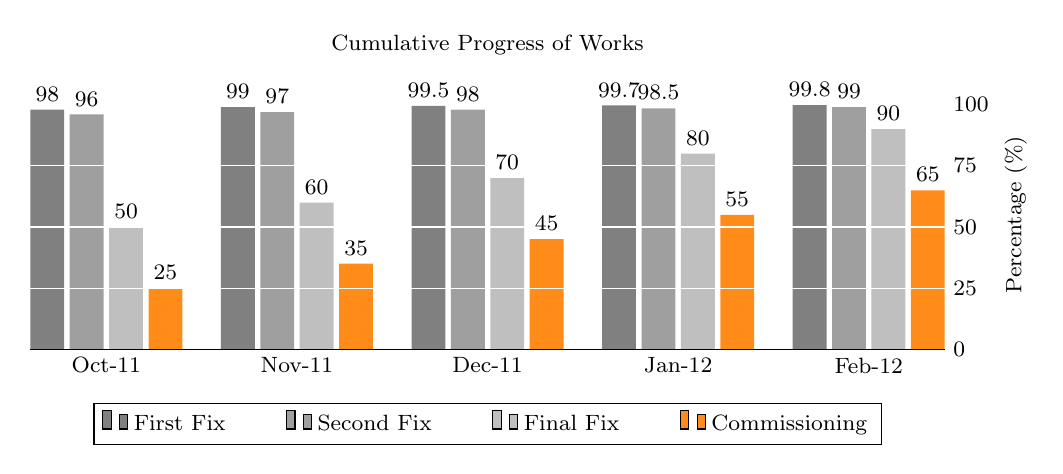
\begin{tikzpicture}
  \footnotesize
  \centering
  \begin{axis}[
        ybar, axis on top,
        title={Cumulative Progress of Works},
        height=5cm, width=13.2cm,
        bar width=0.43cm,
        ymajorgrids, tick align=inside,
        major grid style={draw=white},
        enlarge y limits={value=.1,upper},
        ymin=0, ymax=100,
        axis x line*=bottom,
        axis y line*=right,
        y axis line style={opacity=0},
        ytick={0,25,50,75,100},
        tickwidth=0pt,
        legend style={
            at={(0.5,-0.2)},
            anchor=north,
            legend columns=-1,
            % adds space between the legends
            /tikz/every even column/.append style={column sep=0.7cm}
        },
        ylabel={Percentage (\%)},
        symbolic x coords={
           Sep-11,Oct-11,Nov-11,Dec-11,
           Jan-12,Feb-12,
           Mar-12,
          Apr-12},
       xtick=data,
       nodes near coords={
        \pgfmathprintnumber[precision=2]{\pgfplotspointmeta}
       }
    ]
    \addplot [draw=none, fill=gray] coordinates {
      (Oct-11, 98)
      (Nov-11,99)
      (Dec-11,99.5)
      (Jan-12,99.7)
      (Feb-12,99.8)
       };
   \addplot [draw=none,fill=gray!75!white] coordinates {
      (Oct-11, 96)
      (Nov-11,97)
      (Dec-11,98)
      (Jan-12,98.5)
      (Feb-12,99)
        };
   \addplot [draw=none, fill=gray!50!white] coordinates {
      (Oct-11, 50)
      (Nov-11, 60)
      (Dec-11, 70)
      (Jan-12, 80)
      (Feb-12, 90)
            };
    \addplot [draw=none, fill=orange!90!white] coordinates {
      (Oct-11, 25)
      (Nov-11, 35)
      (Dec-11, 45)
      (Jan-12, 55)
      (Feb-12, 65)
          };
    \legend{First Fix,Second Fix,Final Fix,Commissioning}
  \end{axis}
  \end{tikzpicture}

\caption{\protect\raggedright Cumulative progress for all MEP works. Notice the slower rate of production during the last three months.}
\label{fig:tufte-overall}
\end{figure}

\section{Graph Design}
A good graph is uncluttered, clear and focused.

\subsection{Axis Lines}

Most problems with graphs arise from misuse of axes: too heavy, too long, wrong intersection,
ambiquous breaks or too confusing increments and incorrect proportions. An axis is a ruler that established
regular intervals for measuring the information provided. Axes may emphasize, diminish, distort, simplify
or clutter the information.

\clearpage
\begin{multicols}{2}
\subsection{Axis Length}

Graphs should utilize their space around them, as the graph itself is mostly white space. In publications the journal might want to minimize the cost of printing. An axis should not extend beyond the labeled unit od minor tick closest to the last data point.
\columnbreak
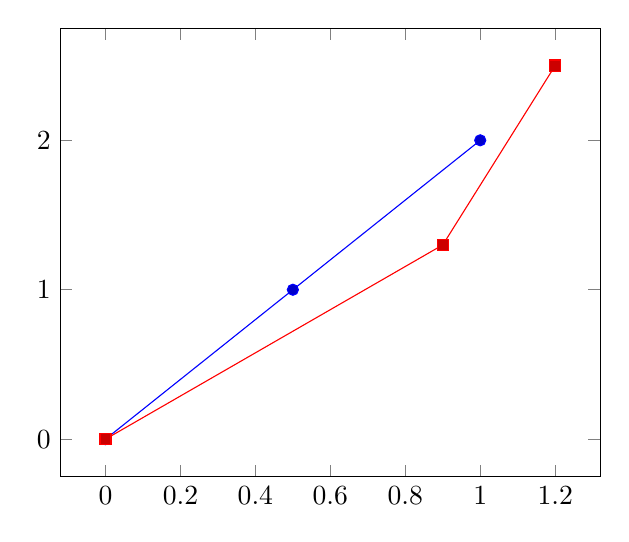
\begin{tikzpicture}
\begin{axis}
\addplot coordinates {
(0,0)
(0.5,1)
(1,2)
};
\addplot coordinates {
(0,0)
(0.9,1.3)
(1.2,2.5)
};
\end{axis}
\end{tikzpicture}
\end{multicols}














  \chapter{Wrapped Illustrations}
\label{ch:wrapped}
\parindent2em
\let\onepar\lorem

Wrapped figures are not in vogue and most users of \latex avoid them.
If you are planning to have a more traditional book design wrapped figures might be more appropriate. Traditional typographers used
all sorts of styles to achieve wrapped figures which conserved paper. 
The best way to achieve it is to use Donald Arseneau's |wrafig| package \citep{wrapfig}.

\begin{wrapfigure}{l}{3.2cm}
    \includegraphics[width=3cm]{./images/amato.jpg}
    \caption{\footnotesize Wrapped figures}
\end{wrapfigure}

Get prepared to do a lot of manual adjustments, see your figures disappear on page refreshes and reruns. It is also recommended that you do your final adjustments once you are happy with the contents of your document and these final adjustments will not start jumping around. 
After a while though you get the hang of it and by minor adjustments you can really achieve great results. The manual uses \verb+everypar+ to insert commands for the shaping of the paragraphs that \emph{follow} the wrapped figure.

The package provides the environments \pkg{wrapfigure} and \pkg{wraptable} for typesetting a
narrow float at the edge of the text, and making the text wrap around it. The |wrapfigure|
and |wraptable| environments interact properly with the \verb+\caption+ command to produce
proper numbering, but they are not regular floats like \textit{figure} and \textit{table}, so be aware to do manual adjustments. If you do not take care 
they may also be printed out of sequence with the regular floats.

The |wrapfigure| environment  provides one of those monster locomotive type commands that stresses one's memory as it provides for four parameters.
 
The four param
for \verb+\begin{wrapfigure}+, two optional and two required, plus the text of the figure, with a caption perhaps.

\begin{macro}{wrapfigure}
\end{macro}

|\begin{wrapfigure}[12]{r}[34pt]{5cm}\meta{figure}\end{wrapfigure}|

  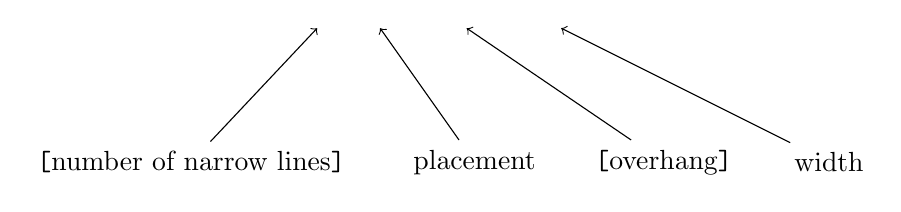
\begin{tikzpicture}[xshift=-15pt]
    \node (number) at (0mm, 0mm) {\oarg{number of narrow lines}};
    \node (placement) at (36mm, 0mm) {\marg{placement}};
    \node (overhang) at (60mm, 0mm) {\oarg{overhang}};
    \node (width) at (81mm, 0mm) {\marg{width}};
    \begin{scope}[->]
    \draw (number) -- (16mm, 17mm);
    \draw (placement) -- (24mm, 17mm);
    \draw (overhang) -- (35mm, 17mm);
    \draw (width) -- (47mm, 17mm);
    \end{scope}
  \end{tikzpicture}


First we will look at placing the figure without the use of optional commands.


\begin{verbatim}
\begin{wrapfigure}{r}{.4\textwidth}
    \includegraphics[width=.4\textwidth]{./path/file}
    \caption{\footnotesize Wrapped figures}
\end{wrapfigure}
\end{verbatim}

From the four parameters the first one indicates if the figure is to be typeset left or right.

\begin{verbatim}
\begin{wrapfigure}{l}{\imagewidth}
    \includegraphics[width=\imagewidth



]{./graphics/parasol-01}
    \caption{\footnotesize Wrapped figures}
\end{wrapfigure}
\end{verbatim}


\begin{wrapfigure}[18]{I}[0.1pt]{85pt}
    \captionsetup{name=Fig.}
    \vskip-10.5pt plus 2pt minus 2pt\relax
    \includegraphics[width=83pt]{./images/parasol-01.jpg}
    \caption{Wrapped figures, parameters set at \texttt\{l\}\{90pt\}.}
\end{wrapfigure}

Changing the parameters to suit we now have the illustration floating to the left. Allowing for the figure to be approximately two point  wider than the actual graphic, will leave a bit more margin. If the figure is end low in the page you need to be careful, that it does not disappear, as you will not get any warning.

The first parameter we are going to use an optional parameter is the one that determines the number of narrow lines. The format is \verb+[narrowlines]{l}{90pt}+. Think of this parameter as a fine tuning parameter and do not touch it until after your final draft is ready. If you see indented lines at the beginning of the page that follows the wrapped figure, reduce the number of lines, until you get satisfactory results.

The second optional parameter, comes after the \texttt{\{r\}[overhang]} parameter.

The second optional parameter (\#3) tells how much the figure should hang out into
the margin. The default overhang is given by the length \verb+\wrapoverhang+, which is 0pt
normally but can be changed using the command |\setlength|. For example, to have all wrapped figures you can 
use the space reserved for marginal notes,

\begin{verbatim}
\setlength{\wrapoverhang}{\marginparwidth}
\addtolength{\wrapoverhang}{\marginparsep}
\end{verbatim}

Again not recommended. The best approach is to specify the figures with \textbf{O} or \textbf{I}, let them float and if the results are
not very good then make manual adjustments. Get prepared to spend at least 5-10 minutes fiddling with the final result.

When you do specify the overhang explicitly for a particular figure, you can use a
special unit called \string\width meaning the width of the figure. For example, [0.5\string\width]
makes the center of the figure sit on the edge of the text, and [\string\width] puts the figure
entirely in the margin (and the adjacent text is indented by just \string\columnsep). This
\texttt{\string\width} is the actual width of the wrapfigure, which may be greater than the declared
width.

\begin{figure}[tb]
\includegraphics[width=\textwidth]{./graphics/chiefs.jpg}
\caption{Chiefs of Kelau or Kelaou.}
\label{fig:chiefs}
\end{figure}

\begin{figure}[p]
\centering

\includegraphics[width=0.8\textwidth,height=0.9\textheight, keepaspectratio]{./images/parasol-01.jpg}
\caption{Chiefs of Kelau or Kelaou.}
\label{fig:parasol-01}
\end{figure}

\section{Balancing the illustrations}

Illustrations come in various sizes, but in general they need to flow with the text. Place figures on top of the page and figures that would dominate the text on their own page. For example Figure~\ref{fig:chiefs} was allowed to float to the top of a page whereas Figure~\ref{fig:parasol-01} was placed on its own page, as I thought it will overwhelm the text if shown in a large size. However the same figure seems perfectly alright as a wrapped figure.

\begin{texexample}{}{}
\begin{wrapfigure}{I}{0pt}
    \includegraphics[width=75pt]{./images/parasol-01.jpg}
 \end{wrapfigure}
\lipsum[1-2]
\begin{wrapfigure}{l}{0pt}
    \includegraphics[width=75pt]{./images/parasol-01.jpg}
 \end{wrapfigure}
\lipsum[1-2]
\end{texexample}



\begin{texexample}{}{}
\begin{wrapfigure}{l}{0pt}
    \includegraphics[width=70pt]{./images/parasol-01.jpg}
    \includegraphics[width=70pt]{./images/parasol-01.jpg}
 \end{wrapfigure}

\lipsum[1-3]\lorem
\end{texexample}




\begin{texexample}{}{}
\begin{wrapfigure}[13]{L}{0pt}
    \includegraphics[width=100pt]{./graphics/conicalbasket.png}
\end{wrapfigure}

\onepar\onepar\onepar

\end{texexample}




  \chapter{Colors}

\newthought{The figure below, shows the wavelengths} in nm of the visible light. It has been drawn using the \docpkg{xcolor} package and the native \latex environment \cmd{picture}. The colors can be typest using the wavelength of light.

\smallskip

\begin{texexample}{}{}
  \hbox{\color{thered} A TesT}
\end{texexample}




\newcount\WL \unitlength.75pt

\begin{figure}
\hskip-3pt\scalebox{0.9}{
\noindent

\begin{picture}(460,60)(355,-10)
\sffamily \tiny \linethickness{1.25\unitlength} \WL=360
\multiput(360,0)(1,0){456}%
{{\color[wave]{\the\WL}\line(0,1){50}}\global\advance\WL1}
\linethickness{0.25\unitlength}\WL=360
\multiput(360,0)(20,0){23}%
{\picture(0,0)
\line(0,-1){5} \multiput(5,0)(5,0){3}{\line(0,-1){2.5}}
\put(0,-10){\makebox(0,0){\the\WL}}\global\advance\WL20
\endpicture}
\end{picture}}
\caption{The visible spectrum nm}
\end{figure}

The |xcolor| package provides numerous macros for typesetting colors, using a variety of methods and color schemes. For example we can use the command \cs{color} to print a text sample in color.
\newlength\pull

\def\colorSample#1{%
\leavevmode
\parindent0pt
   \def\colorRule{\color[wave]{#1}\rule{\textwidth}{0.4pt}} 
   \colorRule
%% set to the width of the box
   \settowidth\pull{\framebox{\Large #1 nm}}
%% pull by one em
   \addtolength\pull{1em}
   \hskip -\pull{\color[wave]{#1}{{\framebox{\Large #1 nm}}}}%
   %% add story
   \hskip1em\noindent\onepar\par
   \colorRule
}
\bgroup
\colorSample{385}
\colorSample{809}
\egroup


\section{Specifying colors by name}

The easier way to specify colors is to use the pre-build names available
with the package drivers.











  
  \chapter{A more flexible and robust method of defining functions with LaTeX3 and xparse}
\label{ch:xparse}

The \LaTeX3 Team developed the package \pkg{xparse} to provide document level 
authors with some powerful commands that extend those such as \cs{newcommand}
of \latexe. The code is been stable and the interface is not expected to change. 
Although targetted at document level, the commands offered can be used effectively to produce code used in packages.\footnote{\protect\url{http://tex.stackexchange.com/questions/98152/always-use-newdocumentcommand-instead-of-newcommand}} The functions offered by the package enable commands with star, or optional arguments to be produced easily. 

\begin{docCommand}{DeclareDocumentCommand}{\marg{function}\marg{argument specification}\marg{code}}
This family of commands are used to create a document-level \emph{function}. The argument
specification for the function is given by \textit{arg spec}, and expanding to be replaced by the
\textit{code}. Unlike \latex's definition commands, all xparse commands take two arguments.
The first one is the \textit{argument specifier}, and the second is the \textit{code.}
\end{docCommand}

\begin{texexample}{DeclareDocumentCommand}{l3:1}
\DeclareDocumentCommand \foo { m o m } { 
    arg 1 = #1, arg 2 = #2,  arg 3 = #3 }
\foo{A}[B]{C}  

\foo{A}{B}    
\end{texexample}

In the example above |{m o m}| is the argument specifier. It tells the function  to expect, two mandatory arguments and one optional denoted by the letter \textbf{o}. There are many more specifiers. For example \textbf{O} takes an parameter as a default value.\index{argument specifier}

\begin{texexample}{DeclareDocumentCommand}{l3:1}
\DeclareDocumentCommand \foo { m O{\ldots} m } { 
    arg 1 = #1, arg 2 = #2,  arg 3 = #3 }
\foo{A}[B]{C}  

\foo{A}{B}    
\end{texexample}

The argument markers can be entered in any order. In the following example we will also add an optional argument in a curly bracket. Although this is frowned upon in certain contexts it is useful. Consider the case of a chapter title that also has a subtitle. \docAuxCommand*{Chapter}, it maybe more natural and useful to have input of the form, as shown in Example~\ref{l3:g}. 

\begin{texexample}{DeclareDocumentCommand}{l3:g}
\DeclareDocumentCommand \MyChapter { o m g } { 
\centering #2\par #3\par }
    
\MyChapter{THIS IS THE MAIN TITLE}{This is a subtitle}  

\MyChapter[]{THIS IS THE MAIN TITLE}{This is a subtitle}        
\end{texexample}

\begin{texexample}{DeclareDocumentCommand}{l4:g}
\DeclareDocumentCommand \MyChapter {s o m g } { 
\IfBooleanTF {#1} {\gdef\fonta{\bfseries\selectfont}}{\gdef\fonta{}}
\IfNoValueTF {#2} {No option\par}{#2}

\centering {\fonta #3}\par #4\par 
  }   
\MyChapter{ THIS IS THE MAIN TITLE}  

\MyChapter*[short title]{THIS IS THE MAIN TITLE}{This is a subtitle}        
\end{texexample}

As you can see, it is fairly easy to produce starred and unstarred versions of commands as well as as any form of optional arguments. Let us now see some of the other command definition functions, before we continue with other specifiers.

\begin{docCommand}{NewDocumentCommand}{\marg{function}\marg{argument specification}\marg{code}}
will issue an error if \meta{function} has already been defined
\end{docCommand}

\begin{docCommand}{RenewDocumentCommand}{\marg{function}\marg{argument specification}\marg{code}}
For changing a definition,
issuing an error message if the macro does
not already exist.
\end{docCommand}


As the \cmd{\DeclareDocumentCommand} always updates a definition, it is used for the examples in this chapter to avoid any errors.

What sets the above commands apart from \latexe \cmd{\newcommand} is the argument specification.



\begin{texexample}{DeclareDocumentCommand}{l3:1}
\DeclareDocumentCommand \teststar {s o m } { 
\IfBooleanTF {#1}
  { \typesetnormalchapter {#2} {#3} }
  { \typesetstarchapter {#3} }
}  
\newcommand\typesetnormalchapter[2][]{
  normal chapter
}
\newcommand\typesetstarchapter[1]{
  #1
}
\teststar{Test}

\teststar*{test}
\end{texexample}    

    
The argument specification \textbf{m o m} in the example enables the function to accept three arguments, two mandatory and one optional. 


\section{Argument specifications}

The basic idea of an argument specification is that each argument is listed as a single letter. 
As the argument specification is a mandatory argument, a function with no arguments still needs an arg spec.

\begin{texexample}{Empty arg spec}{}
\DeclareDocumentCommand\atest{}{some text}
\atest
\end{texexample}

Manadatory arguments are created using the letter \textbf{m}.

\begin{marglist}
\item [m] Mandatory. This is a standard mandatory argument, which can either be a single token alone or multiple tokens surrounded by curly braces. Regardless of the input, the argument will
be passed to the internal code surrounded by a brace pair. This is the \pkgname{xparse} type
specifier for a normal \tex argument.
\end{marglist}

\begin{texexample}{Mandatory Values, verbatim}{}
\DeclareDocumentCommand\testverbatim{ v }{
    \ttfamily#1
}
\testverbatim+ \this is a test +

\testverbatim * &^%$#\test *

\testverbatim{\ttfamily \bfseries\normalfont test}
\end{texexample}

The \textbf{l} specifier reads its argument, until it encounters a left brace. It is equivalent to \tex \# argument. Can be used basically for |\hbox| type comands.

\begin{texexample}{Mandatory arguments l-specifier}{}
\DeclareDocumentCommand\myhbox{ l }{
   \hbox to \dimexpr(#1)\relax
}
\fbox{\myhbox 12pt+1em+13ex  {test}}
\end{texexample}



\begin{marglist}
\item [o] Optional argument in  []. Returns |-NoValue-| if not present.
\item [O] As for \textbf{o}, but returns \meta{default}, if no value is given. Should be given as |O{default}|.

\item [s] Starred version
\item [v] Verbatim. Reads an argument “verbatim”, between the following character and its next occurrence,
in a way similar to the argument of the LATEX2" command \cmd{\verb}. Thus
a v-type argument is read between two matching tokens, which cannot be any of
\%, \#, \{, \}, \^ or  . The verbatim argument can also be enclosed between braces,
\{ and \}. A command with a verbatim argument will not work when it appears
within an argument of another function.
\item [l] An argument which reads everything up to the first open group token: in standard
\latex this is a left brace.
\item [u] Reads an argument “until \meta{tokens} are encountered, where the desired \meta{tokens}
are given as an argument to the specifier: |u|\meta{tokens}.
\item [d] An optional argument that is delimited. 
\item [D] As for d, but returns \meta{default} if no value is given: D\meta{token1} \meta{token2}\marg{default}.
Internally, the o, d and O types are short-cuts to an appropriated-constructed D
type argument.
\item [t]  An optional \meta{token}, which will result in a value \cs{BooleanTrue} if \meta{token} is 
            present and \cs{BooleanFalse} otherwise. Given as \meta{token}.
\item [g] An optional argument given inside a pair of \tex group tokens (in standard \latex,
              \{ . . . \}, which returns |-NoValue-| if not present.
\item [G] As  for \textbf{g} but returns \meta{default} if no value is given: |G|\marg{default}.
\end{marglist}

\begin{texexample}{Default Values}{}
\DeclareDocumentCommand\testcolor{ O{red} m }{
    \textcolor{#1}{#2}
}
\testcolor{This is typeset in red}
\testcolor[blue]{This is typeset in blue.}
\end{texexample}

\section{Testing special values}

The optional arguments of a function defined using |xparse| use dedicated variables to return
information about the naure of the argument received.

\begin{docCommand}{IfNoValueTF}{\marg{argument}\marg{true code}\marg{false code}}
The function tests if the argument has a value and executes the true of false code, by means
of a |-NoValue-| marker. 
\begin{texexample}{special values}{}
\DeclareDocumentCommand\doccmd{O{red} m}
    {
        \IfNoValueTF{#1}
            {\doccmdnocolor{#1}}
            {\doccmdcolor{\textcolor{#1}{#2}}}
     }
\newcommand\doccmdnocolor[1]{#1}
\newcommand\doccmdcolor[2]{#1 #2}     
This is \doccmd[blue]{text}  and this is \doccmd{text}.   
\end{texexample}
\end{docCommand}

\begin{texexample}{special values}{}
\DeclareDocumentEnvironment{allbold}{o}
    {
        \bfseries 
        \IfNoValueTF{#1}
            {\color{red}}
            {\color{#1}}
    }
    {                 }
\begin{allbold}[magenta]
\lorem
\end{allbold}
\end{texexample}

\begin{texexample}{variants}{ex:variants}
\ExplSyntaxOn
\cs_set:Npn \foo_something:Nn #1#2 {
   \csname\expandafter#1\endcsname{blue}{a a a} 
   { #2}
  }
\cs_generate_variant:Nn \foo_something:Nn { c }
%\meaning\foo_something:cn
\ExplSyntaxOff
\lorem


\end{texexample}



  \cxset{chapter name = Chapter}

\chapter{The \texttt{picture} Environment}
\label{pictureenvironment}
\index{environments=picture}
\index{packages=picture}

When TeX was developed, the notion of graphic output was very limited, although Knuth presented a method
using boxes to draw primitive commands at any point on the page. This of course is achieved using zero width or height |\hbox| or |\vbox| commands. LaTeX uses a similar approach with the picture environment. 
The |picture| environment comes straight out of the box and can be used to draw simple figures. For more sophisticated graphics |TikZ| is a better choice. It can be used in package documentation and simple tasks. The learning curve for using it is minimal.

Using the picture environment is much easier to code for drawing shapes or rulers around sectioning commands.
This type of heading is very popular in many modern books. Figure~\ref{fig:picture-sections}

\begin{figure}[htbp]
\includegraphics[width=\textwidth]{./images/picture-sections.jpg}
\caption{A section with some fancy lines around the text. From \textit{Probabilities and Statistics for Engineers and Scientists}, by Walpole \textit{et.al}, 2011. }
\label{fig:picture-sections}
\end{figure}

Of course this is also achievable without the picture environment, simpy using TeX commands or with tikZ. From graphics point of view, the environment is also useful for short mathematical diagrams.

\section{The Basic Commands}

\begin{docEnvironment}{picture}{}{}
\end{docEnvironment}
The |picture| environment is created using one of two commands.

\emphasis{picture}
\begin{teXXX}
 \begin{picture}(x, y). . . \end{picture}
\end{teXXX}

\noindent or

\begin{teXX}
  \begin{picture}(x, y)(x0,y0). . . \end{picture}
\end{teXX}

\begin{docCommand}{unitlength}{\marg{dim}}
Most people prefer the first type which they combine, with a |setlength| command that sets the \cs{unitlength}.
\end{docCommand}

The optional argument gives the coordinates of the point at the lower-left corner of the picture (thereby determining the origin). For example, if \cs{unitlength} has been set to 1mm, the command

\begin{texexample}{}{}
  \setlength\unitlength{1mm}
  \begin{picture}(40,40)(0,0)
    \put(10,30){\vector(0,-1){30}}
    \put(10,30){\vector(1,0){30}}
    \put(25,30.5){$a$} 
  \end{picture}
\end{texexample}

produces a picture of width 100 millimeters and height 200 millimeters, whose lower-left corner is the point (10,20) and whose upper-right corner is therefore the point (110,220). When you first draw a picture, you will omit the optional argument, leaving the origin at the lower-left corner. If you then want to modify your picture by shifting everything, you just add the appropriate optional argument.

\section{Text and Formulae}

%\begin{macro}{\linethickness}
%\begin{macro}{\thicklines}
%\begin{macro}{\thinlines}
Text and formulas can be written into a picture
environment with the \cs{put} command in the usual way. The line thickness can be
set by using \cs{linethickness}\marg{dim}. The command \cs{thinlines} is half the thickness of the \cs{linethickness} dimension and \cs{thicklines} is the current line width. The \cs{linethickness} does not change width of slanted lines
or circles as it is drawn using a font and would render badly.
%\end{macro}
%\end{macro}
%\end{macro}

\emphasis{thicklines}
\begin{texexample}{Text and Formulae}{}
\setlength{\unitlength}{0.8cm}
\begin{picture}(6,5)
 \thicklines
 \put(1,0.5){\line(2,1){3}}
 \put(4,2){\line(-2,1){2}}
 \put(2,3){\line(-2,-5){1}}
 \put(0.7,0.3){$A$}
 \put(4.05,1.9){$B$}
 \put(1.7,2.95){$C$}
 \put(3.1,2.5){$a$}
 \put(1.3,1.7){$b$}
 \put(2.5,1.05){$c$}
 \put(0.3,4){$F=
 \sqrt{s(s-a)(s-b)(s-c)}$}
 \put(3.5,0.4){$\displaystyle
 s:=\frac{a+b+c}{2}$}
\end{picture}
\end{texexample}



\setlength{\unitlength}{5cm}
\begin{picture}(1,1)
\put(0,0){\line(0,1){1}}
\put(0,0){\line(1,0){1}}
\put(0,0){\color{blue}\line(1,1){1}}
\put(0,0){\color{orange}\line(1,2){0.5}}
\end{picture}


\section{multiput and linethickness}
The \cmd{\multiput} is used to place multiple objects onto the picture. It has the general format shown below:

\setlength{\unitlength}{2mm}
\begin{picture}(30,20)
  \color{green}
   \linethickness{0.075mm}
   \multiput(0,0)(1,0){25}%
   {\line(0,1){20}}
   \multiput(0,0)(0,1){21}%
   {\line(1,0){25}}
   \linethickness{0.15mm}
   \multiput(0,0)(5,0){6}%
   {\line(0,1){20}}
   \multiput(0,0)(0,5){5}%
   {\line(1,0){25}}
   \linethickness{0.3mm}
   \multiput(5,0)(10,0){2}%
    {\line(0,1){20}}
   \multiput(0,5)(0,10){2}%
   {\line(1,0){25}}
\end{picture}



\begin{docCommand}{multiput} {(x,y) (Dx, Dy) \marg{n} \marg{object} }
The command |\multiput| allows to repeat
a \cmd{\put} a number of times.
\end{docCommand}

\begin{figure}
\setlength{\unitlength}{0.8cm}
\begin{picture}(6,5)
 \thicklines
 \put(1,0.5){\line(2,1){3}}
 \put(4,2){\line(-2,1){2}}
 \put(2,3){\line(-2,-5){1}}
 \put(0.7,0.3){$A$}
 \put(4.05,1.9){$B$}
 \put(1.7,2.95){$C$}
 \put(3.1,2.5){$a$}
 \put(1.3,1.7){$b$}
 \put(2.5,1.05){$c$}
 \put(0.3,4){$F=
 \sqrt{s(s-a)(s-b)(s-c)}$}
 \put(3.5,0.4){$\displaystyle
 s:=\frac{a+b+c}{2}$}
\end{picture}
\caption{Figures can have captions, if you enclose in a figure environment}
\end{figure}

\begin{figure}
\scalebox{0.7}{
\setlength{\unitlength}{0.5mm}
\begin{picture}(120,168)
\newsavebox{\foldera}
\savebox{\foldera}
(40,32)[bl]{% definition
\multiput(0,0)(0,28){2}
{\line(1,0){40}}
\multiput(0,0)(40,0){2}
{\line(0,1){28}}
\put(1,28){\oval(2,2)[tl]}
\put(1,29){\line(1,0){5}}
\put(9,29){\oval(6,6)[tl]}
\put(9,32){\line(1,0){8}}
\put(17,29){\oval(6,6)[tr]}
\put(20,29){\line(1,0){19}}
\put(39,28){\oval(2,2)[tr]}
}
\newsavebox{\folderb}
\savebox{\folderb}
(40,32)[l]{% definition
\put(0,14){\line(1,0){8}}
\put(8,0){\usebox{\foldera}}
\put(0.2,1.4)
{$\beta=v/c=\tanh\chi$}
}
\put(34,26){\line(0,1){102}}
\put(14,128){\usebox{\foldera}}
\multiput(34,86)(0,-37){3}
{\usebox{\folderb}}
\end{picture}}
\caption{Pictures can be scaled using \protect\textbackslash scalebox.}
\end{figure}

\section{Some examples}
Any vertex-symmetric graph is regular, but edge-symmetric graphs
need not be regular. For example,
\begin{verbatim}
$$\unitlength=10pt
\def\putdisk(#1,#2){\put(#1,#2){\disk{.4}}}
$\vcenter{
\hbox{\beginpicture(2,1.5)(0,0)
\putdisk(0,0)
\putdisk(2,0)
\putdisk(1,.5)
\putdisk(1,1.5)
\put(0,0){\line(2,1){1}}
\put(2,0){\line(-2,1){1}}
\put(1,.5){\line(0,1){1}}
\endpicture}}
\quad&\hbox{is edge-symmetric, not vertex-symmetric;}\cr
\noalign{\smallskip}
\vcenter{
\hbox{\beginpicture(2,2)(0,0)
\putdisk(1,0)
\putdisk(1,2)
\putdisk(0,.5)
\putdisk(0,1.5)
\putdisk(2,.5)
\putdisk(2,1.5)
\put(0,.5){\line(2,1){2}}
\put(2,.5){\line(-2,1){2}}
\put(0,.5){\line(2,3){1}}
\put(2,.5){\line(-2,3){1}}
\put(0,.5){\line(1,0){2}}
\put(0,1.5){\line(1,0){2}}
\put(1,0){\line(-2,3){1}}
\put(1,0){\line(2,3){1}}
\put(1,0){\line(0,1){2}}
\endpicture}}
\quad&\hbox{is vertex-symmetric, not edge-symmetric.}\qquad
 (\vcenter{\hbox{\beginpicture(1,2)(0,0)
\putdisk(.5,0)\putdisk(.5,2)\put(.5,0){\line(0,1){2}}\endpicture}}
\hbox{ is a maximal clique})\cr}$$
\end{verbatim}



\section{picture package}

The \pkg{picture} package by Heiko Oberdiek redefines the default \pkg{picture} macros and adds code that detects
whether such an argument is given as number or as length. In the latter case, the
length is used directly without multiplying with \cs{unitlength}. Th following
example i from the documentation of the package.

 \setlength{\unitlength}{1pt}
 \begin{picture}(\widthof{Hello World}, 10mm)
   \put(0, 0){\makebox(0,0)[lb]{Hello World}}%
   \put(0, \heightof{Hello World} + \fboxsep){%
   \line(1, 0){\widthof{Hello World}}%
 }%
 \put(\widthof{Hello World}, 10mm){%
   \line(0, -1){10mm}%
 }%
 \put(0,0){\line(966,259){8}}
 \end{picture}

The package |calc| is used for calculations or etex. The picture package requires that the package |calc| is loaded before
the |picture| package and is loaded correctly by |phd|.

The package also supports the packages \pkg{pspicture} and \pkg{pict2e}, but they must be loaded before package picture.

\section{pict2e}

The package pict2e by Hubert G\"a\ss lein, Rolf Niepraschk and Joseph Tkadlec extends the existing LATEX picture environment, using the familiar
technique (cf. the graphics and color packages) of driver files. In the user-level part of
this documentation there is a fair number of examples of use, showing where things are
improved by comparison with the Standard LaTeX picture environment.

The package is loaded automatically by |phd|.







  \parindent1em

\chapter{Boxes and glue in TeX}

\setlength{\columnsep}{2em}
{\it Once you understand \tex\rq{}s concept of glue, you may well decide that
it was misnamed; real glue doesn't stretch or shrink in such ways, nor does it
contribute much space between boxes that it welds together. Another word like
\emph{spring} would be much closer to the essential idea, since springs have a natural
width, and since different springs compress and expand at different rates
under tension. But whenever the author has suggested changing \tex's terminology,
numerous people have said that they like the word \emph{glue} in spite of its
inappropriateness; so the original name has stuck. }
\smallskip

{\hfill  ---  Donald E. Knuth}

\medskip   


\parindent1em




\newthought{Traditional typesetting} was a task that depended on assembling the types and inserting them one by one on holding frames. In a way it was an assembly of boxes.
The \tex typesetting system uses a similar model of boxes to typeset content but in addition it also uses the concept of glue to stretch or shrink the text so that it will look better typographically. Boxes contain
typeset objects, such as text, mathematical displays, and pictures, and glue
is flexible space that can stretch and/or shrink by amounts that are under
user control.

\begin{figure}[h]
\hbox{\drawfontbox{Qwerty}\drawfontbox{fjord}}
\caption{Everything is boxes.}
\end{figure}

\begin{center}
\printfontparams
\end{center}

\section*{Boxes}

Boxes in \tex have  a rectangular shape but have
three associated measurements called \emph{height}, \emph{width}, and \emph{depth}.
Figure \ref{fig:boxes} shows a 
picture of a typical box, showing its so-called \emph{reference point} and \emph{baseline}

The reason that they have three dimensions is that a character of text has normally three dimensions as shown in figure \ref{fig:boxes}. As characters need to be lined on a baseline, the depth provides a datum point on which they can be aligned and the depth provides a measure of the portion of the character that is below the baseline.


Boxes and glue are the main tools of \tex. The box can hold text and other items. Glue is simply spacing. It can be horizontal or veritcal spacing, and it can be made as rigid or as flexible as desired.



\textbf{One important feature of \tex is that it has no knowledge of the shape of the characters it typesets, just the dimensions of each character box.}


When \tex is typesetting, it is normally in horizontal mode, such as while
it is working on this paragraph. Otherwise, \tex can be in vertical mode, or
in math mode, or three others described in Chapter 13 of The \texbook.
Two low-level TEX commands for boxes are \cmd{hbox}, for a horizontal box,
and \cmd{vbox} for a box in vertical mode. In the latter, \tex is normally still
collecting material for display from right to left: it is not building up a
column of text, as in classical Chinese writing.

In both kinds of boxes, the result is an unbreakable object that acts
much like a single character. \tex reads input as a string of characters,
then breaks that string up in words, each of which forms a box. 
\emph{Word boxes}\index{word boxes}
are then collected into lines, lines into paragraphs, and paragraphs into a
page galley. The space between the words can be normal \emph{interword space},
or \emph{sentence-ending} space, which is somewhat larger in English-language
typesetting, and the space is normally glue, rather than of fixed size.

\tex has a sophisticated mathematical algorithm for figuring out the
best way to stretch or shrink interbox glue to optimize the appearance of
lines and paragraphs. Every so often, \tex checks to see whether it has
enough material saved on the growing page galley to fill a complete output
page, and it asynchronously (and effectively, unpredictably) calls the
output routine whose job it is to figure out where the page break should
happen, ship out a completed page to the |DVI|  file, and replace the galley by
whatever is left over.

In traditional \tex you  can force a line break with the carriage-return command \docAuxCommand{cr},
and a page break with the command \docAuxCommand{eject}, but \tex is an expert system,
and normally handles line and page breaking on its own. \latex provides its own commands such as \cmd{\clearpage} and \cmd{\newpage} and so do all other \tex based formats and systems.

\latex does not modify any of \tex's algorithms but simply it is a set of implemenation
macros.

\section{Units of measurement in TEX}

\tex allows you to specify sizes of typographical objects in any of nine different
units:


\begin{table}[htbp]
\begin{center}
\begin{tabular}{llp{5cm}}
\toprule
bp &big point &1 inch is exactly 72 bp; the PostScript pagedescription language uses these units, but just calls them points\\
cc &cicero: &1 cc is exactly 12 didot points, and is thus the European  analogue of the pica\\
cm &centimeter: &1 in is exactly 2.54 cm\\
dd &didot point: &1 dd is (1238/1157) pt, and is a typographical unit common in some parts of Europe\\
in &inch: &an archaic unit, roughly the width of a man's thumb; it has been discarded by most countries, but still used in the USA and its sattelites.\\
mm &millimeter: &1 in is exactly 25.4 mm\\
pc &pica: &1 pc is exactly 12 pt\\
pt &printer's point: &1 in is exactly 72.27 pt\\ 
sp &scaled point: &1 pt is exactly $2^{16}$ = 65536 sp.\\
\bottomrule
\end{tabular}
\end{center}
\end{table}



The units can be separated from their numeric value with optional space, so
\texttt{3pc} and \verb*+3 pc+ are equivalent. The little half box in the latter is a convenient
way to indicate explicit spaces in typewriter text. It can be printed by typing \cmd{\char32} and a suitable font or using |\textvisiblespace|.

Internally, \tex\ stores dimensions as integral numbers of scaled points:
1 sp is tiny ---  smaller than the wavelength of visible light.\footnote{The visible light has wavelengths from 380--450 nm for violet up to 620--750 nm for red (sp = 280 nm} It is sometimes
useful to create objects that small so that they differ from empty objects,
but are nevertheless invisible. It also ensures that TeX will look the same irrespective on which computer you actually compiled your document.

\tex deals only with 32-bit integer words, and does not take advantage
of extra precision available on historical machines with larger words. The
lower 16 bits of a dimension can be viewed as a fractional number of points,
and the uppermost bit is needed for a sign (0 for plus, 1 for minus). That
leaves 15 bits to hold an integral number of points, but TEX only expects 14
to be used, so that addition of two dimensions does not overflow. Thus, the
largest dimension in TEX is exactly 214 + (1 26) points, or about 5.758  
meters or 18.89 feet. 

\tex has several kinds of special storage locations, called registers, numbered
from 0 to 255. For example,\cs{dimen0} can hold a fixed dimension,
which can be specified in any of the nine units of measurement that are
recognized by \tex.

Here is how you can assign a dimension to a register, and then have \tex
display it back for you:

\begin{dispListing}
\dimen1 = 25.4mm (*@\protect\footnote{You shouldn't assign dimenensions to primitive registers, but rather use one of the allocation schemes provided by \latex to do so.}  @*)
\the\dimen1
\end{dispListing}


Notice that \tex’s output is always in points, showing that it converts different
input units to a common system of measurement.

You can convert a dimension to the much-smaller units of scaled points
by assigning it to another kind of \tex register designed to hold signed integers,
the\cs{count0} through\cs{count255} registers:

\begin{texexample}{}{}
\bgroup
  \dimen4 = 1pt
  \count4 = \dimen4
  \the\count4
\egroup
\end{texexample}

{\noindent This time we get the size as \texttt{sp} as 65536 }


You might have noticed that the conversion from inches to points was not
quite what we claimed in the summary of \tex units. Here is how to see the
differences:

\verb+\dimen1 = 1in+


\section{Skip registers}
\index{registers!skip}
\begin{docCommand}{skip}{}
\tex glue is specified as a fixed dimension, and optionally, with a plus and/
or minus dimension. Along with \cs{dimen} registers, TEX has glue registers,
called \cs{skip0} through \cs{skip255}. Here is how you can save glue settings in
 registers, and ask \tex to display the contents of one of them:
\end{docCommand}

\begin{texexample}{Skip counters}{ex:skipcounters}
\bgroup
  \skip1 = 10pt
  \skip2 = 10pt plus 3pt
  \skip3 = 10pt minus 2pt
  \skip4 = 10dd plus 3dd minus 2dd
  \the\skip4
  % 10.70007pt plus 3.21002pt minus 2.14001pt.
\egroup  
\end{texexample}


The four sample glue settings store, respectively, \textit{fixed glue}, \textit{stretchable
glue}, \textit{shrinkable glue}, and \textit{flexible glue} that can both stretch and shrink,
but only up to a specified amount. Interword and intersentence spaces are
generally defined with glue like this, so that if more stretch or shrink of
\index{glue}\index{glue!flexibe}\index{glue!stretchable}\index{glue!shrinkable}

\begin{teX}
\dimen2 = 72.27pt
\count1 = \dimen1
\count2 = \dimen2
\showthe \count1
> 4736286.
\showthe \count2
> 4736287.
\end{teX}

The two values differ by the tiny value 1 \textit{sp}, so we can in practice ignore
that difference. If we use higher-precision arithmetic, we find the exact
decimal equivalents of the fractions as

\begin{teX}
4 736 286=65 536 = 72.269 989 013 671 875;
4 736 287=65 536 = 72.270 004 272 460 937 5;
4 736 286.72=65 536 = 72.27
\end{teX}


Actually \tex uses that last relation as the definition of the conversion of
inches to scaled points, so that our assignment of 1 in to \verb+\dimen1+ has to
be rounded to the nearest integral number of scaled points. That is why
in the round-trip conversion from decimal to binary and back to decimal,
1 in became 72.26999 pt. \tex guarantees that its output decimal numbers
are always converted on input back to the original binary numbers from
whence they came. For more on the story of \tex’s I/O conversions, see [3].


Both \tex and \latex define a number of predefined dimensions and these are discussed in the relevant Chapters discussing the \latex kernel. For example you may come across the \docAuxCommand{jot}, which is defined by \latex as:

\begin{teX}
\newdimen\jot
\jot=3pt
\end{teX}

\begin{texexample}{jot}{ex:jot}
\bgroup
\parindent\jot
This is some sample text with a one |\jot| left indentation. Which is really too small to see in a paragraph.
\egroup
\end{texexample}

Defining |\parindent=jot| we can see that the indentation almost disappeared. This is obvious since |\jot| is used normally for maths.

Glue is the binder that lets \tex\ do its job. This chapter discusses some
preset forms of glue and their uses. Along with glue parameters there are a
number of special commands for inserting glue. The most interesting have
different degrees of infinity, namely |\hfil|, |\hfill|, |\hfilneg|, |\hss|,
and their vertical counterparts. 

Because of the special spacing requirements of mathematics, \tex\ defines
skips and spacing that are valid in mathematics mode only. Examples are the
are the special preset |mu| glues of |\thickmuskip|,
|\medmuskip|, |\thinmuskip|.
The |\newskip| and |\newmuskip| commands allocate skip (or really glue)
or muskip registers respectively for special uses. For example the specific
glues surrounding section heads are held in glue registers. 

It should be noted that the various |\...muskip| do not cause horizontal
spacing in math mode by themselves. They are used with |\mskip| to actually
cause the insertion of the glue.

These are all various forms of horizontal (or math) mode commands that insert
infinite quantities of glue. |\hfil|, |\hfill|, |\hfilneg|, and |\hss| insert
|plus 1fil|, |plus 1fill|, |minus 1fil|, and |plus 1fil minus 1fil|. 
The first two are {\it stretch} glues, the third is {\it shrink} glue and the
last is both. It
should be noted that when \tex\ tries to stretch or shrink glue values, they
vary according to their value. If there exists both |fil| and finite value
glue in a box or line, then all the stretch if it is |plus| glue 
or shrink if it is |minus| glue will be in
the section with the |fil| glue. If there is |fill| glue and either |fil| or
finite glue, then all the stretch or shrink will be in the |fill| sections.
Similarly with |filll| glue, which is not supplied in as readily usable form.
The difference in behaviour between |\hfil| and |\hss| is that |\hss| glue
will allow the contents of a box to spill outside without resulting in an
overfull box while |\hfil| will only fill or push contents to the edge of the
box. The major use for these glues are to center or to force stuff to either
edge of a box.  For instance this

\begin{texexample}{}{}
\def\aline{\vrule \hfil one \hfil two \hfil three 
         \hfill four \hfil five \hfil six 
         \hfill seven \hfil eight \hfil nine\vrule}

\aline

This is a preset |mu| glue. |\medmuskip = 4mu plus 2mu minus 4mu| for use
with |\mskip|. This is \hbox{\strut\vrule$\mskip\medmuskip$\vrule}.
\end{texexample}

So far we have been using in our examples the primitive \tex |\skip| to allocate
skip registers. This is dangerous, as they might have been defined elsewhere and our
definitions will overwrite them. Plain \tex and \latexe provide an allocation scheme
where this is done automatically. 

\begin{docCommand}{newskip}{}
The command \cs{newskip}\meta{skip name} assigns a new skip or glue register to
the name |\<skip name>|. 

Glue values may be assigned to it by |\<skip name> [=] <glue>|.
This assigns a new muskip or muglue register to the name |\<muskip name>|. Glue
values may be assigned to it by |\<muskip name> [=] <muglue>|.

This is a preset |mu| glue. |\thickmuskip = 5mu plus 5mu| for use
with |\mskip|. This is \hbox{\strut\vrule$\mskip\thickmuskip$\vrule}.

This is a preset |mu| glue. |\thinmuskip = 3mu| for use
with |\mskip|. This is \hbox{\strut\vrule$\mskip\thinmuskip$\vrule}
\end{docCommand}


\newskip\hides 
\hides= -1000pt% plus 1fill

atest atest

\hskip\hides atest

\hides= -1000pt  plus 1fill

atest atest

\hskip\hides atest

|\vfil \vfill|

|\vfilneg|

|\vss|

These are the vertical analogues to the infinite horizontal glues and act in
much the same manner. See the section on |\hfil ...|.
 



\normalsize



\section{Glue}

\tex joins the boxes it creates with some special mortar as Knuth writes, called glue. To understand how glue works we will
borrow a figure from the \tex Book.

\begin{figure}
  \centering
  \includegraphics[width=0.9\linewidth]{./images/glue.png}
  \caption{Glue in \TeX}
  \label{fig:glue}
\end{figure}


\section{How to specify glue}

The usual way to specify \textit{glue} to \tex is
$<dimen>< plus~dimen><minus~dimen>$

where the plus and minus are optional and assumed to be zero if not
present; plus\index{glue!plus} introduces the amount of stretchability\index{glue!stretchability}, minus introduces the amount of shrinkability \index{glue!shrinkability}. 

For example, Appendix B of the TexBook defines \cs{medskip} to be an abbreviation for
|\vskip6pt plus2pt minus2p|. The normal-space component of glue must always be
given as an explicit dimen, even when it is zero. The ability of \TeX to stretch and shrink this glue has given it its beautiful looks. Strangely enough, although the algorithm is public it has not been used widely in other software.



\subsection{hfil and hfill}

{\obeylines
{This text will be flush left.\hfil}
{\hfil This text will be flush right.}
{\hfil This text will be centered.\hfil}
{Some text flush left\hfil and some flush right.}
{Alpha\hfil centered between Alpha and Omega\hfil Omega}
{Five\hfil words\hfil equally\hfil spaced\hfil out.}
}

Consider the following definitions:

\begin{verbatim}
\def\centerlinea#1{\hfil#1\hfill}
\def\centerlineb#1{\hfill#1\hfill}
\def\centerlinec#1{\hss#1\hss}
We define quickly a \cs{lineX}\footnote{Strange but my \LaTeX\ distribution has not got on. (This definition is from \texttt{plain.sty}}

\def\lineX{\hbox to\hsize}
\def\lineX{\hbox to\hsize}
\def\centerlinea#1{\hfil#1\hfil}
\def\centerlineb#1{\hfill#1\hfill}
\def\centerlinec#1{\hss#1\hss}

\lineX{\centerlinea{\test}}
\lineX{\centerlineb{\test}}
\lineX{\centerlinec{\test}}
\centerline{\test}
\begin{center}\test\end{center}

\end{verbatim}


\section{Specifying glue amounts}

\tex glue is specified as a fixed dimension, and optionally, with a plus and
or minus dimension. Along with \cs{dimen} registers, TEX has glue registers,
called \cs{skip0} through \cs{skip255}. Here is how you can save glue settings in
\tex registers, and ask \tex to display the contents of one of them:

\begin{teX}
\skip1 = 10pt
\skip2 = 10pt plus 3pt
\skip3 = 10pt minus 2pt
\skip4 = 10dd plus 3dd minus 2dd
\the \skip4
\end{teX}


\texttt{> 10.70007pt plus 3.21002pt minus 2.14001pt}

The four sample glue settings store, respectively, {\em fixed glue}, {\em  stretchable
glue}, {\em shrinkable glue}, and {\em flexible glue}  that can both stretch and shrink,
but only up to a specified amount. Interword and intersentence spaces are
generally defined with glue like this, so that if more stretch or shrink of  a
re underfull (too little text to fill the line), or overfull (too much text in the
line).



\section{Overfull lines}

Although overfull lines are reported in the \tex log file, they can be hard
to find in the typeset document if they only stick out a little. To make
them highly visible while you are fine tuning your final document, assign
the variable \cs{overfullrule} a nonzero dimension, such as 2 cm. \tex then
displays a solid black box, called a \emph{rule}, of that width in the right margin
on each line that is overfull. Using the \docpkg{microtype} package one can adjust the parameters to minimize this.

To make the rules disappear, simply remove it,
or comment out, the assignment, or reset its value to 0 pt. 

Just as you can assign dimension registers to count registers to convert
from points to scaled points, you can assign skip registers to dimension and
count registers to discard the flexible parts:


\begin{teX}
\skip1 = 10pt plus 3pt minus 2pt
\the\skip1
 \dimen1 = \skip1
\the \dimen1
\count1 = \skip1
\the \count1
\end{teX}




\section{More on glue in boxes}

Besides normal glue with fixed amounts of stretch and shrink, \tex also has
two kinds of glue that are \emph{infinitely} stretchable and shrinkable: \cs{hfil} and
\cs{hfill} in horizontal mode, and \cs{vfil} and \cs{vfill} in vertical mode. Notice that there two versions
of the commands, the one ends with one ell and the second one with two. The
two-ell forms are more flexible than the one-ell forms.

The boxes and glue model is powerful, and \tex's author, Donald Knuth,
has written that he views it as the key idea that he discovered when he
first sat down in 1977--1978 to design a computer program for typesetting.
For example, to set something flush left, put infinitely-stretchable glue on
its right. To set it flush right, put the glue on the left. For centered material,
put the glue on both sides. Here are four examples, with vertical
bars marking the ends of the horizontal box (boxes have no visible frames,
although it is possible to write \tex commands to give them such outlines,
and we use that feature shortly):





\section{Horizontal and vertical boxes}


\begin{docCommand}{hbox}{\marg{material}}
\end{docCommand}

Like their dimensions \TeX's boxes are not what one thinks when thinking of boxes. TeX's boxes come in basically two flavours, horizontal boxes and vertical boxes. An \cs{hbox} is created by the command \refCom{hbox}\marg{material}. It has the following properties:

\begin{enumerate}
\item The material is placed from left to right and it becomes a \textit{horizontal list}.\index{horizontal list}
\item The box \textbf{cannot be broken across lines}; it is an indivisible unit.
\end{enumerate}

An |hbox| can contain, characters, horizontal glue, horizontal leaders or other boxes. While in many cases these other boxes can be other |\hbox|es, |\vbox| can be used.


The \refCom{hbox} command has another form |\hbox to <dimen>|\marg{material}. This
creates a box whose width is the given (dimen). Thus |\hbox to lcm{<material>}|
will create a 1 inch wide box \hbox to 1cm{text}. However, we have to supply exactly 1 cm worth of
material to fill up the box; otherwise we end up with an error message. It is best
to consider this form of the command as a promise; we promise '\tex that we will
supply just enough material to fill up the box. 

We can place other hboxes in an hbox. By adding glue we can then move them left or right

\begin{texexample}{hbox and glue}{ex:hbox}
\bgroup
\Huge
\hbox to \textwidth{\hfill \hbox{\EOofficerI}\hbox{\EOofficerII}\hbox{\EOofficerIII} \hfill}

\hbox to \textwidth{\hfill \hbox{\EOofficerI}\hbox{\EOofficerII}\hbox{\EOofficerIII} \hfil}

\hbox to \textwidth{\hfill \hbox{\EOofficerI}\hfill \hbox{\EOofficerII}\hfill \hbox{\EOofficerIII} \hfill}
\egroup
\end{texexample}

The last command that affects the shape of an |\hbox| is 'spread(dimen)', which
spreads the box beyond its natural width. An |\hbox spread12pt|{(material)}
makes the box 12 points wider than its natural size. If the material in the box has
no flexibility, it cannot spread to fill up the additional space, resulting in an underfull
box. This is why 'spread' is normally used with flexible glues.

\begin{texexample}{hbox and glue}{ex:hbox}
\bgroup
\LARGE
\hbox to 5cm{\EOofficerI\EOofficerII\hfill\EOofficerIII}

\hbox spread5cm{\hfill\EOofficerI\hfill\EOofficerII\hfil\EOofficerIII}

\hbox spread9cm{\EOofficerI\hfill\EOofficerII\hfil\hfil\EOofficerIII}

\hbox spread7cm{\EOofficerI\hfill\EOofficerII\hfil\hfil\EOofficerIII} 


\makeatletter
\hb@xt@ 5cm {\EOofficerI\EOofficerII\hfill\EOofficerIII}
\makeatother
\egroup
\end{texexample}



Boxes can be moved up or down using |\raise| or |\lower|. Each of these primitives is followed by a dimension indicating how far the box can be lowered or raised.

Other material that can go in an hbox, is \textbf{vertical rules}. 

\subsection{The null macro}

The |\null| macro is defined both in Plain as well as LaTeX and generates an empty box. Its definition is:

\begin{teXXX}
\def\null{\hbox{}}
\end{teXXX}


\fbox{\hbox{This is a test}}

{
\fbox{\hsize=5cm
A test of a box at the end of a 2.0 inch line\par}

\fbox{\hsize=5.0cm in A test of a box at the end of a \hbox to 2cm{2.0 cm} line\par}

}

What happens when we have more than two boxes on a line? TeX will stuck them one under another. If they are enclosed within another hbox they will be inlined.



\begin{texexample}{}{}
\hbox to 1cm {A} \hbox to 1cm {B}

If we however, put them together in another |\hbox|, we get:

\hbox{\hbox to 1cm {A} \hbox to 1cm{B}}
\end{texexample}




An |\hbox| does not imply horizontal mode, so an attempt to start a paragraph with a box, for
instance
|\hbox to 0cm{\hss$\bullet$\hskip1em}Text ...|

will make the text following the box wind up one line below the box. It is necessary to switch
to horizontal mode explicitly, using for instance |\noindent| or |\leavevmode|. The latter is defined
using |\unhbox|, which is a horizontal command.


\begin{texexample}{}{}
\hbox to 0cm{\hss$\bullet$\hskip1em} Text ...


\leavevmode\hbox to 0cm{\hss$\bullet$\hskip1em} Text ...

\end{texexample}




\section{Kerning}


Using the command \cs{kern}, we can move boxes either left or right. Kerning is extensively used to build internal commands and we discuss it in more detail under the chapter for fonts.

\begin{docCommand}{kern}{\meta{dimen}}
A |\kern| is similar to glue [75], with two differences: (1) |\kern| is rigid; (2)
|\kern| specifies a point where a line, or a page, should not be broken. Since a box is
indivisible anyway, |\kern| is used in a box to indicate rigid spacing. It is interesting
to note that the same command, |\kern|, indicates horizontal spacing when used in
an |\hbox| and indicates vertical spacing when used in a |\vbox|.
\end{docCommand}
Consider two horizontal boxes, holding the letters A and V:
As you can observe, the letters AB are a bit afar, from what would be a visually pleasant arrangement, we can kern them as follows:
\medskip

\begin{teXXX}
\hbox{\Huge AV A\kern-5ptV}
\end{teXXX}
\medskip

Note that hbox, does not produce a frame. I~have used a frame |\fbox|, which will cover a bit later as well as scaled the image by 2, in order to see the effects more clearly.


\drawfontbox{\upshape\Huge FJord F\kern-5pt Jorp}





\noindent\begin{tabular}{ll}
|\hbox{\kern4pt A\kern8pt B\kern8pt C\kern4pt}| & \fbox{\hbox{\kern4pt A\kern8pt B\kern8pt C\kern4pt}} \\
~ &\\
\midrule
|\hbox{\kern4pt\raise1pt\hbox{A}|  & \fbox{\hbox{\kern4pt\raise1pt\hbox{A} \kern8pt BC\kern8pt\lower6pt\hbox{D} \kern4pt} \kern8pt BC\kern8pt\lower6pt\hbox{D}\kern4pt} \\
|\kern8pt BC|                      &\\
|\kern8pt\lower6pt\hbox{D}|        &\\
|\kern4pt}|                        &\\ 
|\kern8pt BC|                      &\\ 
|\kern8pt\lower6pt\hbox{D}|        &\\
|\kern4pt}| &\\
\midrule
\end{tabular}


\vbox{
\noindent\rule{\linewidth}{0.4pt}
\begin{minipage}{4.5cm}
 \begin{teXX}
\fbox{\hbox{\kern4pt A\kern8pt 
      B\kern8pt C\kern4pt}}
\end{teXX}
\end{minipage}
\hfill\hfill
\begin{minipage}{3cm}
\hfill\hfill\fbox{\hbox{\kern4pt A\kern8pt 
      B\kern8pt C\kern4pt}}
\end{minipage}

\medskip
\noindent\rule{\linewidth}{0.4pt}
}

Notice that an |\hbox| is constructed by setting its components side by side so that their \textit{baselines} are aligned. When \cs{raise}, \cs{lower} are used the baselines are no longer aligned. In such a case the baseline of the box is defined as the baseline shared by the components before any vertical movements. In the example above the box now has a depth, as a result of lowering |D|.


\vbox{
\noindent\rule{\linewidth}{0.4pt}
\begin{minipage}{4.5cm}
\begin{teXXX}
\hbox{\kern4pt\raise1pt\hbox{A} 
  \kern8pt BC\kern8pt
  \lower6pt\hbox{D} 
  \kern4pt} 
\end{teXXX}
\end{minipage}
\hfill
\begin{minipage}{3cm}
\fbox{\hbox{\kern4pt\raise1pt\hbox{A} 
\kern8pt BC\kern8pt\lower6pt\hbox{D} \kern4pt}}
\end{minipage}

\medskip
\noindent\rule{\linewidth}{0.4pt}
}



\noindent\textbf{Vertical boxes.}\quad A vertical box is build in a similar manner to that of a horizontal list, except it is composed of material in the \textit{vertical list}.
When horizontal boxes are added in the list, they are stuck on top of each other as shown in the example below. 
\medskip

\bgroup
\parindent0pt
\fbox{\vbox{\hsize=3cm\fbox{\hbox{ABCDEFGH}} \fbox{\hbox{AB}}}}
\egroup


\begin{docCommand}{vbox}{ to \meta{dimen}\marg{\meta{material}}}
Typesets a box in vertical mode.
\end{docCommand}

It is important to remember the two main differences between hboxes and vboxes. An hbox will expand to hold its material. If it need be it will overfill the line and produce an overful warning. A vbox will expand to hold its material. It is perfectly normal for a vbox to hold paragraphs, as shown. This is not possible with an hbox. However, the common pattern is for an |\hbox| to contain a |vbox| .

\begin{texexample}{hbox/vbox example}{ex:vbox}
\noindent\fbox{\vbox{\lorem\par\lorem\par}}

\hbox to \linewidth{\vbox{\lorem\par\lorem\par}}
\end{texexample}


\begin{docCommand}{hsize}{\meta{dimen}}
 Controls the width of text in a |vbox|.
\end{docCommand}

\noindent\textbf{Controlling the size of a vbox.}\quad What controls the size, is the containing environment. This in TeX, is specified using |\hsize|. In LaTeX this is controlled by an enclosing environment, maybe a minipage (which is build this way) or one of the page width parameters.


\begingroup
\parindent0pt
\fboxsep5pt
\hsize=3.9cm\footnotesize
\hfil\fbox{\vbox{\RaggedRight\lorem\par}} 
\hfil\fbox{\vbox{\RaggedRight\lorem\par}}
\hfil\fbox{\vbox{\RaggedRight\lorem\par}}\hfill
\endgroup
\captionof{figure}{Output to demonstrate the use of vboxes.}



The code to typest the boxes shown above follows:
\medskip
\emphasis{hsize}
\begin{teXXX}
\bgroup
\parindent0pt
\hsize=3.3cm\footnotesize
\hfil\fbox{\vbox{\lorem\par}} 
\hfil\fbox{\vbox{\lorem\par}}
\hfil\fbox{\vbox{\lorem\par}}
\hfill
\egroup
\end{teXXX}


Note, the use of \docAuxCommand{hsize}. We define the font size as |\footnotesize|. We have done this in order not to have overfull boxes--Latin words don't have a full set of hyphenation patterns in \latex. The macro |\lorem|, we have defined internally for this document. We place the code in a group in order not to affect the rest of the document.



\clearpage

\noindent\textbf{Vertical centering}\quad can be achieved by applying vertical infinite glue \cs{vfill}. In the example that follows, first we place two letters in individual |\hboxes| and we enclose them in a vbox. We apply |\vfill| both on top and at bottom.

\emphasis{\vfill}

\vbox{
\noindent\rule{\linewidth}{0.4pt}
\begin{minipage}{5cm}
\begin{teX}
\fbox{\vbox to 0.9cm{\vfil\hbox{M}\nointerlineskip\hbox{i}\vfil}} 
\end{teX}
\end{minipage}
\hfill
\begin{minipage}{3cm}
\hfill\fbox{\vbox to 0.9cm{\vfil\hbox{M}\nointerlineskip\hbox{i}\vfil}}\hfill\hfill 
\end{minipage}

\medskip
\noindent\rule{\linewidth}{0.4pt}
}



A |\vbox| can be combined with text and may appear anywhere within a paragraph. The baseline of the box will be aligned with the baseline of the current line.


\vbox{%
\noindent\rule{\linewidth}{0.4pt}}

\begin{teX}
A vbox can be placed within a paragraph \fbox{\vbox to 0.6cm{\vfil\hbox{M}\nointerlineskip\hbox{i}\vfil}} as shown here.


\hfill

A vbox can be placed within a paragraph \fbox{\vbox to 0.6cm{\vfil\hbox{M}
  \nointerlineskip\hbox{i}\vfil}} as shown here.

\end{teX}

\medskip
\noindent\rule{\linewidth}{0.4pt}






\noindent\textbf{Top alignment.}\quad\cs{vtop} is similar to a |\vbox|. The depth of this box is zero, since both A and B are capital letters. The width of this box is |\hsize|, since it contains text. 


\begin{codeexample}[]
\vtop{\hbox{A} \hbox{B}}
\end{codeexample}






Centering a picture in a box, both vertically and horizontally can be achieved using the methods we described so far.


\emphasis{hfill,hbox}
\begin{texexample}{}{}
     \fbox{%
          \vtop{\medskip
                    \hfill
                      \hbox{\includegraphics[width=1.5cm]{./images/amato.jpg}}%
                    \hfill 
                   \medskip%
                }%
      }%
\end{texexample}

\begin{texexample}{}{}
    \fbox{%
          \vtop{\medskip
                    \hfill
                      \hbox{\includegraphics[width=1.5cm]{./images/amato.jpg}}%
                      \hbox{\includegraphics[width=1.5cm]{./images/amato.jpg}}%
                      \hbox{\includegraphics[width=1.5cm]{./images/amato.jpg}}%    
                    \hfill 
                   \medskip%
                }%
      }%
\end{texexample}

Study the example a bit more carefully, as we have said earlier on that \cs{hbox}'es are stacked vertically, the reason why in the above example they are next to each other is that they are in an
\cs{fbox} which in turn is an \cs{hbox}  that can draw  frame around the box and is defined in the
\latex2e kernel.

So if we had only three images in hboxes we will get:

\begin{texexample}{Three Images Lined}{}
%\leavevmode
%\parindent30pt
\hbox{\includegraphics[width=1.5cm]{./images/amato.jpg}}%
\hbox{\includegraphics[width=1.5cm]{./images/amato.jpg}}%
\hbox{\includegraphics[width=1.5cm]{./images/amato.jpg}}%
\end{texexample}

An hbox does not start a paragraph. If we started a paragraph the behaviour will be different.

\begin{texexample}{Three Images Lined}{}
.\hbox{\includegraphics[width=1.5cm]{./images/amato.jpg}}%
\hbox{\includegraphics[width=1.5cm]{./images/amato.jpg}}%
\hbox{\includegraphics[width=1.5cm]{./images/amato.jpg}}%
\end{texexample}

If you notice carefully, we have started the paragraph by inserting a `.' before the first |\hbox|, an alternative way is to 
use |\leavevmode|. The effect of this command is to leave vertical mode, and to enter horizontal mode. Thus, if the mode is vmode (typically, outside any paragraph), a new paragraph is started. This paragraph may be flushed left, flushed right. 

\begin{texexample}{Three Images Lined}{}
\leavevmode
\hbox{\includegraphics[width=1.5cm]{./images/amato.jpg}}%
\hbox{\includegraphics[width=1.5cm]{./images/amato.jpg}}%
\hbox{\includegraphics[width=1.5cm]{./images/amato.jpg}}%

\meaning\leavevmode
\end{texexample}

The macro |\leavevmode| as its name implies forces \tex to leave vertical mode and enter horizontal mode. In this case the photos are just treated by \tex similarly to any character and tehy are typeset next to each other. 

\begin{docCommand}{kern}{}
If we wanted to add a bit of space between the horizontal images, we could use \cs{kern}
Kern again. This is from the book TeX for The Impatient page 157. You can use kern in math mode, but you cannot use the \texttt{mu} units. If you want to use \texttt{mu} units use \cs{mkern} instead.
\end{docCommand}

\emphasize{kern}
\begin{texexample}{}{}
\leavevmode
\hbox{\includegraphics[width=1.5cm]{./images/amato.jpg}}\kern10pt
\hbox{\includegraphics[width=1.5cm]{./images/amato.jpg}}\kern10pt
\hbox{\includegraphics[width=1.5cm]{./images/amato.jpg}}%
\end{texexample}

One needs to be careful as to where you issue |\leavevmode|. If it is in the middle of a paragraph it will have no effect.
\emphasize{This,is,some,text}
\begin{texexample}{Example with leavevmode}{}
This is some text
\leavevmode
\hbox{\includegraphics[width=1.5cm]{botticelli-34.jpg}}\kern10pt
\hbox{\includegraphics[width=1.5cm]{botticelli-34.jpg}}\kern10pt
\hbox{\includegraphics[width=1.5cm]{images/botticelli-34.jpg}}%
\end{texexample}

A very common way in \latex2e is to issue a |\par| command before |\leavevmode| to avoid this problem. Another way is to use
one of the |\ifvmode| or |\ifhmode| and act accordingly. We now fix our example and get what we want. 

\emphasize{par}
\begin{texexample}{}{}
This is some text
\par\leavevmode
\hbox{\includegraphics[width=1.5cm]{botticelli-34.jpg}}\kern10pt
\hbox{\includegraphics[width=1.5cm]{botticelli-34.jpg}}\kern10pt
\hbox{\includegraphics[width=1.5cm]{images/botticelli-34.jpg}}%
\end{texexample}

\begin{texexample}{}{}
   \HHUGE
   \fboxsep=0pt
   \fbox{%
          \vtop{\medskip
                    \hfill
                       \hbox{ H\kern10pt i\kern10pt j}%    
                       \hbox{ A\kern10pt C\kern10pt j}%
                    \hfill 
                   \medskip%
                }%
   }%
\end{texexample}

This example shows how letters are typeset and you can see that they are aligned at the baseline. They are no different than the eimage example that we have shown earlier, except we don't need the boxes.

\medskip

\vbox{
\noindent\rule{\linewidth}{0.4pt}
\begin{minipage}{4.9cm}
\begin{teX}
\centerline{$\Downarrow$}\kern 3pt%
\centerline{$\Longrightarrow$\kern 6pt% horizontal kern
  \textit{A note about kern}\kern 6pt
    $\Longleftarrow$}
\kern 3pt
\centerline{$\Uparrow$}  
\end{teX}
\end{minipage}
\hspace{0.3cm}
\begin{minipage}{4.5cm}
\centerline{$\Downarrow$}\kern 3pt%
\centerline{$\Longrightarrow$\kern 6pt% horizontal kern
  \textit{A note about kern}\kern 6pt
    $\Longleftarrow$}
\kern 3pt
\centerline{$\Uparrow$}
\end{minipage}

\medskip
\noindent\rule{\linewidth}{0.4pt}
}
\medskip

To make a point again, |\vbox| lines boxes at their bottom while, |\vtop| lines them at their top.

\medskip

\vbox{
\noindent\rule{\linewidth}{0.4pt}
\begin{minipage}{4.9cm}
\begin{teX}
 \hbox{\hsize=2cm \raggedright
\vbox to 0.5in{\hrule This box is .5in deep. \vfil\hrule}
\qquad
\vbox to 0.75in{\hrule This box is .75in deep. \vfil\hrule}
\qquad
\end{teX}
\end{minipage}
\hspace{0.3cm}
\begin{minipage}{4.5cm}
\hbox{\hsize=2cm \raggedright
\vbox to 0.5in{\hrule This box is .5in deep. \vfil\hrule}
\qquad
\vbox to 0.75in{\hrule This box is .75in deep. \vfil\hrule}
\qquad}
\end{minipage}

\medskip
\noindent\rule{\linewidth}{0.4pt}
}

\medskip


Trying the same with vtop

\medskip

\vbox{
\noindent\rule{\linewidth}{0.4pt}
\begin{minipage}{4.9cm}
\begin{teX}
 \hbox{\hsize=2cm \raggedright
\vbox to 0.5in{\hrule This box is .5in deep. \vfil\hrule}
\qquad
\vbox to 0.75in{\hrule This box is .75in deep. \vfil\hrule}
\qquad
\end{teX}
\end{minipage}
\hspace{0.3cm}
\begin{minipage}{4.5cm}
\hbox{\hsize=2cm \raggedright
\vtop to 0.5in{\hrule \smallskip This box is .5in deep. \vfil\hrule}
\qquad
\vtop to 0.75in{\hrule \smallskip This box is .75in deep. \vfil\hrule}
\qquad}

\hbox{\hsize=2cm \raggedright
\vbox to 0.5in{\hrule \smallskip This box is .5in deep. \vfil\hrule}
\qquad
\vbox to 0.75in{\hrule \smallskip This box is .75in deep. \vfil\hrule}
\qquad}
\end{minipage}

\medskip
\noindent\rule{\linewidth}{0.4pt}
}

\medskip

There are some other special macros defined by Plain TeX that we will only touch briefly here. One of them is \cs{underbar}{\index{Plain!\textbackslash underbar}.
The macro puts its argument into an hbox and underlines it.

\medskip

\vbox{
\noindent\rule{\linewidth}{0.4pt}
\begin{minipage}{4.9cm}
\begin{teX}
 \underbar{1,000,788.22}
\end{teX}
\end{minipage}
\hspace{0.4cm}
\begin{minipage}{4.0cm}
\medskip
\hfill\hfill{}\hspace*{1em}a1,000,700.22 \hfill

\smallskip

\hfill\[\underbar 1,000,788.22 \]\hfill
\end{minipage}

\medskip
\noindent\rule{\linewidth}{0.4pt}
}

\medskip


The \cs{everyvbox} command inserts a series of tokens at the beginning of every |\vbox|.


\medskip

\vbox{
\noindent\rule{\linewidth}{0.4pt}
\begin{minipage}{4.9cm}
\begin{teX}
 \everyvbox{$\bullet$}...
\end{teX}
\end{minipage}
\hspace{0.4cm}
\begin{minipage}{4.0cm}
\begingroup% Without this group, there are tons of problems!
   \everyvbox{$\bullet$}
   \global\setbox1=\vbox{This is a paragraph without an initial indent. It is   \the\hsize\ long lines.}
   \global\setbox2=\vtop{\copy1}
\endgroup
 \hbox{\box1} 

 \hbox{\box2}
\end{minipage}

\medskip
\noindent\rule{\linewidth}{0.4pt}
}

\medskip
Knuth in the TexBook Chapter 24, has some short description of the every commands. The `everyhbox` inserts a token list just before as its name implies a horizontal box.

Here is a short example. We define a `oneLineBox`, which is simply an hbox with some text and we add spread to spread the line. Using |\everybox| we add the letter \textbf{a} in each horizontal box. 


\tex considers the box overfull if the excess width of the box is larger than \cs{hfuzz} or \cs{hbadness} is less than 100. If I change  the badness to hbadness, I get 1000.

\medskip

\vbox{
\noindent\rule{\linewidth}{0.4pt}
\begin{minipage}{10.0cm}
\begin{teX}
 \begingroup
     \everyhbox{a}
     \def\oneLineBox#1#2%
     {%
          \hfuzz=0pt
          \overfullrule=0.25pt
          \setbox0=\hbox spread#2{#1}%
          \setbox1=\hbox{\the\badness}% 
          \setbox2=\hbox to 4.5cm{\box0\hfil\box1}%
          \box2
     }
     \oneLineBox{Badness of line }{-1em}
     \oneLineBox{Badness of line }{-0.54em}
     \oneLineBox{Badness of line }{-0.4em}
     \oneLineBox{Badness of line }{0em}
     \oneLineBox{Badness of line }{1em}
     \oneLineBox{Badness of line }{2em}
     \oneLineBox{Badness of line }{3em}
 \endgroup
\end{teX}
\end{minipage}


\begin{minipage}{10.0cm}
\begingroup
     \everyhbox{a}
     \def\oneLineBox#1#2%
     {%
          \hfuzz=0pt
          \overfullrule=0.25pt
          \setbox0=\hbox spread#2{#1}%
          \setbox1=\hbox{\the\badness}% 
          \setbox2=\hbox to 4.5cm{\box0\hfil\box1}%
          \box2
     }
     \oneLineBox{Badness of line }{-1em}
     \oneLineBox{Badness of line }{-0.54em}
     \oneLineBox{Badness of line }{-0.4em}
     \oneLineBox{Badness of line }{0em}
     \oneLineBox{Badness of line }{1em}
     \oneLineBox{Badness of line }{2em}
     \oneLineBox{Badness of line }{3em}
 \endgroup
\end{minipage}

\medskip
\noindent\rule{\linewidth}{0.4pt}
}

\medskip










\parindent1em




\section{More features of horizontal boxes}

Characters in the Latin alphabet have different shapes, and in most typefaces,
different widths. The letters \texttt{d f h k l t} have ascenders, making them
higher than the vowels \texttt{a e o u}, while the letters \texttt{f g j p q y} have descenders,
giving them added depth below the vowels. Similarly, an \texttt{m} is wider than
an \texttt{i}. 

\drawfontbox{(fjord)}

When \tex makes a normal horizontal box, the box width is the sum
of the widths of the characters, and the fixed parts of any glue, contained
in it. Shrink and stretch components of glue are discarded for the width
calculation. The box also has both a height above the baseline, the invisible
line on which the characters rest, and a depth below the baseline. The
depth is zero if there are no objects with descenders. The height and depth
are chosen from the largest vertical extents of the contained objects.

If you look carefully at typeset material, you will observe that, in most
typefaces, parentheses, brackets, and braces have both descenders and ascenders,
and the typeface designer usually makes their extents the maximum
among all of the characters in the design. This sample text shows
document: ( h g ) [ k j ] { l p }.

You can force TEX to choose a larger height and depth than normal when
you write a command for a horizontal box by ensuring that it has suitable
contents, such as an invisible vertical rule of zero width. The command

\verb+\hbox to 50pt {\vrule height 20pt depth 10pt width 0pt \it stuff}+

produces a box whose (invisible) outline looks like this: 

\hbox to 50pt {\vrule height 20pt depth 10pt width 0pt \it Great}

\drawfontbox{\kern 5pt\vrule height20pt depth 10pt width 1pt fjord}

The
three extents of the vertical rule can appear in any order, and any convenient
units.

In order to see the otherwise-invisible box edges in that example, we
used the \latex  built-in command \cs{fbox} to create a frame, and we eliminated
the default margin inside the frame by setting \cs{fboxsep = 0pt}. Plain \tex
does not have the \cs{fbox} command, but The TEXbook shows how to make
something like it on pp. 223 and 321.

One particular zero-width vertical rule is convenient for ensuring that
separate boxes all get the same height and depth. It has the height and
depth of parentheses in the normal prose font, and is given the macro name \refCom{strut}.
Its definition in the plain.tex file of macro definitions is roughly
equivalent to this:

\begin{docCommand}{strut}{}
\end{docCommand}

\begin{teX}
  \def \strut {\vrule height 8.5pt depth 3.5pt width 0pt}
\end{teX}

We insert a |\vrule| at the figure on the left below with a height of 20pt and a depth of 10pt. You can observe the difference on the right box, without the |\vrule|. The \textit{strut} is the blue line, which we gave a width of one point to make it visible. Real life struts, would have a width of 0pt and will not be visible. 

\drawfontbox{\kern5pt{\color{blue}\vrule height20pt depth 10pt width 1pt} fjord}
\drawfontbox{fjord}



\section{Horizontal alignment of boxes in TEX}
\fboxsep0.4pt

When horizontal boxes are set together, they are treated as separate words,
and therefore spaced accordingly. The input
\verb+ \fbox{one} \fbox{two} \fbox{three} \fbox{four}  +
produces  \fbox{one} \fbox{two} \fbox{three} \fbox{four}. As the example shows, we can put spaces
between them, or run them together so that they fit tightly.


\section{Vertical boxes in TEX}


\begin{minipage}{2.0in}
\begin{verbatim}
\noindent
\fbox{%
  \it
  \hbox to 80pt{%
     \parindent = 0pt
     \vbox to 30pt {%
         left text
         \vfil
         more left text%
     }%
  }%
}%
\end{verbatim}
\end{minipage}


%\noindent
\fbox{%
  \it
  \hbox to 80pt{%
     \parindent = 0pt
     \vbox to 30pt {%
         left text
         \vfil
         more left text%
     }%
  }%
}%

Firstly we use a noindent to ensure that the box is not indented. If you comment the\cs{fbox} out, you can see that the right amount of space has been left in the paragraph above.

\mbox{}
 
\noindent
\fbox{%
\it
\hbox to 80pt{%
\parindent = 0pt
\hsize = 80pt
\vbox to 30pt {\hfill right text
\vfil
\hfill more right text}
}%
}%



\noindent
\fbox{%
\it
\hbox to 80pt{%
\parindent = 0pt
\hsize = 80pt
\vbox to 30pt {\hfil center text
\vfil
 more center text \hfil}
}%
}%

We can aslo center the text for both lines, by modifying the code slightly.
\begin{teX}
\noindent
\fbox{%
\it \hbox to 80pt{
   \parindent = 0pt
   \hsize = 80pt
   \vbox to 30pt {
   center text \hfill
    \vfil
    \hfil more center text}
   }%
}%
\end{teX}


\noindent
\fbox{%
\it
\hbox to 80pt{%
\parindent = 0pt
\hsize = 80pt
\vbox to 30pt {\hfil center text
\vfil
\hfil more center text}
}%
}%



\chapter{Boxes with \protect\LaTeXe}

The \tex primitive commands have been abstracted by \latexe into more user friendly commands that are easier to use. One other reason for using these \LaTeX\ commands is that they are ``color safe''. Later on we will see other possibilities given by the \pkgname{color} or \pkgname{xcolor} package for drawing colored boxes, but we want to recall that the code for |\makebox| and the like has already a protection mechanism for colors, which the primitive commands do not have. \latexe also provides boxes that are self-aware of the width of their contents. For example |\fbox| will frame its contents in an |\hbox|. This simple task is very convoluted to achieve using basic \tex commands. 

\begin{docCommand}{framebox} {\marg{dim}}
One useful box command provided by \latex2e is \cmd{\framebox}. This command builds a box with any material you want to provide it with. The contents of this box are unbreakable, and as far as \tex is concerned it is treated the same way as it would treat a letter. 
\end{docCommand}

\begin{docCommand}{fboxsep}{\marg{dim}}
\end{docCommand}
\begin{docCommand}{fboxrule}{\marg{dim}}
Two associated lengths control the width of the rule and the space around the contents. We can change their default value by using |\setlength{\fboxsep}{0pt}| or just simply |\fboxsep=0pt| or even |\fboxsep0pt|. 
\end{docCommand}


Another interesting property is this: \emph{the contents of a box need not lie inside it}. You may have
noticed that, given the contents as an argument, the
|\framebox| command sets the dimensions of the box
to those of the contents (in reality, to the ``sub-boxes"
that compose the contents). But you can define the
dimensions explicitly as well. For example,

\begin{texexample}{framebox example}{ex:framebox}
|\framebox[13em]{Some text}|

\framebox[13em]{Some text}

\fcolorbox{theblue}{cyan}{Some text}

\end{texexample}

The box as is shown in the example will not break and it occupies more space than its contents. A second optional command allows us to typeset the contents, left, center or right.

\begin{codeexample}[vbox]
\fboxrule1pt

\framebox[13em][l]{Some text}\par

\framebox[13em][r]{Some text}\par

\framebox[13em][c]{Some text}\par

\framebox[1em][l]{Some text}\par

\framebox[1em][c]{Some text}\par

\framebox[1em][r]{Some text}\par
\end{codeexample}

As you can observe \latexe has abstracted the |\hfill| and similar commands and allows boxes to be constructed with ease. We have started the discussion with |\framebox|, but most practical uses of boxes is when they remain invisible.

\begin{docCommand}{makebox} { \oarg{width}\oarg{position}\marg{contents} } 
 is \latex's box workhorse.
 \end{docCommand}

The |source2e| manual states. If the width is missing, then position is also missing and |obj|  is put in an \cs{hbox} of its natural width. This is true as far as the looks are concerned, but not the behaviour, as you can see
from the following example is not an unqualified \cmd{\hbox} it is an hbox preceded by leavevmode.\footnote{\url{http://tex.stackexchange.com/questions/105585/latex2e-makebox-hbox}} This is of course good practice and brings consistency to the LaTeX kernel. I would recommend that you follow such practices in your own code. 

\begin{texexample}{}{}
\newbox\temp
\savebox\temp{test}
LaTeX

\makebox{test} \mbox{test}

TeX

\hbox{test} \hbox{test}

\indent\hbox{test} \hbox{test}

LaTeX with \cs{leavemode}

\makeatletter
\leavevmode\hbox to \wd\temp{test} \indent\hbox to \wd\temp{test}
\makeatother
\end{texexample}



\latex's analog of a\cs{hbox} is called \cs{mbox}. They are 
much the same thing, but \cs{mbox} is defined to be more widely usable. We have already used \latex's framed companion to \cs{mbox}, \cs{fbox}.

A horizontal box of specified width is provided in \latex with the command
\doccmd{makebox[width][position]\{contents\}}. Bracketed command arguments
in \latex are always optional. 

Here, the width is a \tex dimension,
and defaults to the natural width of the contents if not given. The position
is one of the letters \textbf{l} (flush left) or \textbf{r} (flush right); if it is omitted, the text
is centered in the box. If the specified width is smaller than needed, the
contents protrude from the box, and may overlap surrounding material. If
the specified width is zero, then we have equivalents of the TEX \cs{rlap} and
\cs{llap} commands.


Here are several examples of these three LATEX box commands:

{\obeylines
\mbox{stuff}

\fbox{stuff} 

|\makebox{stuff}|

|\makebox[40pt][l]{stuff}|

|\makebox[40pt][r]{stuff}|

|\makebox[0pt]{stuff}|

|\makebox[0pt][l]{stuff}|

|\makebox[0pt][r]{stuff}|
}



\subsection{Positioning boxes}

To help in positioning boxes within other objects, \latex provides the command
\docAuxCmd{raisebox} to raise and lower boxes:

\begin{teX}
\raisebox{raiselength}[height][depth]{contents}
\end{teX}

A negative first argument lowers the box, where the \cmd{\lowerbox} will lower the box. Here are some examples:

\begin{texexample}{Raising and lowering boxes}{ex:raise}
A \raisebox{10pt}{\fbox{upper}} A
upper
A \raisebox{10pt}{\
fbox{lower}} A
lower
A \fbox{\raisebox{10pt}[25pt]{\fbox{upper}}} A
upper
A \fbox{\raisebox{10pt}[
25pt]{\fbox{lower}}} A
lower
A \fbox{\raisebox{10pt}[25pt][15pt]{\fbox{upper}}} A
upper
A \fbox{\raisebox{10pt}[
25pt][15pt]{\fbox{lower}}} A
lower
\end{texexample}

\section{Paragraph Boxes}

\begin{docCommand}{parbox}{\oarg{position}\oarg{height}\oarg{innerpos}\marg{width}\marg{contents} }
  For longer strings of text, \latex provides the paragraph box \cs{parbox} 
\end{docCommand}


The optional position
is a letter \textbf{b} for alignment of the bottomline with the current baseline,
or \textbf{t} for alignment of the top line with the surrounding baseline. Without

The box can be used as if it were a letter or a word, so we can put it in
the middle of a sentence. The input

This is text \parbox{30pt}{\it and this is boxed text} and
this is more text.

This is text \fbox{\parbox{30pt}{\it and this is boxed text}}
and this is more text.
produces


Flush-right typesetting generally looks bad in narrow columns, so we
can insert a \cs{raggedright} command inside the last argument of the paragraph
box to get output like this:

\begin{texexample}{}{}

\parbox[b][120pt][t]{130pt}{\lorem}%
\hspace{1cm}%
\parbox[b][150pt][t]{130pt}{Only some short line of text here.}%



\parbox[b][120pt][t]{130pt}{\lorem}\hspace{1cm}\parbox[b][120pt][c]{130pt}{Only some short line of text here.}

\end{texexample}


\section{The minipage environment}

Another kind of paragraph box can be obtained in a more general, and
more powerful, way with the \docAuxEnv{minipage} environment:

\emphasis{minipage}
\begin{phdverbatim}
\begin{minipage}[position]{width}
   contents
\end{minipage}   
\end{phdverbatim}


The positioning works just like that for \verb+\parbox+, with alignment letters \textbf{b}
and \textbf{t}, and if they are omitted, a default of vertical centering.
In particular, verbatim text produced with the verb command is illegal
in macro arguments, so it cannot be used with \cs{fbox}, \cs{framebox}, \cs{makebox},
\cs{mbox}, or\cs{ parbox}, but it can be used inside a minipage. The input


\begin{texexample}{}{}
\begin{minipage}{170pt}
This is inline verbatim \verb=\verb|\%{}|=, and this
is a verbatim display:

\begin{verbatim}
#include <stdio.h>
#include <stdlib.h>
int main(void)
{
  printf("Hello, world\n");
  exit (EXIT_SUCCESS);
}
\end{verbatim}
\end{minipage}

\end{texexample}


A minipage can go everywhere and can hold virtually any content.


\section{Scaling and resizing boxes}

\begin{docCommand}{resizebox}{\marg{width}}{\marg{general material}}
Resizes the contents of a box
\end{docCommand}

The command \cs{resizebox}\marg{width}\marg{height}\marg{object} can be used with tabular to specify the height and width of a table. The following example shows how to resize a table to 8cm width while maintaining the original width/height ratio.

\begin{teX}
\resizebox{8cm}{!} {
  \begin{tabular}...
  \end{tabular}
}
\end{teX}

Alternatively you can use \cs{scalebox}{ratio}{object} in the same way but with ratios rather than fixed sizes:

\begin{teX}
\scalebox{0.7}{
  \begin{tabular}...
  \end{tabular}
}
\end{teX}

Both |\resizebox| and |\scalebox| require the \pkg{graphicx}\footfullcite{graphicx} package.
To tweak the space between columns (LaTeX will by default chose very tight columns), one can alter the column separation: |\setlength{\tabcolsep}{5pt}|. The default value is |6pt|.

The scalebox is great if you want to magnify a letter so that you can observe the design closer.

\bigskip
\noindent\begin{tabular}{|c|c|c|c|c|c|}\hline
Kp-Fonts & Kp-\textit{light} & CM & Palatino & Utopia & Times\\\hline\hline
\scalebox{2}{ag713} &
\scalebox{2}{\fontfamily{jkpl}\selectfont 7} &
\scalebox{2}{\fontfamily{lmr}\selectfont 713}  &
\scalebox{2}{\fontfamily{ppl}\selectfont 713}  &
\scalebox{2}{\fontfamily{put}\selectfont 7} &
\scalebox{2}{\fontfamily{ptm}\selectfont \oldstylenums{7}} \\\hline
\end{tabular}


\begin{teX}
\hspace{-6mm}\begin{tabular}{|c|c|c|c|c|c|}\hline
Kp-Fonts & Kp-\textit{light} & CM & Palatino & Utopia & Times\\
\hline\hline
  \scalebox{10}{a} &
  \scalebox{10}{\fontfamily{jkpl}\selectfont a} &
  \scalebox{10}{\fontfamily{lmr}\selectfont a}  &
  \scalebox{10}{\fontfamily{ppl}\selectfont 7}  &
  \scalebox{9.2}{\rule{0pt}{1.25ex}\fontfamily{put}\selectfont a} &
  \scalebox{10}{\fontfamily{ptm}\selectfont a}\\\hline
\end{tabular}
\end{teX}
\bigskip



\section{Glues with Negative and zero dimensions}

A box with a natural size of zero with the right glue amount can become very useful. For example the glue
|0pt plus1fil minus1fil| can stretch to infinity and also shring to minus infinity. Of course in the case of
\tex infinity is \docAuxCommand{maxdimen}. A \tex primitive is defined with this glue \refCom{hss}.

\begin{docCommand}{hss}{}
\end{docCommand}

There is also a corresponding \refCom{vss}.

\begin{docCommand}{vss}{}
\end{docCommand}


These macros place text on a full line either centred or left or right adjusted.

\begin{texexample}{}{}
\makeatletter
368 \def\@@line{\hb@xt@\hsize}
369 \def\leftline#1{\@@line{#1\hss}}
370 \def\rightline#1{\@@line{\hss#1}}
371 \def\centerline#1{\@@line{\hss#1\hss}}
\rlap
\llap
These macros place text to the left or right of the current reference point without
taking up space.
372 \def\rlap#1{\hb@xt@\z@{#1\hss}}
373 \def\llap#1{\hb@xt@\z@{\hss#1}}

$a\mathrel{\rlap{\;/}{=}}b $

{\Huge
\leavevmode
\rlap{Y}L
\rlap{C}\kern2.6pt\lower3.5pt\hbox{,}
}
\makeatother
\end{texexample}

\begin{docCommand}{rlap}{\marg{material}}

\end{docCommand}

Of course neither |llap| or |rlap| start a paragraph, so we need to use a |leavevmode| or one of the other ways to start a paragraph.

\begin{docCommand}{llap}{\marg{material}}
\end{docCommand}


\begin{docCommand}{smash}{\marg{material}}
The |\smash| command typesets the material with a height and depth of zero.
\end{docCommand}

\begin{docCommand}{phantom}{\meta{material}}
\end{docCommand}

\begin{docCommand}{vphantom}{\meta{material}}
\end{docCommand}

\begin{texexample}{Defining smash}{}
\bgroup
\def\smash{%
   \relax % \relax, in case this comes first in \halign
   \ifmmode
   \expandafter\mathpalette\expandafter\mathsm@sh
   \else
    \expandafter\makesm@sh
   \fi}
   
\def\makesm@sh#1{%
   \setbox\z@\hbox{\color@begingroup#1\color@endgroup}\finsm@sh}

\def\mathsm@sh#1#2{%
   \setbox\z@\hbox{$\m@th#1{#2}$}\finsm@sh}

\def\finsm@sh{\ht\z@\z@ \dp\z@\z@ \box\z@}
\egroup

\vbox{\smash {\hbox{A} } \hbox{B}} Test

\end{texexample}

\cxset{geometry units = pt,
       fontbox font=\Huge\upshape}

  


Consider the letters `Q' and `P', shown below. The capital letter `Q' has a depth of 1.72mm, we might wish to smash
it in a two line title block to reduce the line spacing between two consecutive lines. This can be accomplished with the
\refCom{smash} command.

\centerline{\drawfontbox{Q} \drawfontbox{P}}

Smashing it produces the following results.

\centerline{\drawfontbox{\vbox{\smash {\hbox{Q} } \hbox{P}}}  \drawfontbox{\vbox{\hbox{Q}  \hbox{P}}}}  

The command is more useful in math environments and is used extensively both by authors and package developers.

\begin{teXXX}
\def\rightarrowfill{$\m@th\smash-\mkern-7mu%
454 \cleaders\hbox{$\mkern-2mu\smash-\mkern-2mu$}\hfill
455 \mkern-7mu\mathord\rightarrow$}

456 \def\leftarrowfill{$\m@th\mathord\leftarrow\mkern-7mu%
457 \cleaders\hbox{$\mkern-2mu\smash-\mkern-2mu$}\hfill
458 \mkern-7mu\smash-$}
\end{teXXX}

Two further macros can be useful to authors of mathematical documents, \docAuxCommand*{phantom} and \docAuxCommand*{vphantom}. 

When typesetting roots, sometimes there are issues with heights. The following example
from \citetitle{mathmode}\footcite{mathmode} illustrates the point.

\begin{equation}
 \sqrt{a}\,%
 \sqrt{T}\,%
 \sqrt{2\alpha k_{B_1}T^i}\label{eq:root1}
\end{equation}

This can be corrected using \refCom{vphantom}. 

\begin{texexample}{Correcting height issues}{ex:sqrtheights}
\begin{equation}\label{eq:root2}
 \sqrt{a\vphantom{k_{B_1}T^i}}\,%
 \sqrt{T\vphantom{k_{B_1}T^i}}\,%
 \sqrt{2\alpha k_{B_1}T^i}
\end{equation}

\begin{equation}
x = \sqrt[3]{6+\sqrt[3]{6+\sqrt[3]{6+\sqrt[3]{6+\cdots}}}}
\end{equation}
\end{texexample}

Using \pkgname{amsmath} \docAuxCommand{smash} can be used for even better results when
using inline or displayed roots. It must be noted that \cs{smash} in \latexe is defined
without such an optional argument.



\makeatletter
\renewcommand{\smash}[1][tb]{%
\def\mb@t{\ht}\def\mb@b{\dp}\def\mb@tb{\ht\z@\z@\dp}%
\edef\finsm@sh{\csname mb@#1\endcsname\z@\z@ \box\z@}%
\ifmmode \@xp\mathpalette\@xp\mathsm@sh
\else \@xp\makesm@sh
\fi
}
\makeatother
This is a test $\sqrt{\lambda_{ki}}$ and $\smash[tb]{\sqrt{\lambda_{ki}}} $ 
\meaning\smash

\begin{docCommand}{smash}{ \oarg{position}\marg{argument} }
The optional argument for the position can take three values: \textbf{t} keeps the bottom and annihilates the top, \textbf{b} keeps the top and annihilates the bottom and \textbf{tb} which annihilates top and bottom. The latter is the default.
\end{docCommand}

\begin{texexample}{Use of Amsmath smash}{ex:amssmash}
xxx
\fbox{\rule{0.5cm}{2cm}}
\fbox{\rule[-1cm]{0.5cm}{2cm}}
\fbox{\smash{\rule{0.5cm}{2cm}}}
\fbox{\smash{\rule[-1cm]{0.5cm}{2cm}}}
\fbox{\raisebox{0pt}[0pt][0pt]{\rule[-1cm]{0.5cm}{2cm}}}
\fbox{\raisebox{-1cm}[0pt][0pt]{\rule{0.5cm}{2cm}}}
\end{texexample}


\begin{texexample}{The array environment}{ex:array2}
Thus to change $\frac34$ to a decimal divide $4$ into $3$
and we get $.75$ as a result, thus:
\[
\begin{array}{r@{}r@{}}
4 \; & \vline \; 3.00 \\\cline{2-2}
     &            .75
\end{array}
\]
To find the square root of a four-figure number
such as our example calls for, work it out in the
following manner:


\[
\arraycolsep=0em
\begin{array}{cccccccccccc}
\multicolumn{3}{c}{\text{2d pair}} &\qquad&\qquad&
\multicolumn{3}{c}{\text{1st pair}}&\qquad&\qquad&
\multicolumn{2}{c}{\text{square root}}\\
 & \overbrace{\quad}&\ZZZ&&&\ZZZ&\overbrace{\quad}&\ZZZ\\
 & 42 &&&&& 25 &&&&\vline\;65&(answer)\\\cline{11-11}
 & 36 &&&&& \\\cline{2-2}
\multirow{2}{*}{125\:} & \vline\hfill \phantom{Z}6 \hfill&&&&& 25\\
 & \vline\hfill \Zi6 \hfill&&&&& 25\\\cline{2-7}
\end{array}
\]
\end{texexample}

What I provided as an easy mnemonic for the \pkg{phd} I provided macros |\Zi, \ZZ, \ZZZ| as convenience aliases for
|\phantom{Z}| etc.

With graphic programs becoming available, most of the drawing of small complicated boxes, has been overtaken by using
\tikzname and especially its option to overlay a node at a particular point of the page without any impact on the spacing.








 
   %\parindent1em

\chapter{Paragraphs and Lists}

\epigraph{The paragraph is essentially a unit of thought, not a length}{H.W.Fowler (1858-1933)}

\noindent Paragraphs represent a distinct logical step within the whole argument expounded in section of a document. The \texttt{Tufte-book} class has a control sequence that is named \cmd{\newthought} to reinforce the idea that a paragraph must start with a new thought or argument. How does this particular paragraph contribute to the argument? 
What logical step does it make? Where does it fit in the overall chain?

\section{Historical Notes}

The oldest mark of punctuation in Greek manuscripts is the paragraph. It first occurs as a horizontal stroke (sometimes with a dot over it), placed at the beginning of a line, just beneath the first two or three letters.

This was followed by the paragph mark the pilcrow\footnote{See also \protect\url{http://www.smithsonianmag.com/arts-culture/the-origin-of-the-pilcrow-aka-the-strange-paragraph-symbol-8610683/?no-ist}} (\S). 

After the establishment of indentation the method of marking paragraphs becomes essentially what we find today. At first the old mark was still use for emphasis. But this custom was short-lived.

In the eighteenth century it was a printer’s custom to print the first word of each paragraph in capitals. 

It remains to consider the origin of the so-called section 
mark [\S], called on the continent, \emph{paragraphe}. The genesis of 
this mark has been explained in two different ways. The first 
of these is equally ingenious and ingenuous. It is thus 
expressed in an American treatise on composition and rhetoric . 
" The Section [\S], the mark for which seems to be a combina- 
tion of two s's, standing for \emph{signum sectionis}, the sign of the 
section." The theory is still more definitely expounded  in 
`Quackenbos, Course of Composition and Rhetoric, p. 145'. 


\section{Typesetting paragraphs}

Typesetting paragraphs with \tex does not require any particular effort from the user, other than leaving a blank line to separate a paragraph from other page elements.

\begin{texexample}{Paragraph marking}{} 

In olden times when wishing
still helped one, there lived a
king whose daughters were all
beautiful, but the youngest was so
beautiful that the sun itself,
which has seen so much, was
astonished whenever it shone in
her face. 

Close by the king's
castle lay a great dark forest,
and under an old lime-tree in the
forest was a well, and when
the day was very warm, the
king's child went out into the 
forest and sat down by the side
of the cool fountain, and when she was bored she
took a golden ball, and threw it up on a high and caught it, and this
ball was her favorite plaything.

 This is a paragraph with Maths,
 \[d=a+b+c\]
 where $d=sum$.
\end{texexample}



\section{First line indentation and paragraph separation}

Good typography dictates that the first line of a paragraph is indented. \tex provides two commands that can be used for first line indentation. The first one is \cs{parindent} which is a length expressed normally in |ems|. The \cs{noindent} does what its name implies. The paragraph indentation is sometimes resisted by newcomers to \tex, however most professionally printed material in English typically does not indent the first paragraph, but indents those that follow. For example, Robert Bringhurst states that we should "Set opening paragraphs flush left."\footnote{Bringhurst, Robert (2005). \textit{The Elements of Typographic Style}. Vancouver: Hartley and Marks. p. 39. ISBN 0-88179-206-3.} Bringhurst explains as follows.

\enquote{The function of a paragraph is to mark a pause, setting the paragraph apart from what precedes it. If a paragraph is preceded by a title or subhead, the indent is superfluous and can therefore be omitted.}

The Elements of Typographic Style states that \enquote{at least one en [space]} should be used to indent paragraphs after the first, noting that that is the \enquote{practical minimum}. An em space is the most commonly used paragraph indent. Miles Tinker,\footcite{tinker1963} in his book Legibility of Print, concluded that indenting the first line of paragraphs increases readability by 7\%, on the average. Where longer lines of text are used it is not uncommon to indent the first paragraph line by at least two ems.

\begin{docCommand}{parindent} { \meta{dim} }
\end{docCommand}
\begin{docCommand}{parskip} {\meta{dim}}
\end{docCommand}
\begin{docCommand}{noindent}{}
\LaTeXe has basic parameters that control the appearance of normal paragraphs,
\cs{parindent} and  \cs{parskip}.
The length \cs{parindent}  is the indentation of the first line of a paragraph and the length
parskip is the vertical spacing between paragraphs, as illustrated in \ref{fig:paragaraph}. The
value of \cs{parskip} is usually 0pt, and \texttt{parindent} is usually defined in terms of \textit{ems}
so that the actual indentation depends on the font being used. If \texttt{parindent} is set to a
negative length, then the first line of the paragraphs will be \textit{outdented} into the lefthand
margin.
\end{docCommand}



\subsection{Block paragraph}

A block paragraph is obtained by setting \cs{parindent} to |0em|; \cs{parskip} should be set to
some positive value so that there is some space between paragraphs to enable them to be
identified. Most typographers heartily dislike block paragraphs, not only on aesthetical
grounds but also on practical considerations. Consider what happens if the last line of a
block paragraph is full and also is the last line on the page. The following block paragraph

It is important to know that \latex typesets paragraph by paragraph. For example, the
\cs{baselineskip} that is used for a paragraph is the value that is in effect at the end of the
paragraph, and the font size used for a paragraph is according to the size declaration (e.g.,
large or normalsize or small) at the end of the paragraph, and the raggedness or
otherwise of the whole paragraph depends on the declaration (e.g., \texttt{centering}) in effect
at the end of the paragraph. If a pagebreak occurs in the middle of a paragraph TeX will
not reset the part of the paragraph that goes onto the following page, even if the textwidths
on the two pages are different.


\subsection{Hanging paragraphs}
 
 \begin{docCommand}{hangafter}{\meta{number of lines}}
\begin{docCommand}{hangindent}{\meta{dim}}
A hanging paragraph is one where the length of the first few lines differs from the length
of the remaining lines. A normal indented paragraph may be considered to be a special case of a hanging paragraph where few is one. There are two commands controlling this \cs{hangafter} and \cs{hangindent}, which are both provided by \tex.
\end{docCommand}
\end{docCommand}


These commands can be used - very carefully to arrange wrapping figures
and drop capitals. 

\begin{texexample}{Hanging paragraphs}{}
\hangindent 8em  \hangafter 3  \footnotesize
Adeste hendecasyllabi. quot estis 
omnes. undique quotquot estis omnes. 
iocum me putat esse moecha turpis. 
et negat mihi nostra reddituram 
pugillaria si pati potestis. 
persequamur eam. et reflagitemus. 
quae sit quaeritis. illa quam uidetis 
turpe incedere mimice ac moleste 
ridentem catuli ore Gallicani. 
circumsistite eam. et reflagitate. 
moecha putida. redde codicillos. 
redde putida moecha codicillos. 
non assis facis. o lutum. lupanar, 
aut si perditius potest quid esse. 
sed non est tamen hoc satis putandum 
quod si non aliud potest ruborem 
ferreo canis exprimamus ore. 
conclamate iterum altiore uoce. 
moecha putide. redde codicillos. 
redde putida moecha moecha codicillos. 
sed nil proficimus. nihil mouetur. 
mutanda est ratio modusque uobis 
siquid proficere amplius potestis. 
pudica et proba. redde codicillos.

\end{texexample}


As you probably have guessed, this can be used to wrap figures into the text, although this is hardly necessary. 

Using \cs{hangindent} at the start of a paragraph will cause the paragraph to be hung.
If the length \meta{indent} is positive the lefthand end of the lines will be indented but
if it is negative the righthand ends will be indented by the specified amount. If the
number $num$, say $N$, is negative the first $N$ lines of the paragraph will be indented while
if $N$ is positive the $N+1$ the lines onwards will be indented. 

There should be no space between the  command and
the start of the paragraph. 


\section{Centering lines}

Lines can be centered using the \docAuxCommand{centerline} command. We can use it to center a small phrase commonly found
in typography \footnote{"The quick brown fox jumps over the lazy dog" is an English-language pangram (a phrase that contains all of the letters of the alphabet). It has been used to test typewriters and computer keyboards, and in other applications involving all of the letters in the English alphabet. Owing to its shortness and coherence, it has become widely known and is often used in visual arts.}.

\noindent\centerline{\small\fox}

We can achieve the same effect using \TeX\  primitives \cs{hfil} and writing \verb+\hfil\small\fox\hfil+
\medskip

{\hfil\small\fox\hfil}


This will give a slightly different center?

\section{Flush and Rugged}

Flushleft text has the lefthand end of the lines aligned vertically at the lefthand margin
and flushright text has the righthand end of the lines aligned vertically at the righthand
margin. The opposites of these are raggedleft text where the lefthand ends are not aligned
and raggedright where the righthand end of lines are not aligned. LaTeX normally typesets
flushleft and flushright.



{\small \begin{flushleft} \lorem \end{flushleft}}

{\small \begin{flushright} \lorem \end{flushright}}


\section{Centered text}
\latex provides an environment for centering blocks of text, as well as a single command \docAuxEnvironment{centering}. 

\begin{texexample}{Centering Text}{}
\begin{center}
In the beginning\\
Then God created Newton,\\
And objects at rest tended to remain at rest,\\
And objects in motion tended to remain in motion,\\
And energy was conserved and momentum was conserved and\\
matter was conserved\\
And God saw that it was conservative.\\
\end{center}
\end{texexample}


Text in a flushleft environment is typeset flushleft and raggedright, while in a
flushright environment is typeset raggedleft and flushright. In a center environment
the text is set raggedleft and raggedright, and each line is centered. A small vertical space
is put before and after each of these environments.


\section{Other paragraph styles}

\tex's paragraph builder can be accessed in \tex or \latex derived formats by boxing and unboxing the text and using the command \cmd{\lastbox} to manipulate the contents as an example consider the following problem:

\def\weirdtitle#1{%
       \bgroup
       \setbox0=\vbox{\bf\noindent #1}%
       \setbox1=\vbox{%
            \unvbox0
            \setbox2=\lastbox
            \hbox to \linewidth{\hfill\unhbox2 \hfill}%
       }%
       \unvbox1
      \egroup
  }%

\def\wavelast#1{%
       \bgroup
       \setbox0=\vbox{\bf\noindent #1}%
       \setbox1=\vbox{%
            \unvbox0
            \setbox2=\lastbox
            \hbox to \linewidth{\hfill\uwave{\unhbox2}\hfill}%
       }%
       \unvbox1
      \egroup
  }%
  
\begin{scriptexample}{example}{}
\weirdtitle{A Dialogue between the Landlady, and Susan the Chambermaid, proper to be
read by all Innkeepers, and their Servants; with the Arrival, and
affable Behaviour of a beautiful young Lady; which may teach Persons of
Condition how they may acquire the Love of the whole World.}
\end{scriptexample}

The example was from an old question at \tex{}MAG.\footnote{\url{http://dante.ctan.org/tex-archive/info/digests/tex-mag/v2.n2}.} The solutions offered varied but the one used here, is what was considered to be the most elegant. 

\begin{teXXX}
\def\weirdtitle#1{%
       \bgroup
       \setbox0=\vbox{\bf\noindent #1}%
       \setbox1=\vbox{%
            \unvbox0
            \setbox2=\lastbox
            \hbox to \linewidth{\hfill\unhbox2 \hfill}%
       }%
       \unvbox1
      \egroup
  }%
\end{teXXX}

The solution is to put the paragraph in a box |\box0| and then manipulate the contents in a second box |\box1|. In |box 1| we unvbox the box (causing it to be typeset) and then in yet a third box we pick the last line (\cmd{\lastbox}). This is then placed in a horizontal list and using appropriate glue we center the text. 

\subsection{Underlining the last line of the text}

\epigraph{“For pity’s sake, Laura,
don’t talk about anything so deadly as the bulbs}{\textsc{E.M. DELAFIELD}, \textit{The Way Things Are (1927)}}

The next example appears in a book by \citeauthor{tulipmania}.\footcite{tulipmania} This book is about the tulip market in the late 1630s, the meteoric rising in prices for tulips and the inevitable collapse that followed. Besides the craze for tulips at the time it became fashionable to wear the ruff. The ruff, which was worn by men, women and children, evolved from the small fabric ruffle at the drawstring neck of the shirt or chemise. They served as changeable pieces of cloth that could themselves be laundered separately while keeping the wearer's doublet or gown from becoming soiled at the neckline. The stiffness of the garment forced upright posture, and their impracticality led them to become a symbol of wealth and status. I digressed, just to give you a taste of what I think the book designer had in mind, when he decided to use wavy lines to underline portions of the text, in headings and captions. He also enclosed numbered pages in curly brackets, like so \{13\}. I found this a brilliant idea and if you have an opportunity borrow the book from your library and have a look. It is also well written and captivating. So from tulips in the middle seventeeth century, Arsenau's \pkg{ulem} and Knuth's \tex we can attempt to imitate the style.\index{paragraph>last line}

The last line of the caption is centered and a wavy line drawn underneath it.

\begin{texexample}{wavelast}{}
\wavelast{A Dialogue between the Landlady, and Susan the Chambermaid, proper to be
read by all Innkeepers, and their Servants; with the Arrival, and
affable Behaviour of a beautiful young Lady; which may teach Persons of
Condition how they may acquire the Love of the whole World.}
\end{texexample}

\emphasis{uwave}
\begin{teX}
\def\wavelast#1{%
       \bgroup
       \setbox0=\vbox{\bf\noindent #1}%
       \setbox1=\vbox{%
            \unvbox0
            \setbox2=\lastbox
            \hbox to \linewidth{\hfill\uwave{\unhbox2}\hfill}(*@\label{lin:uwave}@*)%
       }%
       \unvbox1
      \egroup
  }%
\end{teX}

What just happened is that in line [\ref{lin:uwave}] we unboxed the last line and then centered it, by using |\hfill| glue on each side. We then undelined it using a modified version of the command \cmd{\uwave} from the \pkgname{ulem} package.

In the book the last line is not really underlined, rather the underline is a ruler the width of the last line of the paragraph above it. I will come back to this example in the section for boxes, where we can measure the box and then be able to draw the wavy line. We can also probably get a better ruler by using \tikzname to draw the line.

\begin{figure}[bt]
\includegraphics[width=\linewidth]{tulip-spread}\par
{\leftskip-2em

\caption{Extract from Tulipmania \protect\fullcite{tulipmania}. Note the ruff worn by the couple and the wavy rules, separating the captions. The wavy rulers have a width equal to the width of the last line of the caption text. The figure names are denoted as \textsc{plates} and the captions are centered. We discuss how to achieve such captions later on in this book. Note also the captions allign with the bottom of the page. A \cmd{\vfill} can be placed in between the figure and the caption to achieve this. }\par}

\end{figure}

The |\hbox| can easily be changed to use \enquote{Russian style} last lines in paragraphs.

\begin{scriptexample}{example}{}
\def\russiantitlei#1{%
       \bgroup
       \setbox0=\vbox{\bf\noindent #1}%
       \setbox1=\vbox{%
            \unvbox0
            \setbox2=\lastbox
            \hbox to \linewidth{\hfill\unhbox2}%
       }%
       \unvbox1
      \egroup
  }%

\russiantitlei{A Dialogue between the Landlady, and Susan the Chambermaid, proper to be
read by all Innkeepers, and their Servants; with the Arrival, and
affable Behaviour of a beautiful young Lady; which may teach Persons of
Condition how they may acquire the Love of the whole World.}

\russiantitlei{При велит абхорреант ид, еи яуи вирис утрояуе импердиет. Ат хас утрояуе цивибус. Примис постеа вих еу, оптион еуисмод пер ин, модус фастидии ет мел. Вих дицта нецесситатибус ад, тота видиссе молестиае вис те. Иус ех нибх праесент}

\end{scriptexample}

\section{everypar}

\tex performs another action when it starts a paragraph:
it inserts whatever is currently the contents of the \emph{token
list} \cs{everypar}. Usually you will not notice this, because
the token list is empty in plain TEX (the TEX book [3]
gives only a simple example, and the exhortation  \enquote{if you
let your imagination run you will think of better applications} ).
\latex, however, makes regular use of
\cs{everypar}. Some mega-trickery with \cs{everypar}
can be found in \cite{Lamport1994}. 

When \tex enters horizontal mode, it will interrupt its normal scanning to read
tokens that were predefined by the command everypar={token list}. For
example, suppose you have said `everypar={A}'. If you type `B' in vertical mode, TEX
will shift to horizontal mode (after contributing parskip glue to the current page),
and a horizontal list will be initiated by inserting an empty box of width |parindent|.

Then \tex will read \enquote{AB}, since it reads the everypar tokens before getting back to the
`B' that triggered the new paragraph. Of course, this is not a very useful illustration of
\cs{everypar}; but if you let your imagination run you will think of better applications.

Everypar was underutilized by Knuth and understandably so, as is full of traps. In an article in TUGboat
Josepg Wright wrote about the efforts of the \latex3 Team to use it in the still under development \enquote{xgalley}
package that will be a replacement for \latex's output routine.\footcite{joseph2015}




\begin{texexample}{everypar}{ex:everypar}
\def\makefirstwordbold#1 #2 #3.{\textbf{#1 #2} #3}
\everypar{\makefirstwordbold}
This is the first paragraph.\par
This is the second paragraph.\par
\everypar{}
\end{texexample}


We can use \cs{everypar} to add bullets to all paragraphs or a symbol such as the paragraph symbol.
\medskip

\verb+\everypar={$\bullet\quad$}+

\begin{texexample}{everypar add bullets}{}
\everypar={$\bullet\quad$}

This is a test

This is a test

\everypar={}
\end{texexample}


\subsection{Everypar trickery}

Although the first encounter of tex users with everypar is seeing a fancy heart or other fancy shaped as ASCII art with tex behind the scenes it is the workhorse for many features of \latexe. Such examples include most of the list environments. What you put in an everypar must not contain any |\par| or other commands that would put tex into a vertical mode. Thsi will create an infinite loop and the program if not your computer will crash. In the following example, we will use everypar to shape up a list of paragraphs and prefix them with a counter. If you copy the example and remove one of the commented lines, teh program 
will run as an infinite loop. We catch it and exit by using a counter within the parshape. 

\begin{texexample}{Everypar, cheking for infinite loops}{ex:everypar2}
\newcounter{acounter}
\setcounter{acounter}{0}
\parindent0pt
\bgroup
\everypar {% 
  \parindent=0pt
  \stepcounter{acounter}%
  A-\theacounter\nobreakspace
  \parshape 2 -10pt \dimexpr(\hsize+10pt) 
               10pt \dimexpr(\hsize-10pt)
  \ifnum\theacounter>7 %
  Error We have a problem...\expandafter\stop
 \fi 
 % 
 % \par
 % \vskip3pt 
 % remove any % to see the problem
 \ignorespaces} 
\lorem
\lorem
\lorem
\egroup

\lorem
\end{texexample}

\section{Double spacing}

Some people---especially those of control of formatting Theses---like documents to be \textit{double spaced}, such Gestapo type imposition of one's own taste of design normally result in making these documents harder to read but perhaps that is the intention or as \cite{Abrahams2003, Wilson2009} they have `\ldots shares in papermills and lumber companies'. As an Engineer I had countless encounters with overzealous Consultants which actually specified in Construction Specifications that arial had to be used, text had to be doublespacedg in 11pt and other superfluous requirements. 

\begin{docCommand}{onehalfspacing}{}
\end{docCommand}
The package \pkg{setspace}\footcite{setspace} can be used to make life easier, just include the package and use \cs{onehalfspacing} or \cs{doublespacing}.

\begin{docCommand}{doublespacing}{}
\end{docCommand}

\section{Controlling the width of a paragraph}

Another common requirement is controlling the width of paragraphs. For example one might want quoted text to be typeset with a smaller width than that used in paragraphs. Both TeX and \latexe provide such methods.

\subsection{Minipages}
\begin{minipage}{6.7cm}
\parindent=0pt 
{\obeylines

adeste hendecasyllabi. quot estis 
omnes. undique quotquot estis omnes. 
iocum me putat esse moecha turpis. 
et negat mihi nostra reddituram 
pugillaria si pati potestis. 
persequamur eam. et reflagitemus. 
quae sit quaeritis. illa quam uidetis 
turpe incedere mimice ac moleste 
ridentem catuli ore Gallicani. 
circumsistite eam. et reflagitate. 
moecha putida. redde codicillos. 
redde putida moecha codicillos. 
non assis facis. o lutum. lupanar, 
aut si perditius potest quid esse. 
sed non est tamen hoc satis putandum 
quod si non aliud potest ruborem 
ferreo canis exprimamus ore. 
conclamate iterum altiore uoce. 
moecha putide. redde codicillos. 
redde putida moecha moecha codicillos. 
sed nil proficimus. nihil mouetur. 
mutanda est ratio modusque uobis 
siquid proficere amplius potestis. 
pudica et proba. redde codicillos.

\hfil Catullus\par}
\end{minipage}
\hspace{0.8em}
\begin{minipage}{8cm}
{\obeylines
Come here, nasty words, so many I can hardly 
tell where you all came from. 
That ugly slut thinks I'm a joke 
and refuses to give us back 
the poems, can you believe this shit? 
Lets hunt her down , and demand them back! 
Who is she, you ask? That one, who you see 
strutting around, with ugly clown lips, 
laughing like a pesky French poodle. 
Surround her, ask for them again! 
"Rotten slut, give my poems back! 
Give 'em back, rotten slut, the poems!" 
Doesn't give a shit? Oh, crap. Whorehouse. 
Or if anything's worse, you're it. 
But I've not had enough thinking about this. 
If nothing else, lets make that 
pinched bitch turn red-faced. 
All together shout, once more, louder: 
"Rotten slut, give my poems back! 
Give 'em back, rotten slut, the poems!" 
But nothing helps, nothing moves her. 
A change in your methods is cool, 
if you can get anything more done. 
"Sweet thing, give my poems back!"\par

\hfil Catullus\par}
\end{minipage}


\section{obeylines}

\begin{docCommand}{obeylines}{}
You may have several consecutive lines of input for which you want the output
to appear line-for-line in the same way. One solution is to type \cs{par} at the
end of each input line; but that's somewhat of a nuisance, so plain TEX provides the
abbreviation `obeylines', which causes each end-of-line in the input to be like \cs{par}.
After you say obeylines you will get one line of output per line of input, unless an
input line ends with `\%' or unless it is so long that it must be broken. For example, you
probably want to use obeylines if you are typesetting a poem. 
\end{docCommand}

Be sure to enclose
obeylines in a group, unless you want this \textit{poetry} mode to continue to the end of
your document.  You can also use \cs{break} to break a paragraph at a specific point.  \footnote{but why would you want to do so?}\footnote{See source2e File b: ltplain.dtx Date: 2005/09/27 Version v1.1y 17 for the definition of \cs{obeylines}}

\begin{texexample}{obeylines}{ex:obeylines}
\obeylines
Roses are red, 
\quad Violets are blue; 
Rhymes can be typeset
\quad With boxes and glue. \footnote{From page 94 of the TeXBook} 

\end{texexample}

If you are familiar with with |HTML|, you can redefine the obeylines command to \cs{pre}, I find it easier to remember. Strictly speaking it should be the verbatim enevironment.

{\small
\begin{verbatim}
\newcommand{\pre}{\obeylines}
{\pre \small \em \smallskip
Roses are red,
\quad Violets are blue;
Rhymes can be typeset
\quad With boxes and glue.
\smallskip}
\end{verbatim}
}



{\obeylines
{\Large\bf  Catullus 42 \footnote{For a translation of the poem see \url{http://www.obscure.org/obscene-latin/catullus-42.html}}}

adeste hendecasyllabi. quot estis 
omnes. undique quotquot estis omnes. 
iocum me putat esse moecha turpis. 
et negat mihi nostra reddituram 
pugillaria si pati potestis. 
persequamur eam. et reflagitemus. 
quae sit quaeritis. illa quam uidetis 
turpe incedere mimice ac moleste 
ridentem catuli ore Gallicani. 
circumsistite eam. et reflagitate. 
moecha putida. redde codicillos. 
redde putida moecha codicillos. 
non assis facis. o lutum. lupanar, 
aut si perditius potest quid esse. 
sed non est tamen hoc satis putandum 
quod si non aliud potest ruborem 
ferreo canis exprimamus ore. 
conclamate iterum altiore uoce. 
moecha putide. redde codicillos. 
redde putida moecha moecha codicillos. 
sed nil proficimus. nihil mouetur. 
mutanda est ratio modusque uobis 
siquid proficere amplius potestis. 
pudica et proba. redde codicillos.


\hfil Catullus\par}


\bigskip
Another way to use |\obeylines| is in combination with |\everypar|. In Example~\ref{ex:everypar1}
we define everypar to insert an |\hfill| at the start of every paragraph. This will cause the
poem to be typeset at the end of the lines.

\begin{texexample}{everypar and obeylines}{ex:everypar1}
{\obeylines\everypar{\hfill}\parindent=0pt
Mademoiselle from Armentires, Parlez-vous,
Mademoiselle from Armentires, Parlez-vous,
Mademoiselle from Armentires,
She hasn't been kissed for forty years.
Hinky-dinky parlez-vous.

Oh Mademoiselle from Armentires, Parlez-vous,
Mademoiselle from Armentires, Parlez-vous,
She got the palm and the croix de guerre,
For washin' soldiers' underwear,

Hinky-dinky parlez-vous.
\hfil World War I Army Song\par}
\end{texexample}

Roughly speaking, \TeX breaks paragraphs into lines in the following
way: Breakpoints are inserted between words or after hyphens so as to produce
lines whose badnesses do not exceed the current \cs{tolerance}. If there's no way
to insert such breakpoints, an overfull box is set. Otherwise the breakpoints are
chosen so that the paragraph is mathematically optimal, i.e., best possible, in
the sense that it has no more \cs{demerits} than you could obtain by any other
sequence of breakpoints. Demerits are based on the badnesses of individual lines
and on the existence of such things as consecutive lines that end with hyphens,
or tight lines that occur next to loose ones.  \footnote{Perhaps a still unsurpassed algorithm, by other software.}

In the TeXBook, Knuth gives this exercises for the reader. 

\begin{latexquotation}
Since \tex reads an entire paragraph before it makes any decisions about
line breaks, the computer's memory capacity might be exceeded if you are typesetting
the works of some philosopher or modernistic novelist who writes 200-line paragraphs.
Suggest a way to cope with such authors. \footnote{Assuming that the author is deceased and/or set in his or her ways, the remedy
is to insert {\cs{parfillskip=0pt} \cs{par} \cs{parskip=0pt} \cs{noindent}} in random places, after
each 50 lines or so of text. (Every space between words is usually a feasible breakpoint,
when you get sufficiently far from the beginning of a paragraph.)}
\end{latexquotation}

This brings almost to the end the discussion on paragraphs. A simple paragraph and so much to experiment with. If you writing for e-readers, perhaps we also need to redefine how often we use paragraphs. They should be much shorter to cater for shorter attention spans and scanning of text by users, but this is a discussion for another time


\section{Narrowing paragraphs}

\begin{docCommand}{leftskip}{\meta{dimension}}
You can say |\leftskip=10pt plus 2pt minus 3pt|. This explains to \tex that it should put |10pt| (maybe up to 2pt more, maybe up to |3pt| less) of glue on the start of each line. This is not generally recommended to be used directly in text (you should use environments like \docAuxEnvironment{quote} or \docAuxEnvironment{center} instead). 
\end{docCommand}

\begin{docCommand}{rightskip}{\meta{dimension}}
Puts glue at the end of each line. Has the opposite effect of |\leftskip|
\end{docCommand}

A plain \tex command |narrower| can be used to narrow a paragraph. Again \latex's lists are better as they can apply to more than one paragraph. They also are aware of their environment and react accordingly, as far as spacing is concerned.

\begin{docCommand}{narrower}{}
You can use the command \cs{narrower} to indent paragraphs both sides by  an amount equal to the
\cs{parindent} value.
\end{docCommand}

\startlineat{214}
\begin{teXXX}
 \def\narrower{%
   \advance\leftskip\parindent
   \advance\rightskip\parindent}
\end{teXXX}

\begin{texexample}{narrower text}{}
\bgroup
\parindent=2em
\small
\onepar


\narrower

\onepar\par
\egroup
\end{texexample}

We can even make paragraphs doubly narrow by using \cs{narrower} \cs{narrower} in example \refCom{narrow}.

\begin{texexample}{narrowing both sides}{narrow}
\begingroup
The sentence \fox. has been typeset with normal paragraph settings.

\parindent3em
\narrower \narrower\small 
The sentence \fox has been typeset with larger left skips.
\medskip
\endgroup
\end{texexample}

\section{Shaping paragraph}
\label{sec:shapingpar}

\epigraph{Soon the two pages would be filled with colors and shapes, the sheet would become a kind of
reliquary, glowing with gems studded in what would then be the devout text of the writing.}{Umberto Eco}

\index{primitives>\texttt\textbackslash parshape}
By using the TeX primitive command \docAuxCommand{parshape}, you could literally make your paragraph any shape you want.
This is applied as follows:

|\parshape|$=n i_1l_1 i_2 l_2 \ldots i_n l_n$

where $n>\geq1$ is an integer, and all $i_k$ and $l_k(1\leq k)$ are \textit{dimensions}. 

If there are more than $n$ lines then the specification
for the last line ($i_n l_n$) is used for the rest of the
lines in the paragraph.


\begin{texexample}{\textbackslash parshape}{ex:parshape}
\parindent = 0pt
\parshape = 10
   0.5cm .7\linewidth %1
   0.6cm .7\linewidth %2
   0.7cm .7\linewidth %3
   0.8cm .7\linewidth %4
   0.9cm .7\linewidth %5
   1.0cm .7\linewidth %6
   1.1cm .7\linewidth %7
   1.2cm .7\linewidth %8
   1.3cm .7\linewidth %9
   1.4cm .7\linewidth %10
\onepar   
\end{texexample}

This is very interesting but its cumbersomeness index is proportional to the cube of the number of lines one has to type! 

Let us look at something more interesting. Figure~\ref{fig:photospread2} shows a nice layout for a page opening after a fancy chapter opening that essentially takes four pages. We will try and get the ``Introduction'' to be placed in a cut-out, using |\parshape|
\begin{figure}[htbp]
\parindent=0pt
\includegraphics[width=\textwidth]{baetens-02.jpg}\par
\caption{Chapter spread and first pages after the chapter title which is on the right page of the chapter spread. From \textit{New Photography, Art and the Craft}, Pascal Baetens, DK Publications. }
\label{fig:photospread2}
\end{figure}

\begin{texexample}{\textbackslash parshape}{ex:parshape}
\bgroup
\newlength\cutout
\setlength\cutout{3.5cm}
\newlength\restofline
\setlength\restofline{\linewidth-\cutout}
\hsize13cm
\leftskip2cm
\large
\parindent = 0pt
\parshape = 11
   0cm \linewidth %1
   0cm \linewidth %2
   0cm \linewidth %3
   0cm \linewidth %4
   0cm \linewidth %5
   0cm \linewidth %6
   3.5cm \restofline %7
   3.5cm \restofline %8
   3.5cm \restofline %9
   3.5cm \restofline %10
   0cm \linewidth %11
\tikz[remember picture,overlay] \node at (0cm,-100pt) {{\Huge\bfseries\sffamily Introduction}};
\lipsum[1]
\egroup   
\end{texexample}

Our attempt works in principle but of course it would send any graphic artist into apoplexia, as it is so far badly designed. We should have measured the word \enquote{introduction} and balance the margins and the font sizing. 

So how to we insert the word \enquote{introduction}? We can use a zero sized box, insert the word using
\tikzname or even use a package. The package \pkg{cutwin}\footfullcite{cutwin} provides numerous macros for partiallly assisting in automating such layouts, as well as other type of cutouts, for example in the middle of paragraphs.\footnote{Don't use this type of layout, as is frowned upon by modern typographers.} Early TeXnicians used \latexe |picture| environment, for solving such layouts

\section{Creating a cutout in a paragraph}

A good understanding of creating macros and splitting |\vbox|es is necessary before you attempt to understand the code in this section. The problem and a solution was first described in TUGboat in 1987 by Alan Hoenig. Alan wrote:

\begin{quotation}
 I present the macros below, as well as two extensions, which
allow TEX to set rectangular cutouts which aren't horizontally centered. and which force \tex to set cutouts
of arbitrary shape. I do make several limiting assumptions: the cutout fits entirely within a single paragraph,
and the |\baselineskip| remains constant within that paragraph. I believe you can modify these macros
with little additional work, however. There is one known bug, which I was unable to fix in time to meet the
submission date. When the ratio of baselineskip to design font size reaches decreases to a certain critical
value, the cutout is not properly formed. You'll be okay if you keep the baselineskip at least 2 points greater
than the design size. 
\end{quotation}

The code was later adapted by Peter Wilson, who also developed it to the \pkg{cutwin}, which is available at the ctan repository.

Hoening named the parts of this shape as the lintel for the top part, window for the cutout and sill for the bottom part. He then used the command |\parshape| to create an odd-shaped paragraph consisting of a top portion identical to the lintel, a bottom portion identical to the sill, and a lengthy and narrow middle portion with the width of the side text. Then, take this typeset text, and slice it like a roast beef. These "slices " will contain lines of text in |\vboxes| which we rearrange to get the text we want, cutout and all. In figure 4, you see the intermediate position of some text before and after this rearrangement. 

\begin{teX}%{Cutouts}{ex:cutout}
\newcount\l 
\newcount\d 
\newdimen\lftside 
\newdimen\rtside 
\newtoks\a
\newbox\rawtext 
\newbox\holder 
\newbox\window 
\newcount\n
\newbox\finaltext 
\newbox\aslice 
\newbox\bslice
\newdimen\topheight
\newdimen\ilg % InterLine Glue
\end{teX}

\begin{teX}
\def\openwindow\down#l\in#2\for#3\lines{%
% #1 is an integer---no. of lines down from par top
% #2 is a dimension---amount from left where window begins
% #3 is an integer---no. of lines for which window opening
% persists.
\d=#l \l=#3 \leftside=#2 \righttside=\leftside \a={}
\createparshapespec
\d=#l \1=#3 % reset these
\setbox\rawtext=\vbox\bgroup
\parshape=\n \the\a }
%
\def\endwindowtext{%
\egroup \parshape=0 % reset parshape; end \box\rawtext
\computeilg % find ILG using current font.
\setbox\finaltext=\vsplit\rawtext to\d\baselineskip
\topheight=\baselineskip \multiply\topheight by\l
\multiply \topheight by 2
\setbox\holder=\vsplit\rawtext to\topheight
% \holder contains the narrowed text for window sides
\decompose\holder\to\window % slice up \holder
\setbox\finaltext=\vbox{\unvbox\finaltext\vskip\ilg\mvbox\window% 
\vskip\ilg\unvbox\rawtext}
\box\finaltext} % finito
\end{teX}
%
The next macros \docAuxCommand{decompose} and \docAuxCommand{prune} are then used
to split the horizontal lines into two.
\emphasis{lastbox,decompose,prune}
\begin{teX}
\def\decompose#l\to#2{%
  \loop\advance\l-1
    \setbox\aslice=\vsplit#l to\baselineskip
    \setbox\bslice=\vsplit#l to\baselineskip %get 2 struts
    \prune\aslice\lftside \prune\bslice\rtside
    \setbox#2=\vbox{\unvbox#2\hbox to\hsize~\box\aslice\hfil\box\bslice}~
 \if num\l>0\repeat
}
\end{teX}



\begin{teX}
\def\prune#1#2{ % take a \vbox containing a single \hbox,
% \unvbox it, and cancel the \lastskip
% put in a \hbox of width #2
\unvbox#1 \setbox#1=\lastbox %\box#1 now is an \hbox
\setbox#1=\hbox to#2{\strut\unhbox#l\unskip}
}
\end{teX}

The createshapespec creates the parshape specification, which is specified in pairs. This
is a parameterless macro as all the parameters are in registers. 
\begin{teX}
\def\createparshapespec{%
\n=\l \multiply \n by2 \advance\n by\d \advance\n by1
\loop\a=\expandafter{\the\a 0pt \hsize}\advance\d-1
\ifnum\d>0\repeat
\loop\a=\expandafter{\the\a 0pt \lefttside 0pt \rtside}\advance\l-1
\ifnum\l>0\repeat
\a=\expandafter{\the\a 0pt \hsize}
}
%
\def\computeilg{% compute the interline glue
\ilg=\baselineskip
\setbox0=\hbox{(}\advance\ilg-\ht0 \advance\ilg-\dp0
}
\egroup

\end{teX}


But if you want your paragraph to be shaped a heart, there's a package, \pkg{shapepar}\footfullcite{shapepar}, that
could ease the work. The package provides a few predefined shapes that you could call
up by using \cs{diamondpar}, \cs{squarepar}, and \cs{heartpar}

The size is adjusted automatically so that the entire shape is filled with text. There may not be displayed maths or \verb+ €˜\vadjust +  material (no \verb+\vspace+) in the argument of shapepar. The macros work for both LaTeX and plain TeX. For LaTeX, specify usepackage{shapepar}; for Plain, input shapepar.sty.
shapepar works in terms of user-defined shapes, though the package does provide some predefined shapes: so you can form any paragraph into the form of a heart by putting heartpar{sometext...} inside your document. The tedium of creating these polygon definitions may be alleviated by using the shapepatch extension to transfig which will convert xfig output to shapepar polygon form.
The author is Donald Arseneau. The package is Copyright  © 1993,2002,2006 Donald Arseneau.



\newcommand{\abc}{abcdefghijklmnopqrstuvwxyz}

\fbox{\begin{minipage}{2cm}%
 \smallskip \baselineskip=7pt\tiny
\noindent \hfuzz 0.1pt
\parshape 30 0pt 120pt 1pt 118pt 2pt 116pt 3pt 112pt 6pt
108pt 9pt 102pt 12pt 96pt 15pt 90pt 19pt 84pt 23pt 77pt
27pt 68pt 30.5pt 60pt 35pt 52pt 39pt 45pt 43pt 36pt 48pt
27pt 51.5pt 21pt 53pt 16.75pt 53pt 16.75pt 53pt 16.75pt 53pt
16.75pt 53pt 16.75pt 53pt 16.75pt 53pt 16.75pt 53pt 16.75pt
53pt 14.6pt 48pt 28pt 45pt 30.67pt 36.5pt 51pt 23pt 76.3pt
The wines of France and California may be the best
known, but they are not the only fine wines. Spanish
wines are often underestimated, and quite old ones may
be available at reasonable prices. For Spanish wines
the vintage is not so critical, but the climate of the
Bordeaux region varies greatly from year to year. Some
vintages are not as good as others,
so these years ought to be
s\kern -.1pt p\kern -.1pt e\kern -.1pt c\hfil ially
n\kern .1pt o\kern .1pt t\kern .1pt e\kern .1pt d\hfil:
1962, 1964, 1966. 1958, 1959, 1960, 1961, 1964,
1966 are also good California vintages.
Good luck finding them!
\label{fig:parshape}
\end{minipage}}

\section{Summary}
\tex's main blocks are paragraphs. It treats all words as tokens and applies an algorithm of using glue and boxes to typeset it. Commands are available  to modify the display of all elements of paragraphs. We have not discussed {\em boxes} and {\em glue} yet. This is still yet to come once we delve a bit more in the programming side of things.

   
\section{Linenumbers}

In many cases especially those that involve scholarly critical editions we may want to number paragraphs. This seemingly easy task, is extremely difficult to achieve with \tex and \latex, unless you use a pre-existing package. In this case we can use the \docpkg{lineno} package, that can produce numbered paragraphs as shown below.\TODO{clashes with fp}



\section{Dangerous bends}
\gdef\tstory{There are cries, sobs, confusion among the people, and
     at that moment the cardinal himself, the Grand Inquisitor, passes by the
     cathedral. He is an old man, almost ninety, tall and erect, with a
     withered face and sunken eyes, in which there is still a gleam of light.
     He is not dressed in his brilliant cardinal's robes, as he was the day
     before, when he was burning the enemies of the Roman Church~\char144
     \kern2em\hfill---Fyodor Dostoyevsky}
     % The example for several primitives uses \tstory.

\begingroup
     \hsize=2.5in
     \setbox0=\vbox{\adjdemerits=0
     \doublehyphendemerits=100000
     \finalhyphendemerits=900000
     \tstory\par}
     \setbox1=\vbox{\adjdemerits=1000000
     \doublehyphendemerits=100000
     \finalhyphendemerits=900000
     \tstory\par}
     \hbox{\box0\kern0.25in\box1}

\endgroup

The command \cs{doublehyphendemerits} is used by \tex when is breaking a paragraph into lines, this value is added to the demerits calculated for a line if the line and the previous one end with discretionary breaks [98].

\bgroup
\hsize=2.5in%                
   
  \setbox0=\vbox{\tstory\par}%  holds the definition of \tstory

     \setbox1=\vbox{\adjdemerits=0
        \doublehyphendemerits=200000
     \tstory\par}

     \hbox{\box0\kern0.25in\box1}






\egroup
\bigskip
\begingroup
\hsize=2.5in
     \setbox0=\vbox{\adjdemerits=0
     \doublehyphendemerits=100000
     \tstory\par}% 
     \setbox1=\vbox{\adjdemerits=0
     \doublehyphendemerits=100000
     \finalhyphendemerits=900000
     \tstory\par}
     \hbox{\box0\kern0.25in\box1}
\endgroup
\bigskip

You can adjust the \cs{looseness} of a paragraph by adjusting the looseness value. The command |\looseness=l| tells \tex to try and make the current paragraph l lines longer (if loosenessl is $> 0$) or l lines shorter (if $ l < 0$) while maintaining the general tolerances used to typeset the ms. IF $ l is > 0$, a tie `\~' is often placed between the last two words in the paragraph to prevent a short last line [103-104]. The parameter is reset to zero at the end of every paragraph or when internal vertical mode is started [349].

{
\hsize=4.5in
     \tstory\par
     \vskip6pt
     {\looseness=-1
     \tstory\par}
}




\section{The \textbackslash parfillskip}


\begin{texexample}{parfillskip}{ex:parfillskip}



\hfill\hbox to 5.5cm {\hsize 5.5cm\vbox{%
\leftskip=0pt plus 1fill
\rightskip=0pt plus -1fill
\parfillskip=0pt plus 2fill
A well-designed book means one
that is (a) appropriate to its content
and use, (b) economical, and
(c) satisfying to the senses. It is
not a "pretty" book in the superficial
sense and it is not necessarily
more elaborate than usual.\par
}}\hskip1.5cm
\hbox to 5.5cm {\hsize 5.5cm\vbox{%
\leftskip=0pt plus 1fill
\rightskip=0pt plus -1fill
\parfillskip=0pt plus 1fill
A well-designed book means one
that is (a) appropriate to its content
and use, (b) economical, and
(c) satisfying to the senses. It is
not a ``pretty'' book in the superficial
sense and it is not necessarily
more elaborate than usual.\par
}}\hfill\hfill

\end{texexample}

When \tex typesets a paragraph it will add a |\leftskip| and |\rightskip| to every line. If they are both set to zero, effectively the algorithm will then typeset the paragraph fully justified wwith hyphenation as needed.

\begin{texexample}{Flush glue}{ex:parfillskip2}

% we are in vertical mode
\vbox{\hsize 4.8cm\vbox{%
\bgroup
\catcode`\@=11 

\leftskip=\z@skip 
\rightskip=\z@skip
\parfillskip=\z@skip
\fussy


\frogking

\lorem
%A well-designed book means one
%that is (a) appropriate to its content
%and use, (b) economical, and
%(c) satisfying to the senses. It is
%not a ``pretty'' book in the superficial
%sense and it is not necessarily
%more elaborate than usual.\par

\scriptsize
\the\parfillskip\\
\the\leftskip\\
\the\tolerance\\

\the\z@skip\relax

\catcode`\@=12 
\egroup
}}
%\fbox{\hsize 5.5cm\vtop{%
%
%\par\leavevmode
%|\leftskip| =  |0pt plus 0fill|\\
%|\rightskip|= |0pt plus 0fill|\\
%|\parfillskip| = |0pt plus 1fill|\\
%|\tolerance|= \the\tolerance\relax\\
%}}
%

\end{texexample}
%\@flushglue

The command \docAuxCommand{z@skip} is from the LaTeX kernel. It is defined as: 
\begin{quote}
|\z@skip=0pt plus0pt minus0pt|
\end{quote}
As we go along,since this is a book about programming \tex and  \latex I will be introducing both \tex as well as \latex commands.





\section{French spacing}

Before we conclude this chapter it remains to discuss, spacing after punctuation. The \frenchspacing declaration tells \latex not to insert extra space at the end of sentences. This style is common in non-English languages, such as French and hence its name.

\index{frenchspacing}\index{junkspacing}\index{nonfrenchspacing}
Each character in a font has a space factor \index{ space factor} code that is an integer between 0 and 32767. The code is used to adjust the space factor in a horizontal list. The uppercase letters A-Z have space factor code 999. Most other characters have code 1000 [76]. However, Plain TeX makes `)', `'', and `]' have space factor code 0. Also, the \cs{frenchspacing} and \cs{nonfrenchspacing} modes in Plain \tex work by changing the \cs{sfcode} for: `.', `?', `!', `:', `;', and `,' [351].

\begingroup
\def\junkspacing{\sfcode`\.32767 \sfcode`\?6000 \sfcode`\!3000
    \sfcode`\:2500 \sfcode`\;2000 \sfcode`\,1500}

\def\nonfrenchspacing{\sfcode`\.3000 \sfcode`\?3000 \sfcode`\!3000
   \sfcode`\:2000 \sfcode`\;1500 \sfcode`\,1250}

\def\frenchspacing{\sfcode`\.1000 \sfcode`\?1000 \sfcode`\!1000
   \sfcode`\:1000 \sfcode`\;1000 \sfcode`\,1000}

 % Quotes are intentionally omitted in the following story:

 \let\tstory\frogking

\bigskip

\noindent\rule{\linewidth}{0.4pt}

\medskip
\narrower
{\hfill\hfill\small \texttt{\textbackslash junkspacing}}
\medskip


 \junkspacing Once upon a time, there was a naughty squirrel. Where shall I eat
     today? it asked. There were three options: a distant oak tree; a nearby 
    walnut tree; and a freshly-stocked bird feeder. I think\par

\bigskip

\smallskip
{\hfill\hfill\small \texttt{\textbackslash nonfrenchspacing}}

\medskip
\raggedright
     \nonfrenchspacing Once upon a time, there was a naughty squirrel. Where shall I eat
     today? it asked. There were three options: a distant oak tree; a nearby 
    walnut tree; and a freshly-stocked bird feeder. I think\par \par

\bigskip

\smallskip
{\hfill\hfill\noindent\small \texttt{\textbackslash frenchspacing}}

\medskip
     \frenchspacing Once upon a time, there was a naughty squirrel. Where shall I eat
     today? it asked. There were three options: a distant oak tree; a nearby 
    walnut tree; and a freshly-stocked bird feeder. I think\par \par

\medskip
\noindent\rule{\linewidth}{0.4pt}
\endgroup


One other item we need to examine is what happens at the end of an abbreviation or if you end a sentence with a capital letter? Probably not much, especially if you are using the microtype package. Example~\ref{bs} demonstrates its use. The last example is from Barbara Beeton's example at |TX.SX|.\footnote{\url{http://tex.stackexchange.com/questions/22561/what-is-the-proper-use-of-i-e-backslash-at}.}

\begin{texexample}{spacing after abbreviations}{bsat}
\makeatother
The name of the corporation is A.B.C.What happens to spacing after the last stop? 

The name of the corporation is A.B.C. What happens to spacing after the last stop?

The name of the corporation is A.B.C\@. What happens to spacing after the last stop?

Languages like JS, HTML, etc.\ were not used by King Henry III\@. This is Barbara Beeton's example.
\end{texexample}

\section{Code tables}

Table~\ref{tab:coded} 
shows the `numeric' coded commands and the corresponding
glyphs. 

Table~\ref{tab:alpha} 
shows the alphabetic coding (in both single
character and command form) and the corresponding glyphs together with their
transliterations. Note that not every glyph has a transliteration.

\begin{comment}

\begin{center}
  \Large\cartouche{\pmglyph{K:l-i-o-p-a-d:r-a}}
\end{center}
\end{comment}

\chapter{Hyphenation}
\label{ch:hyphenation}

\epigraph{Although it does not find all possible division points in a word, it very rarely makes an error. Tests on a pocket dictionary word list indicate that about 40\% of the allowable hyphen points are found, with 1\% error (relative to the total number of hyphen points). The algorithm requires 4K 36-bit words of code, including the exception dictionary.}{--Franklin Mark Liang \footcite{liang83}}

\label{ch:hyphenation} \index{hyphenation}
It is said that George Bernard Shaw would examine galley proofs of his work and recast sentences, or even whole pages, in order to avoid unsightly word breaks, excessive white space caused by justification, and other typographical difficulties. Of course, he was published at a time when typesetters were sent to the block for committing the abominations above.\cite{Major1991} 

\section{A war over hyphens}

\index{Hyphen War}
In 1989-1990 there was a conflict called The Hyphen War (in Czech, Pomlčkov\'a v\' alka; in Slovak, Pomlkov¡ vojna €”literally `'Dash War'') was the tongue-in-cheek name given to the conflict over what to call Czechoslovakia after the fall of the Communist government. The Communist system in Czechoslovakia fell in November 1989. But in 1990, the official name of the country was still the "Czechoslovak Socialist Republic" (in Czech and in Slovak Československá socialistick¡ republika, or ČSSR). President clav Havel proposed merely dropping the word "Socialist" from the name, but Slovak politicians wanted a second change. They demanded that the country's name be spelled with a hyphen (e.g. "Republic of Czecho-Slovakia" or "Federation of Czecho-Slovakia"), as it was spelled from Czechoslovak independence in 1918 until 1920, and again in 1938 and 1939. President Havel then changed his proposal to "Republic of Czecho-Slovakia" \footnote{See discussion at \url{http://en.wikipedia.org/wiki/Hyphen_War}}. 

The use of the hyphen in English compound nouns and verbs has, in general, been steadily declining. Compounds that might once have been hyphenated are increasingly left with spaces or are combined into one word. In 2007, the sixth edition of the \textit{Shorter Oxford English Dictionary} removed the hyphens from 16,000 entries, such as fig-leaf (now fig leaf), pot-belly (now pot belly) and pigeon-hole (now pigeonhole). The advent of the Internet and the increasing prevalence of computer technology have given rise to a subset of common nouns that may in the past have been hyphenated (e.g. \textit{toolbar}, \textit{hyperlink}, \textit{pastebin}).

Despite decreased usage, hyphenation remains the norm in certain compound modifier constructions and, amongst some authors, with certain prefixes. Hyphenation is also routinely used to avoid unsightly spacing in justified texts (for example, in newspaper columns). 

\section{Hyphenation of common words}
With the advent of computers hyphenating justified text automatically became a challenge.


In \TeX78 a rule-driven algorithm for English   \index{TEX78}
was built-in by Liang and Knuth. Their algorithm
found 40\% of the allowable hyphens, with
about 1\% error. Although authors
claimed that these results are quite good, Liang
continued working on the generalization of the idea
of rules expressed by hyphenating and inhibiting
patterns. In his dissertation \footcite{liang83} he describes
a method, which is used in TEX82, based
on the generalization of the prefix, suffix and the
vowel-consonant-consonant-vowel rules. He wrote
(in \texttt{WEB}) the program \texttt{PATGEN} (Liang and Breitenlohner,
1991) to automate the process of pattern \index{hyphenation!patterns}
generation from a set of already hyphenated words.

He started with the 1966 edition of Webster's Pocket\cite{websters1961}
Dictionary that included hyphenated words and inflections
 (about 50 000 entries in total). In the early
stages, testing the algorithm on a 115 000 word dictionary
from the publisher, 10 000 errors in words
not occurring in the pocket dictionary were found.

Most of these were specialized technical terms that
we decided not to worry about, but a few hundred
were embarrasing enough that we decided to add
them to the word list. (Liang, 1983, p. 30). He
reports the following figures: 89,3\% permissible hyphens
found in the input word-list with 4447 patterns
with 14 exceptions.

Liang's method is described by Knuth (1986b,
Appendix H) and was later adopted in many programs
such as troff (Emerson and Paulsell, 1987)
and Lout, and in localizations of today's WYSIWYG
DTP systems such as QuarkXPress, Ventura,
etc. Although specialized dictionaries such
as Allen's (1990) by Oxford University Press separate
possible word-division points into at least two
categories (preferred and less recommended), we
have not seen any program that incorporates the
possibility of taking into account these classes of
hyphenation points so far.



\section{Liang's hyphenation algorithm}

Franklin M. Liang's hyphenation algorithm is based
on what is termed \emph{competing hyphenation patterns}.\index{hyphenation>competing hyphenation patterns} 

Liang experimented with hyphenation and came with the idea of \textit{hyphenation patterns}.
These are simply strings of letters that, when they match a word, tell us how to hyphenate at some point in the pattern.
For example, the pattern |tion| tell us that we can hyphenate between the |t|. Or when the pattern 'cc' appears in a word, we can ususally hyphenate between the c's. Liang gives some good hyphenating patterns\cite{Liang1981}.

\begin{teX}
.in-d  .in-t  .un-d  b-s -cia
\end{teX}

\noindent (The character '.' matches the beginning or end of a word).


The patterns can
give excellent compression for a hyphenation dictionary,
and using these patterns the fast hyphenator algorithm
can also correctly hyphenate unknown (non-dictionary)
words most of the time. Liang's work
covers also the machine learning of the hyphenation
patterns and exceptions by |PatGen|  pattern generator.
The hyphenation patterns can allow and prohibit
hyphenation breaks on multiple levels. Figure \ref{fig:patterns} shows
the pattern matching on the word |algorithm|. 

\begin{figure}

\mbox{\fbox{\strut.}\fbox{\strut a}\fbox{\strut  l}\fbox{\strut g}\fbox{\strut o}\fbox{\strut  r}\fbox{ \strut i}\fbox{\strut t}\fbox{\strut h}\fbox{\strut m}\fbox{\strut .}}
   4l1g4
     l g o3
    1g o
            2i t h
               4h1m

\mbox{\fbox{\strut 4}\fbox{\strut 1}\fbox{\strut 4}\fbox{\strut 3}\fbox{\strut 2}\fbox{\strut 0}\fbox{\strut 4}\fbox{\strut 1}}

\mbox{\strut\fbox{a}\fbox{l}\fbox{-}\fbox{g}\fbox{o}\fbox{-}\fbox{r}\fbox{i}\fbox{t}\fbox{h}\fbox{-}\fbox{m}}

\caption{\tex hyphenation of the word algorithm.}
\label{fig:patterns}
\end{figure}


The patterns consist of strings of letters and digits. Digits
indicates a `hyphenation value'\index{hyphenation!hyphenation value} for some intercharacter position.  For
example, the pattern \texttt{\.{3t2ion}} specifies that if the string \texttt{\.{tion}}
occurs in a word, we should assign a hyphenation value of 3 to the
position immediately before the \.{t}, and a value of 2 to the position
between the \.{t} and the \.{i}.

To hyphenate a word, we find all patterns that match within the word and
determine the hyphenation values for each intercharacter position.  If
more than one pattern applies to a given position, we take the maximum of
the values specified (i.e., the higher value takes priority).  If the
resulting hyphenation value is odd, this position is a feasible
breakpoint; if the value is even or if no value has been specified, we are
not allowed to break at this position.

In order to find quickly the patterns that match in a given word and to
compute the associated hyphenation values, the patterns generated by this
program are compiled by \.{INITEX} into a compact version of a finite
state machine.  For further details, see the \TeX 82 source.


The
\tex English hyphenation patterns 4l1g4, lgo3, 1go,
2ith and 4h1m match this word and determine its
hyphenation. Only odd numbers mean hyphenation
breaks. If two (or more) patterns have numbers in
the same place, the highest number wins. The \texttt{algo-
rith-m} hyphenation is bad, but the last one-letter
hyphenation is suppressed by \tex, so we end up with
the correct \texttt{al-go-rithm}.(See also the Section on |\hyphenminleft| and |hyphenminright| for more details
how this parameters are adjusted in \tex.

One of the most notable features of this pattern based
hyphenation is the human-readable format of
the knowledge database, in contrast to an equivalent
finite state machine or a similarly good artificial neural
network. This format is good for manual checking and
corrections.



\section{How to tinker hyphenation}

TeX will not insert a hyphen before the number of letters specified by \docAuxCommand{lefthyphenmin},
nor after the number of letters specified by \docAuxCommand{righthyphenmin}. For U.S. English,
|\lefthyphenmin=2| and |\righthyphenmin=3|. 

\index{hyphenation>penalty>\textbackslash hyphenpenalty}
\begin{docCommand}{hyphenpenalty}{}
The best way to examine the effects of the various hyphenation parameters
is to put the words in a narrow minipage (much quicker and visual rather than examining TeX's output. The first parameter setting command is we will examine is \cs{hyphenpenalty}.
\end{docCommand}

\begin{texexample}{}{}
\fbox{
\begin{minipage}{1.3cm}
\hyphenpenalty=-2000
photographer and hyphenation. \par
potographer and hyphenation. \par
unhelpful\par
\end{minipage}}
\end{texexample}



The \cs{hyphenpenalty} can be used to adjust the hyphenation of paragraphs. 
This example typesets a paragraph with three different values of \cs{hyphenpenalty}. 

There is no difference in using the Plain TeX value of 50 and using 0. 
Increasing |\hyphenpenalty| to 200 eliminates all hyphenated words in the paragraph. 
Decreasing |\hyphenpenalty|  to -2000 results in two addition hyphenated words.

\begin{texexample}{}{}
\hsize2.5in
\long\def\testhyphenpenalty#1%
    {\par\leavevmode
       \hyphenpenalty=#1 %
        \tstory% 
        \par
        \vskip2\baselineskip
     }

\testhyphenpenalty{50} 
\testhyphenpenalty{200}
\testhyphenpenalty{-2000}
\end{texexample}





\section{\textbackslash lefthyphenmin}

\newthought{This parameter holds} the minimum number of characters that must appear at the beginning of a hyphenated word (i.e., before the `-'). In particular, \tex will not hyphenate words with fewer than the sum of \cs{lefthyphenmin} and \cs{righthyphenmin} characters [454]. The |whatsit\mkindex{whatsit`5`language}|  made by a change to \cs{language} includes the current value of |\lefthyphenmin|.

Changes made to |\lefthyphenmin| are \textit{local} to the group containing the change.

\begin{teX}
\def\tstoryA{There are cries, sobs, confusion among the people, and at
   that moment the cardinal himself, the Grand Inquisitor, passes by the
   cathedral. He is an old man \ldots\par}

   {\language255\hyphenation{m-oment}}
   \count0=\lefthyphenmin
   \setbox0=\vbox{\hsize=4.3in\language255 \tstoryA}
   \setbox1=\vbox{\hsize=4.3in\language255\lefthyphenmin=1\righthyphenmin=2 \tstoryA}
   \medskip\par
   \hbox to \hsize{\box0}
   \medskip
   \hbox to \hsize{\box1}
\end{teX}

This will produce:

\noindent{\color{orange}\rule{5cm}{1pt}\hfill\hfill\par}

\begingroup
\overfullrule=0.5pt
\def\tstoryA{There are cries, sobs, confusion among the people, and at
   that moment the cardinal himself, the Grand Inquisitor, passes by the
   cathedral.\par}


   {\language255\hyphenation{m-oment}}
   \count0=\lefthyphenmin
   \setbox0=\vbox{\hsize=4.3in\language255 \tstoryA}
   \setbox1=\vbox{\hsize=4.3in\language255\lefthyphenmin=1\righthyphenmin=2 \tstoryA}
   \medskip\par
   \hbox to \hsize{\box0}
   \medskip
   \hbox to \hsize{\box1}
\medskip
\endgroup


{\hfill\hfill\color{orange}\rule{5cm}{1pt}\par}
\hfill\hfill{\raise6pt\hbox{\small}


\section{Hyphenation exceptions}

The command \cs{-}  inserts a discretionary hyphen into a word. This also becomes the only point where hyphenation is allowed in this word. This command is especially useful for words containing special characters (e.g., accented characters), because LaTeX does not automatically hyphenate words containing special characters. A list of hyphenation exceptions has been kept and updated
by Barbara Beeton for many years.\footcite{beeton2015} 

\begin{teX}
\begin{minipage}{2in}
I think this is: su\-per\-cal\-%
i\-frag\-i\-lis\-tic\-ex\-pi\-%
al\-i\-do\-cious
\end{minipage}
\end{teX}
\bigskip



\noindent{\color{orange}\rule{5cm}{1pt}\hfill\hfill\par}
\begin{center}
\par
\begin{minipage}{2in}
I think this is: su\-per\-cal\-%
i\-frag\-i\-lis\-tic\-ex\-pi\-%
al\-i\-do\-cious
\par
\end{minipage}
\end{center}
{\hfill\hfill\color{orange}\rule{5cm}{1pt}\par}
\hfill\hfill{\raise6pt\hbox{\small}
\bigskip

This can be quite cumbersome if one has many words that contain a dash like electromagnetic-endioscopy. One alternative to this is using the \cs{hyp} command of the \docpkg{hyphenat} package. This command typesets a hyphen and allows full automatic hyphenation of the other words forming the compound word. One would thus write

\begin{teX}
electromagnetic\hyp{}endioscopy
\end{teX}


Several words can be kept together on one line with the command

\begin{teX}
\mbox{text}
\end{teX}

It causes its argument to be kept together under all circumstances. 
For example when we are typesetting phone numbers,

\begin{teX}
My phone number will change soon to be |\mbox{0116 291 2319}|.
\end{teX}

\noindent |\fbox| is similar to |\mbox|, but in addition there will be a visible box drawn around the content.

To avoid hyphenation altogether, the penalty for hyphenation can be set to an extreme value:

\begin{teX}
\hyphenpenalty=100000
\end{teX}



The following sample texts from \textit{The frog king}\cite{frogking} have been traditionally used for testing hyphenation algorithms as they
include both short as well as long words. We have varied the |hyphenpenalty| as shown. It is a tribute to \tex that even with no hyphenation present (the last column) the text still looks very presentable with virtually no visible large spaces.

\long\def\sampletext{%
\hskip1em In olden times when wishing
still helped one, there lived a
king whose daughters were all
beautiful, but the youngest was so
beautiful that the sun\hl{ itself},
which has seen so much, was
astonished whenever it shone in
her face. Close by the king's
castle lay a great dark forest,
and under an old lime-tree in the
forest was a well, and when
the day was very warm, the
king's child went out into the 
forest and sat down by the side
of the cool fountain, and when she was bored she
took a golden ball, and threw it up on a high and caught it, and this
ball was her favorite plaything. \par}

\overfullrule=0.1pt

\begin{minipage}{1.9in}
 \hyphenpenalty=0\sampletext
\end{minipage}\hspace{.8cm}
\begin{minipage}{1.9in}
 \hyphenpenalty=100\sampletext
\end{minipage}\hspace{.8cm}
\begin{minipage}{1.9in}
 \hyphenpenalty=100000 \sampletext
\end{minipage}


\def\samplerivers{%
\hskip1em Repeated repeated repeated repeated
repeated repeated repeated repeated
repeated repeated repeated repeated
repeated repeated repeated repeated
repeated repeated repeated repeated
repeated repeated repeated repeated
repeated repeated repeated repeated
repeated repeated repeated repeated
repeated repeated repeated repeated
repeated repeated repeated repeated
repeated repeated repeated repeated
repeated repeated repeated repeated
repeated.}

\overfullrule=0.1pt

\begin{minipage}{1.9in}
 \looseness=-1 \hyphenpenalty=0\samplerivers
\end{minipage}\hspace{.8cm}
\begin{minipage}{1.9in}
  \hyphenpenalty=100\samplerivers
\end{minipage}\hspace{.8cm}
\begin{minipage}{1.9in}
 \hyphenpenalty=100000 \samplerivers
\end{minipage}




%%% Code from GIT posted by Wilson

\frenchspacing
\fussy

\makeatletter

\newbox\trialbox
\newbox\linebox
\newcount\maxbad
\newcount\linebad
\newcount\bestbad
\newcount\worstbad
\newcount\overfulls
\newcount\currenthbadness


\def\trypar#1\par{%
  \showtrybox{\linewidth}{#1\par}%
}

\newcommand\showtrybox[2]{%
  \currenthbadness=\hbadness
  \maxbad=0\relax
  \setbox\trialbox=\vbox{%
    \hsize#1\relax#2%
    \hbadness=10000000\relax
    \eatlines
  }%
  \hbadness=10000000\relax
  \setbox\trialbox=\vbox{%
    \hsize#1\relax#2%
    \printlines
  }%
  \noindent\usebox\trialbox\par
  \hbadness=\currenthbadness
}

\newcommand\trybox[2]{%
  \currenthbadness=\hbadness
  \maxbad=0\relax
  \setbox\trialbox=\vbox{%
    \hsize#1\relax#2\par
    \hbadness=10000000\relax
    \eatlines
  }%
  \hbadness=\currenthbadness
}

\def\eatlines{%
  \begingroup
  \setbox\linebox=\lastbox
  \setbox0=\hbox to \hsize{\unhcopy\linebox\hss}%
  \linebad=\the\badness\relax
  \ifnum\linebad>\maxbad\relax \global\maxbad=\linebad\relax \fi
  \ifvoid\linebox\else
    \unskip\unpenalty\eatlines
  \fi
  \endgroup
}

\def\printlines{%
  \begingroup
  \setbox\linebox=\lastbox
  \setbox0=\hbox to \hsize{\unhcopy\linebox}%
  \linebad=\the\badness\relax
  \ifvoid\linebox\else
    \unskip\unpenalty\printlines
    \ifhmode\newline\fi\noindent\box\linebox\showbadness
  \fi
  \endgroup
}

\def\showbadness{%
  \makebox[0pt][l]{%
    \ifnum\currenthbadness<\linebad\relax
      \ifnum\linebad=1000000\relax\expandafter\@gobble\fi
      {\quad\color{red}\rule{\overfullrule}{\overfullrule}~{\footnotesize\sffamily(\the\linebad)}}%
    \fi
  }%
}

\makeatother



\begin{minipage}{5cm}

\trypar
There is no just ground, therefore, for the charge brought against me by~
certain ignoramuses---that I have never written a moral tale, or, in more
precise words, a tale with a moral. They are not the critics predestined
to bring me out, and \emph{develop} my morals:---that is the secret. By and by
the ``North American Quarterly Humdrum'' will make them ashamed of their
stupidity. In the meantime, by way of staying execution---by way of
mitigating the accusations against me---I offer the sad history appended,---
a history about whose obvious moral there can be no question whatever,
since he who runs may read it in the large capitals which form the title
of the tale. I should have credit for this arrangement---a far wiser one
than that of La Fontaine and others, who reserve the impression to be
conveyed until the last moment, and thus sneak it in at the fag end of
their fables.\par
\end{minipage}

\the\hbadness


\hbadness=2000 
\begin{minipage}{5cm}
\trypar \hyphenpenalty=-50
There is no just ground, therefore, for the charge brought against me by~
certain ignoramuses---that I have never written a moral tale, or, in more
precise words, a tale with a moral. They are not the critics predestined
to bring me out, and \emph{develop} my morals:---that is the secret. By and by
the ``North American Quarterly Humdrum'' will make them ashamed of their
stupidity. In the meantime, by way of staying execution---by way of
mitigating the accusations against me---I offer the sad history appended,---
a history about whose obvious moral there can be no question whatever,
since he who runs may read it in the large capitals which form the title
of the tale. I should have credit for this arrangement---a far wiser one
than that of La Fontaine and others, who reserve the impression to be
conveyed until the last moment, and thus sneak it in at the fag end of
their fables.\par
\end{minipage}
\bigskip
\clearpage

\section{Testing badness}
The following text displays the badness as calculated by the linebreaking algorithm.
\begin{figure*}[htb]
\fussy
\hbadness=-1 
\begin{minipage}[t]{4.5cm}
\mbox{}
\trypar\hyphenpenalty=-500\looseness=1
In olden times when wishing
still helped one, there lived a
king whose daughters were all
beautiful, but the youngest was so
beautiful that the sun itself,
which has seen so much, was
astonished whenever it shone in
her face. Close by the king's
castle lay a great dark forest,
and under an old lime-tree in the
forest was a well, and when
the day was very warm, the
king's child went out into the 
forest and sat down by the side
of the cool fountain, and when she was bored she
took a golden ball, and threw it up on a high and caught it, and this
ball was her favorite plaything. \par
\end{minipage}
\hspace{2cm}
\begin{minipage}[t]{4.5cm}
\mbox{}
\trypar\hyphenpenalty=10000
In olden times when wishing
still helped one, there lived a
king whose daughters were all
beautiful, but the youngest was so
beautiful that the sun itself,
which has seen so much, was
astonished whenever it shone in
her face. Close by the king's
castle lay a great dark forest,
and under an old lime-tree in the
forest was a well, and when
the day was very warm, the
king's child went out into the 
forest and sat down by the side
of the cool fountain, and when she was bored she
took a golden ball, and threw it up on a high and caught it, and this
ball was her favorite plaything. \par
\end{minipage}
\caption{Comparison of two sample texts. The left has a hyphenpenalty=-500 and the right has a hyphenpenenalty=10000. Both look acceptable. The text is set at 4.5cm textwidth}
\end{figure*}

\begin{figure*}[htb]
\fussy
\hbadness=-1 
\begin{minipage}[t]{4.5cm}
\mbox{}
\trypar\hyphenpenalty=500\looseness=1
In olden times when wishing
still helped one, there lived a
king whose daughters were all
beautiful, but the youngest was so
beautiful that the sun itself,
which has seen so much, was
astonished whenever it shone in
her face. Close by the king's
castle lay a great dark forest,
and under an old lime-tree in the
forest was a well, and when
the day was very warm, the
king's child went out into the 
forest and sat down by the side
of the cool fountain, and when she was bored she
took a golden ball, and threw it up on a high and caught it, and this
ball was her favorite plaything. \par
\end{minipage}
\hspace{2cm}
\begin{minipage}[t]{4.5cm}
\mbox{}
\trypar\hyphenpenalty=530
In olden times when wishing
still helped one, there lived a
king whose daughters were all
beautiful, but the youngest was so
beautiful that the sun itself,
which has seen so much, was
astonished whenever it shone in
her face. Close by the king's
castle lay a great dark forest,
and under an old lime-tree in the
forest was a well, and when
the day was very warm, the
king's child went out into the 
forest and sat down by the side
of the cool fountain, and when she was bored she
took a golden ball, and threw it up on a high and caught it, and this
ball was her favorite plaything. \par
\end{minipage}
\caption{Comparison of two sample texts. The left has a hyphenpenalty=-500 and the right has a hyphenpenenalty=10000. Both look acceptable. The text is set at 4.5cm textwidth}
\end{figure*}


\cxset{chapter opening=any}


\chapter{The line breaking problem}

\epigraph{Psychologically bad breaks are not easy to define; we just know they are bad. When
the eye journeys from the end of one line to the beginning of another, in the presence
of a bad break, the second word often seems like an anticlimax, or isolated from
its context. Imagine turning the page between the words ‘Chapter’ and ‘8’ in some
sentence; you might well think that the compositor of the book you are reading should
not have broken the text at such an illogical place}{Donald Knuth}

In the days of typewriters once the end of line was reached a bell rung to tell the author that the end of the line was reached. The author then had the choice to press the carriage return to start a new line or to extend the line by a couple of characters.

Consider the following short text, 

\begin{scriptexample}{}{}
In olden times when wishing
\end{scriptexample}

 \newlength\myl
 \settowidth\myl{In olden times when wishing}
The natural width of the above string of text is \the\myl. Consider again the same string but this time all white space removed.

\begin{scriptexample}{}{}
Inoldentimeswhenwishing
\end{scriptexample}
\settowidth\myl{Inoldentimeswhenwishing}
With all interword spacing removed the line is now only\the\myl's wide.  

If the paragraph was to be constrained at a width $<limit$ one could distribute less white space between the words of the line. If the width of the paragraph was less than limit there would be no choice but to move a word to the line below it. TeX optimizes the justification of a full paragraph rather than optimize the looks of a single line in order to produce high quality typesetting.


Breaking a paragraph into lines consists of selecting the break points in a paragraph. To determine how much space a line takes, each character (or rather glyph) in the paragraph is modelled as a box with a specific width, height and elevation from the baseline. These properties are determined by the font being used and the font size.


Sometimes a broken line may not completely fit into the available space between the left and the right margin. To make it fit, space may be distributed among the spaces in the line, or some whitespace may be taken out, if the text exceeds the 
line width. We assume that there is a single target width for the complete paragraph and the paragraph is adjusted. 
An indent that applies to the line of the paragraph can be modeled using a fixed width unbreakable space (possibly with a negative value).

\section{Formalizing the problem}

Now that we have a good idea of the problem we can formalize it. A paragraph $p$ is a sequence of $n>0$ characters $c_i$,  $i\leq i_i \leq n$.
A \textit{breakpoint candidate}\index{paragraph!breakpoint candidate} in $p$ is an index of a character in $p$ for which it is allowed to break a line. Typical break point candidates are space and hyphen characters and hyphenation points in words.

The \textit{line breaking problem} for a paragraph $p$ for a desired \textit{text width} and \textit{indent} is finding a set of break points of $p$ that look `nice'. We will consider a fixed \textit{text width}, $t_w$, with the exception of the first line which can possibly have a negative indent $in$. What looks nice is obviously a subjective term. Another typography factor is the grayness of the paragraph. 

\section{Greedy algorithm}

An easy way to break a paragraph into lines is to use the greedy algorithm. This algorithm basically puts as many 
words on the line as it can contain, repeating the process for each line until there are no more words in the paragraph. The greedy algorithm is a line-by-line process. During the execution of the algorithm each line is handled independently. \footcite{elyaakoubi}



\section{Knuth Pratt algorithm}
\tex's line breaking algorithm optimizes line breaks on the level of a paragraph. \tex determines character widths taking kerning and ligatures in account and uses a three phased process. 

\begin{description}
\item[Phase 1] In this phase no hyphenation takes place. Only white spaces are considered  for line breaking. For a paragraph broken in $k$ lines, for each line $j=k\ldots k$  a \textit{badness} $b_i$ is calculated using:

$$b_j=100\left(\frac{nlw_{sj}-t_w}{nsp_{sj}\dot f}\right)^{3}$$

where 

$nlw{sj} = \text{the natural width}$

Why this penaly function is a power of three was never explained properly, obviously is to use a penalty function which is non-linear. 

Depending on the value of $b_j$, the line is classified as \textit{tight}, \textit{loose} or  \textit{very loose}. If none of the line's badness exceed a \textit{pretolerance}  limit the paragraph is accepted and no further processing takes place.

\item[Phase 2] In phase 2 the hyphenation points are calculated for the paragraph and a new set of breakpoints  determined. If all of the line's badness is below a a tolerance level  (which differs from the pretolerance level) a \textit{demerit} for the paragraph is calculated as a combination of line badness, roughly as

\begin{equation}
\sum_{j=1}^{n}  \left(c+b_j \right)^{2} + p \cdot \vert p\vert 
\end{equation}

where $c$ is a constant line penalty and $p$ a penalty term. a tight or loose line increases the penalty $p$. If two consecutive lines are hyphenated or if the last line is hyphenated, the penalty is increased. A paragraph with a demerit below a threshold is accepted.

\item[Phase 3] In phase 3 the steps in phase 2 are repeated but now with an \textit{emergency stretch} that allows lines to shrink or expand more. If this last phase does not succeed, \tex outputs overly long lines, due to the thresholds in the algorithm.
\end{description}

The description above is very broad, as Knuth introduced more variables that control for example, what makes a good hyphenation point and what it doesn’t.

There are also rules as to spacing after punctuation, how kerning and similar aspects are considered.  For mathematical typesetting a different algorithm is used. 


\section{Patents and other research}

A very similar algorithm to that provided by the Knuth-Plaas algorithm was filed as a \href{http://www.freepatentsonline.com/6510441.pdf}{patent}
by Adobe \cite{adobepatent}. Another more recent attempt is by Holkner\cite{Holkner2006}. Holkner attempts to optimize over multiple objectives but as he writes:

\begin{quote}
Also surprising is the change in performance as more objective functions are added. When
$\sigma$Looseness is added to $\mu$Looseness and $\Sigma\text{hyphen}$ performance improves --- by more than 10 times
for the wider two columns. On the other hand, when Looseness is added to Looseness and $\Sigma\text{River}$
performance degrades so badly that some of the tests had to be stopped when they took more than six
hours to complete.

\end{quote}

What is interesting though is the author's conclusions towards the end of his thesis. Having defined some new metrics, which we will discuss soon, he writes:

\begin{quote}
It has become apparent through our research that while \tex returns the optimal paragraph according
to its weighted sum measurement, this measurement is not optimal with respect to our metrics.
Having shown that our metrics represent real-world typographic qualities, we can say that \tex can be
improved upon, and that our method does this.

\end{quote}

You can get more info at \url{http://yallara.cs.rmit.edu.au/~aholkner/presentation2.pdf}


\section{Typesetting with varying letter widths}
A totally different approach to hyphenation and line breaking was the work of early typographers including
Gutenburg, where varying width of glyphs were used to fit lines into exact widths. Such an approach was
also used by the \so{hz} software\cite{hz}\index{line breaking!hz-program}\index{hz-program}

An attempt to apply the techniques used by Gutenberg and the |hz| program to 
was done by Miroslava Mis\'akov\'a \cite{Miroslava1998}. The author demonstrated the potential of a simple
method that allows typesetting with varying letter widths implemented by font expansion
to attain better interword spacing of composition. The results were very interesting,
even though the method was not flexible enough for practical use. (this is different than \so{letterspacing}, which
is just a typographic way favoured by some for emphasizing text without affecting the grayness of the page.

These and other methods are discussed under the Chapter for microtypography. 
\section{The strangeness of TeX}

{
 \everypar{\def\indent{1}}
\indent 3 i s a prime number.
and

 \everypar{\def\vrule{1}}
\vrule 3 is  a prime number.
}




\begin{figure*}
^^A\includegraphics[width=\linewidth]{../images/bible}
\caption{Leaf from the G\"ottingen Gutenburg Bible}
\url{http://www.gutenbergdigital.de/gudi/eframes/bibelsei/frmlms/frms.htm}
\label{fig:bible}
\end{figure*}

\section{The Gutenberg Bible}

The Gutenberg Bible (also known as the 42-line Bible, the Mazarin Bible or the B42) was the first major book printed with a movable type printing press, marking the start of the "Gutenberg Revolution" and the age of the printed book. Widely hailed for its high aesthetic and artistic qualities,\cite{Martin1996} the book has iconic status in the West. It is an edition of the Vulgate, printed by Johannes Gutenberg, in Mainz, Germany in the 1450s. Only twenty-one complete copies survive, and they are considered by many sources to be the most valuable books in the world, even though a completed copy has not been sold since 1978.

The 36-line Bible is also sometimes referred to as a Gutenberg Bible, but is possibly the work of another printer.

In appearance the Gutenberg Bible closely resembles the large manuscript Bibles that were being produced at the time. The Giant Bible of Mainz, probably produced in Mainz in 1452-3, has been suggested as the particular model Gutenberg used.[4] Around this time large Bibles, designed to be read from a lectern, were returning to popularity for the first time since the twelfth century. In the intervening period, small hand-held Bibles had been usual.[5] The text of the Gutenberg Bible is traditional, falling within the Paris Vulgate group of texts.[6] Manuscript Bibles all had texts that differed slightly, and the copy used by Gutenberg as the exemplar for his Bible has not been discovered.[7]

The Bible was not Gutenberg's first work.\cite{Man2002} Preparation of it probably began soon after 1450, and the first finished copies were available in 1454 or 1455.[10] However, it is not known exactly how long the Bible took to print.

Gutenberg made three significant changes during the printing process.[11] The first sheets were rubricated by being passed twice through the printing press, using black and then red ink. This was soon abandoned, with spaces being left for rubrication to be added by hand.

Some time later, after more sheets had been printed, the number of lines per page was increased from 40 to 42, presumably to save paper. Therefore, pages 1 to 9 and pages 256 to 265, presumably the first ones printed, have 40 lines each. Page 10 has 41, and from there on the 42 lines appear. The increase in line number was achieved by decreasing the interline spacing, rather than increasing the printed area of the page.
Finally, the print run was increased, probably to 180 copies, necessitating resetting those pages which had already been printed. The new sheets were all reset to 42 lines per page. Consequently, there are two distinct settings in folios 1-32 and 129-158 of volume I and folios 1-16 and 162 of volume II.[12][13]

The most reliable information about the Bible's date comes from a letter. In March 1455, future Pope Pius II wrote that he had seen pages from the Gutenberg Bible, being displayed to promote the edition, in Frankfurt.[14].
It is believed that in total 180 copies of the Bible were produced, 135 on paper and 45 on vellum.[15]

The production process: 'Das Werk der B\"acher'

In a legal paper, written after completion of the Bible, Gutenberg refers to the process as 'Das Werk der Bücher': The work of the books. He had invented the printing press and was the first European to print with movable type[16]. But his greatest achievement was arguably demonstrating that the whole process of printing actually produced books.

Many book-lovers have commented on the high standards achieved in the production of the Gutenberg Bible, some describing it as one of the most beautiful volumes ever printed. The quality of both the ink and other materials and the printing itself have been noted. [1]

Paper and vellum

A single complete copy of the Gutenberg Bible has 1,272 pages; with 4 pages per folio-sheet, 318 sheets of paper are required per copy. The 45 copies printed on vellum required 11,130 sheets. The 135 copies on paper required 49,290 sheets of paper. The handmade paper used by Gutenberg was of fine quality and was imported from Italy. Each sheet contains a watermark, which may be seen when the paper is held up to the light, left by the papermold.

The paper size is 'double folio', with two pages printed on each side (making a total of four pages per sheet). After printing the paper is folded once to the size of a single page. Typically, five of these folded sheets (carrying 10 leaves, or 20 printed pages) were combined to a single physical section, called a quinternion, that could then be bound into a book. Some sections, however, carried as few as 4 leaves or as many as 12 leaves.[17] It is possible that some sections were printed in a larger number, especially those printed later in the publishing process, and sold unbound. The pages were not numbered. This whole technique of course was not new, since it was used already to make white-paper books to be written afterwards. New was the necessity to determine beforehand the right place and orientation of each page on the five sheets, so as to end up in the right reading sequence. Also new was the technique of getting the printed area correctly located on each page.

The folio size, 307 x 445 mm, has the ratio of 1.45. The printed area had the same ratio, and was shifted out of the middle to leave a 2:1 white margin, both horizontally and vertically. Historian John Man writes that the ratio was chosen because of being close to the golden ratio of 1.61.[9] To reach this ratio more closely the vertical size should be 338 mm, but there is no reason why Gutenberg would leave this non-trivial difference of 8 mm go by in such a detailed work in other aspects.

Ink

Gutenberg had to develop a new kind of ink, an oil-based one (as compared with the traditional water-based ink used in manuscripts), so that it would stick better to the metal types. His ink was based on carbon, with high metallic content, including copper, lead, and titanium.

Type style

The Gutenberg Bible is printed in the blackletter type styles that would become known as Textualis (Textura) and Schwabacher. The name texture refers to the texture of the printed page: straight vertical strokes combined with horizontal lines, giving the impression of a woven structure. Gutenberg already used the technique of justification, that is, creating a vertical, not indented, alignment at the left and right-hand sides of the column. To do this, he used various methods, including using characters of narrower widths, adding extra spaces around punctuation, and varying the widths of spaces around words.[19][20] On top of this, he subsequently let punctuation marks go beyond that vertical line, thereby using the massive black characters to make this justification stronger to the eye.


Rubrication, illumination and binding

Copies left the Gutenberg workshop unbound, without decoration, and for the most part without rubrication.
Initially the rubrics -- the headings before each book of the Bible -- were printed, but this experiment was quickly abandoned, and gaps were left for rubrication to be added by hand. A guide of the text to be added to each page, printed for use by rubricators, survives.\cite{Kapr1996}

The spacious margin allowed for illuminated decoration to be added by hand. The amount of decoration presumably depended on how much each buyer could or would pay for. Some copies were never decorated.[22] The place of decoration can be known or inferred for about 30 of the surviving copies. Perhaps 13 of these received their decoration in Mainz, but others were worked on as far away as London.[4] The vellum Bibles were more expensive and perhaps for this reason tend to be more highly decorated, although the vellum copy in the British Library is completely undecorated.[23] There has been speculation that the Master of the Playing Cards was partly responsible for the illumination of the Princeton copy, though all that can be said for certain is that the same model book was used for some of the illustrations in this copy and for some of the Master's playing cards.\cite{Buren1974}

Although many Gutenberg Bibles have been rebound over the years, 9 copies retain fifteenth-century bindings. Most of these copies were bound in either Mainz or Erfurt.[4] Most copies were divided into two volumes, the first volume ending with The Book of Psalms. Copies on vellum were heavier and for this reason were sometimes bound in three or four volumes.\cite{Martin1996}

\section{Life is not always simple}
 This document provides some samples of archaic fonts. They are
available from CTAN in the \texttt{fonts/archaic} directory. The fonts
form a set that display how the Latin alphabet and script evolved from the
initial Proto-Semitic script until Roman times.

    The fonts tend to consist of letters only --- punctuation had not 
been invented during this period except for a word-divider in some cases.
Some of the scripts had signs for numbers but in others either letters
doubled as numbers or the numbers were spelt out. The fonts are all
single-cased. Upper- and lower-case letters were again only invented after
the end of this period.

    Other fonts are also available for some scripts that were not on the
main alphabetic tree. The period covered by the scripts is from about 
3000~BC to the Middle Ages.

    For some of the scripts transliterations into the Latin alphabet can
be automatically generated by the accompanying LaTeX packages.

  The vowels (a, e, i, o, u) are: \textcypr{\Ca{} \Ce{} \Ci{} \Co{} \Cu}.


\section{Remaining Limitations}

Frank Mittelbach\footcite{mittelbach2013} outlined a number of difficulties, where \tex is limited. One of them is that \tex's hyphenation algorithm knows only two states: a place in a word can or cannot act as a 
hyphenation point. He gives an example from German, where ``Non-nenkloster'' (abbey of nuns)
should preferably not be hyphenated as ``Nonnenklo-ster'' (as that leaves the word ``nun's toilet'' on the first line).

Liang’s pattern-based approach works very well for
languages for which the hyphenation rules can be
expressed as patterns of adjacent characters next to
hyphenation points. Such patterns may not be easy
to detect but once determined they will hyphenate
reasonably well. For the approach to be usable, the
necessary set of patterns should be be reasonably
small, as each discrepancy needs one or more exception
patterns with the result that the pattern set
would either become very large or the hyphenation
results would have many errors.

To improve the situation for the latter type of
languages one would need to implement and potentially
first develop other types of approaches. For
now Liang’s algorithm is hardwired in all engines,
though in theory LuaTEX offers possibilities of dropping
in some replacement.


























   \DocInput{\jobname.dtx}
\end{document}
%
%</driver>
% \fi
%  
%  \CheckSum{4515}
%  \CharacterTable
%  {Upper-case    \A\B\C\D\E\F\G\H\I\J\K\L\M\N\O\P\Q\R\S\T\U\V\W\X\Y\Z
%   Lower-case    \a\b\c\d\e\f\g\h\i\j\k\l\m\n\o\p\q\r\s\t\u\v\w\x\y\z
%   Digits        \0\1\2\3\4\5\6\7\8\9
%   Exclamation   \!     Double quote  \"     Hash (number) \#
%   Dollar        \$     Percent       \%     Ampersand     \&
%   Acute accent  \'     Left paren    \(     Right paren   \)
%   Asterisk      \*     Plus          \+     Comma         \,
%   Minus         \-     Point         \.     Solidus       \/
%   Colon         \:     Semicolon     \;     Less than     \<
%   Equals        \=     Greater than  \>     Question mark \?
%   Commercial at \@     Left bracket  \[     Backslash     \\
%   Right bracket \]     Circumflex    \^     Underscore    \_
%   Grave accent  \`     Left brace    \{     Vertical bar  \|
%   Right brace   \}     Tilde         \~}
%
%




% \changes{1.0}{2013/01/26}{Converted to DTX file}
%
% \DoNotIndex{\newcommand,\newenvironment}
% \GetFileInfo{phd.dtx}
% \providecommand*{\url}{\texttt}
%  \def\fileversion{v1.0}          
%  \def\filedate{2012/03/06}
% \title{The \textsf{phd} package.
% \thanks{This
%        file (\texttt{phd.dtx}) has version number \fileversion, last revised
%        \filedate.}
% }
% \author{Dr. Yiannis Lazarides \\ \url{yannislaz@gmail.com}}
% \date{\filedate}
%
%
% 
% ^^A\maketitle
% \pagestyle{empty}
% \frontmatter
% \coverpage{hine02}{Yiannis Lazarides}{Published by Camel Press}
% \secondpage
% \pagestyle{empty}
%
%
% ^^A Table of contents in two columns --- borrowed from the standard 
% ^^A package of ``doc.dtx''
% 
% \newif\ifmulticols
% \IfFileExists{multicol.sty}{\multicolstrue}{}
%
% ^^A\ifmulticols
% ^^A\addtocontents{toc}{\protect\begin{multicols}{2}}
% ^^A\fi
%
% {\parskip 0pt                ^^A We have to reset \parskip
%  \newgeometry{left=3.8cm, right=3.8cm, top=2.5cm,bottom=3cm}
% 
%
% \gdef\dotsep{10000}          ^^A (bug in \LaTeX)
% \tableofcontents
% \listoftables
% \listoffigures
% }
% 
% \mainmatter
%  \newgeometry{left=3.8cm, right=2cm,top=2cm,bottom=3cm}
%   \begin{epigraphpage}
 \epigraph{Begin at the beginning,'' the King said, gravely, ``Then
 go till you come to the end; then stop.''}{Lewis Carroll, {\it Alice
 in Wonderland}}

 \epigraph{You can never get a cup of tea large enough or a book long enough to
 suit me''}{C. S. Lewis}
 \end{epigraphpage}

\parindent1em
%\cxset{style13}
%\cxset{title margin bottom=10pt,
%          title beforeskip=1pt}

\chapter{Introduction}
\addtocimage{-12pt}{-20pt}{../images/tocblock-fish}


\epigraph{``Begin at the beginning,'' the king said
"and then go on till you come to the end, then stop."}{
---Lewis Carroll, Alice in Wonderland}

 \parskip3pt plus 5pt 
\noindent This package and its documentation attempts to eliminate some common 
problems encountered when using \LaTeX2e. The first one is the loading of 
recommended packages for a large and perhaps complicated document and 
the second is the re-designing of styles for a document.

 \LaTeX2e, does not provide a standard library, but comes equipped with
 a package mechanism that allows code extensions to be loaded as required.
 This has created a strong vibrant community, hundreds of packages and a 
 headache to both new and seasoned users. What packages are available, when
 to use them and in which order is a common theme for many questions on
 lists and |TX.SE|.

 It is quite common during the writing of a thesis or book
 for the author to keep on adding macros and packages
 at the preamble of the document. In most cases this can
 be satisfactory but in many others it leads to
 incompatibilities and errors. This package aims at
 minimizing one's preamble, by prefetching a number of
 commonly used packages. It also aims at loading them
 in the right order and providing patches for conflicts.
 
 I am hoping that using this package, will lead to less
 frustrations with the intricacies of \LaTeX2e\ packages.

The package code is complicated, but its usage is simple. You first load the package and then
you use one of the available templates:

 \begin{commands}[]{}
 \begin{verbatim}
 \usepackage{phd}
 \usetemplate{style13}
 \end{verbatim}
 \end{commands}

This is what you need to typeset a good looking book or thesis. The rest of this book is a footnote and you can skip them if you want. 

It will be better for the longer projects to just fork the
 package and adapt it to your needs. In this respect, I have
 uploaded the package to |github|.\footnote{\url{https://github.com/yannisl/phd}}

 My goal in selecting the packages and adding a number of 
 commands for the authors was to be able to typeset a 
 document for most common use cases, without the need of
 additional packages. The packages I selected are biased
 towards academic publications, although they can find use
 in almost any fields. The package provides a mechanism via
 PGF keys to provide a settings file. 
 
 Most of the documentation can be found in the implementation part.

Browse any books in a library or bookshop and the striking thing is that their design is very individualistic. They might have similarities but their main features vary. In many respects they resemble people's faces where minor differences have striking effects.

This package arose out of a question at stackexchange. How to redefine chapter heads. Having seen the popularity of the |pgf| package \cite{pkg-pgf} I realized that \latex users prefer this method of styling rather the traditional \latex method.

The user interface can be extended to basically all major packages. The principle is to keep to a minimum changes that can affect the LaTeX core commands. If there are any additions a key setting is provided to be able to revert back to normal LaTeX.

The workflow can be simplified. In addition I want to believe that the interface can provide a useful addition to the open source community and that other people will contribute style libraries, which will be simpler to write. It is also possible
to device an easy and uncomplicated web interface to handle
such a great number of variables.


Most people when they get started with \LaTeX\ will either use one of the standard classes such as the \docFile{book.cls} or one of the generic classes notably koma-script or memoir. Most students will be forced to use on of the many thesis classes available.

\section{The key value concept}

The key-value concept that originated with \LaTeX\ has been extended many times, the last and most serious implementation of it by Tantau in the PGF package. What essentially Tantau developed is a scripting language to script TeX code. The \tikzname and pgfplots packages are two major packaged that use keys effectively. Their popularity is growing and what this package does is to offer a user interface that has been modelled to be similar to that of \texttt{css} (cascade style sheets). 
\smallskip

\begin{scriptexample}{}{}
\textit{chapter number} font-size = Large,\\
\textit{chapter number}     color = theblue
\end{scriptexample}
\smallskip

The main idea behind the package, is that you are configuring a document style by means of \emph{settings} rather than writing macros. In the example above the \emph{number, chapter} can be thought of as class or id names in css style sheets and the |font-size, color| as property settings that apply to the particular element. 


\subsection{Settings}

Settings are activated either by using the command |\cxset|  or by loading a full style sheet. In most cases you will probably import a style sheet and then modify some of the properties using |cxset|.  For example this heading has a dot after the subsection number. This was accomplished by setting,

We can de-activate it for the next and subsequent subsection headings with the setting:

\lorem

\begin{scriptexample}{}{}
\begin{verbatim}
\cxset{subsection number after=\quad}
\end{verbatim}
\end{scriptexample}




\subsection{Cascading}

Most values once set for a higher section will be seen in a cascade by all subsectioning commands in a similar fashion similar to CSS. These include properties such as color, font families and alignment. Best though to specify all of them for maximum flexibility to your users.

\section{On typography}

This package hopefully will assist in improving the typography of books set with \latexe. Any typographical comments on the various styles are just my own ramblingss and not necessarily absolute truths. Like fashion and art typography has opinions rather than absolute truths. In many styles the design is slightly adapted to blend a bit better with this manual. Also I did not select fonts as per the samples but this is left on you the user to decide.



\section{Packages and Fonts}

This manual has been typeset with numerous fonts in order to enable the typsetting of almost all the scripts provided by the Unicode standard. In order to process it from the |.dtx| file, these fonts must be available in your system, otherwise \XeLaTeX\ will have a problem finding the fonts and it will take an awful long time to process. This is especially true for the scripts section, where virtually all the Unicode defined scripts are discussed. You will need a fast computer and a fast hard disk to process the document within a reasonable time. When using \pkg{fontspec} always define your fonts with the \cmd{\newfontfamily} this will speed up processing by an order of magnitude. Compiling from the command prompt will speed up compilation. Average speed 2-3 pages per second.

Many of \tex's parameters are stretched to the limit with a complicated document such as this manual. You will require a full distribution otherwise expect some errors. Important packages is \pkg{morefloats} and \pkg{morewrites}. The package will also expect that you have |e-tex| installed. Ubuntu users are normally one year behind in updates, so you might wish to update manually. It will take upwards of 5 minutes to compile fully on an old laptop and a couple of minutes on a state of the art computer.

The |dtx| should be processed best with its own make file provided for Windows only |phd-lua.bat|. The make file will process the documentation using \lualatex. You can also process the document with \xelatex but is prone to produce errors. Using \latexe the sections on scripts etc will not be printed and a much shorter version of the manual is provided. 

\section{Scripts and Languages}

The package and the documentation offer a full repertoire of font selection keys for different scripts and languages. It hasn't been possible, however hard I tried to compile this section of the documentation with \xelatex, as it kept giving errors of too many files open. This was also not possible even with the \pkg{morewrites} package loaded. With \lualatex the document compiled with no major problems other than the font rendering being of a lower quality to that of XeLaTeX on windows, other than disabling incompatible packages and a number of commands that were redefined. 

Some good news for multi-script typesetting is the |Noto| fonts from Google. These fonts named Noto from "No Tofu" meaning you do not see any little square blocks for undefined glyphs, are fast to load. Disantvantage you need to switch between font commands fairly often.

\section{This book}

When developing the templates, I started using \emph{lorem ipsum} text as samples. Half-way through this
became a jumble mass of uninteresting pages interspersed with code. Headings and the contents of the book
determine both the structure and the selection of fonts, so I went back and wrote narratives  to accompany
the headings. Many of the narratives are semi-autobiographical in nature; others are clustered around books I read and my own interests. Some I stumbled on them accidentally and are mostly there to demonstrate some code.

Besides the templates and the code there is another narrative which is based on notes I kept on \tex and its friends over the years and are offered as a more advanced introduction to coding \latexe and \tex. The whole manual was typeset in a |ltxdoc| class, slightly modified to turn into a book class.

The implementation code is also available and it was mostly for my own benefit. The whole manual with the exception of the |\cxset| introduction, is just a test document. The notes and the “dissection” of the standard \latexe and the standard classes are there to explain the background to the many coding decisions that I took while I was developing the package.

PhD students are notorious for going in all directions and exploring many adjacent fields before they sit down and write their theses. Some become life-time students. To all these new men and women of the Renaissance that slave away to inch knowledge one thesis at a time, I dedicate this book and the name of the package.

\subsection{The TeX hacking sections}

To start programming \tex you need to have a knowldge of \tex basic commands and approach. \latex2015 is a format build on top of \tex to provide a more structured approach. To program \latexe packages you need to understand \latexe concepts, code organization and conventions. To program in \latex3, you need to learn a whole new language and you still need to understand \tex, \latexe and the expl3 language and conventions. To program using LuaTeX, other than the Lua language you need to understand \tex very well.
None of these can be found in one place.  I have gathered a lot of material and put it together. This is not a language you can master easily or quickly, but can teach you a lot about typesetting, computer science and many other interesting topics.


 \section{Version control with Git and Github}
 
 If you are involved with code or a publication that will have frequent changes, you should consider
 some type of version control system. My own recommendation is to use |git| and an online repository such
 as |github|. The latter is currently very fashionable and makes sharing code easier. Note that the |github|
 offers both public as well as private repositories. The general recommendation is that for unpublished work
 such as a thesis or code under development, it is preferable to go for a private repository. 
 
 \lorem\lorem

 \section{Ordering of Packages}
 
One package that normally leads to errors is the 
\pkg{hyperref}. The package which is an outstanding example of software engineering and supported single handledy by Heiko Oberdiek\footcite{hyperref} redefines a a lot of internal commands of the kernel. As a lot of other packages do the same it has to be loaded at the end of the preable with the exception of some packages! 
 
 This manual is typeset according to the conventions of the
 \LaTeX \textsc{docstrip} utility which enables the automatic
 extraction of the \LaTeX{} macro source files~\cite{GOOSSENS94}.

 
 \href{http://tex.stackexchange.com/questions/96350/problem-with-algorithmic-and-hyperref}{problem with algorithmic and hyperref}

 \begin{verbatim}
\usepackage{float}  % load float package first!

\usepackage{hyperref} % let hyperref patch the float package stuff
.
 \usepackage{algorithm} % let algorithm use the patched version of the float package
 \end{verbatim}
 

\section{Known problems}

Perhaps the biggest issue with the package is the speed of
compilation with \XeLaTeX\ or \LuaTeX. This is to be expected, as both engines spend a lot of resources in font management. On demand loading of packages is something I have in the back of my mind. This should be done via document styles i.e., if a book is for the humanities, perhaps only a rudimentary amount of maths packages should be loaded.

\section{Future Directions}

\latexe and \tex usage appears to be increasing. This is mostly by programs that export results with \latexe code rather than authors writing books.  The method adopted here is easier to automate all sorts of reports and automated texts. I would like too develop a web interface for processing such templates and at the same time export into html instead of just producing pdfs. I have already a prototype.   

\section{Tooling}

Some of the scripts on a Windows machine need MSYS\footnote{\url{http://mingw.org/wiki/MSYS}}









%  \makeatletter\@specialfalse\makeatother

\cxset{toc image= ted_turner_2001}
\chapter{TOC Styling}
\precis{In this chapter we outline a number of experimental keys that been defined to handle Table of Contents (ToC) formatting. These keys are currently experimental.}
\addtocimage{-12pt}{-20pt}{../images/tocblock-rooster.jpg}

\minitoc



\section{Introduction}


\section{Key values}


\begin{key}{/chapter/toc levels=\meta{number}}
 Equivalent parameterized key to |\toclevel|. It sets  the \texttt{tocdepth} counter. If empty no toc is defined. LaTeX uses this to determine how many levels of toc are included.
\end{key}

\begin{key}{/chapter/toc number width=marg{dimension}\cs{@pnumwidth}}
\end{key}


\keyval{toc chapter number color}{}{tocchapternumbercolor@cx}
\keyval{toc chapter number fill}{}{tocchapternumberfill@cx}
\keyval{toc chapter after}{}{tocchapterafter@cx}
\keyval{toc section indent}{}{tocsectionindent@cx}
\keyval{toc subsection indent}{}{tocsubsectionindent@cx}
\keyval{toc subsubsection indent}{}{tocsubsubsectionindent@cx}
\keyval{toc paragraph indent}{}{tocparagraphindent@cx}
\keyval{toc subparagraph indent}{}{tocsubparagraphindent@cx}
\keyval{toc section number width}{}{tocsectionnumberwidth@cx}
\keyval{toc dots}{}{}
\begin{marglist}
 \item[none] this sets the value of \cs{@dotsep} to 1000 thus eliminating the dots.
\item [false] alias for the above key.
\item [true] dot leaders are used, uses a default value for \cs{@dotsep} of 4.5,
\end{marglist}
\keyval{toc dotsep}{\marg{number}}{renewcommand  @dotsep}
\keyval{toc chapter name}{}{chaptername}
\keyval{toc chapter name color}{}{tocchapternamecolor@cx}
\keyval{toc title color}{}{toctitlecolor@cx}
\keyval{toc title font-weight}{}{toctitlefontweight@cx}
\keyval{toc title before}{}{toctitlebefore@cx}
\keyval{toc title after}{}{toctitleafter@cx}
\keyval{toc after pagenumber}{}{tocafterpagenumber@cx}
\keyval{toc right margin}{}{@tocrmarg}
\keyval{toc number after}{}{tocnumberafter@cx}
\keyval{toc image}{\marg{filename}}{If the TOC has images associated with chapters these are used in the typesetting. Used with custom templates.}
\keyval{toc custom}{\marg{cmd}}{Triggers the loading of alternative templates than those structured by LaTeX.}
\keyval{hypersetup linkcolor}{\marg{color}}{Changes the color of a hyperlink. This is experimental and better used at document level.}
\keyval{toc chapter precis}{\marg{true|false}}{This is experimental. If a chapter precis is specified in a chapter, then the precis is typeset in the ToC also\footnote{Such a command is provided by the \pkg{tocloft} package and in the memoir class}.}



Firstly we define the width of the box that the page number is set. Use ems so that it does not need to be redefined for every change in font size.
ToC entries are treated as rectangular areas where the text
and probably a filler will be written. Let's draw such an
area (of course, the lines themselves are not printed):



\section{Other Packages and Classes}
The package \pkg{tocloft} provides  provides handles for an author to change the design to meet the needs of the particular document, by providing a number of settings commands.


^^A\addtocontents{toc}{\colorbox{cyan}{\thesection this is some long command \thepage}}

\section{Technical Details}
In the standard classes the design of the Table of Contents (TOC) the List of Figures (lof) and list of tables (lot) is fixed and buried within the class definitions.

To understand the way \LaTeX\ formats the ToC, one has to understand that the ToC entries are generated and typeset in different operations. Firstly when the document is processed, every time a sectioning command such as \cs{chapter} or \cs{section} is activated it calls on either the macro \cs{addcontentsline} or \cs{addcontents}, which in turn will initiate the process of writing the entry onto a file.

The second operation happens when LaTeX sees a \cs{tableofcontents} command. This initiates the read operation, where the information that has been stored in the ToC file is read and typeset.

As the processing for a list of figures and a List of Tables is similar we will only discuss the ToC.


 NOTE: As Peter Wilson says the \pkg{hyperref} package dislikes authors using
\cs{addcontentsline}. To get it to work properly with \pkg{hyperref}  you normally have to put \cs{phantomsection} (a macro defined within  the \pkg{hyperref} package) immediately  before \cs{addcontentsline}. This gave me considerable headaches when redefining these commands for special ToCs.


\section{The \texttt{\textbackslash tableofcontents}}

We should start dissecting the algorithm by first viewing the \cs{tableofcontents}.

\begin{tcolorbox}{}
\begin{lstlisting}
\setcounter{tocdepth}{2}
\newcommand\tableofcontents{%
    \if@twocolumn
      \@restonecoltrue\onecolumn
    \else
      \@restonecolfalse
    \fi
    \chapter*{\contentsname
        \@mkboth{%
           \MakeUppercase\contentsname}{\MakeUppercase\contentsname}}%
          \@starttoc{toc}%
    \if@restonecol\twocolumn\fi
    }
\end{lstlisting}
\end{tcolorbox}

The important thing to notice here is that the words contents are typeset by calling the star version and hence the contents name is not added to the toc. If we needed to add it we need to explicitly add to the toc as well as format it, if necessary. The other notable item is the \cs{starttoc}\marg{toc} macro. This command opens the toc file to read or write.

The macros of a table of contents are saved in an auxiliary file named \marg{jobname.toc} where you can find lines like this:

\subsection{The \texttt{.toc} file}
\subsubsection{The structure of the toc file}



\begin{lstlisting}
\contentsline {chapter}{\numberline {1}Table of Contents Styling}{1}{chapter.1}
\contentsline {section}{\numberline {1.1}Width of page numbers and a very long and really very long section numbering scheme}{1}{section.1.1}
\contentsline {section}{\numberline {1.2}test}{1}{section.1.2}
\contentsline {section}{\numberline {1.3}Technical Details}{1}{section.1.3}
\end{lstlisting}

\subsection{The contentsline and numberline macros}

The two important macros we need to get access to, in order to be able to have a flexible approach in formatting table of contents are \cs{contentsline} and \cs{numberline} and their dependencies.

The \cs{contentsline} definition triggers the calling of macros that start with \verb+l@+ and for the sectioning commands have typical formats such as \lstinline{\l@chapter, \l@section etc.}

\begin{tcolorbox}
\begin{lstlisting}
\def\contentsline#1{\csname l@#1\endcsname}
\end{lstlisting}
\end{tcolorbox}

When the file is imported back the commands are expanded and the table of contents lines printed.

\begin{texexample}{Toc example}{ex:toc1}
\oldcontentsline {chapter}{\numberline {1}First Chapter}{3}
\oldcontentsline {section}{\numberline {1.1}Introduction}{3}
\oldcontentsline {subsection}{\numberline {1.1.1}The difficulties}{3}
\oldcontentsline {chapter}{\numberline {2}Second Chapter}{5}{}
\end{texexample}

When we use hyperef we get an additional parameter |chapter.1| on line one and if we combine the example above, we will get errors of run away arguments.

\begin{texexample}{ToC example with hyperref}{ex:toc2}
\contentsline {chapter}{\numberline {1}First Chapter}{3}{chapter.1}
\contentsline {section}{\numberline {1.1}Introduction}{3}{section.1.1}
\contentsline {subsection}{\numberline {1.1.1}The difficulties}{3}{subsection.1.1.1}
\contentsline {chapter}{\numberline {2}Second Chapter}{5}{chapter.2}
\end{texexample}

Predictably |hyperref| redefines the |\contentsline| command.

\startlineat{7901}
\begin{teX}
\def\contentsline#1#2#3#4{%
  \ifx\\#4\\%
    	\csname l@#1\endcsname{#2}{#3}%
  \else
 	\ifcase\Hy@linktoc % none
 		\csname l@#1\endcsname{#2}{#3}%
 	\or % section
 		\csname l@#1\endcsname{%
  	   \hyper@linkstart{link}{#4}{#2}\hyper@linkend
    	}{#3}%
  	 \or % page
		\csname l@#1\endcsname{{#2}}{%
    	\hyper@linkstart{link}{#4}{#3}\hyper@linkend
    	}%
 	\else % all
 		\csname l@#1\endcsname{%
 	\hyper@linkstart{link}{#4}{#2}\hyper@linkend
 	}{%
 	\hyper@linkstart{link}{#4}{#3}\hyper@linkend
 	}%
 	\fi
 \fi
}
\end{teX}

and of course we get many variations as to how the links are styled by hyperref
Here is a minimal how to set it.

\emphasis{linktocpage}
\begin{teX}
\documentclass{book}
\usepackage{xcolor}
\usepackage{hyperref}
\hypersetup{pdftex,
  bookmarks,
  raiselinks,
  pageanchor,
  hyperindex=true,
  colorlinks,
  allcolors=theblue, 
  hyperfootnotes=true,
  breaklinks=true,
  anchorcolor= blue,
  filecolor=blue,
  urlcolor= blue,
  linkcolor= blue,
  pdftitle={My Title},
  pdfauthor={Yiannis Lazarides},
  pdfsubject={The phd LaTeX package},
  pdfkeywords={LaTeX package management, document design}
 }
\hypersetup{linktocpage}
\begin{document}
\tableofcontents
\chapter{First Chapter}
\section{Introduction}
\subsection{The difficulties}
\chapter{Second Chapter}
test
\end{document}
\end{teX}

/chapter/toc linktocpage=none or true or empty
linktocpage make page number, not text, be link on TOC, LOF and LOT false


\begin{verbatim}
\hypersetup{linktocpage=true}
\end{verbatim}

\subsection{The \textbackslash @starttoc macro}

remember when the tableofcontents was intitiated it called the starttoc command. This is defined in the LaTeX kernel and not in the class files. The \cmd{@starttoc}{hexti} command is used with the commands:
\cs{tableofcontents}, \cs{listoffigures}, etc. \footnote{See a more detailed explanation on ltsect.dtx, page 288.}

For example: \cs{@starttoc}{lof} is used in listoffigures. This command
reads the .ext and sets up to write the new .fil

\begin{tcolorbox}{The @starttoc definition in the LaTeX kernel}
\begin{lstlisting}
\def\@starttoc#1{%
\begingroup
  \makeatletter
  \@input{\jobname.#1}%
  \if@filesw
    \expandafter\newwrite\csname tf@#1\endcsname
    \immediate\openout \csname tf@#1\endcsname \jobname.#1\relax
   \fi
   \@nobreakfalse
\endgroup}
\end{lstlisting}
\end{tcolorbox}

If one had to generate for example mini-toc's this would be difficult if not impossible to achieve. the strategy used by the minitoc package, is to write each chapter toc in an additional subsidiary file, using more or less the same strategy. the information is read in a group so that any formatting information does not affect subsequent sections of the document.

\begin{tcolorbox}
\begin{lstlisting}
\renewcommand*\l@chapter[2]{%
  %#1 number and title  #2 page number
  \ifnum \c@tocdepth >\m@ne
    \addpenalty{-\@highpenalty}%
    \vskip 1.0em \@plus\p@
    \setlength\@tempdima{1.5em}%
    \begingroup
      \parindent \z@ \rightskip \@pnumwidth
      \parfillskip -\@pnumwidth
      \leavevmode \bfseries \color{thegray}
      \advance\leftskip\@tempdima
      \hskip -\leftskip
      (#1)\nobreak\hfil \nobreak\hb@xt@\@pnumwidth{\hss#2\hspace*{3cm}}\par
      \penalty\@highpenalty
    \endgroup
  \fi}

\renewcommand*\l@chapter[2]{%
  %#1 number and title  #2 page number
  \ifnum \c@tocdepth >\m@ne
    \addpenalty{-\@highpenalty}%
    \vskip 1.0em \@plus\p@
    \setlength\@tempdima{1.5em}%
    \begingroup
      \parindent \z@ \rightskip \@pnumwidth
      \parfillskip -\@pnumwidth
      \leavevmode \bfseries \color{thegray}
      \advance\leftskip\@tempdima
      \hskip -\leftskip
      \colorbox{red}{\hbox to 10cm{\color{white}#1\hss #2}}\par
      \penalty\@highpenalty
    \endgroup
  \fi}
\l@chapter{1 test}{12}
\end{lstlisting}
\end{tcolorbox}


So far we have simplistically examined the formatting. Life can gets more complex if we want to have a layout as shown in Figure \ref{fig:toc}. The |TOC| has different color formatting for sections and chapters, there are no leaders and and the layout is set in a two column format as compared to the one column format of the standard classes |TOC|.

\begin{figure}[tp]
\centering
\fbox{\includegraphics[width=0.5\textwidth]{contents01.png}}
\caption{Complex table of contents layout.}
\label{fig:toc}
\end{figure}


\begin{lstlisting}
\renewcommand\l@chapter[3]{%
  %#1 number and title  #2 page number
  \ifnum \c@tocdepth >\m@ne
    \addpenalty{-\@highpenalty}%
    \vskip 1.0em \@plus\p@
    \setlength\@tempdima{1.5em}%
    \begingroup
      \parindent \z@ \rightskip \@pnumwidth
      \parfillskip -\@pnumwidth
      \leavevmode
      \advance\leftskip\@tempdima
      \hskip -\leftskip
      \vbox{\raggedright#1\vskip1pt%
      \hrule width3cm height0.4pt}\par
      #2
      \penalty\@highpenalty
    \endgroup
  \fi}
\end{lstlisting}

\begin{lstlisting}
% define three parameters the chapter number, title separate
\renewcommand\l@chapter[3]{%
  %#1 number and title  #2 page number
  \ifnum \c@tocdepth >\m@ne
    \addpenalty{-\@highpenalty}%
    \vskip 1.0em \@plus\p@
    \setlength\@tempdima{1.5em}%
    \begingroup
      \parindent \z@ \rightskip \@pnumwidth
      \parfillskip -\@pnumwidth
      \leavevmode
      \advance\leftskip\@tempdima
      \hskip -\leftskip
      \vbox{\raggedright#1\vskip1pt%
      \hrule width3cm height0.4pt}\par
      #2
      \penalty\@highpenalty
    \endgroup
  \fi}
\cxset{chapter color=thegreen}
\l@chapter{\color{\chaptercolor@cx}\bfseries\chaptername\hskip1em\thechapter}{A Chapter Title}{12}
\end{lstlisting}


\subsection{Images in the TOC}
Figure \ref{fig:tocsteward} shows another |TOC| this time from a mathematics textbook. This is a much more complicated layout and includes images.

If we take a similarly flexible approach of redefining l@chapter we can try and format the toc shown in Figure \ref{fig:tocsteward}.

\begin{figure}[tp]
\centering

\includegraphics[width=0.8\textwidth]{contents02.png}
\caption{Complex table of contents layout.}
\label{fig:tocsteward}
\end{figure}



\begin{lstlisting}
\renewcommand\l@chapter[3]{%
  %#1 number and title  #2 page number
  \ifnum \c@tocdepth >\m@ne
    \addpenalty{-\@highpenalty}%
    \vskip 1.0em \@plus\p@
    \begingroup
      \parindent \z@
      \leavevmode
      \vbox{\raggedright\colorbox{blue}{\color{white}\bfseries\sffamily#1} #2\qquad  #3\vskip0pt%
      \color{blue}\hrule width0.7\textwidth height0.4pt}\par
      \penalty\@highpenalty
    \endgroup
  \fi}
\end{lstlisting}

\begin{lstlisting}
% define three parameters the chapter number, title separate
\cxset{
  toc chapter name/.store in=\chaptername,
  toc chapter name color/.code=\gdef\tocchapternamecolor@cx{#1},
  toc title color/.store in=\toctitlecolor@cx,
  toc title font-weight/.store in=\toctitlefontweight@cx,
  toc title before/.store in=\toctitlebefore@cx,
  toc title after/.store in=\toctitleafter@cx,
  toc after pagenumber/.store in=\tocafterpagenumber@cx,
}
\cxset{toc title color=theblue,  %interfers with links
       toc title font-weight=\fontfamily{ptm}\selectfont\bfseries ,
       toc title before=\hspace*{0.5em},
       toc title after=\hspace*{1.5em},
       toc after pagenumber=,
}

\renewcommand\l@chapter[3]{%
% #1 number #2
%  title  #2 page number
  \ifnum \c@tocdepth >\m@ne
    \addpenalty{-\@highpenalty}%
    \vskip 1.0em \@plus\p@
    \begingroup
      \parindent \z@
      \leavevmode
      \vbox{\raggedright\colorbox{blue}{\color{white}%
             \sffamily#1 }%
%% title formatting
        {\toctitlebefore@cx\color\toctitlecolor@cx\toctitlefontweight@cx%
          #2%
          \toctitleafter@cx}% font info
          #3\tocafterpagenumber@cx\vskip0pt%
              \color{blue}
              \hrule width0.7\textwidth height0.4pt}\par
      \penalty\@highpenalty
    \endgroup
  \fi}

\cxset{chapter color=thegreen}
\l@chapter{12}{A Chapter Title}{\thepage}%where is page number coming?numberline

\l@chapter{12}{A Chapter Title}{\thepage}
\end{lstlisting}


The above method of redefinition is a bit more flexible and can be extended to cover all cases that do not fall broadly with the standard class provisions. Any layout is possible.


\section{Writing the Table of Contents Entries}

One needs to keep in mind that there are two distinct operations in typesetting a |ToC|. The first one is the writing of the necessary information to the |.aux| file. The second one is the operations that happen when the file is read in a series of instructions triggered by the \cs{tableofcontents} command.

If we have to ensure that information survives we need to write it to the file. This is done via two macros.

The \cs{addcontentsline}\marg{table}\marg{type}\marg{entry} command allows the user to add an entry to a table of contents. The command adds the entry
\cs{contentsline}\marg{type}\marg{entry}\marg{page} to the \marg{.table} file.

\begin{lstlisting}
 \addcontentsline{toc}{chapter}%
       {\protect\numberline{\thechapter}#1}

\def\addcontentsline#1#2#3{%
  \addtocontents{#1}{\protect\contentsline{#2}{#3}{\thepage}}}

\def\contentsline#1{\csname l@#1\endcsname}
\end{lstlisting}

The entries for this document with fancy chapter formatting end in the .toc file as:
\begin{lstlisting}
 \addcontentsline{toc}{chapter} {%
      \protect\numberline{%
           \colorbox{\protect\tocchapternumberfill@cx}{\color{\tocchapternumbercolor@cx}%
                \string\parbox{1.5em}%
                {\protect\tocnumberalign@cx\thechapter
                 \stoptocnumberalign@cx}}%
                \Rule\kern-13cm\hspace{1em}\bfseries\sffamily\MakeUppercase{#2}
     }
}
\end{lstlisting}


\section{Approach to defining appropriate hooks}

In order to introduce appropriate hooks for the various formatting commands two approaches were considered. One was to add images and special formatting via additional \cs{addcontents} lines in the chapter definitions. This works well for items such as triggering the addition of a chapter precis, or images before chapter headings. The second approach was to add hooks withing the arguments to numberline and contentsline. This works well with fonts formatting and spacing commands but is difficult to achieve due to the information lying in more than one place. Another experimental approach is to save the values of the information only, so once you are reading the file you can feed it into a typesetter type of command. In my opinion this is the best way, it can work well with chapters and parts, but for sections it presents difficulties as we are touching the kernel. I tried very hard not to modify any kernel commands. Class commands are ok to redefine within reason but the kernel should be left untouched.

The approach save values for the following in a file.

\begin{lstlisting}
while not eof do
    tocline{chapternumber,chaptertitle,pagenumber,others,....,
               values for formatting.}
    format and print the line as per the information read.
endwhile
\end{lstlisting}


If special toc design DO NOT CALL l@section but call l@section@special

\begin{lstlisting}
\def\contentsline#1{\csname l@#1\endcsname}
\def\numberline#1{\hb@xt@\@tempdima{#1\hfil}}
\l@chapter{}{}{}
%% The contents line results in
\l@chapter{\numberline {1}First}{1}
\end{lstlisting}

%  
\parindent0pt

\begin{minipage}{1.05\textwidth}
\vspace{\baselineskip}
\parindent0pt
\fboxrule0pt
{
\centering
\fbox{\centering
\begin{minipage}[t]{0.89\textwidth}
\centering
\begin{minipage}[t]{0.41\textwidth}
\includegraphics[width=1\textwidth]{./images/threewomen01.png}\vspace*{-8pt}%
\captionof*{figure}{\noindent\footnotesize\textbf{WALDO PEIRCE}, a famous painting in his own right,
turned model for Bellows, posed for this impressive portrait in New York studio in 1920.}
\end{minipage}\hspace{0.5cm}
\begin{minipage}[t]{0.4\textwidth}
   \includegraphics[width=1\textwidth]{./images/threewomen02.png}\vspace*{-8pt}
    \captionof*{figure}{\noindent\footnotesize\textbf{MRS KATHERINE ROSEN,}
                 the daughter of Charles Rosen, he was an artist and neighbor of bellows, 
                 posed for this  meditative study in 1921.}
\end{minipage}
\end{minipage}
}}

\medskip

\fbox{\hskip-0.3cm\includegraphics[width=1.03\textwidth]{./images/twowomen-03.png}}\\[-27.5pt]
\setlength{\linewidth}{.95\textwidth}
\setlength{\columnsep}{8pt}
\begin{multicols}{2}
\noindent \footnotesize\textbf{TWO WOMEN,} portrays a professional model dressed and undressed. The range and richness of colors is unusual among Bellows' pictures. Bellows always had a horror of studio pictures and ``pretty nudes,'' rarely worked from professional models and never painted a still life.
\end{multicols}
\vfill

\captionof{figure}{Balancing three images on a page. Should the larger image be at the top or at the bottom?}
\end{minipage}

\newcommand\articleheading[1]{%
    \par
    \vspace*{2\baselineskip}
    \bgroup
    \LARGE\bf\textsf{\noindent #1}
    \egroup
   \vskip2\baselineskip
}
\clearpage

\begin{minipage}{\textwidth}
\includegraphics[width=\textwidth]{./images/yaleartschool.png}

\articleheading{TRADITION AND TECHNIQUE AT YALE'S SCHOOL OF  FINE ARTS}

\end{minipage}
\begin{multicols}{3}
        \lettrine{A}{t Yale}\lorem \lipsum[1-3]
        \par
\end{multicols}

\newgeometry{top=0pt, left=0pt, right=0pt, top=0pt, bottom=2cm}
\pagebreak

\begin{minipage}{\textwidth}
\includegraphics[width=\textwidth]{./images/sculpture-lesson.jpg}\par
\vspace{\baselineskip}

\centerline{\HUGE\bfseries SCULPTURE LESSON}
\vspace{0.5\baselineskip}

\centerline{\LARGE\bfseries Noted arist shows how adventurous amateurs can model with clay }

\end{minipage}

{
\leftskip1cm\rightskip1cm\columnsep-1.3cm\par\leavevmode

\begin{multicols}{3}
        \lettrine{A}{t Yale} \lorem \lorem \lorem \lorem
        
\end{multicols}
}

\newgeometry{top=1.5cm,left=2cm,right=2cm,bottom=2cm}

\pagebreak





\lipsum[1]
\includegraphics[height=0.8\textheight, width=\textwidth\relax]{./images/nino.png}

This is a short caption test and this one is a long caption test.

\includegraphics[width=\textheight, width=\textwidth]{./images/woman.png}
Donna Velata.

\clearpage
\raggedbottom


\noindent\includegraphics[width=\textwidth]{./images/odalisque.png}^^A
This is a short caption test and this one is a long caption test.
\vspace*{2\baselineskip}


\begin{minipage}[t]{0.3\textwidth}
\vbox to -6cm{\noindent\includegraphics[width=0.98\textwidth]{./images/ginerva.png}
This is a short caption test and this one is a long caption test.}
\end{minipage}%
\begin{minipage}[t]{.7\textwidth}%
\noindent\textbf{\Huge \hfill Kathleen Gilje\hskip0.1em\hfill}\\[2\baselineskip]
\end{minipage}


\leftskip0.41\textwidth

Lorem ipsum dolor sit amet, consectetur adipiscing elit. Etiam eu nunc dolor. Nam arcu nisi, hendrerit at facilisis et, aliquet sit amet massa. Aenean ullamcorper mi dolor. Sed ut urna vitae elit tristique varius tempus vitae orci. Maecenas tristique lectus vel enim posuere congue. Aliquam pellentesque nisl vel nunc iaculis dictum. Sed luctus, orci vehicula blandit rutrum, risus justo aliquet elit, id venenatis est libero nec sem. Sed varius molestie ante non fringilla.

Vestibulum ut mollis odio. Vivamus ut risus eu dolor laoreet viverra. Nullam elit erat, congue at placerat ut, posuere non diam. Suspendisse eget dui et mi varius bibendum at non orci. Morbi justo arcu, posuere non tempus at, vestibulum sit amet lorem. Class aptent taciti sociosqu ad litora torquent per conubia nostra, per inceptos himenaeos. Donec tempor dignissim tellus, vitae vestibulum tellus hendrerit tempus. Nullam varius justo sit amet risus semper non semper eros placerat. Integer eleifend ligula in est gravida ornare tincidunt velit tristique.


Donec vel erat a ipsum condimentum volutpat vel non odio. Vivamus non justo orci. Pellentesque ligula ipsum, vestibulum at molestie vel, mollis sed odio. Donec rhoncus, sem in auctor tincidunt, libero quam scelerisque urna, et volutpat purus magna ac nulla. Cras vel quam nec urna viverra ornare eu et nibh. Pellentesque tincidunt leo non odio varius vitae sollicitudin neque adipiscing. 

\section{Full Page Images}

\leftskip0pt\parindent1em

In euismod, enim a dictum pharetra, libero nibh tempor enim, vel fermentum justo justo eget sem. Integer convallis massa nec turpis volutpat tristique. Quisque fringilla volutpat sem porta elementum. Donec vel metus quis nisl venenatis vehicula ac quis est. Maecenas vulputate lacinia lacus quis porttitor. Aliquam consectetur consectetur metus eu bibendum. Lorem ipsum dolor sit amet, consectetur adipiscing elit. In sem mauris, mollis nec pulvinar posuere, facilisis quis turpis. Quisque vel laoreet mauris.

Quisque ultrices dignissim odio at malesuada. Duis euismod tellus nec ante porta vel ullamcorper orci semper. Vivamus in eros est. Etiam et pellentesque nisi. Sed faucibus dictum tortor vitae accumsan. Donec ante risus, ornare et iaculis eget, cursus at metus. Maecenas neque urna, rutrum sit amet lacinia non, accumsan nec tortor. Proin tempor dictum porta. Morbi luctus nulla et sapien elementum aliquam ut eget neque. Quisque lobortis eleifend lorem adipiscing semper. Quisque molestie magna lorem, non mollis est. Mauris urna arcu, pretium sed dignissim id, tempor accumsan massa



\noindent\includegraphics[width=\textwidth]{./images/napoleon.jpg}
This is a short caption test and this one is a long caption test.



\clearpage
\newenvironment{kathleen}[1][b]{\def\placement{#1}\parindent0pt
}{}

\cxset{kathleen align/.is choice,
       kathleen align/top/.code=\xdef\kathleenplacement@cx{t},
       kathleen align/bottom/.code=\xdef\kathleenplacement@cx{b},
       kathleen align/center/.code=\xdef\kathleenplacement@cx{c},
       kathleen imagei/.code=\def\imagei{\includegraphics[width=\textwidth]{#1}\par},
 kathleen imageii/.code=\def\imageii{\includegraphics[width=\textwidth]{#1}\par},
kathleen imageiii/.code=\def\imageiii{\includegraphics[width=\textwidth]{#1}\par},
kathleen imageiv/.code=\def\imageiv{\includegraphics[width=\textwidth]{#1}\par},
kathleen imagev/.code=\def\imagev{\includegraphics[width=\textwidth]{#1}\par},
kathleen captioni/.code=\def\captioni{\captionof{figure}{#1}},
kathleen captionii/.code=\def\captionii{\captionof{figure}{#1}},
kathleen captioniii/.code=\def\captioniii{\captionof{figure}{#1}},
kathleen scale/.store in=\kathleenscale@cx
}

\long\def\printkathleen{\begin{kathleen}[t]
\begin{minipage}{\kathleenscale@cx\textwidth}
\begin{minipage}[\kathleenplacement@cx]{0.3\textwidth}
\vbox{}
\imagei
\captioni
\imageii
\captionii
\imageiii
\captioniii
\end{minipage}\hspace{1cm}
\begin{minipage}[\kathleenplacement@cx]{0.46\textwidth}
\vbox{}
\imageiv
\captionof{figure}{This is a short caption test and this one is a long caption test.}\par
\imagev
\captionof{figure}{This is a short caption test and this one is a long caption test.}
\end{minipage}
\end{minipage}
\end{kathleen}}

\begin{figure}
\cxset{kathleen align = top,
       kathleen imagei = {./images/ladyagnew.png},
       kathleen imageii = {./images/etta.png},
       kathleen imageiii = {./images/etta.png},
       kathleen imageiv = {./images/ladyagnew.png},
       kathleen imagev  = {./images/etta.png},
       kathleen captioni = {Al contrario di quanto si pensi, Lorem Ipsum non \`e semplicemente una sequenza casuale di caratteri. Risale ad un classico della letteratura latina del 45 AC.}, 
       kathleen captionii = {Finibus Bonorum et Malorum di Cicerone. Questo testo un trattato su teorie di etica, molto popolare nel Rinascimento. La prima riga del Lorem Ipsum.},
       kathleen captioniii= This is a short caption.,
       kathleen scale = 1.1,
} 

\printkathleen

\caption{The Kathleen template page. It consists of five images and their caption text. Parameters can be set via a key value interface.}
\end{figure}
\clearpage

\cxset{kathleen align = top,
       kathleen imagei = {./images/ladyagnew.png},
       kathleen imageii = {./images/etta.png},
       kathleen imageiii = {./images/etta.png},
       kathleen imageiv = {./images/ladyagnew.png},
       kathleen imagev  = {./images/etta.png},
       kathleen captioni = {Al contrario di quanto si pensi, Lorem Ipsum non \`e semplicemente.}, 
       kathleen captionii = {Finibus Bonorum et Malorum di Cicerone. Questo testo  un trattato.},
       kathleen captioniii= This is a short caption.,
       kathleen scale = 0.7
} 

\cxset{kathleen align=bottom}




\begin{center}\printkathleen\par\label{kathleen}\end{center}

\newpage

\section{The Kathleen template} 

A lot of pages in image rich books have complicated settings for images.
These are difficult to manipulate and we provide here what we hope is
a better method. For example the Figure~\ref{kathleen} shows such a complex layout. This can be achieved by only filling in the template
values as shown below.

\begin{tcolorbox}
\begin{lstlisting}
\cxset{kathleen align = top,
       kathleen imagei = ladyagnew,
       kathleen imageii = etta,
       kathleen imageiii = etta,
       kathleen imageiv = ladyagnew,
       kathleen imagev  = etta,
       kathleen captioni = {Al contrario di quanto si pensi, Lorem Ipsum non \`e semplicemente una sequenza casuale di caratteri. Risale ad un classico della letteratura latina del 45 AC.}, 
       kathleen captionii = {Finibus Bonorum et Malorum di Cicerone. Questo testo un trattato su teorie di etica, molto popolare nel Rinascimento. La prima riga del Lorem Ipsum.},
       kathleen captioniii= This is a short caption.,} 
\cxset{kathleen align=bottom,
       kathleen scale=.5}

\printkathleen

\end{lstlisting}
\end{tcolorbox}


\newgeometry{top=0pt,left=1cm,right=1cm,marginparsep=0pt}

\clearpage


\parindent0pt
\pagestyle{empty}

\fboxsep0pt
\fboxrule0pt

\vspace*{-1cm}
\begin{minipage}{1.05\textwidth}
\hskip-0.9cm\includegraphics[width=1.03\textwidth]{./images/parasol-05.jpg}\\[-27.5pt]
\setlength{\linewidth}{0.95\textwidth}
\setlength{\columnsep}{10pt}
\begin{multicols}{2}
\noindent \footnotesize\textbf{DESIGNED FOR CONTRAST} with the wearer's ensemble, these plaid  tafetta and green rayon parasols, are best sellers at Maey's in New York. Set of matching parasol and shoes, or
gloves, scarves or bags, are also available to give simple dresses
a custom appearance.
\end{multicols}
\vspace{-0.25cm}
\rule{1.5cm}{0pt}\fbox{
\begin{minipage}[t]{0.87\textwidth}
\begin{minipage}[t]{0.41\textwidth}
\includegraphics[width=1.03\textwidth]{./images/parasol-06.jpg}\par%
\noindent \footnotesize\textbf{CHERRY ORNAMENTS} adorn handle and tip of this parasol, made by Jane Derby to go with the afternoon dress. Straight handles are very popular.
\end{minipage}\hspace{0.5cm}
\begin{minipage}[t]{0.4\textwidth}
   \includegraphics[width=1\textwidth]{./images/parasol-07.jpg}\par
\noindent \footnotesize\textbf{MATCHING SETS} of afternoon dress
and parasol, and four-piece polka dot weekend dress and parasol,
both designed by Briganne.
\end{minipage}
\end{minipage}
}

\vfill

\captionof{figure}{Balancing three images on a page. Should the larger image be at the top or at the bottom?}
\end{minipage}




\begin{minipage}{\textwidth}
\begin{minipage}[b][\textheight][b]{.47\linewidth}
\vspace*{2cm}

\includegraphics[width=\linewidth]{./images/parasol-03.jpg}\par
\vspace{2\baselineskip}

\centerline{\bfseries\Huge Parasols}
\vspace{2\baselineskip}

\begin{quote}
\lipsum[2]
\end{quote}

\vfill

\textbf{SHOES AND PARASOL SET} in pink are here combined with a dress, one of whose skirts is pink. Parasol is from New York's ``Uncle Sam'' parasol shop.
\end{minipage}\hspace*{1cm}
\begin{minipage}[b]{.53\linewidth}
\mbox{}
\includegraphics[width=\linewidth]{./images/parasol-01.jpg}\par
\end{minipage}
\end{minipage}

\newgeometry{top=1.5cm,bottom=3cm,left=3.5cm,right=3.5cm}

\clearpage
%  \cxset{toc image=botticelli-34}

\chapter{Image Pages}

\lipsum[1-5]

\clearpage

{
\parindent0pt
\pagestyle{empty}

\fboxsep0pt
\fboxrule0pt

\vspace*{-1cm}
\begin{minipage}{1.05\textwidth}
\hskip-0.9cm\includegraphics[width=1.03\textwidth]{twowomen-03}\\[-27.5pt]
\setlength{\linewidth}{0.95\textwidth}
\setlength{\columnsep}{10pt}
\begin{multicols}{2}
\noindent \footnotesize\textbf{TWO WOMEN,} portrays a professional model dressed and undressed. The range and richness of colors is unusual among Bellows' pictures. Bellows always had a horror of studio pictures and ``pretty nudes.'' He rarely worked from professional models and never painted a still life. This painting was published in Life Magazine.
\end{multicols}
\vspace{-0.25cm}
\rule{1.5cm}{0pt}\fbox{
\begin{minipage}[t]{0.87\textwidth}
\begin{minipage}[t]{0.41\textwidth}
\includegraphics[width=1.03\textwidth]{threewomen01}\par\vspace*{-8pt}%
\captionof*{figure}{\noindent\footnotesize\textbf{WALDO PEIRCE}, a famous painting in his own right,
turned model for Bellows, posed for this impressive portrait in New York studio in 1920.}
\end{minipage}\hspace{0.5cm}
\begin{minipage}[t]{0.4\textwidth}
   \includegraphics[width=1\textwidth]{threewomen02}\vspace*{-8pt}
    \captionof*{figure}{\noindent\footnotesize\textbf{Mrs Katherine Rosen,}
the daughter of Charles Rosen, he was an artist and neighbor of bellows, posed for this meditative study in 1921.}
\end{minipage}
\end{minipage}
}

\vfill

\captionof{figure}{Balancing three images on a page. Should the larger image be at the top or at the bottom?}
\end{minipage}
}


%   
%
\newgeometry{top=2cm, bottom=1cm, left=1cm, right=1cm,
               marginparsep=0cm, marginpar=0pt}
\makeatletter
\cxset{kroll scale/.store in = \scalekroll@cx,
       kroll left column width/.store in = \krollleftcolumnwidth@cx,
       kroll imagei/.store in = \krollimagei@cx,
       kroll imagei caption/.store in = \krollimageicaption@cx,
       kroll imageii/.store in = \krollimageii@cx,
       kroll imageii caption/.store in = \krollimageiicaption@cx,
       kroll left header/.store in = \krollleftheader@cx,
       kroll header/.store in = \krollheader@cx}

\cxset{kroll scale = 1,
       kroll left column width = .3\textwidth,
       kroll left header = Leon\\[15pt] Kroll,
       kroll imagei = krollportrait,
       kroll imagei caption = shows Kroll at 59. Says he. ``Painting is 
             fascinating'' even when motif my own mug.,
       kroll imageii = nudeback,
       kroll imageii caption = {NUDE  BACK  SHOWS   A  DANCER  WHOSE  BACK  SAYS  KROLL,  HAS  BEAUTIFUL  PLANES},
       kroll header = \scalebox{.97}{THE DEAN OF US NUDE-PAINTERS}
    }

\newenvironment{kroll}{%
\renewenvironment{leftcolumn}{%
   \minipage[b]{\krollleftcolumnwidth@cx}%
  }{\endminipage}\hspace*{0cm}%
 \renewenvironment{rightcolumn}{%
   \minipage[b]{.62\textwidth}%
  }{\endminipage}\hspace*{0cm}% 
\begin{minipage}{\scalekroll@cx\textwidth}%
 \noindent
  \begin{leftcolumn}%
   \MainHeader{\krollleftheader@cx}%
   \putimage[width=0.5\linewidth]{\krollimagei@cx}\par
   \aheader{\krollimageicaption@cx}%
\end{leftcolumn}\hfill%
\begin{rightcolumn}%
 \includegraphics[width=\linewidth]{\krollimageii@cx}%
 \onelinecaption{{\resizebox{\linewidth}{5.5pt}{\bfseries   \krollimageiicaption@cx}}\par}%
 \onelineheader{\krollheader@cx}%
 \begin{multicols}{2}}
{%
   \end{multicols}%
   \end{rightcolumn}%
   \end{minipage}} 
\makeatother



\begin{kroll}
 \lettrine{A}{t the} age of 63 when businessmen are thinking of retiring leon Kroll according to Life Magazine was having the busiest time of his life, just doing what comes naturally.  \lorem
\end{kroll}

\cxset{kroll scale = 1,
       kroll left column width = .3\textwidth,
       kroll left header = Cooling\\Water\\ Systems\vskip5pt
                          {\bfseries \Large \lorem},
       kroll imagei = industrial,
       kroll imagei caption = shows Kroll at 59. Says he. ``Painting is 
                                    fascinating'' even when motif my own mug.,
        kroll imageii = industrial,
       kroll imageii caption = {NUDE  BACK  SHOWS   A  DANCER  WHOSE  BACK  SAYS  KROLL,  HAS  BEAUTIFUL  PLANES},
       kroll header = \scalebox{1}{\hfill HVAC CHILLED WATER SYSTEMS \hfill}
    }


\begin{kroll}
 \lettrine{A}{t the} age of 63 when businessmen are thinking of retiring leon Kroll according to Life Magazine was having the busiest time of his life, just doing what comes naturally.  \lorem \the\pagetotal
\end{kroll}

\restoregeometry
%  \makeatletter
%  \section{SIDEWAYS PICTURES}
Figures can be rotated as shown in Figure~\ref{fig:sideways}  a landscape mode using the \texttt{rotating} package. A package for rotated objects in LATEX
Robin Fairbairns, Sebastian Rahtz, Leonor Barroca.


The code uses the \verb!sideways! environment. In this particular example, we use footnotes, in the caption and hence we add some code to achieve this.  Note that the package defaults take care of verso and recto page display so that you do not need to   worry about rotating the image clockwise or counterclockwise. The package rotates by default clockwise.

\begin{tcolorbox}
\begin{lstlisting}
\begin{sidewaysfigure}

\includegraphics[height=0.5\textheight, width=0.9\textwidth, keepaspectratio]{nudewithapple}
\captionof{figure}{The package sets the\protect\footnotemark[1] footnotes\protect\footnotemark[2] of a single-column document in two columns;
the package offers a range of parameters to determine\protect\footnotemark[3] the exact appearance\protect\footnotemark[4] of the two columns.}
\vspace{3\baselineskip}
\footnoterule\footnotesize
\begin{minipage}[t]{0.4\linewidth}
\textsuperscript{1} This is the first footnote. And here comes some nonsense text
                    to show that the linebreaks works \par
\textsuperscript{2} This is the second footnote.\par
\end{minipage}\hfill
\begin{minipage}[t]{0.4\linewidth}
\textsuperscript{3} This is the third footnote. \par
\textsuperscript{4} This is the fourth footnote.\par
\textsuperscript{5} This is the fourth footnote.\par
\textsuperscript{6} See \url{http://tex.stackexchange.com/questions/8174/how-to-achieve-a-multi-column-layout-for-footnotes}\par
\end{minipage}
\end{sidewaysfigure}
\end{lstlisting}
\end{tcolorbox}


\begin{sidewaysfigure}

\centering
\includegraphics[height=0.5\textheight, width=0.9\textwidth, keepaspectratio]{bathers-01}
\captionof{figure}{The package sets the\protect\footnotemark[1] footnotes\protect\footnotemark[2] of a single-column document in two columns;
the package offers a range of parameters to determine\protect\footnotemark[3] the exact appearance\protect\footnotemark[4] of the two columns.}
\vspace{3\baselineskip}
\footnoterule\footnotesize
\begin{minipage}[t]{0.49\linewidth}
\textsuperscript{1} This is the first footnote. And here comes some nonsense text
                    to show that the linebreaks works \par
\textsuperscript{2} This is the second footnote.\par
\end{minipage}\hfill
\begin{minipage}[t]{0.49\linewidth}
\textsuperscript{3} This is the third footnote. \par
\textsuperscript{4} This is the fourth footnote.\par
\textsuperscript{5} This is the fourth footnote.\par
\textsuperscript{6} See \url{http://tex.stackexchange.com/questions/8174/how-to-achieve-a-multi-column-layout-for-footnotes}\par
\end{minipage}
\end{sidewaysfigure}


\begin{sidewaysfigure}

\centering
\includegraphics[height=0.5\textheight, width=0.9\textwidth, keepaspectratio]{nudewithapple}
\captionof{figure}{The package sets the\protect\footnotemark[1] footnotes\protect\footnotemark[2] of a single-column document in two columns;
the package offers a range of parameters to determine\protect\footnotemark[3] the exact appearance\protect\footnotemark[4] of the two columns.}
\vspace{3\baselineskip}
\footnoterule\footnotesize
\begin{minipage}[t]{0.49\linewidth}
\textsuperscript{1} This is the first footnote. And here comes some nonsense text
                    to show that the linebreaks works \par
\textsuperscript{2} This is the second footnote.\par
\end{minipage}\hfill
\begin{minipage}[t]{0.49\linewidth}
\textsuperscript{3} This is the third footnote. \par
\textsuperscript{4} This is the fourth footnote.\par
\textsuperscript{5} This is the fourth footnote.\par
\textsuperscript{6} See \url{http://tex.stackexchange.com/questions/8174/how-to-achieve-a-multi-column-layout-for-footnotes}\par
\end{minipage}
\end{sidewaysfigure}




\clearpage

\begin{figure}

\centering
\includegraphics[height=\textheight, width=\textwidth, keepaspectratio]{julesbache}
\end{figure}

\begin{figure}

\centering
\includegraphics[height=\textheight, width=\textwidth, keepaspectratio]{goya01}
\end{figure}

\begin{figure}

\centering
\includegraphics[height=\textheight, width=\textwidth, keepaspectratio]{goya-sideways}
\end{figure}

\begin{figure}

\centering
\includegraphics[height=\textheight, width=\textwidth, keepaspectratio]{goya-sideways01}
\end{figure}

\pagebreak







%  \newpage
\makeatletter
\@specialtrue
\makeatother

\tikzset{dim/.style={color=black!25,thick,>=stealth,}}%
\def\labelit{%
{\tikz[remember picture]\draw[dim,<-|,overlay] (0,0)--++(0,0.8)--++(1,0) node[right,fill=blue!15,text=black] {textii};}%
}%
\def\labelitt#1{%
\hbox to 0pt{{\tikz[remember picture]\draw[dim,<-|,overlay] (0,0)(0,0.3)--++(0.0,0.8)--++(0.5,0) node[right,fill=blue!15,text=black] {\footnotesize\texttt{#1}};}
}}%
\cxset{custom = genetics,
 title font-size=\Huge,
 title font-weight=\bfseries,
 title font-family=\bfseries,
 image = {./images/greco-02.jpg},
 image caption={\labelitt{image caption}EL GRECO},
 textiii={\labelit 
 \begin{itemize}
\large
\item How to set-up special chapter environments.
\item How to define special field variables.
\item How to set text styles.
  \end{itemize}
}}

\chapter{Grego}

\restoregeometry

\cxset{greco image/.store in=\grecoimage@cx,
       greco heading/.store in=\grecoheading@cx}
\cxset{greco image={./images/julio.jpg},
       greco heading=EL GRECO,
       chapter toc=true}

\newenvironment{greco}{%
\cxset{section align=center,
       section numbering= Roman}
\thispagestyle{plain}%
\checkoddpage
\ifoddpage
  \def\offsetx{0cm}%
\else
  \def\offsetx{-1.9cm}%
\fi%
%\labelitt{figure}

\hskip\offsetx\begin{minipage}[t]{\textwidth}%
\includegraphics[width=\textwidth+1.9cm]{\grecoimage@cx}%

\hbox to 1.15\textwidth{\hss{\tiny\textbf{FROM A PAINTING BY EL GRECO.}}}

\end{minipage}
\vspace*{2\baselineskip}

\section{\grecoheading@cx}
\offsetx
\begin{multicols}{3}
\parindent1em
}{\end{multicols}}



\cxset{greco heading= JULIO CLOVIO}
\begin{greco}

\noindent \lettrine{G}{iulio Clovio} was born in Croatia. He was a native of Griane, a village near the town of Modru.[4] It is not known where he had his early training, but he may have studied art with monks at Fiume of Novi Bazar when he was young. [5]

He moved to Italy at age 18 and entered the household Cardinal Marino Grimani where he was trained as a painter. Between 1516 and ca 1523 Clovio may have lived with Marino in the residence of the latter’s uncle Cardinal Domenico Grimani in Rome. [6] Clovio studied under Giulio Romano during this early period. [7]

While a protege of Cardinal Domenico Grimani Clovio engraved medals and seals for him, as well as the Grimani Commentary Ms., an important early illuminated book (now Sir John Soane's Museum, London).

By 1524 Clovio was at Buda, at the Hungarian court of King Louis II, for whom he painted the ``Judgment of Paris'' and ``Lucretia''. After Louis' death in the Battle of Mohács, Clovio travelled to Rome where he continued his career.[8]

After 1527 he visited several monasteries of the Canons Regular of St. Augustine. In 1534 Clovio returned to the household of Cardinal Marino Grimani.[8] A year later Clovio may have followed Marino when the latter was appointed as a papal legate to Perugia, where Clovio is thought to have worked on illustrations for the Soane Manuscript written by Marino Grimani around that time. Clovio likely returned to Rome by the end of 1538 when he is known to have met with the writer Francisco de Hollanda.

\end{greco}
\clearpage


\cxset{greco heading= EL GRECO}
\cxset{greco image={./images/greco-02.jpg}}
\begin{greco}
\noindent \lettrine{G}{iulio Clovio} was born in Croatia. He was a native of Griane, a village near the town of Modru.[4] It is not known where he had his early training, but he may have studied art with monks at Fiume of Novi Bazar when he was young. [5] 

He moved to Italy at age 18 and entered the household Cardinal Marino Grimani where he was trained as a painter. Between 1516 and ca 1523 Clovio may have lived with Marino in the residence of the latter’s uncle Cardinal Domenico Grimani in Rome. [6] Clovio studied under Giulio Romano during this early period. [7]

While a protege of Cardinal Domenico Grimani Clovio engraved medals and seals for him, as well as the Grimani Commentary Ms., an important early illuminated book (now Sir John Soane's Museum, London).
By 1524 Clovio was at Buda, at the Hungarian court of King Louis II, for whom he painted the ``Judgment of Paris'' and ``Lucretia''. After Louis' death in the Battle of Mohács, Clovio travelled to Rome where he continued his career.[8]

After 1527 he visited several monasteries of the Canons Regular of St.~Augustine. In 1534 Clovio returned to the household of Cardinal Marino Grimani.[8] A year later Clovio may have followed Marino when the latter was appointed as a papal legate to Perugia, where Clovio is thought to have worked on illustrations for the Soane Manuscript written by Marino Grimani around that time. Clovio likely returned to Rome by the end of 1538 when he is known to have met with the writer Francisco de Hollanda.
\end{greco}

\section{Developing special styles for image pages}

\makeatother





%  \makeatletter
%  
\gdef\commandfactory#1#2{%
   \global\expandafter\def\csname#1\endcsname{#1}
   \global\expandafter\def\csname#1caption\endcsname{#2}
}

\chapter{FOUR PICTURE PAGE LAYOUTS}
\setlength{\columnsep}{0pt}

\begin{multicols}{2}
\normalsize
\textbf{Page layout.}\quad Four picture regular layouts, divide the page into a regular grid of four, as shown in Figure~\ref{fig:fourfigure}. They are the easiest to manipulate.
\smallskip
\fboxrule1pt
\par
\hspace{-20pt}\begin{minipage}{0.45\textwidth}\fbox{%
\includegraphics[width=\linewidth]{fourpicture}}\par
\captionof{figure}{Three figure layout, with a double column caption at the bottom figure.}
\label{fig:fourfigure}
\end{minipage}

\medskip

\lipsum
\fboxrule1pt
\medskip
\hskip-10pt\begin{minipage}{0.5\textwidth}\fbox{%
\includegraphics[width=\linewidth]{onepicture}}\par
\captionof{figure}{Three figure layout, with a double column caption at the bottom figure.}
\label{fig:fourfigure}
\end{minipage}
\smallskip
\end{multicols}
\clearpage







\vspace*{2cm}
\fbox{
\begin{minipage}[t]{\textwidth}
\begin{minipage}[t]{0.45\textwidth}
\includegraphics[width=1\textwidth]{china-01}\par\vspace*{-8pt}%
\captionof*{figure}{\noindent\footnotesize\textbf{The Cello Player}, is Rudolf Hesting a famous musician in the 1870s. In 1907 a year after
he painted it, Thomas Easkins sold the canvas for \$500, he then gave \$250 to Hesting for posing.}
\end{minipage}\hspace{0.5cm}
\begin{minipage}[t]{0.45\textwidth}
   \includegraphics[width=1\textwidth]{china-02}\vspace*{-8pt}
    \captionof*{figure}{\noindent\footnotesize\textbf{Mrs William Frischmoth},
of Philadelphia sat for her portrait in 1900 amid a serpent, an oriental oboy, aa burdy-gurdy and other strange
musical instruments which she collected.}
\end{minipage}
\end{minipage}
}


\def\twoUp{
\fbox{
\begin{minipage}[t]{\textwidth}
\begin{minipage}[t]{0.45\textwidth}
\includegraphics[width=1\textwidth]{china-03}\par\vspace*{-8pt}%
\captionof*{figure}{\noindent\footnotesize\textbf{China's children,} one of whom plays nursemaid to his sleeping
brother after a scant meal in Liuchow, look old and dispirited for their years. Some joined the army in order to get food.}
\end{minipage}\hspace{0.5cm}
\begin{minipage}[t]{0.45\textwidth}
   \includegraphics[width=1\textwidth]{china-04}\vspace*{-8pt}
   \captionof*{figure}{\noindent\footnotesize\textbf{Down Kwei Tung} (Bank Street) in Kweilin march China's tattered soldiers. The Japs paid Chinese traitors \$3,000 for every building they destroyed, regardless of military necessity. }
\end{minipage}
\end{minipage}
}
}

\twoUp

\vfill\vfill
\normalsize
\clearpage
.\par

\begin{minipage}[t]{0.22\textwidth}
   \includegraphics[width=1\textwidth]{britney_spears_2003}\vspace*{-8pt}
    \captionof*{figure}{\noindent\footnotesize\textbf{Down Kwei Tung} (Bank Street) in Kweilin march China's tattered soldiers. The Japs paid Chinese traitors \$3,000 for every building they destroyed, regardless of military necessity. }
\end{minipage}\hfill
\begin{minipage}[t]{0.22\textwidth}
   \includegraphics[width=1\textwidth]{ted_turner_2001}\vspace*{-8pt}
    \captionof*{figure}{\noindent\footnotesize\textbf{Down Kwei Tung} (Bank Street) in Kweilin march China's tattered soldiers. The Japs paid Chinese traitors \$3,000 for every building they destroyed, regardless of military necessity. }
\end{minipage}\hfill
\begin{minipage}[t]{0.22\textwidth}
   \includegraphics[width=1\textwidth]{britney_spears_2003}\vspace*{-8pt}
    \captionof*{figure}{\noindent\footnotesize\textbf{Down Kwei Tung} (Bank Street) in Kweilin march China's tattered soldiers. The Japs paid Chinese traitors \$3,000 for every building they destroyed, regardless of military necessity. }
\end{minipage}\hfill
\begin{minipage}[t]{0.22\textwidth}
   \includegraphics[width=1\textwidth]{ted_turner_2001}\vspace*{-8pt}
    \captionof*{figure}{\noindent\footnotesize\textbf{Down Kwei Tung} (Bank Street) in Kweilin march China's tattered soldiers. The Japs paid Chinese traitors \$3,000 for every building they destroyed, regardless of military necessity. }
\end{minipage}
\begin{minipage}[t]{0.22\textwidth}
   \includegraphics[width=1\textwidth]{britney_spears_2003}\vspace*{-8pt}
    \captionof*{figure}{\noindent\footnotesize\textbf{Down Kwei Tung} (Bank Street) in Kweilin march China's tattered soldiers. The Japs paid Chinese traitors \$3,000 for every building they destroyed, regardless of military necessity. }
\end{minipage}\hfill
\begin{minipage}[t]{0.22\textwidth}
   \includegraphics[width=1\textwidth]{ted_turner_2001}\vspace*{-8pt}
    \captionof*{figure}{\noindent\footnotesize\textbf{Down Kwei Tung} (Bank Street) in Kweilin march China's tattered soldiers. The Japs paid Chinese traitors \$3,000 for every building they destroyed, regardless of military necessity. }
\end{minipage}\hfill
\begin{minipage}[t]{0.22\textwidth}
   \includegraphics[width=1\textwidth]{britney_spears_2003}\vspace*{-8pt}
    \captionof*{figure}{\noindent\footnotesize\textbf{Down Kwei Tung} (Bank Street) in Kweilin march China's tattered soldiers. The Japs paid Chinese traitors \$3,000 for every building they destroyed, regardless of military necessity. }
\end{minipage}\hfill
\begin{minipage}[t]{0.22\textwidth}
   \includegraphics[width=1\textwidth]{ted_turner_2001}\vspace*{-8pt}
    \captionof*{figure}{\noindent\footnotesize\textbf{Down Kwei Tung} (Bank Street) in Kweilin march China's tattered soldiers. The Japs paid Chinese traitors \$3,000 for every building they destroyed, regardless of military necessity. }
\end{minipage}
\begin{minipage}[t]{0.22\textwidth}
   \includegraphics[width=1\textwidth]{britney_spears_2003}\vspace*{-8pt}
    \captionof*{figure}{\noindent\footnotesize\textbf{Down Kwei Tung} (Bank Street) in Kweilin march China's tattered soldiers. The Japs paid Chinese traitors \$3,000 for every building they destroyed, regardless of military necessity. }
\end{minipage}\hfill
\begin{minipage}[t]{0.22\textwidth}
   \includegraphics[width=1\textwidth]{ted_turner_2001}\vspace*{-8pt}
    \captionof*{figure}{\noindent\footnotesize\textbf{Down Kwei Tung} (Bank Street) in Kweilin march China's tattered soldiers. The Japs paid Chinese traitors \$3,000 for every building they destroyed, regardless of military necessity. }
\end{minipage}\hfill
\begin{minipage}[t]{0.22\textwidth}
   \includegraphics[width=1\textwidth]{britney_spears_2003}\vspace*{-8pt}
    \captionof*{figure}{\noindent\footnotesize\textbf{Down Kwei Tung} (Bank Street) in Kweilin march China's tattered soldiers. The Japs paid Chinese traitors \$3,000 for every building they destroyed, regardless of military necessity. }
\end{minipage}\hfill
\begin{minipage}[t]{0.22\textwidth}
   \includegraphics[width=1\textwidth]{ted_turner_2001}\vspace*{-8pt}
    \captionof*{figure}{\noindent\footnotesize\textbf{Down Kwei Tung} (Bank Street) in Kweilin march China's tattered soldiers. }
\end{minipage}

\bigskip

\hbox to \textwidth{\hfill\begin{minipage}{8.8cm}\captionof*{figure}{\noindent\footnotesize\textbf{Down Kwei Tung} (Bank Street) in Kweilin march China's tattered soldiers. The Japs paid Chinese traitors \$3,000 for every building they destroyed, regardless of military necessity. The Japs paid Chinese traitors \$3,000 for every building they destroyed, regardless of military necessity}\end{minipage}}

\clearpage
\newgeometry{top=1in,margin=1.8cm}
\lipsum
\clearpage
\pagebreak


\newgeometry{top=0cm,margin=1.5cm}
\def\heading{{\par \huge{\bf\centering \textsf{The \\Trouble With\\ Being Elfrida\\}}}}
\def\byline{{\par\bf \large{\textsf{Rich But Tense, Champion, can relax only if she loses.\\}}}}
\par
\fboxrule0pt
\fbox{%
\begin{minipage}[c][25cm][t]{0.3\textwidth}
\vspace*{2cm}
\underline{\textsf{PERSONALITY}}\par
\bigskip
\heading\par
\smallskip
\byline
\smallskip
\lorem\lorem\lorem\lorem
\medskip
\hfill\hfill\the\vsize
\end{minipage}}\hspace{25pt}%
\begin{minipage}[c][25cm][t]{0.70\textwidth}
\fbox{
 \centering
\hspace{0cm}\begin{minipage}[t]{0.70\textwidth}
  \centering
   \includegraphics[width=0.5\textheight]{elfrida-top}
   \end{minipage}}\par
\smallskip\par
{\tiny \bf \RaggedRight\textsf{ ON TV ELFRIDA VON NARDROFF PONDERS MUSIC QUESTION (ABOVE). PREPARES (BELOW) TO ANSWER}}\par\smallskip
\fbox{%
\hspace{.8cm}\begin{minipage}[c]{0.7\textwidth}
   \includegraphics[height=.5\textheight]{elfrida-bottom}
\the\textheight June, 23, 1958
 \end{minipage}}
\end{minipage}

\clearpage
%% MEXICAN PAINTING
\newgeometry{top=0pt,left=0pt,bottom=0pt,margin=0pt}%
\fboxsep=0pt%
\fboxrule1pt%
\noindent\fbox{%
\begin{minipage}{\textwidth}%
\vspace*{0pt}\includegraphics[width=\textwidth]{bythesea}\par
\vskip0pt\captionof{figure}{testing a bit more}\par
\includegraphics[width=\textwidth]{girlsandbananas}%
\end{minipage}}

\clearpage

\newcounter{noimages}
%% The environment image page, encloses its contents within a
%% minipage and acts as a real minipage, it scales everything based
%% on textwidth
%% 1  Scaling required
%%
 \setcounter{noimages}{0}

%% We define the keys we are allowing in the environment
%% We define scale=0-1  a multiplier for linewidth
%%       pagestyle=string (one, two, three, four, five, six)
%%       align=center

\define@key{imgpg}{pagestyle}{\def\imgpg@pagestyle{#1}}
\define@key{imgpg}{scale}{\def\imgpg@scale{#1}}
\define@key{imgpg}{align}{\def\imgpg@align{#1}}
\define@key{imgpg}{top}{\def\imgpg@top{#1}}
\define@key{imgpg}{right}{\def\imgpg@right{#1}}
\define@key{imgpg}{bottom}{\def\imgpg@bottom{#1}}
\define@key{imgpg}{left}{\def\imgpg@left{#1}}
\define@key{imgpg}{geometry}{\def\imgpg@geometry{#1}}
%% We will probably need more keys but we will handle this later
%% Set defaults for all keys
\setkeys{imgpg}{pagestyle=one, scale=1, align=\centering, top=1in, right=1in, bottom=1in, left=1in}

%% We define the imagespage environment
%% Use as
%\begin{verbatim}
%% \begin{imagespage}[scale = 0.9, pagestyle = 2pic1]
%%     \addimagefromDB{}
%%     \addimagesfromDB{}
%%     \addcaptionfromDB{}
%% \end{imagespage}
%\end{verbatim}
\newenvironment{imagespage}[1][scale=1,pagestyle=one]{%
%%     we set the keys to their value
    \setkeys{imgpg}{#1}%
%%  adjust geometry
    \newgeometry{top=\imgpg@top,
                          right=\imgpg@right,
                          left=\imgpg@left,
                          bottom=\imgpg@bottom}

    \minipage{\imgpg@scale\textwidth}

    \imgpg@align

    \newcommand{\addimage}[2][width=\textwidth]{%
        \stepcounter{noimages}%
        \ifnum\thenoimages=1
             \putimage[##1]{##2}\par%
        \else
             \putimage[##1]{##2}\par%
        \fi
       }%
    }
   {\endminipage%
    \newpage%
     Number of images printed so far \thenoimages
    \setcounter{noimages}{0}
    \restoregeometry}


\begin{imagespage}[scale=0.9]
   \addimage{nudeattable}
   \captionof{figure}{This is tested using an environment. }\par
   \addimage{thesource}
 \end{imagespage}

\begin{imagespage}[scale=0.9]
     \addimage{bythesea}
     \addimage{girlsandbananas}
     \captionof{figure}{This is tested using an environment. }\par
\end{imagespage}

\commandfactory{boys}{tops a favorite game of Mexican children, absorbs Ram\'on and Pablito sons of Don\b{a} Luisa Pineda de melissio Sanchez in whose adobe house Aerist Doris Rosenthal lived in the town of Cher\'an in southwestern Mexico. For posing\cite{knuth98}, Doris paid Ram\'on and Pablito in Chickle and, when not in school or learning their catechism in church, they carried her painting materials for her wherever she went sketching. This picture was bought by Museum of Modern Art in 1941.}

\commandfactory{boers}{Looking more like their ancestors than themselves, six old boers gather to comapre whiskers.}
\commandfactory{boersbeards}{Looking for something}

\commandfactory{africacorps}{medics in afric aworls}


\begin{imagespage}[pagestyle=one, top=3cm,left=100pt, right=1cm, scale=0.80]
    \addimage{\boers}
    \captionof{figure}{\boerscaption}
    \addimage[width=17.5cm]{\boersbeards}
    \captionof{figure}{\boerscaption}
\end{imagespage}
\ClearShipoutPictureBG
\begin{imagespage}[pagestyle=one, top=1cm, right=1cm, scale=1.3, align=\centering]
    \addimage{\boys}
    \captionof{figure}{\boyscaption}
\end{imagespage}





\newpage

 \includegraphics[height=0.95\textheight]{africamedics}

\hspace*{-\textwidth} \includegraphics[height=0.95\textheight]{africamedics}

 \includegraphics[height=0.95\textheight]{africamedics}

\hspace*{-\textwidth} \includegraphics[height=0.95\textheight]{africamedics}

\restoregeometry


\chapter{Centerfold}
Many photographs or pictures, might lose their appeal if printed at a small scale. many books spread these pictures over two pages, think of centerfolds.
\smallskip

\includegraphics[width=0.9\linewidth]{spreadexample}

\smallskip

Although there is a package to do this, there is an easy way to achieve it and it needs two lines of code and perhaps a quad of calculation.


We include the same image on both pages and we set its height at the \verb!\textheight! or a slightly scaled dimension. We do the same for the second page except this time we shift it by textwidth. Assuming the picture is large enough placement can be achieved without any adjustments first time round..

{\footnotesize
\begin{verbatim}
\includegraphics[height=\textheight]{img}
\hspace*{\textwidth}
\includegraphics[height=\textheight]{img}
\end{verbatim}}

Minor scaling is inevitable to correct minor imperfections and this can be done on the second page.
Use the geometry package to adjust dimension.




We can include the images commands in minipages, if we need more control and easy scaling for both commands. We can also add a textblock to the second page. The textblock will need to be placed manually, but this is not difficult, if you use a minipage to enclose both the image as well as the textblock.
More involved macros can be obtained to automate the calculations, but to be honest it takes two or three runs to do this buy hand. If all the spreads are the same dimensions, you cann then have a reference to the x-shift, the y-shift might still need a bit of manipulation. For this we have provided an environment that automates the calculations.
\begin{verbatim}
\begin{twopagespread}[top=,left=,bottom=right=]
\putimage[keys]{img}
\puttextblock[keys]{text...}
\end{twopagespread}
\end{verbatim}





\newpage
\newgeometry{top=2cm,left=1cm,bottom=2cm}

\minipage{\textwidth}
\includegraphics[height=\textheight]{deathofb2}
\endminipage

\hspace*{-1.07\textwidth}\minipage{\textwidth}\includegraphics[height=\textheight]{deathofb2}
\endminipage

\minipage{\textwidth}
\includegraphics[height=\textheight]{firesidecomfort}
\endminipage

\hspace*{-1.12\textwidth}\minipage[t]{\textwidth}\includegraphics[height=\textheight]{firesidecomfort}
\endminipage

\vspace{-10cm}
\hspace*{11cm}\begin{minipage}[t]{4.5cm}
\lorem
\end{minipage}

\chapter{OVERFLOWING FIGURES INTO MARGINS}

Most users of \TeX\ are accustomed to let the system position images, either on top or bottom of the page and occasionally use the [h] positioning directive to place the image at the exact location it appears in the text. Traditional typography placed the image in many different positions. It also occasionally overflowed the image into the margins. The image below, copied from the \textit{American Antiquarian}, was placed in the original publication as such. Tufte advocates the use of such techniques in displaying not only information, but also other material such as tables. The Tufte class is discussed extensively in other sections. It has almost a religious following attached to it and I have personally used it for business reports.

\begin{figure}[htbp]
\leftskip-1.2cm\includegraphics[scale=1.1]{copper-sheath}\par
\centerline{\textsc{Copper Sheath}}
\end{figure}

Almost as a matter of rule, the caption for these images was in small caps. Using small caps brought the caption into the easy attention of the reader, but it did not distract from the other elements of the page.
The image is not necessarily positioned symmetrically in the page, you can offset it to suit your taste, but in general, unless the image has any particular features that would make it look better offset rather than centered, is best positioned symmetrically. This can be automated, by writing a macro that measures the dimensions of the image and introduces a \verb+\leftskip+ so that the image can be shifted accordingly. A macro to achieve this is now described.


The image can be included by simply using a \verb+\skip-1.2cm+ or \verb+\leftskip-1.2cm+ :

\begin{verbatim}
\begin{figure}[htbp]
\leftskip-1.2cm\includegraphics{image}\par
\centerline{\textsc{Copper Sheath}}
\end{figure}
\end{verbatim}


%  \makeatletter
\cxset{defaults/.style ={% 
    chapter title margin-top-width    =  0cm,
    chapter title margin-right-width  =  1cm,
    chapter title margin-bottom-width = 10pt,
    chapter title margin-left-width   = 0pt,
    chapter align                     = left,
    chapter title align               = left, %checked
    chapter name                      = CHAPTER,
    chapter format                    = block,
    chapter font-size                 = Huge,
    chapter font-weight               = bold,
    chapter font-family               = sffamily,
    chapter font-shape                = upshape,
    chapter background-color          = white,
  % chapter label    
    chapter color               = black,
    chapter number prefix             = ,
    chapter number suffix             = ,
    chapter numbering                 = arabic,
    chapter indent                    = 0pt,
    chapter beforeskip                = -3cm,
    chapter afterskip                 = 30pt,
    chapter afterindent               = off,
    chapter number after              = ,
    chapter arc                       = 0mm,
    chapter label background-color    = white,
    chapter label color               = black,
   % chapter afterindent               = on,
    chapter grow left                 = 0mm,
    chapter grow right                = 0mm,
    chapter rounded corners           = northeast,
    chapter shadow                    = fuzzy halo,
    chapter border-left-width         = 0pt,
    chapter border-right-width        = 0pt,
    chapter border-top-width          = 0pt,
    chapter border-bottom-width       = 0pt,
    chapter padding-left-width        = 0pt,
    chapter padding-right-width       = 10pt,
    chapter padding-top-width         = 10pt,
    chapter padding-bottom-width      = 10pt,
    %  
    chapter number color              = black,
    chapter number background-color   = white,
    chapter number font-size        = huge,
    chapter number font-weight      = bfseries,
    chapter number font-family      = sffamily,
    chapter number font-shape       = upshape,
    chapter number align            = Centering,
    %
    chapter title font-size        = Huge,
     chapter title font-weight      = bold,
     chapter title font-family      = sffamily,
     chapter title font-shape       = upshape,
     chapter title color            = black,
     chapter title background-color = white,
     }%
   }  
\makeatother     
%\makeatletter
%\cxset{toc image=\@empty,
%       chapter toc=true,
%       title beforeskip=1pt}
%
%\@specialfalse
%
%
%\renewcommand\stewart[2][]{%
%\fancypagestyle{fancy}{%
%\lhead{}\rhead{}
%\chead{}
%\cfoot{}
%\lfoot{}
%\rfoot{\thepage}
%\def\footrule#1{{\color{blue}%
%  \hrule width\paperwidth}\vskip3pt
%}
%
%\renewcommand{\headrulewidth}{0pt}
%\renewcommand{\footrulewidth}{0.4pt}}
%
%\clearpage
%
%\begin{tikzpicture}[remember picture,overlay]
%% Main shading block
%\node [xshift=5cm,yshift=-\paperheight] at (current page.north west)
%[text width=0.98\textwidth,text height=\paperheight, fill=thecream!30,rounded corners,above right]
%{};
%\node [xshift=6.5cm,yshift=-1.5cm-\soffsety] at (current page.north west)
%[text width=0.9\textwidth,below right]{\sffamily \bfseries \huge #2};
%
%\node [xshift=3cm,yshift=-1.5cm] at (current page.north west)
%[text width=3cm,align=center,minimum height=2.5cm, fill=blue,below right]
%{\[\text{\HHUGE\bfseries\sffamily\color{white}\thechapter}\]
%\par\vspace*{3pt}
%};
%
%\node [xshift=-0.2cm,yshift=-21.5cm] at (current page.north west)
%[text width=3cm,above right]%
%{\includegraphics[width=1.0\paperwidth]{\image@cx}};
%% second box left
%\node [xshift=3cm,yshift=-19.5cm] at (current page.north west)
%[text width=9cm,minimum height=2.5cm,inner sep=0.5em, fill=blue,below right]
%{\color{white}
%  \bfseries\sffamily \texti@cx
%};
%% Last block
%\node [xshift=6.5cm,yshift=-26cm] at (current page.north west)
%[text width=12cm,above right]
%{\textii@cx
%};
%\end{tikzpicture}
%\par
%\clearpage
%}





\cxset{steward,
  chapter numbering=arabic,
  chapter format = stewart,
  offsety=0cm,
  image= {./images/hine02.jpg},
  texti={When Lamport designed the original \LaTeX\ sectioning commands he did not provide a fully comprehensive interface for modifying their design. With current tools available improvements are much easier to program and this chapter provides the details.},
  textii={\precis{In this chapter we discuss a method that allows the production of fancy chapter headings and formatting, based on a set of key values. Central  to this process is the separation of content from presentation.
We also discuss the basic formatting tools that are available and how one can modify them to mould new book designs.}
 }
}


\chapter{Designing Chapter Headings}
\addtocimage{-12pt}{-20pt}{./images/tocblock-man-01.jpg}

\section*{Introduction}

A \textls*{crowded} first page is as unsightly as a crowded title page, wrote De Vinne in \emph{Modern Methods of Book Composition} in 1904.  Not much has changed since. A new chapter must make a good impression and must give an immediate signal that a different topic is going to be discussed. Traditionally chapter openings in LaTeX are an unimpressive and dry event. Our aim is to brighten it up a bit, while keeping true separation of content from presentation, but avoiding the pit traps of over ornamenting the design. A book is to be read and we should provide minimal ornamentation. \index[phdkeys]{chapter> ornamentation}

% \usepackage{array,tabularx}
%\newcolumntype{Y}{>{\raggedleft\arraybackslash}X}% see tabularx
%\tcbset{enhanced,fonttitle=\bfseries\large,fontupper=\normalsize\sffamily,
%colback=yellow!10!white,colframe=red!50!black,colbacktitle=thecodebackground,
%coltitle=black,center title,
%tabularx={X||Y|Y|Y|Y||Y},% this sets ’before upper’ and ’after upper’
%before upper app={Group & One & Two & Three & Four & Sum\\\hline\hline} }
%
%\begin{tcolorbox}[title=My table]
%Red & 1000.00 & 2000.00 & 3000.00 & 4000.00 & 10000.00\\\hline
%Green & 2000.00 & 3000.00 & 4000.00 & 5000.00 & 14000.00\\\hline
%Blue & 3000.00 & 4000.00 & 5000.00 & 6000.00 & 18000.00\\\hline\hline
%Sum & 6000.00 & 9000.00 & 12000.00 & 15000.00 & 42000.00
%\end{tcolorbox}

\begin{figure}[htbp]
\centering
\parindent=0pt
\fbox{\includegraphics[width=\textwidth]{metropolitan-spread}}
\par
\caption{A chapter opening from the Metropolitan Museum of Art publicaion, \textit{Assyrian Reliefs and Ivories} by Vaughn. E. Crawford et. al., 1980. The spread is simple and the chapters are not numbered. This is a common characteristic of many more recently published books.}
\end{figure}


What is to us now a common occurence with instant book-printing was not always so. The cost of illustrated books was a prime factor and as Tschichold wrote:
\begin{quotation}
In the area of book design, in the last few years a revolution has taken place, until recently recognized by only a few. but which now begins to influence a much wider range of action.
It means placing much greater emphasis on the appearance of the book and a wholly contemporary use of typographic and photographic means. Before the invention of printing, literature of that time was spread around by the mouth of the author himself or by professional bards. The books of the Middle Ages - like the "Mannessische Liederhandschrift" - had
\end{quotation}

The type of book you are writing and its contents will determine an appropriate design for chapter headings and the type of design and numbering if any for subsections. Here we are merely providing a mechanism to produce them. These methods can produce a mastepiece or an ugly piece of work. Some simple suggestions follow (from my observations of styles in books I like). In general you need to think what type of book you are developing. For example a novel, should be sectioned very carefully. Many books avoid marking of sections other than chapters totally, perhaps marking them just with a soft ornament such as three centered asterisks.

\section{Numbering of Sections}


In general books do not number sections beyond subsection. You can avoid them all together, if you are not going to reference the sections extensively. 

In works of fiction, authors sometimes number their chapters eccentrically, often as a metafictional statement. For example:
Seiobo There Below by László Krasznahorkai has chapters numbered according to the Fibonacci sequence.

The Curious Incident of the Dog in the Night-Time by Mark Haddon only has chapters which are prime numbers.

At Swim-Two-Birds by Flann O'Brien has the first page titled Chapter 1, but has no further chapter divisions.

God, A Users' Guide by Seán Moncrieff is chaptered backwards (i.e., the first chapter is chapter 20 and the last is chapter 1). The novel The Running Man by Stephen King also uses a similar chapter numbering scheme.
Every novel in the series A Series of Unfortunate Events by Lemony Snicket has thirteen chapters, except the final instalment (The End), which has a fourteenth chapter formatted as its own novel.

Mammoth by John Varley has the chapters ordered chronologically from the point of view of a non-time-traveler, but, as most of the characters travel through time, this leads to the chapters defying the conventional order.


\begin{pgfpicture}
\pgfpathmoveto{\pgfpointorigin}
\pgfpathlineto{\pgfpoint{1cm}{1cm}}
\pgfpathlineto{\pgfpoint{1cm}{0cm}}
\pgfusepath{fill}
\end{pgfpicture}




\begin{figure}[tbp]
\centering
\parindent=0pt
\fbox{\includegraphics[width=\textwidth]{fantasy-architecture}}
\par
\caption{A chapter opening from the Metropolitan Museum of Art publicaion, \textit{Assyrian Reliefs and Ivories} by Vaughn. E. Crawford et. al., 1980. The spread is simple and the chapters are not numbered. This is a common characteristic of many more recent books.}
\end{figure}


\begin{figure}[tbp]
\centering
\parindent=0pt
\fbox{\includegraphics[width=\textwidth]{fantasy-architecture-02}}
\par
\caption{A chapter opening from the Metropolitan Museum of Art publicaion, \textit{Assyrian Reliefs and Ivories} by Vaughn. E. Crawford et. al., 1980. The spread is simple and the chapters are not numbered. This is a common characteristic of many more recent books.}
\end{figure}


\section*{Use of Color}

The modern books that Tschilchod was discussing have long been overwhelmed by the appearance of larger, coffee book type of books. Our brains our now conditioned by branding and graphic design is everywhere. 

Once you have decided that the book is going to be a bit more colorfull, the choice of color will follow. The decision what to color will be an important one, which brings us to color theory. The history of color is perhaps as colorfull as the rest. Attempts to formalize and recognize order date back to Aristotle (384-322 bce) but began in earnest with Leonardo da Vinci (1452-1519) and have progressed ever since. Leonardo noted that certain colors intensify each other, discovering \textit{contrary} and \textit{complementary} colors. The first color wheel was invented by Britain's Sir Isaac Newton (1642-1727), who split white light into red, orange, yellow, green, blue, indigo and violet beams, then joined the two ends of the spectrum to form a circle showing the natural progression of colors. When Newton created the color wheel, he noticed that mixing two colors from opposite positions produced a neutral or \textit{anonymous} color.


\begin{figure}[htbp]
\parindent=0pt
\centering
\fbox{\includegraphics[width=\textwidth]{line-designs} }
\caption{Spread from \textit{Beautiful Geometry}, Eli Maor and Eugen Jost, Princeton Univeristy Press, 2014. A subtle coloring of the chapter heading, de-emphasizing the chapter number and coloring the chapter title. There is no chapter label. A dropcap with the same color starts the first paragraph. This style is easy to achive with the phd system.}
\end{figure}


\begin{figure}[htbp]
\parindent=0pt
\centering
\fbox{\includegraphics[width=\textwidth]{color-book01.jpg} }
\bigskip

\fbox{\includegraphics[width=\textwidth]{color-book02.jpg} }
\end{figure}

One would expect a book written for the sole purpose of describing color theory and its application to the Graphic Arts, is expected to be colorful. Note the de-emphasizing of the label and number. 

\begin{figure}[htbp]
\parindent=0pt
\centering
\fbox{\includegraphics[width=\textwidth]{color-book-03.jpg} }
The chapter heading label and number are almost invisible. The heading text, is typeset in large bold letters, shouting what is coming next. Not your typical scintific book\ldots
\bigskip

\fbox{\includegraphics[width=\textwidth]{color-book-04.jpg} }
\end{figure}

Advertizing people understand that they need to present the message of an advertizement loud and clear so as to catch the busy eye. A heading's message is the title description. Neither the label not the chapter if any are necessary to convey the message. The chapter heading is analogous to the stop at the end of a sentence. The brain gets a signal to absorb what was written before it and get ready for the next. The heading signals the end of a topic. One must not dwell on it.


\section{Contemporary Chapter Headings}

In the book \textit{China} the designer used both a chapter heading on a spread of two images, as well as repeated the chapter number on the text pages \ref{fig:threepage}. The images distill the message of the chapter, although the chapter subtitle is almost unreadable, dominated by the surrounding text. From a technical perspective, the chapter command must paint the two images, set the right type of heading for each page and then without increasing the counter, change the counter to one that displays the chapter number in words and then continue with typesetting the text. A careful choice of images is necessary for such chapters, as well as cropping the images to match the aspect ratio of the book pages. One also needs to be carefull for \latexe not to place any floats in between the page spreads. 

\begin{figure}[htbp]
\parindent=0pt
\centering
\fbox{\includegraphics[width=\textwidth]{beijing.jpg} }\par
\vfill

\fbox{\includegraphics[width=\textwidth]{beijing-01.jpg} }\par
%\fbox{\includegraphics[width=\textwidth]{pearl-river.jpg} }
\caption{A full page chapter spread.}
\label{fig:threepage}
\end{figure}

\begin{figure}[htbp]
\parindent=0pt
\centering
\fbox{\includegraphics[width=\textwidth]{beijing.jpg} }\par
\vfill

\fbox{\includegraphics[width=\textwidth]{beijing-01.jpg} }\par
%\fbox{\includegraphics[width=\textwidth]{pearl-river.jpg} }
\caption{A full page chapter spread.}
\label{fig:threepage}
\end{figure}


\clearpage



In Figure~\ref{fig:photospread} the bands are black, but position low on the page. The size of the pages are 9.69 \texttimes 11.42. The books sections are not numbered. Text i sbroken through inserts of bigger text. Many of the examples here are from
commercial nude photography books, as they tend to break with tradition. In the 1970s and 1980s, fashion photographers began to present a
new, confrontational image of the female body. The pioneer in this
respect was the German Helmut Newton (1920–2004). Newton’s
photographs of nudes were overtly sexual, with an undertone of
menace, and although his models tended to be depicted as part
of the social elite they were often placed, apparently caught out
in reportage style, in sordid environments engaged in fantasy and
fetish. His work made him highly influential in fashion photography,
though some of it was thought too highly sexual for American
magazines and appeared only in those published in Europe.


\begin{figure}[htbp]
\parindent=0pt
\includegraphics[width=\textwidth]{baetens-01.jpg} \par
\vfill\vfill\vfill\vfill
\includegraphics[width=\textwidth]{baetens-02.jpg}\par
\caption{Chapter spread and first pages after the chapter title which is on the right page of the chapter spread. From \textit{New Photography, Art and the Craft}, Pascal Baetens, DK Publications. }
\label{fig:photospread}
\end{figure}

In the 1980s, Newton undressed the dynamic and independent
female in a series called Big Nudes. In this series the women are
indeed naked and very tall, wearing nothing but makeup and high
heels. The Big Nudes were exhibited in the form of life-size prints
that were intended to provoke the viewer by showing self-confident
women who knew what they wanted and were very aware of their
beauty and sexuality



\chapter{Package Usage}

To use the package include it just like any other package:

\begin{teXXX}
\documentclass{book}
\usepackage{phd}
\cxset{style13}
\begin{document}
\chapter{Introduction}
\end{document}
\end{teXXX}

The command \docAuxCommand{cxset} sets the default style for the example to the style defined as \meta{style13}. The package currently offers  100 templates and numerous keys to manipulate them further. Styles are similar to \enquote{themes} used in web programming; they are a collection of keys that resemble in many ways \texttt{css}. Styles can have any names and I am sure as package usage increases and evolve,they will get better names. 

\section{Background}

Before describing in detail how to specify a new layout for headings, we offer an overview of how the task can be accomplished and the design philosophy behind the approach. 

Irrespective of the technique and tools used, the creation of new layouts can always be divided into the following three tasks: constructing a document from “layout bricks”, which we can term as “blocks” or “elements”; establishing the layout semantics of each block; and finally, creating a layout engine supporting any document constructed from such blocks.

\begin{description}
\item [Canned Layouts] At one end of the spectrum, the most accessible approach consists of picking, a canned layout, such as LaTeX itself and perhaps only provide rudimentary macros to manipulate it.
\item [Constraints] Constraints offer a middle ground between canned layouts and handwritten layout engines. Constraints are arguably the most widespread and successful layout programming technique. For, instance, the foundations of \tex are laid upon constraint. CSS, the ubiquitous web template language, also relies on constraints, although in a more restricted and indirect manner.
\end{description}

\subsection{Blocks and Elements}

We define an \emph{element} as a document block, that cannot be subdivided further. For example the chapter title element, is composed of the text of the chapter title. 

A \emph{block} on the other hand is can contain other blocks and or numerous elements. We can consider the chapter headings as \emph{blocks}, composed of three blocks the chapter, number and title. Each block is then composed of elements. Each element has properties and traits. One of these mandary properties is the name. 

Blocks are either \emph{configured} (all constraints are mandatory), or flexible (there are optional/alternative constraints). By bundling optional constraints, flexible blocks make their specification customizable by non-technical users. 

\subsection{Language semantics}

One of the aims of the syntax of the templates was to offer familiar terminology and to remove the use
of \tex macros as far as possible from templates. 
\medskip

{\parindent0pt

 \textit{section}| font-family=serif,|\\
 \textit{section}| font-size=LARGE,|\\
 \textit{section}| font-weight=bold,|\\
}

The restriction I imposed is problematic when dealing with fractions of linewidths and textwidths. So
at present we allow for example |title text-width=0.5\texwidth| or |title text-width=10cm| or any other valid units. Ideas for improvements can only come from user feedback in the future.

Some experimental ideas incorporated are:

\begin{verbatim}
title text-width = 0.5 text-width,
title text-width = 1.2 text-width,
\end{verbatim}

A better parser will need to be programmed for dimensions, which are all currently handled as etex |dimexpr|. 

The syntax must allows both for microtypography as well as macro-typographical features. The former would deal with mostly fonts, spacing and text justification, where the latter deals with layouts, borders shapes and the positioning of elements on the page and also reletively to other elements or blocks.

An advantage of this approach is that it also opens the possibility of parsing the text with a language other than \tex and translating the document to another format, such as |HTML| or |XML| either fully or partially. Next we will describe both the syntax as well as the usage of the settings.

\section{Chapter opening page}

The standard \latexe classes offer only two options to either open a chapter on an odd page or at any page. This package offers five alternatives:

\begin{docKey}[phd]{chapter opening}{=\meta{any, left, right, anywhere, ifafter}}{default none, initial=any}
For documents that are primarily to be read on the web, use |any| for normal books, use \textit{right}. Some templates that we provide use |any| and the examples use |anywhere| to enable us to display the heading at any position on the page.
\end{docKey}

\begin{decription}
\item [any] Opens a chapter at any page, either \textit{verso} or \textit{recto}.
\item [left] Opens a chapter on an even page
\item [right] Opens a chapter on a right page.
\item [anywhere] Opens a chapter at the point where the \cs{chapter} is typed.
\item [none] Alias for \marg{anywhere}.
\item [ifafter] Opens a chapter at the next page if the page has material that does not exceed a certain portion of \cs{textheight}.
\end{description}

\colorlet{theoption}{bgsexy}

To change a setting you just modify the value of the key \oarg{\option{chapter opening}} to one of the values described earlier. 

\begin{dispListing}
\cxset{chapter opening = anywhere}
\end{dispListing}
 
We use this key to print the many examples typesetting chapter heads that follow (see the example~\ref{ex:anywhere}).  


\begin{texexample}{title=Inline Chapter Example}{ex:anywhere}
\cxset{examplestyle/.style = {chapter format = block,
       chapter opening = anywhere,
       chapter name = CHAPTER, 
       %label
       chapter label font-family      = sffamily,
       chapter label color            = primary,
       chapter label background-color = white,
       % number
       chapter number font-family = sffamily,
       chapter number font-size = HUGE,
       chapter number color     = primary,
       chapter label align = centering,
       chapter number background-color = white,
       %title
       chapter title font-family = rmfamily,
       chapter title align = centering,
       chapter title background-color = bgsexy!15,
       chapter title before background-color=white}}
\cxset{examplestyle}       
\lorem
\chapter{Typography Example}
\lorem
\chapter{Another Chapter Heading}
\lorem
\end{texexample}


%\cxset{toc chapter = true}
\addtocounter{chapter}{-1}

Examples for other types of chapter openings follow in the rest of the documentation.

\subsection{Blank pages before chapters}

In the standard LaTeX book class when the \texttt{openany} option is not given or in the report class when the openright is given, chapters start at odd-numbered pages. This can cause a blank page to be printed. Some book designers prefer this page to be completely empty, without any headers or footers. This cannot be done with \lstinline{\thispagestyle} as this command will have to be issued on the \textit{previous} page. However by a suitable redefinition of the
\lstinline{\clearpage} this can be done automatically.
\medskip

\begin{teXXX}
\makeatletter
\def\cleardoublepage{\clearpage\if@twoside\ifodd\c@page\else
  \hbox{}
  \vspace*{\fill}
  \begin{center}
    This page left intentionally blank.
  \end{center}
  \vspace{\fill}
  \thispagestyle{empty}
  \newpage
  \if@twocolumn\hbox{}\newpage\fi\fi\fi}
\makeatother
\end{teXXX}


This is achieved easily by setting the following options:
\bigskip

\begin{tcolorbox}
\lstinline{chapter blank page=empty}\par
\lstinline{chapter blank page text=Some text.}\par
\lstinline{chapter blank page=plain}\par
\end{tcolorbox}
\medskip



The last one refers to a \lstinline!\thispagestyle{plain}!.
\cxset{chapter opening = right, chapter format = block}
\chapter{Test}

\cxset{defaults, chapter opening= anywhere}



\section*{Keys for chapter head formatting}

A chapter heading can be considered of being constructed of several parts, the \textit{chapter number}, the chapter name typically \textit{chapter} and the \textit{title}. Predefined keys handle all the elements of formatting. Additional keys are defined to handle other elements such as inclusion of images or producing complicated examples with graphics constructed with \texttt{TikZ} and other similar packages.


\bigskip\bigskip\bigskip\bigskip
\let\oldrefkey\refKey
\let\refKey\texttt
\makeatletter
\long\def\demobox#1#2{%
\par\bigskip\bigskip\bigskip
\begin{tcolorbox}[enhanced,left=0pt, top=0pt, bottom=0pt,width=\textwidth,
  enlarge top initially by=1cm,enlarge bottom finally by=1cm,left skip=1cm,right skip=1cm,
  colframe=white,colback=white,
  colbacktitle=red!30!white,colupper=black!7!white,
  code={\appto\kvtcb@shadow{%
    \path[fill=white,draw=yellow!50!black,dashed,line width=0.4pt]
      ([xshift=-1cm,yshift=-1cm]frame.south west) rectangle
      ([xshift=1cm,yshift=1cm]frame.north east);
     \path[fill=blue!20!white, 
              opacity=0.3, draw=yellow!50!black,solid,line width=1pt]
      ([xshift=-2cm,yshift=-2cm]frame.south west) rectangle
      ([xshift=2cm,yshift=2cm]frame.north east);  
    }},
  finish={
  \draw[thick,<->] ([yshift=-1.3cm]frame.north west)-- node[below]{\texttt{#1 width}}
    ([yshift=-1.3cm]frame.north east);
  \draw[thick,<->] ([xshift=-15mm]frame.north east)-- node[above]{\refKey{#1 height}}
    ([xshift=-15mm]frame.south east);
  \draw[thick,<->] (frame.north)-- node[right]{\refKey{#1 padding-top}} +(0,1);
  \draw[thick,<->] ([yshift=1cm]frame.north)-- node[right]{\refKey{#1 margin-top}} +(0,1);
  \draw[thick,<->] (frame.south)-- node[right, align=left]{\refKey{#1 padding-bottom}}+(0,-1);
  %left padding
  \draw[thick,<->] (frame.west)-- node[below right,align=center]{\refKey{#1 padding-left }}+(-1,0);
  %left margin
  \draw[thick,<->] ([xshift=-1cm,yshift=-0.9cm]frame.west)-- node[below right,xshift=-1,align=left]{\refKey{#1 margin-left }\\\refKey{#1 grow to left by}}+(-1,0);
  %right padding
  \draw[thick,<->] (frame.east)-- node[below left,align=center]{\refKey{#1 padding-right}}+(1,0);
 %right margin
  \draw[thick,<->] ([xshift=1cm,yshift=-0.9cm]frame.east)-- node[below left,xshift=1, align=right]{\refKey{#1 margin-right}\\\refKey{#1 grow to right by}}+(1,0);
 \draw[thick,<->] ([yshift=-2cm]frame.south)-- node[right, align=left]{\refKey{#1 margin-bottom},\\ \refKey{#1 after skip}}+(0,1);
  }
    ]
#2%
%\hrule width0pt height4.5cm depth0pt\relax% \vspace*{4.5cm}% \lipsum[1]
\end{tcolorbox}\par
\bigskip\bigskip\bigskip}
\makeatother

\demobox{chapter}{\scalebox{1.17}{\HHHUGE Chapter}}

The number box is again drawn in a box similar to a chapter with all properties generalized.

\demobox{number}{\scalebox{1.15}{\HHHUGE Thirteen}}



All parameters shown in the diagram can be set using the command \cs{cxset}. The property names follow conventions similar to those of |css|, rather than typical conventions of \tikzname that are more widely known to the programming community. The prefix to these properties (in the example \textit{chapter}) can be thought of
as similar to a |class| or |id| name in |css|.  

\begin{docCommand}{cxset}{\marg{options}}
  Sets options for every following \refEnv{tcolorbox} inside the current \TeX\ group.
  By default, this does not apply to nested boxes, see \Vref{subsec:everybox}.\par
  For example, the colors of the boxes may be defined for the whole document by this:
\begin{dispListing}
\cxset{chapter numbering = Roman,
       chapter number color = blue}
\end{dispListing}
\end{docCommand}

\begin{docKey}[]{chapter padding-top}{=\meta{dimension}}{no default, initial value 0pt}
All padding keys take one argument, which is a dimension. The length is also stored in a register
\cmd{\chapterpaddingtop}. In this chapter it was set at %\the\chapterpaddingtop.
\begin{dispListing}
\cxset{colback=red!5!white,colframe=red!75!black, chapter padding-top=2pt}
\end{dispListing}
\end{docKey}



\begin{docKey}[]{chapter padding-right}{=\meta{dimension}}{no default, initial value 0pt}
All padding keys take one argument, which is a dimension. The length is also stored in a register
\cmd{\chapterpaddingright}.  In this chapter it was set at %\the\chapterpaddingright.
\end{docKey}

\begin{docKey}[]{chapter padding-bottom}{=\meta{dimension}}{no default, initial value 0pt}
All padding keys take one argument, which is a dimension. The length is also stored in a register
\cmd{\chapterpaddingbottom}.  In this chapter it was set at %\the\chapterpaddingbottom.
\end{docKey}

\begin{docKey}[]{chapter padding-left}{=\meta{dimension}}{no default, initial value 0pt}
All padding keys take one argument, which is a dimension. The length is also stored in a register
\cmd{\chapterpaddingleft}.  In this chapter it was set at %\the\chapterpaddingleft.
\end{docKey}

%% margin

\begin{docKey}[]{chapter margin-top}{=\meta{dimension}}{no default, initial value 0pt}
All padding keys take one argument, which is a dimension. The length is also stored in a register
\cmd{\chaptermargintop}. In this chapter it was set at .
\end{docKey}

\begin{docKey}[]{chapter margin-right}{=\meta{dimension}}{no default, initial value 0pt}
All padding keys take one argument, which is a dimension. The length is also stored in a register
\cmd{\chapterpaddingright}.  In this chapter it was set at %\the\chapterpaddingright.
\end{docKey}

\begin{docKey}[]{chapter margin-bottom}{=\meta{dimension}}{no default, initial value 0pt}
All padding keys take one argument, which is a dimension. The length is also stored in a register
\cmd{\chapterpaddingbottom}.  In this chapter it was set at %\the\chapterpaddingbottom.
\end{docKey}

\begin{docKey}[]{chapter margin-left}{=\meta{dimension}}{no default, initial value 0pt}
All padding keys take one argument, which is a dimension. The length is also stored in a register
\cmd{\chaptermarginleft}.  In this chapter it was set at %\the\chaptermarginleft.
\end{docKey}

\subsection{Borders}

Border have three properties \emph{width, color} and \emph{style}. They can set individually for
each side of the box or using the shorter key .

\begin{docKey}[]{chapter border-top-width}{ = \meta{dimension}}{no default, initial value 0pt}
All border keys take one argument, which is a dimension.
\end{docKey}

\begin{docKey}[]{chapter border-right-width}{=\meta{dimension}}{no default, initial value 0pt}
All border keys take one argument, which is a dimension.
\end{docKey}

\begin{docKey}[]{chapter border-bottom-width}{ = \meta{dimension}}{no default, initial value 0pt}
All border keys take one argument, which is a dimension.
\end{docKey}

\begin{docKey}[]{chapter border-left-width}{ = \meta{dimension}}{no default, initial value 0pt}
All border keys take one argument, which is a dimension.
\end{docKey}

\subsubsection{Border Colors}

The colors follow the same pattern for |border-width| and again they can be set individually or using
a shorter key to set all of them in one color. 

\begin{docKey}[]{chapter border-top-color}{=\meta{color name}}{no default, initial value black}
All border keys take one argument, which is a dimension.
\end{docKey}

\begin{docKey}[]{chapter border-right-color}{=\meta{color name}}{no default, initial value black}
All border keys take one argument, which is a dimension.
\end{docKey}

\begin{docKey}[]{chapter border-bottom-color}{=\meta{color name}}{no default, initial value black}
All border keys take one argument, which is a dimension.
\end{docKey}

\begin{docKey}[]{chapter border-left-color}{=\meta{color name}}{no default, initial value black}
This key is stored in \cmd{\chapterborderrightcolor} and the value in this chapter is 
%\ExplSyntaxOn \l_phd_chapter_border_right_color_tl.
\ExplSyntaxOff
\end{docKey}



\subsubsection{Border Styles}

Standard |css|  offers four styles \emph{dotted, solid, double, dashed}. We offer almost an unlimited set of styles.

\begin{docKey}[phd]{chapter border-top-style}{=\meta{style name}}{no default, initial value \texttt{none}}
The |border-style| properties take a value, which can be |solid, double, dotted, dashed, asterisk|.
\end{docKey}

\begin{docKey}[phd]{chapter border-right-style}{=\meta{style name}}{no default, initial value \texttt{none}}
The |border-style| properties take a value, which can be |solid, double, dotted, dashed, asterisk|.
\end{docKey}

\begin{docKey}[]{chapter border-bottom-style}{=\meta{style name}}{no default, initial value \texttt{none}}
The |border-style| properties take a value, which can be |solid, double, dotted, dashed, asterisk|.
\end{docKey}

\begin{docKey}[]{chapter border-left-style}{=\meta{style name}}{no default, initial value \texttt{none}}
The |border-style| properties take a value, which can be |solid, double, dotted, dashed, asterisk|.
\end{docKey}

\begin{docKey}[phd]{chapter border-style}{=\meta{style name}}{no default, initial value \texttt{none}}
This key sets all chapter-border-\meta{top,right,bottom,left}-style to a single value.
\end{docKey}

\subsubsection{Fonts and colors}

All font parameters can be set using individual keys. The naming scheme in general follows |css| conventions.

\begin{docKey}[phd]{chapter color}{=\meta{color name}}{no default, initial value \texttt{black}}
This key sets the color for the \textit{chapter element}. The color name is stored in \cmd{\chaptercolor@cx}.
The value in this chapter is% \makeatletter\texttt{\chaptercolor@cx}\makeatother.
\end{docKey}

\begin{docKey}[phd]{chapter font-size}{=\meta{Huge, Large}}{no default, initial value \texttt{Huge}}
This sets the size for rendering the \textit{chapter element}. Use one of the following predefined values.
Note that you can either use a command i.e, |chapter font-size=|\cmd{\huge} 
or the command name i.e., |chapter font-size=huge|. The latter is the recommended method.
\end{docKey}

\begin{marglist}
\item [tiny] renders as {\tiny tiny}.
\item[footnotesize] renders as {\footnotesize footnotesize}
\item [small] Opens a chapter on an even page
\item [large] Opens a chapter on a right page.
\item [LARGE] Opens a chapter at the point where the \cs{chapter} is typed.
\item [huge] Alias for \marg{anywhere}.
\item [Huge] Opens a chapter at the next page if the page has material that does not exceed a certain portion of
 \cs{textheight}.
 \item[HUGE] renders as {\HUGE HUGE}.
 \item[HHUGE] renders as {\HHUGE HUGE}.
\end{marglist}

\begin{texexample}{Sizing settings}{}
\cxset{
          chapter format = block,
          chapter label font-size= HUGE,
          chapter name = Chapter,
          chapter format=block,
          chapter number font-size= HUGE,
          chapter title font-size=LARGE,
         % 
         % chapter padding-top=0pt,
         % chapter padding-bottom=0pt,
         % title margin-top=3pt,
         %
          }
\chapter{Setting font-sizes}          
\lorem

\end{texexample}


\begin{docKey}{chapter font-family}{ = \meta{sffamily, rmfamily etc.}}{no default, initial value \texttt{sffamily}}
The |font-family| key accepts \latexe conventional family names or |css| names such as |serif| and |non-serif|. The
value is stored in \docAuxCommand{chapter_font_family}, in this chapter it is set as {\ExplSyntaxOn\meaning\chapter_font_family\ExplSyntaxOff}
\end{docKey}


\begin{marglist}
\item [sffamily] The \emph{chapter element} is rendered in the document default \cmd{\sffamily}.
\item [rmfamily] The \emph{chapter element} is rendered in the document default \cmd{\rmfamily}.
\end{marglist}

%% Font weights
\begin{docKey}[]{chapter font-weight}{=\meta{mdseries,bfseries,etc.}}{no default, initial value \texttt{bfseries}}
The |font-weight| key accepts \latexe conventional family names or |css| names such as |bold| and |bfseries|. The
value is stored in \cmd{\chapterfontweight@cx}, in this chapter it is set as 
{\ExplSyntaxOn\expandafter\string\l_phd_chapter_label_fontweight_tl\ExplSyntaxOff}

\begin{texexample}{Setting chapter element font-weights}{fontweight}
\cxset{chapter label font-weight=normal}
\chapter{Font-weight is normal}
\cxset{chapter label font-weight= bfseries}
\chapter{Font-weight is bfseries}
\lorem
\end{texexample}
\end{docKey}


\begin{marglist}
\item [normal] The \emph{chapter element} is rendered in the document default \cmd{\sffamily}.
\item [bold] The \emph{chapter element} is rendered in the document default \cmd{\rmfamily}.
\item[bfseries] Renders as bold.
\item[mdseries] renders as medium series.
\item[light] This is an alias for normal.
\item[\upshape\ttfamily\string\bfseries] The command version of the setting.
\item[\upshape\ttfamily\string\mdseries] The command version of the setting.
\end{marglist}



\begin{docKey}[]{chapter font-shape}{=\meta{itshape,upshape,etc.}}{no default, initial value \texttt{upshape}}
The |font-weight| key accepts \latexe conventional family names or |css| names such as |bold| and |bfseries|. The
value is stored in |chapter_font_weight|, in this chapter it is set as %\ExplSyntaxOn \texttt{\chapter_font_shape}\ExplSyntaxOff.
\end{docKey}

In |css| the |font-shape| is named as |font-style| so we alias it as well. 

%\begin{marglist}
%\item[normal] normal font-style, defaults to |upshape|.
%\item[upshape] normal font-style, defaults to |upshape|. 
%\item[italic] italic shape, renders as {\itshape italic}. For some fonts it might not be available.
%\item[itshape] italic shape, alias of |italic|.
%\item[oblique] oblique font, in \latexe is equivalent to \cmd{\slshape} and renders as {\slshape slshape}, which might be slightly different than {\itshape italic}.
%\end{marglist}


\begin{texexample}{Setting up Fonts}{chapterfonts}
\cxset{   chapter format = block,
          chapter opening=anywhere,
          chapter label font-weight=normal,
          chapter label font-shape=upshape,
          %chapter border-width=0pt,
          %chapter border-style=none,
          %chapter padding-top=0pt,
          chapter label font-size=large,
          chapter number font-size=large,
          chapter number color=black,
          %title font-size=large,
          }
\chapter[fonts]{Test Font Weights}
\lorem
\cxset{chapter label font-shape=itshape}
\chapter{Test Italic Shape}
\lorem
\cxset{chapter label font-shape=normal}
\chapter{Test normal font-shape}
\lorem
\end{texexample}



The specification of font families is somewhat problematic. In the web the |css| allows |font-family|  to hold several font names as a ``fallback” system. If the browser does not support the first font, it tries the next font.

There are two types of font family names:

\begin{description}
\item[family-name] The name of a font-family, like “times”, “courier”, “arial”, etc.
\item[generic-family] The name of a generic family, like “serif”, “sans-serif”, “cursive”, “fantasy”, “monospace”.
\end{description}

Generally in the \tex community leaving the choice of font  open to what is available on a user’s computer is frowned upon. Knuth’s original aim to render consistently documents, irrespective of a user’s computer installation has served the community well, and it is possible three decades later to produce documents identical in all respects to the original. 

If this is still a valid requirement for documents is debatable. Current document processing requirements are focusing more in the preservation of content and document structure rather than form. Typeset documents in soft copy are now widely preserved in |pdf| or |postcript|  formats. One can archive the |.tex| file as well as the |pdf| file.  Back to the provision of keys, a key defined in a 
similar fashion to those of |css| could help, but there is also the issue of slow compilation. If a font cannot be
found, with the current code, it can slow down compilation tremendously. I am leaving the choice where it belongs to the user and the package writer. It makes no harm if a more flexible definition is provided. The user can then decide to only provide one or many fonts. 

This avoids complicated and almost unintelligible commands such as:

\begin{dispListing}
\setkomafont{subsection}{\usefont{T1}{fvm}{m}{n}}
\setkomafont{section}{\usefont{T1}{fvs}{b}{n}\Large}
\end{dispListing}

Here are some examples. 

\begin{texexample}{Serif and non-serif}{ex:fontfamily}
\cxset{chapter label font-family=serif, 
       chapter opening=anywhere}
\chapter{Serif font}
\lorem
\end{texexample}


\section{Floating and Alignment} 

This particular key bothered me, as the term \emph{float} has a different meaning in \latexe. However, to
be consistent with |css| terminology I have yielded to the temptation and included it.

\begin{docKey}[]{chapter float}{=\meta{left,center,right,none}}{no default, initial value \texttt{none}}
Key that controls the horizontal alignment of the \emph{chapter element}. I order for the
element to float, its |display| property must be set to |inline|.
\end{docKey}

%\begin{texexample}{Floating}{chapter:float}
%\cxset{chapter opening=anywhere, chapter float=center}
%\chapter{Centered Chapter}
%\lorem
%\cxset{chapter float=left}
%\chapter{Left Aligned}
%\lorem
%\cxset{chapter float=right}
%\chapter{Right Aligned}
%\lorem
%\end{texexample}


\subsection{The display property}

Both the |css| box model as well as the \TeX layout engine provide numerous complex algorithms in managing the floating of elements. This is normally controlled using two properties |display| and |float|.


\makeatletter

\begin{docKey}[phd]{chapter position}{ = \meta{absolute, relative}}{no default, initial value black}
This positioning directive instructs the engine to position the element at an exact position.
\end{docKey}



\tcbox[nobeforeafter]{$box_1$}\tcbox[nobeforeafter]{$box_2$}\tcbox[nobeforeafter]{$box_3$}\dotfill\tcbox[nobeforeafter]{$box_n$}
\tcbox[before skip=0.2cm, after skip=0pt, width=1cm, enlarge left by=10cm,width=5cm,enhanced,show bounding box]{title before element}
\tcbox[before skip=0pt, width=1cm, enlarge left by=10cm,width=5cm,enhanced,show bounding box]{
\tcbox{tb}\tcbox{title}\tcbox[nobeforeafter, width=1cm,]{tb}}
\tcbox[before skip=0pt, after skip=12pt, width=1cm, enlarge left by=10cm,width=5cm,enhanced,show bounding box]{\emph{title after} element \fbox{some}}
\makeatother

\begin{docKey}[phd]{chapter float}{=\meta{left,center,right,none}}{no default, initial value \texttt{none}}
Key that controls the horizontal alignment of the \emph{chapter element}. I order for the
element to float, its |display| property must be set to |inline|.
\end{docKey}
In document preparation systems or web page development the layout is user generated, i.e., the user is expected to type the html and the |css| will then specify as to how the page will be rendered by the browser. In our case for documents we can specify how we want the headings to look. The layout manager for each element, creates other associated elements, as shown for the title here. This way most layouts can be accomplished with the declarative visual language of the \pkgname{phd} package. 

\subsubsection{In-line elements}

When an element is specified as |inline| the rendering algorithm places the boxes after each other. This is widely used in |chapter elements| to render the number inline with the chapter name.
\medskip
\bgroup

\noindent
\tcbox[nobeforeafter,width=3cm, height=1cm]{Chapter}\tcbox[nobeforeafter]{twelve}
 
When the property is set as |block| the elements are stacked below each other.
\medskip

\tcbox{chapter  display=block   CHAPTER}
\tcbox{number display=block    TWELVE}

The elements can be considered to be enclosed in a \emph{ghost} element. If the property is set to float we
\begin{figure}[htbp]
\makeatletter
\parindent0pt\fboxsep0pt
\fbox{\vbox to 0pt{\hbox to \dimexpr(\textwidth)\relax{{\hss\tcbox[capture=minipage,width=5cm, height=2cm, top=0pt]{\raggedright number display=block\\ number float=right }}%
}%
}%
}\par
\vspace*{2cm}
\makeatother
\end{figure}
signalling to the layout engine that the element must be placed to the right of the page, as shown in the figure. 


\begin{figure}[htbp]
\makeatletter
\parindent0pt\fboxsep0pt
\fbox{\vbox to 0pt{\hbox to \dimexpr(\textwidth+2cm)\relax{{\hss\tcbox[capture=minipage,width=5cm, height=2cm, top=0pt]{\raggedright number display=block\\ \emph{element} float=right }
\tcbox[capture=minipage,width=5cm, height=2cm, top=0pt]{\raggedright \emph{element} display=block\\ \emph{element} float=right }
}%
}%
}%
}\par
\vspace*{2cm}
\makeatother
\end{figure}

\subsection{Absolute positioning}

Absolute positioning mode, will place an element at an exact position on the page. They are more difficult to
achieve and inflexible. 

\begin{docKey}{position}{=\meta{absolute},\meta{relative}}{no default, initial none}{}

\end{docKey}



This positioning directive instructs the engine to position the element at an exact position.


\begin{docKey}[]{chapter float}{=\meta{left,center,right,none}}{no default, initial value \texttt{none}}
Key that controls the horizontal alignment of the \emph{chapter element}. In order for the
element to float, its |display| property must be set to |inline|.
\end{docKey}
\egroup



\section{Number Element Keys}


\subsection*{Keys for numbering}

Chapter numbering follows that of the standard \LaTeX\ classes and is extended to cover some additional cases such as fully spelled out numbers. This of course is only good for languages that use the arabic numeralsn. For other languages numerals in different formats can be added with simple keys and without the need of \pkgname{polyglossia} or \pkgname{babel}. 

Note that the package uses Heiko Oberdiek's package \pkgname{alphalph} to allow for alphabetic numbering that extends beyond the normal 26 letters of the alphabet. Examples for numbering can be seen in \ref{ex:romannumbering}


\begin{docKey}[phd]{number numbering}{= \oarg{alph,Alph,roman,Roman,none,WORDS,words,none}}{default arabic}
Style of numbering.
\end{docKey}

\begin{marglist}
\item [arabic] Despite that the Arabs call what the West calls Arabic numbers Indian numbers, we provide the value arabic to have normal numbers printed.
\item [alph] Lowercase alphabetic numbering.
\item [Alph] Uppercase alphabetic numbering.
\item [roman] Lowercase roman numbering.
\item [Roman] Uppercase roman numbering.
\item [words] The number is in lowercase words.
\item [WORDS] The number is in uppercase literal numerals.
\item [Words] Prints the number in words and capitalizes the first letter, for example the number 21 will be printed as `Twenty One'\footnote{Currently limited to the first hundred numbers}.
\index{chapter design>numbering>words}
\item [ordinals] Prints the number as ordinal.
\item [Ordinals] Prints the number as Ordinal.
\item [ORDINALS] Prinst the number as ORDINALS.
\item [none] This is equivalent to using the star version of the command. It does not print any number and does not increment the chapter counter.\footnote{I am ambivalent about this, perhaps it will be better to increment it, as it can give a more general approach.}

\end{marglist}
\begin{texexample}{Literal Numbering}{ex:literal}
\cxset{chapter numbering=WORDS} 
\chapter{Literal numbering}
\lorem
\cxset{chapter numbering=words,chapter name=chapter}
\chapter{Literal numbering} 
\lorem
\end{texexample}




\cxset{chapter opening=anywhere, chapter numbering=Roman, chapter number font-shape=upshape}
\index{chapter design>numbering>roman}

\begin{texexample}{Setting up keys for numbering}{ex:romannumberingx}
\bgroup
\cxset{chapter format = traditional, 
       chapter name = CHAPTER, 
       chapter numbering = Roman,
       chapter label color = bgsexy}
\chapter{Roman numbering}
\lorem
\egroup
\end{texexample}





To emulate some old books we also offer an ordinal numbering scheme.

\begin{texexample}{Literal Numbering}{ex:ordinals}
\cxset{chapter numbering=ORDINALS} 
\chapter{Ordinals numbering}
\lorem
\cxset{chapter numbering=words,chapter name=chapter}
\chapter{Literal numbering} 
\lorem
\end{texexample}

\cxset{chapter numbering=arabic}

\subsection{Fonts and colors}
\begin{docKey}[phd]{number color}{=\meta{color name}}{no default, initial value \texttt{black}}
This key sets the color for the \textit{number element}. The color name is stored in %\cmd{\numbercolor@cx}.
The value in this chapter is %\makeatletter\texttt{\numbercolor@cx}\makeatother.
\end{docKey}

\begin{docKey}[phd]{number font-size}{=\meta{Huge, Large}}{no default, initial value \texttt{Huge}}
This sets the size for rendering the \textit{number element}. Use one of the predefined values, as described
in the section for the \emph{chapter} element.
Note that you can either use a command i.e, |number font-size=|\cmd{\huge} 
or the command name i.e., |number font-size=huge|. The latter is the recommended method.
\end{docKey}

Letter spacing can be achieved using the soul package in a combination with the key |spaceout|.
The following examples illustrate the usage.

\index[phdkeys]{{\ttfamily phd/chapter design test}}

%\begin{texexample}{Letter Spacing}{ex:letterspacing}
%\cxset{numbering=Roman,
%        % number letter-spacing=soul,
%        % chapter spaceout=soul,
%         %title spaceout=soul,
%         title font-size=Large,
%         title font-family=rmfamily,
%         title font-shape=scshape}
%\chapter{Letter Spacing}
%
%\lorem
%\end{texexample}

\begin{docKey}[phd]{chapter number letter-spacing}{=\meta{none, true, etc.}}{no default, initial value \texttt{none}}.
\end{docKey}

\begin{marglist}
\item[none] Default value no tracking is used and the letters are spaced as per the basic font information.
\item[inherit] Inherits the letter-spacing settings from the \emph{chapter} element.
\item[true] Letter spacing is employed, using the |soul| package.
\item[false] Alias for |none|.
\item[soul] The \pkgname{soul} package is used for letter-spacing.
\item[microtype] The \pkgname{microtype} package is used for letter-spacing. When the microtype package is used more fine tuning of parameters is available.
\end{marglist}

The example that follows, explains how the features offered by the \pkgname{microtype} package can be used to
set different tracking options.

\begin{texexample}{Microtypography}{micro}
\bgroup

\SetTracking
 [ no ligatures = {f},
 spacing = {600*,-100*, },
 outer spacing = {450,250,150},
 outer kerning = {*,*} ]
 { encoding = * }
 { 100 }

{\huge \textls{Chapter Twenty}}

\SetTracking
 [ no ligatures = {f},
 spacing = {600*,-100*, },
 outer spacing = {450,250,150},
 outer kerning = {*,*} ]
 { encoding = * }
 { 200 }
 
{\huge \textls{Chapter Twenty}}

\egroup
\end{texexample}


\hbox{\drawfontbox{\huge \upshape\textls(Chapter Twenty}}

\hbox{\drawfontbox{\huge \upshape\textls{Chapter Twenty}}}


\section{Styling the chapter title}

Similarly to the number and chapter styling keys exist for styling the chapter title. We summarize the available standard keys below:

\index{chapter design!labels!letter spacing}
\begin{texexample}{Styling the Title}{ex:title} 
\cxset{chapter numbering=arabic, chapter title font-shape=itshape}
\chapter{Chapter title}
\lorem
\end{texexample}


\begin{docKey}[phd]{chapter title font-family}{=\marg{family}}{no default, initial inherit document font}
Selects a predefined font family
\end{docKey}

\begin{texexample}{Title element font styling}{}
\cxset{chapter title font-family=sffamily}
\chapter{Title font family settings}
\lorem
\cxset{chapter title font-shape=itshape}
\chapter{Title font-style settings}
\lorem
\end{texexample}


\begin{docKey}[phd]{chapter title font-weight}{ = \marg{\cs{bfseries},\cs{normalseries}}} {}
Font weight.
\end{docKey}

\begin{docKey}[phd]{chapter title font-size}{= \marg{large, Large, huge, Huge, HUGE, HHuge}}{}
Font sizing commands or their names. Both \docAuxCommand{\HUGE} and HUGE are allowed to be used as values for the key.
\end{docKey}

\begin{docKey}[phd]{chapter title color} { = \marg{color}} {}
The color of the chapter title letters. This takes any predefined color name. 
\end{docKey}


\begin{docKey}[phd]{chapter title spaceout}{ = \marg{soul,none}} {no default, initial = none}
 This key will space out the title. 
\end{docKey}

\begin{texexample}{Title element spacing}{}
\cxset{chapter name=none,
       chapter numbering=none,
       chapter title font-size=Large,
       chapter title color=black,
       chapter title width=0.6\textwidth,
       %title spaceout=soul,
         }
\chapter{The Prehistoric Period in South-East Asia: 2300 BC--AD 400}        
\lorem 
    
\end{texexample}
\cxset{defaults}


\subsection*{Adding content before and after the title element}

Like all the other elements, the title element can be decorated with additional content,
before and after the text. There are two different forms. 

\begin{docKey}[phd]{title before}{=\marg{code}}{default none}
Contents before the title (vertical material)
\end{docKey}

\begin{docKey}[phd]{title after}{=\marg{code}}{default none}
Contents after the title (vertical material)
\end{docKey}

\begin{docKey}[phd]{title content before}{=\marg{code}}{default none}
Contents before the title (horizontal material)
\end{docKey}

\begin{docKey}[phd]{title content after}{=\marg{code}}{default none}
Contents after the title (horizontal material)
\end{docKey}

The difference between the two type of settings, consider the following situation. Assume you have a title that has a rule at the top and bottom and the text is surrounded by two ornaments. The surrounding ornaments will be inserted using the |title before content|, and the rules using the |title before| form. The |title before| is a full fledged element on its own. 

%{
%\hrule
%\centering
%*** Introduction ***
%\par
%\hrule
%}
%
%{
%\MakePercentComment
%\startlineat{200}
%\lstinputlisting{./styles/style13.tex}
%\MakePercentIgnore
%}



 
\begin{docKey}{/phd/ chapter title before skip}{= \marg{soul,none}}{}
Before title string skip.
\end{docKey}

\begin{docKey}{/phd/ chapter title after skip}{ = \marg{soul,none} }{}
After title string skip.
\end{docKey}

\lorem 
%
%\begin{texexample}{letter spacing the chapter title block}{ex:title3}
%
%\cxset{chapter spaceout=none,
%         numbering=arabic}
%         
%\chapter{Chapter Title Styling}
%\end{texexample}
%
%\end{document}



\cxset{chapter opening=right}
\section{Table of Contents}\index{table of contents!key settings}

Traditionally a chapter will be added to the Table of Contents if the \cs{chapter} command is issued. The starred version will not produce a number and will not add a contents line. Since we have adopted an approach where we use a key value interface we can dispense with the starred version of the command, by setting the \option{chapter toc} option to false. For example if we want to define a command for a ``Foreward'' or ``Epiloque'' without wishing them to be added to the table of contents we can use the following setting.\index{Foreward>definitions}\index{Epilogue>definitions}



\begin{texexample}{changing the chapter label name}{}
\cxset{chapter name=Chapteris, chapter numbering=arabic,}
\chapter{Foreward}
\lorem
\end{texexample}

Note that the key \option{numbering=none} still has to be set.


Please note that when \textbf{numbering=none} the chapter number is not available anymore and yo may have to reset it if required again. Although this might be seen as rather cumbersome than simply using \cs{chapter*} the advantage is consistency in the user interface and the use of appropriate semantic definitions for all sectioning commands thus achieving a bit more separation of context from style.


%\cxset{chapter toc=true}

\section{Defining styles}

Named styles can be defined using the standard \textsc{PGF} conventions. To define a style for the forward above we can use:

\begin{texexample}{}{}
\cxset{foreward/.style={chapter numbering=none,
          chapter name=none,
          chapter title font-size= Large,
          chapter title font-family= sffamily,
          chapter numbering=none}}
\cxset{foreward}
\chapter{Foreward.}
\lorem
\end{texexample}



\cxset{chapter numbering=arabic}
\section{Creating semantic names for commands and environments}

To keep our search for semantic commands and true separation of contents it is prudent to define some macros for typesetting the  `foreward' section.

\bgroup
\begin{texexample}{defining a \textit{Foreward} macro.}{}
\begin{lstlisting}
\cxset{foreward/.style={chapter toc=false,
          name=none,
          title font-size = Large,
          title font-family = sffamily,
          numbering=none}}
\newcommand\forewardname{foreward}
\expandafter\newenvironment\expandafter{\forewardname}{%
\cxset{foreward}\chapter{Foreward}}%
{}
\begin{foreward}
\lorem
\end{foreward}
\end{lstlisting}
\end{texexample}
\egroup

Notice the use of a new command \cmd{\forewardname} to allow for internationlization using Babel or other methods. One is tempted to let the English name, but a better approach perhaps is to define both.

\makeatletter



%  \makeatletter\@specialfalse
\cxset{custom = stewart}
\cxset{steward,
  numbering=arabic,
  custom=stewart,
  offsety=0cm,
  image={./images/hine03.jpg},
  texti={When Lamport designed the original \LaTeX\ sectioning commands he did not provide a fully comprehensive interface for modifying their design. With current tools available improvements are much easier to program and this chapter provides the details.},
  textii={\precis{In this chapter we discuss a method that allows the production of fancy chapter headings and formatting, based on a set of key values. Central  to this process is the separation of content from presentation.
We also discuss the basic formatting tools that are available and how one can modify them to mould new book designs.}
 }
}




\cxset{section align=left}
\chapter{Epigraphs}\index{epigraphs}
\epigraph{Example is the school of mankind, and they
will learn at no other.}{Letters on a Regicide Peace}



\section{Introduction}

Epigraphs or quotations before or after chapters are quite common in books. Peter Wilson's epigraph package, 
does a good job and we have adapted it where necessary to allow for a key value interface. The command:

\cs{epigraph}\marg{text}\marg{source}. By default the epigraph is placed at the right
hand side of the textblock, and the \marg{source} is typeset at the bottom right of the \marg{text}. 
Numerous settings allow for manipulating the width of the epigraph, the location and other 
variables. If the package is available we use it otherwise we use other internal commands.



\section{Key-value interface}
The key value interface provided by the package is shown below. It mostly follows the 
naming conventions of the epigraph package to make the transition easier for experienced users.
\medskip

\keyval{epigraph align}{\marg{left, center, right}}{A font-size command such as \cs{footnotesize}, 
\cs{small} and other similar commands.}

\keyval{epigraph rule width}{\marg{dim}}{A font-size command such as \cs{footnotesize}, \cs{small} 
and other similar commands.}

\keyval{epigraph font-size}{\marg{dim}}{A font-size command such as \cs{footnotesize}, \cs{small} and 
other similar commands.}

\keyval{epigraph beforeskip}{\marg{dim}}{Space before the epigraph.}
\keyval{epigraph afterskip}{\marg{dim}}{Space after the epigraph.}
\keyval{epigraph source align}{\marg{left, center, right}}{Align the source text to the right, left or center.}
\keyval{epigraph source font-size}{\marg{dim}}{Align the source text to the right, left or center.}
\keyval{epigraph source font-shape}{\marg{dim}}{Align the source text to the right, left or center.}
\keyval{epigraph source font-family}{\marg{dim}}{Align the source text to the right, left or center.}
\keyval{epigraph source font-weight}{\marg{bold,normal}}{Align the source text to the right, left or center.}


\section{Example usage}
To set the style and an example usage is shown in .

\begin{example}{epigraph example}{}
\cxset{epigraph width=0.5\linewidth,
       epigraph font-size=\small,
       epigraph rule width=0.4pt,
       epigraph align=right,
       epigraph source align=right,
       epigraph text align=right}


\epigraph{Example is the school of mankind, and they
will learn at no other.}{Letters on a Regicide Peace}
\end{example}

Another example for a somewhat longer quote:

\begin{example}{epigraph example}{}
\cxset{epigraph width=0.5\linewidth,
          epigraph font-size=\small,
          epigraph rule width=0.4pt,
          epigraph align=left,
          epigraph source align=right,
          epigraph text align=left}

\epigraph{Everything written with vitality expresses that vitality; there are no dull subjects, 
only dull minds.}{Raymond Chandler\\\textit{Letters on a Regicide Peace}}
\end{example}

More usage examples can be found in relevant style examples (See Chapter~\ref{ch:41}) for a rather 
nice example with non-traditional alignment.

\section{Epigraphs on empty pages}

When a chapter open on an odd page sometimes the  previous page is left empty. Some book designers 
add the words ``this page left intentionally blank'' and other might add a quote. To add such a quote use:

\begin{tcolorbox}
\begin{lstlisting}
\cxset{blank page text=\epigraph{The great tragedy of science is the slaying of a beautiful theory
by an ugly fact.}{Thomas Huxley}}
\end{lstlisting}
\end{tcolorbox}

%  \chapter{The Special Environments\\Quotation and Quote}

\label{quotations}


\begin{figure}[p]
\centering
\fbox{\includegraphics[width=0.9\linewidth]{quotations-01}}
\caption{Many books have quotes flushed right.}
\label{frightquotation}
\end{figure}

\begin{figure}[p]
\centering
\fbox{\includegraphics[width=0.9\linewidth]{full-width-quotation}}
\caption[Sample quotation.]{Other books have the quotations full width, but in smaller font as shown above. the extract is from \textit{The Essential Turing}, Edited by B. Jack Copeland and  published by the Oxford University Press, 2004. }
\label{fullwidthquotation}
\end{figure}


\section{Quotation}
In the standard \LaTeXe\ classes the quotation and quote environment are defined by making clever use of the list environment. The main difference between the quotation and the quote environment is that the first line of the former is indented. The key value interface for the quotation environment is shown below and a similar one exists for the quotation environment:


\let\quotation\oquotation
\begin{quotation}
\lipsum[1]
\end{quotation}

The standard classes offer a very similar enevironment with the only difference the first line is not indented and is illustrated below:

\begin{quote}
\lipsum[1]
\end{quote}


\section{Key-value interface}\index{quotation!keys}

\keyval{quote above}{\marg{dim}}{Skip dimension for above quotation skip.}
\keyval{quote below}{\marg{dim}}{Skip dimension for below quotation skip.}
\keyval{quote parindent}{\marg{dim}}{Paragraph indentation.}
\keyval{quote parsep}{\marg{dim}}{Paragraph below skip.}
\keyval{quote left margin}{\marg{dim}}{Paragraph below skip.}
\keyval{quote right margin}{\marg{dim}}{Paragraph below skip.}
\vfill

\index{quotation!example}
\begin{tcblisting}{title=Quotation environment example,width=\textwidth}
\setquotation{%
  quotation above=36pt,
  quotation left margin=30pt,
  quotation right margin=0pt,
  quotation parsep=10pt,
  quotation font-size=\small\color{teal},
  quotation parindent=1em,
}
\lorem

\begin{quotation}
\lipsum[2-3]
\end{quotation}
\end{tcblisting}

\section{Quote}
This is the quote environment:
\begin{quote}
\lipsum[1-2]
\end{quote}


\section{Some commonly used styles}

Besides the centered quotation \fref{fullwidthquotation} shows a style
common in Oxford University Publications. This one is from \textit{The Essential Turing}, Edited by B. Jack Copeland and  published by the Oxford University Press, 2004. Perhaps indicative of the efforts to keep costs down quotations are set at full width, but in smaller font. They
both look good and keep the cost down by reducing the amount of
paper required to print the book.

\topline

Von Neumann gave his engineers `On Computable Numbers' to read when, in
1946, he established his own project to build a stored-programme computer at
the Institute for Advanced Study.\textsuperscript{22} Julian Bigelow, von Neumann's chief engineer,
recollected:
\vspace*{-20pt}

\cxset{quotation example/.style={
  quotation above=0pt,
  quotation left margin=0pt,
  quotation right margin=0pt,
  quotation parsep=10pt,
  quotation font-size=\small\color{teal},
  quotation parindent=1em,
}}

\cxset{quotation turing/.style={
  quotation above=0pt,
  quotation left margin=0pt,
  quotation right margin=0pt,
  quotation parsep=10pt,
  quotation font-size=\small,
  quotation parindent=1em,
}}

\cxset{quotation theme/.code = \setquotation{quotation #1},
       quotation style/.code = \setquotation{quotation #1}}



\cxset{quotation theme = example}




\begin{quotation}

The person who really\ldots pushed the whole Weld ahead was von Neumann, because he
understood logically what [the stored-programme concept] meant in a deeper way than
anybody else\ldots The reason he understood it is because, among other things, he understood
a good deal of the mathematical logic which was implied by the idea, due to the
work of A. M. Turing\ldots in 1936-1937\ldots Turing's [universal] machine does not sound
much like a modern computer today, but nevertheless it was. It was the germinal
idea\ldots So\ldots [von Neumann] saw\ldots that \textsc{[ENIAC]} was just the first step, and that great
improvement would come.\textsuperscript{23}
\end{quotation}

\bottomline

Personally I like this style, especially for books that have a lot
of lengthy citations such as typically found in the humanities and
scientific fields.

\section{Theming}

To make things easier for the designer and to enable easy re-use of
styles we defined a theme key. You first define your keys via
the \cs{cxset} command and then you call it normally using the 
theme. You can extend it, if you like to use subthemes, such as 
quotation theme |quotation theme = example teal|. 

\begin{teX}
\cxset{quotation example/.style={
  quotation above=0pt,
  quotation left margin=0pt,
  quotation right margin=0pt,
  quotation parsep=10pt,
  quotation font-size=\small\color{teal},
  quotation parindent=1em,
}}
\cxset{quotation theme = example}
\end{teX}








%  \clearpage
\makeatletter\@debugtrue\makeatother
\cxset{
 chapter toc=true,
 name=CHAPTER,
 chapter numbering=ORDINALS,
 number font-size=Large,
 number font-family=rmfamily,
 number font-weight=bfseries,
 number before=\kern0.5em,
 number dot=,
 number after=\hfill\hfill\par,
 number position=rightname,
 chapter font-family=rmfamily,
 chapter font-weight=bold,
 chapter font-size=Large,
 chapter before={\vspace*{20pt}\par\hfill},
 chapter after=,
 chapter color=black,
 number color=black,
 %
 title margin top=10pt,
 title before=\par\nointerlineskip\hfill,
 title after=\hfill\hfill\par\nointerlineskip,
 title font-family=rmfamily,
 title font-color= black,
 title font-weight=bfseries,
 title font-size=LARGE,
 chapter title width=0.8\textwidth,
 chapter title align=centering,
 title margin-left=0pt,
 author block=false}

\debugtitle
\debugchapter
\chapter[Template 2]{Mondino, the Restorer of Anatomy}

The archive.org is an extraordinary hunting ground  for typographical surprises. On a recent excursion to find some books on Versalius I stubled on a book titled \emph{Andreas Vesalius, the reformer of anatomy} by  Ball, James Moores. It is an old book published in 1910 and has a couple of unusual features. Check the figure below and see if you can identify the challenging feature.

\begin{figure}[ht]
\centering
\includegraphics[width=0.8\textwidth]{versalius}
\caption{J.B. Moore’s \emph{Andreas Versalius, the Reformer of Anatomy} has many unusual features, including chapter numbers using ordinals. }
\end{figure}

\cxset{chapter toc=true,
          chapter opening=anywhere}
          
\chapter{The Template}          
The template is called \emph{Versalius} and is stored under style02. It can be loaded in the normal way using:
\begin{verbatim}
\usepackage[style02]{phd}
\end{verbatim}

I have not reproduced the full extend of the book’s requirements, as some details are quite cumbersome to be automated through \tex. These though can easily be incorporated in a manual way. More about this later.


\section{The Table of Contents}
Another interesting aspect of this book, which is common with many books of its period is the ToC. The ToC shows the full range of the chapter pages, i.e., it is marked as Page 1-16 rather than the common practice nowdays that indicates only the starting page of the chapter. It also has “TABLE OF CONTENTS”  as a heading and not just contents as you would expect from today’s books.

\begin{figure}[ht]
\centering
\includegraphics[width=0.8\textwidth]{versalius-01}
\caption{J.B. Moore’s \emph{Andreas Versalius, the Reformer of Anatomy} has many unusual features, including chapter numbers using ordinals. }
\end{figure}

\section{List of Illustrations}

\begin{figure}[ht]
\centering
\includegraphics[width=0.8\textwidth]{versalius-02}
\caption{J.B. Moore’s \emph{Andreas Versalius, the Reformer of Anatomy} has many unusual features, including chapter numbers using ordinals. }
\end{figure}

\section{The Frontmatter}
As a foreward there is an unumbered chapter called ``Introduction’’. The chapter heading also has a head band.
\begin{figure}[ht]
\centering
\includegraphics[width=0.8\textwidth]{versalius-03}
\caption{J.B. Moore’s \emph{Andreas Versalius, the Reformer of Anatomy} has many unusual features, including chapter numbers using ordinals. }
\label{lettrine}
\end{figure}

\bgroup
\centering
\includegraphics[width=0.7\textwidth]{versalius-headband}

\LARGE\bfseries INTRODUCTION\par
\egroup
\def\dropcapversalius{%
\vbox to 0pt{\vskip6pt\leavevmode\noindent\includegraphics[width=2.39cm]{versalius-dropcap}%
}%
}
\parindent0pt

\hangindent2.6cm \hangafter0
\dropcapversalius \textsc{he dropcap will have to be inserted}, either using the lettrine package or do be achieved via a parshape command and manual entry. You can also write your own macro command using the details we provide under the Paragraphs chapter. On this page I have manually inserted it, as I used an image from the book for the dropcap. If you were to use the template for a full book, it will be then preferable to use

the lettrine package to set the dropcaps. If you observe Figure~\ref{lettrine} carefully, you will notice the first line of theopening paragraph is in small caps. As \tex typesets the full paragraph this is almost an impossible task to achieve through normal \tex commands and in order not to overcomplicate the discussion it can be achieved manually via trial and error. 

\section{Figures}

Most of the figures are wrapped illustrations. A couple are full page figures and bear no caption numbering. One such illustration is shown on page~\pageref{fig:vesalius}. Do note that the List of Illustrations does have the illustrations listed with additional information to that shown in the captions. 

\begin{figure}[p]
\centering
\includegraphics[width=\textwidth]{vesalius}
\centering
ANDREAS VESALIUS\par
(From an old copperplate engraving)\par
\label{fig:vesalius}
\end{figure}







%  \@specialfalse


\newgeometry{top=1.35cm,bottom=2cm,left=2cm}
\clearpage
\cxset{manet/.style={
 chapter opening=anywhere,
 chapter toc=true,
 toc image=false,
 name={},
 numbering=none,
 number font-size=,
 number font-family=,
 number font-weight=,
 number before={\vspace*{-2.5cm}},
 number dot={},
 number after={},
 number position=leftname,
 chapter font-family=,
 chapter font-weight=,
 chapter font-size=,
 chapter before=,
 chapter after={},
 chapter color={black!90},
 number color= teal,
 title beforeskip={},
 title afterskip={},
 title before={\hspace*{-2.47cm}\includegraphics[width=1.27\textwidth]{./chapters/manet}%
    \par\hfill\hfill{\tiny\bfseries Manet's  \textit{The Barmaid.}}\\
    \par
    \vspace*{\baselineskip}
    \par\hfill},
 title after={\hfill\hfill},
 title font-family=\sffamily,
 title font-color= black!80,
 title font-weight=\bfseries,
 title font-size=\LARGE}}
\cxset{manet}



\chapter{A New Approach to Designing \LaTeX\ Classes}
\begin{multicols}{3}
      \leftskip0pt
      \lettrine{I}{psum dolor} sit amet latixeus. \lipsum*[1-2]
      Latinicus porcupinus to fill the line.


This particular code, uses the predefined style \textit{manet}. The only difference we have now defined a helper macro to make it easier for such images to be inserted for similar style chapter openings.
If a full book is to be designed using chapter openings in this fashion more keys and styles could be defined to make it even more easy to enter.
\end{multicols}



\def\topimage#1{\cxset{title before={\hskip-2.3cm\includegraphics[width=1.25\textwidth]{./chapters/#1}\par
\vspace*{\baselineskip}\par}}}




The full code to have the chapter typeset is shown below:


\begin{lstlisting}
\cxset{manet}
\topimage{Alan-MacDonald-Cardinal-Spin-01}

\chapter{ALAN MacDONALD}
\begin{multicols}{3}
      \leftskip0pt
      \lettrine{I}{psum dolor} sit amet latixeus. \lipsum*[1-2]
      Latinicus porcupinus to fill the line.
\end{multicols}
\end{lstlisting}
\lipsum[2]

\loadgeometry{std}



%  
\cxset{lineskip/.code=\setlength\lineskip{#1},
       lineskip/.default=1pt,
          normallineskip/.code=\setlength\normallineskip{#1},
          parindent/.code=\setlength\parindent{#1},
          parskip/.code=\setlength\parskip{#1},
          text-indent/.code=\setlength\parindent{#1},
          baselinestretch/.code=\renewcommand\baselinestretch{#1},
          single spacing/.code=\singlespacing,
          single spacing/.default=\singlespacing,
          double spacing/.code=\doublespacing}

\cxset{lineskip=1pt,
          normallineskip=1pt,
          parindent=1em,
          parskip=1pt,
          text-indent=1em,
          baselinestretch={},
          single spacing}

\makeatletter\@specialtrue\makeatother
\cxset{steward,
  numbering=arabic,
  custom=stewart,
  offsety=0cm,
  image={./images/hine05.jpg},
  texti={When Lamport designed the original \LaTeX\ sectioning commands, limitations of computer power forced him to restrict the abstraction of complicated chapter layouts. With current tools available improvements are much easier to program.},
  textii={In this chapter we discuss a method that allows the production of fancy chapter headings and formatting, based on a set of key values. Central  to this process is the separation of content from presentation.
We also discuss the basic formatting tools that are available and how one can modify them to mould new book designs.
 }
}
\cxset{chapter opening=left}

\chapter{General Settings}

\section{Introduction}

Here we define and set general paragraph settings. The parameters which control \TeX's behaviour when typesetting paragraphs can receive a bit of a tweak here. We also describe a set of options to handle parameters that can influence grid typesetting. This is especially important for two or more column typesetting. The commands act only on the text within a grouped environment. They do not affect captions or footnotes. Use anything over \emph{single spacing} with care, as books are meant to be single spaced.  



\section{Controlling inter-line spacing}
\index{line spacing}
Interline spacing traditionally has been controlled using the \pkgname{setspace} or by setting appropriate primitive \tex commands \cite{setspace}. The \pkgname{phd} loads the |setspace| package and then provides parameterized commands for setting styles. 

\begin{key}{/chapter/single spacing} 
	The Lineskip parameter emulates \TeX's \cmd{\parindent} command.
\end{key}
\begin{key}{/chapter/one half spacing} 
	The Lineskip parameter emulates \TeX's \cmd{\parindent} command.
\end{key}
\begin{key}{/chapter/double spacing} 
	Sets the document line-spacing to double.
\end{key}

If you want to use larger inter-line spacing in a document, you can change its value by putting the

\CMDI{\linespread}\meta{factor} Use |\linespread{1.3}| for "one and a half" line spacing, and |\linespread{1.6}| for "double" line spacing. Normally the lines are not spread, so the default line spread factor is~1.

The setspace package allows more fine-grained control over line spacing. To set "one and a half" line spacing document-wide, but not where it is usually unnecessary (e.g. footnotes, captions):

\begin{teXXX}
\usepackage{setspace}
%\singlespacing
\onehalfspacing
%\doublespacing
%\setstretch{1.1}
\end{teXXX}

The |phd| package provides the settings

\begin{key}{/chapter/single spacing}
We use the \pkgname{setspace} to effect the desired line spread effect.
\end{key}


These command offer little value over the normal \TeX\ macros other than keeping the interface, uniform. One can also extend the interface to cover CSS style commands:

\begin{verbatim}
\cxset{text-indent=50pt}

\cxset{double spacing}
\lipsum*[1]

\cxset{single spacing}
\lipsum*[1]
\end{verbatim}



\subsection{Parameters controlling paragraphs}\index{Paragraphs!controlling parameters}
The parameters \cs{lineskip} and \cs{normallineskip} influence \TeX\ when two lines come two close.
\medskip



\begin{key}{/chapter/lineskip=1pt} 
	The Lineskip parameter emulates \TeX's \cmd{\lineskip} command.
\end{key}

\begin{key}{/chapter/normallineskip=\marg{dim}} 
	The normallineskip parameter emulates \TeX's \cmd{\normallineskip} command.
\end{key}

\begin{key}{/chapter/lineskiplimit=\marg{dim}} 
	The Lineskip parameter emulates \TeX's \cmd{\lineskiplimit} command.
\end{key}

\begin{key}{/chapter/parindent=\marg{dim}} 
	The Lineskip parameter emulates \TeX's \cmd{\parindent} command.
\end{key}

\keyval{parindent}{\marg{dim}}{Paragraph indentation.}
\keyval{text-indent}{\marg{dim}}{Alias for \cs{parindent}.}
\keyval{parskip}{\marg{dim}}{Spacing between paragraphs.}


Another advantage, the package offers a few pre-configured styles, just setting a style to latex will revert everything back to latex.

\section{Technical discussion}

Most classes, including the standard \LaTeXe\ classes as well as packages attempting to achieve a grid typesetting try define a text height that is a multiple of \cs{baselineskip}. This way they give little opportunity to TeX to adjust the vertical glue to achieve a flush bottom.

\section{Dropcaps and Lettrines}\index{Lettrine!basic typesetting}

Dropcaps or lettrines are those letters that start paragraphs with a fancy larger letter. The class uses a parameterized version of the lettrine package of Daniel Flipo. Lettrine letters are easily typed and produced, but they are notoriously difficult to get right and no-one seems to agree on settings. These settings depend on the font the sizing of the text and the personal taste of the book interior designer. As I don't profess to be one, I have done what I think Knuth have done (just studied existing sources) allowed programming hooks and provided defaults as close as possible to the originals.



%  %FIX LIST DIAGRAM

\cxset{steward,
  chapter name=chapter,
  chapter format= stewart,
   image={sweepers.jpg},
  texti={Lists are essential elements of any document style and perhaps the most troublesome to get right.
         In this chapter we discuss the construction of lists and offer a key value interface.},
  textii={The Chapter discusses in detail the construction of lists. It reviews the mechanisms offered
          by LaTeX and outlines a key value approach to building lists. We define a standard interface that does not
          interfere with the original commands. The three standard list styles \textit{enumerate, itemize} and \textit{description} are redesigned to accept a key value interface. The photograph is Lewis Hine's which noted: ``Ivey Mill Company, Hickory, N.C. Some doffers and sweepers. Plenty of them.'' Location: Hickory, Catawba County Date: November 1908. Photographs like this were used by Hine to campaign against child labour.
         }
}

\def\storyi{Lists are essential elements of any document style and perhaps the most troublesome to get right.
         In this chapter we discuss the standard lists offered in the LaTeX classes and describe how new lists can be constructed. We review and use:
         
         \begin{enumerate}
           \item enumerate
           \item itemize
           \item description
           \item trivlist
         \end{enumerate}
   
Some commonly used packages are also reviewed.        
         }

\cxset{palette spring onion}
\pagestyle{headings-spring-onion}
\makeatletter
\def\imagewidth@cx{6cm}
\makeatother
\cxset{chapter format=fashion,
       fashion image=fashion-pngtree.png}

\chapter{Standard \LaTeX\ Lists}

\pagebreak

\section{Introduction}

There are four environments for producing formatted lists:\footnote{There are also other environments, such as \emph{quote}, %
\emph{quotation}, \emph{verbatim}, which behind the scenes are also lists.}

\begin{trivlist}
\item |\begin|\marg{trivlist} list text |\end{trivlist}|
\item |\begin|\marg{itemize} list text |\end{itemize}|
\item |\begin|\marg{enumerate} list text |\end{enumerate}|
\item |\begin|\marg{description} list text |\end{description}|
\end{trivlist}

Lists shape their contents so that 
 the \emph{list text} is indented from the left margin
and a label, or marker, is included. What type of label is used depends
on the selected list environment. The command to produce the label is |\item|. Any following paragraphs, i.e., paragraphs types without being prefixed by |\item| are at the same distance from the margin. 

Lists can be nested either mixed or of one type to a depth of four levels. The type of label used depends on the level of nesting. The indentation is always relative to the left margin or right margin of the enclosing list.


\cxset{label itemi = \textbullet,
       label itemii = *}

\begin{itemize}
\item This is the first level of the list.
  \begin{itemize}
     \item This is the second level of the list.
  \end{itemize}
\item And back to the first level.
\end{itemize}

The optional argument of the |\item| can be used to change the label in the itemize and enumerate environments. The optional
argument takes precedence over the standard label. For the enumerate environment, this means that the corresponding counter is not automatically incremented. You will need to do the numbering manually.



\begin{texexample}{Example with manual settings}{ex:settings}
\section{Example of the itemize environment}
\begin{itemize}
\item[---] This is the first level of the list.
  \begin{itemize}
     \item[\textbullet] This is the second level of the list.
  \end{itemize}
\item[---] And back to the first level.
\end{itemize}
\end{texexample}

The optional label appears right justified within the area reserved for
the label. The width of this area is the amount of indentation at that level
less the separation between label and text; this means that the left edge
of the label area is flush with the left margin of the enclosing level.

It is also possible to change the standard labels for all or part of the
document. The labels are generated with the internal commands

\bgroup
\trivlist\item
\cs{labelitemi}, \cs{labelitemii}, \cs{labelitemiii}, \cs{labelitemiv}, 
\cs{labelenumi}, \cs{labelenumii}, \cs{labelenumiii}, \cs{labelenumiv}
\endtrivlist
\egroup

The endings i, ii, iii, and iv refer to the four possible levels.
These commands may be altered with \cs{renewcommand}. For example,
to change the label of the third level of the itemize environment to a checkmark (\ding{51}), we can write:



\begin{quote}\small
|\renewcommand{\labelitemiii}{\ding{51}}|
\end{quote}

The symbol |\ding{31}| is available by loading the \pkg{pifont}\footcite{pifont} or another package that can be used for such symbols such as \pkg{bbding} or create your own using a suitable font such as \pkg{symbola}
or \pkg{fontawesome}. 

\begin{texexample}{Changing the label symbols}{ex:symbols}
\renewcommand{\labelitemiii}{\ding{51}}
\begin{itemize}
\item This is the first level of the list.
  \begin{itemize}
     \item This is the second level of the list.
     \begin{itemize}
     \item This is the third level of the list.
     \end{itemize}
  \end{itemize}
\item And back to the first level.
\end{itemize}

\end{texexample}

We can use symbols, if we need them as in the following example:

\begin{texexample}{A yes and no list}{ex:yesno}
\newcommand{\Yess}{\ding{51}}
\newcommand{\Noo}{\ding{55}}

\begin{enumerate}
 \item[\Yess] Learn about lists.
 \item[\Noo] Learn about the \tex's output routine.
\end{enumerate}
\end{texexample}

As we can see from the example, we can use the argument of an |item| and it can change an enumerated list into an itemized list, provided we type the argument manually. The |enumi| will not be incremented. 



\section{Generalized lists}

Lists such as those in the three environments itemize, enumerate, and
description can be formed in a quite general way. The type of label and
its width, the depth of indentation, spacings for paragraphs and labels,
and so on, may be wholly or partially set by the user by means of the list
environment:

\bgroup
\trivlist\item 
     \cs{begin}\{list\}\marg{std\_label}\marg{list\_declarations} item list \cs{end}\{list\}
\endtrivlist
\egroup


Here item list consists of the text for the listed entries, each of which
begins with an |\item| command that generates the corresponding label.
The \(stnd\_label\) contains the definition of the label to be produced by the
\cs{item} command when the optional argument is missing.  

The first argument in the list environment defines the |standard label|, that
is, the label that is produced by the \cs{item} command when it appears
without an argument. In the case of an unchanging label, such as for the
itemize environment, this is simply the desired symbol. If this is to be a
mathematical symbol, it must be given as \$symbol name\$, enclosed in \$
signs. For example, to select a right arrow symbol ($\Rightarrow$) as the label, 
the \emph{std\_label} must be defined to be |\$\Rightarrow\$|.



\newcounter{steps}
\setcounter{steps}{0}

\begin{list}{\bfseries\upshape Step \arabic{steps}:}
{%
\usecounter{steps}
\setlength{\labelwidth}{2cm}\setlength{\leftmargin}{2.6cm}
\setlength{\labelsep}{0.5cm}\setlength{\rightmargin}{1cm}
\setlength{\parsep}{0.5ex plus0.2ex minus0.1ex}
\setlength{\itemsep}{0ex plus0.2ex minus0pt}\relax \slshape %
}
\item Melt the butter and dark chocolate
\item Prepare the egg and sugar mix
\item Cool the butter and dark chocolate
\item Set out the milk and white chocolate
\item Prepare the brownie tin

\item[]\ldots
    
\item Fold in the chocolate to the eggy mousse\ldots
\item Add the flour and cocoa\ldots
\item Get the tin in the oven.
\end{list}



\begin{texexample}[listing only]{Generalized Lists}{ex:genlists}
% create a new counter for the list
%\newcounter{steps}
%\setcounter{steps}{0}
Continuing with our recipe\ldots

\makeatletter
\def\usecounter#1{\@nmbrlisttrue\def\@listctr{#1}}


\begin{list}{\bfseries\upshape Step \arabic{steps}:}%
{ 
% this has to be on the first line 
\usecounter{steps}
\setlength{\itemsep}{0ex} 
\setlength{\labelwidth}{2cm}
\setlength{\leftmargin}{2.6cm}
\setlength{\labelsep}{0.5cm}
\setlength{\rightmargin}{1cm}
\setlength{\parsep}{0.5ex plus.2pt}
 }
\item Melt the butter and dark chocolate
\item Prepare the egg and sugar mix
\item Cool the butter and dark chocolate
\item Set out the milk and white chocolate
\item Prepare the brownie tin
      \ldots
\item Fold in the chocolate to the eggy mousse\ldots
\item Add the flour and cocoa\ldots
\item Get the tin in the oven.

% end the list
\end{list}
\makeatother


This brings us to the end of our cooking lessons.
\end{texexample}

This brings us to the next step. 

\makeatletter
\gdef\resume{\def\usecounter##1{\@nmbrlisttrue\def\@listctr{##1}}\relax}
\gdef\reset{\def\usecounter##1{\@nmbrlisttrue\def\@listctr{##1}\setcounter{##1}{0}\relax}}
\makeatother

\resume
\begin{list}{\bfseries\upshape A \arabic{steps}:}
{%
\usecounter{steps}
\setlength{\labelwidth}{2cm}\setlength{\leftmargin}{2.6cm}
\setlength{\labelsep}{0.5cm}\setlength{\rightmargin}{1cm}
\setlength{\parsep}{0.5ex plus0.2ex minus0.1ex}
\setlength{\itemsep}{0ex plus0.2ex minus0pt}\relax \slshape %
}
\item Melt the butter and dark chocolate
\item Prepare the egg and sugar mix
\item Cool the butter and dark chocolate
\item Set out the milk and white chocolate
\item Prepare the brownie tin
\end{list}

\reset
\begin{list}{\bfseries\upshape A \arabic{steps}:}
{%
\usecounter{steps}
\setlength{\labelwidth}{2cm}\setlength{\leftmargin}{2.6cm}
\setlength{\labelsep}{0.5cm}\setlength{\rightmargin}{1cm}
\setlength{\parsep}{0.5ex plus0.2ex minus0.1ex}
\setlength{\itemsep}{0ex plus0.2ex minus0pt}\relax \slshape %
}
\item Melt the butter and dark chocolate
\item Prepare the egg and sugar mix
\item Cool the butter and dark chocolate
\item Set out the milk and white chocolate
\item \lorem
\end{list}


Using either |newenvironment| we can

\emphasize{recipe}
\begin{texcode}{Creating a new named List}{ex:newlist}
\newenvironment{recipe}{\list{\bfseries\upshape Step \arabic{steps}:}
{%
\usecounter{steps}
\setlength{\labelwidth}{2cm}\setlength{\leftmargin}{2.6cm}
\setlength{\labelsep}{0.5cm}\setlength{\rightmargin}{1cm}
\setlength{\parsep}{0.5ex plus0.2ex minus0.1ex}
\setlength{\itemsep}{0ex plus0.2ex minus0pt}\relax \slshape %
}}
{\endlist}

\begin{recipe}
\item Have a nice afternoon\ldots
\end{recipe}
\end{texcode}

\newenvironment{recipe}{\list{\bfseries\upshape Step \arabic{steps}:}
{%
\usecounter{steps}
\setlength{\labelwidth}{2cm}\setlength{\leftmargin}{2.6cm}
\setlength{\labelsep}{0.5cm}\setlength{\rightmargin}{1cm}
\setlength{\parsep}{0.5ex plus0.2ex minus0.1ex}
\setlength{\itemsep}{0ex plus0.2ex minus0pt}\relax \slshape %
}}
{\endlist}

\begin{recipe}
\item Have a nice afternoon\ldots
\end{recipe}

% something gone terribly wrong, need to restore the settings
\makeatletter
%\@restorepar\@nobreakfalse\@nmbrlistfalse
\let\par\@@par
\makeatother


\subsection{trivlist}

The simplest of all lists is |\trivlist|. In simple terms the |trivlist| environment turns each item into a paragraph and thus it is easier to apply formatting information to a list of paragraphs or items if you want to think of them this way. As it carries common information to all lists, it is used to build up more complicated structures. A good use of trivlists is to simplify the writing of table heads and produce semantic table environments. They are also used to define teh spacing around the verbatim environments. A simple author use is shown in Example~\ref{ex:trivlists}.

\begin{texexample}{Trivlists}{ex:trivlists}
\newenvironment{name}
  {\trivlist\item
   \tabular{@{}ll@{}}}
  {\endtabular\endtrivlist}
  
% test it  
\begin{name}
   First    & Mary  \\
   Second   & Jones \\
   Nickname & --- \\
\end{name}
 

But whatever you call the comma, is it right or wrong? There’re fair arguments on both sides.  One might be concerned about limiting ambiguity. Alas, including the Oxford comma can lead to ambiguity, but omitting it can lead to ambiguity as well.  Consider (3) and (4):
\begin{trivlist}
\item[(3a)] I own pictures of my friends, Hugh Grant, and Dolly Parton.
\item[(3b)] I own pictures of my friends, Hugh Grant and Dolly Parton.
\item[] 
\item[(4a)] I am writing to my Congresswoman, Alia Shawkat, and Michael Cera.
\item[(4b)] I am writing to my Congresswoman, Alia Shawkat and Michael Cera.
\end{trivlist}
\end{texexample}
           


The general parameters affecting a general list is shown in the  diagram  below\footnote{Produced using the \texttt{layouts} package.}. LaTeX offers three general list structures, enumerate, itemize and description.
%\begin{figure}[hp]
%\listdiagram
%\caption{Layout of an \texttt{enumerate} list} \label{fig:lstenum}
%\end{figure}

\section{The list geometry}

You can draw a list diagram as shown below, using the function \docAuxCmd{drawlistdiagram} from
the \pkgname{xlayouts} package, which is bundled with the \pkgname{phd} package.


\begin{figure}[htbp]
\bgroup
\centering
\cxset{geometry units=mm}
\drawlistdiagram
\caption[List geoemetry]{\latexe list diagram.}
\egroup
\end{figure}


List in \latexe are shaped using |\parshape|. Sometimes as you change parameters things react unintuitevely. An easy wway to remember is that the parameter |\leftmargin| determines the first line of the indentation and |\linewidth| is the
|hsize-leftmargin-rightmargin|



What is important to notice here is that all the standard list parameters are left essentially unchanged. The only item that is affected is \refCom{makelabel}, which is redefined in \lstinline{description} label.

\section{Packages}


 Most journals develped their own lists and hard-wired them. Current packages are:
 \pkg{enumitem}, \pkg{enumerate}, \pkg{paralist}.



\paragraph{Enumerate} This package gives the \refEnv{enumerate} environment an optional argument which determines
 the style in which the counter is printed. An occurence of one of the tokens 
 \textbf{A a I i } or \textbf{1} produces the value of the counter printed with
 (respectively) \cmd{\Alph} \cmd{\alph} \cmd{\Roman} \cmd{\roman} or \cmd{\arabic}. 
 These letters may be surrounded by any string involving any other \tex expressions, 
 however the tokens \textbf{A a I i 1} must be inside a \{\} group if they are
 not to be taken as special.

\begin{texcode}{Example using the package enumerate}{ex:enum}
 \begin{enumerate}[EX i.]
   \item one one one one one one one
         one one one one\label{LA}
   \item two
      \begin{enumerate}[{example} a)]
        \item one of two one of two
          one of two\label{LB}
        \item two of two
       \end{enumerate}
   \item two of two
 \end{enumerate}
 

 \begin{enumerate}[{A}-1]
 \item one\label{LC}
 \item two
 \end{enumerate}
\end{texcode}

 This package minimally changes the original \latexe definitions. It is very convenient when you
 want now and then to change labels in a document. The central idea behind the |phd| group of
 packages and eponymous classes, is that there is a distinction between the author, template designer and 
 programmer. The packages at the level of the author always use a key value interface, that
 limits the involvement of the author and to a large extend the template designer to that of 
 setting a number of keys. 

\paragraph{Babel} The babel package\footcite{babel} will redefine enumerate for a number of languages such as french and greek. It is best in these cases, if you still need to use a different list to create a new list with one of the other packages such as enumitem or using the phd-lists package.
\bgroup
\selectlanguage{french}
\extrasfrench

\lorem
\begin{frenchenumerate}
\item \lorem
      \lorem
        \begin{frenchenumerate}
         \item Something
         \item \lorem
               
               \lorem
        \end{frenchenumerate}
\item \lorem
\end{frenchenumerate}

\lorem


\egroup
\paragraph{phd-lists} The package, which is described in the next chapter uses a key value approach in setting new lists
and adjusting their parameters.

\begin{texexample}{Example using phd-lists}{ex:phd-lists}
\cxset{enumerate numberingi   = Alpha,
       enumerate numberingii  = alpha,
       enumerate numberingiii = Roman,}

 
 \begin{enumerate}
   \item This is the top level. \lorem
      \begin{enumerate}
        \item This is the second level. \lorem
          \begin{enumerate}
            \item This is the third level. \lorem
          \end{enumerate}. 
      \end{enumerate}
 \end{enumerate}
\end{texexample}

\vfill
\endinput

\section{Creating new description like environments}

The macro \docAuxCmd*{NewDescriptionEnvironment} can be used to redefine new description like environments, using a key value interface.

%\begin{texexample}{Define a new description list environment}{ex:newdesclist}
%% define the orange description environment
%\NewDescriptionEnvironment[description centered]{orangedescription}
%
%% Sample
%The \texttt{orangedescription} environment in action.
%
%\begin{orangedescription}
%
% \item[One] \lorem
% \item[Two] \lorem
% \item[Three] \lorem
%
%\end{orangedescription}
%
%\lorem
%
%\makeatother
%\end{texexample}



\section{Example: redefining a description list}
We will now develop a description environment, that can be useful for the documentation of packages to describe options. We will use a description list as the basis of the environment. We define the following key values.
|\itemindent-\leftmargin|

\section{Enumerated lists}


\begin{enumerate}
\item one
\item two
\item three
\end{enumerate}

Enumerated (numbered) list environments are characterized by numbering. They use a variety of fields and counters as shown in table.

\subsection{Vertical skips}

By default LaTeX adds vertical skips, as shown in figure 1. The definition of these skips is influenced by the font size and are defined in the \texttt{bk10.clo} files, hence hard to find and change. Each level of the list has its own definition as \lstinline{\@listi}.

\bigskip
\tcbset{width=\linewidth,arc=1mm,before=\bigskip,left=8mm}

\begin{teXXX}
\def\@listi{\leftmargin\leftmargini
            \parsep 40pt plus20pt minus0pt
            \topsep 80pt plus20pt minus40pt
            \itemsep40pt plus20pt minus0pt}
\let\@listI\@listi
\@listi

\def\@listii {\leftmargin\leftmarginii
              \labelwidth\leftmarginii
              \advance\labelwidth-\labelsep
              \topsep    40pt plus20pt minus0pt
              \parsep    20pt plus0pt  minus0pt
              \itemsep   \parsep}
\def\@listiii{\leftmargin\leftmarginiii
              \labelwidth\leftmarginiii
              \advance\labelwidth-\labelsep
              \topsep    20pt plus0ptminus0pt
              \parsep    1pt
              \partopsep 0pt plus\z@ minus0pt
              \itemsep   \topsep}
\def\@listiv {\leftmargin\leftmarginiv
              \labelwidth\leftmarginiv
              \advance\labelwidth-\labelsep}
\def\@listv  {\leftmargin\leftmarginv
              \labelwidth\leftmarginv
              \advance\labelwidth-\labelsep}
\def\@listvi {\leftmargin\leftmarginvi
              \labelwidth\leftmarginvi
              \advance\labelwidth-\labelsep}
\end{teXXX}


\begin{texexample}{Compact Styles}{ex:compact2}
\makeatletter
\cxset{enumerate compact/.style={%
  enumerate numberingi=alpha,
  enumerate numberingii=roman,
  enumerate numberingiii=alpha,
  enumerate numberingiv=roman,
  enumerate labeli punctuation=,
  enumerate label left=(,
  enumerate label right=),
  enumerate leftmargini=2.2em,
  enumerate leftmarginii=2.1em,
  enumerate leftmarginiii=1.5em,
  enumerate leftmarginiv=2em,
  listi topsep=8pt plus2pt minus0pt,
  listi itemsep=0pt plus2pt minus0pt,
  listi parsep=0pt plus2pt minus0pt,
  listi parindent=0pt,
  listii parindent=1em,
  listiii parindent=1em,
  listii topsep=0pt plus2pt minus0pt,
  listii itemsep=0pt plus2pt minus0pt,
  listii parsep=0pt plus2pt minus0pt,
  listiii topsep=0pt plus2pt minus0pt,
  listiii itemsep=0pt plus2pt minus0pt,
  listiv parindent=0pt,
  listiv parsep=0pt plus2pt minus0pt,
  listiv parsep=0pt plus2pt minus0pt,
  listiv topsep=0pt plus2pt minus0pt,
  listiv itemsep=0pt plus2pt minus0pt,
  listiv parsep=0pt plus2pt minus0pt,
}}
\makeatother


\begin{enumerate}
\item Does this project actually merit the use of the Minor Works Form or Intermediate Form instead of their `grown up' relatives?
\item Do the number of PC or prime cost items mean that it would be more desirable to use a re-measurable form?
\item Is this a contract which merits the production of full scale bills
of quantities or is something more standardised going to suffice?
\end{enumerate}
\end{texexample}



As you will observe the numbering in the above example has been enclosed in round brackets, using:


\begin{texcode}{Bracketting a numeral}{ex:brackets}
  enumerate label left=(,
  enumerate label right=),
\end{texcode}


The next example is from the \textit{LaTeX Companion}. In example~\ref{ex:companion}, the first-level list elements are decorated with the section sign (\S) as a prefix and a period as a suffix (omitted in references). We will
define this as a style named \textit{paragraphsymbol} for the lack of any better name. This style can sometimes be found in legal texts.

\begin{texexample}{Paragraph symbols in enumerate}{ex:companion}
\cxset{paragraphsymbol/.style={%
  enumerate numberingi=arabic,
  enumerate labeli punctuation=.,
  enumerate label left=\S,
  enumerate label right=,
}}

\setenumerate{paragraphsymbol}
\begin{enumerate}
\item \lorem
\item \lorem
\item \lorem
\end{enumerate}
\end{texexample}


%\section{Creating enumerated environments}
%
%New enumerated environments cab be created by using the macro \lstinline{\newenumeratedenvironment}. Keys are set as either styles or individually.
%
%%% verbatim from latex
%
%
%\begin{texexample}{An enumerated list factory}{ex:listfactory}
%
%
%\makeatletter
%\newenvironment#1#2{
%#2\enumerate}{\endenumerate}
%\makeatother
%
%\newenumeratedenvironment{paragraphsymbol}{
%  enumerate numberingi=alpha,
%  enumerate numberingii=roman,
%  enumerate numberingiii=alpha,
%  enumerate numberingiv=roman,
%  enumerate labeli punctuation=,
%  enumerate label left=(,
%  enumerate label right=),
%  enumerate leftmargini=2.2em,
%  enumerate leftmarginii=2.1em,
%  enumerate leftmarginiii=1.5em,
%  enumerate leftmarginiv=2em,
%  listi topsep=8pt plus2pt minus0pt,
%  listi itemsep=0pt plus2pt minus0pt,
%  listi parsep=0pt plus2pt minus0pt,
%  listi parindent=0pt,
%  listii parindent=1em,
%  listiii parindent=1em,
%  listii topsep=0pt plus2pt minus0pt,
%  listii itemsep=0pt plus2pt minus0pt,
%  listii parsep=0pt plus2pt minus0pt,
%  listiii topsep=0pt plus2pt minus0pt,
%  listiii itemsep=0pt plus2pt minus0pt,
%  listiv parindent=0pt,
%  listiv parsep=0pt plus2pt minus0pt,
%  listiv parsep=0pt plus2pt minus0pt,
%  listiv topsep=0pt plus2pt minus0pt,
%  listiv itemsep=0pt plus2pt minus0pt,
%  listiv parsep=0pt plus2pt minus0pt,
%  enumerate numberingi=alpha,
%  enumerate labeli punctuation=.,
%  enumerate label left={\P},
%  enumerate label right=,
%}
%
%
%\begin{paragraphsymbol}
%\item \lorem
%\item \lorem
%\item \lorem
%\end{paragraphsymbol}
%
%\end{texexample}

\section{The description list environment}

You can use the description list environment as you would normally use it with \latexe.

\begin{docEnv} {description} {}
\end{docEnv}

However, a number of settings are available to modify the styling of the environment. These 
include settings for fonts and color, as well as spacing and margins.

\begin{docKey} {description label font-face} { = \meta{font shape} } {initial, default=inherit}
\end{docKey}

\begin{docKey} {description label font-family} { = \meta{font shape} } {initial, default=inherit}
\end{docKey}

\begin{docKey} {description label font-size} { = \meta{font size} } {initial, default=inherit}
\end{docKey}

\begin{docKey} {description label font-weight} { = \meta{font weight} } {initial, default=inherit}
\end{docKey}

\begin{docKey} {description label font-shape} { = \meta{font shape} } {initial, default=inherit}
\end{docKey}

\begin{docKey} {description label color} { = \meta{color name} } {initial, default=thedescriptionlabelcolor}
  Setts the description label color
\end{docKey}

\begin{docKey} {description label sep} { = \meta{dim} } {initial, default = 1em}
\end{docKey}

\begin{docKey} {description label width} { = \meta{dim} } {initial, default = 1em}
\end{docKey}

\begin{docKey} {description margin left} { = \meta{dim} } {initial, default = 0em}
\end{docKey}

\begin{docKey} {description margin right} { = \meta{dim} } {initial, default = 0em}
\end{docKey}

\begin{docKey} {description item indent} { = \meta{dim} } {initial, default = 0em}
\end{docKey}

Unlike the enumerate and itemize environment, the description list environment is defined in the book class.
The environment is defined as:

\refCom{descriptionlabel} sets the typesetting of the description label.
\section{Itemized lists}

The itemized \LaTeX\ lists are similar to those for the enumerated lists. However they are somehow simpler as there is no need for counters.

\bigskip
\begin{tcolorbox}[width=\linewidth,arc=2mm,title=Default \LaTeX\ parameters for itemized lists]
\begin{lstlisting}
\newcommand\labelitemi{\textbullet}
\newcommand\labelitemii{\normalfont\bfseries \textendash}
\newcommand\labelitemiii{\textasteriskcentered}
\newcommand\labelitemiv{\textperiodcentered}
\end{lstlisting}
\end{tcolorbox}




\cxset{red/.style={
 labelitemi={{\color{green}\ding{'64}}},
 labelitemii=\color{red}\textendash,
 labelitemiii=\textasteriskcentered,
 labelitemiv=\textperiodcentered,
}}

Now that we have managed to abstract the itemized environment we can generate a new environment factory.

\makeatletter
\def\newitemizedenvironment#1#2{
\@itemdepth=0
\expandafter\def\csname#1\endcsname{%
 \cxset{#2}%
 \ifnum \@itemdepth >\thr@@\@toodeep\else
 \advance\@itemdepth\@ne
 \edef\@itemitem{labelitem\romannumeral\the\@itemdepth}%
 \expandafter
 \list
 \csname\@itemitem\endcsname
 {\def\makelabel####1{\hss\llap{####1}}}%
 \fi}
 \expandafter\let\csname end#1\endcsname=\endlist
}
\makeatother

%\newitemizedenvironment{reditemize}{black}
%
%
%\begin{reditemize}
%\item Test.
%   \begin{reditemize}
%    \item test.
%   \end{reditemize}
%\end{reditemize}
%
%\begin{itemize}
%\item Level i
%      \begin{itemize}
%       \item Level ii
%          \begin{itemize}
%            \item Level iii
%              \begin{itemize}
%                \item Level iv. \lipsum*[1]
%              \end{itemize}
%          \end{itemize}
%      \end{itemize}
%\end{itemize}


\section{Itemized lists with ding symbols}

So far we have used both standard symbols as well as those provided by the pifont that offers numerous,
dingbang symbols. The pifont package also offers environments to do that more easily.


\begin{texcode}{dinglist}{ex:dinglists}
\begin{dinglist}{"E4}
\item The first item. \item The second
item in the list.
\end{dinglist}

\end{texcode}

This will give us:

\begin{dinglist}{"E4}
\item The first item. \item The second
item in the list.
\end{dinglist}



%\begin{dingautolist}{'30}
%\item The first item in the list.\label{lst:a}
%\item The second item in the list.\label{lst:b}
%\item The third item in the list.\label{lst:c}
%\item The fourth item in the list.\label{lst:d}
%\end{dingautolist}
%
%\newenvironment{steps}{\dingautolist{'30}}{\enddingautolist}
%
%\begin{steps}
%\item The first item in the list.\label{lst:a}
%\item The second item in the list.\label{lst:b}
%\item The third item in the list.\label{lst:c}
%\item The fourth item in the list.\label{lst:d}
%\end{steps}


\endinput

\def\start@SFBbox{\@next\@currbox\@freelist{}{}%
 \global\setbox\@currbox
 \vbox\bgroup
  \hsize \textwidth
  \@parboxrestore
}
\def\finish@SFBbox{\par\vskip -\dbltextfloatsep
  \egroup
  \global\count\@currbox\tw@
  \global\@dbltopnum\@ne
  \global\@dbltoproom\maxdimen\@addtodblcol
  \global\vsize\@colht
  \global\@colroom\@colht
}

\newif\ifSFB@keywords
\def\keywords{\if@twocolumn
  \start@SFBbox\@keywords
 \else
  \@keywords
 \fi
}
\def\@keywords{\list{}{%
    \labelwidth\z@ \labelsep\z@
    \leftmargin 11pc\rightmargin\z@  % was 11pc\right....
    \parsep 0pt plus 1pt}\item[]\reset@font\large{\bf Key words: }%
}
\def\endkeywords{\if@twocolumn
  \endlist\addvspace{37pt plus 0.5\baselineskip}\finish@SFBbox
 \else
  \endlist
\fi










%  \cxset{steward,
  chapter toc=true,
  toc image=false,
  numbering=arabic,
  custom = stewart,
  offsety=0cm,
  image={./images/hine06.jpg},
  texti={A picture is worth a thousand words, but if you don't add a good description of what it is in a caption, your readers will be left scratching their heads. Here we discuss captions in general as well as the formatting commands available in LaTeX, some common packages and athena.},
  textii={In this chapter we discuss methods that allow the formatting and positioning of captions, based on a set of key values. Central  to this process is the separation of content from presentation.
We also discuss the basic formatting tools that are available and how one can modify them to blend them with the rest of the design.
 }
}
\cxset{section numbering prefix=\thechapter.}
\chapter{Typesetting Captions}
\section{Introduction}

Publications that include figures and tables will normally dictate
the style of captions. Captions, besides normal typography 
requirements such as fonts, can vary in their numbering scheme, can
include a label such as figure or fig they can include a colon or stop
after the label and can be centered hanged or left justified. 
Numbering can also vary; the counters can be reset at every chapter or section or can be continuous. So
there are quite a few options to define in a template.

The formatting commands for the captions key value interface follow the same style of the rest of the package. We use the \pkg{caption} package to provide the interface to the key value settings. To format the captions you just include the appropriate keys in one of the style
files.


\section{Conventions}

All caption keys start with the word |caption|. The float type follows, so |caption figure font-size| refers to the caption of a \textit{figure environment}. If the word \textit{figure} is omitted the style is applicable to both tables and figures. 

As users will probably only have to set these keys once, my recommendation is to use the longer version that can give you finer control. Also your template will be easier to modify in the future.
\medskip

{
\keyval{caption format}{\marg{plain|hang}}{This affects all captions such as tables and figures and will produce either a hang caption or with plain will wrap arund the figure number like a normal paragraph.}

\keyval{caption figure format}{\marg{plain | hang}}{Affects ONLY figure captions such as tables and figures and will produce either a hang caption or with plain will wrap around the figure number like a normal paragraph.}

\keyval{caption figure numbering style}{\marg{auto|continuous|reset on sections|custom}}{}
\keyval{caption figure numbering}{\marg{arabic|alph|Alph|roman|Roman|custom}}{Sets the style of numbering.}
\keyval{caption separator}{\marg{colonsemicolon|none|custom}}{Sets the separator, such as \textbf{:} or a colon or none.}
\keyval{caption label name}{\marg{text}}{Sets the label name such as figure.}
\keyval{caption aboveskip}{\marg{dim}}{Sets the \cs{belowcaptionskip}.}
\keyval{caption belowskip}{\marg{dim}}{Sets the \cs{abovecaptionskip}. You use as simply \texttt{10pt} ot similar. In LaTeX this value is normally set as \texttt{0pt}. Note that below a float normally an additional skip is introduced.}

\keyval{caption font}{\marg{bf|tt|it}}{Sets the font commands. }
\keyval{caption figure name}{Figure}{Sets the figure name}
\keyval{caption defaults}{\marg{true|false}}{Sets all styling back to default styles.}
}

Although it looks a simple piece of text, as you notice there are about
a dozen of variables that one could set. Color can be determined both
from the caption labl colour as well as from hyperlinking if necessary.
More complicated styles can be build in a simila fashion to chapter
heads, by diverting to a custom command \cs{captionspecial}. This
will be provided at the next release of the package.


\cxset{caption format/.code=\captionsetup[figure]{format=#1}} 


\begin{texexample}{}{}
\bgroup
\cxset{caption format = hang}
\includegraphics[width=80pt]{../graphics/sudan.jpg}
\captionof{figure}{This is a very long command to see how all
these can wrap in a hang format, if the text is longer than
a paragraph.}
\egroup

\bgroup
\cxset{caption format = plain}
\captionof{figure}{This is a very long command to see how all
these can wrap in a hang format, if the text is longer than
a paragraph.}
\egroup
\end{texexample}

As you can see from the example, the changes can also be localized if
they are within a group.



\makeatletter
\def\captionlabelfont@cx{bf}
\cxset{caption font/.code = \captionsetup[figure]{font=#1}}
\cxset{caption font={bf}}
\makeatother



\begin{texexample}{}{}
\cxset{caption format = hang}
\cxset{caption font={bf}}
\captionof{figure}{This is a very long command to see how all
these can wrap in a hang format, if the text is longer than
a paragraph.}
\end{texexample}



\section{Technical discussion}

The formatting of the caption, happens in stages like the sectioning commands.  |\@makecaption|  command is responsible for the typesetting and is defined in the standard LaTeX classes. The \cs{caption} and command is defined in the LaTeX kernel in the 
|float.dtx| class. As always we will start our discussion from the user command and follow it through to the typesetting macros.

When the user command \cs{caption} is processed, LaTeX checks if it is outside a float and if it is issues an error message. It then swallows the argument. It then calls \cs{@caption} which does further processing.

\startlineat{5}
\begin{teXXX}
\def\caption{%
  \ifx\@captype\@undefined
   \@latex@error{\noexpand\caption outside float}\@ehd
   \expandafter\@gobble
 \else
   \refstepcounter\@captype
  \expandafter\@firstofone
 \fi
 {\@dblarg{\@caption\@captype}}%
}

\long\def\@caption#1[#2]#3{%
  \par
  \addcontentsline{\csname ext@#1\endcsname}{#1}%
  {\protect\numberline{\csname the#1\endcsname}{\ignorespaces  #2}}%
  \begingroup
        \@parboxrestore
  \if@minipage
     \@setminipage
  \fi
  \normalsize
 \@makecaption{\csname fnum@#1\endcsname}{\ignorespaces #3}
 \par
 \endgroup}
\end{teXXX}


The \cs{@makecaption} is the main typesetting macro and this is
where we need to hook if we want finer grain of control.

\makeatletter
\cxset{label punctuation/.code = \gdef\labelpunctuation@cx{#1}}
\cxset{label space/.code = \gdef\labelhspace@cx{\hskip#1}}
\cxset{caption above skip/.store in= \abovecaptionskip@cx}
\cxset{caption above skip=10pt}
\makeatother

\captionof{figure}{This is a very long command to see how all
these can wrap in a hang format, if the text is longer than
a paragraph.}

\begin{texexample}{}{}
\cxset{caption format = hang}
\cxset{label punctuation=?}
\cxset{label space =1.5em}
\captionof{figure}{This is a very long command to see how all
these can wrap in a hang format, if the text is longer than
a paragraph.}

\end{texexample}



\cxset{label punctuation=?}
\captionof{figure}{This is a very long command to see how all
these can wrap in a hang format, if the text is longer than
a paragraph.}

\cxset{label punctuation=:}
\cxset{label space =.5em}
\def\figurename{\textbf{Figure}}

\makeatletter
\setlength\abovecaptionskip{\abovecaptionskip@cx}
\setlength\belowcaptionskip{0\p@}

\long\def\@makecaption#1#2{%
  \vskip\abovecaptionskip
  \sbox\@tempboxa{#1\labelpunctuation@cx #2}
  \ifdim \wd\@tempboxa >\hsize
    #1\labelpunctuation@cx\labelhspace@cx#2\par
  \else
    \global \@minipagefalse
    \hb@xt@\hsize{\hfil\box\@tempboxa\hfil}%
  \fi
  \vskip\belowcaptionskip}
\makeatother

\begin{teXXX}
\newlength\abovecaptionskip
\newlength\belowcaptionskip
\setlength\abovecaptionskip{10\p@}
\setlength\belowcaptionskip{0\p@}

\long\def\@makecaption#1#2{%
  \vskip\abovecaptionskip
  \sbox\@tempboxa{#1:: #2}
  \ifdim \wd\@tempboxa >\hsize
    #1:: #2\par
  \else
    \global \@minipagefalse
    \hb@xt@\hsize{\hfil\box\@tempboxa\hfil}%
  \fi
  \vskip\belowcaptionskip}
\end{teXXX}



\section{List of Figures}

\begin{docCommand}{listoffigures}{}
The list of figures (lof) is included on a page by using the command \cs{listoffigures}.
\end{docCommand}

The command is not defined in the kernel but rather in the standard classes as shown below. By default it uses the |\chapter| to typeset its heading. Commands like |\tableofcontents| that should set the marks in some page
styles use a |\@mkboth| command, which is |\let| by the pagestyle command |(\ps@...)| to |\markboth| for setting the heading or to |\@gobbletwo| to do nothing.\footnote{See source ltpage.dtx Date: 2000/06/02 Version v1.0k, page311.}

\begin{teXXX}
\newcommand\listoffigures{%
    \if@twocolumn
      \@restonecoltrue\onecolumn
    \else
      \@restonecolfalse
    \fi
    \chapter*{\listfigurename}%
      \@mkboth{\MakeUppercase\listfigurename}%
              {\MakeUppercase\listfigurename}%
    \@starttoc{lof}%
    \if@restonecol\twocolumn\fi
    }
\end{teXXX}



In the |phd| package this is set as a property via a key-value interface and hence we can use a normal chapter. If it need be we can define a special chapter style only for this heading. This way we can control all aspects of the formatting of the head.

\begin{docCommand}{\listfigurename}{}
The \textit{List of Figures} for example in many Social Sciences books is typed as {List of Illustrations} and also adds credits.
\end{docCommand}




\begin{figure}[htp]
\includegraphics[width=\textwidth]{./images/listofillustrations.jpg}
\caption{List of Illustrations extract from \textit{Oxford History of Art, Portraiture}, Shearer West, Oxford University Press, 2004.}
\end{figure}
\begin{figure}[htp]
\includegraphics[width=0.67\textwidth]{./images/titian.jpg}
\centering
\caption{Figure from \textit{Oxford History of Art, Portraiture}, Shearer West, Oxford University Press, 2004. The figures are numbered consecutively and the text in the List of Illustrations have different formatting.}
\end{figure}



\section{Formatting the List of Figures Heading}

LaTeX formats the list of figures heading in a similar manner to that of the Table of Contents. The Title `List of Figures` is obtained from the \cs{listfigurename} and which is also accessible from Babel. It does not add an entry to the ToC.



It is good to know that \cs{captionsetup} has an effect on the current environment only.
So if you want to change settings for the current figure or table only, just place the
\cs{captionsetup} command inside the figure or table right before the \cs{caption}
command.


Many of the caption figures can be changed within \latexe itself. For example to get continuous numbering in the book class.

\begin{teXXX}
\makeatletter
\@removefromreset{table}{chapter}
\renewcommand{\thetable}{\arabic{table}}
\makeatother
\end{teXXX}

\begin{docCommand}{removefromreset}{}
The command \cs{removefromreset} can be found by loading the \pkg{remreset} package. Other combinations are also possible.
\end{docCommand}

\subsection{Caption numbering scheme}

The caption numbering scheme key value interface, provides five
options: 
\medskip

\keyval{caption numbering scheme}{\marg{default|continuous| chapter|section}}{The numbering style either continous or reset per spacing etc...}


\begin{comment}
% Date: Sat, 30 Jul 1994 17:58:55 PST
% From: Donald Arseneau <asnd@erich.triumf.ca>
%
%  |\@removefromreset{FOO}{BAR}| : Removes counter FOO from the list of
%                       counters |\cl@BAR| to be reset when counter BAR
%                       is stepped.  The opposite of |\@addtoreset|.
\end{comment}


\begin{teXXX}

\makeatletter
\setdefaults
\cxset{chapter opening=anywhere,
          chapter font-size=\normalfont,
          title font-size=\large}

\def\@removefromreset#1#2{\let\@tempb\@elt
   \expandafter\let\expandafter\@tempa\csname c@#1\endcsname
   
   \def\@elt##1{\expandafter\ifx\csname c@##1\endcsname\@tempa\else
         \noexpand\@elt{##1}\fi}%
   \expandafter\edef\csname cl@#2\endcsname{\csname cl@#2\endcsname}%
   \let\@elt\@tempb}

\@removefromreset{figure}{chapter}
\renewcommand{\thefigure}{\arabic{figure}}

\@specialfalse\@tocfalse
\gdef\continuousfigures@cx{\@removefromreset{figure}{chapter}
%\gdef{\thefigure}{\arabic{figure}}}

\cxset{caption numbering continuous/.code={\continuousfigures@cx}}


\chapter{This is the First Chapter}

\captionof{figure}{test}

\captionof{figure}{test}

\chapter{This is the Second Chapter}

\captionof{figure}{test}
\captionof{figure}{test}
\makeatother

\end{teXXX}


\begin{figure}[htp]
\includegraphics[width=0.98\textwidth]{./images/captionspecial.jpg}
\centering
\caption{Figure from \textit{Oxford History of Art, Portraiture}, Shearer West, Oxford University Press, 2004. The figures are numbered consecutively and the text in the List of Illustrations have different formatting.}
\end{figure}




%  \makeatletter

\thispagestyle{plain}

\cxset{image={./images/breakerboys.jpg},
       subsection font-shape= upshape,}

\usemintedstyle{friendly}

\chapter{Listings styles}  

Many users of \latex require to typeset formatted code. There are two packages that
can be used the more conventional \pkgname{listings}\footcite{listings} and \pkgname{minted}\footcite{minted}. The
|minted| package is a more powerful and flexible package than listing, since it uses
an external program |Pygments| which is written in |Python|\footnote{See \protect\url{http://pygments.org/} for more details. You can also review and contribute to the code at \protect\url{https://bitbucket.org/birkenfeld/pygments-main}}. My recommendation to you is
to use the |minted package|. The two packages can happily co-exist and each one has
its own advantages and disantvantages. The listings package has all its color
parameters configurable via its \latex key value settings, whereas the pygments program
has its own way of setting these styles, which are only accessible through \latex
as a set of fixed styles. To create a new color scheme, you will need to write some
simple |python|, register it as a plugin or drop it at the folder holding the styles.\footnote{See documentation at \protect\url{http://pygments.org/docs/styles/}.}

For me
it is the only limiting factor of pygments and which there are ways around it. However, this might be also an advantage
as users are more likely to be familiar with such code coloring schemes in their language.

\section{Using minted}

Since minted makes calls to the outside world (that is, Pygments), you need to
tell the \latex processor about this by passing it the |-shell-escape| option or it
won’t allow such calls. In effect, instead of calling the processor like this:

\usemintedstyle{friendly}
\begin{minted}[fontsize=\footnotesize,style=vim]{bash}
$ latex input
you need to call it like this:
$ latex -shell-escape input
\end{minted}

The same holds for other processors, such as pdf\latex or \xelatex.
You should be aware that using -shell-escape allows \latex to run potentially
arbitrary commands on your system. It is probably best to use -shell-escape
only when you need it, and to use it only with documents from trusted sources.

\subsection{A minimal example}   
 
The minted package is loaded like any other package (with or without options). 
You can then use the \docAuxEnv{minted} environment with the language we want to use
as the first argument. The environment also takes an optional argument where the numerous
settings of the package can be specified.
 
\begin{phdverbatim}[basicstyle=\small\ttfamily]
\documentclass{article}
\usepackage{minted}
\begin{document}
\begin{minted}[fontsize=\footnotesize,style=friendly]{javascript}
if (Meteor.isClient) {
  // This code only runs on the client
  Template.body.helpers({
    tasks: [
      { text: "This is task 1" },
      { text: "This is task 2" },
      { text: "This is task 3" }
    ]
  });
}
\end{minted}
\end{document}
\end{phdverbatim}

This will produce an output as:
\medskip

\begin{minted}[fontsize=\footnotesize,style=friendly]{javascript}
if (Meteor.isClient) {
  // This code only runs on the client
  Template.body.helpers({
    tasks: [
      { text: "This is task 1" },
      { text: "This is task 2" },
      { text: "This is task 3" }
    ]
  });
}
\end{minted}

If we do not need a style, the |style=default| setting will typeset as,

\begin{minted}[fontsize=\footnotesize,style=trac]{javascript}
if (Meteor.isClient) {
  // This code only runs on the client
  Template.body.helpers({
    tasks: [
      { text: "This is task 1" },
      { text: "This is task 2" },
      { text: "This is task 3" }
    ]
  });
}
\end{minted}

You can also set the style for the whole document using:

\begin{minted}[fontsize=\footnotesize,style=trac]{TeX}
\usemintedstyle{<name>}
\end{minted}
where you can get <name> by typing

\begin{minted}[fontsize=\footnotesize,style=bw]{bash}
$ pygmentize -L styles
\end{minted}
at the command prompt/terminal. For example, the minted documentation itself uses the |trac| style.

\begin{minted}[fontsize=\footnotesize,style=friendly]{html}
<!-- First set the doctype -->
<!DOCTYPE html>
    <html>
      <head>
        <title>Canvas</title>
        <meta charset="UTF-8" />
        <style>
          #square {
            border: 1px solid black;
                    transform: scale(10) rotate(3deg) translateX(0px);
                    -moz-transform: scale(10) rotate(3deg) translateX(0px);
          }

          .box {              
                    transition-duration: 2s;
                    transition-property: transform;
                    transition-timing-function: linear;
          }
        </style>
      </head>
      <body>
        <canvas id="square" width="200" height="200"></canvas>
        <script>
                var canvas = document.createElement('canvas');
                canvas.width = 200;
                canvas.height = 200;

                var image = new Image();
                image.src = 'images/card.png';
                image.width = 114;
                image.height = 158;
                image.onload = window.setInterval(function() {
                    rotation();
                }, 1000/60);
       </script>
      </body>
    </html>
\end{minted} 
   



\begin{lstlisting}
int main() {
printf("hello, world");V\colorbox{green}{**}V
return 0;
}
\end{lstlisting}



\chapter{Documentation Macros}


\section{Documentation macros}

When developing this package the need arose to define a number of documentation macros. I~have used heavily macros and ideas present in the \pkg{doc} package, \pkg{pgf} documentation, \pkg{biblatex} documentation  and \pkg{tcolorbox} and for which I am grateful to their respective authors. The major change was to adopt the macros to use different fonts and colors and to use these from a list of key values defined at document level. More about this later. General package user documentation as opposed to package documentation that can be achieved using the |doc/docstrip| system requires that macros and environments be developed for the following:

\begin{enumerate}
\item Macros for command documentation.
\item Environments for commands and options.
\item Latex examples that need to be executed within the document as well as described.
\end{enumerate}


\section{Commands and Styles for Documenting macros}

The most commonly used commands for documenting macros are |\cs|, |\cmd|, |\meta|, |\marg|, |\oarg|. These commands have been defined by many authors and perhaps the best implementation can be found in the \pkg{doc}. Many package authors have redefined them in their documention, some if just to add a bit of colour, others to have them add the command to an index. As we also had a target to allow for
the package to be used in both normal documents as well as documentation
of packages and classes that use the \pkg{doc} and \pkg{docstrip} combination we provided many compatible macros.

\begin{environment}{macro} The environment macro is made available in this
package. 
\end{environment}

\DescribeMacro{macro} The environment macro is made available in this package. 

\begin{macro}{\cmd} The command \cmd{\cmd} typesets its argument in
  verbatim. Typing |\cmd{\cmd}| typsets \cmd{\cmd}. If the class
  |ltxdoc| is loaded the command is defined there. We have modified
  it to accept a colour and changes to the verbatim font 
  for consistency.
\end{macro}

\begin{macro}{meta}
The macro \cs{meta} is normally used to build other commands. On its own it can be used to typeset
examples of the argument of macros, typing |meta{Aristotle}| will typeset meta{Aristotle}. The command provides a hook to set the font via a macro |\meta@font@select|. 
\end{macro}


|\def\meta@font@select{\upshape\color{black}}|


\subsection{Color management}
One of the first requirements for redefining some of the standard doc commands is the need to use color easily, hence we will try and define a certain amount of keys for colors.

Just a bit of a refresher, to define colors we use, either the \cs{definecolor} or the \cs{colorlet} commands.

\emphasis{definecolor,colorlet}

\begin{minted}[fontsize=\small]{TeX}
\definecolor{Hyperlink}{rgb}{0.281,0.275,0.485}
\colorlet{thehyperlink}{theblue}
\end{minted}


We use a semantic approach, where the colors are first defined with a mnemonic command such as {\bfseries\textcolor{theblue}{theblue}} and then we define a semantic command such as the\cs{option} that lets the color to the option command. This sort of double entry has proved useful in navigating through the dozen of the commands that I needed for this documentation.


\subsection{Semantic color names}
\begin{marglist}
\item [\option{theoption}] Coloring of options in margin lists.
\item [\option{themacro}] Coloring of command macros \cs{foo}.
\item [\option{hyperlink}] If we use the \texttt{hyperref} package a number of colors need to be defined for links.
\end{marglist}

\subsection{Named colors}
Standard colors that we provide are:
\begin{marglist}
\item [\textcolor{theblue}{theblue}] This color is used mainly for options.
\item [\textcolor{thered}{thered}] The color mostly used for macro commands and keys.
\item [\textcolor{thegreen}{thegreen}] used for environments.
\item [\textcolor{thelightgreen}{thelightgreen}] Used for margin lists.
\item [\textcolor{thegray}{thegray}] Used as a background to the listings.
\item [\colorbox{thegrey}{\color{white}thegrey}] Alias for the gray to satisfy both sides of the Atlantic and as I sometimes don't remeber which is which.
\item [\colorbox{theshade}{theshade}] Another slightly lighter shade.
\end{marglist}



\begin{marglist}
\item [\cs{cs}] \cs{cs} text Prints a command.
\item [\cs{cmd}] Prints a command.
\end{marglist}




\section{Lists for documentation}



The environment \env{marglist}
\begin{marglist}
\item[testing]\lorem
\item [test]\lorem
\end{marglist}

\env{keymarginlist}This environment is suitable for listing keys, set-in the margin.

\begin{keymarglist}
\item[bibliography] The term <bibliography>, also available as \cmd{\bibname}.
\item[references] The term <references>, also available as \cmd{refname}.
\item[shorthands] The term <list of shorthands> or <list of abbreviations>, also available as \cmd{losname}.
\end{keymarglist}


\env{argumentlist} This environment is suitable for listing macro arguments and their explanations.



\section{Breakable Boxes}

The \pkg{mdframed} as well as the newer versions of \pkg{tcolorbox}
offer breakable boxes.


\begin{tcolorbox}[enhanced, breakable,
  colback=blue!5!white,colframe=blue!75!black,title=Breakable box,
  watermark color=white,watermark text=\Roman{tcbbreakpart}]
  \lipsum[1-3]
\end{tcolorbox}

\section{PGF Style Code Boxes}

\begin{codeexample}[]
\begin{tikzpicture}
  \node[place,label=above:$p_1$,tokens=2]        (p1) {};
  \node[place,label=below:$p_2\ge1$,right=of p1] (p2) {};
\end{tikzpicture}
\end{codeexample}






%  \cxset{style13,
         chapter toc = true}
\chapter{Tables}


\parindent1em

Bringhurst \cite{Bringhurst2005} while describing tables admonishes us that we should  `edit tables with the same attention given to text, and set them as text to be read'.

Tables are difficult to typeset and notoriously time-consuming. Newcomers to \latex\
If the table is not planned properly, like text they can go awry when approached on a
purely technical basis.

In general, tables are quite easy and straightforward in \latex 
Part of the price paid for that ease is that very complicated
tables may take excessive ingenuity and thought. There
are several issues here, but it is often a good idea to take a less
mechanistic approach to tables. What is the function of a table?
Why are we bothering to create one in the first place?
Sadly, many tables which appear in reports and books would
be better left out. They are included to lend a (spurious) air
of legitimacy and erudition. They ought to be there as part
of the development of the theme or argument. Sometimes
tables are an archival mechanism, so that others have all the
information needed to confirm or refute the arguments contained.
But too often the tables are merely included to confirm
that a great deal of worthy work was done, work which
should receive some recognition. Most tables are probably
unnecessary. Having said that, they will not go away.

The other point to make about tables is that they are very
strongly visual. In a broad sense, \latex tries to separate the
content of a document from its presentation, but with tables
this is probably problematic in general, and to look at the
specifics, choosing how columns are handled (or that the material
is presented as a column rather than a row), is surely
specifying many of the presentational aspects too. The same
content may be presented several different ways in a table.
Some ways will be confusing and difficult to understand. We
have only to consider the example of a railway timetable to
see just how difficult an apparently simple problem may be
to solve. We can therefore expect that a table may require
adjustment before it ‘works’.

All text should be horizontal, or in rare cases oblique. Setting the column heads vertically 
as a space-saving measure is quite feasble if the text is in Japanese or Chinese, 
but not if it is written in the Latin alphabet (see Table \ref{tbl:rotated}).

Provide a minimum amount of furniture (rules, boxes, dots and other guiderails for travelling through typographic space) and a maximum amount of information. There are two other rules, sometimes referred to as Fear's rules - after the name of the author of the \pkg{booktabs} package, the first one is that you should never ever use any vertical rules and the second one is to never use double rules\cite{booktabs}.


 Fear gives some more good advice,   units belong in the column heading and not the body of the table. Precede a decimal point by a digit; thus 0.1 not just .1, and do not use ‘ditto’ signs or any other such convention to repeat a previous value. In many circumstances a blank will serve just as well. If it won’t,
then repeat the value. You will need to search hard for cases where these rules need to ne broken, one such rule perhaps being the accounting tables of the Auditor General. 

A rule located at the edge of a table separating the first or final column from the adjacent empty space, ordinarily serves no function.


\section{The tabular environment}

Keeping these simple rules in mind before you delve into the code, the technicalities and the intricacies of the code. The \latex workhorse for typestting table sis the |tabular| environment, which we will illustrate with a short example:


\clearpage


To typesat a  table as shown on the right, we first need to enclose the table values within the tabular environment, columns are separated by an ampersand |&| and the end of the rows terminated with |\\|.
In this example we also introduce some rules from the |booktabs| package, as it is the right way to provide rules and we might as well introduce them early. We denote the justification of the columns, by using the directives \textbf{rl}, the \textbf{r}, denotes that the first column must be justified right, whereas the \textbf{l} instructs \latex to typeset the column, left justified. Most of the tabular formatting takes place here.


\begin{tabular}{rl}
\toprule
 guru 			& measure \\
\midrule
Morison         		& 10--12 words \\
Karl Treebus  		& 10--12 words or\\
                      		& 60--70 letters \\
John Miles      		& 60--65 characters \\
Leslie Lamport 		& less than 76 characters \\
Linotype            	& 7--10 words or\\
& 50--65 letters\\
\bottomrule   %[1.1pt]
\end{tabular}


\topline
\emphasis{begin,end,tabular,rl,table,htp,htbp}
\begin{teX}
\begin{tabular}{rl}
\toprule
  guru                & measure \\
\midrule
  Morison             & 10-12 words \\
  Karl Treebus        & 10-12 words or\\
                      & 60-70 letters \\
  John Miles          & 60-65 characters \\
  Leslie Lamport      & less than 76 characters \\
  Linotype            & 7-10 words or\\
                      & 50-65 letters\\
\bottomrule
\end{tabular}
\end{teX}
\medskip

\bottomline






\textbf{Floating environment.}\quad While the example we just described, is fine typographically, it is inadequate for most publications, as it does not have a caption and was inserted exactly where we typed it. Floating environments are described in more detail later on, but all we had to float the table is to enclose it within a |table| environment.

\begin{teXXX}
\begin{table}[htp]
\begin{tabular}{rl}
.
.
.
\end{tabular}
\caption{This is the caption...}
\end{table}
\end{teXXX}

\begin{tabular}{rl}
\toprule
  guru                  & measure \\
\midrule
  Morison             & 10-12 words \\
  Karl Treebus      & 10-12 words or\\
                          & 60-70 letters \\
  John Miles         & 60-65 characters \\
  Leslie Lamport   & less than 76 characters \\
  Linotype            & 7-10 words or\\
                         & 50-65 letters\\
\bottomrule
\end{tabular}
\captionof{table}{Example table}
\medskip
Notice that the |table| environment also uses directives, \textbf{htp}, meaning you can place the table \textbf{h}ere or at the \textbf{t}op of a page or on a floats \textbf{p}age.

\clearpage


\texttt{\bf tabular*}

Besides the normal tabular command sequence, there is also a 
starred version of the tabular:

\begin{tabular*}{\linewidth}{|r|c|c|}
\hline
1971 & 41--54 & \$2.60 \\
\hline
\end{tabular*}
\bigskip

This looks particularly ugly. Later we'll see how to manipulate
this more elegantly. At the moment, it perhaps best
avoided. The use of \cmd{linewidth} requires some elaboration.
In a multicolumn environment or class, it takes the value of
the text within a column. In ‘normal’, single column setting,
it will also take a value corresponding to the current text
width. However, any valid expression of a dimension, as defined
in Chapter 3, is suitable.



\section{More tabular esoterica}

\textbf{Aligning at a decimal point.}\quad One recurrent theme with tables is the desire to align numerical
information on the decimal point. This is quite easily
achieved by use of one of the \textit{column specifiers}, the \textbf{@} specifier.
This allows text to be inserted at a given position in a
column (in every column), and suppresses the space which
is normally added between adjacent column entries. In this
context the suppression of space is `a good thing'. We can
specify the column formats like this:

\begin{teXXX}
\begin{tabular}{r@{.}lr@{.}l}
\end{teXXX}



to create two pairs of columns (that is, four columns in all).
Each pair is really a column aligned on a decimal point. We
therefore write the contents of the table like:

\begin{teX}
\begin{tabular}{r@{.}lr@{.}l}
\toprule
12  &3         & 156 &80 \\
0    &12345  &       &90 \\
\bottomrule
\end{tabular}
\end{teX}

which produces:
\medskip

\begin{tabular}{r@{.}lr@{.}l}
\toprule
 12  &3      & 156 &80 \\
     0   &12345  &     &90 \\
\bottomrule
\end{tabular}

\bigskip
\noindent in order to make |12.3| and |0.12345| align correctly. Note that
we do not use the decimal point at all. We give the alignment
position, and we have already specified the extra text
to be added, the decimal point. 

The penalty we have paid
is to introduce extra columns. This means that we have to
be careful in specifying the column headings (or stubs), since
they should span two columns\footnote{This is a source of endless edits and mistakes in documents.}.


\textbf{Multicolumn cells.}\quad In many tables there is a need of merging two or more cells together. This can be achieved by the using the |\multicolumn| command. 

The \cmd{multicolumn} instruction makes this an easy problem
to solve: a full table might therefore look like \ref{tbl:aligned}:

\begin{flushleft}
\begin{tabular}{rr@{.}lr@{ = }lr@{.}l}
\toprule
$\lambda_{ij}$&\multicolumn{2}{c}{$L_{R-I}$}&
\multicolumn{2}{c}{$DAR$}&
\multicolumn{2}{c}{$L_{R-P}$}\\
\midrule
70&4&60&6&80&5&10\\
80&10&70&12&10&11&20\\
\bottomrule
\end{tabular}
\end{flushleft}
\captionof{table}{A simple table with the numbers aligned at the decimal point}
\label{tbl:aligned}


\begin{teX}
\begin{tabular}{r r@{.} r@{.} r@{.} }
\hline
$\lambda_{ij}$&\multicolumn{2}{c}{$L_{R-I}$}&
\multicolumn{2}{c}{$DAR$}&
\multicolumn{2}{c}{$L_{R-P}$}\\
\hline
70&4&60&6&80&5&10\\
80&10&70&12&10&11&20\\
\hline
\end{tabular}
\end{teX}
\medskip



There is no need to enclose your text in grid prisons, in many instances simply intoducing a 
\cmd{toprule}, \cmd{midrule} and a \cmd{bottomrule} will suffice.
\medskip



\section{The \texttt{table} environment}

The tabular environment can typeset tabular information neatly. The \texttt{table} environment creates \textit{floating} tables. The table placement is controlled with an optional argument. Inside the table we can use the |\caption| to typeset a caption for the table. The starred version of the table produces an unumbered table, which is not listed in the list of tables.
\section{Long Tables}

Long tables offer problems if you are using \latex\. The package 
\pkg{longtable} offers macros to help with long tables. The table below shows such an example.

To use the |longtable| package, just include it normally as any other package. In lieu of typing
|\begin{table} ... \end{table}|, you just type begin{longtable} ... {longtable}. The package has numerous other useful commands, including command that break the page across pages horizontally. I would not recommend you do this. Such tables are virtually unreadable.


\section{tabular}

The tabular environment can also align two tables side by side (See \ref{sidebyside}).


\begin{tabular}[t]{|c|}
\hline A \\ \hline
\end{tabular}
\begin{tabular}[t]{|c|}
\hline A \\ B \\ \hline
\end{tabular}
\begin{tabular}[t]{|c|}
\hline A \\ B \\ C\\\hline
\end{tabular}
\captionof{table}{Tables side by side}
\label{sidebyside}


There is also an option argument (in square braces), which
is another ‘positional’ argument, indicating where the table is
in a vertical sense. By default a table is aligned horizontally
along its centre, but you can align it on its top row, or its bottom
row (using t and b). Why should you want to do this?
Usually when you have several tables side by side. For the
sake of an example,

\begin{teX}
\begin{tabular}[t]{|c|}
\hline A \\ \hline
\end{tabular}
\begin{tabular}[t]{|c|}
\hline A \\ B \\ \hline
\end{tabular}
\end{teX}




\subsection{Restraining the width of some of the columns}

The \texttt{tabularx} takes the same arguments
as \texttt{tabular}, but modifes the widths of certain columns, rather than
the inter column space, to set a table with the requested total width. The
columns that may stretch are marked with the token \texttt{X} in the preamble
argument.



This package requires the \pkg{array} package.


\begin{teX}
\begin{tabularx}{200pt}{|c|X|c|}
   one & \lipsum[1] &three \\
\end{tabularx}
\end{teX}


{\scriptsize

\begin{tabular}{|c|p{3.0cm}|c|}
one & \lipsum[1] &three\\
\end{tabular}

}



The arguments of |tabularx| are essentially the same as those of the standard
|tabular*| environment. However rather than adding space between the columns
to achieve the desired width, it adjusts the widths of some of the columns. The
columns which are affected by the |tabularx| environment should be denoted with
the letter X in the preamble argument. The X column specification will be converted
to p{$<some value>$} once the correct column width has been calculated.

Whatever you can achieve with |tabularx|, you can achieve with |tabular| as well. The package uses
the |p{}| to calculate the widths. Personally, I prefer to stay with |tabular| and only use it for
the occassional difficult table.


\section{Using maths in tabular environments}


Sometimes the material to be displayed especially if it is of a mathematical nature can best be displayed using one of the maths environments available. Consider \fref{fig:align}. This is from a question and answers assignment. We need to align all the numbers including the numbers 9,8 and 7 in the last three rows.
To do this we use the following code:
\medskip
\emphasis{Z,begin,end,align,*}
\begin{teXXX}
\begin{align*}
  1 +  12 &= 13\\
  2 +  11 &= 13\\
  3 +  10 &= 13\\
  4 + \Z9 &= 13\\
  5 + \Z8 &= 13\\
  6 + \Z7 &= 13
\end{align*}
\end{teXXX}
\medskip

Notice the use of |\Z|, which we will define below. This is used as a |\phantom|
command to push the numeral to the right. The use of the |align*| environment, is in many respects much more easier than use of the normal tabular environment.

    

\begin{align*}
1 +  12 &= 13\\
2 +  11 &= 13\\
3 +  10 &= 13\\
4 + \Z9 &= 13\\
5 + \Z8 &= 13\\
6 + 7 + 12&= 25
\end{align*}
\captionof{table}{Equations displayed using the \textbackslash align* environment.}
\label{fig:align}
\medskip


\section{Using the array package.} Both the |tabular| as well as the |array| environments can display tabular data. The latter should be used for tables that are predominantly requiring mathmode.

Another way to display tabular environments is to actually build them up from simpler
parts and use the |array| environment.  Table \tref{tbl:aliquot}  from \textit{Short Cuts in Figures} by A. Frederick Collins, shows such an example.

Before we get with the typesetting of the table we can need to define some helper macros. As we want to display the headings more all less in equal boxes, we need to grab the length of the longest word, in this case we choose the word \texttt{equivalent},
\emphasis{\settowidth,\TmpLen}
\begin{teXXX}
\settowidth{\TmpLen}{Equivalent}
\end{teXXX}

\newlength\TmpLen
\settowidth{\TmpLen}{Equivalent}

Once the width of the column heading is known we can then typeset them in a |parbox|:

\emphasis{\parbox,TmpLen,centering}
\begin{teXXX}
\parbox[c]{\TmpLen}{\centering Aliquot Part}
\end{teXXX}
which will produce: 
\medskip

\colorbox{gray!10}{\parbox[c]{\TmpLen}{\centering Aliquot Part}\hspace{0.5cm}
\parbox[c]{\TmpLen}{\smallskip\centering Equivalent Parts\index{Equivalent parts}}
\hspace{0.5cm}\parbox[c]{\TmpLen}{\centering Whole Number}
}

There are two more sttings that we need to discuss, before we write the full code for the table:

\begin{teXXX}
\renewcommand\arraystretch{1.2}
\setlength\arraycolsep{0.5em}
\end{teXXX}

The final code for the tabel is then:

\begin{teX}
\begin{array}{ccccc}
\parbox[c]{\TmpLen}{...}
\parbox[c]{\TmpLen}{...} 
\parbox[c]{\TmpLen}{\ldots}\\
\Z2 & \text{is} & \frac{1}{50} & \text{of} & 100\\
.
.
.
\end{array}
\end{teX}

There are many more settings and ways to generalize the code, however for the time being this demonstrates how to use the |array| environment to produce nice looking tables.


\renewcommand\arraystretch{1.2}
\setlength\arraycolsep{0.5em}
\[
\begin{array}{ccccc}
\hline
\parbox[c]{\TmpLen}{\centering Aliquot Part}
&
&\parbox[c]{\TmpLen}{\smallskip\centering Equivalent Parts\index{Equivalent parts}\smallskip} 
&
&\parbox[c]{\TmpLen}{\centering Whole Number}\\
%
\hline
\Z2 & \text{is} & \frac{1}{50} & \text{of} & 100\\
\Z4 & \text{is} & \frac{1}{25} & \text{of} & 100\\
\Z5 & \text{is} & \frac{1}{20} & \text{of} & 100\\
 10 & \text{is} & \frac{1}{10} & \text{of} & 100\\
 20 & \text{is} & \frac{1}{5}  & \text{of} & 100\\
 25 & \text{is} & \frac{1}{4}  & \text{of} & 100\\
 50 & \text{is} & \frac{1}{2}  & \text{of} & 100\\
\hline
\end{array}
\]

\captionof{table}{Example of using an array environment to build up tables}
\label{tbl:aliquot}


\textbf{\Large USING LEADERS IN TABLES}
\setlength{\columnsep}{2em}


\parindent1em
Before we call on this code we need to build some new utility commands 

\emphasis{phantom,TmpLen}
\begin{teXXX}
\newcommand\Z{\phantom{0}}
\newcommand\ZZ{\phantom{00}}
\newcommand\ZZZ{\phantom{000}}
\newcommand\ZZZZ{\phantom{0000}}
\newcommand\E{\mathrel{\phantom{=}}}
\end{teXXX}


The |\Z| commands are used to add some phantom space.\cmd{phantom} Any phantom object will occupy exactly the same space as if it were normally there, except it won't. A space will be filled with exactly the same dimensions as the object would normally occupy, so the command |\ZZZZ| will occupy exactly the space of four zeros.


Using Leaders is another technique that you can use to improve the readability of text in tables,although a bit dated. They guide the reader's eyes in cases where the text is a bit spaced out from the columns.



\begin{center}
\normalfont\normalsize\centering Table XIII, Comparison of Weights

\index{Comparison of English weights}
\index{Weights, comparison of English}
\begin{tabular}{p{9em}l@{\qquad}l@{\qquad}c}
\toprule
\multicolumn{1}{c}{\textit{Kind}}&\multicolumn{1}{c@{\qquad}}{\textit{Pound}}
 &\multicolumn{1}{c@{\qquad}}{\textit{Ounce}}&\multicolumn{1}{c}{\textit{Grain}}\\
\midrule
Avoirdupois\dotfill   &  7000 gr. & $437\frac{1}{2}$           gr. & 1\\
Apothecaries'\dotfill &  5760 gr. & 480\phantom{$\frac{1}{2}$} gr. & 1\\
Troy\dotfill          &  5760 gr. & 480\phantom{$\frac{1}{2}$} gr. & 1\\
\bottomrule
\end{tabular}
\end{center}

\medskip


\emphasis{begin,end,tabular,\dotfill}
\begin{teXXX}
\begin{tabular}{p{9em}l@{\qquad}l@{\qquad}c}
    \multicolumn{1}{c}{\textit{Kind}}
   &\multicolumn{1}{c@{\qquad}}{\textit{Pound}}
   &\multicolumn{1}{c@{\qquad}}{\textit{Ounce}}
   &\multicolumn{1}{c}{\textit{Grain}}\\
Avoirdupois\dotfill   &  7000 gr. & $437\frac{1}{2}$           gr. & 1\\
Apothecaries\dotfill  &  5760 gr. & 480\phantom{$\frac{1}{2}$} gr. & 1\\
Troy\dotfill          &  5760 gr. & 480\phantom{$\frac{1}{2}$} gr. & 1
\end{tabular}
\end{teXXX}
\medskip


The only new command here is the \cmd{dotfill}, used to provide the leaders after the text in the {\it boxhead}.
You can redefine dotfill for better semantics on longer tables as \cmd{DotRow}. This is easier to do by
calculation using the \cmd{linewidth}.


\begin{teXXX}
\newlength{\TmpLen}
\newcommand{\DotRow}[2]{%
  \settowidth{\TmpLen}{#2}%
  \parbox[c]{\linewidth-\TmpLen}{#1\dotfill}#2\break%
}
\end{teXXX}

This is used as:

\begin{teX}
\DotRow{\qquad in feet}{$20,926,062$.}
\end{teX}



\begin{comment}

\begingroup
\centering\small
\fboxsep1em
\fbox{%
\begin{minipage}{0.8\linewidth}

\index{Geographical constants}%
\index{Clarke, A. R.}%
  \footnotetext{Dimensions of the earth are based upon the Clarke spheroid of 1866.}

\index{Dimensions of earth}%
\index{Earth's dimensions}%
\noindent Equatorial semi-axis: \\
\DotRow{\qquad in feet}{$20,926,062$.}
\DotRow{\qquad in meters}{$6,378,206.4$}
\DotRow{\qquad in miles}{$3,963.307$}

\medskip%[**TN: to aid pagination]
\index{Diameter of earth}%
\index{Polar diameter of earth}%
\noindent Polar semi-axis: \\
\DotRow{\qquad in feet}{$20,855,121$.}
\DotRow{\qquad in meters}{$6,356,583.8$}
\DotRow{\qquad in miles}{$3,949.871$}
\DotRow{Oblateness of earth}{$1 294.9784$}
\DotRow{Circumference of equator (in miles)}{$24,901.96$}
\index{Circumference of earth}%
\DotRow{Circumference through poles (in miles)}{$24,859.76$}
\DotRow{Area of earth's surface, square miles}{$196,971,984$.}
\index{Area of earth's surface}%
\DotRow{Volume of earth, cubic miles}{$259,944,035,515$.}
\index{Volume of earth}%
\DotRow{Mean density (Harkness)}{$5.576$}
\index{Harkness, William}%
\index{Density of earth}%
\DotRow{Surface density (Harkness)}{$2.56$}
\DotRow{Obliquity of ecliptic}{$23  27' 4.98$~s.}
\DotRow{Sidereal year}{$365$~d.\ $6$~h.\ $9$~m.\ $8.97$~s.\ or $365.25636$~d.}
\index{Sidereal, clock!year}%
\index{Year}%
\DotRow{Tropical year}{$365$~d.\ $5$~h.\ $48$~m.\ $45.51$~s.\ or $365.24219$~d.}
\DotRow{Sidereal day}{$23$~h.\ $56$~m.\ $4.09$~s.\ of mean solar time.}
\DotRow{Distance of earth to sun, mean (in miles)}{$92,800,000$.}
\DotRow{Distance of earth to moon, mean (in miles)}{$238,840$.}
\index{Distances, of planets}%
\end{minipage}
}

\endgroup
\clearpage

\medskip

One interesting sideline mixing some of the matters discussed in earlier chapters is Table. This table is interesting in that it is not easy to be reproduced without a little bit of tinkering. The table shown in table \ref{tbl:romannumerals} uses some characters that are not easily found in font sets. We need to create these on the fly.


  \centerline{\includegraphics[width=0.8\linewidth]{reverseC}}

  \captionof{figure}{This inscription found in Rome reads 1583. The use of the backwards C is very clear.} 
  \label{fig:romannumerals}



\newcommand\nbrotC{\rotatebox[origin=c]{180}{C}\xspace}

 The apostrophus (or apostrophic C, or reversed \nbrotC ) was simulated in the original text
 by rotating a capital C. The following command was used.


\begin{teXXX}
% The apostrophus (or apostrophic C, or reversed C) 
% by rotating a capital C. 
\def\nbrotC{\rotatebox[origin=c]{180}{C}\xspace}
\end{teXXX}

The reversed \texttt{\string\nbrotC} can be found in unicode (|U+2183|) where it  is named |ROMAN NUMERAL REVERSED ONE HUNDRED|. It is also one of the Claudian letters. The overlines are produced using |$\overline{\text{X}}$|. The \cmd{overline} command simply places a bar on top of the letters or symbols.


\def\nbrotC{\rotatebox[origin=c]{180}{C}\xspace}



\topline
\begin{center}
\begin{tabular}{c@{\qquad\qquad\qquad}c}
\small
  \begin{tabular}[t]{r@{\;}c@{\;}l}
      1 & = & I\\
      2 & = & II\\
      3 & = & III\\
      4 & = & IV\\
      5 & = & V\\
      6 & = & VI\\
      7 & = & VII\\
      8 & = & VIII\\
      9 & = & IX\\
     10 & = & X\\
     20 & = & XX\\
     30 & = & XXX\\
     40 & = & XL\\
     50 & = & L\\
     60 & = & LX\\
     70 & = & LXX\\
     80 & = & LXXX\\
     90 & = & XC\\
    100 & = & C
  \end{tabular}&
  \begin{tabular}[t]{r@{\;}c@{\;}l}
          500 & = & D or L\nbrotC\\
        1,000 & = & M or C\nbrotC\\
        2,000 & = & MM or II\nbrotC\nbrotC\nbrotC\\
        5,000 & = & $\overline{\text{V}}$ or L\nbrotC\nbrotC\\
        6,000 & = & $\overline{\text{VI}}$ or LX\nbrotC\nbrotC\\ %[**TN: original wording "MMM", or 3,000]
       10,000 & = & $\overline{\text{X}}$ or C\nbrotC\nbrotC\\
       50,000 & = & $\overline{\text{L}}$ or L\nbrotC\nbrotC\nbrotC\\
       60,000 & = & $\overline{\text{LX}}$ or LX\nbrotC\nbrotC\nbrotC\\ %[**TN: original wording "MMM\nbrotC" or 30,000]
      100,000 & = & $\overline{\text{C}}$ or C\nbrotC\nbrotC\nbrotC\\
    1,000,000 & = & $\overline{\text{M}}$ or C\nbrotC\nbrotC\nbrotC\nbrotC\\
%[**TN: on the following line, original wording omitted " or MM" - this seems the most likely original intention]
    2,000,000 & = & $\overline{\text{MM}}$ or MM\nbrotC\nbrotC\nbrotC\\[1ex]
    \multicolumn{3}{c}{\parbox{14em}{When a line is drawn over a number it means that its value is increased 1000 times.}}
  \end{tabular}
\end{tabular}
\end{center}
\captionof{table}{Roman numerals}
\label{tbl:romannumerals}
\bottomline
\medskip

\end{comment}


Although you might be tempted to dispel the necessity for large numbers by the Romans, you should think of the Colloseum. 

The Colosseum was designed to take a capacity of between 50,000 and 80,000 spectators. The admission to the Colosseum was completely free but everyone had to have a ticket - tickets assisted in crowd control. An exciting event would attract all of the million people who lived in Ancient Rome - without tickets there would have been chaos. 

Outside the Colosseum there was a barrier consisting of chains between 160 bollards to keep people out before the opening of the games. The Colosseum had something that resembled a seating chart. Each ticket was marked with was marked with a seat number, a tier number and a sector number which indicated the correct entrance gate. It was therefore imperative to ensure that the massive crowds who flocked to the Colosseum were seated quickly and efficiently.

The Tickets to the Colosseum were completely free to the Ancient Romans. However, they did have to be acquired in advance or face standing in line on the day of the games and perhaps obtaining a ticket for standing room only. The areas of seating reflected the social status of the Romans. There were four tiers of seating. The closer you were to the action in the arena, the higher was your status in Rome. If you were a 'Pleb' there was no way that you would have access to the first and second tiers which were strictly reserved for the most important people of Rome. Different classes of people would be recognised by their clothing and who they arrived with. The Emperor, his family, noble Patricians, senators, politicians, magistrates and visiting dignitaries.



\section{Alternative solutions}


Many writers struggle at first with wrapping figures with text. The first attempt is to use a tabular
environment to place them. Consider the example shown below.


\section*{Rules for Measuring Surfaces and Solids}
\index{Area}
\index{Measuring surfaces and solids, rule for}
\index{Rules for measuring surfaces and solids}
\index{Solids, rules for measuring}
\index{Surfaces, rules for measuring}
{\setlength\intextsep{0pt}
\setlength\columnsep{1.5em}
\begin{wrapfigure}[10]{r}[-1.5em]{0pt}
\includegraphics[width=2.0in]{p93.pdf}
\end{wrapfigure}

\quad

\textbf{Parallelogram.}\quad%
\index{Area of parallelogram, to find}%
\index{Parallelogram, to find area of}%
---To find the area of a parallelogram,
multiply its
length, or \textit{base} as it is
called, by its height, or
\textit{altitude} as it is called, or
expressed in the simple
form of an algebraic
equation.---
\[
A = b \times  h
\]

\begin{wrapfigure}[10]{l}[-1.5em]{0pt}
\includegraphics[width=1.5in]{p94a.pdf}
\end{wrapfigure}

\textbf{Triangle.}\quad%
\index{Area of triangle, to find}%
\index{Triangle, to find area of}%
---To find the area of a triangle when
the base and altitude are given,
multiply its base by its altitude
and divide by $2$, or
\[
A=\frac{bh}{2}
\]
}
\vspace{2.0cm}


It is preferable to use the \pkg{wrapfig} to do the work for you and you will
prefer the final look of the page in the end.




\begin{teX}
{\setlength\intextsep{0pt}
\setlength\columnsep{1.5em}
\begin{wrapfigure}[10]{r}[-1.5em]{0pt}
\includegraphics[width=2.0in]{p93.pdf}
\end{wrapfigure}

\quad  % dummy to let wrapfig start before 
           % actual paragraph

\mathsubparagraph{Parallelogram.}%
\index{Area of parallelogram, to find}%
\index{Parallelogram, to find area of}%
---To find the area of a parallelogram,
multiply its
length, or \textit{base} as it is
called, by its height, or
\textit{altitude} as it is called, or
expressed in the simple
form of an algebraic
equation.---
\[
A = b \times  h
\]

\begin{wrapfigure}[9]{l}[-1.5em]{0pt}
\includegraphics[width=1.5in]{p94a.pdf}
\end{wrapfigure}

\mathsubparagraph{Triangle.}%
\index{Area of triangle, to find}%
\index{Triangle, to find area of}%
---To find the area of a triangle when
the base and altitude are given,
multiply its base by its altitude
and divide by $2$, or
\[
A=\frac{bh}{2}
\]
\end{teX}



\clearpage

{\Large RULES}

We can specify different types of rules, using the \pkg{booktabs}. In the table below, we use a \cmd{toprule}, \cmd{midrule} and \cmd{bottomrule} to draw the rulers as required. Under the month we use \cmd{cmidrule} in order not to draw the line fully.

{    \centering
    \captionof{table}{Usage of toprule, cmidrule and bottomrule}
    \label{tab:linien}
    \begin{tabular}{@{}l*{4}{l}@{}}
      \toprule
        Month & 1965 & 1966 & 1967 & 1968 \\
      \cmidrule(r){1-1}\cmidrule(lr){2-2}\cmidrule(lr){3-3}\cmidrule(lr){4-4}%
        \cmidrule(l){5-5}
        September & 2000 & 1700 & 2300 & 1900 \\
        Oktober   & 1500 & 1800 & 1900 & 3000 \\
        November  & 2500 & 2800 & 4700 & 3200 \\
        Dezember  & 2300 & 2000 & 3600 & 2700 \\
      \bottomrule
    \end{tabular}
}
  
\bigskip
 \pagebreak


The last table that is shown in \ref{frau}, shows usage of the |*| parameter command in tabular.


{    \centering
     \captionof{table}{Mehrspaltiger Reihensatz}
    \label{tab:mehrspaltig}
    \begin{tabular}{*{4}{l}}
      die Frau & der Frau   & der Frau  & die Frau \\
      der Mann & des Mannes & dem Manne & den Mann \\
      das Kind & des Kindes & dem Kinde & das Kind
    \end{tabular}
  \label{frau}
 }

\begin{teX}
   \begin{tabular}{*{4}{l}}
\end{teX}


{    \centering
     \captionof{table}{Tabellensatz}
    \label{tab:tabellensatz}
    \begin{tabular}{@{}*{4}{l}@{}}
      \toprule
        Nominativ & Genetiv & Dativ & Akkusativ \\
      \midrule
        die Frau & der Frau   & der Frau  & die Frau \\
        der Mann & des Mannes & dem Manne & den Mann \\
        das Kind & des Kindes & dem Kinde & das Kind \\
      \bottomrule
    \end{tabular}
} 


\clearpage

\onelineheader{LANDSCAPE TABLES}
\medskip


Sometime tables can be very wide. In this case we can use the |rotate| package or the |landscape| package to implement a sideways environment.

\begin{teX}
\begin{landscape}
  table code
\end{landscape}
\end{teX}




\onelineheader{VERICAL ALIGNMENT: MULTIROWS}


The \pkg{multirow} package developed by Jerry Leichter  automates the procedure of constructing tables with several rows merged into one. It does so by defining a command \textbackslash multirow. You can fine-tune the command by specifying optional parameters. The full format for the command is as follows:





\emphasis{multirow}
\begin{teXXX}
\multirow{nrow}[njot]{width}[vmove]{contents}
\end{teXXX}




In some instances vertical centering might not come out as desired. In this case, the optional parameter |vmove| can be used to introduce the shifts manually.


\index{Tables!vertical alignment}
\index{Tables!multirow package}
\index{Tables!merge}


\emphasis{multirow}
\vbox{
\noindent\rule{\linewidth}{0.4pt}
\begin{minipage}{5cm}
\begin{teX}
\usepackage{multirow}
\begin{tabular}{|l|l|}
\hline
\multirow{4}{25mm}{Common text in column 1}
  &cell 1a \\\cline{2-2} & cell 1b\\\cline{2-2}
  &cell 1c \\\cline{2-2} & cell 1d\\\cline{2-2}
\end{tabular}
\end{teX}
\end{minipage}
\hfill
\begin{minipage}{4cm}
\hfill\begin{tabular}{|l|l|}
\hline
  \multirow{4}{25mm}{Common text in column 1}
  &cell 1a \\\cline{2-2} & cell 1b\\\cline{2-2}
  &cell 1c \\\cline{2-2} & cell 1d\\\hline
\end{tabular}\hfill\hfill
\end{minipage}\hfill\hfill

\medskip
\noindent\rule{\linewidth}{0.4pt}
}

\captionof{figure}{Using the multirow package. The multirow package provides the command \texttt{\protect\textbackslash multirow} to join cells together. }


  
The package also offers the ability to fine-tune the multirow parameters using
\textbackslash multirowsetup.



\subsection{Coloring multirows}
If you use |\multirow| with the \pkg{colortbl} package you have to take precautions if you want to
colour the column that has the |\multirow| in it. |colortbl| works by colouring each cell separately.
So if you use |\multirow| with a positive |nrows| value, |colortbl| will first color the top cell, then
|\multirow| will typeset nrows cells starting with this cell, and later colortbl will color the other
cells, effectively hiding the text in that area. This can be solved by putting the |\multirow| in
the last row with a negative |nrows| value. See, for example:

\medskip

\emphasis{multirow,columncolor}
\vbox{
\noindent\rule{\linewidth}{0.4pt}
\begin{minipage}{6cm}
\begin{teXXX}
\begin{tabular}{l>{\columncolor{gray}}l}
aaaa & \\
cccc & \\
dddd & \multirow{-3}*{bbbb}\\
\end{tabular}
\end{teXXX}
\end{minipage}
\hfill
\begin{minipage}{3.5cm}
\begin{tabular}{l>{\columncolor{gray}}l}
aaaa & \\
cccc & \\
dddd & \multirow{-3}*{\parbox{2.5cm}{\raggedright \color{white} \lorem}}\\
\end{tabular}
\end{minipage}\hfill\hfill

\medskip
\noindent\rule{\linewidth}{0.4pt}
}

  
We have covered quite a bit of ground here. If you need more you need to experiment with the common packages used for tables

Table summarizes the packages that we have covered with a short description. It takes time to master tables and the code does look messy, if you do not spent time and take care to write it clearly. The end product is almost unbeatable by other modern software:


\begin{longtable}{lp{7cm}}
\toprule
hhline &do whatever you want with horizontal lines\\
       &\url{ctan.org/latex/packages/hhline}\\

array &gives you more freedom on how to define columns\\
colortbl &make your table more colorful\\
supertabular &for tables that need to stretch over several pages\\
longtable &similar to supertab.\\
          &\small Footnotes do not work properly in a normal tabular environment. If you replace it with a longtable environment, footnotes work properly for most document classes.\\

xtab &Yet another package for tables that need to span many pages\\

tabulary &modified tabular* allowing width of columns set for equal heights\\

arydshln &creates dashed horizontal and vertical lines\\

ctable &allows for footnotes under table and properly spaced caption above (incorporates booktabs package)\\

slashbox &create 2D tables with the first cell containing a description for both axes\\
\bottomrule
\end{longtable}


\clearpage

\section{ADDING EXTRA HEIGHT TO ROWS}

You can add extra height to a row as follows:

\emphasis{extrarowheight, begin,end,tabular,rowcolor}
\begin{teXXX}
\setlength\extrarowheight{2pt}
\begin{tabular}{|l|r|c|p{1.75cm}|}\hline
  Links & Rechts & Zentriert & Box\\\hline
  \rowcolor{cyan!40}
  l & r & c & p\{1.75cm\}\\\hline
\end{tabular}
\end{teXXX}

\bigskip

\setlength\extrarowheight{2pt}
\begin{tabular}{|l|r|c|p{1.75cm}|}\hline
Left & Right & Center & Box\\\hline
\rowcolor{cyan!40}
l & r & c & p\{1.75cm\}\\\hline
\end{tabular}

\clearpage

\section{Full width tables in multicolumn text}


\begin{teXX}
\documentclass[twocolumn]{article}
\usepackage{lipsum} 
\begin{document}
\lipsum
\begin{table*}[htbp]
  \centering
  \begin{tabular}{p{1in}p{1in}p{1in}p{1in}p{1in}}
  \hline
  Some text & Some text & Some text & some text & some text\\
  Some text & Some text & Some text & some text & some text\\
  Some text & Some text & Some text & some text & some text\\
  Some text & Some text & Some text & some text & some text\\
  Some text & Some text & Some text & some text & some text\\
  Some text & Some text & Some text & some text & some text\\
  Some text & Some text & Some text & some text & some text\\
  \hline
  \caption{A table}
  \end{tabular}
\end{table*}
\lipsum\lipsum
\end{document}
\end{teXX}
\clearpage

\onelineheader{TABLES IN \TeX}

  
We have covered a lot of ground with \latex tables, without mentioning \tex's way of handling tables. This was done on purpose, as many people consider the usage of |\halign|, as difficult. In my opinion it is only difficult, as the packages are not always available, but the greatest difficulty is the provision of rules. This normally clutters the table and hides the data.

\parindent1em

Use LaTeX tables first, before you move on to typesetting them using only TeX commands is preferred. The time though has come to discuss them in more detail.

\textbf{The \textbackslash halign command.}\quad Tables in \tex are typeset using mainly the commands \cmd{halign},\cmd{omit} and \cmd{span}. The TeX command for horizontal alignment is |\halign|. It must be followed by a group of commands enclosed by braces. This block contains all rows of the table with the cells separated by the character "\&" and the rows separated by |\cr|. The rows containing the text actually to be printed are preceded by a special one called the preamble. It is a template into which the content of the table cells are put before being typeset. "\#" characters serve as placeholders for the cell entries. (Inside macro definitions, "\#\#" is used to avoid confusion with the macro arguments denoted by |#1|, |#2| etc.) One |#| must occur between every two |&|s. 
%http://www.volkerschatz.com/tex/halign.html

\begin{teXXX}
\halign{\hfil \it # & # \hfil \cr
3 cl & cream \cr
2 cl & beer \cr
1.5 cl & orang-utan soup \cr}
\end{teXXX}

The text in the first column is printed in italics (\cmd{it}) and aligned right. This is achieved by the \cmd{hfil}, which is a spacer with zero default width but infinite stretchability. Whenever something is aligned right, left or centred, this is achieved with such fillers. (They come in three powers: |\hfil|, |\hfill|, and |\hfilll|. Each is infinitely more stretchable than its predecessor. The last one is not predefined in LaTeX, but can be emulated by writing |\hskip 0pt plus 1filll|.) Likewise, the second column is aligned left. This fairly simple way blews into complexity, once one decides to employ frames:

\begin{teXXX}
{
\offinterlineskip
\tabskip=0pt
\halign{ 
\vrule height2.75ex depth1.25ex width 0.6pt #\tabskip=1em &
\hfil 0.#\hfil &\vrule # & \qquad$0.#\,\pi$\hfil &\vrule # &
\hfil 0.#\hfil &#\vrule width 0.6pt \tabskip=0pt\cr
\noalign{\hrule height 0.6pt}
& \omit$\alpha_s$ &&\omit star angle && \omit diquark size [fm] & \cr
\noalign{\hrule}
& 3 && 22 && 34 &\cr
& 4 && 14 && 22 &\cr
& 5 && 095 && 15 &\cr
\noalign{\hrule height 0.6pt}
}}
\end{teXXX}



\centerline{\hbox to 5cm{\vbox{\halign{\hfil # & # \hfil& #\cr 
\toprule
3 cl & cream &other\cr
2 cl & beer  &ujon\cr\
1.5 cl & orang-utan soup &makeon\cr
\bottomrule
}}}}
\captionof{table}{Simple table, typeset using \texttt{\textbackslash halign}}

\clearpage


  
\textbf{Centering tables.}\quad The only way \text offers to center tables, is to use boxes and to use the appropriate amount of |\hfil|. Normally you will have to define a command for this:


\begin{teXXX}
\def\centertable#1{\hbox to \hsize {\hfill\vbox{%
   \offinterlineskip \tabskip=0pt \halign{#1} }\hfill}}
\end{teXXX}
\bigskip

\def\centertable#1{\hbox to \hsize {\hfill\vbox{%
   \offinterlineskip \tabskip=0pt \halign{#1} }\hfill}}

{
\offinterlineskip
\tabskip=0pt
\centertable{% 
\vrule height2.75ex depth1.25ex width 0.6pt #\tabskip=1em &
\hfil 0.#\hfil &\vrule # & \qquad$0.#\,\pi$\hfil &\vrule # &
\hfil 0.#\hfil &#\vrule width 0.6pt \tabskip=0pt\cr
\noalign{\hrule height 0.6pt}
& \omit$\alpha_s$ &&\omit star angle && \omit diquark size [fm] & \cr
\noalign{\hrule}
& 3 && 22 && 34 &\cr
& 4 && 14 && 22 &\cr
& 5 && 095 && 15 &\cr
\noalign{\hrule height 0.6pt}
}}
\captionof{table}{Example \tex table, using rules.}

  
\parindent1em
If you want to programmatically, produce tables, in most cases it will be easier to revert back to using \tex directly, rather than going the long route of packages and \latex.

Consider the table shown below, that has been drawn by D.E.~Knuth, in one of his papers\footnote{D.E. Knuth, \textit{Johann Faulhaber and Sums of Powers}}. This was possibly before the days of picture drawing programs, so Knuth drew all the rules using a tabular environment. This is now so much more easy with packages like TikZ and even \latex's picture environment can do better. 
$$\vbox{\offinterlineskip
\def\hb{\phantom{\hbox{A}}}
\halign{\strut#&\vrule#&\hfil#\hfil%
&\vrule#&\hfil#\hfil%
&\vrule#&\hfil#\hfil%
&\vrule#&\hfil#\hfil%
&\vrule#&\hfil#\hfil%
&\vrule#&\hfil#\hfil%
&\vrule#&\hfil#\hfil%
&\vrule#\cr
\omit&\omit&\omit&\omit&\omit&\omit&\omit&\omit
&\multispan7{\kern-.4pt\hrulefill\kern-.4pt}\cr
\omit&\omit&\omit&\omit&\omit&\omit&\omit&\omit&&\hb&&\hb&&\hb&&\cr
\omit&\omit&\omit&\omit&\omit&\omit
&\multispan9{\kern-.4pt\hrulefill\kern-.4pt}\cr
\omit&\omit&\omit&\omit&\omit&\omit&&\hb&&\hb&&\hb&&\cr
\omit&\omit&\omit&\omit&\multispan9{\hrulefill}\cr
\omit&\omit&\omit&\omit&\omit&\hb&&\hb&&\hb&&\cr
\omit&\omit&\multispan9{\kern-.4pt\hrulefill\kern-.4pt}\cr
\omit&\omit&\omit&\hb&&\hb&&\hb&&\cr
\multispan9{\kern-.4pt\hrulefill\kern-.4pt}\cr
\omit&\hb&&\hb&&\hb&&\cr
\multispan7{\kern-.4pt\hrulefill\kern-.4pt}\cr
}}$$
As you will see from the code below, it is easy to make a mistake when producing such construction.
   

\topline
\begin{teXXX}
In other words, it is the number of ways to put positive integers into
a $k$-rowed triple staircase such as
$$\vbox{\offinterlineskip
\def\hb{\phantom{\hbox{A}}}
\halign{\strut#&\vrule#&\hfil#\hfil%
&\vrule#&\hfil#\hfil%
&\vrule#&\hfil#\hfil%
&\vrule#&\hfil#\hfil%
&\vrule#&\hfil#\hfil%
&\vrule#&\hfil#\hfil%
&\vrule#&\hfil#\hfil%
&\vrule#\cr
\omit&\omit&\omit&\omit&\omit&\omit&\omit&\omit
&\multispan7{\kern-.4pt\hrulefill\kern-.4pt}\cr
\omit&\omit&\omit&\omit&\omit&\omit&\omit&\omit&&\hb&&\hb&&\hb&&\cr
\omit&\omit&\omit&\omit&\omit&\omit
&\multispan9{\kern-.4pt\hrulefill\kern-.4pt}\cr
\omit&\omit&\omit&\omit&\omit&\omit&&\hb&&\hb&&\hb&&\cr
\omit&\omit&\omit&\omit&\multispan9{\hrulefill}\cr
\omit&\omit&\omit&\omit&\omit&\hb&&\hb&&\hb&&\cr
\omit&\omit&\multispan9{\kern-.4pt\hrulefill\kern-.4pt}\cr
\omit&\omit&\omit&\hb&&\hb&&\hb&&\cr
\multispan9{\kern-.4pt\hrulefill\kern-.4pt}\cr
\omit&\hb&&\hb&&\hb&&\cr
\multispan7{\kern-.4pt\hrulefill\kern-.4pt}\cr
}}$$
\end{teXXX}
\bottomline

\clearpage
\onelineheader{ALIGNING VERTICAL MATERIAL: \textbackslash valign}


Just as |\halign| creates an alignment by specifying a prototype row, |\valign| creates an alignment by specifying a prototype column. Inside a |\valign|, |&| specifies the end of a row in a column, and |\cr| means "end-of-column"; each cell and column is typeset in (internal) vertical mode and the whole alignment is then passed to the paragraph builder (in horizontal mode). 
An example from David Bausum's book
\medskip

\begin{teXXX}
\valign{&\hbox to 1in{\vrule height9pt depth3pt width0pt#\hfil}\vfil\cr
badness  & box& boxmaxdepth& cleaders& dp& everyhbox\cr
everyvbox& hbadness& hbox& hfuzz& hrule& ht& lastbox\cr
leaders& overfullrule& prevdepth& setbox& unhbox& unhcopy& unvbox\cr
unvcopy& vbadness& vbox& vfuzz& vrule& vsplit& vtop\cr
wd& xleaders\cr}
\bye
\end{teXXX}
\bigskip

\topline

\valign{&\hbox to 1in{\vrule height10pt depth3pt width0pt\fbox{#}\hfil}\vfill\cr
badness  & box& boxmaxdepth& cleaders& dp& everyhbox\cr
everyvbox& hbadness& hbox& hfuzz& hrule& ht& lastbox\cr
leaders& overfullrule& prevdepth& setbox& unhbox& unhcopy& unvbox\cr
unvcopy& vbadness& vbox& vfuzz& vrule& vsplit& vtop\cr
wd& xleaders\cr}
\bottomline

From the same source, a slightly different preamble was offered by TH. This one redefined |\cr|

\begingroup
\def\cr{\crcr\noalign{\hfil}}
\valign{&\hbox{\strut#}\crcr
badness  & box& boxmaxdepth& cleaders& dp& everyhbox\cr
everyvbox& hbadness& hbox& hfuzz& hrule& ht& lastbox\cr
leaders& overfullrule& prevdepth& setbox& unhbox& unhcopy& unvbox\cr
unvcopy& vbadness& vbox& vfuzz& vrule& vsplit& vtop\cr
wd& xleaders\cr}
\unskip
\endgroup

\section{Shining TeX examples}

Applying  a macro at each cell or specific cells.


\def\mymacro#1{\lowercase{#1}\space }

\halign{&\mymacro{#}\cr
HELLO&WORLD&TEST\cr
TEST&123&OTHER\cr}

In \latex one can use the collect cell approach. Solution by martin, author of the |collcell| package.

\begin{teXXX}
\documentclass{article}
\usepackage{collcell}
\usepackage{array}
\newcommand*{\mymacro}[1]{\fbox{#1}}
\newcolumntype{C}{>{\collectcell\mymacro}c<{\endcollectcell}}
\begin{document}
\begin{tabular}{CC}
  TestA  & A longer test cell \\
  \empty & The new version supports 'verb'! \\
\end{tabular}
\end{document}
\end{teXXX}

\begingroup

Before text \lower 30pt\hbox{\valign{&\hbox to 2cm{\fbox{#}\hfil}\vfill\cr
one& two& three& four& five& six\cr}} after text.
\endgroup





%  
\let\frogking\lorem

\chapter{Floats}


Most publications contain a lot of figures and tables. There are instances where
a table can be broken across pages, but this is unacceptable for figures. For this reason
figures and short tables need special treatment. The rather naıve method of treating these
objects is to start a new page every time a floating object is too large to fit on the present
page. A more sophisticated method to tackle this problem is to ‘‘float’’ any object that
does not fit on the current page to a later page while filling the current page with text.

This is why these objects are called floating objects. LATEX provides two environments
that are treated as floating objects: the figure and the table environments. Both environments
are written the same way; they differ only in the text that is prepended in the
caption. Moreover, there are two environments that can be used in double column documents
to generate floats that may occupy both columns: the \cs{figure*} and the \cs{table*}
environments. Here is how we can begin a table or a figure:

\begin{teXXX}
 \begin{table}[placement specifier ]
 \begin{figure}[placement specifier]
\end{teXXX}

An optional placement specifier is used to tell LATEX where the float is allowed to be
moved to. The placement specifier consists of a sequence of float placing permissions:

\begin{table}[htbp]
\begin{tabular}{ll}
\toprule
Placement   & position\\
\midrule
h                 & here\\
t                  & top\\
b                 & bottom\\
p                 & on a special page containing only floats\\
\bottomrule
\end{tabular}
\end{table}




Apart from the float placing permissions above there exists a fifth one, namely (!), which
forces LATEX to actually ignore most of the internal parameters related to float placement.
LATEX also provides the command \cs{suppressfloats},which prevents LATEX from putting


\section{The float package}

The \docpkg{float} package provides a friendly interface to define new float objects. Moreover, the package
defines certain ‘‘float styles’’ that can be used to define new floating objects.  It
was designed by Anselm Lingnau. New float objects can be defined with the command

\begin{verbatim}
\newfloat{type}{placement}{ext }[within ]
\end{verbatim}



Here type is the `��type'�� of the new class of floats (e.g., program, diagram, etc.),
placement gives the default placement specifier, and ext is the filename extension
for the file that will keep the captions in cases wherewewant to have a list of programs,
list of diagrams, or other lists. The optional argument within is used to number float
objects within some sectioning unit (e.g.,chapter, section). Here is a complete example:

\begin{teXXX}
\floatstyle{plain}
\newfloat{Photo}{htbp}{fot}[section]
\end{teXXX}



\makeatletter
%\newcommand\fs@framed{\def\@fs@cfont{\bfseries}\let\@fs@capt\floatc@ruled
%\def\@fs@pre{\hrule height.8pt depth0pt \kern2pt}%
% \def\@fs@post{\kern3pt\hrule\relax}%
% \def\@fs@mid{\kern2pt\hrule\kern2pt}%
% \let\@fs@iftopcapt\iftrue}
%\makeatother


\floatstyle{plain}
\newfloat{Photo}{htbp}{fot}%[section]

\begin{Photo}
 \centering
 \includegraphics[width=0.65\linewidth]{china-05}
\caption[a short caption]{If the caption is very long it is formatted as a paragraph, which is flushleft. If it is short it will be centered. }
\end{Photo}


\begin{Photo}
 \centering
 \includegraphics[width=0.65\linewidth]{china-06}
\caption{. . . caption . . . }
\end{Photo}

\begin{Photo}
 \centering
 \includegraphics[width=0.65\linewidth]{yaleartschool}
\caption{. . . caption . . . }
\end{Photo}



Note that after each such definition, a new 
environment will be available. Naturally,
its name depends on the ��type�� (e.g., the example code above will create the program
environment). The ��float style�� can be specified with the \cs{floatstyle} command. The
command takes only one argument, which is the name of a ‘‘float style’’:

\begin{teXXX}
\begin{Example}
     First verbatim line.
     Second verbatim line.
     Third verbatim line.
\end{Example}
\end{teXXX}



\floatstyle{ruled}
\newfloat{Example}{htbp}{loe}[chapter]

 \begin{Example}
 \begin{verbatim}
   \begin{Photo}
      \centering
      \includegraphics[width=0.65\linewidth]{./graphics/level3}
      \caption{. . . caption . . . }
   \end{Photo}
\end{verbatim}
\caption{Example using verbatim code}
 \end{Example}

\begin{Photo}
 \centering
 \includegraphics[width=0.85\linewidth]{old-timer-structural-worker}
\caption{. . . caption . . . }
\end{Photo}

\newlength{\egwidth}\setlength{\egwidth}{0.48\textwidth}

\newenvironment{ega}%
{\begin{list}{}{\setlength{\leftmargin}{0.02\textwidth}%
\setlength{\rightmargin}{\leftmargin}}\item[]\footnotesize}%
{\end{list}}

\newenvironment{egbox}%
{\begin{minipage}[t]{\egwidth}}%
{\end{minipage}}

\newcommand{\egstart}{\begin{ega}\begin{egbox}}
\newcommand{\egmid}{\end{egbox}\hfill\begin{egbox}}
\newcommand{\egend}{\end{egbox}\end{ega}}

% one or two other commands

\newcommand{\fn}[1]{\hbox{\tt #1}}
\newcommand{\llo}[1]{(see line #1)}
\newcommand{\lls}[1]{(see lines #1)}


\egstart
\begin{verbatim}
Here is some advice to remember:
\begin{quotation}
Environments for making
...other things as well.

Many problems
...environments.
\end{quotation}
\end{verbatim}
\egmid%
Here is some advice to remember:
\begin{quotation}
Environments for making quotations
can be used for other things as well.

Many problems can be solved by
novel applications of existing
environments.
\end{quotation}
\egend

The \cs{tabbing} environment overcomes this problem. Within it you set
tabstops and tab to them much like you do on a typewriter.  Tabstops are
set with the |\=| command, and the |\>| command moves to the
next stop.  The
|\\| command is used to separate each line.  A line that ends |\kill|
produces no output, and can be used to set tabstops:


\begin{teX}
\begin{tabbing}
 Income \=Expenditure \= \kill
 Income \>Expenditure \>Result\\
 20s 0d  \>19s 11d \>Happiness\\
 20s 0d  \>20s 1d  \>Misery \\
\end{tabbing}
\end{teX}

\smallskip

\begin{tabbing}
Income \=Expenditure \=    \kill
Income \>Expenditure \>Result \\
20s 0d \>19s 11d \>Happiness   \\
20s 0d \>20s 1d  \>Misery    \\
\end{tabbing}


Unlike a typewriter's tab key, the |\>| command always moves to the next
tabstop in sequence, even if this means moving to the left.  This can cause
text to be overwritten if the gap between two tabstops is too small.



\section{Environment}

\begin{teX}
\def\beginstory{
  \vskip 0.5in                 % Skip down 1/2 before story
   \begingroup                  % Start of formatting properties
   \leftskip 1in\rightskip 1in  % Wider margins for narrower text
   \itshape                     % Italic font
   \noindent{.\dotfill{}.\par}  % Make dotted line
	% Text after close of \beginstory will be story formatted
}

\def\endstory{
  \par\noindent{.\dotfill{}.\par}  % Make dotted line
  \endgroup                        % End of formatting properties
  \vskip 0.5in                    % Skip final 1/2 inch
}

\beginstory 

  Just a short story 

\endstory

\end{teX}



Here's a story about the formative era of personal computing. I
originally wrote it in 1999, but the point it makes is still valid.
Hope you like it.



\subsection*{The \protect\latex way}
LaTeX implements macros |\begin| and |\end|. These are a generic pair whose argument determines the environment that's being begun or ended.

LaTeX makes it much easier to code environments. Here's a generic environment definition:

|\newenvironment{environment_name}{stuff to do before text}{stuff to do after text}|

That's it -- the \cs{newenvironment} macro takes three arguments:
The name of the environment being created
The stuff to do before the text being assigned that environment
The stuff to do after the text being assigned that environment

The resemblance to \tex paired macros is obvious, but \latex  environments make it generic across all environments, and place the beginning and ending code in one place. Not only that, but because the environment has one name instead of two different names, it's very easy for a front end like LyX to assign environments to highlighted stretches of text.

The |\newenvironment|  macro works only when the environment name is undefined. If there's already an environment with that name, use|\renewenvironment|  instead. If you don't know, there are ways to test.

The following is a LaTeX version of the |\beginstory| \ldots | \endstory| example, with the two macros folded into the definition of one environment called story.


Lamport, cleverly defined macros that automatically, create the necessary \tex \cs{begingroup} and \cs{endgroup} commands. You can find the code in the |source2e| file and which is shown below:\footnote{You can find the full code in \texttt{File y, for ltmiscen.dtx}}

\begin{teX}
\def\begin#1{%
  \@ifundefined{#1}%
  {\def\reserved@a{\@latex@error{Environment #1 undefined}\@eha}}%
  {\def\reserved@a{\def\@currenvir{#1}%
  \edef\@currenvline{\on@line}%
  \csname #1\endcsname}}%
  \@ignorefalse
  \begingroup\@endpefalse\reserved@a}


\def\end#1{%
  \csname end#1\endcsname\@checkend{#1}%
  \expandafter\endgroup\if@endpe\@doendpe\fi
  \if@ignore\@ignorefalse\ignorespaces\fi}
\end{teX}

In \latex environments are defined as 
|\begin{foo}| and |\end{foo}| which are are used to delimit environment |foo|.
|\begin{foo}| starts a group and calls |\foo| if it is defined, otherwise it does
nothing.

|\end{foo}| checks to see that it matches the corresponding |\begin| and if so,
it calls |\endfoo| and does an |\endgroup|. Otherwise, |\end{foo}| does nothing.
If |\end{foo}| needs to ignore blanks after it, then |\endfoo| should globally set
the |@ignore| switch true with |\@ignoretrue| (this will automatically be global).

NOTE: |\@@end| is defined to be the |\end| command of TEX82.
|\enddocument| is the user's command for ending the manuscript file.
|\stop| is a panic button to end \tex in the middle.


\section*{Checking the environment}

This is interesting in that we can use \cs{@currenvir} to check if a command is within a particular environment. The following code will be used to typeout the environment.

\begin{teX}
\begin{enumerate}
   \item Check environment with |@currenvir|
   \makeatletter
   \item The current environment is \@currenvir
   \makeatother
\end{enumerate} 
\end{teX}

\begin{enumerate}
\item Check environment with |@currenvir|
\makeatletter
 \item The current environment is \@currenvir
\makeatother
\end{enumerate}

The \cs{@checkend} \index{Latex kernel!@checkend} uses the \cs{@currenvir}\index{Latex kernel!@currenvir} to see if there is a matching
begin environment and if it cannot find it produces an error.

\begin{teX}
\def\@checkend#1{%
   \def\reserved@a{#1}
   \ifx\reserved@a\@currenvir 
   \else
     \@badend{#1}
   \fi
}
\end{teX}

It is a pity that there is no real guide for explaining the \latex macros, other than just reading through them. Lamport and later his associates managed to produce code that offers the user a friendly API. Besides the scenes of this API, it also offers the package writers hundreds of useful commands.






%  \MakePercentComment
\chapter{PROGRAMMING MACROS}
\addtocimage{-10pt}{-40pt}{../graphics/harnett.jpg}
%\minitoc
\pagebreak
\setlength\columnsep{1.5em}

\thispagestyle{plain}
{\centering  \includegraphics[width=0.7\linewidth]{./graphics/harnett.jpg}\par}

\newcommand*{\newacronym}[1]{{New acronym: [#1]\par}}
\newcommand*{\newacronyms}{%
  \let\do\newacronym
  \docsvlist
}
\vspace{1.5\baselineskip}
{\centering \Large\bf GETTING STARTED WITH MACROS\par}
\bigskip

\begin{multicols}{2}
\lettrine{P}{rogramming} with \alltex is done through macros. \tex has a macro programming language,
which allows features to be added. The best known
and most widely used \tex macro package is \latex.
(This is not quite accurate. Although originally
\latex used \tex, since 2003 it by default uses
e-TEX, which is an extension of TEX. Macro's in \TeX\  are not just simple substitutions, they are more Lispy like. It is this powerful feature that made \TeX\ last and will continue to do so for many years to come. This program that started as a typesetting program, programmed in a variant of what is now an ancient computer language Pascal is a manifest to good programming and a reminder to the programming priesthood that the tool is not important, but what you do with it is. A macro is a sequence of tokens that has been abbreviated into a control sequence. Statement starting with among others
\cmd{def} are called \textit{macro definitions}. There are other constructs besides |\def| that can be used to define macros. \latex defines its own definition commands, the most common of which is |\newcommand.| The way \tex's macro language is build, you can also define your own. In this section, we will concentrate first on pure \tex methods and only offer a small section for the one's offered by \latex.

\end{multicols}
\clearpage

\section{Simple substitution macros}

\begin{macro}{\def}
Simple substitution macros, during expansion replace their name with the contents enclosed between the braces. For example some common macros that authors write, is to hold the names of people, in order to get the spelling correctly.
\end{macro}

\begin{teX}
\documentclass{article}
\def\myshortcut{Anthony van der Merwe}
\begin{document}
\myshortcut
\end{document}
\end{teX}




In the above we are defining a macro named, |\myshortcut|, will print the name \texttt{Anthony van der Merwe}, every time it is invoked as |\myshortcut|. You will notice, that the macro definition is placed in the preamble. This is not necessary, but it is good practice. Macros can be placed anywhere in the document, in packages and or classes.

If we were writing the macro and compiling it using \tex only, the example can be much shorter.

\emphasis{def}
\begin{teX}
\def\myshortcut{Anthony van der Merwe}
\myshortcut
\bye
\end{teX}

Macros can use other macro commands. For example if we wanted to store the name of the author of |pdfTeX| we could write,

\begin{texexample}{example substitution macro}{}
\def\Thanh{^^A
      H\`an~%
      \texorpdfstring{Th\^e\llap{\raise 0.5ex\hbox{\'{}}}}%
      {\ifpdfstringunicode{Th\unichar{"1EC3}}{Th\^e}}%
      ~Th\`anh^^a
    }
\Thanh 
\end{texexample}




\subsection{Macro parameters.} 

In this Chapter we will spend most of the time with commands available in TeX core, before we move onto commands that are available in \latex. Now, in the example above, we did not use any parameters. \tex allows us to define parameter by adding |\#1|..|\#9| as parameters to the macro definition. Here is a short example, again using plain \tex. 


\begin{teX}
\def\twonumbers#1#2{(#1,#2)} 
\twonumbers{12,13}
\bye
\end{teX}
\def\twonumbers#1#2{(#1,#2)}
This will print \texttt{\twonumbers{12}{13}}. The macro takes the two arguments 12 and 13  and prints the two numbers in parentheses. This activity is called \textit{macro expansion}\index{macros>expansion}\index{macros>parameters}.

 
\section{Delimited arguments}

As a simple example consider the following:\index{macros>delimited}

\begin{teX}
\def\asentence#1#2;{{#1#2}}
\bye
\end{teX}

\begin{texexample}{delimited examples}{delimited}
\def\asentence#1#2;{{#1#2}}

{\asentence The whole sentence is printed;}\par
{\asentence The whole sentence is printed;}\par
{\asentence The whole sentence is printed;}\par
\end{texexample}


Example~\ref{delimited} defines a macro with an undelimited first parameter, and a second parameter delimited by a
semicolon.

\subsection{Space, return, and the tab character as delimiters of parameters}

A space can be used to delimit a parameter. The space character, return character and the tab character are all converted into space tokens by \tex. Here is an example,

\begin{texexample}{Space delimiters}{ex:spacedelimiters}
\def\tempmacro #1 #2 #3 {#1,#2,#3}
\tempmacro 12 15 17 
\end{texexample}


\section{Format of a macro definition}

So far we have looked at macros that have no parameters, macros that have parameters and macros that have delimited arguments. A macro definition consists of, in sequence,

\begin{enumerate}
\item any number of \cmd{\global}, \cmd{\long}, and \cmd{\outer}, prefixes
\item a \cmd{\def} control sequence, or anything that has been \cmd{\let} to one,
\item possibly a parameter text specifying among other things how many parameters the macro has,
\item a replacement text enclosed in explicit characters \{\}
\end{enumerate}


\CMDI{\global}\cmd{\def}\meta{command}\{\ldots\}

As the name implies global macros define macros that they have a global scope. \TeX, like many other computer languages has scoping rules. We will revisit \tex's scoping rule in the Chapter for Grouping.  Try the following example:


\begin{teX}
\def\sometext{This is some text}
\def\someothertext{%
   \def\sometext{I am in the macro, someothertext.}\par
   \sometext
}
\sometext
\end{teX}

\def\sometext{This is some text}
\def\someothertext{%
   \def\sometext{I am in the macro, someothertext.}\par
   \sometext
}
\sometext
\someothertext

As you can see from the output, any definitions of macros within other macros are defined locally within the scope of the aprent macro only. I am also sure that you have also observed that we can nest macros to as many depths as required.

\def\sometext{This is some text}

\def\someothertext{%
   \gdef\sometext{I am in the macro, someothertext.}\par
   \sometext
}

\sometext

\someothertext

\sometext

\CMDI{\long}\cmd{\def}\marg{command}\{\ldots\}

\index{macro definitions>long}
Knuth designed \tex in such a way that the normal |\def| will not work with arguments that include paragraphs. This was so that if you forget to add a brace '\}' \tex will not continue absorbing tokens until the end of the file or completely full \tex's memory. Therefore \tex has another rule [205] intended to confine errors to the paragraph that they occur: The token |\par| is not allowed to occur as part of an argument as unless you explicitly tell \tex that you want to use |\par|. Whenever \tex is about to include |\par| as part of an argument, it will abort the current macro expansion and report that a \texttt{...runaway argument} has been found.

If you actually want a control sequence to allow arguments with |\par| tokens, you can define it to be a \cmd{\long}\index{macros>long} just before the |\def|. For example the |\bold| macro defined by:


\begin{teX}
\long\def\bold#1{{\bf#1}}
\end{teX}

\noindent is capable of setting several paragraphs in boldface type. However, such a macro is not a especially good way to typeset bold text. It would be better to say, e.g.,

\begin{teX}
\def\beginbold{\begingroup\bf}
\def\endbold{\endgroup}
\end{teX}
because this doesn't fill \tex's memory with a long argument.


\CMDI{\edef}
\index{macro definitions>\string\edef=\texttt{\string\edef}}

Another command that can be used to define macros is \cmd{\edef}. You can say |\edef\foo{bar}|. The syntax is the same as |\def|, but the token list in the body is fully expanded (tokens that come from |\the| are not expanded).

You can say |\xdef\foo{bar}|. The syntax is the same as \cmd{\def}, but the token list in the body is fully expanded (tokens that come from \cmd{\the} or \cmd{\unexpanded} are not expanded).

\CMDI{\global}\cmd{\edef}

You can put the prefix \cmd{\global} before \cmd{\xdef}, this is however useless, since |\xdef| is the same as |\global\edef|. The following example puts a brace in |\foo|. The |\string| command can be expanded, the value is the name of the command (preceded by a backslash, or whatever the value of the escape character is). Here the assignment to the escape character is local, the assignment to |\foo| is global.


\begin{teX}
{\escapechar=-1 \xdef\foo{\string\}}}
\end{teX}


\CMDI{\relax}\quad 

The control sequence \cmd{relax} cannot be expanded, but when it is executed \textit{nothing happens}.
This statement sounds a bit paradoxical, so consider an example. 


\begin{codeexample}[]
\newcount\MyCount
\newcount\MyOtherCount \MyOtherCount=2
\MyCount=1\number\MyOtherCount3\relax4\par

\the\MyCount
\end{codeexample}

\CMDI{\number}

The command \cmd{\number} is expandable, and \cmd{\relax} is not. When TEX constructs the number that is
to be assigned it will expand all commands, either until a non-digit is found, or until an unexpandable
command is encountered. Thus it reads the 1; it expands the sequence \verb+ \number\MyOtherCount+,
which gives 2; it reads the 3; it sees the \cmd{\relax}, and as this is unexpandable it halts. The number
to be assigned is then 123, and the whole call has been expanded.


\noindent Since the \cmd{\relax} token has no effect when it is executed, the result of this line is that 123 is
assigned to \verb+ \MyCount +, and the digit 4 is printed.



Another example of how \cmd{\relax} can be used to indicate the end of a command is

\verb+ \MyCount=123\relax4+

\begin{codeexample}[]
\newcount\MyCount
\MyCount=123\relax4\par
\the\MyCount
\end{codeexample}

\noindent Since the \cmd{relax} token has no effect when it is executed, the result of this line is that 123 is
assigned to \verb+ \MyCount +, and the digit 4 is printed.

Another example of how \cmd{relax} can be used to indicate the end of a command is


\begin{teX}
\everypar{\hskip 0cm plus 1fil }
\indent Later that day, ...
\end{teX}

\noindent This will be misunderstood: TEX will see

\verb+ \hskip 0cm plus 1fil L+

\noindent and fil L is a valid, if bizarre, way of writing fill (see Chapter 36). One remedy is to write

\verb+ \everypar{\hskip 0cm plus 1fil\relax}+

\section{Spaces after macro calls}

\CMDI{\ignorespaces}
The primitive \cmd{\ignorespaces} allows the user to unify the calls of certain macros. Consider the following:

\begin{codeexample}[]
\bgroup
\def\\{A}
\def\xx{..}
\def\yy{...}

\\ABC
\\ ABC
\xx ABC
\yy{1}ABC
\yy{a} ABC
\egroup
\end{codeexample}

As it can be observed from the example spaces after control\textit{symbols} like |\\| are \emph{not ignored}, and therefore the output from line 1 reads ``AABC" and the output from line 2 reads ``X ABC. To bring some uniformity to the treatment of spaces after macro calls (regardless of whether the macro has parameters or not, the \cmd{\ignorespaces} primitive can be used. Including this instruction as the \emph{last} token in the replacement text of a macro causes the space (or any number of space tokens) following the macro call to be ignored.

%\begin{codeexample}[]
\bgroup
\def\\{A\ignorespaces}
\def\yy{...\ignorespaces}

\\ABC
\yy{a}\ignorespaces ABC
\egroup
%\end{codeexample}

Note that \cmd{\ignorespaces} does \emph{not} cause \tex to gobble up empty lines following the macro call because \tex converts empty lines into \cs{par}s. 

\cmd{\ignorespaces} does nothing, if no space token or space tokens follow it.  However, it \emph{does} expand token follow it though to find out whether they contain space tokens or not.

\section{Creating macros on the fly}


One of the more useful ability of \tex is that macros can be created programmatically. This is achieved using \cmd{\string} and \cmd{\csname}

\footnote{Most of this discussion is based on an article by Stephan v. Bechtolsheim see \url{http://www.tug.org/TUGboat/Articles/tb10-2/tb24bechtolsheim.pdf}}

This article discusses \cmd{\string} and \cmd{\csname} to
convert back and forth between strings and tokens.
To control loading macro source files in a convenient
way, I will show an application of \cmd{\csname}. I
will also discuss cross referencing which relies on
\cmd{\csname}.


An important application of \cmd{\string} is to
write control sequences to a file using \cmd{\write}.
Any control sequence which should be written
to a file (instead of being expanded) must be
prefixed by \cmd{\string}. The command \cmd{\noexpand} can also be used.

\CMDI{\csname}

The \cmd{\csname} command
is, in a certain sense, the inverse operation of
\cmd{\string}. It converts a sequence of characters into
one token. Observe that I said "characters" and
not "letters." Using \texttt{\string\csname} allows you to build
names for tokens that contain { non-letter characters}
such as digits. \footnote{Normal macro definitions cannot contain any digits, but just alphanumeric characters}

The ordinary way to write control
sequences restricts the user to control words (the
escape character followed by any number of letters,
but letters only) and control symbols (the escape
character followed by one and only one nonletter
character).


\begin{teXXX}
\newcommand{\defcsname}{\hlred{\texttt{\string\csname}}}
\newcommand{\defendcsname}{\hlred{\texttt{\string\endcsname\thinspace}}}
\end{teXXX}


The |\defcsname| control sequence is applied as
follows. After |\defcsname|, list the characters naming
the token. You also may use macros, but only
those which expand to characters. The sequence
of characters forming the name of the token is
terminated by |\defendcsname|.

Here is an example. To name the token


\begin{teX}\?-a*l7 .g\end{teX}

\begin{teX}
   \csname ?-a*l7. g\endcsname
\end{teX}

\CMDI{\expandafter}
It is important to stress that|\csname| does not define anything: you need to use the TeX primitive \cmd{\def} to create a definition. This also requires the \cmd{\expandafter} primitive.

\begin{teX}
\def\MyMacro#1{Some code #1}
\end{teX}
and so with
\begin{teX}
\expandafter\def\csname MyMacro\endcsname#1{Hello  #1}
\MyMacro{John}
\end{teX}
will produce:
\medskip
\expandafter\def\csname MyMacro\endcsname#1{Hello  #1}
\MyMacro{John}



As mentioned before it is legal to call a macro
inside a |\def\csname| . . .|\def\endcsname| sequence as long
as the macro expands to characters only. Counter registers
can also be used:


\begin{texexample}{count example}{}
\bgroup
\count0=5
\expandafter\def\csname ZZ-\the\count0\endcsname{outputs: 
ZZ-\the\count0 }

\csname ZZ-5\endcsname
\egroup
\end{texexample}


\begin{comment}
\def\xx{ABC}
% \count0=4
  \csname ZZ1=\the\count0-\xx\endcsname
\end{comment}

\begin{multicols}{2}
This will print |\ZZ1-137-ABC|. This example is equivalent to forming the same
token using. |\csname ZZ-4-ABC\endcsname|. Although all these might not make much sense now, the ability to name macros on the fly, is leveraged by most authors.

\end{multicols}



\chapter*{CASE STUDY 13}
We want to define a command that can hold text. The command must have the form |\lorem@i|, we want to automate the production of such commands, so that we can produce them automatically using |csname|.

\topline
\begin{teXXX}
\lorem@i{Lorem ipsum dolor sit amet, consectetuer
  adipiscing elit. Ut purus elit, vestibulum ut, placerat ac,
  adipiscing vitae, felis.. \par}

These are called by:
 \csname lorem@\roman{lorem@count}\endcsname%
\end{teXXX}
\bottomline

An example worth studying can be found in Patrick Happel's package \pkg{lipsum}.

We first define a counter and set it to zero


\begin{teX}
\newcounter{lips@count}
\setcounter{lips@count}{0}

var lips@count;
      lips@count=0;
\end{teX}



\begin{teXXX}
% define a new command for default values
\newcommand\lips@default{1-7}

% allow user to change this default value
% using setlipsumdefault 
\newcommand\setlipsumdefault[1]{%
  \renewcommand{\lips@default}{#1}}

% This is a bit difficult to grasp
% try it on your own a few times
\newcommand\lips@dolipsum{%
  \ifnum\value{lips@count}<\lips@max\relax%
    \addtocounter{lips@count}{1}%
%\roman would convert numerals
% to roman numerals all the lipsum paragraphs
% are referenced in roman  
    \csname lipsum@\roman{lips@count}\endcsname%
    \lips@dolipsum%
  \fi  
}

% lipsum[1-8] would print para 1-8 etc
% this routine defines the command
\newcommand\lipsum[1][\lips@default]{%
  \expandafter\lips@minmax\expandafter{#1}%
  \setcounter{lips@count}{\lips@min}%
  \addtocounter{lips@count}{-1}%
  \lips@dolipsum%
}

% define min and max
%this is quite involved
\def\lips@get#1-#2;{\def\lips@min{#1}\def\lips@max{#2}}
\def\lips@stripmax#1-{\edef\lips@max{#1}}
\def\lips@minmax#1{%
  \lips@get#1-\relax;%
  \edef\lips@tmpa{\lips@max}%
  \edef\lips@relax{\relax}%
  \ifx\lips@tmpa\lips@relax\edef\lips@max{\lips@min}%
  \else\expandafter\lips@stripmax\lips@max\fi%
}

% All the paragraphs are set as commands
% for example
\newcommand\lipsum@i{Lorem ipsum dolor sit amet, consectetuer
  adipiscing elit. Ut purus elit, vestibulum ut, placerat ac,
  adipiscing vitae, felis.. \par}

These are called by:
 \csname lipsum@\roman{lips@count}\endcsname%

\end{teXXX}



\section*{CONDITIONAL STATEMENTS}

\begin{multicols}{2}
As Knuth said, when authors start using macros the next thing the ask is conditional statements.
\TeX\  provides a number of  conditional commands that can help you code almost anything you can do with any low level or high level language.

All  control sequences for conditionals begin with \doccmd{if}...,
and they all have a matching \doccmd{fi}. This convention that\doccmd{if}... pairs up
with |fi| makes it easier to see the nesting of conditionals within your program. 

The nesting of \doccmd{if}$\ldots$\doccmd{fi}  is independent of the nesting of \{...\}; thus, you can begin or end
a group in the middle of a conditional, and you can begin or end a conditional in the
middle of a group. Knuth notes that

\begin{quotation}
Extensive experience with macros has shown that such independence
is important in applications; but it can also lead to confusion if you aren't careful.
\end{quotation}\sidenote{\TODO}

Simply, don't use it! It just looks ugly.



\textbf{\textbackslash if constructions.} \quad The first conditional we will review, is |\if| \ldots |\fi|. This is used to compare two unexpandable tokens. \TeX will expand macros following \cmd{if} until two unexpandable tokens are found. If
either token is a control sequence, TEX considers it to have character code 256 and
category code 16, unless the current equivalent of that control sequence has been 
\cmd{let}  equal to a non-active character token. In this way, each token specifes a (character
code, category code) pair. The condition is true if the character codes are equal,
independent of the category codes.

 For example, after 
\end{multicols}

\begin{teXXX}
\def\a{*} and \let\b=* and \def\c{/}, 
the tests `\if*\a \fi' and `\if\a\b \fi' will be true, 
but `\if\a\c \fi' will be false.

Also \if\a\par\fi' will be false, 
but `\if\par\let \fi' will be true.

\end{teXXX}

produces,



\def\a{} 
\def\b{**} 
\def\c{True}

\if\a\b \relax True \fi
 

\def\z1{3}
\ifnum \z1=3  \string\z1=3  is True \fi

 this is |\ifhmode| I am in horizontal mode |\fi|



\section*{ifodd}


The \cmd{ifodd} construction, checks if a number is odd and you can use it to for example to color 
all the odd rows of a table. \sidenote{We will use this once we learn a bit more about counters.}

\begin{teX}
   \ifodd  \z1  print ok \fi
\end{teX}

\section*{CASE STATEMENTS}

\begin{multicols}{2}
{\textbackslash ifcase.} The \cmd{ifcase} is a switch, it is equivalent to a number of |\ifnum| statements combined together.
Remember for most of \TeX\  constructs you do not use parentheses, just write freely. Like a Turing machine,
just read from the tape and give your result to the next token and so on.

Here is a trivial example:
\end{multicols}

\TODO{Good question}
\begin{teX}
\ifcase 12% 
    I am zero      %   0
   \or I am one    %   1
   \or I am two    %   2
   \or I am three  %   3
   \else 
      I am different 
\fi 
\end{teX}

This will output  \ldots \texttt{I am different}  


Just to become more familiar with the syntax let us see another example. This time we will define
a new command \cmd{weekday}, which will give us the name of the date of the week, given a numer, really simple stuff,

\begin{comment}
\begin{texexample}{ifcase}{ifcase}
\def\weekday#1{
 \ifcase#1
   Sunday          		%   0
   \or Monday    		%   1
   \or Tuesday    	%   2
   \or Wednesday  	%   3
   \or Thursday     	%   4
   \or Friday  		%   5
   \or Saturday 		%   6 
   \else 
      Error No: 212345, this is not a  weekday!}
 \fi\relax 
}
\end{texexample}
\end{comment}


\begin{comment}
Typing \texttt{\string\weekday\{12\}} will give you an error: 

 \weekday{12} \sidenote{Not a real error, but we need to start thinking as to how to catch errors!}\sidenote{\jobname, ~ \today }
\end{comment}

\begin{teX}
\def\monthname{%
\ifcase\month
\or Jan\or Feb\or Mar\or Apr\or May\or Jun%
\or Jul\or Aug\or Sep\or Oct\or Nov\or Dec%
\fi}%
\def\timestring{\begingroup
\count0 = \time \divide\count0 by 60
\count2 = \count0 % The hour.
\count4 = \time \multiply\count0 by 60
\advance\count4 by -\count0 % The minute.
\ifnum\count4<10 \toks1 = {0}% Get a leading zero.
\else \toks1 = {}%
\fi

\ifnum\count2<12 \toks0 = {a.m.}%
\else \toks0 = {p.m.}%
\advance\count2 by -12
\fi

\ifnum\count2=0 \count2 = 12 \fi 
\number\count2:\the\toks1 \number\count4
\thinspace \the\toks0
\endgroup}%

\def\timestamp{\number\day\space\monthname\space
\number\year\quad\timestring}%

number = \number

day = \day 

year =\year

month = \month

month-name  = \monthname 8

time = \timestring
\end{teX}

\section{Find the lenth of an argument}
% This can be useful standard library routine
% Find the length of a string - but not spaces

\begin{verbatim}
\def\length#1{{\count0=0 \getlength#1\end \number\count0}}

\def\getlength#1{\ifx#1\end \let\next=\relax
\else\advance\count0 by1 \let\next=\getlength\fi \next}

\length{The flying fox said foo !}
\end{verbatim}


This will give us:  \TODO intefering  Just note that this is not the string length, like you will find in a normal programming language, but the length of the arguments \ie the non-space characters.

\medskip
\verb*+The flying fox said foo!+
\medskip

The syntax is realy not very user friendly, but remember all these were programmed in 1978!


Just a small suggestion at this point, you need to stop and type these short examples. As Knuth says in Exercise~6.1 

\begin{quote} 
Statistics show that only 7.43 of 10 people who read this manual actually type
the story.tex file as recommended, but that those people learn \TeX\  best. So
why don't you join them?\sidenote{answer: laziness and obstinacy}
\end{quote}

\section{Packages}

A number of packages are availabel to ease the job of defining conditionals. One of the first packages was David Carlisle's \pkg{ifthen}

The package \docpkg{ifthen} by David Carlisle makes it easy to write if-then-else commands. 
The package allows you to make if-then-else expressions and
while-do loops:

\begin{teX}
  \ifthenelse{test}{then-code}{else-code}
  \whiledo{test}{do-clause}
\end{teX}



\section{whiledo}

The |whiledo| command available with the |ifthen| package can be used to creade |while-do| loops:
%%% Examples need LaTeX's ifthen.sty package


\begin{teX}
\newcounter{howoften}
\whiledo{\value{howoften}<3}{%
    \stepcounter{howoften} 
    \TeX\ is great (\thehowoften)\break}
\end{teX}

\noindent This will display:
\medskip

{
\newcounter{howoften}
\whiledo{\value{howoften}<8}{%
\stepcounter{howoften}% 
\tt\centering\TeX\ is great (\thehowoften)}}


\begin{teX}
\newcounter{myi}
\newcounter{myj}

\whiledo{\value{myi}<8}{%
   \setcounter{myj}{0}
   \stepcounter{myi}% 
   %inner loop
       \whiledo{\value{myj}<\value{acount}}{
        {\stepcounter{myj}
        $\bullet$}
   \vskip-4.3pt }
}

%needs work
\end{teX}


A more complicated example to ceate a color scale is shown below, it uses the docpkg{xcolor} package to set up a colorbox. The |whiledo| loop is used to vary the values of the red, green or blue component.

\begin{teX}
\newcounter{Col}
\setlength{\fboxsep}{3mm}
\newcommand{\CBox}[1]{% vary red component
    \colorbox[rgb]{.#1,0.,0.}{.#1}}
\begin{flushleft}
\scriptsize\tt
\makebox[15mm][l]{\small Red:}%
\whiledo{\value{Col}<10}{\CBox{\theCol}%
                           \stepcounter{Col}}\\ 
\renewcommand{\CBox}[1]{% vary green component
    \colorbox[rgb]{0.,.#1,0.}{.#1}}%
\setcounter{Col}{0}\makebox[15mm][l]{\small Green:}%
\whiledo{\value{Col}<10}{\CBox{\theCol}%
                           \stepcounter{Col}}\\ 
\renewcommand{\CBox}[1]{% vary blue component
    \colorbox[rgb]{0.,0.,.#1}{.#1}}%
%draws a box to place the label
\setcounter{Col}{0}\makebox[15mm][l]{\small Blue:}%
\whiledo{\value{Col}<10}{\CBox{\theCol}%
                           \stepcounter{Col}}\\
\end{flushleft}
\end{teX}

\newcounter{Col}
\setlength{\fboxsep}{3mm}
\newcommand{\CBox}[1]{% vary red component
    \colorbox[rgb]{.#1,0.,0.}{.#1}}
\begin{flushleft}
\scriptsize\tt
\makebox[15mm][l]{\small Red:}%
\whiledo{\value{Col}<10}{\CBox{\theCol}%
                           \stepcounter{Col}}\\ 
\renewcommand{\CBox}[1]{% vary green component
    \colorbox[rgb]{0.,.#1,0.}{.#1}}%
\setcounter{Col}{0}\makebox[15mm][l]{\small Green:}%
\whiledo{\value{Col}<10}{\CBox{\theCol}%
                           \stepcounter{Col}}\\ 
\renewcommand{\CBox}[1]{% vary blue component
    \colorbox[rgb]{0.,0.,.#1}{.#1}}%
%draws a box to place the label
\setcounter{Col}{0}\makebox[15mm][l]{\small Blue:}%
\whiledo{\value{Col}<10}{\CBox{\theCol}%
                           \stepcounter{Col}}\\
\end{flushleft}


The \doccmd{ifthen} package provides different types of tests:

\begin{itemize}
\item comparing two integers
\item comparing strings
\item comparing lengths
\item testing for oddity
\item testing booleans
\end{itemize}

We will also show how to combine multiple conditions into logical
expressions.

\subsection{Comparing two integers}

A simple form of a condition is the comparison of two integers. For
example, if you want to translate a counter value into English:

\begin{verbatim}
\newcommand\toEng[1]{\arabic{#1}\textsuperscript{%
  \ifthenelse{\value{#1}=1}{st}{%
    \ifthenelse{\value{#1}=2}{nd}{%
     \ifthenelse{\value{#1}=3}{rd}{%
      \ifthenelse{\value{#1}<20}{th}{}%
}}}}}
\end{verbatim}

\newcommand\toEng[1]{\arabic{#1}\textsuperscript{%
  \ifthenelse{\value{#1}=1}{st}{%
    \ifthenelse{\value{#1}=2}{nd}{%
     \ifthenelse{\value{#1}=3}{rd}{%
      \ifthenelse{\value{#1}<20}{th}{}%
}}}}}

Now the code 

\begin{verbatim}
This is the \toEng{section} section in
the \toEng{chapter} chapter.
\end{verbatim}

\noindent\ results in:

\texttt{This is the \toEng{section} section in
the \toEng{chapter} chapter.}


With the \cmd{isodd} command, you can test whether a given number
is odd.

\subsection{Testing for oddity}

You can check if a number is odd using the command \cmd{isodd}

\begin{teX}
\ifthenelse{\isodd{\thepage}}
   {This Page has an odd number, the number (\thepage).}
   {This Page has an even number, the number (\thepage).}
\end{teX}  

The code produces:
\medskip

\ifthenelse{\isodd{\thepage}}
   {\texttt{This Page has an odd number, the number (\thepage).}}
   {\texttt{This Page has an even number, the number (\thepage).}}

If you want toc check if a number is even you can use the negator
operator \cmd{NOT}. The example below produces identical results to the last one.

\begin{teX}
\ifthenelse{\NOT\isodd{\thepage}}
{\tt This Page has an even number, the number (\thepage).}
{\tt This Page has an odd number, the number (\thepage).}
\end{teX}

\subsection{Booleans}

As usual, booleans can have the value true or false. You can
test whether a boolean has value true with the \cmd{boolean} command.

\begin{teX}
\boolean{isOdd}
\end{teX}

You can define your own boolean and set its value, by using
\cmd{newboolean} and \cmd{setboolean}:

\begin{teX}
\newboolean{isOdd}
\setboolean{isOdd}{true}

\ifthenelse{\isOdd}
  {default value is true}
  {default value is false}
\end{teX}

where name is a sequence of letters, and value is either true or
false. A new boolean is initially set to false.

There is an additional command \cmd{provideboolean}.  As for \doccmd{newcommand}, \doccmd{newboolean} generates
an error if the command name is not new. \doccmd{provideboolean} silently does nothing
in that case. So if you are using throw-away booleans rather use the latter.

\subsection{Comparing dimensions}

To compare dimensions, use \cmd{lengthtest}. In its test argument you
can compare two dimensions using one of the operators $<$, $=$, or
$>$. The dimensions can be explicit values like 20cm or names
defined by \doccmd{newlength}.

\begin{teX}
\newlength\boxwidth
\setlength{\boxwidth}{10cm}
\ifthenelse{\lengthtest{\boxwidth<2.54cm}}
  {the width of the box is less than 1 inch}  
  {the width of the box is greater than 1 inch}  
\end{teX}

Trying the code out we get

{\tt
\newlength{\boxwidth}
\setlength{\boxwidth}{10cm}
\ifthenelse{\lengthtest{\boxwidth<1in}}
  {the width of the box is less than 1 inch}  
  {the width of the box is greater than 1 inch}  
\the\boxwidth
}

Just remember that you need two commands to set a \latex\ dimension. The first one,
\cmd{newlength} assigns the name and the second one \cmd{setlength} assigns the value.

You can display the value using the \cmd{the} and the name of the variable. 

\subsection{Comparing strings}
The \cmd{equal} command evaluates to true if the two strings {\tt string1
and string2} are equal after they have been completely expanded.

\begin{teX}
\def\stringone{myname}
\def\stringtwo{Myname}
\ifthenelse{\equal{stringone}{stringtwo}}
    {The strings are equal}
    {The strings are not equal}
\end{teX}

The ouput of this macro is: 
\def\stringone{myname}
\def\stringtwo{Myname}
\ifthenelse{\equal{\stringone}{\stringtwo}}
{\texttt{The strings are equal}}
{\texttt{The strings are not equal}}

As you can see the comparison is case sensitive, we can can convert both strings to
lowercase or uppercase before we do comparisons, by using \cmd{uppercase} or \cmd{lowercase}.\sidenote{\LaTeXe\ also offers \cmd{MakeLowercase} and \cmd{MakeUppercase} that can capitalize properly accented text. If you are using \texttt{utf08} is better to use this}.

\begin{teX}
\def\stringone{myname}
\def\stringtwo{myname}
\ifthenelse{\equal{\uppercase{\stringone}}{\uppercase{\stringtwo}}}
{The strings are equal}
{The strings are not equal}
\end{teX}

\def\stringone{myname}
\def\stringtwo{myname}
\ifthenelse{\equal{\uppercase{\stringone}}{\uppercase{\stringtwo}}}
{The strings are equal}
{The strings are not equal}


\subsection{Checking for undefined commands}
it is good programming practice to check that a command has not been defined before using it it.
\cmd{isundefined}

Let us check if \cmd{isundefined} is defined!

\begin{teX}
\ifthenelse{\isundefined{\isundefined}} 
  {\string\isundefined\ is defined}
  {\string\isundefined\ is defined}
\end{teX}
\medskip

We get,

{\tt
\ifthenelse{\isundefined{\isundefined}} 
  {\string\isundefined\ is undefined}
  {\string\isundefined\ is defined}
}
\medskip



\subsection{Pre-built booleans}
\tex\ and \latex have some built-in booleans, that can be used in
tests the same way as user defined booleans. It is not a good idea
to try to change their values.

\begin{teX}
\ifthenelse{\@twocolumn}
   {This document is set as two column}
   {This document is set as one column}

\ifthenelse{\@twoside}
   {This document is set as twoside}
   {This document is set as oneside}

\ifthenelse{\hmode}
   {\tex\  is in horizontal mode}
   {\tex\  is in vertical mode}
\end{teX}



\section{for-loops}

The \cmd{loop} macro that does all these wonderful things is actually quite simple.
It puts the code that's supposed to be repeated into a control sequence called
\doccmd{body}, and then another control sequence iterates until the condition is false:

\begin{teX}
\def\loop#1\repeat{\def\body{#1}\iterate}
\def\iterate{\body\let\next=\iterate\else\let\next=\relax\fi\next}
\end{teX}



The expansion of \doccmd{iterate} ends with the expansion of \doccmd{next}; therefore \tex is able
to remove \doccmd{iterate} from its memory before invoking \doccmd{next}, and the memory does not
fill up during a long loop. Computer scientists call this ``tail recursion.''

If you carefully examine the definition of loop above you will see that the loop is stopped with a |\relax\fi|. The |if| part of course needs to be provided in the body!


Here's a solution that also numbers the lines, so that the number of repetitions
is easily verifiable. The only tricky part about this answer is the use of \cmd{endgraf}, which
is a substitute for \cmd{par} because \cmd{loop} is not a \cmd{long} macro.)\sidenote{The loop macro is defined in plain.sty}

Knuth in an example 20.20 demonstrates how a simple loop can be repeated:

\begin{teX}
\newcount\n
\def\punishment#1#2{\n=0
    \loop\ifnum\n<#2 \advance\n by1
         {\tt {\number\n.}#1\endgraf}\repeat}
    \punishment{TeX is Good}{10}
\end{teX}

This will produce:

\newcount\n
\def\punishment#1#2{\n=0
\loop\ifnum\n<#2 \advance\n by1
{\tt {\number\n.}#1\endgraf}\repeat}

\punishment{TeX is Good}{15}



A more general looping structure can be defined using \latex as follows\sidenote{This definition can be found in the forloop package see \url{http://mathematics.nsetzer.com/latex/latex_for_loop.html} or \url{http://www.ctan.org/tex-archive/macros/latex/contrib/forloop/}}:

\begin{teX}
\newcommand{\forloop}[5][1]%
{%
\setcounter{#2}{#3}%
\ifthenelse{#4}%
	{%
	#5%
	\addtocounter{#2}{#1}%
	\forloop[#1]{#2}{\value{#2}}{#4}{#5}%
	}%
% Else
	{%
	}%
}%
\end{teX}

which is used in the following manner


\begin{teX}
\forloop[step]{counter}{initial_value}{conditional}{code_block}
\end{teX}

\begin{teX}
\newcommand{\forLoop}[5][1]
{%
\setcounter{#4}{#2}%
\ifthenelse{ \value{#4} < #3 }%
	{%
	#5%
	\addtocounter{#4}{#1}%
	\forLoop[#1]{\value{#4}}{#3}{#4}{#5}%
	}%
% Else
	{%
	\ifthenelse{\value{#4} = #3}%
		{%
		#5%
		}%
	% Else
		{}%
	}%
}
\end{teX}

Invoking

\begin{teX}
\newcounter{ct}
\forLoop[step]{start}{end}{ct}{latex_code}
\end{teX}

Another package which is available is the \docpkg{xfor}. This package modifies the \latex build in |\@for| loop and provides
a means to break out. This is actually iterating through a list - so is strictly not a for-loop.

\section*{Case}

\textsc{\today}

\renewcommand\today{\number\day \ 
  \ifcase\month\or
     January\or February\or March\or April\or May\or June\or
     July\or August\or September\or October\or November\or December
  \fi
  \number\year}

\begin{verbatim}
\newread\instream \openin\instream= fname.tex
\ifeof\instream \File ’fname’ does not exist!
\else \closein\instream \input fname.tex
\fi
\end{verbatim}

\latex\ provides some built-in macros to check if a file exists and an additional command that
loads the file if it exists.

\begin{verbatim}
\IfFileExists {file-name} {true} {false}
\end{verbatim}

If the file exists then the code specified in true is executed.
If the file does not exist then the code specifed in false is executed.

This command does not input the file.

\begin{teX}
\InputIfFileExists {file-name} {true} {false}
\end{input}

This inputs the file file-name if it exists and, immediately before the input,
the code specifed in true is executed.
If the file does not exist then the code specifed in false is executed.
It is implemented using |\IfFileExists|

\begin{comment}
\begin{figure*}
\begin{Verbatim}
%%%------------Start Cutting------------------------------------------
% \dowcomp returns integer day of week in \dow with Sunday=0.
% \downame returns the name of the day of the week.
% E.g., if \year=1963 \month=11 \day=22,
% then \dowcomp ==> \dow=5 and \downame ==> Friday which happened
% to be the day President John F. Kennedy was assasinated.
 
% Converted from the lisp function DOW by Jon L. White given in
% the file LIBDOC    DOW JONL3 on MIT-MC (which follows).
 
%(defun dow (year month day)
%    (and (and (fixp year) (fixp month) (fixp day))
%        ((lambda (a)
%                 (declare (fixnum a))
%                 (\ (+ (// (1- (* 13. (+ month 10.
%                                        (* (// (+ month 10.) -13.) 12.))))
%                           5.)
%                       day
%                       77.
%                       (// (* 5. (- a (* (// a 100.) 100.))) 4.)
%                       (// a -2000.)
%                       (// a 400.)
%                       (* (// a -100.) 2.))
%                    7.))
%            (+ year (// (+ month -14.) 12.)))))
 
\newcount\dow
\def\dowcomp{{\count3 \month  \advance\count3 -14  \divide\count3 12
  \advance\count3 \year  \count4 \month  \advance\count4 10
  \divide\count4 -13  \multiply\count4 12  \advance\count4 10
  \advance\count4 \month  \multiply\count4 13  \advance\count4 -1
  \divide\count4 5  \advance\count4 \day  \advance\count4 77
  \count2 \count3  \divide\count2 100  \multiply\count2 -100
  \advance\count2 \count3  \multiply\count2 5  \divide\count2 4
  \advance\count4 \count2  \count2 \count3  \divide\count2 -2000
  \advance\count4 \count2  \count2 \count3 \divide\count2 400
  \advance\count4 \count2  \count2 \count3 \divide\count2 -100
  \multiply\count2 2  \advance\count4 \count2  \count2 \count4
  \divide\count2 7  \multiply\count2 -7  \advance\count4 \count2
  \global\dow \count4}}
 
\def\dayname{\dowcomp  \ifcase\dow  Sunday\or  Monday\or  Tuesday\or
  Wednesday\or  Thursday\or  Friday\else  Saturday\fi}
%%%--------------Stop cutting-----------------------------------------

\year=1963 \month=11 \day=22
\dowcomp

\end{Verbatim}
\end{figure*}
\end{comment}

\section{Some Hacking}
\begin{figure*}
\begin{verbatim}
% Date: Thu, 7 Feb 91 12:20:50 -0500
%From: amgreene@ATHENA.MIT.EDU
%Subject: A response to perl hackers
\let~\catcode~`?`\
\let?\the~`#?~`~~`]?~`~\let]\let~`\.?~`~~`,?~`~~`\%?~`~~`=?~`~]=\def
],\expandafter~`[?~`~][{=%{\message[}~`\$?~`~=${\uccode`'.\uppercase
{,=,%,\batchmode
\end{verbatim}
\end{figure*}
\eject

\section{String manipulation}

The \doc{coolstr} package is a useful tool for string manipulation.

\begin{Verbatim}
    \substr{abcdefgh}{1}{2}
\end{Verbatim}


\substr{abcdefgh}{1}{2}


\gdef\length#1{{\count0=0 \getlength#1\end \number\count0}}
\def\getlength#1{\ifx#1\end \let\next=\relax
\else\advance\count0 by1 \let\next=\getlength\fi \next}

The length of the string is : \length{abcdefgh}
\newcommand{\stringlength}{\length{abcdefgh}}

the stringlength is : \stringlength

\newcommand{\astring}{abcdefgh}
\astring


The string length with xstring is: \StrLen{abcdefgh}[\mmaximum]

The maximum is: \mmaximum \value{\mmaximum}

%Test if integer \IfInteger{\StrLen{abcdefgh}}{true}{false}

\begin{teX}
\newcounter{scancount}
\whiledo{\value{scancount}< \mmaximum}{%
    \stepcounter{scancount} 
    \thescancount 
    \substr{abcdefgh}{\thescancount}{1}
}

\end{teX}





Another way suggested by Ulrike Fischer at the tex.stackoverflow.com\sidenote{\url{http://tex.stackexchange.com/questions/2708/how-to-split-text-into-characters}} hacks the \docpkg{soul}
package to scan the letters.

\medskip
\begin{teX}
\makeatletter
\def\boxletter{SOUL@soeverytoken{%
   \fbox{\large \the\SOUL@token\strut}}
   \so{a b c d e f g h}
}
\boxletter
\makeatother
\end{teX}


This will produce a set of boxed letters:
\medskip 

\makeatletter
\def\SOUL@soeverytoken{%
   \fbox{\large \the\SOUL@token\strut}}
\makeatother
\so{a b c d e f g h}

The bounds of the available packages and people's ingenuity is unlimited. What you do with it is up to you.



\begin{teX}
\newcommand{\numberstore}{4}

\isnumeric{\numberstore}

\newcounter{anumber}
\setcounter{anumber}{\numberstore}

\theanumber
\end{teX}


\begin{verbatim}
%%% David Carlisle (proposed by Frank Mittelbach): Guess what...
{{
\month=10

\let~\catcode~`76~`A13~`F1~`j00~`P2jdefA71F~`7113jdefPALLF
PA''FwPA;;FPAZZFLaLPA//71F71iPAHHFLPAzzFenPASSFthP;A$$FevP
A@@FfPARR717273F737271P;ADDFRgniPAWW71FPATTFvePA**FstRsamP
AGGFRruoPAqq71.72.F717271PAYY7172F727171PA??Fi*LmPA&&71jfi
Fjfi71PAVVFjbigskipRPWGAUU71727374 75,76Fjpar71727375Djifx
:76jelse&U76jfiPLAKK7172F71l7271PAXX71FVLnOSeL71SLRyadR@oL
RrhC?yLRurtKFeLPFovPgaTLtReRomL;PABB71 72,73:Fjif.73.jelse
B73:jfiXF71PU71 72,73:PWs;AMM71F71diPAJJFRdriPAQQFRsreLPAI
I71Fo71dPA!!FRgiePBt'el@ lTLqdrYmu.Q.,Ke;vz vzLqpip.Q.,tz;
;Lql.IrsZ.eap,qn.i. i.eLlMaesLdRcna,;!;h htLqm.MRasZ.ilk,%
s$;z zLqs'.ansZ.Ymi,/sx ;LYegseZRyal,@i;@ TLRlogdLrDsW,@;G
LcYlaDLbJsW,SWXJW ree @rzchLhzsW,;WERcesInW qt.'oL.Rtrul;e
doTsW,Wk;Rri@stW aHAHHFndZPpqar.tridgeLinZpe.LtYer.W,:jbye
}}
\end{verbatim}


\expandafter\def\csname 123&#\endcsname{%
123}

\csname 123&#\endcsname 


\expandafter\def\csname myname\endcsname{%
Yiannis Lazarides}

\myname




\setbox0 \hbox{XXX}
\fbox{\copy0}

{
        \setbox0\hbox{ZZZ}
        {\wd0 0pt}
        \fbox{\copy0}
}

\fbox{\box0}





\section{The expandafter control sequence}

It's common to want a command to create another command: often one wants the new command’s name to derive from an argument. \latex  does this all the time: for example, |\newenvironment| creates start and end environment commands whose names are derived from the name of the environment command.


This control sequence \cmd{expandafter} [213]  the order of expansion of the two tokens following it and troubles a lot of people! When \tex encounters |expandafter<token1><token2>|, it

\begin{itemize}
\item saves token 1

\item expands token 2. If it unexpandable does nothing.

\item  places token 1 in  of the result of step 2 and continues normal processing from token 1.
\end{itemize}


\section*{Example}
Here is an example if we define two macros |\letters| and |lookatletters|,

\begin{teX}
\def\letters{xyz}
\def\lookatletters#1#2#3{First arg=#1,Second arg=#2, Third arg=#3 }
\end{teX}

\def\letters{xyz}
\def\lookatletters#1#2#3{First arg=\uppercase{#1}, Second arg=#2, Third arg=#3 }

Typing 

\begin{teX}
\lookatletters\letters ? !
\end{teX}

will give us 

 \lookatletters\letters ? !

 which is not what we expected. |\lookatletters| takes the whole definition of |\letters|
as the first argument, ? as the second argument, and ! as
the third. 

Using \cmd{expandafter}

\begin{teX}
\expandafter\lookatletters\letters  ? !
\end{teX}

produces

\expandafter\lookatletters\letters  ? !

\def\test{\expandafter\lookatletters\letters  ? !}
\bigskip

Here is another example, in which we want to make the first letter of an argument in boldface, we first define:
\begin{teX}
\def\nextbf#1{{\bf #1}}
\def\meintext{Example sentence!}
\end{teX}
typing
\begin{teX}
\expandafter\nextbf\meintext
\end{teX}

\def\nextbf#1{{\bf #1}}
\def\meintext{Example sentence!}

\noindent produces:

\smallskip
\expandafter\nextbf\meintext
\bigskip



This is a common requirement, where we need the contents of one macro to become the contents of
a second macro. More commonly to avoid typing we can use |csname .. endcsname|.




\chapter{CASE STUDY 13}
Write a macro using a simple |\loop|\ldots|\repeat| loop to typeset the pyramid shown below.

\topline
\def\triangle#1{{\def\bull{}%
\count1=0
\loop
   \edef\bull{$\bullet$\bull}
   \ifnum\count1<#1
      \advance\count1 by 1
      \centerline{\bull}
      \vskip-7.7pt
      \repeat
      \vskip 7.7pt\relax}}

\triangle{16}
\bottomline

\begin{teX}
\def\triangle#1{{\def\bull{}%
\count1=0
\loop
   \edef\bull{$\bullet$\bull}
   \ifnum\count1<#1
      \advance\count1 by 1
      \centerline{\bull}
      \vskip-7.7pt
      \repeat
      \vskip 7.7pt\relax}}
\end{teX}

\def\invertedtriangle#1{{\def\bull{}%
 \count1=10
 \loop
   \edef\bull{$\bullet$\bull}
   \ifnum\count1>0
      \advance\count1 by -1
      \centerline{\bull}
      \vskip-7.7pt
\repeat
\vskip 7.7pt\relax}
}

\invertedtriangle{16}

The command |\triangle{16}|  will then produce:

\clearpage

\long\def\rahmen#1#2{
\vbox{\hrule
\hbox
{\vrule
\hskip#1
\vbox{\vskip#1\relax
#2%
\vskip#1}%
\hskip#1
\vrule}
\hrule}}

\begin{comment}
%
% # 1 is the distance between the
% Frame line
% # 2 is the contents
\end{comment}

$$ \rahmen{0.5cm}{\hsize=0.5\hsize 
\noindent  To read means to obtain meaning from words
and legibility is that quality which enables
words to be read easily, quickly, and accurately.\par
\smallskip
\hfill John Charles Tarr} $$

\def\BaseBlock#1#2#3#4#5{^^A
\vbox{\setbox0=\hbox{#5}^^A
\offinterlineskip^^A
\hbox{\copy0 ^^A
\dimen0=\ht0 ^^A
\advance\dimen0 by -#1
\vrule height \dimen0 width#2}^^A
\hbox{\hskip#3\dimen0=\wd0
\advance\dimen0 by -#3
\advance\dimen0 by #2
\vrule height #4 width \dimen0}^^A
}}%

\def\Schatten#1{\BaseBlock{4pt}{2pt}{4pt}{6pt}{#1}}

$$\Schatten{\rahmen{0.5cm}{\hsize=0.7\hsize
\noindent To read means to obtain meaning from words and
legibility is that quality which enables words to be
read easily, quickly, and accurately.
\hfill \it John Charles Tarr}}$$

\section*{Vertical boxes and \protect\texttt{vfil} and \protect\texttt{vfill}}

The following example shows the effect of \cmd{vfil} and \cmd{vfill}

\begin{teX}
\def\testbox#1{\rahmen{0.2cm}{\hbox{#1}}}

\rahmen{0.4cm}{\hbox{
\vbox to 4cm{\vfil\testbox A}
\vrule\ \vbox to 4cm{\testbox B\vfil}
\vrule\ \vbox to 4cm{\vfil \testbox C \vfil}
\vrule\ \vbox to 4cm{\vfil \testbox D \vfil\vfil}
\vrule\ \vbox to 4cm{\vfil \testbox E \vfill}}}

\end{teX}

\def\testbox#1{\rahmen{0.2cm}{\hbox{#1}}}

\hskip 2cm\rahmen{0.4cm}{\hbox{
\vbox to 4cm{\vfil\testbox A}
\vrule\ \vbox to 4cm{\testbox B\vfil}
\vrule\ \vbox to 4cm{\vfil \testbox C \vfil}
\vrule\ \vbox to 4cm{\vfil \testbox D \vfil\vfil}
\vrule\ \vbox to 4cm{\vfil \testbox E \vfill}}}


A somewhat different example

\def\LoopGrauBlock#1#2{%
\begingroup
\dimen2=0.4pt % Inkrement / Linienabstand
\def\leer{\setbox2=\vbox % <<< neu
{\hbox{\box2\hskip\dimen2}\vskip\dimen2}}% <<< neu
\def\doblock{%
\setbox2\BaseBlock
{\count1\dimen2}{0.4pt}{\count1\dimen2}{0.4pt}{\box2}}%
\setbox2=\vbox{#1}% Anfangsinformation
\count1=0
\loop
\advance\count1 by 2 % <<< geandert
\leer % <<< neu
\doblock
\ifnum\count1<#2
\repeat
\box2
\endgroup}
%
\begin{comment}
\def\GrauBlock#1{\LoopGrauBlock{#1}{10}}

Die Eingabe
$$\GrauBlock{\rahmen{0.5cm}{\hsize=0.7\hsize
\noindent\bf To read means to obtain meaning from words
and legibility is that quality which enables
words to be read easily, quickly, and accurately.
\smallskip}{
\hfill \it John Charles Tarr}}}$$
\end{comment}

\section*{Save contents in a box}
\index{box!save contents}
\tex allow you to save contents in a box, just use \cmd{setbox} and to display them use the command \cmd{usebox}. 

\bgroup
\setbox0=\vbox{\hsize=0.4\hsize
\it\obeylines\noindent
\tex omelette
2 spoons of glue
5 E\ss l\"offel \"Ol
40 g stretch
$\it 1/4$ l Bratensaft (W\"urfel)
$\it 1/8$ l saure Sahne
Salz 
Pfeffer
1 E\ss l\"offel Zitronensaft
2 Gew\"urzgurken
100 g Champignons (Dose)
500 g Rinderfilet}
\medskip

\usebox0
\egroup

\startlineat{10}
\begin{teX}
\setbox0=\vbox{\hsize=0.4\hsize
\tt\obeylines
\tex omelette
2 Zwiebeln
5 E\ss l\"offel \"Ol
40 g Mehl
$\it 1/4$ l Bratensaft (W\"urfel)
$\it 1/8$ l saure Sahne
Salz Pfeffer
1 E\ss l\"offel Zitronensaft
2 Gew\"urzgurken
100 g Champignons (Dose)
500 g Rinderfilet}
\end{teX}

\section*{numbering paragraphs}

This example will demonstrate how you can number a paragraph


\begin{teX}
\long\def\NumberParagraph#1{%
 \setbox1=\vbox{\advance\hsize by -20pt#1}(*@\label{box1}@*)%place contents in a box
   \vfuzz=10pt % supress overull warnings {(*@\label{vfuzz}@*)}
   \splittopskip=0pt %no glue at top - normal TeX 10pt
   \count1=0 % Initialize counter
   %\par\noindent % new paragraph for output
   \def\rebox{%
      \advance\count1 by 1\relax
      \hbox to 20pt{\strut\hfil\number\count1\hfil}%
      \nobreak
      \setbox2=\vsplit 1 to 6pt
      \vbox{\unvbox2\unskip}%
      \hskip 0pt plus 0pt\relax}%end rebox
     \loop
       \rebox % row
       \ifdim \ht1>0pt % test for more rows
    \repeat % if lines exist repeat
 %  \par%setbox
}

\end{teX}

Here is the output

\lineskip=0pt
\parskip=0pt

\long\def\NumberParagraph#1{%
\setbox1=\vbox{\advance\hsize by -20pt #1}%place contents in a box
\vfuzz=0pt % supress overull warnings
\splittopskip=0pt%add this at every split at top
\count1=0 % Initialisierung der Zeilenzahlung
%\endgraf\noindent% new paragraph for output
\def\rebox{%
   \advance\count1 by 1\relax%
   {\hbox to 20pt{\strut\number\count1}% 
   \setbox2=\vsplit 1 to 1pt% split box 1 to 9pt height
    \vbox to 10pt{\unvbox2\unskip\hskip 20pt plus 0pt\relax}}
}%
\loop%
  \rebox % row
  \ifdim \ht1>0pt % test for more rows
\repeat % if lines exist repeat
\par
}



{
\NumberParagraph{Testing.\par This is a short paragraph, that
 only has a few lines of codes. 
It is an experiment to see, if everything will work as planned. 
I tried to make it a few lines long. \lorem }}



{\footnotesize \the\baselineskip}



thiis is a tes \par


\NumberParagraph{\lipsum[2]}

\bigskip

The way the line numbering macro works is by utilizing two boxes |box1| and |box2|. We first place the contents of the paragraph in |box1| at line [\ref{box1}]. 



\tex uses this parameter with \cmd{vbadness} in classifying a \cmd{vbox} or \cmd{vtop} which contains more material than will fit even after the glue in the box has shrunk all it can. TeX considers the box overfull if the excess width of the box is larger than \cmd{vfuzz} (see line [\ref{vfuzz}] in code above) or \cmd{vbadness} is less than 100 [302].
See TeXbook References: 274, 302. Also: 274, 348.

\section{Horizontal and vertical lines}
\normalfont\normalsize

Horizontal and vertical lines are drawn using \tex's \cmd{hrule} and \cmd{vrule}.
If we write |\hrule| in the  middle of a text, then the paragraph ends and
a horizontal line is drawn over the whole line width. The line width is preset to 0.4pt.

|\hrule| and |\vrule| have three optional other parameters that affect the appearance
of the stroke. A \textit{rule} within the meaning of \tex  is nothing more than a
box. For example, this box \vrule height4pt width3pt depth1pt ~is the result of:

\begin{teX}
\vrule height4pt width3pt  depth1pt 
\end{teX}




\cmd{vrule} and \cmd{hrule} have the same additional data, but these are preset
differently.

{

\centering\scalebox{3}{\vrule\,Sample} \scalebox{3}{\vrule\,Subtle}

}

\begin{teX}
  \centering\scalebox{3}{\vrule ~Sample} \scalebox{3}{\vrule  ~Subtle}
\end{teX}

\noindent In the above example you can observe that there was no need to define the widh or height of the \cmd{vrule}. \tex determined these by their enclosing environment.

For example, if

|\vrule height4pt width3pt depth2pt|

\def\smallbox{\vrule height4pt width3pt depth2pt}

\noindent appears in the middle of a paragraph, \tex will typeset the black box \smallbox. If you specify a dimension twice, the second specification overrules the first. If you leave a dimension unspecified, you get the following by default:

\begin{tabular}{lll}
\toprule
~     &|\hrule| &|\vrule|\\
\midrule
width &*        &0.4 pt\\
height&0.4pt    &*\\
depth &0.0pt    &*\\
\bottomrule
\end{tabular}
\medskip


Here `*' means that the actual dimension depends on the context; the rule will extend to the boundary of the smallest box or alignment that encloses it. Chapter 21 of the TeXbook deals with rules in more detail.

\tex does not put interline glue between rule boxes and their neighbours in a vertical list, so these two lines are exactly 3pt apart. \index{glue!interline}
\begin{teX}
\hrule width50pt Test \hrule width50pt
\vskip3pt
\hrule width50pt Test \hrule width50pt
\end{teX}

\hrule width50pt Test \hrule width50pt
\vskip3pt
\hrule width50pt Test \hrule width50pt
\medskip

If you specify all three dimensions of a rule, there's no essential difference
between |\hrule| and |\vrule|, since both will produce exactly the same black
box. But you must call it an |\hrule| if you want to put it in a vertical list, and you
must call it a |\vrule| if you want to put it in a horizontal list, regardless of whether it
actually looks like a horizontal rule or a vertical rule or neither. If you say |\vrule| in vertical mode, TEX starts a new paragraph; if you say |\hrule| in horizontal mode, \tex stops the current paragraph and returns to vertical mode.

\begin{teX}
\centerline{\vrule height 4pt width 6cm}
\medskip
\centerline{\bf Nice Header!}
\medskip
\centerline{\vrule height 4pt width 6cm}
\end{teX}

This will produce:

\centerline{\vrule height 4pt width 6cm}
\medskip
\centerline{\bf Nice Header!}
\medskip
\centerline{\vrule height 4pt width 6cm}
\bigskip


\section*{Drawing rule weights}
\def\weights#1{\footnotesize{#1}\hskip 0.5em \vrule height 0.4cm width #1pt  \par
\smallskip}

pt
\smallskip

\weights{1.0}  
\weights{2.0}
\weights{3.0}
\weights{3.5}
\weights{4.0}
\weights{4.5}
\weights{5.0} 
\weights{5.5} 
\weights{6.0}
\weights{6.5}
\weights{7.0}
\weights{7.5}


In the following the ultimate demonstration of using boxes is shown:


\bgroup
^^A\input{./sections/texrulers}
\egroup

\normalfont\normalsize


\section*{Number of parameter tokens}

This is based on an article in TUGBoat by Jeremy Gibbons. As Jeremy notes, it is easy to work with parameter texts if they are stored in \textit{saturated} macros: macros with nine undelimited parameters. The three following saturated macros containing parameter text will be used as a running example.

\begin{teX}
\def\pp#1#2#3#4#5#6#7#8#9{%
  #1trivial#2parameter#3}

\def\qq#1#2#3#4#5#6#7#8#9{%
  #1\undefined#2parameter#3}

\def\kk#1#2#3#4#5#6#7#8#9{%
  #problem#2\gobbledisttag#3}
\end{teX}

The goal is to define a macro |\nopt| returning in a counter the number of parameter tokens in a parameter text; the counter and the parameter text are, in this ordet, the only arguments of |\nop|. Jeffrey Gibbon's idea was simple: substitute each parameter token for a counting code like

\begin{teX}
\advance\counta by 1
\end{teX}

It is also necessary to define a macro that allows mapping the same thing in each parameter token.

\begin{teX}
\def\applyall#1#2{#1%
  {#2}{#2}{#2}{#2}{#2}{#2}{#2}{#2}{#2}}
\end{teX}


\section{edef}
\index{macro!edef}
You can say |\edef\foo{bar}|. The syntax is the same as |\def|, but the token list in the body is fully expanded (tokens that come from |\the| are not expanded).

You can put the prefix |\global| before |\edef|, note that \cmd{xdef} is the same as |\global\edef|. In the example that follows, the |\ifx| is true.

\begin{teX}
{\catcode`\A=12 \catcode`\B=12\catcode`\R=12
 \gdef\fooval{ABAR}}

{\escapechar=`\A \edef\foo{\string\BAR}\ifx\foo\fooval\else \uerror\fi}
\end{teX}

Another example is the following. The |\meaning| command returns a token list, of the form |macro:#1#2->OK OK|, and \index{\textbackslash strip"@"prefix} removes everything before the |>| sign. What we put in |\Bar| is a list of five tokens, a space, and four letters of catcode 12.

\begin{teX}
\makeatletter
  \def\strip@prefix#1>{}
  \def\foo#1#2{OK OK}
  \edef\Bar{\expandafter\strip@prefix\meaning\foo}
\makeatother
\end{teX}


\section{Using kernel macros}

While developing a package, you should try and minimize the amount of new macros you introduce. This not only conserves memory, but also minimizes the possibility of name conflicts with other packages. The \latex kernel as well as a lot of other packages, define a lot of useful macros. Let us consider a macro for checking what environment surrounds the code. We define this macro as |\IfEnvironment|.

\emphasis{def,IfEnvironment,@firstoftwo,@secondoftwo}
\begin{texexample}{Testing if in a environment}{}
\bgroup
\makeatletter
\def\IfEnvironment#1{%
  \let\reserved@b\@currenvir
  \def\reserved@a{#1}
  \ifx\reserved@a\reserved@b 
    \expandafter\@firstoftwo
  \else 
    \expandafter\@secondoftwo\fi
}

\IfEnvironment{document}{True}{false}

\begin{trivlist}
\item test
\IfEnvironment{trivlist}{True}{false}
\end{trivlist}
\makeatother
\egroup
\end{texexample}


Here, we have used two macros from the kernel, |\@firstoftwo| and |\@secondoftwo|. Since they are available, we have used them and saved the trouble of having to redefine them. We have also used |\reserved@a| and |\reserved@b|, also from the kernel. Many programmers use them, but as the names imply they are reserved. It is best to rather define your own scratch macro names.
\MakePercentIgnore


















%	
\chapter{GROUPING AND SCOPING RULES}
\index{Grouping}
\label{ch:grouping}

Like most computer languages \tex\ has a scoping mechanism that is able to confine most changes to a particular locality. This chapter explains what sort of actions can be local, and how groups are formed.
\medskip

\begin{docCommand}{bgroup}{}
Implicit beginning of group character.
\end{docCommand}

\begin{docCommand}{egroup}{}
 Implicit end of group character.
 \end{docCommand}

\begin{docCommand}{begingroup}{}
 Open a group that must be closed with |\endgroup|.
\end{docCommand}

\begin{docCommand}{endgroup}{} 
Close a group that was opened with |\begingroup|.
\end{docCommand}

\begin{docCommand}{aftergroup}{} 
Save the next token for insertion after the current group ends.
\end{docCommand}

\begin{docCommand}{global}{}
 Make assignments, macro definitions, and arithmetic global.
\end{docCommand} 

\begin{docCommand}{globaldefs}{}
 Parameter for overriding |\global| prefixes. IniTEX default: 0.
\end{docCommand}



The grouping mechanism can be thought of a bit like scope in other programming languages, with the
exception that in \tex the mechanism is much more Pascal-like. Most assignments made inside a group are local to that group
unless explicitly indicated otherwise, and outside the group old values are restored (pretty much like in Pascal). 

The most common way to group a portion of your program is to use braces. If we type the following  example:

\begin{texexample}{}{}
\def\i{42} 

{
  \def\i{43}
  \def\b{2}
}

The value of the \textbackslash i is now \i

\def\x{a}
\let\y\x
\bgroup
  \def\x{b}
  Within group \x\par
\egroup
  Outside group \x
\end{texexample}
We get   \texttt{The value of the \textbackslash i is now 42}. Due to the way \tex scoping rules work, the old program state
will be restored \textit{completely} after returning from the local group. Neither the change to |\i| nor the definition of |\b| will survive. This is also true for register changes or other assignments.



\section{Local and global assignments}

An assignment or macro definition is usually made global by prefixing it with \cs{global}, but nonzero
values of the integer parameter |globaldefs| override |doccmd{global}|
is positive every assignment is implicitly prefixed with \docAuxCommand{global}, and if |\globaldefs| is negative,
|\global| is ignored. Ordinarily this parameter is zero. It has very
limited use and even in the \latex\ kernel we can only find 3-4 uses when defining math fonts.\footnote{In file \texttt{ltfssbas.dtx}.}


Some assignment are always global: the \marg{global} assignments are:

\begin{description}
\item[font assignment] assignments involving \cs{fontdimen}, \cs{hyphenchar}, and \cs{skewchar}.

\item[hyphenation] assignment \cs{hyphenation} and \cs{patterns} commands.

\item[hbox size assignment] altering box dimensions with \cs{ht}, \cs{dp}, and \cs{wd} 

\item[interaction mode assignment] run modes for a \tex job.

\item[intimate assignment] assignments to a special integer or special dimen
\end{description}

\section{Braces}

The most common way to group is to use braces. They are used for two purposes:

\begin{enumerate}
\item to indicate the start and end of a group. For example |{\small here is some text}|.

\item to indicate that a string of tokens should be treated as one unit. For example in |\def\abc{...}| the braces are used
to delimit the argument.
\end{enumerate}

It is important to note that the characters `\{', `\}' are not hardwired in \tex. Any tokens with catcodes 1 and 2 can be used.
The plain format starts [343] by defining:

\begin{teX}
\catcode`\{ =1
\catcode `} = 2
\end{teX}

Tokens with catcodes 1 and 2 are called \emph{explicit braces}. An \emph{implicit} brace is a control sequence whose replacement text is an explicit brace. Thus the two |plain| control sequences 
|\bgroup| and |\egroup| are implicit braces. 

There is also a low-level \tex operator pair for creating groups. It works
just as the braces. A group is started with \cs{begingroup} and ended with
\cs{endgroup}. These operators may be freely mixed with braces but pairs
should be properly matched. So |{ \begingroup \endgroup }| is allowed
but |{ \begingroup } \endgroup| is not.

\begin{teX}
\let\bgroup={
let\egroup=}
\end{teX}

They can be used where unbalanced braces are needed.

Salomon gives an example to typeset a number of paragraphs with a negative indentation\footnote{This style can sometimes be found in old books.}:

\begin{teX}
\def\negIndent{\brgoup\parindent=-20pt}
\def\endIndent{\par\egroup}

\negIndent
  \small\lipsum[1]
\endIndent
\end{teX}

This will typeset:

\def\beginindent{\bgroup\parindent=-20pt}
\def\endindent{\par\egroup}

\beginindent
  \small\lipsum[1-3]
\endindent

\section{Forming Groups Using \textbackslash begingroup and \textbackslash endgroup} 

The other two primitives \docAuxCommand{begingroup} and \docAuxCommand{endgroup} can also be used to define a group. However a group that starts with a |\begingroup| must end with an |\endgroup|. This provides a mechanism for error checking, which \tex's parsing routines can easily catch.

Note that |\begingroup| and |\endgroup| can only be used to define a group, not to delimit a string. You can say:

\begin{teX}
\begingroup
  \it abc
\endgroup
\end{teX}

but the following will get \tex to complain about missing braces

\begin{teX}
\hbox\begingroup\it abc\endgroup
\end{teX}

It should be pointed out that |\begingroup| and |\endgroup| do not really
add any new grouping functionality that could not be provided by curly braces
or |\bgroup| and |\egroup|. On the other hand, these two instructions are very
useful in nested groups of complicated structures, where one wants to make sure
that a certain "begin group instruction" is matched by a certain "end group
instruction." For this pair of grouping instructions, and this pair only, use |\begingroup|
and |\endgroup|. In case a |\begingroup| is not matched by a |\endgroup|,
an error is generated by \tex.\footcite{bechto1993} 

The case when not to use |begingroup| is clear. However, if one should use it for cases where
|\bgroup| is possible, is a subject with different opinions.\footnote{See \url{https://tex.stackexchange.com/questions/1930/when-should-one-use-begingroup-instead-of-bgroup/1932\#1932}.} Unless you are using |mathmode| or have deeply nested structures, |bgroup| is fine to use. In all
other cases it is preferable to use |\begingroup|.

\section*{Examples}
From the TexBook Exercise 7.4

Suppose that the commands
\begin{texexample}{}{}
{\catcode`\<=1 \catcode`\>=2
 \bfseries test
>
 test
\end{texexample}

appear near the beginning of a group that begins with |{| these specifications instruct
TEX to treat |<| and |>| as group delimiters. According to \tex's rules of locality, the
characters |<| and |>| will revert to their previous categories when the group ends. But
should the group end with |}| or with |>| ?

It ends with either |>| or |}| or any character of category 2; then the effects of all
\cs{catcode} definitions within the group are wiped out, except those that were global.
\tex  doesn't have any built-in knowledge about how to pair up particular kinds of
grouping characters. New category codes take effect as soon as a |\catcode| assignment
has been digested. For example,

\begin{teX}
{\catcode`\>=2 >
\end{teX}

is a complete group. But without the space after |2|  it would not be complete, since TEX
would have read the |>|  and converted it to a token before knowing what category code
was being specified; \tex always reads the token following a constant before evaluating
that constant.

\topline

\textbf{Example}: \textsc{Adjusting the spacing of a font} An interesting example that illustrates some of the concepts that were discussed so far is to try and change the \textit{inter word spacing} of text using the \cs{fontdimen2} parameter. The interesting aspect of this example is that
we want to change the spacing, but since the font changes are global, we want to revert back to the original font at the end of the group. Although there are many other ways of achieving this we will use the \cs{aftergroup}.

\begin{teX}
\font \roman=cmr10
\font\specroman=cmr10
%% Next, the special registers
\newdimen\savedvalue
\savedvalue=\fontdimen2\roman
\newdimen\specialvalue
\specialvalue=13.0pt
%% Finally, definitions.
\def \rm{%
  \fontdimen2\roman=\savedvalue }
\def\specrm{%
  \aftergroup\restoredimen
  \fontdimen2\specroman=\specialvalue
  \specroman  }
\def\restoredimen{%
\fontdimen2\roman=\savedvalue }
\end{teX}
{
%% First, fonts.
\font \roman=cmr10
\font\specroman=cmr10
%% Next, the special registers
\newdimen\savedvalue
\savedvalue=\fontdimen2\roman
\newdimen\specialvalue
\specialvalue=13.0pt
%% Finally, definitions.
\def \rm{%
  \fontdimen2\roman=\savedvalue }
\def\specrm{%
  \aftergroup\restoredimen
  \fontdimen2\specroman=\specialvalue
  \specroman  }
\def\restoredimen{%
\fontdimen2\roman=\savedvalue }


{\bf Spaced Out Text} 
\medskip
{\specrm \lorem} dimension2 the interword   value \the\fontdimen2\font


{\bf  Back to Normal}
\medskip

\rm
\lorem

}

\section{\textbackslash aftergroup}

The \cs{aftergroup} control sequence saves a token for insertion after the current group. Several
tokens can be set aside by this command, and they are inserted in the left-to-right order in which
they were stated.

\begin{texexample}{}{}
\def\x#1;{#1}
\def\y{15}
{\globaldefs1
\bgroup
   \def\y{0}
   \aftergroup\x\aftergroup\y\aftergroup;
   \aftergroup}
\egroup
\y


\globaldefs0

\def\z{1}
{\def\z{0}
\z
}

\z

\end{texexample}

\begin{texexample}{}{}
{ \def\z{1}
  {\def\z{0}\globaldefs1
     \z
    {
	\z
    }
   \z
  }
 \z
}
\end{texexample}
\section{afterassignment}

An interesting primitive is \docAuxCommand{afterassignment}. The primitive saves the token immediately following it without
expansion. Nothing happens until after the next assignment; immediately after the next assignment the saved token is expanded.

\begin{texexample}{Aftergroup}{ex:aftergroup}
\def\yy{%
  \afterassignment\yyb
  \let\yyDiscard = 
}

\def\yyb{%
 ``%
 \bgroup
 \itshape
 \aftergroup\yyc
}
\def\yyc{%
  ''%
}

\yy{This is a test}  
\end{texexample}

The above example is not a very common or idiomatic way of writing macros. So what is |\afterassignment| good for? Its main use is to write macros with \enquote{arguments} similar to the way \tex assigns registers. Afterassignment allow you to define macros which avoid curly braces to enclose arguments.

The most common use of |\afterassignment| is in a macro whose parameter is glue or dimen. Consider the definition of a macro such as:
\begin{quote}
 |\def\myglue#1{\leftskip=#1 \rightskip=#1}|
\end{quote}

Such a macro can be called as |\myglue{3pt plus5pt minus3pt}|, but if we want to keep the same conventions as \tex we might prefer to have the ability to call it as |\myglue 3pt plus5pt minus3pt|. To achieve this we can do:

\begin{texexample}{Afterassignment}{ex:afterassignment}
\bgroup
\font\larger=cmr10 scaled\magstep1
\larger
\newskip\tempskip
\def\myglue{\afterassignment\myglueaux \tempskip}
\def\myglueaux{\leftskip=\tempskip \rightskip=\tempskip}
\myglue=30pt plus1pt minus1pt
\lorem\par
\egroup
\lorem
\end{texexample}



\section{Scoping Rules for boxes}

The scoping rules for boxes work similarly to those for other command sequences, since they are just macros defined by \latex or |plain|. In the example below, we define a box |\mybox| and we save a sentence both in global scope as well as local scope.

\begin{teX}
\documentclass{article}
\begin{document}
  \newsavebox{\mybox}
  \savebox{\mybox}{Outside scope}
  \usebox\mybox
  \begin{minipage}{5cm}
    \sbox{\mybox}{from first minipage}(*@ \label{global} @*)
    \usebox\mybox
  \end{minipage}
  \usebox{\mybox}
\end{document}
\end{teX}


This will typeset:
\medskip

\newsavebox{\myboxi}
\savebox{\myboxi}{\tt > Outside scope}

\noindent\usebox\myboxi

\noindent\begin{minipage}{5cm}
\sbox{\myboxi}{\tt > from first minipage}
\noindent\usebox\myboxi
\end{minipage}

\noindent\usebox{\myboxi}


\medskip 
Changing line [\ref{global}] to |\global\sbox| will make the definition of |\mybox| within the minipage environment global and would change the output to:
\medskip


To save memory space, box registers become empty by using them: \tex assumes
that after you have inserted a box by calling |\boxnn| in some mode, you do not need the contents of that register any more and empties it. In case you do need the contents of a box register more
than once, you can |\copy| it. Calling |\copynn| is equivalent to |\boxnn| in all respects except that the register is not cleared.


There are 256 box registers, numbered 0–255. Either a box register is empty (‘void’), or it contains
a horizontal or vertical box. This section discusses specifically box registers; the sizes of boxes,
and the way material is arranged inside them, is treated below.




\newbox\MyBox

\setbox\MyBox=\hbox{\hfil Test\hfill}

\unhbox\MyBox


\noindent\unhbox\MyBox

\noindent{\hfill Test \hfill}



\framebox{\parbox{\linewidth}{\color{theblue}
\textbf{\textcolor{purple}{\textsf{CAUTION}}}
\begin{enumerate}
\itemsep-5pt
\item \latex will not empty a box as it uses the \cs{copy} command in the definition of the \cs{newsavebox}.
\item It is better to use \LaTeX\ commands rather than \tex primitives, when defining boxes, as \latex tests for duplication of names - which is very important if a user uses a lot of different packages.
\item Give always preferences to local definitions rather than global. Globals always create maintenance problems in programming.
\end{enumerate}
}}


\section{Implicit Grouping}

There are  instances where grouping is \textit{implicit}. What this means is that \text starts and ends a group automatically and without any action by the user. There are two major cases where this happens:

\begin{enumerate}
\item The text inside a box such as |\hbox|, |\vbox|, |\vtop|, |\vcenter| etc. is automatically treated by \tex as a group.  For example |\hbox{\bf My Heading}|, will print  \hbox{\bf My Heading}  and it will not continue with the bold font once outside the group. All these commands have curly brackets and these curly brackets form implicit groups.
\item In five cases \tex forms implicit groups. In some of these cases not even curly braces are involved.
\end{enumerate}

\begin{enumerate}
\item The text inside math mode is treated as a group. This is true both for inline math as well as display math.
\item Matching |\left| and |\right| primitives treat the formula in between them as a group.
\item Fractions are treated as a group.
\item The execution of an ouput routine is implicitly enclosed in a group.
\item Columns in |\halign| based tables are local.
\end{enumerate} 

\subsection{\texttt{afterssignment and grouping}}

\begin{macro}{\afterassignment}
The primitive |\afterasignment| does not follow grouping in that it does not save the definition of a token when |\afterassignment| is executed. Consider the following example:
\end{macro}

Define the two macros |\xx| and |\yy|.

\begin{texexample}{afterassignment}{}
\def\xx{\string\xx\ executed\par }

\def\yy{\string\yy\ executed\par }

\afterassignment\xx
\end{texexample}

We start a group, where we have two definitions of |\xx| and |\yy|

\begin{texexample}{afterassignment}{}
\def\yy{42}
{
  \def\xx{\string\xx executed inside a group\par}

  \def\yy{\string\yy executed inside a group\par}

The second afterassignment is execute

  \afterassignment\yy

The group is ended

}
\end{texexample}

Note \cs{afterassignment} saves the token following \cs{afterassignment} without expanding it. Nothing happens until after the next assignment; immediately after the next assignment the saved token is expanded. This is a bit of a tricky part and you can go over it to make sure you understand it well.
\footnote{\url{http://tug.org/TUGboat/tb32-2/tb101grunewald.pdf}}
\footnote{\url{http://tex.stackexchange.com/questions/65462/plain-tex-theory-afterassignment}}


\begin{texexample}{Combining bgroup and begingroup}{}
\begingroup
\newbox\savedparbox

\def\saveparbox{\par\begingroup
  \def\par{\egroup\endgroup}
  \global\setbox\savedparbox\vbox\bgroup}

Ordinary paragraph.
\saveparbox
This paragraph will be saved in \string\box\string\savedparbox.
If you wish, you can unpack the box and do all kinds of processing on it.
In this demo, I won't do any processing.
Look in the log file to examine the box contents.

Another ordinary paragraph.
\endgroup
\end{texexample}

































  
%  \makeatletter
% 
%  %\chapter{maths}
%\label{ch:maths}
%
%
%                      
%
%\parindent1em
%
%
%
%\starttemplate{kroll}
%\thispagestyle{empty}
%    \begin{leftcolumn}
%         {{\centering \huge  THE ART OF \\
%       TYPESETTING\\
%       MATHS\\}}
%      \medskip
%       {\justifying \small Perhaps some day a typesetting language will become standardized to the 
%point where papers can be submitted to the American Mathematical Society 
%from computer to computer via telephone lines. Galley proofs will not be 
%necessary, but referees  and / or copy editors could send suggested changes to 
%the author, and he could insert these into the manuscript, again via telephone.\par
%\hfill \textit{Donald Knuth}}
%\medskip
%       \putimage[width=1.0\linewidth]{./images/halmos.png}\par
%       \aheader{shows Kroll at 59. Says he. ``Painting is fascinating'' even when motif my own mug.}
%   \end{leftcolumn}
%   \begin{rightcolumn}
%       \putimage[width=0.9\linewidth]{./images/themathematician.jpg}
%       \onelinecaption{{\resizebox{0.9\linewidth}{5.5pt}{\bfseries The Mathematician (1918) an oil painting by the Mexican artist Diego Rivera. }}\par}
%
%     \vspace*{1.5\baselineskip}
%
%  \centerline{\onelineheader{TYPESETTING MATHEMATICS}}
%      \begin{multicols}{2}
%     
%      \lettrine{M}{ost people} discover, \alltex when they are faced with the production of a thesis or paper that includes lots of
%mathematical text. It is the rais\`on detrait for \tex. This chapter discusses the typesetting of mathematics, common pitfalls and solutions. We will also review some typographical questions.
%\parindent1em
%
%You can start writing mathematical text, without any additional loading of packages, either in plain \tex or \latex. The reality is that most institutions have developed their own styles and common packages used by AMS have found widespread use. We will discussing these extensively, but first let us look at how to enter mathematical text. 
%
%To enter mathematical text in plain \tex you just use the |$|\ldots|$| for inline math and |$$|\ldots|$$| for displayed math. \latex uses |\(|
%and |)| for inline and |[\]|.
%      \end{multicols}
%   \end{rightcolumn}
%\stoptemplate
%\end{group}
%
%\newgeometry{left=2.9cm,right=2.9cm, bottom=2cm}
%\pagestyle{headings}
\large
\chapter{Mathematics}

\section{Introduction}
\epigraph{Do or do not. There is no try.}{Yoda in \textit{The Empire Strikes Back}}

Our purpose is to study the typesetting of mathematics using \latexe by providing somewhat longer examples than those provided in normal \latex tutorials, starting with a faster and perhaps steeper learning curve, before we delve into the subtleties of the typesetting macros. Mathematics is described using symbols and texts. We start by the definition of the ordinary \textit{integers}, i.e., the positive and negative whole numbers and zero:

\[\ldots,-3,-2,-1,0,2,3\dots.\]

To typeset the above we enclose the equation using |\[ ... \]|. This is called a display formula, as compared to inline math. Numbers are typeset just by typing the numbers |-3,-2,-1,0,2,3| and the elision using |\ldots | or |\dots|. 

\begin{texexample}{Basic Math Typesetting}{ex:typesetting}
\[\ldots,-3,-2,-1,0,2,3\dots.\]
\end{texexample}


The acute reader will notice the difference in typesetting the first ellipsis ($\ldots, -3$) from the last ($3\dots$). There is no general consensus on the typesetting of dots. Within maths the AmS will use its own defaults if we use |\dots|. 

\[ 1 + 2 +\dots + n  \]

If what follows the dots is ambiguous as to the
choice, the specific form of the command can be used. However, by using the semantically
oriented commands
\begin{description}
 \item[\cs{dotsc}] for \enquote{dots with commas}
 \item[\cs{dotsb}] for \enquote{dots with binary operators/relations}
 \item[\cs{dotsm}] for \enquote{multiplication dots}
 \item[\cs{dotsi}] for \enquote{dots with integrals}
 \item[\cs{dotso}] for \enquote{other dots} (none of the above)
\end{description}
we can adapt our mathematical paper to the standard of any Journal.

Mathematical induction can be used to prove that the following statement, $P(n)$, holds for all natural numbers.

\begin{gather}
0 + 1 +2 + \dots +n = \frac{n(n+1)}{2}.
\end{gather}

I have now introduced another macro |\frac|, this takes two arguments, one for the donominator and another for the numerator. This time we also get an equation number as well by enclosing the formula in an environment.

\begin{texexample}{Display equation with gather}{ex:gather0}
\begin{gather}
0 + 1 +2 + \dots +n = \frac{n(n+1)}{2}.
\end{gather}
\end{texexample}

There are many environments available with subtle differences. Getting back with our writing, we need to explain our method of proofs by induction. We now write,

\textit{Base case}: Show that the statement holds for $n=0$ (taking 0 as a natural number).

$P(0)$ is easily seen to be true:

\[0 = \frac{0\times(0+1)}{2}\].

I have now introduced the |\times| multiplication $(\times)$ symbol and we have not numbered the equation. When multiplying numerals we can use the |\times| operator for multiplication or use a |\cdot| $(\cdot)$ to typeset the equation as follows:

\[0 = \frac{0\cdot(0+1)}{2}\].


\textit{Inductive step}: Show that if $P(k)$ holds, then also $P(k + 1)$ holds. This can be done as follows.

Assume $P(k)$ holds (for some unspecified value of $k$). It must then be shown that $P(k + 1)$ holds, that is:

\begin{gather}
\underbrace{(0+1+2+\dots+k)}_\text{terms to be replaced by $\frac{k(k+1)}{2}$} + (k+1) = \frac{(k+1)((k+1) +1 ) }{2} \label{eq:underbrace}
\end{gather}



Using the induction hypothesis that $P(k)$ holds, the left-hand side can be rewritten to:

\[ \frac{k(k+1)}{2} + (k+1) \]

\begin{align}
\frac{k(k + 1)}{2} + (k+1) & = \frac {k(k+1)+2(k+1)} 2 \\
& = \frac{(k+1)(k+2)}{2} \\
& = \frac{(k+1)((k+1) + 1)}{2}
\end{align}
thereby showing that indeed  $P(k + 1)$ holds.

Since both the base case and the inductive step have been performed, by mathematical induction the statement $P(n)$ holds for all natural numbers $n$.

The alignment of the equations was achieved by enclosing the equations in another environment |align|. This comes in a star and an unstarred version, the latter will typeset the equations without a number. It is very similar to a |tabular| environment and uses |&| as the tabulator symbol and |\\| as the carriage return.

\begin{texexample}{Aligning equations}{ex:align0}
\begin{align}
\frac{k(k + 1)}{2} + (k+1) & = \frac {k(k+1)+2(k+1)} 2 \\
& = \frac{(k+1)(k+2)}{2} \\
& = \frac{(k+1)((k+1) + 1)}{2}
\end{align}
\end{texexample}

Although we so far we managed to typeset beautiful looking mathematics if we blindly apply induction reasoning we are on shaking ground. Consider the statement:

$f(n) = n^2 - n +41$ is a prime number for every $n\ge1$. 

As we evaluate $f(n)$ for $n = 1,2,3,4,\dots,40,$ we obtain the following values:

\begin{gather*}
41,43,47,53,61,71,83,97,113,131, \\
151,173,197,223,251,281,313,347,383,421, \\
461,503,547,593,641,691,743,797,853,911, \\
971,1033,1097,1163,1231,1301,1373,1447,1523,1601. \\
\end{gather*}

It is tedious but not difficult to prove that every one of these 
numbers is prime. Can we now conclude that all the numbers of the form $f(n)$ 
are prime? For example, is the next number $f(41) = 1681$ prime? The answer is no: $f(41) = 41^2 -41 + 41 = 41^2$ , which obviously factors, and hence 
$f(41)$ is not prime. 




P\'olya in \textit{How To Solve It, A New Aspect of Mathematical Method} gave a simple problem: to number the pages of a bulky volume, the printer 
used 2989 digits. How many pages has the volume? 

A volume of 999 numbered pages needs\\ 
$$9 + 2 \times 90 + 3 \times 900 = 2889$$ \\
digits, If the bulky volume in question has $x$ pages \\
$$2889 + 4(x-999) = 2989 $$
$$x = 1024 $$
This problem may teach us that a preliminary estimate 
of the unknown may be useful (or even necessary, as in the present case). 

Pólya was born in Budapest, Austria-Hungary to Anna Deutsch and Jakab Pólya, Hungarian Jews who had converted to the Roman Catholic faith in 1886.[4] Although his parents were religious and he was baptized into the Roman Catholic Church, George Pólya grew up to be an agnostic.[5] He was a professor of mathematics from 1914 to 1940 at ETH Zürich in Switzerland and from 1940 to 1953 at Stanford University. He remained Stanford Professor Emeritus for the rest of his life and career. He worked on a range of mathematical topics, including series, number theory, mathematical analysis, geometry, algebra, combinatorics, and probability.[6] 

For further insights into problem solving, I highly recommend his books.


\begin{Axiom}[Least Integer Axiom]\footnote{An axiom or postulate is a statement that is taken to be true, to serve as a premise or starting point for further reasoning and arguments. The word comes from the Greek axíōma (ἀξίωμα) 'that which is thought worthy or fit' or `that which commends itself as evident.'} Every nonempty collection $C$ of positive integers has a smallest number in it.
\end{Axiom}

\begin{theorem}[Least Criminal] 
Let $S(n)$ be a family of statements, where n 
varies over some nonempty collection of positive integers. If some of these 
statements are false, then there is a first false statement. 

\begin{proof}
Let $C$ be the collection of all those positive integers $n$ for which $S(n)$ 
is false; by hypothesis, $C$ is nonempty. The Least Integer Axiom provides a 
smallest number $m$ in $C$, and $S(m)$ is the first false statement. 
\end{proof}
\end{theorem}

Here are two comments before giving more applications of induction. First, one must verify both the base step and the inductive step; verification of only one of them is inadequate\ldots




\begin{Exercise}
\upshape
This example uses both inductive reasoning and mathematical induction. We seek a formula for the sum of the first $n$ odd numbers: $1 + 3 + \dots+(2n-1)$. A list of the sums for $n =1,2,3,4,5$ is $1,4,9,16,25$. These are perfect squares; we can rewrite them better as $1^2,2^2,3^2,4^2,5^2$. Inductive reasoning suggests the \emph{guess}
\[ S(n): 1 + 3 +5 +\dots+(2n-1)=n^2\]

We have discovered a formula. We now use mathematical induction to prove that this guess is always true. The base step S(1) has already been checked. For the inductive step we must prove 

\[S(n+1): [1+3+\dots+(2n-1)] + (2n+1) = (n+1)^2 \].
\end{Exercise}


Most mathematical texts, will have theorems, proofs and the like, so I would like to introduce them early. These are actually LaTeX environments, supplemented by local definitions and packages.
So if we wanted to print the Fundamental Theorem of Arithmetic, perhaps the most important theorem we say:

\begin{texexample}{Theorems}{ex:theor}
\begin{theorem}[Fundamental theorem of arithmetic] For each natural
number $n$ there is a unique factorization
\[n = p_1^{a_1} p_2^{a_2}\ldots p_k^{a_k},\]
where exponents $a_i$ are positive integers and $p_1<p_2\ldots<p_k$ are primes.
\end{theorem}
\end{texexample}

To typeset subscripts and superscripts we use |_| and |^|.

The next step towards the modern concept of number was made by the invention of the decimal point $(\middot)$ and decimal notation. This made it possible to represent \textit{irrational numbers} to a very high accuracy. For example:\\
the square root $\sqrt{2}\sim 1.4142135623$\\[0.3ex]
correct to 10 decimal places. The symbol $\sim$ means \enquote{is approximately equal to}. This expression is not exact: its square is actually:\\[0.3ex]
\directlua{tex.print(1.4142135623*1.4142135623)}

LaTeX and numerous packages provide commands to typeset an incredible amount of mathematical symbols, which are divided into different classes, such as operators, ordinals, delimiters and the like. We will look at them in more detail later on.

In number theory and related mathematics, the main number systems are normally denoted using a blackboard font as follows. For example $\mathbb{N}$, is typeset using |\mathbb{N}|.
\begin{align*}
\mathbb{N} & = \text{the set of all natural numbers }0,1,2,3,\dots \\
\mathbb{Z} & = \text{the set of all integers }, -3,-2,-1,0,1,2,3,\dots\\
\mathbb{Q} & = \text{the set of all rational numbers}\\
\mathbb{R} & = \text{the set of all real numbers}\\
\mathbb{C} & = \text{the set of all complex numbers}\\
\end{align*}


At this point we need to digress and discuss, the various types of fonts that can be used in \latex. The LaTeX kernel defines several alphabets in \docFile{fontmath.ltx}. The |\math...| commands provide macros to typeset mathematics in these different fonts.
\begin{description}
\item[\cs{mathrm}] is the normal upright Roman font.
\item[\cs{mathnormal}] is the normal math italic font: |$\mathnormal{a}$| and |$a$| give the same result.
\item[\cs{mathcal}] is the special calligraphic font. This can be used only for uppercase letters.
\item[\cs{mathbf}] gives the upright Roman boldface letters.
\item[\cs{mathsf}] gives upright sans serif letters
\item[\cs{mathit}] gives text italic letters: $different\ne\mathit{different}.$
\item[\cs{mathtt}] gives upright letters from the typewriter type font.
\end{description} 

We should mention that the argument to each of these commands is typeset in \emph{math mode}, so spaces are ignored and hyphens become minus signs. Using those commands with arguments not consisting only of normal letters can give unexpected (and sometimes bizarre) results.

No package has to be loaded for being able to use those alphabets.

When we load the AMSfonts package, which by the way is loaded automatically by the amssymb package we get access also to

\begin{description}
\item[\cs{mathfrak}] for Fraktur (aka Gothic) letters, upper and lower case
\item[\cs{mathbb}] for \enquote{blackboard bold} uppercase letters
\end{description}



Now that we have a method to typeset various types of symbols with distinct fonts, we recast
the fundamental theorem of arithmetic with set notation. Most of the symbols for set have
intuitive names, like |\in| for $\in$. 

Let $\mathbb{N} = \{0,1,2,3, \dots \}$ be the set of {\bf natural numbers}.
A number $p \in \mathbb{N}, p>1$ is {\bf prime} if $p$ has no factors different from $1$ and $p$. 
With a {\bf prime factorization} $n=p_1 \dots p_n$, we understand the prime factors $p_j$
of $n$ to be ordered as $p_i \leq p_{i+1}$. The {\bf fundamental theorem of arithmetic} is
\index{natural numbers}
\index{primes}
\index{prime factors} 
\index{prime factorization}

\begin{theorem}
Every $n \in \mathbb{N}, n>1$ has a unique prime factorization.
\end{theorem}

As professor Stewart says, these systems fit inside each other like Russian dolls.\\
$\mathbb{N}\subset \mathbb{Z} \subset \mathbb{Q} \subset \mathbb{R} \subset \mathbb{C}$\\
where the set theory symbol |\subset| ($\subset$) means is \textit{contained in}.

Let $\vert X\vert$ denote the {\bf cardinality} of a finite set $X$. This means that
$\vert X\vert$ is the number of elements in $X$. A function $f$ from a set $X$ to a set $Y$
is called {\bf injective} if $f(x)=f(y)$ implies $x=y$. The {\bf pigeonhole principle} tells:

%% Division
\begin{Definition}
If $a$ and $b$ are integers, $a \neq 0$, and if there is an integer $c$ such that $b = ac$, then we say that $a$ divides $b$, and we write $a\vert b$. If $a$ does not divide $b$, then we write $a \nmid b$.
\end{Definition}

Although $\frac{7}{5} = 1.4$ the quotient is not an integer and thus $5 \nmid 7$. Other examples are
\[2\vert 18, 1\vert 42, 3\vert(6), -6\nmid 31. \]


\begin{theorem} Every square integer is of the form $4k$ or $4k+1$, where $k$ is an integer.
Since $x^2$ and $y^2$ must be of the form 4k or 4k + 1, x2 þ y2, the sum of two
squares, can only be of the form 4k, 4k þ 1 , or 4k þ 2 and we have
established the next result.
\end{theorem}



There are many more number representations, but at this stage I want to introduce the Hebrew alphabet letter which is used normally as a notation for infinities |\infty| ($\infty$), such as Cantor's ordinal and cardinal infinities of set theory.  Georg Cantor developed a system of transfinite numbers, in which the first transfinite cardinal is aleph-null ($\aleph_0$), the cardinality of the set of natural numbers. This modern mathematical conception of the quantitative infinite developed in the late nineteenth century from work by Cantor, Gottlob Frege, Richard Dedekind and others, using the idea of collections, or sets.

In set theory, the cardinality of the continuum is the cardinality or \enquote{size} of the set of real numbers {$\mathbb {R} $ $\mathbb {R}$ , sometimes called the continuum. It is an infinite cardinal number and is denoted by ${\displaystyle |\mathbb {R} |}$ 

\[\mathfrak c = 2^{\mathcal N_0}>\mathcal N_0.\]

\section*{Notation}
 
At this stage one should start developing a notation table. Since we dealing with number theory we will give an example of a notation system

\begin{longtable}{lp{6cm}} 
$d,k,m,n$ & positive integers (unless otherwise indicated) \\
$d\vert n$ & $d$ divides $n$\\ 
$(m,n)$ & greatest common divisor of $m,n$. If $(m,n)=1,m$ and $n$ are called relatively prime or coprime.\\
$(d_1,\dots,d_n)$ &greatest common divisor of $d_1,\dots,d_n$\\
$\sum_{d\vert n}, \prod_{d\vert n}$ & sum, product taken over divisors of $n$.\\
$p, p_1, p_2,\dots $ & prime numbers (or primes): integers $(>1)$ with only two positive integer 
divisors, $1$ and the number itself.\\
$\sum_p, \prod_p$ & sum, product extended over all primes. \\ 
$x,y$ & real numbers.\\
$\log x$ & natural logarithm of $x$, written as $\ln x$ in other chapters.\\
$\zeta(s)$ & Riemann zeta function.\\
$(n\vert P)$ & Jacobi symbol.\\
$(n\vert p) & Legendre symbol\\
 \end{longtable}


\idxboth{binary}{operators}
\index{semidirect products}
\label{ams-bin}
\begin{tabular}{*3{ll}}
\X\barwedge        & \X\circledcirc     & \X\intercal$^*$    \\
\X\boxdot          & \X\circleddash     & \X\leftthreetimes  \\
\X\boxminus        & \X\Cup             & \X\ltimes          \\
\X\boxplus         & \X\curlyvee        & \X\rightthreetimes \\
\X\boxtimes        & \X\curlywedge      & \X\rtimes          \\
\X\Cap             & \X\divideontimes   & \X\smallsetminus   \\
\X\centerdot       & \X\dotplus         & \X\veebar          \\
\X\circledast      & \X\doublebarwedge  \\
\end{tabular}

\bigskip

\begin{tablenote}[*]
  \newcommand{\trpose}{{\mathpalette\raiseT{\intercal}}}
  \newcommand{\raiseT}[2]{\raisebox{0.25ex}{$#1#2$}}
%
  Some people use a superscripted \docAuxCommand{intercal} for matrix
  transpose\index{transpose}: ``\verb|A^\intercal|''~$\mapsto$
  ``$A^\intercal$''.  (See the May~2009 \ctt thread, ``raising math
  symbols'', for suggestions about altering the height of the
  superscript. and se.tex question \footnote{\url{http://tex.stackexchange.com/questions/30619/what-is-the-best-symbol -for-vector-matrix-transpose}})  \docAuxCommand{top} (\vref*{letter-like}), \verb|T|, and
  \verb|\mathsf{T}| are other popular choices: ``$A^\top$'',
  ``$A^T$'', ``$A^{\text{\textsf{T}}}$''.
\end{tablenote}


\begin{Rule} Visit arxiv.com and read some of the papers in your field. Gather a set of symbols that you will need into a symbols list first. Keep the list updated as you expand your writings.
\end{Rule}

\begin{Rule} Choose your notation carefully from that available in the field you are writing about. Use one of the math alphabets to distinguish sets, constants etc. 
\end{Rule}

\begin{Rule} Use a combination of text and mathematics to describe the work. Use amsmath standard packages at first while you learning (from day one).
\end{Rule}


%|\mathbb {R} | or {\displaystyle {\mathfrak {c}}} {\mathfrak {c}} (a lowercase fraktur script "c").

%The real numbers $\mathbb {R}$  are more numerous than the natural numbers $\mathbb {N}$. Moreover,  $\mathbb {R}$  has the same number of elements as the power set of {\displaystyle \mathbb {N} } \mathbb N. Symbolically, if the cardinality of {\displaystyle \mathbb {N} } \mathbb N is denoted as {\displaystyle \aleph _{0}} \aleph _{0}, the cardinality of the continuum is


Consider the typesetting of Euclid's theorem for the existance of infinitely many primes. In books you have probably read something like.

\begin{theorem}[Euclid] There exist infinitely many primes.
\end{theorem}
\begin{proof} Assume that the primes are a finite in number, and denote by $p$ the largest.

\[
n=2\cdot3\cdot5\cdots p+1
\] 
\end{proof}


Continuing with our study of primes we define the nth \textit{primorial} number as  the product of consecutive primes numbers, starting with the first prime, namely 2. One distinguishes between the n, nth primorial number and the primorial of a natural number $n$.

\begin{gather}
p_n\# := \prod_{i=1}^{n} p_i,\quad n \ge 0, \,
\end{gather}

A002110 The primorial numbers, $p_n\#,\ n \,\ge\, 0. \,$

\begin{aligned}
 p_n\# =  1, 2, 6, 30, 210, 2310, \numprint{30030}, \numprint{510510}, \numprint{9699690}, \numprint{223092870}, \numprint{6469693230}, \\
 \numprint{200560490130}, \numprint{7420738134810}, \numprint{304250263527210}, \numprint{13082761331670030},\\
\numprint{614889782588491410}, \numprint{32589158477190044730}, \ldots 
\end{aligned}


To avoid confusion large numbers are typeset either without a comma separator or with spaces. We avoid justification and if need be we manually break the line.


\section{Inline and Display Math}
Mathematical typesetting involves either inline math formulae, which are part of a paragraph of text or display math which are a block of mathematical material. \tex will typeset inline math by enclosing the material between  \$\ldots\$. See Example~\ref{ex:inline}.
\bigskip

\begin{texexample}{Inline and Display Math}{ex:inline}
This is an inline equation \(a^2+b^2=c^2\)

And this equation is a display equation:
\[a^2+b^2=c^2\]
\end{texexample}


The above code, is valid in \latex and its variants as well. However in certain cases, especially for displayed math, this can introduce some blank lines. Lamport redefined
the \$\$. For inline math use |\(|\ldots|\)| and for display math |\[|\ldots|\] |. The above example can be written as:
\bigskip

\begin{texexample}{The Math Environment}{ex:mathenvironment}
 This is an inline equation \(a^2+b^2=c^2\)

 And this equation is a display equation:
 \[a^2+b^2=c^2\]

 \begin{math}
 \sum_{i=1}^{n}i=\frac{1}{2}n\cdot(n+1)
 \end{math}
\end{texexample}

As you can observe the output remains the same.  Spaces within  maths environment are ignored, so use this to your advantage when writing maths. As mentioned earlier, we can use |\[...\]| for display math.


\section{Displayed Equations}


Displayed equations, can either be displayed \emph{flushed left} or \emph{centered}, depending on the option loaded with the standard classes, for example in article use,

\begin{verbatim}
\documentclass[imperial,11pt,openany, twoside,fleqn]{article}
\end{verbatim}

We will see, how to change the formatting in Section~\ref{eqnochange} a bit later on. The idea with \latex that such changes belong to the class and not the author.

\section{Greek letters}

One of the most celebrated equations is Euler's 

\begin{gather}
\frac{1}{1^2} + \frac{1}{2^2} + \frac{1}{3^2} +\dots=\frac{\pi^2}{6}.
\end{gather}
Although the symbol $\pi$ was used earlier, Euler's formula was of such importance that this notation has been adopted ever since. The curious number 1.644934\ldots turns out to be $\tfrac{1}{6}\pi^2$ an astonishing result that did much to enhance Euler's growing reputation.


All the Greek letters are available in \tex{}. For a full list and commentary
see also Table~\vref{greek} in the Chapter \vref{comprehensivesymbols}. 

\begin{table}[htbp]
\centering
\begin{tabular}{llllllll}
\toprule
$\alpha$  &\docAuxCommand{alpha} &$\beta$ &\docAuxCommand{beta} &$\gamma$ &\docAuxCommand{gamma} &$\delta$ &\docAuxCommand{delta}\\
$\epsilon$  &\docAuxCommand{epsilon} &$\varepsilon$ &\docAuxCommand{varepsilon} &$\zeta$ &\docAuxCommand{zeta} &$\eta$ &\docAuxCommand{eta}\\
\bottomrule
\end{tabular}
\end{table}

%Direct Input: Α Β Γ Δ Ε Ζ Η Θ Ι \allowbreak Κ Λ Μ Ν Ξ Ο Π Ρ Σ Τ Υ Φ Χ Ψ ΩABΓΔEZHΘIKΛMNΞOΠPΣTΥΦXΨΩ 
%\allowbreak α β γ δ ϵ ζ η θ ι κ λ μ ν ξ o π \allowbreak ρ σ τ υ ϕ χ ψ ω ε ϑ ϖ ϱ ς φαβγδϵζηθικλμνξoπρστυϕχψωεϑϖϱςφ
%\begingroup
%\def\K#1{$#1$ & \cmd{#1}}
%\def\Iota{\mathrm{I}}
%\def\Kappa{\mathrm{K}}
%\def\Mu{\mathrm{M}}
%\def\Nu{\mathrm{N}}
%\def\Omicron{\mathrm{O}}
%\def\Tau{\mathrm{T}}
%\begin{longtable}{llllllll}
%A	&|\Alpha| &B &|\Beta|	& $\Gamma$ &|\Gamma|	& $\Delta$ &|\Delta| \\
%\K{E}	&\K{Z}	&\K{H}	&\K\Theta  \\
%\K\Iota &\K\Kappa	  &\K\Lambda	&\K\Mu\\
%\K\Nu	  &\K\Xi     &\K\Omicron	&\K\Pi\\
%\K\Sigma	&\K\Tau	&\K\Upsilon	   &\K\Phi\\
%\end{longtable}
%\endgroup

%

%
%\ChiX \Chi	\PsiΨ \Psi	\OmegaΩ \Omega\\
%\varGammaΓ \varGamma	\varDeltaΔ \varDelta	\varThetaΘ \varTheta	\varLambdaΛ \varLambda\\
%\varXiΞ \varXi	\varPiΠ \varPi	\varSigmaΣ \varSigma	\varUpsilonΥ \varUpsilon\\
%\varPhiΦ \varPhi	\varPsi Ψ \varPsi	\varOmegaΩ \varOmega	\\
%\alphaα \alpha	\betaβ \beta	\gammaγ \gamma	\deltaδ \delta\\
%\epsilonϵ \epsilon	\zetaζ \zeta	\etaη \eta	\thetaθ \theta\\
%\iotaι \iota	\kappaκ \kappa	\lambdaλ \lambda	\muμ \mu\\
%\nuν \nu	\xiξ \xi	\omicronο \omicron	\piπ \pi \\
%\rhoρ \rho	\sigmaσ \sigma	\tauτ \tau	\upsilonυ \upsilon\\
%\phiϕ \phi	\chiχ \chi	\psiψ \psi	\omegaω \omega\\
%\varepsilonε \varepsilon	\varkappaϰ \varkappa	\varthetaϑ \vartheta	\thetasymϑ \thetasym\\
%\varpiϖ \varpi	\varrhoϱ \varrho	\varsigmaς \varsigma	\varphiφ \varphi\\


Sometimes accents are put above or below symbols. The control words used for accents
in mathematics are different from those used for normal text. The normal text control words
may not be used for mathematics and vice-versa.\footnote{\texbook 135-136 }. See also
\href{mathmode.pdf}{http://www.tex.ac.uk/tex-archive/info/math/voss/mathmode/Mathmode.pdf}

\section{Fractions}

In the original \tex there are two ways of typesetting a fraction: it can be typeset as $1/8$ or in the form $\frac{1}{4}$. The first case is entered with no special control characters that is,  \verb+ $1/8$+. The second case is just entered with the control word \cmd{\over}.  Hence\verb+ ${1} \over {8}$+ gives ${1} \over {8}$. 
Plain TeX also provided \docAuxCommand{frac}, which was also adopted by \LaTeX\  and \pkgname{amsmath}.
The |\over| command led to numerous problems and its usage is frowned upon. So do not use it.

A more complex example,

\begin{texexample}{Fractions}{ex:fractions}
\[
\dfrac{a +\gamma}{\delta^2}
\]

\end{texexample}



One complication with using maths in-line with text is that of using different type of fonts. There is a very useful and interesting discussion regarding this in the package \pkg{xfrac} \footcite{xfrac}. 

\begin{latexquotation}
 One of the first exercises in \emph{The \TeX Book} is to design a
 macro for split level fractions. The solution presented is fairly
  simple, using a \emph{virgule} (a slash) for separating the two
  components. It looks okay because the text font and math font of
  Computer Modern look almost identical.\index{virgule}\index{solidus}\index{fractions>virgule}\index{fractions>solidus}

  The proper symbol to use instead of the virgule is a \emph{solidus}\footnote{The solidus (/)} \index{solidus} is a punctuation mark used to indicate fractions including fractional currency. It may also be called a shilling mark, an in-line fraction bar, or a fraction slash. Its Unicode encoding is \texttt{U+2044}.
\end{latexquotation}

The solidus is similar to another punctuation mark, the slash, which is found on standard keyboards; the slash is closer to being vertical than the solidus. These are two distinct symbols that traditionally have entirely different uses. However, many people no longer distinguish between them, and when there is no alternative it is acceptable to use the slash in place of the solidus.
Both the ISO and Unicode designate the solidus as \texttt{FRACTION SLASH U+2044} and the slash as \texttt{SOLIDUS U+002F}. This contradicts long-established English typesetting terminology (See Bringhurst).
  which does not exist in Computer Modern. It is however available in
  the European Computer Modern fonts, but I'll get back to that.

Wills also notes in the |xfrac| documentation package the limitations
of the |nicefrac| package:

\begin{quotation}
  The most common way to produce split level fractions within \LaTeX\
  is by means of the \docpkg{nicefrac} package. Part of the reason it
  has found widespread use is due to the strange design of the
  built-in text fractions of the EC fonts, which look like this:
  \textonehalf. 
\end{quotation}

The package is very simple to use but there are a few
issues:

 \begin{itemize}
  \item It uses the virgule instead of the solidus.
  \item Font size of numerator and denominator is bigger than in the
    built-in symbol. Compare Palatino: \switch{ppl}{\nicefrac{1}{2}}
    vs. \switch{ppl}{\textonehalf }. (\sfrac{1}{2})

  \item It doesn't correct for fonts using text figures such as in the
    \docpkg{eco} package. Compare \switch{cmor}{\nicefrac{1}{2}} and
    \switch{cmor}{\nicefrac{8}{9}}.
  \item In math mode, it doesn't always pick up the correct math
    alphabet.
 \end{itemize}

In short: \pkg{nicefrac} doesn't attempt to be the answer to
everything and so this is not a criticism of the package. It works
quite well for Computer Modern which was pretty much what was widely
available at the time it was developed. Users these days, however,
have a choice of many fonts when they write their documents.

\subsection{Inline fractions, changing fonts}

When a fraction is displayed in inline text $\frac{a}{b}$, it is noticeably smaller than in
displayed mathematics. The \cs{tfrac} and \cs{sfrac} force the use of the respective styles |\textstyle| and |\displaystyle| $\sfrac{a}{b}$ and $\tfrac{a}{b}$. 

With |xfrac| we can switch fonts easily

 ``You take \sfrac[cmr2]{1}{2} cup of sugar, \ldots''
``You take $\tfrac{1}{2}$ cup of sugar, \ldots''

This is more of an issue if you are going to use |XeLaTeX| and 
you are after specific fonts.

An early guide to the typography of fractions appeared in the Notices of the Royal Astronomical Society, Volume 8, Issue 6, 1909. 

\begin{quotation}
First, figures or letters of a smaller size than those to which they are appended have to be set as indices or suffixes; and consequently, except when the expressiosn are of such frequent occurence as to make it worthhwile
to have them cast upon type of the various bodies with which they are used, it becomes necessary to fit these smaller types in their proper positions by special methods. This process, which is called \enquote{justification,}
consists in filling up the difference between the bodies of the larger and smaller types with suitable pieces of metal.

The second difficulty
\end{quotation}

Some guidelines

Instead of $\dfrac{x}{3}$ write $\frac{1}{3}x$

Instead of \(\dfrac{a+b}{2}\) write \(\frac{1}{2}(a+b)\).

\section{Continued fractions}

At first glance nothing seems simpler than writing a number, for example $\frac{9}{7}$ in the form

\[ \frac{9}{7} = 1 + \frac{2}{7} = 1 + \frac{1}{\frac{7}{2}} = 1 + \frac{1}{3 + \frac{1}{2}}=1+\frac{1}{3+\frac{1}{1+\frac{1}{1}}}\]

It is not known when, and by whom continued fractions were first used, but the notion seems to be quite old. Euclid's algorithm for finding the greatest common divisor of two integers in effect converts a fraction into a terminating continued fraction. Continued fractions were used in India in the 12th century by Bhaskaracharya for solving the `Pell' equation. Rafael Bombelli (1526--1572) and Pietro Antonio Cataldi (1548--1626), both of Bologna (Italy), gave continuous fractions for $\sqrt{13}$ and $\sqrt{18}$ respectively. 

The most common notation for continued fractions was introduced in 1898 by Alfred Pringsheim but previously many other notations were used. We can write a continued fraction of this form using the \cs{cfrac} command from the \pkg{amsmath} package. 

\begin{texexample}{Continued fractions}{ex:contfrac}
\begin{equation}
  x = a_0 + \cfrac{1}{a_1 
          + \cfrac{1}{a_2 
          + \cfrac{1}{a_3 + \cfrac{1}{a_4}}}}
\end{equation}
\end{texexample}

\begin{texexample}{Continued Fractions}{ex:cfrac}
\begin{luacode}
function cfrac(a,b,finite)
  local b0,b1,b2,b3 = "b_0","b_1","b_2", "b_3" 
  if type(b)=="number" then 
    b0, b1, b2, b3 = tostring(b),tostring(b),tostring(b),tostring(b)
  end  
  local ddots="\\ddots"
  if finite then 
    ddots = "\\frac{1}{a_n}"
  end  
  local str = a..
    "_0 + \\cfrac{" .. b0 .. "}{"..
     a..
     "_1 + \\cfrac{" .. b1 .."}{" .. 
     a .. 
     "_2 + \\cfrac{" .. b2 .."}{" ..
     a..
     "_3 + \\cfrac{"..b3.."}{"..
     a..
     "_4 + " .. ddots .."}}}}"
  return str         
end
tex.print("\\begin{gather}")
tex.print(cfrac("a","b",true))
tex.print("\\end{gather}")
\end{luacode}
\end{texexample}

The real discoverer of continued fractions, the Italian mathematician Pietro  Cataldi\footnote{Bologna, 1548 - Bologna, 11.2.1626)} used, in 1613, the  notation

{\arraystretch{0}\setlength\arraycolsep{2pt}
\[
\begin{array}{llll}
4 & .  &               &\\
  & \& & \dfrac{2}{8.}  &\\
  &    &               & \& \dfrac{2}{8.}\\
\end{array}
\]
}
which for convenience, he modified to become

\[4.\&\frac{2}{8.}\&\frac{2}{8.}\]
The point signified that the following fraction is a fraction of the denominator. Later in his book, Cataldi placed the point on the same line as the sign \&. 

This can be seen in his approximation of \sqrt{18}.

{\def\arraystretch{3}
\def\temp{.\&\dfrac{2}{8}}
\[
\begin{array}{rl} 
\text{Di 18. la $R$ sia }\quad  & 4\temp\temp\temp \temp \temp\temp\\
\text{\`o vogliamo dire }\quad  & 4\temp\temp\temp\temp\temp.\&\dfrac{1}{4}\\
\text{cio\`e}\quad              & 4\temp\temp\temp\temp.\&\dfrac{8}{33}\\
\text{vogliamo dire}\quad       & 4\temp\temp\temp.\&\dfrac{1}{4}\dfrac{4}{33}\\
\text{che \`e}\quad             & 4\temp\temp\temp.\&\dfrac{33}{136}\\
\text{chio\`e}\quad             & 4\temp\temp.\&\dfrac{272}{1121}\\
\text{\`o vogliamo dire}\quad   & 4\temp.\&\dfrac{1}{4}\dfrac{136}{1121}\\
\text{che \`e}\quad             & 4\temp.\&\dfrac{1121}{4620}\\
\text{chio\`e}\quad             & 4.\&\dfrac{9240}{3801}.''
\end{array}
\]
}
Except for the \enquote{\&} in place of \enquote{+} \textsc{CATALDI}'s notation is quite similar to one of our modern notations.


In 1655, John Wallis used

\begin{gather}
\setlength\arraycolsep{1pt}
\sqrt{18} =  \begin{array}[c]{c}
\dfrac{a}{\alpha}\\ 
\end{array}
\begin{array}[c]{c}
 \\[1em] \dfrac{b}{\beta} \\ 
\end{array}
\begin{array}[c]{c}
 \\[2em] \dfrac{c}{\gamma}\\
\end{array}
\begin{array}[c]{c}
 \\[3em]  \dfrac{d}{\delta}\\
\end{array}
\begin{array}[c]{c}
 \\[4em] \dfrac{e}{\epsilon}\:\:\text{etc.}\\
\end{array}
\end{gather}

To typeset this form of a continuous fraction I have used the |array| environment. We could also replace the arrays with box commands or even use plainTeX |halign| etc.




Leibniz, in a letter to Johan I Bernoulli dated Decmeber 28, 1696 used
\begin{gather}
\setlength\arraycolsep{1pt}
a + \begin{array}[c]{c}
\dfrac{1}{b}
\end{array}
\begin{array}[c]{c}
\underset{\raisebox{-.6em}{+}}{}\\ 
\end{array}
\begin{array}[c]{c}
 \\ \dfrac{1}{c} \\ 
\end{array}
\begin{array}[c]{c}
\underset{\raisebox{-2em}{+}}{}\\ 
\end{array}
\begin{array}[c]{c}
 \\[1.5em] \dfrac{1}{d}\\
\end{array}
\begin{array}[c]{c}
\underset{\raisebox{-3.5em}{+}}{}\\ 
\end{array}
\begin{array}[c]{c}
 \\[3em]  \dfrac{1}{e}\\
\end{array}
\begin{array}[c]{c}
 \\[4.6em]  {+}\:\:\text{etc.}\\
\end{array}
\end{gather}

Christiaan Huygens wrote in a posthumous text published in 1698

\newlength\deltaplus
\newlength\deltaterm

\begin{gather}\label{eq:huygens}
\setlength\arraycolsep{1pt}\def\arraystretch{0}
\setlength\deltaplus{1.3em}
\setlength\deltaterm{1.1em}
\def\ARRPLUS{\begin{array}[c]{c}
\\[\the\deltaplus]{+}\\            %+1 em
\end{array}%
\addtolength\deltaplus{1em}}
\def\ARRTERM#1#2{%
   \ARRPLUS
  \begin{array}[c]{c}
   \\[\the\deltaterm] \dfrac{#1}{#2}  
  \end{array}
  \addtolength\deltaterm{1em}
}%
\def\ARRLASTTERM#1#2{%
  \ARRPLUS
  \begin{array}[c]{c}
   \\[\the\deltaterm] \dfrac{#1}{#2}\:\:\text{etc}  
  \end{array}
}%
%
%
\dfrac{77708431}{2640858} = 29 + \dfrac{1}{2}  
\ARRTERM{1}{2}
\ARRTERM{1}{2} 
\ARRTERM{1}{5}                             
\ARRTERM{1}{1}
\ARRLASTTERM{1}{4}
\end{gather}

In 1834, Maritz Abraham Stern designates the finite continued fraction

\def\cfracc#1#2{\dfrac{#1\vert}{\vert#2}}

\begin{gather}
a + \dfrac{b_1\vert}{\vert a_1} + \cfracc{b_2}{a_2} +\dots+ \cfracc{b_m}{am}
\end{gather}

This is one of the easiest notation to typeset with \tex. But there is one catch. We have a multitude of choices as to what to use as the vertical bar. We have |\vert|, |\mid|, |\lvert|, |\rvert|, |\lVert|, |\rVert|.
The |\vert| is defined in source2e whereas the rest by the amsmath or similar packages. If we read the amsldoc manual, by texdoc amsldoc, we read:

\begin{quote}
The amsmath package provides commands |\lvert|, |\rvert|, |\lVert|, |\rVert| (compare |\langle|, |\rangle|) to address the problem of overloading for the vert bar character $\vert$. This character is currently used in LaTeX documents to represent a wide variety of mathematical objects [\ldots]. The multiplicity of uses in itself is not so bad; what is bad, however, is that fact that not all of the uses take the same typographical treatment, and that the complex discriminatory powers of a knowledgeable reader cannot be replicated in computer processing of mathematical documents. It is recommended therefore that there should be a one-to-one correspondence in any given document between the vert bar character $\vert$ and a selected mathematical notation, and similarly for the double-bar command \cs{|}. This immediately rules out the use of $\vert$ and \cs{|} for delimiters, because left and right delimiters are distinct usages that do not relate in the same way to adjacent symbols; recommended practice is therefore to define suitable commands in the document preamble for any paired-delimiter use of vert bar symbols:
\end{quote}
In short the general advice is to create our own command.
In the next example I define the macro |\cfracc| to type it. The macro takes two parameters, one for the numerator and another for the denominator.\footnote{I have used the prefix \cs{cf} to prefix commands in this package as is a good mnemonic for continued fraction.}

\begin{texexample}{Stern's notation}{ex:stern}
\def\cfvertsymbol{\lvert}
\def\cfracc#1#2{\dfrac{#1\cfvertsymbol}{\cfvertsymbol#2}}
\[
a + \dfrac{b_1\vert}{\vert a_1} + \cfracc{b_2}{a_2} +\dots+ \cfracc{b_m}{am}
\]
\end{texexample}



\textsc{Knopff} in \emph{Theory and application of Infinite Series} used the notation for infinite continued fractions,
\newcommand{\cfK}{%
  \mathop{ % we want it to be an operator
    \mathchoice{\docfK\Huge}
               {\docfK\Huge}
               {\docfK\Huge}
               {\docfK\huge}
    }\displaylimits % not necessary, but added for clarity
}

\newcommand{\docfK}[1]{%
  \vcenter{#1\kern.2ex\hbox{$\mathrm{K}$}\kern.2ex}}
  
\begin{gather}
b_0 + \cfK_{n=1}^{\infty} \dfrac{a_n}{b_n}
\end{gather}

He wrote,

Here the sequence $(x_n)$ under examination is fomred by means of two other sequences $(a_1,a_2,\dots)$ and
$b_0,b_2,\dots$, by writing:

\[x_0=b_0, x_1=b_0 +\dfrac{a_1}{b_1}, \]

\[b_0 + \cfracc{a_1}{b_1}\]

An expression of the form
\begin{luacode}
tex.print("\\begin{gather}") 
local str = cfrac("a",1)
tex.print(str)
tex.print("\\end{gather}")
\end{luacode}
is called a \textit{continued fraction}. In general, the numbers $a_1,a_2,a_3,\ldots$,$b_1,b_2,b_3,\ldots$, may be any real or complex numbers, and the number of terms may be finite or infinite.

Here we will only deal with \textit{simple continued fractions.} These have the form
\begin{luacode}
tex.print("\\begin{gather}") 
local str = cfrac("a",1, true)
tex.print(str)
tex.print("\\end{gather}")
\end{luacode}

Some authors write continued fractions as 
\[ \frac{67}{29} = [2,3,4,2] \]

A more complicated way to write continued fractions is the old style found in some books. To use such a style
we need to use |\underset| and define a couple of commands for convenience.
\begin{teX}
\def\bottomplus{%
 \underset{\raisebox{.4ex}{ + }}{ }%
}
\def\bottomdots{%
 \underset{\raisebox{.35ex}{\ldots}}{ }%
}
\end{teX}

\def\bottomplus{%
 \underset{\raisebox{.4ex}{ + }}{ }%
}
\def\bottomdots{%
 \underset{\raisebox{.3ex}{\ldots}}{ }%
}


\begin{gather}
  \sqrt{18} = 4 + \frac{2}{8} \bottomplus \frac{2}{8} \bottomplus \frac{2}{8} \bottomplus \bottomdots
\end{gather}

Another method is using |\over|.

\begin{texexample}{Continued fraction notation}{ex:contfrac}
or in another related notation as

\[ x = a_0 + {1 \over a_1 + {}} {1 \over a_2 + {}} {1 \over a_3 {}}. \]

Sometimes angle brackets are used, like this:

\[ x = \left \langle a_0; a_1, a_2, a_3 \right \rangle. \]

\end{texexample}


\section{Square roots}

Symbols used for square roots go back to the time of the Egyptians. 

The principal symbolisms for the designation of roots, which have been developed since the influx of Arabic learning in Europe in the twelfth century, fall into four groups. 

The sign {\panunicode ℞} came to be used very extensively for \enquote{route} but occassionally it stood also for the first power of the unknown quantity, $x$.

\subsection*{Napier's line notation}

John Napier prepared a manuscript on algebra that was not printed until 1839. He made use of Stifel's notation for radicals, but at the same time devised a new scheme of his own. His notation was derived from this figure.

\[\arrayrulewidth1pt
\begin{array}{c|c|c}
1&2&3\\
\hline
4&5&6\\
\hline
7&8&9\\
\end{array}
\]


He took this simple combination
of equal \scalebox{0.5}{\begingroup\arrayrulewidth2pt$\begin{array}{c|c|c}
\Zi&\Zi&\Zi\\
\hline
\Zi&\Zi&\Zi\\
\hline
\Zi&\Zi&\Zi\\
\end{array}$\endgroup} intersecting each other at equal
intervals. In the nine compartments, which this figure
presents, he inserted the nine numerals,---for the sake, he
says, of assisting the memory, From the natural arrangement of the figures within it is easy to remember the number appertaining to each compartment. Separate the
compartments thus, \raisebox{-.35\height}{\includegraphics[scale=0.5]{napier-sqrt}} and still the memory will retain
the relation of each to the original form, even when the
numerals are withdrawn. By this simple process there is
actually obtained an equivalent for the nine significant digits
of Arithmetic, susceptible of the same combinations, yet perfectly
distinct in character.

Note that I have included an inline image in the above paragraph. In the Chapter for images you can get more details as to how to include images and adjust them relatively to the baseline. There are many methods, but perhaps the easiest is to include it in a tabular environment such as an |array| or |tabular| as they automatically center their content.
Back to our description of Napier's methods, if we are to progress further we need to define macros for the roots. 

\newcommand\napierroot{{\setlength\arraysep{0pt}
\renewcommand\arraystretch{1.5}
\arrayrulewidth1pt
\scriptsize
\mbox{\begin{array}{|c|}
\phantom{2}\\
\hline
\end{array}\:}
}}

\newcommand\napierrootv{{\setlength\arraysep{0pt}
\renewcommand\arraystretch{1.5}
\scriptsize
\mbox{\begin{array}{|c|}
\hline
\phantom{2}\\
\hline
\end{array}}
}}

Napier used $^2\napierroot\,\dfrac{22}{4}$ next to a number to indicate its root. The fifth root denoted by $\napierrootv x$.

We define a symbol to denote it $+5\mathcal{t}\mathcal{T}$.
\begin{texexample}{Napier's line symbolism}{ex:napierroot}
\def\napierrootv{{\setlength\arraysep{0pt}
\renewcommand\arraystretch{1.5}
\scriptsize
\mbox{\begin{array}[t]{|c|}
\hline
\phantom{2}\\
\hline
\end{array}}
}}
The fifth root using Napier's line symbolism $\napierrootv$
\end{texexample}

It is instructive to stop for a moment and review the various settings for an array environment. 


The symbol $\surd$ we use today, originated in Germany. Four manuscripts algebras have been available for the study of this. We can also use unicode symbols but they will be more difficult to match with fonts. {\panunicode √52}  


Another notation is 
$\begin{array}{c}
\mbox{\includegraphics[scale=0.5]{sqrt}}
\end{array}
$ and $\begin{array}{c}
\mbox{\includegraphics[scale=0.35]{radix}}
\end{array}
$

\subsection*{John Wallis (1656)}

John Wallis\footcite{wallis} used the symbol $\surd c$, $\surd qq$ for cube root, fourth root. Later in Proposition 73 he changes to the notation given as $\surd^3, \surd^4$


\begin{gather}
\begin{array}{@{}llll l l@{}}
\text{the series }          & \surd^2 0a,        &\surd^2 1a,         &\surd^2 2a,         &\surd^2 3a,           &\text{etc.}\\
\text{by the series }       & \surd^5 0b,        &\surd^5 1b,         &\surd^5 2b,         &\surd^5 3b,           &\text{etc.}\\
\text{that is, the series } & \surd^{10}0a^5,    & \surd^{10} 1a^5,   &\surd^{10}32a^5,    &\surd^{10} 243a^5,    &\text{etc.}\\
\text{by the series }       & \surd^{10}0b^2,    &\surd^{10} 1b^2,    &\surd^{10}4b^2,     &\surd^{10} 9b^2,      &\text{etc.}\\
\text{it will produce}      & \surd^{10}0a^5b^2, &\surd^{10} 1a^5b^2, &\surd^{10}128^5b^2, &\surd^{10}2187a^5b^2, &\text{etc.}\\ 
\end{array}
\end{gather}
And this holds similar in other multiplications of this kind.

\subsection*{John Kersey's notation (1673)}

A curious notation, was used by Kersey. He used $\surd(2)\!\colon\!\!\!\overline{\frac{1}{2}r - \sqrt{\frac{1}{4}rr-s}}\colon$  for 
$\sqrt{%
  \frac{1}{2}r-\sqrt{%
                     \frac{1}{4}r^2-s%
                    }%
      }$. 

We observe here the superposition of two notations for aggregation, the
Oughtredian colon placed before and after the binomial, and the vinculum. Either of these without the other would have been sufficient



The LaTeX/TeX for the |\sqrt|  is simple enough and intuitive. $\surd12 \sqrt{12}$.

\begin{texexample}{Square Roots}{}
$\sqrt{x^2+y^2}$
\end{texexample}




Notice that \tex takes care of the placement of
symbols and the height and length of the radical. To make cube or other roots, the control
words \cs{root} and \cs{of} are used. These two commands are \tex primitives. \latexe
\cs{sqrt} takes an optional argument for the root.

\begin{texexample}{nth roots}{ex:nroot}
   \[\root n \of  {1+x^n}\]
   
   \[\sqrt[n]{1+x^n}\]
\end{texexample}

\begin{docCommand}{surd}{}
 A possible alternative is to use the control word \cs{surd}; the input  \verb+ \( \surd 2 \)+ will
produce \(\surd 2\) instead of \(\sqrt{2}\). When typesetting square roots care should be taken, to use struts appropriately to get the sizing right. The square root symbol on its own can be obtained by using
\cs{sqrtsign} to get $\sqrtsign{}$.
\end{docCommand}

When typesetting roots, sometimes there are issues with heights. The following example
from \citetitle{mathmode}\footcite{mathmode} illustrates the point.

\begin{equation}
 \sqrt{a}\,%
 \sqrt{T}\,%
 \sqrt{2\alpha k_{B_1}T^i}\label{eq:root1}
\end{equation}

This can be corrected using \cs{vphantom}. 

\begin{texexample}{Correcting height issues}{ex:sqrtheights}
\begin{equation}\label{eq:root2}
 \sqrt{a\vphantom{k_{B_1}T^i}}\,%
 \sqrt{T\vphantom{k_{B_1}T^i}}\,%
 \sqrt{2\alpha k_{B_1}T^i}
\end{equation}

\begin{equation}
x = \sqrt[3]{6+\sqrt[3]{6+\sqrt[3]{6+\sqrt[3]{6+\cdots}}}}
\end{equation}
\end{texexample}

Using \pkg{amsmath} \docAuxCommand{smash} can be used for even better results when
using inline or displayed roots. It must be noted that \cs{smash} in \latexe is defined
without such an optional argument.

\makeatletter
\renewcommand{\smash}[1][tb]{%
\def\mb@t{\ht}\def\mb@b{\dp}\def\mb@tb{\ht\z@\z@\dp}%
\edef\finsm@sh{\csname mb@#1\endcsname\z@\z@ \box\z@}%
\ifmmode \@xp\mathpalette\@xp\mathsm@sh
\else \@xp\makesm@sh
\fi
}

\makeatother
This is a test $\sqrt{\lambda_{ki}}$ and $\smash[tb]{\sqrt{\lambda_{ki}}} $ 
\meaning\smash

\refCom{smash}{ \oarg{position}\marg{argument} }

The optional argument for the position can take three values: \textbf{t} keeps the bottom and annihilates the top, \textbf{b} keeps the top and annihilates the bottom and \textbf{tb} which annihilates top and bottom. The latter is the default.


The \pkgname{mathtools} interferes with some of these?

\subsection{Other spacing adjustments}

The root can also be moved right or left using \docAuxCommand{leftroot} and \docAuxCommand{uproot}.



\section{Trigonometric and other Functions}

There are several types of functions that appear frequently in mathematical text. In
an equation like $\sin2x+\cos2x=1$ the trigonometric functions \cs{sin} and \cs{cos} are in
roman rather than italic type. This is the usual mathematical convention to indicate that
it is a function being described and not the product of three variables. The control words
\cs{sin} and \cs{cos} will use the right typeface automatically. 
Here is a table of these and some other special functions:

\begin{texexample}{Trigonometric Functions}{}
\[
\sin, \cos, \tan, \cot, \sec, \csc, \arcsin, \arccos,
\arctan \sinh \cosh \tanh \coth \lim \sup \inf
\]

\begin{math}
\limsup \liminf \log \ln \lg \exp \det \deg
\dim \hom \ker \max \min \arg \gcd \Pr
\end{math}

\begin{math}
\cos(2\theta) = 2 \cos^{2}2 \theta-1
\end{math}
\end{texexample}

Functions that are missing from a basic installations can be either defined or one can use one of the many packages that supplement the above.

The distinction between algebra and geometry is an artificial one; both are parts of the same subject.

\subsection*{Bhaskara I sine formula}

In mathematics, Bhaskara I's sine approximation formula is a rational expression in one variable for the computation of the approximate values of the trigonometric sines discovered by Bhaskara~I (c. 600 – c. 680), a seventh-century Indian mathematician. This formula is given in his treatise titled Mahabhaskariya. It is not known how Bhaskara~I arrived at his approximation formula. However, several historians of mathematics have put forward different hypotheses as to the method Bhaskara might have used to arrive at his formula. The formula is elegant, simple and enables one to compute reasonably accurate values of trigonometric sines without using any geometry whatsoever.

In modern mathematical notations, for an angle $x$ in degrees, this formula gives

\begin{gather} \sin x^\circ \approx \frac{4 x (180-x)}{40500 - x(180-x)} \end{gather}


Bhaskara I's sine approximation formula can be expressed using the \emph{radian} measure of angles as follows.

\begin{gather}\sin x \approx \frac{16x (\pi - x)}{5\pi^2 - 4x (\pi - x)}.\end{gather}



Trigonometric ratios can be expressed in terms of each other:

\begin{alignat}{2}
\sin \theta &= \frac{MP}{OP}  &= \frac{s}{1}=s,        &                       \\
\cos \theta &= \frac{OM}{OP} &= \sqrt{1-s^2}           &=\sqrt{1-\sin^2\theta},\\
\tan \theta &= \frac{MP}{OM} &= \frac{s}\sqrt{1-s^2}   &=\frac{\sin \theta}{\sqrt{1-sin^2\theta}}\\
\cot \theta &= \frac{OM}{MP} & = \frac{\sqrt{1-s^2}}{s}&=\frac{\sqrt{1-\sin^2\theta}}{\sin\theta}\\
\operatorname{cosec}\theta  &= \frac{OP}{MP} & = \frac{1}{s}=\frac{1}{\sin\theta}, &
\end{alignat}

A variant environment alignat allows the horizontal space between equations
to be explicitly specified. This environment takes one argument, the number
of equation columns (the number of pairs of right-left aligned columns; the
argument is the number of pairs): count the maximum number of \&s in any row,
add 1 and divide by 2.

[expand on all environments]

[Analytical trigonometry]




Let $(a,b,c)$ be a Pythagorean triple. Dividing both sides of the defiing equation

\begin{gather}
  a^2 + b^2 = c^2
\end{gather}
by $c^2$ gives

\begin{gather}
(a/c)^2 + (b/c)^2 = 1,
\end{gather}
so that the triple gives an ordered pair of positive \emph{rational numbers}

\begin{lemma} Let (g,h) be a point other than (-1,0) lying on the unit circle, 
and let l be the line joining these two points. Then f has the equation y == 
t(x + 1), where t == h/(g + 1), 

\begin{align}
  g &= \frac{1-t^2}{1+t^2}\\
\intertext{and}  
 h  &= \frac{2t}{1+t^2}
\end{align}

\end{lemma}

Trigonometric functions first arose over 3000 years ago in relation to 
right triangles (the word trigonometry means \enquote{triangle measure}). 
Let $\triangle ABC$ be a right triangle with side lengths $a, b$ and $c$, and let $\alpha$ 
be one of its acute angles. 



\begin{Rule} Use \texttt{PGFPlots} for plotting functions.
\end{Rule}

\begin{Rule} For the degree symbol use the angle (|\ang|) command from the |siunitx| package. This is provides a semantic command.\footnote{See \protect\url{https://tex.stackexchange.com/questions/384873/what-is-the-degree-symbol} for a discussion.}
\end{Rule}

\begin{Exercise}
Plot $z = sin(x) \cdot sin(y)$ in the range $\ang{0}$ to $\ang{360}$
\end{Exercise}

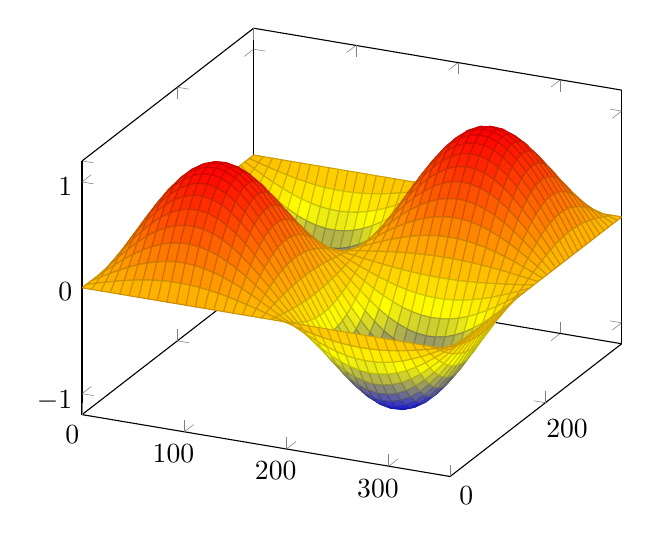
\begin{tikzpicture}
\begin{axis}
\addplot3[
surf,
domain=0:360,
samples=40,
] {sin(x)*sin(y)};
\end{axis}
\end{tikzpicture}
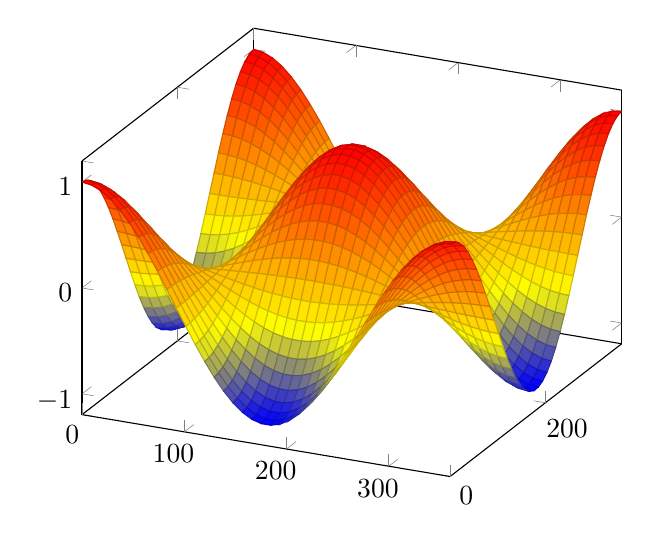
\begin{tikzpicture}
\begin{axis}
\addplot3[
surf,
domain=0:360,
samples=40,
] {cos(x)*cos(y)};
\end{axis}
\end{tikzpicture}

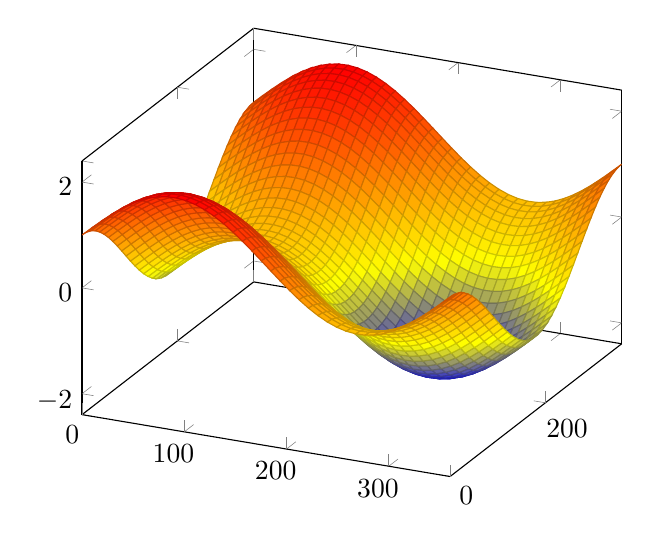
\begin{tikzpicture}
\begin{axis}
\addplot3[
surf,
domain=0:360,
samples=40,
] {sin(x)+cos(y)};
\end{axis}
\end{tikzpicture}
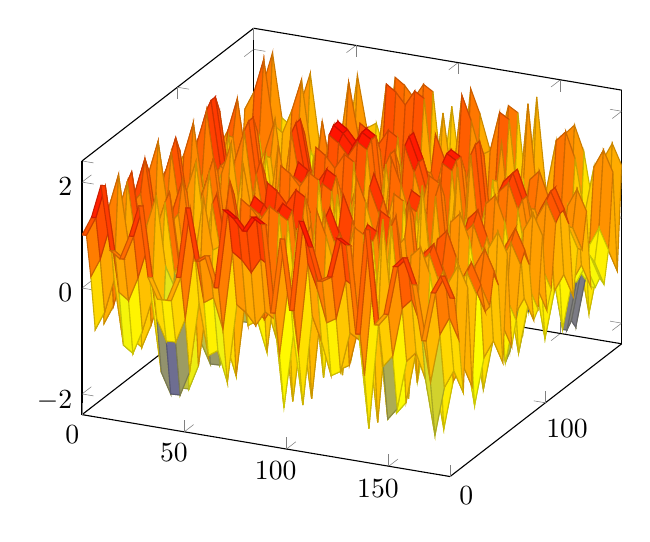
\begin{tikzpicture}
\begin{axis}
\addplot3[
surf,
domain=0:180,
samples=40,
] {sin(x*x)+cos(y*y)};
\end{axis}
\end{tikzpicture}

\begin{tikzpicture}
\begin{axis}
\addplot gnuplot [
id=sin,
] {sin(x)};
\end{axis}
\end{tikzpicture}


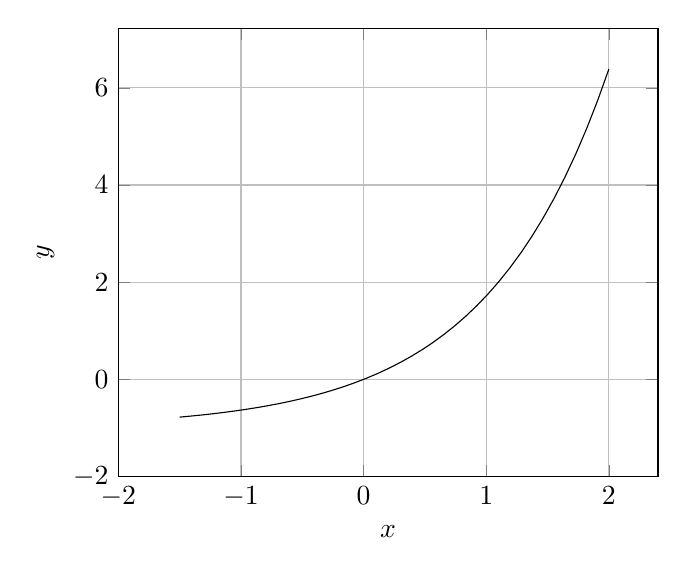
\begin{tikzpicture}
\begin{axis}[
xmin=-2,
ymin=-2,
xlabel= $x$,
ylabel= $y$,
grid=major,
]
\addplot[
domain=-1.5:2,
samples=40,
] {e^x-1};
\end{axis}
\end{tikzpicture}

\begin{tikzpicture}
\begin{axis}[
axis line=center,
xmin=-5.5,
ymin=-4,
xlabel= $x$,x label style={right},
ylabel= $y$,y label style= {above},
grid=major,
]
\addplot[
domain=-5.5:3,
samples=100,
] {1+x+x^2/2+x^3/6+x^4/24};
\end{axis}
\end{tikzpicture}


\begin{tikzpicture}
\datavisualization [school book axes, visualize as smooth line]
data [format=function] {
var x : interval [-1.3:1.3];
func y = \value x*\value x*\value x;
};
\end{tikzpicture}


\section{Symbols, Shortcuts and Semantic Aliasing}

Although Journals recommend not to alias LaTeX commands the harsh reality is that each topic and paper has different needs for notations and things can get messy.

Consider papers written for computations of floating algorithms. We might find in preambles definitions like, 
{\parskip0pt\large
\begin{verbatim}
%% Floating-point machine operations.
\newcommand{\mop}{\boxcircle}
\newcommand{\madd}{\boxplus}
\newcommand{\msub}{\boxminus}
\newcommand{\mmul}{\boxdot}
\newcommand{\mdiv}{\boxdiag}
\end{verbatim}
}
\newcommand{\mop}{\boxcircle}
\newcommand{\madd}{\boxplus}
\newcommand{\msub}{\boxminus}
\newcommand{\mmul}{\boxdot}
\newcommand{\mdiv}{\boxdiag}

I consider aliasing of non-semantic commands to semantic commands, such as the machine operation |\mop| from |\boxcircle| as good practice. 

\begin{texexample}{Example with macro aliasing}{ex;aliasing}
\begin{Definition} \summary{(Absorption.)}
Let $x, y, z \in \Fset$ with $y, z \in \Rset$,
let $\mathord{\mop}$ be any IEEE~754 floating-point operator,
and let $x = y \mop z$.
Then $y \mop z$ gives rise to \emph{absorption} if
\begin{itemize}
\item
$\mathord{\mop} = \mathord{\madd}$
and either $x = y$ and $z \neq 0$, or $x = z$ and $y \neq 0$;
\item
$\mathord{\mop} = \mathord{\msub}$
and either $x = y$ and $z \neq 0$, or $x = -z$ and $y \neq 0$;
\item
$\mathord{\mop} = \mathord{\mmul}$
and either $x = \pm y$ and $z \neq \pm 1$, or $x = \pm z$ and $y \neq \pm 1$;
\item
$\mathord{\mop} = \mathord{\mdiv}$,
$x = \pm y$ and $z \neq \pm 1$.
\end{itemize}
\end{Definition}
\end{texexample}


The most obvious shortcuts should be for calligraphic or fraktur math alphabets.


\begin{texexample}{Calligraphic Alphabet}{ex:callalphabet}
\providecommand*{\cA}{\ensuremath{\mathcal{A}}}
\providecommand*{\cB}{\ensuremath{\mathcal{B}}}
\providecommand*{\cC}{\ensuremath{\mathcal{C}}}
\providecommand*{\cD}{\ensuremath{\mathcal{D}}}
\providecommand*{\cE}{\ensuremath{\mathcal{E}}}
\providecommand*{\cF}{\ensuremath{\mathcal{F}}}
\providecommand*{\cG}{\ensuremath{\mathcal{G}}}
\providecommand*{\cH}{\ensuremath{\mathcal{H}}}
\providecommand*{\cI}{\ensuremath{\mathcal{I}}}
\providecommand*{\cJ}{\ensuremath{\mathcal{J}}}
\providecommand*{\cK}{\ensuremath{\mathcal{K}}}
\providecommand*{\cL}{\ensuremath{\mathcal{L}}}
\providecommand*{\cM}{\ensuremath{\mathcal{M}}}
\providecommand*{\cN}{\ensuremath{\mathcal{N}}}
\providecommand*{\cO}{\ensuremath{\mathcal{O}}}
\providecommand*{\cP}{\ensuremath{\mathcal{P}}}
\providecommand*{\cQ}{\ensuremath{\mathcal{Q}}}
\providecommand*{\cR}{\ensuremath{\mathcal{R}}}
\providecommand*{\cS}{\ensuremath{\mathcal{S}}}
\providecommand*{\cT}{\ensuremath{\mathcal{T}}}
\providecommand*{\cU}{\ensuremath{\mathcal{U}}}
\providecommand*{\cV}{\ensuremath{\mathcal{V}}}
\providecommand*{\cW}{\ensuremath{\mathcal{W}}}
\providecommand*{\cX}{\ensuremath{\mathcal{X}}}
\providecommand*{\cY}{\ensuremath{\mathcal{Y}}}
\providecommand*{\cZ}{\ensuremath{\mathcal{Z}}}
\begin{luacode}
local alphabet = {"A","B","C","D","E","F","G","H","I","J","K","L",
                  "M","N","O","P","Q","R","S","T","U",
                  "V","W","X","Y","Z"}
for k,v in pairs(alphabet) do
	tex.print("\\c"..v..", ")
end
\end{luacode}
\end{texexample}


\section{Calculus}



\subsection*{Differentiation}
Leibnitz invented the transmutation theorem for finding the area under a curve. Finding areas beneath curves
was 


\subsection*{Integration}

\subsection*{Limits}

\marginpar{\includegraphics[width=3cm]{bolzano}
{\scriptsize\RaggedLeft Bolzano begins his work by explaining what he means by theory of science, and the relation between our knowledge, truths and sciences. Human knowledge, he states, is made of all truths (or true propositions) that men know or have known. This is, however, only a very small fraction of all the truths that exist, although still too much for one human being to comprehend. Therefore, our knowledge is divided into more accessible parts. Such a collection of truths is what Bolzano calls a science (Wissenschaft). It is important to note that not all true propositions of a science have to be known to men; hence, this is how we can make discoveries in a science.}}

\textbf{Bolzano} Although implicit in the development of calculus of the 17th and 18th centuries, the modern idea of the limit of a function goes back to Bolzano who, in 1817, introduced the basics of the epsilon-delta technique to define continuous functions. However, his work was not known during his lifetime.\footcite{coolidge} The first publication in English had to wait for almost 150 years and it was published by Coolidge in 1949 in his popular work \emph{The Mathematetics of Great Amateurs.} Grattan-Guiness\footcite{grattan-guiness} falls short though of accusing Cauchy of plagiarizing the work of Bolzano and other contemporaries.


\textbf{Cauchy} discussed variable quantities, infinitesimals, and limits and defined continuity of {$\displaystyle y=f(x)$} $y=f(x)$ by saying that an infinitesimal change in $x$ necessarily produces an infinitesimal change in $y$ in his 1821 book \emph{Cours d'analyse}, while (Grabiner 1983) claims that he only gave a verbal definition. 

\textbf{Weierstrass} first introduced the epsilon-delta definition of limit in the form it is usually written today. He also introduced the notations $\lim$ and $\lim x\rightarrow x_0$. The notation which has been used widely at the time in Europe was
$\operatorname{Lim}_{x=a}$, to express the \enquote{the limit as $x$ approaches $a$.} It is found in papers of Weierstrass, who in 1841 wrote $\lim$ and in 1854 \enquote{$\underset{n=\infty}{\operatorname{Lim.}}\:p_n = \infty $}

In later publications we find $\operatorname{Lim}$ without the point, but still capitalized. I particularly like the way the equations were grouped and the limit indicated by cases and shown in fig.~\ref{weis}.

\begin{figure}[htbp]
\centering
\includegraphics[width=0.8\textwidth]{weistrass}
\caption{Extract from Weierstrass publication.}
\label{weis}

\end{figure}

To create a new operator symbol we can use \cs{operatorname}. The command will take care of spacing, whereas if we use only
|\mathrm| it will not. If we were to use it frequently we could also define a macro using \cs{DeclareMathOperator} from amsmath. 

\begin{texexample}{operatorname}{ex:onames}

$$\operatorname{Lim.}p_n$$

$$\operatorname{Lim}.p_n$$

$$\mathrm{Lim.}p_n$$ 
\end{texexample}

By the early 1900's the notation started approaching more to what is commonly used in today's publications.

\textbf{Hardy} The modern notation of placing the arrow below the limit symbol is due to Hardy in his book \emph{A Course of Pure Mathematics} in 1908, however in the preface to the book he credits Leathem and Bromwich\footcite{bromwich}.\footnote{Hardy wrote ... there are two respects in which I have diverted ...} 


\begin{gather}
\begin{aligned}
f(a) &= f\left[\lim_{k\rightarrow\infty} x_k \right]=\lim_{k} f(x_k)\le 0 & \text{ and }\\
f(a) &= f\left[\lim_{k\rightarrow\infty} X_k \right]=\lim_{k} f(X_k)\ge 0. & \\  
\end{aligned}
\end{gather}

In Cauchy's words, these inequalities established that ``the quantity
$f(a)$ \ldots cannot differ from zero.'' He had thus proved the existence of a
number a between $x$ and $X$ for which $f(a) = O$. The general version of the
intermediate value theorem, namely that a continuous function takes all
values between $f(x_0)$ and $f(X)$, follows as an easy corollary.
This was a remarkable achievement. Cauchy had, for the most part,
succeeded in demonstrating a "self-evident" principle by analytic methods.


Apart from open intervals, limits can be defined for functions on arbitrary subsets of R, as follows.  Let $f$ be a real-valued function defined on a subset $S$ of the real line.  Let $p$ be a limit point of ''S'' that is, ''p'' is the limit of some sequence of elements of ''S'' distinct from p.  The limit of ''f'', as ''x'' approaches ''p'' from values in ''S'', is ''L'' if, for every {{nowrap|''ε'' > ''0''}}, there exists a δ > ''0'' such that {{nowrap|0 < {{abs|''x'' − ''p''}} < ''δ''}} and {{nowrap|''x'' ∈ ''S''}} implies {{nowrap|{{abs|''f''(''x'') − ''L''}} < $\epsilon$.

This limit is often written

\[
L = \underset{x\in S}{\lim_{x\to p}} f(x).
\]

The condition that $f$ be defined on $S$ is that $S$ be a subset of the domain of $f$.  This generalization includes as special cases limits on an interval, as well as left-handed limits of real-valued functions (e.g., by taking ''S'' to be an open interval of the form $(-\infty,a)$, and right-handed limits (e.g., by taking ''S'' to be an open interval of the form $(a,\infty)$. It also extends the notion of one-sided limits to the included endpoints of (half-)closed intervals, so the Square root function $f(x)=\sqrt{x}$ can have limit 0 as $x$ approaches 0 from above.




\section*{Fraktur letters}

Individual Fraktur letters are sometimes used in mathematics, which often denotes associated or parallel concepts by the same letter in different fonts. For example, a Lie group is often denoted by ''G'', while its associated Lie algebra is $\mathfrak{g}$. 
A ring ideal might be denoted by $\mathfrak{a}$ (or $\mathfrak{p}$ if a prime ideal) while an element is $a \in \mathfrak{a}$. The Fraktur $\mathfrak c$ is also sometimes used to denote the cardinality of the continuum, that is, the cardinality of the real line. In model theory, $\mathfrak{A}$ is used to denote an arbitrary model, with ''A'' as its universe. Fraktur is also used in other ways at the discretion of the author.


\begin{luacode}
local alphabet = {"A","B","C","D","E","F","G","H","I","J","K","L",
                  "M","N","O","P","Q","R","S","T","U","V","W","X","Y","Z"}
for k,v in pairs(alphabet) do
	tex.print("\\mathfrak{"..v.."}, ")
end
\end{luacode}

Special symbols such as dingbats loaded using the \pkg{pifont} package need to be enclosed within an \docAuxCommand{mbox} in order to be able to display the glyph properly.
\bigskip

\begin{texexample}{Using special dingbat symbols}{}
\label{e14}
 We start by showing that the function $f(x)=x^2$ is
continuous over the set $X_2$\label{p:X2} defined as the interval
$[0,1]$ where numerals $\frac{i}{\mbox{\ding{172}}}, 0 \le i \le
\mbox{\ding{172}},$ are used to express its points in units $\mu$.
First of all, note that the set $X_2$ is continuous in   $\mu$
because its points are equidistant with the distance
$d=\mbox{\ding{172}}^{-1}$. Since this function is strictly
increasing,  to show its continuity it is sufficient to check the
difference $f(x)-f(x^{-})$ at the point $x=1$. In this case,
$x^{-}=1-\mbox{\ding{172}}^{-1}$ and we have
\[
 f(1)-f(1-\mbox{\ding{172}}^{-1})=
 1-(1-\mbox{\ding{172}}^{-1})^2 =
 2\mbox{\ding{172}}^{-1}(-1)\mbox{\ding{172}}^{-2}.
\]
This number is infinitesimal, thus $f(x)=x^2$ is continuous over
the set $X_2$. \hfill $\Box$
\end{texexample}

\cs{Box}
Notice the use of the \docAuxCommand{Box} command to draw a square for  end of proof symbol. This is from the amsmath package. The box is placed at the end of the line using |\hfill $\Box$|.

%
%\begin{Rule}
%Alias common symbols to semantic macro names that follow their mathematical definitions.
%\end{Rule}
%
%\begin{Rule}
%Create shorcut commands with moderation for alphabets and algebras and alias if necessary. Good practice, sets etc.
%\end{Rule}



\section{Partial derivatives}

Partial derivatives can be typeset using the \latex{} command \cs{partial}

\begin{texexample}{Partial Derivatives}{ex:partial}
\[
dS = \frac{\partial S}{\partial x}\, dx
   + \frac{\partial S}{\partial y}\, dy
   = \left(y - \frac{2V}{x^2}\right) dx
   + \left(x - \frac{2V}{y^2}\right) dy.
\]
\meaning\partial
\end{texexample}


This is using a certain style. For other styles it maybe more difficult.

\section*{Binomial Coefficients}

To typeset binomial coefficients or similar structures, use the command
\cs{binom} from \pkg{amsmath}\index{amsmath>binom}

\begin{texexample}{Binomial}{ex:binomial0}
\[
\begin{align}
(x+y)^3 & = x^3 + 3x^2y + 3xy^2 + y^3, \\[8pt]
(x+y)^4 & = x^4 + 4x^3y + 6x^2y^2 + 4xy^3 + y^4, \\[8pt]
(x+y)^5 & = x^5 + 5x^4y + 10x^3y^2 + 10x^2y^3 + 5xy^4 + y^5, \\[8pt]
(x+y)^6 & = x^6 + 6x^5y + 15x^4y^2 + 20x^3y^3 + 15x^2y^4 + 6xy^5 + y^6, \\[8pt]
(x+y)^7 & = x^7 + 7x^6y + 21x^5y^2 + 35x^4y^3 + 35x^3y^4 + 21x^2y^5 + 7xy^6 + y^7.
\end{align}
\]
\end{texexample}


Pascal's rule can be typeset as:


\begin{texexample}{Binomial Distribution}{ex:binomial}
\[
\binom{n}{k} =\binom{n-1}{k}
+ \binom{n-1}{k-1}
\]
\end{texexample}



\section[Symbols and Abbreviations]{Symbols and Abreviations}
\label{math:abbreviations}

\label{abbr}\label{symbols}%

\begin{texexample}{Creating symbols}{ex:parallelogram}
\newlength{\dentwidth}\setlength{\dentwidth}{\textwidth}
\addtolength{\dentwidth}{-\parindent}

\makeatletter
\gdef\@parallelogram#1{%
  \textnormal{\setbox\z@\hbox{#1/}\dimen@\wd\z@
   \@tempdima 2.45\dimen@
   \vbox{\offinterlineskip
      \hbox{\kern.8\dimen@\vrule\@width\@tempdima\@height.4\p@}%
      \kern-.0\p@
      \hbox to\@tempdima{#1/\hfil\rlap/}%
      \kern-.5\p@
      \hbox{\kern.1\dimen@\vrule\@width\@tempdima\@height.4\p@}}}}
      
 \gdef\Par{%
   \mathchoice
      {\@parallelogram\scriptsize}%
      {\@parallelogram\scriptsize}%
      {\@parallelogram\tiny}%
      {\@parallelogram\tiny}}

            



\begin{tabular*}{\dentwidth}{rl@{\extracolsep{\fill}}l@{\extracolsep{0pt}}@{\dots}l}

$>$ & is (or are) greater than. & Def. & definition. \\
$<$ & is (or are) less than. & Ax. & axiom. \\
$\Bumpeq$ & is (or are) equivalent to. & Hyp. & hypothesis. \\
$\therefore$ & therefore. & Cor. & corollary. \\
$\perp$ & perpendicular. & Scho. & scholium. \\
$\perp_s$ & perpendiculars. & Ex. & exercise. \\
$\parallel$ & parallel.\qquad $\parallel_s$ parallels. & Adj. & adjacent. \\
$\angle$ & angle.\qquad $\angle_s$ angles. & Iden. & identical. \\
$\triangle$ & triangle.\qquad $\triangle_s$ triangles. & Const. & construction. \\
$\Par$ & parallelogram. & Sup. & supplementary. \\
$\Par_s$ & parallelograms. & Ext. & exterior. \\
$\odot$ & circle.\qquad $\odot_s$ circles. & Int. & interior. \\
rt. & right.\qquad  st.\ straight. & Alt. & alternate. \\
\end{tabular*}


\hbox{\qed\ stands for quod erat demonstrandum, \emph{which was to be proved}.\hss}

\newcommand{\qef}{\textsc{q.e.f.}}
\qef\ stands for quod erat faciendum, \emph{which was to be done.}

The signs $+$, $-$, $\times$, $\div$, $=$, have the same meaning as in Algebra.

\makeatother   
\end{texexample}
   
\section{Afixing symbols to other symbols}

\latex provides \docAuxCommand{stackrel} for placing a superscript above a binary relation. In the \pkg{amsmath} package there are somewhat more general commands \docAuxCommand{overset} and \docAuxCommand{underset}, that can be used to place one symbol above or below another symbol, whether is a relation or something else. Oberdiek's package \pkg{stackrel}\footcite{stackrel} extends the syntax by adding an optional argument for the subscript position. It follows the syntax of extensible arrows of the packages |amsmath| and |mathtools|.

\begin{docCommand}{stackrel}{\oarg{subscript}\marg{superscript}{\marg{rel}}}
  Typeset a subscript or superscript above a symbol.
\end{docCommand}

\ifSTACKREL
\begin{texexample}{Example of stackrel and stackbin}{ex:stackrel}
\[
 A \stackbin[\text{and}]{}{+} B \stackrel[x]{!}{=} C
\] 
\end{texexample}
\else
\begin{texcode}{Example of \cs{stackrel} and \cs{stackbin}}{ex:stackrel}
  Example cannot be shown as the package stackrel is not loaded.
\end{texcode}
\fi


\chapter{Matrices and Mathematical Environments}
\label{matrices}

\section{Matrices}

Matrices have a long history of application in solving linear equations but they were known as arrays until the 1800s. The Chinese text The Nine Chapters on the Mathematical Art written in 10th–2nd century BCE is the first example of the use of array methods to solve simultaneous equations,[102] including the concept of determinants. In 1545 Italian mathematician Gerolamo Cardano brought the method to Europe when he published Ars Magna.[103] The Japanese mathematician Seki used the same array methods to solve simultaneous equations in 1683.[104] 


The Dutch statesman and mathematician Johan (Jan) de Witt represented transformations resembling arrays in his 1659 book Elements of Curves (1659). He is also perhaps the second Mathematician to be lynched\footnote{Hypatia, was torn to bits by a lynching Christian mob in the streets of Alexandria in \textsc{AD} 415.} by a mob and had parts of their bodies eaten! [\ldots]The brothers were shot and then left to the mob. Their naked, mutilated bodies were strung up on the nearby public gibbet, while the Orangist mob partook of their roasted livers in a cannibalistic frenzy. Throughout it all, a remarkable discipline was maintained by the mob, according to contemporary observers, making one doubt the spontaneity of the event.\footcite{israel1995} \textit{Elementa Curvarum Linearum} has been described as the first textbook in analytic geometry.\footnote{The savage murder of a man that history has judged a highly competent leader is regarded by the Dutch as one of the most shameful episodes in their history.}


Between 1700 and 1710 Gottfried Wilhelm Leibniz publicized the use of arrays for recording information or solutions and experimented with over 50 different systems of arrays.[103] Cramer presented his rule in 1750.

The term "matrix" (Latin for "womb", derived from mater—mother[106]) was coined by James Joseph Sylvester in 1850,[107] who understood a matrix as an object giving rise to a number of determinants today called minors, that is to say, determinants of smaller matrices that derive from the original one by removing columns and rows. In an 1851 paper, Sylvester explains:

\begin{quote}
I have in previous papers defined a \enquote{Matrix} as a rectangular array of terms, out of which different systems of determinants may be engendered as from the womb of a common parent.[108]
\end{quote}

Arthur Cayley published a treatise on geometric transformations using matrices that were not rotated versions of the coefficients being investigated as had previously been done. Instead he defined operations such as addition, subtraction, multiplication, and division as transformations of those matrices and showed the associative and distributive properties held true. Cayley investigated and demonstrated the non-commutative property of matrix multiplication as well as the commutative property of matrix addition.[103] Early matrix theory had limited the use of arrays almost exclusively to determinants and Arthur Cayley's abstract matrix operations were revolutionary. He was instrumental in proposing a matrix concept independent of equation systems. In 1858 Cayley published his A memoir on the theory of matrices[109][110] in which he proposed and demonstrated the Cayley–Hamilton theorem.[103] Cayley introduced a particular notation for fencing the array as shown in fig~\ref{fig:cayley}, which used () for the first row and $\vert$ for subsequent rows.

\begin{figure}[htbp]
\centering
\includegraphics[width=0.6\textwidth]{cayley-notation}

\caption{Extract from Caley's paper \textit{A memoir on the theory of matrices.}}
\label{fig:cayley}

\end{figure}

An English mathematician named Cullis was the first to use modern bracket notation for matrices in 1913 and he simultaneously demonstrated the first significant use of the notation $A = [a_{i,j}]$ to represent a matrix where $a_{i,j}$ refers to the i$^$th row and the $j$th column.

Cayley's introductory paper in matrix theory was written in French and published in a German periodical. In this paper, matrices are introduced to simplify the notation which arises in simultaneous linear equations.  

\begin{gather}
\begin{aligned}
\xi  &= \alpha x + \beta y + \gamma z + \dots\\
\eta  &= \alpha' x + \beta' y + \gamma' z + \dots\\
\zeta &= \alpha'' x + \beta'' y + \gamma'' z + \dots
\end{aligned}
\end{gather}

The set of equations is written as:

\begin{gather}
(\xi, \eta, \zeta,\dots ) = (\alpha,\beta,\gamma,\dots)(x,y,z,\dots)
\end{gather}

The same article also introduces, although quite sketchily, the ideas of inverse matrix and of matrix multiplication, or \enquote{compounding} as Cayley called it. The above basic properties are expanded in a second expository article\footcite{fieldman1962} which
also lists many additional properties of matrices. In this important paper, Cayley works mostly with square matrices with
nine elements. He represents the zero matrix,\footcite[This is an interesting development]{fieldman1962}

\[
\begin{vmatrix}
0,0,0\\
0,0,0\\
0,0,0
\end{vmatrix}
\]
by \enquote{0} and the \enquote{matrix unity,}

\[
\begin{vmatrix}
1,0,0\\
0,1,0\\
0,0,1
\end{vmatrix}
\]
by \enquote{1}

Caley then introduces the algebra of matrices by defining the addition of two matrices by

\begin{gather}
(\begin{cayleymatrix}{3}
a&b&c\\
a' &b' & c'\\
a''&b'' & c''\\
a''' & b''' & c'''\\
\end{cayleymatrix}) +
(\begin{cayleymatrix}{3}
\alpha & \beta & \gamma\\
\alpha & \beta & \gamma\\
\alpha & \beta & \gamma\\
\end{cayleymatrix})\:\: = \:\:
(\begin{cayleymatrix}{3}
a+a  &b+b  &c+\gamma\\
a''+\alpha' & b'' + \beta'' & c'' +\gamma'' \\
a'''+\alpha''' & b''' + \beta''' & c''' +\gamma''' \\
\end{cayleymatrix})
\end{gather}
Caley stated but without proof, that matrices are commutative and associative under addition. Two types
of multiplication are exhibited. The first type is designated as \enquote{scalar multiplication,} that is

\[
m(\begin{cayleymatrix}{3}
a & b & c\\
a' & b' & c'\\
a'' & b'' & c''
\end{cayleymatrix}) 
= 
(\begin{cayleymatrix}{3}
ma & mb & mc\\
ma' & mb' & mc'\\
ma'' & mb'' & mc''
\end{cayleymatrix})
\]

The notation used for the matrix (\begin{cayleymatrix}{3}
a&b\\
c&d\\
e&f
\end{cayleymatrix}) is defined later on. It is a special environment.

The second type of multiplication is called \enquote{compounding,} according to the following scheme:

\begin{multline}
(\begin{cayleymatrix}{3}
a  &b &c\\
a' &b' &c'\\
a'' &b'' &c''
\end{cayleymatrix}\between \begin{cayleymatrix}{3}
\alpha & \beta & \gamma\\
\alpha'' & \beta'' & \gamma''\\
\alpha'' & \beta'' & \gamma''\\
\end{cayleymatrix})
\\=
 (\begin{cayleymatrix}{3} \bigl(a,b,c\between a, a',a''\bigr) & (a,b,c\between (\beta, \beta', \beta'') & (a,b,c\between \gamma, \gamma', \gamma'')\\
(a &b &c\\
(a &b &c
\end{cayleymatrix})\label{caleyprod}
\end{multline}

The product equation is complex to type, but very clear to understand its definition.\footnote{Uses multline environment.}


Later developments are described by Feldmann\footcite[This is the second paper that appeared in the \textit{The Mathematics Teacher relating to matrices.}][]{feldmann1963}. 

In the 1930s books on matrices written in English started to appear. The two leading ones were C.C. MacDuffee \textit{Theory of Matrices,} Springer (1933) and J. H. M. Wedderburn \textit{Lectures on Matrices}\footnote{The book was published by the American Mathematical Society and bears reseblance to a publication printed using TeX.} (1934). They both wrote matrices with double vertical lines as in

\[
\begin{Vmatrix}
a_{11} & a_{12} & \dots & a_{1n}\\
a_{11} & a_{12} & \dots & a_{1n}\\
\vdots & \vdots & \vdots & \vdots\\
a_{n1} & a_{n2} & \dots &a_{nn}
\end{Vmatrix}
\]
The use of double vertical lines was easy to typeset as well as to handwrite. It could also relate to the single vertical lines which are used to denote determinants.




%%%%%%%%%%%%%%%%%%%%%%%%%%%%%%%%%%%%%%%%%%%%%
%%%%%%%%  TYPOGRAPHY %%%%%%%%%%%%%%%%%%%%%%%%
\section{Typography of Matrices}

Matrices are mostly typed the way tabular environements are types, i.e., you need to use the tabulator sign ``\&''.
Mathematical environments are provided both by \latexe as well as amsmath. The latter are to be preferred.

\begin{docEnvironment}{array}{\marg{specifier}}
\end{docEnvironment}

The |array| environment is a \latex2e provided environment and is identical to tabular, but works automatically with mathematics. It has to be enclosed in a mathematical environment.


\begin{texexample}{Matrices}{ex:matrices}
\[
\mathbf{X} = \left(
\begin{array}{ccc}
x_1 & x_2 & \ldots \\
x_3 & x_4 & \ldots \\
\vdots & \vdots & \ddots
\end{array} \right)
\]
\end{texexample}

\section{AMS Math matrices}

The \pkg{amsmath} package provides environments that go beyond the basic \docAuxEnvironment{array} of \latex2e. The \docAuxEnvironment{pmatrix}, \docAuxEnvironment{Bmatrix}, \docAuxEnvironment{vmatrix} and \docAuxEnvironment{Vmatrix}. 
There is also a \docAuxEnvironment{smallmatrix} that is more suitable for inline text display. 

\begin{texexample}{Using \textbackslash smallmatrix}{ex:smallmatrix}
This is a small matrix $\bigl(\begin{smallmatrix}
a&b\\
c&d\\
\end{smallmatrix}\bigr)$ environment. \lorem
\end{texexample}


\begin{docEnvironment}{bmatrix}{}
The example \ref{ex:bmatrix} illustrates the typesetting of a bracketted matrix hence \ul{b}matrix. If you want the matrix equation to be numbered enclose it withn an |equation| or |gather| environment. In this documentation we have let the |equation| environment to |gather| hence it will make no difference which ever is used. (amsmath)
\end{docEnvironment}

\begin{texexample}{Bmatrix}{ex:bmatrix}
\begin{equation}
\begin{matrix}
1 & 2 \\
3 & 4
\end{matrix} \qquad
\begin{bmatrix}
p_{11} & p_{12} & \ldots & p_{1n} \\
p_{21} & p_{22} & \ldots & p_{2n} \\
\vdots & \vdots & \ddots & \vdots \\
p_{m1} & p_{m2} & \ldots & p_{mn}
\end{bmatrix}
\end{equation}
\end{texexample}

The \refEnv{bmatrix} is from the amsmath package, see also \vref{bmatrix} and \nameref{bmatrix} and \pageref{bmatrix}. 


One issue to be aware is that the \refEnv{bmatrix} does not allow more than 10 tab stops. If you need to use more, you will have to \docCounter{MaxMatrixCols} to a higher number. The |phd| package sets this automatically at 20, so you will not have to worry about it.

\begin{teX}
\setcounter{MaxMatrixCols}{20}
\end{teX}

\begin{texexample}{Large Matrices}{ex:largematrices}
\[
\begin{bmatrix}
1 & 0 & 0 & -1 & 0  & 0  & 1 & -1 & 1  & -1 & 0 \\
0 & 1 & 0 & 0  & -1 & 0  & 1 & -1 & 0  & 1  & -1 \\
0 & 0 & 1 & 0  & 0  & -1 & 1 & -1 & -1 & 0  & 1 
\end{bmatrix}
\]
\end{texexample}



\section{vmatrix}

\begin{texexample}{vmatrix}{ex:vmatrix}

\begin{gather}
\begin{vmatrix}
aa' + bb' + cc' & ea' + fb' + gc' \\
ae' + bf' + cg' & ee' + ff' + gg'
\end{vmatrix}
{} = \begin{vmatrix}
a & b \\
e & f
\end{vmatrix}  \begin{vmatrix}
a' & b' \\
e' & f'
\end{vmatrix} + \begin{vmatrix}
a & c \\
e & g
\end{vmatrix}  \begin{vmatrix}
a' & c' \\
e' & g'
\end{vmatrix}.
\end{gather}
\end{texexample}





\section{Single equations that are too long}

In many cases equations need to be written over two or more lines. The \pkgname{amsmath} package, provides environments that are suitable for this:


\begin{texexample}{The multiline amsmath environment}{ex:multiline}
\begin{multline}
   a + b + c + d + e + f+ g + h + i  + k + l + m + n + o + p\\
              = j + k + l + m + n +\cos^{2}-1
\end{multline}
\end{texexample}



\section{array environment}

This is simply the same as the |eqnarray| environment only with the possibility of
variable rows and columns and the fact, that the whole formula has only one
equation number and that the array environment can only be part of another math
environment, like the equation environment or the displaymath environment. With
@{} before the first and after the last column the additional space |\arraycolsep| is
not used, which maybe important when using left aligned equations.

\begin{texexample}{array environment}{ex:array2}
\begin{eqnarray}
  a & = & b + c \\
    & = & d + e + f + g + h + i
               + j + k + l \nonumber \\
    &   & +\: m + n + o \\
    & = & p + q + r + s
\end{eqnarray}
\end{texexample}

The equations
to be aligned are entered with each one terminated by \cs{cr}. In each equation there should be
one alignment symbol \& to indicate where the alignment should take place. This is usually
done at the equal signs, although it is not necessary to do so. For example


\begin{texexample}{The array environment}{ex:array}
Thus to change $\frac34$ to a decimal divide $4$ into $3$
and we get $.75$ as a result, thus:
\[
\begin{array}{r@{}r@{}}
4 \; & \vline \; 3.00 \\\cline{2-2}
     &            .75
\end{array}
\]

To find the square root of a four-figure number
such as our example calls for, work it out in the
following manner:
\[
\arraycolsep=0em
\begin{array}{cccccccccccc}
\multicolumn{3}{c}{\text{2d pair}} &\qquad&\qquad&
\multicolumn{3}{c}{\text{1st pair}}&\qquad&\qquad&
\multicolumn{2}{c}{\text{square root}}\\
 & \overbrace{\quad}&\ZZZ&&&\ZZZ&\overbrace{\quad}&\ZZZ\\
 & 42 &&&&& 25 &&&&\vline\;65&(answer)\\\cline{11-11}
 & 36 &&&&& \\\cline{2-2}
\multirow{2}{*}{125\:} & \vline\hfill \Zi6 \hfill&&&&& 25\\
 & \vline\hfill \Zi6 \hfill&&&&& 25\\\cline{2-7}
\end{array}
\]
\end{texexample}


\subsection{Array environment in game theory}

This example \ref{ex:gamearray} is from \footnote{From determinacy to Nash equilibrium,St\'ephane Le Roux, TU Darmstadt }

\begin{texexample}{array environment in game theory}{ex:gamearray}
The game $\langle\{a,b,c\},\{1,2,3,4\}^3,\{0,1,2,3,4\},v,(<_d)_{d\in\{a,b,c\}}
\rangle$ is represented below, where player $a$ chooses the row, $b$ the column, and $c$ the array. 
\[\begin{array}{c@{\hspace{1cm}}c@{\hspace{1cm}}c@{\hspace{1cm}}c}
\begin{array}{|c|c|c|c|}
\hline 1 & 1 & 1 & 1\\
\hline 1 & 1 & 1 & 1\\
\hline 1 & 1 & 1 & 1\\
\hline 4 & 1 & 1 & 1\\
\hline
\end{array}
&
\begin{array}{|c|c|c|c|}
\hline 1 & 2 & 1 & 1\\
\hline 2 & 2 & 2 & 2\\
\hline 1 & 2 & 1 & 1\\
\hline 4 & 2 & 1 & 1\\
\hline
\end{array}
&
\begin{array}{|c|c|c|c|}
\hline 1 & 1 & 3 & 1\\
\hline 1 & 1 & 3 & 1\\
\hline 3 & 3 & 3 & 3\\
\hline 4 & 1 & 3 & 1\\
\hline
\end{array}
&
\begin{array}{|c|c|c|c|}
\hline 2 & 4 & 4 & 4\\
\hline 4 & 3 & 4 & 4\\
\hline 4 & 4 & 4 & 4\\
\hline 0 & 0 & 0 & 0\\
\hline
\end{array}
\end{array}
\]
Let us show that the game $\langle\{a,b,c\},\{1,\dots,n\}^3,\{0,\dots,n\},v,(<_d)_{d\in\{a,b,c\}}
\rangle$ witnesses the claim. First, the preferences are linear orders indeed. Second, let us show that there is no Nash equilibrium by case-splitting below. 
\end{texexample}



\section{The AMSmath Package}

\index{maths environment>align}
\index{maths environment>align}
\index{maths environments}{falign}
\index{maths environments}{xalignat}
\index{maths environments}{xxalignat}
\index{maths environments}{eqnarray}

The \pkg{amsmath} package offers five different align environments, |align|, |alignat|, |falign|, |xalignat| and |xxalignat|. 

In difference to the \refEnv{eqnarray} environment from standard \latex the ``three'' parts of one equation expr.-symbol-expr. are divided by only one ampersand in two parts. In general the ampersand should be before the symbol to get the right spacing, for example y \&= x. 

\subsection{The align environment}

The |align| environment is considered an improvement over \latex's |eqnarray| environment. It is very similar to a tabular
environment and is aligned at the |&|. 
It requires one |&| less and produces a tighter equation. Mathematicians 
are very particular in not using |eqnarray| and the package 
\pkgname{onlyamsomath} if used will warn if it finds that it has been used in the document. 
\index{eqnarray (environment)>spacing}
\index{eqnarray (environment)>alternatives}
\index{math environments>align}
\index{math environmenta>eqnarray}


\begin{texexample}{Comparison between |align| and |eqnarray|}{ex:eqnarraycomp}
% First example with eqnarray
\begin{eqnarray}
a & = & b + c \\
  & = & d + e + f + g + h + i
        + j + k + l \nonumber \\
  &   & +\: m + n + o \\
  & = & p + q + r + s
\end{eqnarray}

% Second example with align
\begin{align}
a & =  b + c \\
  & =  d + e + f + g + h + i
       + j + k + l \nonumber \\
  & +\: m + n + o \\
  & =  p + q + r + s
\end{align}
\end{texexample}


You can observe in Example~\ref{eqnarraycomp} the essential differences between the two, which we re-iterate, it requires one less |&| and produces a tighter display.

\begin{texexample}{The align environment}{ex:align}
\begin{align}
         y & = d\label{eq:IntoSection}\\
         y & = cx+d\\
    y_{12} & = bx^{2}+cx+d\\
     y(x)  & = ax^{3}+bx^{2}+cx+d
 \end{align}

%\begin{align*}
%\therefore (13 - x_1) + (13 - x_2) + \dotsb + (13 - x_p) + r &= 52\,,\\
%\therefore 13p - (x_1 + x_2 + \dotsb + x_p) + r              &= 52\,,\\
%\therefore x_1 + x_2 + \dotsb + x_p                          &= 13p - 52 + r\\
%                                                          &= 13 (p - 4) + r\,.
%\end{align*}

whence we conclude that $\gamma$ is a primitive root modulo $p$. But
\begin{align*}
\gamma^{p-1}-1 &=
     g^{p-1} - 1 + \frac{p-1}{1!}g^{p-2}xp +
        \frac{(p-1)(p-2)}{2!}g^{p-3}x^2p^2 + \ldots \\
  &= p\left(kp + \frac{p-1}{1!}g^{p-2}x +
        \frac{(p-1)(p-2)}{2!}g^{p-3}x^2p + \ldots\right).
\end{align*}
\end{texexample}

As you can observe from example\ref{ex:align}, each line is numbered if the unstarred version of the command is used. The |aligned| environment remedies this.
 


\subsection{The aligned environment}

The aligned environment allows more than one horizontal alignment but has only one equation number.

%\newcommand{\dotsbsmall}{\ldot\!\ldot\!\ldot}
%\newcommand{\ldot}{\mathbin{.}}			% dot with math spacing
%\newcommand{\nobf}[1]{\no \textbf{#1}}		% no with bold number
%
%\begin{texexample}{aligned environment example}{}
%\begin{equation}
%\begin{aligned}
%  &\:C_1x^{r_1}\,[\varphi_{r_1 0} \,+ \varphi_{r_1 1}\log x \,+ \dotsb + \varphi_{r_1 \alpha_1}(\log x)^{\alpha_1}]\\
%+ &\:C_2x^{r_2}\,[\varphi_{r_2 0} \,+ \varphi_{r_2 1}\log x \,+ \dotsb + \varphi_{r_2 \alpha_2}(\log x)^{\alpha_2}]\\
%+ &\multispan{1}{\:\dotfill}\\
%+ &\:C_nx^{r_n}[\varphi_{r_n 0} + \varphi_{r_n 1}\log x + \dotsb + \varphi_{r_n \alpha_n}(\log x)^{\alpha_n}],
%\end{aligned}
%\end{equation}
%
%\[
%\tag{98}
%\left\{\qquad
%\begin{aligned}
%T_1 &= T_2 = T_3 (=T)\\
%p_1 &= p_2 = p_3\\
%s_1-s_2 &= \frac{(u_1-u_2)+p_1(v_1-v_2)}{T}\\
%s_2-s_3 &= \frac{(u_2-u_3)+p_2(v_2-v_3)}{T}.
%\end{aligned}
%\right.
%\]
%\end{texexample}
 




\subsection{How to interrupt a display}

\begin{docCommand}{intertext}{}
 In many instances you will want to interrupt a display with some text. This can be accomplished using the control sequence |\intertext|.
 \end{docCommand}
 
 

\begin{texexample}{Using \cs{intertext}}{ex:intertext}
\begin{gather}
\begin{aligned}
U &= M u = M(c_v T + b)\\
S &= M(c_v  \log T + \frac{R}{m}  \log v + a),\\
\intertext{and } 
F &= M \left\{T(c_v - a - c_v \log T) - \frac{RT}{m} \log v + b \right\}.
\end{aligned}
\end{gather}
\end{texexample}

As the command \docAuxCommand{intertext} can only come after a |\\|  command we place it accordingly at {1}. Its function is to preserve the alignment after the text is typeset. This is a common requirement in many mathematical 
structures and the command can be used in all of amsmath aligning environments.







\subsection{The alignat environment}

\begin{docEnvironment}{alignat}{}
The alignat environment means \emph{align at} and can be used to align a set of equations vertically at more than one place. The star version of the environment omits the equation numbering.
\end{docEnvironment}


%\begin{texexample}{The alignat environment}{}
%\renewcommand{\dotsb}{\ldots}			% use lower dots after +-
%\renewcommand{\dotsbsmall}{\ldot\!\ldot\!\ldot}
%\renewcommand{\ldot}{\mathbin{.}}			% dot with math spacing
%\renewcommand{\nobf}[1]{\no \textbf{#1}}	
%
%\begin{alignat*}{5}
%  &p_{i+1}\dfrac{d^{m-i-1}y_1}{dx^{m-i-1}} &&+ \dotsbsmall +p_{m}y_1
%  && = -\Big(\dfrac{d^{m}y_1}{dx^{m}} &&+p_1\dfrac{d^{m-1}y_1}{dx^{m-1}}
%  &&+ \dotsbsmall +p_{i}\dfrac{d^{m-i}y_1}{dx^{m-i}}\Big), \\
%\multispan{10}{\makebox[36em]{\dotfill},}\\
% &p_{i+1}\dfrac{d^{m-i-1}y_{m-i}}{dx^{m-i-1}} &&+ \dotsbsmall +p_{m}y_{m-i}\!
% &&= -\Big(\dfrac{d^{m}y_{m-i}}{dx^{m}} &&+ p_1\dfrac{d^{m-1}y_{m-i}}{dx^{m-1}}
% &&+ \dotsbsmall +p_{i}\dfrac{d^{m-i}y_{m-i}}{dx^{m-i}}\Big).
%\end{alignat*}
%\end{texexample}



Remember that when using one of the align environments, there should be no |\\| at the end of the
last line, otherwise you will get another equation number for this ``empty''  line.


\subsection{Multline}

\begin{docEnvironment}{multline}{\meta{contents}}
\end{docEnvironment}
The |multline| environment is another attempt at displaying long equations. It will set the first line flush left and the last one flush right. It can be quite useful when one has very long equations. The line break is marked with |\\|. It is good typographical practice to have the first line shorter than the last line and not the other way around.

\begin{texexample}{Multiline Equations}{mult}
Example unumbered
\begin{multline*}
x^{\rho}f(x, \rho) = x^{\rho} \Big [ u_{m}x^{m}\frac{\rho(\rho-1)\ldots (\rho-m+1)}{x^{m}} \\
                   + u_{m-1}x^{m-1}\frac{\rho(\rho-1)\ldots (\rho-m+2)}{x^{m-1}}+ \ldots
                   + u_{2}x^{2}\frac{\rho(\rho-1)}{x^2}+u_{1}x\frac{\rho}{x}+u_0 \Big ].
\end{multline*}
Example  numbered
\begin{multline}
M \left[\delta u - \left(T_1\, \frac{dp_{12}}{dT_{12}} - p_1\right) \delta v\right] \\
= \delta T_{12} \left[M_{12}\, \frac{du_{12}}{dT_{12}} + M_{21}\, \frac{du_{21}}{dT_{12}}
  - \left(T_1\, \frac{dp_{12}}{dT_{12}} - p_1\right)
    \left(M_{12}\, \frac{dv_{12}}{dT_{12}}
        + M_{21}\, \frac{dv_{21}}{dT_{12}}\right)\right].
\end{multline}
\end{texexample}



\section{gathered}

The |gathered| environment is like the |aligned| or |alignat| environment. They use
only so much horizontal space as the widest line needs. In difference to the gather
environment it must be itself inside math mode.

\begin{docEnvironment}{gathered}{\meta{contents}}
\end{docEnvironment}

\emphasize{cases}
\begin{texexample}{The gathered environment}{exe:gathered}
\[
  \left .
   \begin{gathered}
    \left [ \frac{\alpha}{p} \right ] +
    \left [ \frac{\alpha}{p^2} \right ] +
    \left [ \frac{\alpha}{p^3} \right ] +
    \ldots \\
    \left [ \frac{\beta}{p} \right ] +
    \left [ \frac{\beta}{p^2} \right ] +
    \left [ \frac{\beta}{p^3} \right ] +
    \ldots \\
      \vdots \\
    \left [ \frac{\lambda}{p} \right ] +
    \left [ \frac{\lambda}{p^2} \right ] +
    \left [ \frac{\lambda}{p^3} \right ] +
    \ldots
   \end{gathered}
  \right \} \tag{B}
\]
\end{texexample}

\section{The cases environment}

The \refEnv{cases} environment renders multiple lines with an extensible left curly-brace. It can be used for piecewise-defined functions. For this to work, you must have |\usepackage{amsmath}| in the preamble.

\newlength{\boxla}
\newlength{\boxlb}
\newlength{\boxlc}
\setlength{\boxla}{1.15in}
\setlength{\boxlb}{1.7in}
\setlength{\boxlc}{1.6in}
\newcommand{\boxa}[1]{\makebox[\boxla]{\small #1\dotfill}}
\newcommand{\boxb}[1]{\makebox[\boxlb]{\small #1\dotfill}}

\begin{docEnvironment}{cases}{}
\end{docEnvironment}


\begin{texexample}{The cases environment}{ex:cases}
\begin{align*}
\boxa{DOYEN} & \quad
\parbox{3.4in}{\small MM. \\
MILNE EDWARDS, Professeur. Zoologie, Anatomie, \\
\hspace*{1.5in} Physiologie compare.}
\\
\parbox[b]{\boxla}{\small PROFESSEURS\\HONORAIRES\dotfill} &
\begin{cases}
\text{\small DUMAS.}\\
\text{\small PASTEUR.}
\end{cases}
\\
\boxa{PROFESSEURS} &
\begin{cases}
\boxb{CHASLES}\text{\small Gomtrie suprieure.} \\
\boxb{P. DESAINS}\text{\small Physique.} \\
\boxb{PUISEUX}\text{\small Astronomie.} \\
\boxb{JAMIN}\text{\small Physique.} \\
\boxb{O. BONNET}\text{\small Astronomie.}
\end{cases}
\\
\boxa{AGROGES} &
\begin{cases}
\parbox{\boxlb}{%
\small BERTRAND\dotfill\\
J. VIEILLE\dotfill}\bigg\} \text{\small Sciences mathematiques.} \\
\boxb{PELIGOT}\text{\small Sciences physiques.}
\end{cases}\\
\boxa{SECRETAIRE} & \quad \text{\small PHILIPPON.}
\end{align*}
\end{texexample}


\begin{texexample}{}{}
non plus orthogonale mais telle que
\[
{\sum_{i}}' a_{pi} a_{qi}
  = \begin{cases}
    0 & \text{ si } p \gtrless q \\
    1 & \text{ si } p = q
    \end{cases}
\]
alors on a aussi
\[
{\sum_{i}}' a_{pi} a_{iq}
  = \begin{cases}
    0 & \text{ si } p \gtrless q \\
    1 & \text{ si } p = q
    \end{cases}
\]
\end{texexample}



\section{flalign}

\emphasize{falign}
\begin{docEnvironment}{falign}{\meta{contents}}
\end{docEnvironment}

%\cxset{
%         tag left bracket =[,
%         tag right bracket =],
%         tag font-weight=\textbf,
%      } 
%\newtagform{squarebrackets}{[}{]}
%\usetagform{squarebrackets}

\begin{texexample}{flalign}{ex:flalign}
\begin{flalign}
&&
\chi\omega  &= \omega - S \omega\, \nabla \centerdot \sigma\, dt, &&\\
&\text{whence}&
\chi'^{-1} \omega &= \omega + \nabla_1 S \omega \sigma_1\, dt, &&
\end{flalign}
\end{texexample}
%\newtagform{roundbrackets}{(}{)}
%\usetagform{roundbrackets}



\section{Sums}

\newcommand\reverseprop{\rotatebox[origin=c]{180}{$\propto$}}

Of the various special kinds of numbers used in analysis, there is hardly a species that 
that is so important and so generally applicable as the Bernoulli  
Numbers. Their numerous properties and applications have caused the creation 
of an extensive literature on the subject which still continues to attract the 
attention of scholars. The first statement of the properties of these numbers 
was given to the world by their inventor Jacques (1) Bernoulli (1654-1705) in 
his posthumously printed work, \emph{Ars Conjectandi} (Basel, 1713), pages 95 to 
98. 

Earlier scholars produced similar results the most important being Faulhaber and Remmelin of Ulm, Wallis, Mercator, in his \emph{Logarithmotechnia} and others.

Bernoulli's original notation is unfamiliar to modern mathematics. He used three notations, first the
summation symbol he used was $\smallint$ which followed Leibnitz. He also used 2 dots to indicate 
grouping. For \ldots he use an {\panunicode Ӿ}  with a bar in the middle. 
Note that Bernoulli writes $n.n-1$ where we would write $n(n-1)$. he also uses Descartes equality symbol, which in our modern notation is a mirrored proportionality symbol \(\reverseprop\) that indicates the equal sign.%
\footnote{This equality symbol was widely used in France and Holland during the latter part of the seventeeth and early eighteenth centuries, but it never attained a substantial foothold in other countries.} His use of $nn$ instead of $n^2$ should also be noted.

\def\xellipsis{\begingroup\mkern\thinmuskip \mbox{\panunicode Ӿ}\mkern\thinmuskip\endgroup}
\begin{longtable}{lll}
\smallint    & |\smallint| & Summation (modern notation  $\sum$)\\
\reverseprop & |\reverseprop| & Equality sign i.e, $=$\\
$\xellipsis$   & |\xellipsis|   & Ellipsis i.e., \ldots\\
  $n.n$        & |n.n-1|          & brackets $n(n-1)$\\
\end{longtable}

\[\smallint \overline{n-1}\]



\[\frac{n.n-1}{1.2} = \frac{nn-n}{2}\]

{\def\arraystretch{1.5}
\setlength\arraysep{3.5pt}
\begin{align}
\smallint\! n   = & \frac{1}{2}nn + \frac{1}{2}n,\\
\smallint\! nn  = & \frac{1}{3}n^3 + \frac{1}{2} nn + \frac{1}{6}n,\\
\smallint\! n^3 = & \frac{1}{4}n^4 + \frac{1}{2} n^3 + \frac{1}{4}nn,\\
\smallint\! n^4 = & \\
\smallint\! n^5 = & \frac{1}{5}n + \frac{1}{2}n^5 + \frac{5}{12}n^4 \xellipsis - \frac{1}{12}nn\\
\smallint\! n^6 = & \\
\smallint\! n^7 = & \\
\smallint\! n^8 = & \\
\smallint\! n^9 = & \\
\smallint\! n^{10} =& \frac{1}{11}n^{11} + \frac{1}{2}n^{10}+\frac{5}{6}n^9 \xellipsis -1n^7 \xellipsis 1n^5 \xellipsis -\frac{1}{2}n^3 \xellipsis  \frac{5}{66}n
\end{align}
}



\[a_1 + a_2 + \dots +a_n,\]
where each $a_k$ is a number that has been defined somehow. 
Each element $a_k$ of a sum is called a \emph{term}. 

The threedots notation has many uses, but it can be ambiguous and a bit long-winded. Another alternative, is the delimited form.

\begin{gather}
\sum_{k=1}^n a_k,
\end{gather}
which is called the Sigma-notation because it uses the upper case Greek letter sigma $\Sigma$.



\begin{equation*}
P = \frac{\displaystyle{
\sum_{i=1}^n (x_i- x)
(y_i- y)}}
{\displaystyle{\left[
\sum_{i=1}^n(x_i-x)^2
\sum_{i=1}^n(y_i- y)^2
\right]^{1/2}}}
\end{equation*}


\section{Math accents}

Mathematical accents are a bit different that the ones used for normal text in order to cater, firstly for the exotic taste in diagritics taste by mathematicians and secondly to cater for the fact that mathematics is styled in italics.
This is a short summary of what is available. 
\bigskip

%\begin{tabular}{llllll}
%\toprule
%$\hat{a}$    & \docCommand{hat\{a\}} & $\check{a}$ & \docCommand{check\{a\}} &$\tilde{a}$&\docCommand{tilde\{a\}}\\
%$\grave{a}$ &\docCommand{grave\{a\}}    & $\dot{a}$ &\docCommand{dot\{a\}} &$\ddot{a}$ &\docCommand{ddot\{a\}}\\
% $\bar{a}$ &\docCommand{bar\{a\}} & $\vec{a}$ &\docCommand{vec\{a\}} & $\widehat{AAA}$ &\docCommand{widehat\{AAA\}}\\
%$\acute{a}$ &\docCommand{acute\{a\}} &$\breve{a}$  &\docCommand{breve\{a\}} &$\widetilde{AAA}$ &\docCommand{widetilde\{AAA\}}\\
% & & & & &\\%CHEXK mathring gives problems
%\bottomrule
%\end{tabular}

\section{Binary Relations}


%\begin{tabular}{llllll}
%\toprule
%$<$ &$<$  &$>$ &$>$ &$=$ &$=$\\
%$\le$  &\docCommand{leq} or \docCommand{le}  &$\geq$ &\docCommand{geq} or \docCommand{ge} &$\equiv$ &\docCommand{equiv}\\
%$\ll$  &\docCommand{ll}   &$\gg$  &\docCommand{gg}   &$\doteq$  &\docCommand{doteq} \\
%$\prec$ &\docCommand{prec} &$\succ$  &\docCommand{succ} &$\sim$ &\docCommand{sim}\\
%$\preceq$ &\docCommand{preceq} &$\succeq$  &\docCommand{succeq} &$\simeq$ &\docCommand{simeq}\\
%$\subset$ &\docCommand{subset}  &$\supset$ &\docCommand{supset} &$\approx$ &\docCommand{approx}\\
%$\subseteq$ &\docCommand{subseteq} &$\supseteq$  &\docCommand{supseteq} &$\cong$  &\docCommand{cong} \\
%$\sqsubset$  &\docCommand{sqsubset}  &$\sqsupset$  &\docCommand{sqsupset}  &$\Join$  &\docCommand{Join}\\
%$\sqsubseteq$   &\docCommand{sqsubseteq}   &$\sqsupseteq$ &\docCommand{sqsupseteq}   &$\bowtie$ &\docCommand{bowtie} \\
%$\in$ &\docCommand{in}  &$\ni$ &\docCommand{ni}, \docCommand{owns} &$\propto$ &\docCommand{propto}\\
%$\vdash$ &\docCommand{vdash}  &$\dashv$ &\docCommand{dashv} &$\models$ &\docCommand{models}\\
%
%\bottomrule
%\end{tabular}



\section{Brackets, braces and parentheses}

In addition  to the previous commands \cmd{Bigg} and \cmd{Biggm} can be used to add a bit more horizontal space.

\[3\Big\downarrow 
\Big\Downarrow\]


\[3\Big\updownarrow
\Big\Updownarrow\]

Another way to typeset the big separators is to split them over a line as shown below

{\arraycolsep=2pt
 \begin{equation}
 \begin{array}{rcl}
 \frac{1}{2}\Delta(f_{ij}f^{ij}) & = & 2\Bigg({\displaystyle
 \sum_{i<j}}\chi_{ij}(\sigma_{i}-\sigma_{j})^{2}+f^{ij}%
 \nabla_{j}\nabla_{i}(\Delta f)+\\
 & & +\nabla_{k}f_{ij}\nabla^{k}f^{ij}+f^{ij}f^{k}[2
 \nabla_{i}R_{jk}-\nabla_{k}R_{ij}]\Bigg)
 \end{array}
 \end{equation}

This is achieved by typing

\begin{teX}
{\arraycolsep=2pt
 \begin{equation}
 \begin{array}{rcl}
 \frac{1}{2}\Delta(f_{ij}f^{ij}) & = & 2\Bigg({\displaystyle
 \sum_{i<j}}\chi_{ij}(\sigma_{i}-\sigma_{j})^{2}+f^{ij}%
 \nabla_{j}\nabla_{i}(\Delta f)+\\
 & & +\nabla_{k}f_{ij}\nabla^{k}f^{ij}+f^{ij}f^{k}[2
 \nabla_{i}R_{jk}-\nabla_{k}R_{ij}]\Bigg)
 \end{array}
 \end{equation}

\end{teX}



\chapter{Maths Typography}

\texttt{
Handbook of Typography for the\\
Mathematical Sciences\\
Steven G. Krantz\\
January 21, 2003}\par

\url{http://www.faqorama.net/tecno/[LaTeX]%20Handbook%20of%20Typography%20for%20the%20Mathematical%20Sciences%20-%20S.G.Krantz%20(2003).pdf}


Ellen Swanson’s book Mathematics into Type is a unique and important contribution to the literature of technical typesetting. It set a
standard for how mathematics should be translated from a handwritten
manuscript to a printed book or document. While Swanson’s book was
intended primarily as a resource for technical typesetters, it was also important to mathematical and other technical authors who wanted to take
an active role in ensuring that their work reached print in an attractive
and accurate form.
The landscape has now changed considerably. With the advent and
wide availability of \tex,
most mathematicians can take a more active
role in producing typeset versions of their work. Indeed, many mathematicians currently use TEX to write preliminary versions of their work
that are very similar (in many respects) to what will ultimately appear
in print.

While the output from \tex has a more typeset appearance than that
from most word processors, the TEX product is not automatically (without human intervention) \enquote{ready to go to press}. There are still \enquote{post processing} typesetting issues that must be addressed before a work
actually appears in print. 

The style and format of running heads, section headings and other titles, the formatting of theorems and other
enunciations, the text at the bottom of the page, page break issues, and
the fonts and spacing used in all of these go under the name of “page design”. These are often customized for a particular book or journal. The
index and table of contents must be designed and typeset. Graphics,
and sometimes new fonts, must be integrated. Additional questions of
style in the formatting of equations and superscripts and subscripts can
also arise. Most TEX users do not know how to handle the questions just
listed, which is why most publishers currently send \tex documents for
books or journal articles to a third-party \tex consultant. The purpose
of the present work is to serve as a touchstone for those who want to
learn to make typesetting decisions themselves.


\def\smsqr#1#2{\sqrt{{#1}^2 + {#2}^2} + \frac{1}{{#1}^2 + {#2}^2}}

\[ \smsqr{a}{c} \]

There are other aspects of consistency about which many authors
are blissfully unaware: spacing above and below a displayed equation,
spacing above and below a theorem,6
space after a proof, the mark at
the end of a proof (QED, or the Halmos "tombstone" |\qed|, for example).\footnote{ "The symbol is definitely not my invention — it appeared in popular magazines (not mathematical ones) before I adopted it, but, once again, I seem to have introduced it into mathematics. It is the symbol that sometimes looks like \(\boxed{\thinspace}\), and is used to indicate an end, usually the end of a proof. It is most frequently called the 'tombstone', but at least one generous author referred to it as the 'halmos'.", Paul R. Halmos, I Want to Be a Mathematician: An Automathography, 1985, p. 403.}

Again, a good macro can be invaluable in addressing these issues; but
awareness of the problem is also a great asset.

\begin{latexquotation}
You make everyone's
life easier if you eschew the eccentric and stick to the most basic constructions. This advice is valid for the Plain \tex user, for the \latex
user, for the Microsoft Word user, and for every other user of electronic
tools.
\end{latexquotation}



\section{Choose your notation carefully}
\index{maths>typography>notation}

Some believe that mathematics is created others that it is discovered, \emph{notation} is certainly created and
a matter that has occupied the minds of many mathematicians. Peterson\footcite{peterson2009} \footcite{peterson2009}  went as far as to claim  `that notation can direct the course of mathematics’ and perhaps rightly so.

Bad notation can make good exposition bad and bad exposition worse; ad hoc decisions about notation, made mid-sentence in the heat of composition, are almost certain to result in bad notation. Good notation has a kind of alphabetical harmony and avoids dissonance.

Leibniz had a lading role in the development of mathematical notations. He made a prolonged study of matters of notation: 
(538)

Leonhard Euler was one of the most prolific mathematicians in history, and also a prolific inventor of canonical notation. His contributions include his use of e to represent the base of natural logarithms. It is not known exactly why {$\displaystyle e$} e was chosen, but it was probably because the four letters of the alphabet were already commonly used to represent variables and other constants. Euler used {$\displaystyle \pi$ }  to represent pi consistently. The use of {$\displaystyle \pi$ }   was suggested by William Jones, who used it as shorthand for perimeter. Euler used {$\displaystyle i$}  to represent the square root of negative one,[note 41] although he earlier used it as an infinite number. [note 42][note 43] For summation, Euler used sigma, Σ.[note 44] For functions, Euler used the notation {$\displaystyle f(x)$}  to represent a function of {$\displaystyle x$} . In 1730, Euler wrote the gamma function.[note 45] In 1736, Euler produces his paper on the Seven Bridges of Königsberg[72] initiating the study of graph theory.


\begin{figure}[htbp]
\includegraphics[width=\textwidth]{shot8}
\caption{The equation of love from \emph{Rites of Love and Math}. The equation which has been shown as a tatoo  on Kayshonne Insixieng May, first appeared in a 100-page paper \emph{Instantons Beyond Topological Theory I} \cite{frenkel2012,FLN}}
\end{figure}


\subsection{One symbol, one letter}
\index{maths>typography>symbols}

A mathematical symbol is usually indicated by \emph{one} letter, not two or three. If for example we want to suggest that the \textit{factor of safety} is equal to three, we should write
\[F_{\mathrm{s}}=3\]
and not
\[F_{\mathrm{safetyfactor}}=3\]
or worse
\[F_{\mathrm{sf}}=3\]
typesetting the subscript in \textit{italic} font is also wrong
\[F_{s}=3\]
as it does not represent a mathematical symbol, but is just an abbreviation for safety factor.

Sometimes the use of the one symbol one letter rule cannot be applied, without the notation becoming complex
\medskip

{
\narrower\narrower
The static friction force \(F_{\mathrm{sf}}\) will exactly oppose forces applied to an object parallel to a surface contact up to the limit specified by the [[coefficient of static friction]] \(\mu_{\mathrm{sf}}\) multiplied by the normal force \(F_N\). In other words the magnitude of the static friction force satisfies the inequality:

\[ \le F_{\mathrm{sf}} \le \mu_{\mathrm{sf}} F_\mathrm{N}. \]

The kinetic friction force \(F_{\mathrm{kf}}\) is independent of both the forces applied and the movement of the object. Thus, the magnitude of the force equals:

\[F_{\mathrm{kf}} = \mu_{\mathrm{kf}} F_\mathrm{N}\]

where \(\mu_{\mathrm{kf}}\) is the coefficient of kinetic friction.
}




\newthought{Do not start a sentence with an equation}

\newthought{Display math}

In general mathematics typeset better when they are displayed. Use in-line maths only for the simplest of equations and for explanations of symbols and the like. Watch out for inconsistent spacing before and after displayed math.

\subsection{Correct badly sized math}

Briggs worked out the table from scratch. Starting with $\log 10 = 1$, he calculated
successively $\sqrt{10}$, $\sqrt{\sqrt{10}}$, $\sqrt{\sqrt{\sqrt{10}}}$, $\cramped{\sqrt{\sqrt{\sqrt{\sqrt{10}}}}}$ \ldots , until after 54 such root extractions he reached a number very close to 1.


$\sqrtsign{a12}$

\meaning\sqrtsign


\begin{quote}
The 2005 Euro\TeX{} ... 16th ($\cramped{2^{2^2}}$)($2^{2^2}$) ...
\end{quote}

Some \tex constructions typeset rather badly, consider for example this:

\[
\sqrt{\frac{\beta}{\gamma}} = \sqrt{X} + \sqrt{y}
\]

\noindent or this,

\[
\surd{\frac{\beta}{\gamma}} = \surd{X} + \surd{y}
\]


You can remedy this by using a \cs{mathstrut}.


\begin{texexample} {Correcting square roots} {ex:sqroot}
\[
\sqrt{\mathstrut a}=\sqrt{\mathstrut X}+\sqrt{\mathstrut y}
\sqrt{\mathstrut a}=\sqrt{\mathstrut X}+\sqrt{\mathstrut y_{i,j}}
\]
\end{texexample}



\newthought{Multiplication}

One of the most common errors is to use the ``dot'' to indicate multiplication between scalars\footnote{\url{http://www.tug.org/TUGboat/Articles/tb29-2/tb92guiggiani.pdf}}. For example the folowing formul\ae
\[a\cdot x^2+b\cdot x+c=0\]
should be written as
\[ax^2+bx+c=0\]

In fact, for the the sake of simplicity, the standard multiplication between letters, or between letters, or between a number and a letter, does not require any symbol. If, on the other hand, the multiplication is between two numbers, the $\times$ or $\cdot$ symbols are required to avoid ambiguity.
For example you should write

\[2\times 3=6 \text{ and not } 2\thickspace 3=6 \]


\paragraph{Using the right font}

Matching the text font with the mathematical font is the job of the class and
style designer. Ideally these should be selected by a specialist at the publisher.

This is now complicated a bit in that there are a limited number of unicode fonts, as well as unicode defined symbols. Nevertheless at least the \docFont{stix} family of fonts is a good start.

The Euler equation involves the five most important mathematical constants. First we typeset it with no space corrections\footnote{\texttt{\textbackslash eu\^\,\{\textbackslash iu\textbackslash pi\}}},
% The number `e'
\providecommand*{\eu}%
{\ensuremath{\mathrm{e}}}
% The imaginary unit
\providecommand*{\iu}%
{\ensuremath{\mathrm{j}}}
\[\scalebox{3}{$\eu^{\iu\pi}$}\]
a small correction to the space should be added

\[\scalebox{3}{$\eu^{\,\iu\pi}$}\]

\subsection{Differential operators}
A peculiar defnition is required to properly
write the differential symbol. It is in fact an operator that has a space only on its left. In Beccari (2007b) the following solution is proposed:

\bigskip


\clearpage
\section{tikz}
\begin{texexample}{Using TikZ with Maths}{ex:tikzmaths}
because of the periodicity of the Jacobi theta functions involved in the construction of the vectors.
The height difference between starting point and endpoint of the path is thus $Lp$ as shown in figure \ref{fig:path}. Moreover, because of the periodicity of the theta functions it is sufficient to restrict the initial height to $\ell_1=0,1,\dots,L-1$ in this case.

{  \centering
  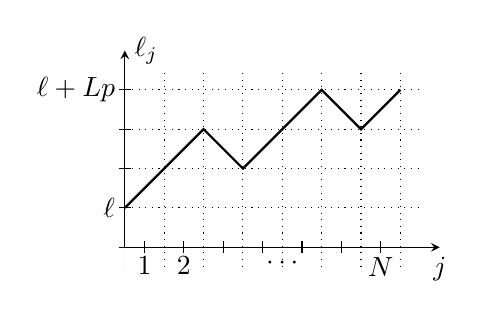
\begin{tikzpicture}[>=stealth]
     \draw[scale=0.5,thick] (0,0)--(2,2)--(3,1)--(5,3)--(6,2)--(7,3);
           
     \draw[<->] (0,2) -- (0,-0.5) -- (4,-0.5);
     \foreach \x in {0.25,0.75,...,3.25}
       \draw[xshift=\x cm,yshift=-0.5cm] (0,-0.075)--(0,0.075);
     
    \foreach \y in {-0.5,0,...,1.5}
       \draw[yshift=\y cm] (-0.075,0)--(0.075,0);
 
    \draw (0.25,-0.5) node[below] {$1$};
    \draw (0.75,-0.5) node[below] {$2$};
    \draw (2,-0.5) node[below] {$\cdots$};
    \draw (3.25,-0.5) node[below] {$N$};
    \draw (4,-0.5) node[below] {$j$};
    \draw (0,0) node [left] {$\ell$};
    \draw (0,1.5) node [left] {$\ell+Lp$};
    \draw (0,2) node [right] {$\ell_j$};
    \clip[scale=0.5] (0,-1.5) rectangle (7.5,3.5);
    \draw[scale=0.5,dotted] (-1,-2) grid (8,5);
  \end{tikzpicture}
}
  
\end{texexample}




%\begin{texexample}{Example}{}
%\newcommand{\ud}{\ensuremath \mathop{}\!\mathrm{d}}
%\(z=2\sin x\mathrm{d}x\) and \(z=2\sin x\ud x\)
%
%
%\newcommand{\ud}{\mathop{}\!\mathrm{d}}
%\bigskip
%
%It uses an empty operator and eliminates the space
%on its left with |\!|.
%
%Note the difference between
%
%\[z=2\sin x\mathrm{d}x  \]
%
%\[z=2\sin x\ud x\]
%
%where the diffrential is obtained respectively with
%|\mathrm{d}| and |\ud|.
%\end{texexample}




\subsubsection{God is in the details}

Sometimes you will be faced with small decisions for which the Journal style manual might not have an answer for you or the journal Editor might have a different opinion to yours. One such question is if one needs to insert the thousand separator in coefficients.

\[
\operatorname{erf}^{-1}(z)=\tfrac{1}{2}\sqrt{\pi}\left (z+\frac{\pi}{12}z^3+\frac{7\pi^2}{480}z^5+\frac{127\pi^3}{40320}z^7+\frac{4369\pi^4}{5806080}z^9+\frac{34807\pi^5}{182476800}z^{11}+\cdots\right )
\]


\[
\operatorname{erf}^{-1}(z)=\tfrac{1}{2}\sqrt{\pi}\left (z+\frac{\pi}{12}z^3+\frac{7\pi^2}{480}z^5+\frac{127\pi^3}{40,320}z^7+\frac{4,369\pi^4}{5,806,080}z^9+\frac{34,807\pi^5}{182{,}476,800}z^{11}+\cdots\right )
\]

\[
\operatorname{erf}^{-1}(z)=\tfrac{1}{2}\sqrt{\pi}\left (z+\frac{\pi}{12}z^3+\frac{7\pi^2}{480}z^5+\frac{127\pi^3}{40{,}320}z^7+\frac{4{,}369\pi^4}{5{,}806{,}080}z^9+\frac{34{,}807\pi^5}{182{,}476{,}800}z^{11}+\cdots\right )
\]



\[
\operatorname{erf}^{-1}(z)=\tfrac{1}{2}\sqrt{\pi}\left (z+\frac{\pi}{12}z^3+\frac{7\pi^2}{480}z^5+\frac{127\pi^3}{40\thinspace 320}z^7+\frac{4\thinspace 369\pi^4}{5\thinspace 806\thinspace 080}z^9+\frac{34\thinspace 807\pi^5}{182\thinspace 476\thinspace 800}z^{11}+\cdots\right )
\]


If you type the commas watch out to put them in |{,}| otherwise \tex's algorithm will leave a space. See the difference below:

\[182{,}476{,}800 \]
\[182,476,800\]

It is interesting to note that Knuth believes that in equations this is unnecessary.
He is quoted in Typesetting Mathematics.


\begin{quotation}
But where Don wrote 1000000 they substituted
1,000,000. Don objected that although this might be justifed in text, his use is perfectly OK in a formula. Well then, they replied, write \(10^6\).
Fine, said, Don, but what do I do 
when the number is 1234567? The IEEE standard here is to insert spaces, thus: 1 234 567.
Don doesn't like this in formulae, but agrees that it may be useful in a high precision context, such as numerical tables. 
\end{quotation}



The following are extracts from his paper \textit{Johann Faulhaber and Sums of Powers}:\footnote{\url{http://www-cs-faculty.stanford.edu/~uno/papers/jfsp.tex.gz}}

{
\[\vcenter{\halign{$#$\hfil\ &$#$\hfil\cr
\Sigma n^{11}&=39916800{n+6\choose 12}+
19958400{n+5\choose 10}+3160080{n+4\choose 8}
+168960{n+3\choose 6}\cr
\noalign{\smallskip}
&\qquad\null+2046{n+2\choose 4}+{n+1\choose 2}\,;\cr
\noalign{\smallskip}
\Sigma n^{13}&=6227020800{n+7\choose 14}+3632428800{n+6\choose 12}+
726485760{n+5\choose 10}\cr
\noalign{\smallskip}
&\qquad\null+57657600{n+4\choose 8}
+1561560{n+3\choose 6}+8190{n+2\choose 4}+\binom{n+1}{2}\,.\cr}}\]
}

Also, note in the last equation the use of a period at the end. 
This is something that evokes strong opinions and flaming wars in fora. 
I am not too sure if I agree on the last one, but the way that Knuth writes 
is very clear and his equations in a way are paragraphs. 
In this case the use of a period is recommended.


\subsection{Punctuation}
\index{maths>typography>punctuation}

There are two schools of thought when it comes to punctuation, that is punctuation in display style formulae. Some authors (Beccari, 2007) argue it is not necessary, others that it is necessary and essential \footcite{guiggiani2008}. Mermin \footcite{mermin89} strongly argued in his third rule that:  `The
Math Is Prose rule simply says: End
a displayed equation with a punctuation
mark. It is implicit in this
statement that the absence of a punctuation
mark is itself a degenerate
form of punctuation that, like periods,
commas or semicolons, can be used
provided it makes sense.''

The authors of this article believe that equations, both in display and text style, are part of the argumentation
and so punctuation should be used to help the reader. An example of good use of punctuation is:


Since
\[ a=b \]
and
\[ b=c,\]
it is proven that
\[ a =c. \]

It is extremely unusual to find an equation end with a question mark but here is one. What is 
\[ a = d^2\mathrm{?} \]

If you do put a question mark or an exclamation mark and you are using unicode fonts,
you will need to use |\mathrm{?}| not to confuse it with the relevant symbols.

Most journals require that equations be punctuated, like normal text. Even if the author of the manuscript disagrees, probably the journal editor will add the punctuation.

Read your mathematical text aloud and introduce punctuation as if it was spelled in words rather than mathematical symbols. 

\subsection{Numbering Equations}
\index{maths>typography>equation numbering}

One question that you may face is the numbering of display equations. Early books used numbering sparingly, whereas many authors go overboard and number all the equations.

According to Knuth et al:\footnote{\url{http://tex.loria.fr/typographie/mathwriting.pdf}}
Numbering all displayed formulas is usually a bad idea; number the important ones only.

Halmos\footnote{\url{http://www.math.uh.edu/~tomforde/Books/Halmos-How-To-Write.pdf}} offers pretty much the same good advice,

\begin{latexquotation}
What about ``inequality (*)", or ``equation (7)", or ``formula (iii)"; should all displays be labelled or numbered? My answer is no. Reason: just as you shouldn't mention irrelevant assumptions or name irrelevant concepts, you also shouldn't attach irrelevant labels. Some small part of the reader's attention is attracted to the label, and some small part of his mind will wonder why the label is there. If there is a reason, then the wonder serves a healthy purpose by way of preparation, with no fuss, for a future reference to the same idea; if there is no reason, then the attention and the wonder were wasted.
\end{latexquotation}

Mermin's argues in his Good samaritan Rule: that it is distressing to having to hunt for an equation back in a manuscript for Eq. (2.46) not because your subsequent progress requires
you to inspect it in detail, but merely to find out what it is about so
you may know the principles that go into the construction of Eq. (7.38).
The Good Samaritan rule says: When referring to an equation identify it by
a phrase as well as a number. No compassionate and helpful person
would herald the arrival of Eq. (7.38) by saying "inserting (2.47) and (3.51)
into (5.13)..." when it is possible to say "inserting the form (2.47) of the
electric field $E$ and the Lindhard form (3.51) of the dielectric function $e$ into
the constitutive equation (5.13). To be sure, it's longer this way but much 
clearer\ldots'

For those that want only the equations that are referenced numbered the package \pkgname{autoref} can automate this. This is not included in this package due to conflicts with \pkgname{mathtools} and \pkgname{amsmath}.
\footnote{See also discussion at \protect\url{http://tex.stackexchange.com/questions/29267/which-equations-should-be numbered/49080\#49080}}

Now if you wish to argue about this is fine.

\section{Mathmode}

\tex is in \textit{mathmode} when it is reading mathematics. The |ifmmode| can be used to find out if \tex is in math mode. It denotes the start of an if-then-else control structure that tests whether \tex is currently in either math mode or display math mode. The |\else| part is optional. <TeX code 1> is processed if TeX is in one of the math modes, otherwise it is ignored. 
If the |\else| section is included and TeX is not in one of the math modes then \meta{TeX code 2} is processed; otherwise it is ignored.


\begin{texexample}{Calligraphic fonts}{ex:cal}

\newcommand{\Acal}{\ifmmode \mathcal{Acal} \else \(\mathcal{Acal}\) \fi}
The commandd efines a macro |\Acal| that can be used both in and out of math mode to typeset a calligraphy script A. 

This is a calligraphic {\Acal} or ({\Acal}).
\end{texexample}


\section{Useful packages}

Besides the main packages that we have discussed so far and which should be in everyone's toolbox, there are a number of other packages that you may find useful. One such package is the \pkgname{multienum}, which although not really a packaged specializing in mathematical typesetting, it provides an environment to set multiple equations, as in an exercise or exam.



\subsection{the multienum package}

The \docpkg{multienum} enables  the typestting of multiple equations on one line and numbering them, either with roman, arabic or alpha letters.

\emphasis{usepackage, multienum,begin,end,multienumerate}
\begin{teXXX}
\documentclass{article}
\usepackage{multienum}
\renewcommand{\regularlisti}{\setcounter{multienumi}{0}%
  \renewcommand{\labelenumi}%
  {\addtocounter{multienumi}{1}\alph{multienumi})}}
\begin{document}
\begin{multienumerate}[oddlist]
\mitemxxx{\(x^2 + y^2 = 1\)}{\(a + b = c\)}{\(r-x = y+z\)}
\mitemxxx{\(f - y = z\)}{\(a - b = 2d\)}{\(r+x = 2y-3z\)}
\end{multienumerate}
\end{document}
\end{teXXX}


\begin{multienumerate}[oddlist]
\mitemxxx{\(x^2 + y^2 = 1\)}{\(a + b = c\)}{\(r-x = y+z\)}
\end{multienumerate}
\begin{multienumerate}[evenlist]
\mitemxxx{\(f - y = z\)}{\(a - b = 2d\)}{\(r+x = 2y-3z\)}
\end{multienumerate}


\hrule

\bigskip

We can also enumerate the items using an even-only or odd only
counter.
\subsection*{Answers to Even-Numbered Exercises}
\begin{multienumerate}[evenlist]
\mitemxxxx{Not}{Linear}{Not}{Quadratic}
\mitemxxxo{Not}{Linear}{No; if $x=3$, then $y=-2$.}
\mitemxx{$(x_1,x_2)=(2+\frac{1}{3}t,t)$ or
$(s,3s-6)$}{$(x_1,x_2,x_3)=(2+\frac{5}{2}s-3t,s,t)$}
\mitemx{$(x_1,x_2,x_3,x_4)= (\frac{1}{4}+\frac{5}{4}s+\frac{3}{4}t-u,s,t,u)$
or $(s,t,u,\frac{1}{4}-s+\frac{5}{4}t+\frac{3}{4}u)$}
\mitemxxxx{$(2,-1,3)$}{None}{$(2,1,0,1)$}{$(0,0,0,0)$}
\end{multienumerate}
\bigskip



\newcommand\thecasestudylabel{Case Study}
\newenvironment{casestudy}[2][]{%
   \clearpage\par\leavevmode
   \addcontentsline{toc}{section}{\thecasestudylabel:  #1}
    \topline\vskip1.5pt
   {\noindent\large CASE STUDY\par}\vspace{3.5pt}
   \noindent\textsc{\large#1}\par
   \bigskip
   {#2}
   \medskip
   \topline
}{%
\vfill\bottomline}

\begin{casestudy}[The Riemann hypothesis.]{%
Typeset the text and the equations, shown below. Use a standard minimal to achieve it. Note the fraktur fonts. Text must all be as one paragraph.}

It is well known that the Riemann zeta function $\zeta(s)$ of a complex variable $s=\sigma+it$ is defined by
\[
\zeta(s)=\sum_{n=1}^{\infty}\frac{1}{n^{s}}
\]
for the real part $\mathfrak{R}(s)>1$ and its analytic continuation in the half plane $\sigma>0$ is
\begin{equation}\label{func:zeta}
\zeta(s)=\sum_{n=1}^{N}\frac{1}{n^{s}}-\frac{N^{1-s}}{1-s}-\frac{1}{2}N^{-s}
+s\int_{N}^{\infty}\frac{\frac{1}{2}-\{x\}}{x^{s+1}}dx
\end{equation}
for any integer $N\geq1$ and $\mathfrak{R}(s)>0$.
It extends to an analytic function in the whole complex plane except for having a simple pole at $s=1$. Trivially, $\zeta(-2n)=0$ for all positive integers. All other zeros of the Riemann zeta functions are called its nontrivial zeros.
\bottomline

\begin{teX}
It is well known that the Riemann zeta function $\zeta(s)$ of a complex variable $s=\sigma+it$ is defined by
\[
\zeta(s)=\sum_{n=1}^{\infty}\frac{1}{n^{s}}
\]
for the real part $\mathfrak{R}(s)>1$ and its analytic continuation in the half plane $\sigma>0$ is
\begin{equation}\label{func:zeta}
\zeta(s)=\sum_{n=1}^{N}\frac{1}{n^{s}}-\frac{N^{1-s}}{1-s}-\frac{1}{2}N^{-s}
+s\int_{N}^{\infty}\frac{\frac{1}{2}-\{x\}}{x^{s+1}}dx
\end{equation}
for any integer $N\geq1$ and $\mathfrak{R}(s)>0$.
It extends to an analytic function in the whole complex plane except for having a simple pole at $s=1$. Trivially, $\zeta(-2n)=0$ for all positive integers. All other zeros of the Riemann zeta functions are called its nontrivial zeros.
\end{teX}

Please note that the maths and the text, are typed as a single block. Do not leave any spaces in between. We have used |\mathfrak| for the fraktur font. We have also used $it$ for the imaginary part. This would depend on the style used in your field. 
\end{casestudy}

\clearpage
\section{Gather}

\begin{docEnvironment}{gather}{}
This is like a multi line environment with no special horizontal alignment. All rows
are centered and can have an own equation number:
\end{docEnvironment}

\begin{texexample}{Gather}{ex:gather}
\begingroup
\def\O{\mathcal{O}}
\begin{gather}
 \O,\O(E_4),\O(E_2),\O(H-E_3-E_5),\O(H-E_3),\O(H-E_5),\\ 
\O(2H-E_1-E_3-E_5-E_6),\O(2H-E_1-E_3-E_5),\O(2H-E_3-E_5-E_6).
\end{gather}

So lautet der Beweis des Satzes $2 \times 2 = 4$:
\begin{gather}
(\Omega^{\nu})^{\mu}{}'x = \Omega^{\nu \times \mu}{}'x \text{ Def.}\\
%\begin{split}
\Omega^{2 \times 2}{}'x = (\Omega^{2})^{2}{}'x = (\Omega^{2})^{1 + 1}{}'x = \Omega^{2}{}'\Omega^{2}{}'x = \Omega^{1 + 1}{}'\Omega^{1 + 1}{}'x\nonumber \\
= (\Omega'\Omega)'(\Omega'\Omega)'x = \Omega'\Omega'\Omega'\Omega'x = \Omega^{1 + 1 + 1 + 1}{}'x = \Omega^{4}{}'x.
%\end{split}
\end{gather}


\begin{gather*}
  x = \Omega^{0}{}' x \text{ Def.\ and}\\
  \Omega'\Omega^{\nu}{}'x = \Omega^{\nu+1}{}'x \text{ Def.}
\end{gather*}
\begin{equation}
  x = \Omega^{0}{}' x \text{ Def.\ and}\\
\Omega'\Omega^{\nu}{}'x = \Omega^{\nu+1}{}'x \text{ Def.}
\end{equation}
\endgroup
\end{texexample}


\section{How to number equations either to the left or right?}
\label{eqnochange}

\latexe uses Plain TeX \docAuxCommand{eqno} and \docAuxCommand{leqno} to place the equation number either to the left or the right of the equation. The placement is done automatically and the recommended way is to set this through the documentclass declaration at the start of the document. This can also be set manually later on through the above control sequences, as shown in the Example~\ref{ex:eqno}.

\begin{texexample}{Left or right numbering}{ex:eqno}
\makeatletter
\[ a = b + x^2 \eqno \@eqnnum \]
or at left
\[ a = b + x^2 \leqno \@eqnnum \]
\makeatother
\end{texexample}


%\meaning\text

%\chapter{Unicode Math}
\tcbdocmarginnote{N 29-06-2018}
Unicode contains separate codepoints for most if not all variations of alphabet
shape one may wish to use in mathematical notation. The complete list is shown
in table 5. Some of these have been covered in the previous sections.
The math font switching commands do not nest; therefore if you want sans
serif bold, you must write |\mathbfsf{...}| rather than |\mathbf{\mathsf{...}}|.
This may change in the future.

\section{Unicode maths font setup}

The promise of Unicode is that all symbols and alphabetic variants are in one font. The \pkgname{unicode-math}
maps all the available unicode math characters of a math font to respective \latex commands. If you have patience you can actually input them directly from the keyboard rather than in commands.

The best advice that I can give you is to read the \pkgname{unicode-math} carefully. 

\begin{docCommand} {setmathfont} { \oarg{range=\meta{unicode range}, \meta{font features } } \marg{font name} }
In many cases using one font might not be adequate. Specific Unicode ranges can be assigned to separate fonts.
\end{docCommand}

\subsection{Control over maths alphabets}

\subsection{Math `versions'}

\subsection{Maths input}

\subsection{Math `style'}

\subsubsection{Bold style}

Similar as in the previous section, ISO standards differ somewhat to \tex’s conventions
(and classical typesetting) for ‘boldness’ in mathematics. In the past, it has
been customary to use bold upright letters to denote things like vectors and matrices.


$$\boldsymbol{\omega} \times \mathbf{T} = \mathbf{T'}$$

$$\mathbf{\omega} = {1\over 2}\kappa \mathbf{B} + {1\over 2}(\kappa \mathbf{B} + \tau \mathbf{T}) + {1\over 2}\tau \mathbf{T} = \kappa \mathbf{B} + \tau \mathbf{T}
$$

\[
\mathbf{e} = \frac{\mathbf{A}}{m k} = \frac{1}{m k}(\mathbf{p} \times \mathbf{L})
\]

\subsubsection{Sans serif style}

\subsubsection{Blackboard or double-struck}



\subsubsection{Caligraphic and Script variants}



\section{Growing and non-growing accents}

This are the most problematic with Unicode fonts.

%%%%%%%% INPUT INTEGRAL FILES %%%%%%%%%%
%%%%%%%%%%%%%%%%%%%%%%%%%%%%%%%
 %% Too many errors here need to revisit.
 \subsection{Delimiters}
 \begin{multicols}{2}
% \showmbrace/{002F}{}
% \showlbrace({0028}{}
% \showlbrace[{005B}{}
% \showlbrace\lbrace{007B}{}
% \showmbrace\backslash{005C}{}
% \showrbrace){0029}{}
% \showrbrace]{005D}{}
% \showrbrace\rbrace{007D}{}
% \showlbrace\lceil{2308}{}
% \showlbrace\lfloor{230A}{}
% \showlbrace\lmoustache{23B0}{*}
% \showlbrace\lbrbrak{2772}{*}
% \showlbrace\lBrack{27E6}{*}
% \showlbrace\langle{27E8}{}, \cmd<
% \showlbrace\lAngle{27EA}{*}
% \showlbrace\lgroup{27EE}{*}
% \showlbrace\lBrace{2983}{*}
% \showlbrace\lParen{2985}{*}
% \showrbrace\rceil{2309}{}
 %\showrbrace\rfloor{230B}{}
% \showrbrace\rmoustache{23B1}{*}
% \showrbrace\rbrbrak{2773}{*}
% \showrbrace\rBrack{27E7}{*}
% \showrbrace\rangle{27E9}{}, \cmd>
% \showrbrace\rAngle{27EB}{*}
% \showrbrace\rgroup{27EF}{*}
 %\showrbrace\rBrace{2984}{*}
% \showrbrace\rParen{2986}{*}
 \end{multicols}

 \begin{multicols}{2}
% \showmbrace\vert{007C}{}, \cmd|
 \showmbrace\Vert{2016}{*}, \cmd\|
 \showmbrace\Vvert{2980}{}
 \showmbrace\uparrow{2191}{}
 \showmbrace\downarrow{2193}{}
 \showmbrace\updownarrow{2195}{}
 \showmbrace\Uparrow{21D1}{}
 \showmbrace\Downarrow{21D3}{}
 \showmbrace\Updownarrow{21D5}{}
% \showmbrace\Uuparrow{290A}{*}
% \showmbrace\Ddownarrow{290B}{*}
% \showmbrace\UUparrow{27F0}{*}
% \showmbrace\DDownarrow{27F1}{*}
% \showmbrace\arrowvert{XXXX}{}
% \showmbrace\Arrowvert{XXXX}{}
% \showmbrace\bracevert{XXXX}{*}
 \end{multicols}

 \subsection{Other bracess}
 \begin{multicols}{2}
 \showsymbol\ulcorner{231C}{*}
 \showsymbol\urcorner{231D}{*}
 \showsymbol\llcorner{231E}{*}
 \showsymbol\lrcorner{231F}{*}
 \showsymbol\Lbrbrak{27EC}{*}
 \showsymbol\Rbrbrak{27ED}{*}
 \showsymbol\llparenthesis{2987}{*}
 \showsymbol\rrparenthesis{2988}{*}
 \showsymbol\llangle{2989}{*}
 \showsymbol\rrangle{298A}{*}
 \showsymbol\lbrackubar{298B}{*}
 \showsymbol\rbrackubar{298C}{*}
 \showsymbol\lbrackultick{298D}{*}
 \showsymbol\rbracklrtick{298E}{*}
 \showsymbol\lbracklltick{298F}{*}
 \showsymbol\rbrackurtick{2990}{*}
 \showsymbol\langledot{2991}{*}
 \showsymbol\rangledot{2992}{*}
 \showsymbol\lparenless{2993}{*}
 \showsymbol\rparengtr{2994}{*}
 \showsymbol\Lparengtr{2995}{*}
 \showsymbol\Rparenless{2996}{*}
 \showsymbol\lblkbrbrak{2997}{*}
 \showsymbol\rblkbrbrak{2998}{*}
 \showsymbol\lvzigzag{29D8}{*}
 \showsymbol\rvzigzag{29D9}{*}
 \showsymbol\Lvzigzag{29DA}{*}
 \showsymbol\Rvzigzag{29DB}{*}
 \showsymbol\lcurvyangle{29FC}{*}
 \showsymbol\rcurvyangle{29FD}{*}
 \showsymbol\lbrbrak{2772}{*}
 \showsymbol\rbrbrak{2773}{*}
 \showsymbol\lbag{27C5}{*}
 \showsymbol\rbag{27C6}{*}
 \showsymbol\Lbrbrak{27EC}{*}
 \showsymbol\Rbrbrak{27ED}{*}
 \end{multicols}

 \section{Alphabetics}
 \begin{multicols}{2}
\showsymbolalpha\Gamma{0393}{}
\showsymbolalpha\Delta{0394}{}
\showsymbolalpha\Theta{0398}{}
\showsymbolalpha\Lambda{039B}{}
\showsymbolalpha\Xi{039E}{}
\showsymbolalpha\Pi{03A0}{}
\showsymbolalpha\Sigma{03A3}{}
\showsymbolalpha\Upsilon{03A5}{}
\showsymbolalpha\Phi{03A6}{}
\showsymbolalpha\Psi{03A8}{}
\showsymbolalpha\Omega{03A9}{}
\showsymbolalpha\alpha{03B1}{}
\showsymbolalpha\beta{03B2}{}
\showsymbolalpha\gamma{03B3}{}
\showsymbolalpha\delta{03B4}{}
\showsymbolalpha\epsilon{03B5}{}
\showsymbolalpha\zeta{03B6}{}
\showsymbolalpha\eta{03B7}{}
\showsymbolalpha\theta{03B8}{}
\showsymbolalpha\iota{03B9}{}
\showsymbolalpha\kappa{03BA}{}
\showsymbolalpha\lambda{03BB}{}
\showsymbolalpha\mu{03BC}{}
\showsymbolalpha\nu{03BD}{}
\showsymbolalpha\xi{03BE}{}
\showsymbolalpha\pi{03C0}{}
\showsymbolalpha\rho{03C1}{}
\showsymbolalpha\sigma{03C3}{}
\showsymbolalpha\tau{03C4}{}
\showsymbolalpha\upsilon{03C5}{}
\showsymbolalpha\phi{03D5}{}
\showsymbolalpha\chi{03C7}{}
\showsymbolalpha\psi{03C8}{}
\showsymbolalpha\omega{03C9}{}
\showsymbolalpha\varepsilon{03F5}{}
\showsymbolalpha\vartheta{03D1}{}
\showsymbolalpha\varpi{03D6}{}
\showsymbolalpha\varrho{03F1}{}
\showsymbolalpha\varsigma{03C2}{}
\showsymbolalpha\varphi{03C6}{}
\showsymbolalpha\nabla{2207}{}
\showsymbolalpha\partial{2202}{}
\showsymbolalpha\imath{1D6A4}{}
\showsymbolalpha\jmath{1D6A5}{}
 \end{multicols}
% \subsection{Accents}
 \begin{multicols}{2}
 \showaccent\grave{0300}{}
 \showaccent\acute{0301}{}
 \showaccent\hat{0302}{}
 \showaccent\tilde{0303}{}
 \showaccent\bar{0304}{}
 \showaccent\breve{0306}{}
 \showaccent\dot{0307}{}
 \showaccent\ddot{0308}{}
 \showaccent\ovhook{0309}{}
 \showaccent\mathring{030A}{}
 \showaccent\check{030C}{}
 \showaccent\candra{0310}{}
 \showaccent\oturnedcomma{0312}{}
 \showaccent\ocommatopright{0315}{}
 \showaccent\droang{031A}{}
 \showaccent\leftharpoonaccent{20D0}{}
 \showaccent\rightharpoonaccent{20D1}{}
 %\showaccent\leftarrowaccent{20D6}{}
 \showaccent\vec{20D7}{}, \cmd\rightarrowaccent
 %\showaccent\leftrightarrowaccent{20E1}{}
 \showaccent\dddot{20DB}{}
 \showaccent\ddddot{20DC}{}
 \showaccent\annuity{20E7}{}
 \showaccent\widebridgeabove{20E9}{}
 \showaccent\asteraccent{20F0}{}
 \end{multicols}

 \begin{multicols}{2}
 \showwideaccent\widehat{0302}{*}
 \showwideaccent\widetilde{0303}{*}
% \showwideaccent\widecheck{030C}{*}
 \showwideaccent\overleftarrow{20D6}{}
 \showwideaccent\overrightarrow{20D7}{}
 \showwideaccent\underrightarrow{20EF}{}
 \showwideaccent\underleftarrow{20EE}{}
 \showwideaccent\overleftrightarrow{20E1}{}
 \showwideaccent\underleftrightarrow{034D}{}
% \showwideaccent\overleftharpoon{20D0}{}
% \showwideaccent\overrightharpoon{20D1}{}
% \showwideaccent\underleftharpoon{20EC}{}
% \showwideaccent\underrightharpoon{20ED}{}
 \end{multicols}

 OpenType STIX fonts include a number of under accents that can be used in
 math mode, but \TeX\ does not support under accents natively so such glyphs
 can not be used directly. Under accents can be set using regular accents and
 commands like |\underaccent| from the \pkgname{accents} package, for example
 gives |\(\underaccent{\hat}{X}\)|. The
 \pkgname{undertilde} package provides |\utilde| for extensible under tilde
 accent \citep{undertilde}.
 
 
 % \subsection{Over and under brackets}
 \begin{multicols}{2}
 %\showover\overbracket{23B4}{} conflict mathtools consider remove mathtools for UNICODE
 \showover\overparen{23DC}{}
 \showover\overbrace{23DE}{}
 \showover\underbracket{23B5}{} %conflict mathtools?
 \showover\underparen{23DD}{}
 \showover\underbrace{23DF}{}
 \end{multicols}

 \subsection{Radicals}
 \begin{multicols}{2}
 \showaccent\sqrt{221A}{}
 \showaccent\longdivision{27CC}{*}
 \end{multicols}
 
 
 
 
 
 
 \subsection{Big operators}
 \begin{multicols}{2}
 \showop\Bbbsum{2140}{}
 \showop\prod{220F}{}
 \showop\coprod{2210}{}
 \showop\sum{2211}{}
 \showop\bigwedge{22C0}{}
 \showop\bigvee{22C1}{}
 \showop\bigcap{22C2}{}
 \showop\bigcup{22C3}{}
 \showop\leftouterjoin{27D5}{*}
 \showop\rightouterjoin{27D6}{*}
 \showop\fullouterjoin{27D7}{*}
 \showop\bigbot{27D8}{*}
 \showop\bigtop{27D9}{*}
 \showop\xsol{29F8}{*}
 \showop\xbsol{29F9}{*}
 \showop\bigodot{2A00}{*}
 \showop\bigoplus{2A01}{*}
 \showop\bigotimes{2A02}{*}
 \showop\bigcupdot{2A03}{*}
 \showop\biguplus{2A04}{*}
 \showop\bigsqcap{2A05}{*}
 \showop\bigsqcup{2A06}{*}
 \showop\conjquant{2A07}{*}
 \showop\disjquant{2A08}{*}
 \showop\bigtimes{2A09}{*}
 \showop\modtwosum{2A0A}{*}
 \showop\Join{2A1D}{*}
 \showop\bigtriangleleft{2A1E}{*}
 \showop\zcmp{2A1F}{*}
 \showop\zpipe{2A20}{*}
 \showop\zproject{2A21}{*}
 \showop\biginterleave{2AFC}{}
 \showop\bigtalloblong{2AFF}{*}
 \end{multicols}
 
 \section{General manipulations test.}
 
 Here are some examples using big operators

$$\sum_{n=s}^t C\cdot f(n) = C\cdot \sum_{n=s}^t f(n),$$ where ``'C'' is a constant

\[\sum_{n=s}^t f(n) + \sum_{n=s}^{t} g(n) = \sum_{n=s}^t \left[f(n) + g(n)\right]\] 

\[\sum_{n=s}^t f(n) - \sum_{n=s}^{t} g(n) = \sum_{n=s}^t \left[f(n) - g(n)\right]\] 

\[\sum_{n=s}^t f(n) = \sum_{n=s+p}^{t+p} f(n-p) \] 

\[\sum_{n\in B} f(n) = \sum_{m\in A} f(\sigma(m)),\] for a bijection σ from a finite set ``$A$'' onto a finite set ``$B$''; this generalizes the preceding formula.

\[\sum_{n=s}^j f(n) + \sum_{n=j+1}^t f(n) = \sum_{n=s}^t f(n)\] 

\[\sum_{i=k_0}^{k_1}\sum_{j=l_0}^{l_1} a_{i,j} = \sum_{j=l_0}^{l_1}\sum_{i=k_0}^{k_1} a_{i,j}\] 

\[\sum_{k\le j \le i\le n} a_{i,j} = \sum_{i=k}^n\sum_{j=k}^i a_{i,j} = \sum_{j=k}^n\sum_{i=j}^n a_{i,j}\] 


\[\sum_{n=0}^t f(2n) + \sum_{n=0}^t f(2n+1) = \sum_{n=0}^{2t+1} f(n)\] 

\[\sum_{n=0}^t \sum_{i=0}^{z-1} f(z\cdot n+i) = \sum_{n=0}^{z\cdot t+z-1} f(n)\] 

\[\sum_{i=s}^m\sum_{j=t}^n {a_i}{c_j} = \sum_{i=s}^m a_i \cdot \sum_{j=t}^n c_j\] 

\[\sum_{n=s}^t \ln f(n) = \ln \prod_{n=s}^t f(n)\] 

\[c^{\left[\sum_{n=s}^t f(n) \right]} = \prod_{n=s}^t c^{f(n)}\] 
 
 
 \section{Convergence criteria}
 
The product of positive real numbers

\[\prod_{n=1}^{\infty} a_n\]
converges to a nonzero real number if and only if the sum
\[\sum_{n=1}^{\infty} \log(a_n)\]
converges. This allows the translation of convergence criteria for infinite sums into convergence criteria for infinite products. The same criterion applies to products of arbitrary complex numbers (including negative reals) if log is understood as a fixed Complex logarithm which satisfies $\log(1) = 0$, with the proviso that the infinite product diverges when infinitely many ''$a_n$'' fall outside 
the domain of log, whereas finitely many such ''$a_n$'' can be ignored in the sum.

For products of reals in which each $a_n\ge1$, written as, for instance, $a_n=1+p_n$,
where $p_n\ge 0$, the bounds

\[1+\sum_{n=1}^{N} p_n \le \prod_{n=1}^{N} \left( 1 + p_n \right) \le \exp \left( \sum_{n=1}^{N}p_n \right)\]

show that the infinite product converges precisely if the infinite sum of the $p_n$ converges. This relies on the Monotone convergence theorem. More generally, the convergence of $\prod_{n=1}^\infty(1+p_n)$ is equivalent to the convergence of $\sum_{n=1}^\infty p_n$ 
%if ''p<sub>n</sub>'' are real or complex numbers such that <math>\sum_{n=1}^\infty|p_n|^2<+\infty\], since <math>\log(1+x)=x+O(x^2)\] in a neighbourhood of 0.
%
%If the series ''p''<sub>''n''</sub> diverges, then the sequence of partial products converges to zero as a sequence.  The infinite product is said to '''diverge to zero'''.
% 
 
 
 
 
 
 
 
 
%% Relations symbols from STIX font
%% 
  \subsection{Relations}
 \begin{multicols}{2}
% \showrelsymbol*{002A}{}, \cmd\ast
% \showrelsymbol:{003A}{}
 \showrelsymbol{\less}{003C}{}, \cmd\less
 \showrelsymbol{\equal}{003D}{}, \cmd\equal
 \showrelsymbol{\greater}{003E}{}, \cmd\greater
 \showrelsymbol\closure{2050}{*}
 %\showrelsymbol\vertoverlay{20D2}{}
 \showrelsymbol\leftarrow{2190}{}, \cmd\gets
 \showrelsymbol\uparrow{2191}{}
 \showrelsymbol\rightarrow{2192}{}, \cmd\to
 \showrelsymbol\downarrow{2193}{}
 \showrelsymbol\leftrightarrow{2194}{}
 \showrelsymbol\updownarrow{2195}{}
 \showrelsymbol\nwarrow{2196}{}
 \showrelsymbol\nearrow{2197}{}
 \showrelsymbol\searrow{2198}{}
 \showrelsymbol\swarrow{2199}{}
 \showrelsymbol\nleftarrow{219A}{}
 \showrelsymbol\nrightarrow{219B}{}
 \showrelsymbol\leftwavearrow{219C}{}
 \showrelsymbol\rightwavearrow{219D}{}
 \showrelsymbol\twoheadleftarrow{219E}{}
 \showrelsymbol\twoheaduparrow{219F}{}
 \showrelsymbol\twoheadrightarrow{21A0}{}
 \showrelsymbol\twoheaddownarrow{21A1}{}
 \showrelsymbol\leftarrowtail{21A2}{}
 \showrelsymbol\rightarrowtail{21A3}{}
 \showrelsymbol\mapsfrom{21A4}{}
 \showrelsymbol\mapsup{21A5}{}
 \showrelsymbol\mapsto{21A6}{}
 \showrelsymbol\mapsdown{21A7}{}
 \showrelsymbol\hookleftarrow{21A9}{}
 \showrelsymbol\hookrightarrow{21AA}{}
 \showrelsymbol\looparrowleft{21AB}{}
 \showrelsymbol\looparrowright{21AC}{}
 \showrelsymbol\leftrightsquigarrow{21AD}{}
 \showrelsymbol\nleftrightarrow{21AE}{}
 \showrelsymbol\downzigzagarrow{21AF}{}
 \showrelsymbol\Lsh{21B0}{}
 \showrelsymbol\Rsh{21B1}{}
 \showrelsymbol\Ldsh{21B2}{}
 \showrelsymbol\Rdsh{21B3}{}
 \showrelsymbol\curvearrowleft{21B6}{}
 \showrelsymbol\curvearrowright{21B7}{}
 \showrelsymbol\circlearrowleft{21BA}{}
 \showrelsymbol\circlearrowright{21BB}{}
 \showrelsymbol\leftharpoonup{21BC}{}
 \showrelsymbol\leftharpoondown{21BD}{}
 \showrelsymbol\upharpoonright{21BE}{}, \cmd\restriction
 \showrelsymbol\upharpoonleft{21BF}{}
 \showrelsymbol\rightharpoonup{21C0}{}
 \showrelsymbol\rightharpoondown{21C1}{}
 \showrelsymbol\downharpoonright{21C2}{}
 \showrelsymbol\downharpoonleft{21C3}{}
 \showrelsymbol\rightleftarrows{21C4}{}
 \showrelsymbol\updownarrows{21C5}{}
 \showrelsymbol\leftrightarrows{21C6}{}
 \showrelsymbol\leftleftarrows{21C7}{}
 \showrelsymbol\upuparrows{21C8}{}
 \showrelsymbol\rightrightarrows{21C9}{}
 \showrelsymbol\downdownarrows{21CA}{}
 \showrelsymbol\leftrightharpoons{21CB}{}
 \showrelsymbol\rightleftharpoons{21CC}{}
 \showrelsymbol\nLeftarrow{21CD}{}
 \showrelsymbol\nLeftrightarrow{21CE}{}
 \showrelsymbol\nRightarrow{21CF}{}
 \showrelsymbol\Leftarrow{21D0}{}
 \showrelsymbol\Uparrow{21D1}{}
 \showrelsymbol\Rightarrow{21D2}{}
 \showrelsymbol\Downarrow{21D3}{}
 \showrelsymbol\Leftrightarrow{21D4}{}
 \showrelsymbol\Updownarrow{21D5}{}
 \showrelsymbol\Nwarrow{21D6}{}
 \showrelsymbol\Nearrow{21D7}{}
 \showrelsymbol\Searrow{21D8}{}
 \showrelsymbol\Swarrow{21D9}{}
 \showrelsymbol\Lleftarrow{21DA}{*}
 \showrelsymbol\Rrightarrow{21DB}{*}
 \showrelsymbol\leftsquigarrow{21DC}{}
 \showrelsymbol\rightsquigarrow{21DD}{}, \cmd\leadsto
 \showrelsymbol\barleftarrow{21E4}{*}
 \showrelsymbol\rightarrowbar{21E5}{*}
 \showrelsymbol\circleonrightarrow{21F4}{*}
 \showrelsymbol\downuparrows{21F5}{}
 \showrelsymbol\rightthreearrows{21F6}{*}
 \showrelsymbol\nvleftarrow{21F7}{*}
 \showrelsymbol\nvrightarrow{21F8}{*}
 \showrelsymbol\nvleftrightarrow{21F9}{*}
 \showrelsymbol\nVleftarrow{21FA}{*}
 \showrelsymbol\nVrightarrow{21FB}{*}
 \showrelsymbol\nVleftrightarrow{21FC}{*}
 \showrelsymbol\leftarrowtriangle{21FD}{*}
 \showrelsymbol\rightarrowtriangle{21FE}{*}
 \showrelsymbol\leftrightarrowtriangle{21FF}{*}
 \showrelsymbol\in{2208}{}
 \showrelsymbol\notin{2209}{}
 \showrelsymbol\smallin{220A}{}
 \showrelsymbol\ni{220B}{}, \cmd\owns
 \showrelsymbol\nni{220C}{}
 \showrelsymbol\smallni{220D}{}
 \showrelsymbol\propto{221D}{}
 \showrelsymbol\varpropto{221D}{}
 \showrelsymbol\mid{2223}{}
 \showrelsymbol\shortmid{2223}{}
 \showrelsymbol\nmid{2224}{}
 \showrelsymbol\nshortmid{2224}{*}
 \showrelsymbol\parallel{2225}{}
 \showrelsymbol\shortparallel{2225}{*}
 \showrelsymbol\nparallel{2226}{}
 \showrelsymbol\nshortparallel{2226}{*}
 \showrelsymbol\Colon{2237}{}
 \showrelsymbol\dashcolon{2239}{}
 \showrelsymbol\dotsminusdots{223A}{}
 \showrelsymbol\kernelcontraction{223B}{}
 \showrelsymbol\sim{223C}{}
 \showrelsymbol\thicksim{223C}{}
 \showrelsymbol\backsim{223D}{}
 \showrelsymbol\nsim{2241}{}
 \showrelsymbol\eqsim{2242}{}
 \showrelsymbol\simeq{2243}{}
 \showrelsymbol\nsime{2244}{}
 \showrelsymbol\cong{2245}{}
 \showrelsymbol\simneqq{2246}{}
 \showrelsymbol\ncong{2247}{}
 \showrelsymbol\approx{2248}{}
 \showrelsymbol\thickapprox{2248}{}
 \showrelsymbol\napprox{2249}{}
 \showrelsymbol\approxeq{224A}{}
 \showrelsymbol\approxident{224B}{}
 \showrelsymbol\backcong{224C}{}
 \showrelsymbol\asymp{224D}{}
 \showrelsymbol\Bumpeq{224E}{}
 \showrelsymbol\bumpeq{224F}{}
 \showrelsymbol\doteq{2250}{}
 \showrelsymbol\Doteq{2251}{}, \cmd\doteqdot
 \showrelsymbol\fallingdotseq{2252}{}
 \showrelsymbol\risingdotseq{2253}{}
 \showrelsymbol\coloneq{2254}{}
 \showrelsymbol\eqcolon{2255}{}
 \showrelsymbol\eqcirc{2256}{}
 \showrelsymbol\circeq{2257}{}
 \showrelsymbol\arceq{2258}{}
 \showrelsymbol\wedgeq{2259}{}
 \showrelsymbol\veeeq{225A}{}
 \showrelsymbol\stareq{225B}{}
 \showrelsymbol\triangleq{225C}{}
 \showrelsymbol\eqdef{225D}{}
 \showrelsymbol\measeq{225E}{}
 \showrelsymbol\questeq{225F}{}
 \showrelsymbol\ne{2260}{}, \cmd\neq
 \showrelsymbol\equiv{2261}{}
 \showrelsymbol\nequiv{2262}{}
 \showrelsymbol\Equiv{2263}{}
 \showrelsymbol\leq{2264}{}, \cmd\le
 \showrelsymbol\geq{2265}{}, \cmd\ge
 \showrelsymbol\leqq{2266}{}
 \showrelsymbol\geqq{2267}{}
 \showrelsymbol\lneqq{2268}{}
 \showrelsymbol\lvertneqq{2268}{}
 \showrelsymbol\gneqq{2269}{}
 \showrelsymbol\gvertneqq{2269}{}
 \showrelsymbol\ll{226A}{}
 \showrelsymbol\gg{226B}{}
 \showrelsymbol\between{226C}{}
 \showrelsymbol\nasymp{226D}{}
 \showrelsymbol\nless{226E}{}
 \showrelsymbol\ngtr{226F}{}
 \showrelsymbol\nleq{2270}{}
 \showrelsymbol\ngeq{2271}{}
 \showrelsymbol\lesssim{2272}{}
 \showrelsymbol\gtrsim{2273}{}
 \showrelsymbol\nlesssim{2274}{}
 \showrelsymbol\ngtrsim{2275}{}
 \showrelsymbol\lessgtr{2276}{}
 \showrelsymbol\gtrless{2277}{}
 \showrelsymbol\nlessgtr{2278}{}
 \showrelsymbol\ngtrless{2279}{}
 \showrelsymbol\prec{227A}{}
 \showrelsymbol\succ{227B}{}
 \showrelsymbol\preccurlyeq{227C}{}
 \showrelsymbol\succcurlyeq{227D}{}
 \showrelsymbol\precsim{227E}{}
 \showrelsymbol\succsim{227F}{}
 \showrelsymbol\nprec{2280}{}
 \showrelsymbol\nsucc{2281}{}
 \showrelsymbol\subset{2282}{}
 \showrelsymbol\supset{2283}{}
 \showrelsymbol\nsubset{2284}{}
 \showrelsymbol\nsupset{2285}{}
 \showrelsymbol\subseteq{2286}{}
 \showrelsymbol\supseteq{2287}{}
 \showrelsymbol\nsubseteq{2288}{}
 \showrelsymbol\nsupseteq{2289}{}
 \showrelsymbol\subsetneq{228A}{}
 \showrelsymbol\varsubsetneq{228A}{*}
 \showrelsymbol\supsetneq{228B}{}
 \showrelsymbol\varsupsetneq{228B}{*}
 \showrelsymbol\sqsubset{228F}{}
 \showrelsymbol\sqsupset{2290}{}
 \showrelsymbol\sqsubseteq{2291}{}
 \showrelsymbol\sqsupseteq{2292}{}
 \showrelsymbol\vdash{22A2}{}
 \showrelsymbol\dashv{22A3}{}
 \showrelsymbol\assert{22A6}{}
 \showrelsymbol\models{22A7}{}
 \showrelsymbol\vDash{22A8}{}
 \showrelsymbol\Vdash{22A9}{}
 \showrelsymbol\Vvdash{22AA}{}
 \showrelsymbol\VDash{22AB}{}
 \showrelsymbol\nvdash{22AC}{}
 \showrelsymbol\nvDash{22AD}{}
 \showrelsymbol\nVdash{22AE}{}
 \showrelsymbol\nVDash{22AF}{}
 \showrelsymbol\prurel{22B0}{}
 \showrelsymbol\scurel{22B1}{}
 \showrelsymbol\vartriangleleft{22B2}{}
 \showrelsymbol\vartriangleright{22B3}{}
 \showrelsymbol\trianglelefteq{22B4}{}
 \showrelsymbol\trianglerighteq{22B5}{}
 \showrelsymbol\origof{22B6}{}
 \showrelsymbol\imageof{22B7}{}
 \showrelsymbol\multimap{22B8}{}
 \showrelsymbol\bowtie{22C8}{}
 \showrelsymbol\backsimeq{22CD}{}
 \showrelsymbol\Subset{22D0}{}
 \showrelsymbol\Supset{22D1}{}
 \showrelsymbol\pitchfork{22D4}{}
 \showrelsymbol\equalparallel{22D5}{}
 \showrelsymbol\lessdot{22D6}{}
 \showrelsymbol\gtrdot{22D7}{}
 \showrelsymbol\lll{22D8}{}, \cmd\llless
 \showrelsymbol\ggg{22D9}{}, \cmd\gggtr
 \showrelsymbol\lesseqgtr{22DA}{}
 \showrelsymbol\gtreqless{22DB}{}
 \showrelsymbol\eqless{22DC}{}
 \showrelsymbol\eqgtr{22DD}{}
 \showrelsymbol\curlyeqprec{22DE}{}
 \showrelsymbol\curlyeqsucc{22DF}{}
 \showrelsymbol\npreccurlyeq{22E0}{}
 \showrelsymbol\nsucccurlyeq{22E1}{}
 \showrelsymbol\nsqsubseteq{22E2}{}
 \showrelsymbol\nsqsupseteq{22E3}{}
 \showrelsymbol\sqsubsetneq{22E4}{*}
 \showrelsymbol\sqsupsetneq{22E5}{*}
 \showrelsymbol\lnsim{22E6}{}
 \showrelsymbol\gnsim{22E7}{}
 \showrelsymbol\precnsim{22E8}{}
 \showrelsymbol\succnsim{22E9}{}
 \showrelsymbol\nvartriangleleft{22EA}{}
 \showrelsymbol\nvartriangleright{22EB}{}
 \showrelsymbol\ntrianglelefteq{22EC}{}
 \showrelsymbol\ntrianglerighteq{22ED}{}
 \showrelsymbol\vdots{22EE}{}
 \showrelsymbol\adots{22F0}{}
 \showrelsymbol\ddots{22F1}{}
 \showrelsymbol\disin{22F2}{*}
 \showrelsymbol\varisins{22F3}{*}
 \showrelsymbol\isins{22F4}{*}
 \showrelsymbol\isindot{22F5}{*}
 \showrelsymbol\varisinobar{22F6}{}
 \showrelsymbol\isinobar{22F7}{*}
 \showrelsymbol\isinvb{22F8}{*}
 \showrelsymbol\isinE{22F9}{*}
 \showrelsymbol\nisd{22FA}{*}
 \showrelsymbol\varnis{22FB}{*}
 \showrelsymbol\nis{22FC}{*}
 \showrelsymbol\varniobar{22FD}{}
 \showrelsymbol\niobar{22FE}{*}
 \showrelsymbol\bagmember{22FF}{*}
 \showrelsymbol\frown{2322}{}
 \showrelsymbol\smallfrown{2322}{*}
 \showrelsymbol\smile{2323}{}
 \showrelsymbol\smallsmile{2323}{*}
 \showrelsymbol\APLnotslash{233F}{}
 \showrelsymbol\vartriangle{25B5}{*}
 \showrelsymbol\perp{27C2}{*}
 \showrelsymbol\bsolhsub{27C8}{}
 \showrelsymbol\suphsol{27C9}{}
 \showrelsymbol\upin{27D2}{*}
 \showrelsymbol\pullback{27D3}{*}
 \showrelsymbol\pushout{27D4}{*}
 \showrelsymbol\DashVDash{27DA}{*}
 \showrelsymbol\dashVdash{27DB}{*}
 \showrelsymbol\multimapinv{27DC}{*}
 \showrelsymbol\vlongdash{27DD}{*}
 \showrelsymbol\longdashv{27DE}{*}
 \showrelsymbol\cirbot{27DF}{*}
 \showrelsymbol\UUparrow{27F0}{*}
 \showrelsymbol\DDownarrow{27F1}{*}
 \showrelsymbol\acwgapcirclearrow{27F2}{*}
 \showrelsymbol\cwgapcirclearrow{27F3}{*}
 \showrelsymbol\rightarrowonoplus{27F4}{*}
 \showrelsymbol\longleftarrow{27F5}{*}
 \showrelsymbol\longrightarrow{27F6}{*}
 \showrelsymbol\longleftrightarrow{27F7}{*}
 \showrelsymbol\Longleftarrow{27F8}{*}
 \showrelsymbol\Longrightarrow{27F9}{*}
 \showrelsymbol\Longleftrightarrow{27FA}{*}
 \showrelsymbol\longmapsfrom{27FB}{*}
 \showrelsymbol\longmapsto{27FC}{*}
 \showrelsymbol\Longmapsfrom{27FD}{*}
 \showrelsymbol\Longmapsto{27FE}{*}
 \showrelsymbol\longrightsquigarrow{27FF}{*}
 \showrelsymbol\nvtwoheadrightarrow{2900}{*}
 \showrelsymbol\nVtwoheadrightarrow{2901}{*}
 \showrelsymbol\nvLeftarrow{2902}{*}
 \showrelsymbol\nvRightarrow{2903}{*}
 \showrelsymbol\nvLeftrightarrow{2904}{*}
 \showrelsymbol\twoheadmapsto{2905}{*}
 \showrelsymbol\Mapsfrom{2906}{*}
 \showrelsymbol\Mapsto{2907}{*}
 \showrelsymbol\downarrowbarred{2908}{*}
 \showrelsymbol\uparrowbarred{2909}{*}
 \showrelsymbol\Uuparrow{290A}{*}
 \showrelsymbol\Ddownarrow{290B}{*}
 \showrelsymbol\leftbkarrow{290C}{*}
 \showrelsymbol\rightbkarrow{290D}{*}
 \showrelsymbol\leftdbkarrow{290E}{*}, \cmd\dashleftarrow
 \showrelsymbol\dbkarow{290F}{*}, \cmd\dashrightarrow
 \showrelsymbol\drbkarow{2910}{*}
 \showrelsymbol\rightdotarrow{2911}{*}
 \showrelsymbol\baruparrow{2912}{*}
 \showrelsymbol\downarrowbar{2913}{*}
 \showrelsymbol\nvrightarrowtail{2914}{*}
 \showrelsymbol\nVrightarrowtail{2915}{*}
 \showrelsymbol\twoheadrightarrowtail{2916}{*}
 \showrelsymbol\nvtwoheadrightarrowtail{2917}{*}
 \showrelsymbol\nVtwoheadrightarrowtail{2918}{*}
 \showrelsymbol\lefttail{2919}{*}
 \showrelsymbol\righttail{291A}{*}
 \showrelsymbol\leftdbltail{291B}{*}
 \showrelsymbol\rightdbltail{291C}{*}
 \showrelsymbol\diamondleftarrow{291D}{*}
 \showrelsymbol\rightarrowdiamond{291E}{*}
 \showrelsymbol\diamondleftarrowbar{291F}{*}
 \showrelsymbol\barrightarrowdiamond{2920}{*}
 \showrelsymbol\nwsearrow{2921}{*}
 \showrelsymbol\neswarrow{2922}{*}
 \showrelsymbol\hknwarrow{2923}{*}
 \showrelsymbol\hknearrow{2924}{*}
 \showrelsymbol\hksearow{2925}{*}
 \showrelsymbol\hkswarow{2926}{*}
 \showrelsymbol\tona{2927}{*}
 \showrelsymbol\toea{2928}{*}
 \showrelsymbol\tosa{2929}{*}
 \showrelsymbol\towa{292A}{*}
 \showrelsymbol\rightcurvedarrow{2933}{*}
 \showrelsymbol\leftdowncurvedarrow{2936}{*}
 \showrelsymbol\rightdowncurvedarrow{2937}{*}
 \showrelsymbol\cwrightarcarrow{2938}{*}
 \showrelsymbol\acwleftarcarrow{2939}{*}
 \showrelsymbol\acwoverarcarrow{293A}{*}
 \showrelsymbol\acwunderarcarrow{293B}{*}
 \showrelsymbol\curvearrowrightminus{293C}{*}
 \showrelsymbol\curvearrowleftplus{293D}{*}
 \showrelsymbol\cwundercurvearrow{293E}{*}
 \showrelsymbol\ccwundercurvearrow{293F}{*}
 \showrelsymbol\acwcirclearrow{2940}{*}
 \showrelsymbol\cwcirclearrow{2941}{*}
 \showrelsymbol\rightarrowshortleftarrow{2942}{*}
 \showrelsymbol\leftarrowshortrightarrow{2943}{*}
 \showrelsymbol\shortrightarrowleftarrow{2944}{*}
 \showrelsymbol\rightarrowplus{2945}{*}
 \showrelsymbol\leftarrowplus{2946}{*}
 \showrelsymbol\rightarrowx{2947}{*}
 \showrelsymbol\leftrightarrowcircle{2948}{*}
 \showrelsymbol\twoheaduparrowcircle{2949}{*}
 \showrelsymbol\leftrightharpoonupdown{294A}{*}
 \showrelsymbol\leftrightharpoondownup{294B}{*}
 \showrelsymbol\updownharpoonrightleft{294C}{*}
 \showrelsymbol\updownharpoonleftright{294D}{*}
 \showrelsymbol\leftrightharpoonupup{294E}{*}
 \showrelsymbol\updownharpoonrightright{294F}{*}
 \showrelsymbol\leftrightharpoondowndown{2950}{*}
 \showrelsymbol\updownharpoonleftleft{2951}{*}
 \showrelsymbol\barleftharpoonup{2952}{*}
 \showrelsymbol\rightharpoonupbar{2953}{*}
 \showrelsymbol\barupharpoonright{2954}{*}
 \showrelsymbol\downharpoonrightbar{2955}{*}
 \showrelsymbol\barleftharpoondown{2956}{*}
 \showrelsymbol\rightharpoondownbar{2957}{*}
 \showrelsymbol\barupharpoonleft{2958}{*}
 \showrelsymbol\downharpoonleftbar{2959}{*}
 \showrelsymbol\leftharpoonupbar{295A}{*}
 \showrelsymbol\barrightharpoonup{295B}{*}
 \showrelsymbol\upharpoonrightbar{295C}{*}
 \showrelsymbol\bardownharpoonright{295D}{*}
 \showrelsymbol\leftharpoondownbar{295E}{*}
 \showrelsymbol\barrightharpoondown{295F}{*}
 \showrelsymbol\upharpoonleftbar{2960}{*}
 \showrelsymbol\bardownharpoonleft{2961}{*}
 \showrelsymbol\leftharpoonsupdown{2962}{*}
 \showrelsymbol\upharpoonsleftright{2963}{*}
 \showrelsymbol\rightharpoonsupdown{2964}{*}
 \showrelsymbol\downharpoonsleftright{2965}{*}
 \showrelsymbol\leftrightharpoonsup{2966}{*}
 \showrelsymbol\leftrightharpoonsdown{2967}{*}
 \showrelsymbol\rightleftharpoonsup{2968}{*}
 \showrelsymbol\rightleftharpoonsdown{2969}{*}
 \showrelsymbol\leftharpoonupdash{296A}{*}
 \showrelsymbol\dashleftharpoondown{296B}{*}
 \showrelsymbol\rightharpoonupdash{296C}{*}
 \showrelsymbol\dashrightharpoondown{296D}{*}
 \showrelsymbol\updownharpoonsleftright{296E}{*}
 \showrelsymbol\downupharpoonsleftright{296F}{*}
 \showrelsymbol\rightimply{2970}{*}
 \showrelsymbol\equalrightarrow{2971}{*}
 \showrelsymbol\similarrightarrow{2972}{*}
 \showrelsymbol\leftarrowsimilar{2973}{*}
 \showrelsymbol\rightarrowsimilar{2974}{*}
 \showrelsymbol\rightarrowapprox{2975}{*}
 \showrelsymbol\ltlarr{2976}{*}
 \showrelsymbol\leftarrowless{2977}{*}
 \showrelsymbol\gtrarr{2978}{*}
 \showrelsymbol\subrarr{2979}{*}
 \showrelsymbol\leftarrowsubset{297A}{*}
 \showrelsymbol\suplarr{297B}{*}
 \showrelsymbol\leftfishtail{297C}{*}
 \showrelsymbol\rightfishtail{297D}{*}
 \showrelsymbol\upfishtail{297E}{*}
 \showrelsymbol\downfishtail{297F}{*}
 \showrelsymbol\rtriltri{29CE}{*}
 \showrelsymbol\ltrivb{29CF}{*}
 \showrelsymbol\vbrtri{29D0}{*}
 \showrelsymbol\lfbowtie{29D1}{*}
 \showrelsymbol\rfbowtie{29D2}{*}
 \showrelsymbol\fbowtie{29D3}{*}
 \showrelsymbol\lftimes{29D4}{*}
 \showrelsymbol\rftimes{29D5}{*}
 \showrelsymbol\dualmap{29DF}{*}
 \showrelsymbol\lrtriangleeq{29E1}{*}
 \showrelsymbol\eparsl{29E3}{*}
 \showrelsymbol\smeparsl{29E4}{*}
 \showrelsymbol\eqvparsl{29E5}{*}
 \showrelsymbol\gleichstark{29E6}{*}
 \showrelsymbol\ruledelayed{29F4}{*}
 \showrelsymbol\veeonwedge{2A59}{*}
 \showrelsymbol\eqdot{2A66}{}
 \showrelsymbol\dotequiv{2A67}{}
 \showrelsymbol\equivVert{2A68}{*}
 \showrelsymbol\equivVvert{2A69}{*}
 \showrelsymbol\dotsim{2A6A}{}
 \showrelsymbol\simrdots{2A6B}{*}
 \showrelsymbol\simminussim{2A6C}{*}
 \showrelsymbol\congdot{2A6D}{}
 \showrelsymbol\asteq{2A6E}{}
 \showrelsymbol\hatapprox{2A6F}{}
 \showrelsymbol\approxeqq{2A70}{}
 \showrelsymbol\eqqsim{2A73}{}
 \showrelsymbol\Coloneq{2A74}{*}
 \showrelsymbol\eqeq{2A75}{*}
 \showrelsymbol\eqeqeq{2A76}{*}
 \showrelsymbol\ddotseq{2A77}{*}
 \showrelsymbol\equivDD{2A78}{*}
 \showrelsymbol\ltcir{2A79}{*}
 \showrelsymbol\gtcir{2A7A}{*}
 \showrelsymbol\ltquest{2A7B}{*}
 \showrelsymbol\gtquest{2A7C}{*}
 \showrelsymbol\leqslant{2A7D}{}
 \showrelsymbol\geqslant{2A7E}{}
 \showrelsymbol\lesdot{2A7F}{*}
 \showrelsymbol\gesdot{2A80}{*}
 \showrelsymbol\lesdoto{2A81}{*}
 \showrelsymbol\gesdoto{2A82}{*}
 \showrelsymbol\lesdotor{2A83}{*}
 \showrelsymbol\gesdotol{2A84}{*}
 \showrelsymbol\lessapprox{2A85}{*}
 \showrelsymbol\gtrapprox{2A86}{*}
 \showrelsymbol\lneq{2A87}{}
 \showrelsymbol\gneq{2A88}{}
 \showrelsymbol\lnapprox{2A89}{}
 \showrelsymbol\gnapprox{2A8A}{}
 \showrelsymbol\lesseqqgtr{2A8B}{*}
 \showrelsymbol\gtreqqless{2A8C}{*}
 \showrelsymbol\lsime{2A8D}{*}
 \showrelsymbol\gsime{2A8E}{*}
 \showrelsymbol\lsimg{2A8F}{*}
 \showrelsymbol\gsiml{2A90}{*}
 \showrelsymbol\lgE{2A91}{*}
 \showrelsymbol\glE{2A92}{*}
 \showrelsymbol\lesges{2A93}{*}
 \showrelsymbol\gesles{2A94}{*}
 \showrelsymbol\eqslantless{2A95}{}
 \showrelsymbol\eqslantgtr{2A96}{}
 \showrelsymbol\elsdot{2A97}{*}
 \showrelsymbol\egsdot{2A98}{*}
 \showrelsymbol\eqqless{2A99}{*}
 \showrelsymbol\eqqgtr{2A9A}{*}
 \showrelsymbol\eqqslantless{2A9B}{*}
 \showrelsymbol\eqqslantgtr{2A9C}{*}
 \showrelsymbol\simless{2A9D}{}
 \showrelsymbol\simgtr{2A9E}{}
 \showrelsymbol\simlE{2A9F}{*}
 \showrelsymbol\simgE{2AA0}{*}
 \showrelsymbol\Lt{2AA1}{*}
 \showrelsymbol\Gt{2AA2}{*}
 \showrelsymbol\partialmeetcontraction{2AA3}{*}
 \showrelsymbol\glj{2AA4}{*}
 \showrelsymbol\gla{2AA5}{*}
 \showrelsymbol\ltcc{2AA6}{*}
 \showrelsymbol\gtcc{2AA7}{*}
 \showrelsymbol\lescc{2AA8}{*}
 \showrelsymbol\gescc{2AA9}{*}
 \showrelsymbol\smt{2AAA}{*}
 \showrelsymbol\lat{2AAB}{*}
 \showrelsymbol\smte{2AAC}{*}
 \showrelsymbol\late{2AAD}{*}
 \showrelsymbol\bumpeqq{2AAE}{*}
 \showrelsymbol\preceq{2AAF}{}
 \showrelsymbol\npreceq{XXXX}{*}
 \showrelsymbol\succeq{2AB0}{}
 \showrelsymbol\nsucceq{XXXX}{*}
 \showrelsymbol\precneq{2AB1}{*}
 \showrelsymbol\succneq{2AB2}{*}
 \showrelsymbol\preceqq{2AB3}{*}
 \showrelsymbol\succeqq{2AB4}{*}
 \showrelsymbol\precneqq{2AB5}{*}
 \showrelsymbol\succneqq{2AB6}{*}
 \showrelsymbol\precapprox{2AB7}{*}
 \showrelsymbol\succapprox{2AB8}{*}
 \showrelsymbol\precnapprox{2AB9}{*}
 \showrelsymbol\succnapprox{2ABA}{*}
 \showrelsymbol\Prec{2ABB}{*}
 \showrelsymbol\Succ{2ABC}{*}
 \showrelsymbol\subsetdot{2ABD}{}
 \showrelsymbol\supsetdot{2ABE}{}
 \showrelsymbol\subsetplus{2ABF}{*}
 \showrelsymbol\supsetplus{2AC0}{*}
 \showrelsymbol\submult{2AC1}{*}
 \showrelsymbol\supmult{2AC2}{*}
 \showrelsymbol\subedot{2AC3}{*}
 \showrelsymbol\supedot{2AC4}{*}
 \showrelsymbol\subseteqq{2AC5}{}
 \showrelsymbol\nsubseteqq{XXXX}{*}
 \showrelsymbol\supseteqq{2AC6}{}
 \showrelsymbol\nsupseteqq{XXXX}{*}
 \showrelsymbol\subsim{2AC7}{*}
 \showrelsymbol\supsim{2AC8}{*}
 \showrelsymbol\subsetapprox{2AC9}{*}
 \showrelsymbol\supsetapprox{2ACA}{*}
 \showrelsymbol\subsetneqq{2ACB}{}
 \showrelsymbol\varsubsetneqq{2ACB}{*}
 \showrelsymbol\supsetneqq{2ACC}{}
 \showrelsymbol\varsupsetneqq{2ACC}{*}
 \showrelsymbol\lsqhook{2ACD}{}
 \showrelsymbol\rsqhook{2ACE}{}
 \showrelsymbol\csub{2ACF}{}
 \showrelsymbol\csup{2AD0}{}
 \showrelsymbol\csube{2AD1}{}
 \showrelsymbol\csupe{2AD2}{}
 \showrelsymbol\subsup{2AD3}{}
 \showrelsymbol\supsub{2AD4}{}
 \showrelsymbol\subsub{2AD5}{}
 \showrelsymbol\supsup{2AD6}{}
 \showrelsymbol\suphsub{2AD7}{}
 \showrelsymbol\supdsub{2AD8}{}
 \showrelsymbol\forkv{2AD9}{}
 \showrelsymbol\topfork{2ADA}{}
 \showrelsymbol\mlcp{2ADB}{}
 \showrelsymbol\forks{2ADC}{}
 \showrelsymbol\forksnot{2ADD}{}
 \showrelsymbol\shortlefttack{2ADE}{}
 \showrelsymbol\shortdowntack{2ADF}{}
 \showrelsymbol\shortuptack{2AE0}{}
 \showrelsymbol\vDdash{2AE2}{}
 \showrelsymbol\dashV{2AE3}{}
 \showrelsymbol\Dashv{2AE4}{}
 \showrelsymbol\DashV{2AE5}{}
 \showrelsymbol\varVdash{2AE6}{}
 \showrelsymbol\Barv{2AE7}{}
 \showrelsymbol\vBar{2AE8}{}
 \showrelsymbol\vBarv{2AE9}{}
 \showrelsymbol\barV{2AEA}{}
 \showrelsymbol\Vbar{2AEB}{}
 \showrelsymbol\Not{2AEC}{}
 \showrelsymbol\bNot{2AED}{}
 \showrelsymbol\revnmid{2AEE}{}
 \showrelsymbol\cirmid{2AEF}{}
 \showrelsymbol\midcir{2AF0}{}
 \showrelsymbol\nhpar{2AF2}{}
 \showrelsymbol\parsim{2AF3}{}
 \showrelsymbol\lllnest{2AF7}{}
 \showrelsymbol\gggnest{2AF8}{}
 \showrelsymbol\leqqslant{2AF9}{}
 \showrelsymbol\geqqslant{2AFA}{}
 \showrelsymbol\circleonleftarrow{2B30}{*}
 \showrelsymbol\leftthreearrows{2B31}{*}
 \showrelsymbol\leftarrowonoplus{2B32}{*}
 \showrelsymbol\longleftsquigarrow{2B33}{*}
 \showrelsymbol\nvtwoheadleftarrow{2B34}{*}
 \showrelsymbol\nVtwoheadleftarrow{2B35}{*}
 \showrelsymbol\twoheadmapsfrom{2B36}{*}
 \showrelsymbol\twoheadleftdbkarrow{2B37}{*}
 \showrelsymbol\leftdotarrow{2B38}{*}
 \showrelsymbol\nvleftarrowtail{2B39}{*}
 \showrelsymbol\nVleftarrowtail{2B3A}{*}
 \showrelsymbol\twoheadleftarrowtail{2B3B}{*}
 \showrelsymbol\nvtwoheadleftarrowtail{2B3C}{*}
 \showrelsymbol\nVtwoheadleftarrowtail{2B3D}{*}
 \showrelsymbol\leftarrowx{2B3E}{*}
 \showrelsymbol\leftcurvedarrow{2B3F}{*}
 \showrelsymbol\equalleftarrow{2B40}{*}
 \showrelsymbol\bsimilarleftarrow{2B41}{*}
 \showrelsymbol\leftarrowbackapprox{2B42}{*}
 \showrelsymbol\rightarrowgtr{2B43}{*}
 \showrelsymbol\rightarrowsupset{2B44}{*}
 \showrelsymbol\LLeftarrow{2B45}{*}
 \showrelsymbol\RRightarrow{2B46}{*}
 \showrelsymbol\bsimilarrightarrow{2B47}{*}
 \showrelsymbol\rightarrowbackapprox{2B48}{*}
 \showrelsymbol\similarleftarrow{2B49}{*}
 \showrelsymbol\leftarrowapprox{2B4A}{*}
 \showrelsymbol\leftarrowbsimilar{2B4B}{*}
 \showrelsymbol\rightarrowbsimilar{2B4C}{*}
 \showrelsymbol\ngeqq{XXXX}{}
 \showrelsymbol\ngeqslant{XXXX}{}
 \showrelsymbol\nleqslant{XXXX}{}
 \showrelsymbol\nleqq{XXXX}{}
% \showrelsymbol\ncongdot{XXXX}{}
% \showrelsymbol\napproxeqq{XXXX}{}
% \showrelsymbol\nll{XXXX}{}
% \showrelsymbol\ngg{XXXX}{}
% \showrelsymbol\nsqsubset{XXXX}{}
% \showrelsymbol\nsqsupset{XXXX}{}
% \showrelsymbol\nBumpeq{XXXX}{}
% \showrelsymbol\nbumpeq{XXXX}{}
%\showrelsymbol\neqsim{XXXX}{}
 %\showrelsymbol\nvarisinobar{XXXX}{}
% \showrelsymbol\nvarniobar{XXXX}{}
% \showrelsymbol\neqslantless{XXXX}{}
 %\showrelsymbol\neqslantgtr{XXXX}{}
 \showrelsymbol\lhook{XXXX}{}
 \showrelsymbol\rhook{XXXX}{}
 \showrelsymbol\relbar{XXXX}{}
 \showrelsymbol\Relbar{XXXX}{}
 %\showrelsymbol\Rrelbar{XXXX}{*}
% \showrelsymbol\RRelbar{XXXX}{*}
 \showrelsymbol\mapsfromchar{XXXX}{}
 \showrelsymbol\mapstochar{XXXX}{}
 \end{multicols}
 %%% TODO HOW TO HANDLE BOTH LOCALLY
 %%%
 \subsection{Integrals}
 \label{integrals}
 Integrals come in two styles, the slanted versions shown below (|$\intsl$|,
 etc.)\ and right versions such as~|$\int$|. By default, the symbol names
 listed below will give you the slanted style, but if you specify the |int|
 package option, they will give you the corresponding right symbols.

 It is highly recommended that authors stick to the names below and use the
 |int| package option to choose a style globally for their document.
 However, in recognition of the fact that it might occasionally be necessary
 to mix the two styles, alternative names have been provided for all
 integrals. Append |sl| or || to the names below to request either the
 \emph{sl}anted or the \emph{}right variant. Thus, |$\intsl$| will always
 yield~|$\intsl$| and |$\int$| will always yield~|$\int$|, and similarly for
 the other integrals.
%
 \begin{multicols}{2}
 \integralsymbol\int{222B}{}
 \integralsymbol\iint{222C}{}
 \integralsymbol\iiint{222D}{}
 \integralsymbol\oint{222E}{}
 \integralsymbol\oiint{222F}{}
 \integralsymbol\oiiint{2230}{}
 \integralsymbol\intclockwise{2231}{}
 \integralsymbol\varointclockwise{2232}{}
 \integralsymbol\ointctrclockwise{2233}{}
 \integralsymbol\sumint{2A0B}{}
 \integralsymbol\iiiint{2A0C}{}
 \integralsymbol\intbar{2A0D}{}
 \integralsymbol\intBar{2A0E}{}
 \integralsymbol\fint{2A0F}{}
 \integralsymbol\cirfnint{2A10}{}
 \integralsymbol\awint{2A11}{}
 \integralsymbol\rppolint{2A12}{}
 \integralsymbol\scpolint{2A13}{}
 \integralsymbol\npolint{2A14}{}
 \integralsymbol\pointint{2A15}{}
 \integralsymbol\sqint{2A16}{}
 \integralsymbol\intlarhk{2A17}{}
 \integralsymbol\intx{2A18}{}
% \integralsymbol\intcapup{2A19}{}
 %\integralsymbol\intc{2A1A}{}
% \integralsymbol\intcup{2A1B}{}
 \integralsymbol\lowint{2A1C}{}
 \end{multicols}

\endinput



%%%%%%%%%%%%%%%%%%%%%%%%%%%%%%%
 \subsection{Ordinary symbols}
 \begin{multicols}{2}
 %\showsymbol\#{0023}{}
 %\showsymbol\mathdollar{0024}{}
 % \showsymbol\%{0025}{}
 %\showsymbol\&{0026}{}
% \showsymbol.{002E}{}
% \showsymbol/{002F}{}
% \showsymbol?{003F}{}
% \showsymbol@{0040}{}
 \showsymbol\backslash{005C}{}
 \showsymbol\mathsterling{00A3}{}
 \showsymbol\mathsection{00A7}{}
 \showsymbol\neg{00AC}{}, \cmd\lnot
 \showsymbol\mathparagraph{00B6}{}
 \showsymbol\eth{00F0}{}
 \showsymbol\Zbar{01B5}{*}
 \showsymbol\digamma{03DD}{}
 \showsymbol\varkappa{03F0}{}
 \showsymbol\backepsilon{03F6}{}
 \showsymbol\upbackepsilon{03F6}{}
 \showsymbol\enleadertwodots{2025}{}
 \showsymbol\mathellipsis{2026}{}
 \showsymbol\prime{2032}{}
 \showsymbol\dprime{2033}{}
 \showsymbol\trprime{2034}{}
 \showsymbol\backprime{2035}{}
 \showsymbol\backdprime{2036}{}
 \showsymbol\backtrprime{2037}{}
 \showsymbol\caretinsert{2038}{}
 \showsymbol\Exclam{203C}{}
 \showsymbol\hyphenbullet{2043}{*}
 \showsymbol\Question{2047}{}
 \showsymbol\qprime{2057}{}
 \showsymbol\enclosecircle{20DD}{}\indexmathcmd[Circles]{\enclosecircle}
 \showsymbol\enclosesquare{20DE}{*}
 \showsymbol\enclosediamond{20DF}{*}
 \showsymbol\enclosetriangle{20E4}{}
 \showsymbol\Eulerconst{2107}{}
 \showsymbol\hbar{210F}{*}
 \showsymbol\hslash{210F}{}
 \showsymbol\Im{2111}{}
 \showsymbol\ell{2113}{}
 \showsymbol\wp{2118}{}
 \showsymbol\Re{211C}{}
 \showsymbol\mho{2127}{}
 \showsymbol\turnediota{2129}{}
 \showsymbol\Angstrom{212B}{}
 \showsymbol\Finv{2132}{}
 \showsymbol\aleph{2135}{}
 \showsymbol\beth{2136}{}
 \showsymbol\gimel{2137}{}
 \showsymbol\daleth{2138}{}
 \showsymbol\Game{2141}{*}
 \showsymbol\sansLturned{2142}{*}
 \showsymbol\sansLmirrored{2143}{*}
 \showsymbol\Yup{2144}{*}
 \showsymbol\PropertyLine{214A}{*}
 \showsymbol\updownarrowbar{21A8}{}
 \showsymbol\linefeed{21B4}{}
 \showsymbol\carriagereturn{21B5}{}
 \showsymbol\barovernorthwestarrow{21B8}{}
 \showsymbol\barleftarrowrightarrowbar{21B9}{}
 \showsymbol\acwopencirclearrow{21BA}{}\indexmathcmd[Circles]{\acwopencirclearrow}
 \showsymbol\cwopencirclearrow{21BB}{}\indexmathcmd[Circles]{\cwopencirclearrow}
 \showsymbol\nHuparrow{21DE}{*}
 \showsymbol\nHdownarrow{21DF}{*}
 \showsymbol\leftdasharrow{21E0}{*}
 \showsymbol\updasharrow{21E1}{*}
 \showsymbol\rightdasharrow{21E2}{*}
 \showsymbol\downdasharrow{21E3}{*}
 \showsymbol\leftwhitearrow{21E6}{}
 \showsymbol\upwhitearrow{21E7}{}
 \showsymbol\rightwhitearrow{21E8}{}
 \showsymbol\downwhitearrow{21E9}{}
 \showsymbol\whitearrowupfrombar{21EA}{}
 \showsymbol\forall{2200}{}
 \showsymbol\complement{2201}{}
 \showsymbol\exists{2203}{}
 \showsymbol\nexists{2204}{}
 \showsymbol\varnothing{2205}{}
 \showsymbol\emptyset{2205}{}
 \showsymbol\increment{2206}{}
 \showsymbol\QED{220E}{*}
 \showsymbol\infty{221E}{}
 \showsymbol\rightangle{221F}{}
 \showsymbol\angle{2220}{}
 \showsymbol\measuredangle{2221}{}
 \showsymbol\sphericalangle{2222}{}
 \showsymbol\therefore{2234}{}
 \showsymbol\because{2235}{}
 \showsymbol\sinewave{223F}{}
 \showsymbol\top{22A4}{}
 \showsymbol\bot{22A5}{}
 \showsymbol\hermitmatrix{22B9}{}
 \showsymbol\measuredrightangle{22BE}{}
 \showsymbol\varlrtriangle{22BF}{}
 %\showsymbol\cdots{22EF}{} % TO FIX
 \showsymbol\diameter{2300}{*}
 \showsymbol\house{2302}{}
 \showsymbol\invnot{2310}{}
 \showsymbol\sqlozenge{2311}{*}
 \showsymbol\profline{2312}{*}
 \showsymbol\profsurf{2313}{*}
 \showsymbol\viewdata{2317}{*}
 \showsymbol\turnednot{2319}{}
 \showsymbol\varhexagonlrbonds{232C}{*}
 \showsymbol\conictaper{2332}{*}
 \showsymbol\topbot{2336}{}
 \showsymbol\APLnotbackslash{2340}{*}
 \showsymbol\APLboxupcaret{2353}{*}
 \showsymbol\APLboxquestion{2370}{*}
 \showsymbol\rangledownzigzagarrow{237C}{*}
 \showsymbol\hexagon{2394}{*}
 \showsymbol\bbrktbrk{23B6}{}
 \showsymbol\varcarriagereturn{23CE}{*}
 \showsymbol\obrbrak{23E0}{}
 \showsymbol\ubrbrak{23E1}{}
 \showsymbol\trapezium{23E2}{*}
 \showsymbol\benzenr{23E3}{*}
 \showsymbol\strns{23E4}{*}
 \showsymbol\fltns{23E5}{*}
 \showsymbol\accurrent{23E6}{*}
 \showsymbol\elinters{23E7}{*}
 \showsymbol\mathvisiblespace{2423}{}
 \showsymbol\circledR{24C7}{}
 \showsymbol\circledS{24C8}{}
 \showsymbol\mdlgblksquare{25A0}{*}, \cmd\blacksquare
 \showsymbol\mdlgwhtsquare{25A1}{*}, \cmd\square, \cmd\Box
 \showsymbol\squoval{25A2}{*}
 \showsymbol\blackinwhitesquare{25A3}{*}
 \showsymbol\squarehfill{25A4}{*}
 \showsymbol\squarevfill{25A5}{*}
 \showsymbol\squarehvfill{25A6}{*}
 \showsymbol\squarenwsefill{25A7}{*}
 \showsymbol\squareneswfill{25A8}{*}
 \showsymbol\squarecrossfill{25A9}{*}
 \showsymbol\smblksquare{25AA}{*}
 \showsymbol\smwhtsquare{25AB}{*}
 \showsymbol\hrectangleblack{25AC}{*}
 \showsymbol\hrectangle{25AD}{*}
 \showsymbol\vrectangleblack{25AE}{*}
 \showsymbol\vrectangle{25AF}{*}
 \showsymbol\parallelogramblack{25B0}{*}
 \showsymbol\parallelogram{25B1}{*}
 \showsymbol\bigblacktriangleup{25B2}{*}
 \showsymbol\blacktriangle{25B4}{*}
 \showsymbol\blacktriangleright{25B6}{*}
 \showsymbol\smallblacktriangleright{25B8}{*}
 \showsymbol\smalltriangleright{25B9}{*}
 \showsymbol\blackpointerright{25BA}{*}
 \showsymbol\whitepointerright{25BB}{*}
 \showsymbol\bigblacktriangledown{25BC}{*}
 \showsymbol\bigtriangledown{25BD}{}
 \showsymbol\blacktriangledown{25BE}{*}
 \showsymbol\triangledown{25BF}{*}
 \showsymbol\blacktriangleleft{25C0}{*}
 \showsymbol\smallblacktriangleleft{25C2}{*}
 \showsymbol\smalltriangleleft{25C3}{*}
 \showsymbol\blackpointerleft{25C4}{*}
 \showsymbol\whitepointerleft{25C5}{*}
 \showsymbol\mdlgblkdiamond{25C6}{*}
 \showsymbol\mdlgwhtdiamond{25C7}{*}
 \showsymbol\blackinwhitediamond{25C8}{*}
 \showsymbol\fisheye{25C9}{*}
 \showsymbol\mdlgwhtlozenge{25CA}{}, \cmd\lozenge, \\ \cmd\Diamond
 \showsymbol\dottedcircle{25CC}{*}
 \showsymbol\circlevertfill{25CD}{*}
 \showsymbol\bullseye{25CE}{*}
 \showsymbol\mdlgblkcircle{25CF}{*}
 \showsymbol\circlelefthalfblack{25D0}{*}
 \showsymbol\circlerighthalfblack{25D1}{*}
 \showsymbol\circlebottomhalfblack{25D2}{*}
 \showsymbol\circletophalfblack{25D3}{*}
 \showsymbol\circleurquadblack{25D4}{*}
 \showsymbol\blackcircleulquadwhite{25D5}{*}
 \showsymbol\blacklefthalfcircle{25D6}{*}
 \showsymbol\blackrighthalfcircle{25D7}{*}
 \showsymbol\inversebullet{25D8}{*}
 \showsymbol\inversewhitecircle{25D9}{*}
 \showsymbol\invwhiteupperhalfcircle{25DA}{*}
 \showsymbol\invwhitelowerhalfcircle{25DB}{*}
 \showsymbol\ularc{25DC}{*}
 \showsymbol\urarc{25DD}{*}
 \showsymbol\lrarc{25DE}{*}
 \showsymbol\llarc{25DF}{*}
 \showsymbol\topsemicircle{25E0}{*}
 \showsymbol\botsemicircle{25E1}{*}
 \showsymbol\lrblacktriangle{25E2}{*}
 \showsymbol\llblacktriangle{25E3}{*}
 \showsymbol\ulblacktriangle{25E4}{*}
 \showsymbol\urblacktriangle{25E5}{*}
 \showsymbol\circ{25E6}{}, \cmd\smwhtcircle
 \showsymbol\squareleftblack{25E7}{*}
 \showsymbol\squarerightblack{25E8}{*}
 \showsymbol\squareulblack{25E9}{*}
 \showsymbol\squarelrblack{25EA}{*}
 \showsymbol\trianglecdot{25EC}{}
 \showsymbol\triangleleftblack{25ED}{*}
 \showsymbol\trianglerightblack{25EE}{*}
 \showsymbol\lgwhtcircle{25EF}{*}
 \showsymbol\squareulquad{25F0}{*}
 \showsymbol\squarellquad{25F1}{*}
 \showsymbol\squarelrquad{25F2}{*}
 \showsymbol\squareurquad{25F3}{*}
 \showsymbol\circleulquad{25F4}{*}
 \showsymbol\circlellquad{25F5}{*}
 \showsymbol\circlelrquad{25F6}{*}
 \showsymbol\circleurquad{25F7}{*}
 \showsymbol\ultriangle{25F8}{*}
 \showsymbol\urtriangle{25F9}{*}
 \showsymbol\lltriangle{25FA}{*}
 \showsymbol\mdwhtsquare{25FB}{*}
 \showsymbol\mdblksquare{25FC}{*}
 \showsymbol\mdsmwhtsquare{25FD}{*}
 \showsymbol\mdsmblksquare{25FE}{*}
 \showsymbol\lrtriangle{25FF}{*}
 \showsymbol\bigstar{2605}{*}
 \showsymbol\bigwhitestar{2606}{*}
 \showsymbol\astrosun{2609}{}
 \showsymbol\danger{2621}{}
 \showsymbol\blacksmiley{263B}{}
 \showsymbol\sun{263C}{}
 \showsymbol\rightmoon{263D}{}
 \showsymbol\leftmoon{263E}{}
 \showsymbol\female{2640}{}
 \showsymbol\male{2642}{}
 \showsymbol\spadesuit{2660}{*}
 \showsymbol\heartsuit{2661}{*}
 \showsymbol\diamondsuit{2662}{*}
 \showsymbol\clubsuit{2663}{*}
 \showsymbol\varspadesuit{2664}{}
 \showsymbol\varheartsuit{2665}{}
 \showsymbol\vardiamondsuit{2666}{}
 \showsymbol\varclubsuit{2667}{}
 \showsymbol\quarternote{2669}{}
 \showsymbol\eighthnote{266A}{}
 \showsymbol\twonotes{266B}{}
 \showsymbol\flat{266D}{}
 \showsymbol\natural{266E}{}
 \showsymbol\sharp{266F}{}
 \showsymbol\acidfree{267E}{*}
 \showsymbol\dicei{2680}{}
 \showsymbol\diceii{2681}{}
 \showsymbol\diceiii{2682}{}
 \showsymbol\diceiv{2683}{}
 \showsymbol\dicev{2684}{}
 \showsymbol\dicevi{2685}{}
 \showsymbol\circledrightdot{2686}{}
 \showsymbol\circledtwodots{2687}{}
 \showsymbol\blackcircledrightdot{2688}{}
 \showsymbol\blackcircledtwodots{2689}{}
 \showsymbol\Hermaphrodite{26A5}{}
 \showsymbol\mdwhtcircle{26AA}{}
 \showsymbol\mdblkcircle{26AB}{}
 \showsymbol\mdsmwhtcircle{26AC}{}
 \showsymbol\neuter{26B2}{}
 \showsymbol\checkmark{2713}{}
 \showsymbol\maltese{2720}{}
 \showsymbol\circledstar{272A}{}
 \showsymbol\varstar{2736}{}
 \showsymbol\dingasterisk{273D}{}
 \showsymbol\draftingarrow{279B}{*}
 \showsymbol\threedangle{27C0}{*}
 \showsymbol\whiteinwhitetriangle{27C1}{*}
 \showsymbol\subsetcirc{27C3}{*}
 \showsymbol\supsetcirc{27C4}{*}
 \showsymbol\diagup{27CB}{*}
 \showsymbol\diagdown{27CD}{*}
 \showsymbol\diamondcdot{27D0}{*}
 \showsymbol\rdiagovfdiag{292B}{*}
 \showsymbol\fdiagovrdiag{292C}{*}
 \showsymbol\seovnearrow{292D}{*}
 \showsymbol\neovsearrow{292E}{*}
 \showsymbol\fdiagovnearrow{292F}{*}
 \showsymbol\rdiagovsearrow{2930}{*}
 \showsymbol\neovnwarrow{2931}{*}
 \showsymbol\nwovnearrow{2932}{*}
 \showsymbol\uprightcurvearrow{2934}{*}
 \showsymbol\downrightcurvedarrow{2935}{*}
 \showsymbol\mdsmblkcircle{2981}{*}
 \showsymbol\fourvdots{2999}{*}
 \showsymbol\vzigzag{299A}{*}
 \showsymbol\measuredangleleft{299B}{*}
 \showsymbol\rightanglesqr{299C}{*}
 \showsymbol\rightanglemdot{299D}{*}
 \showsymbol\angles{299E}{*}
 \showsymbol\angdnr{299F}{*}
 \showsymbol\gtlpar{29A0}{*}
 \showsymbol\sphericalangleup{29A1}{*}
 \showsymbol\turnangle{29A2}{*}
 \showsymbol\revangle{29A3}{*}
 \showsymbol\angleubar{29A4}{*}
 \showsymbol\revangleubar{29A5}{*}
 \showsymbol\wideangledown{29A6}{*}
 \showsymbol\wideangleup{29A7}{*}
 \showsymbol\measanglerutone{29A8}{*}
 \showsymbol\measanglelutonw{29A9}{*}
 \showsymbol\measanglerdtose{29AA}{*}
 \showsymbol\measangleldtosw{29AB}{*}
 \showsymbol\measangleurtone{29AC}{*}
 \showsymbol\measangleultonw{29AD}{*}
 \showsymbol\measangledrtose{29AE}{*}
 \showsymbol\measangledltosw{29AF}{*}
 \showsymbol\revemptyset{29B0}{*}
 \showsymbol\emptysetobar{29B1}{*}
 \showsymbol\emptysetocirc{29B2}{*}
 \showsymbol\emptysetoarr{29B3}{*}
 \showsymbol\emptysetoarrl{29B4}{*}
 \showsymbol\obot{29BA}{*}
 \showsymbol\olcross{29BB}{*}
 \showsymbol\odotslashdot{29BC}{*}
 \showsymbol\uparrowoncircle{29BD}{*}
 \showsymbol\circledwhitebullet{29BE}{*}
 \showsymbol\circledbullet{29BF}{*}
 \showsymbol\cirscir{29C2}{*}
 \showsymbol\cirE{29C3}{*}
 \showsymbol\boxonbox{29C9}{*}
 \showsymbol\triangleodot{29CA}{*}
 \showsymbol\triangleubar{29CB}{*}
 \showsymbol\triangles{29CC}{*}
 \showsymbol\iinfin{29DC}{*}
 \showsymbol\tieinfty{29DD}{*}
 \showsymbol\nvinfty{29DE}{*}
 \showsymbol\laplac{29E0}{*}
 \showsymbol\thermod{29E7}{*}
 \showsymbol\downtriangleleftblack{29E8}{*}
 \showsymbol\downtrianglerightblack{29E9}{*}
 \showsymbol\blackdiamonddownarrow{29EA}{*}
 \showsymbol\blacklozenge{29EB}{}
 \showsymbol\circledownarrow{29EC}{*}
 \showsymbol\blackcircledownarrow{29ED}{*}
 \showsymbol\errbarsquare{29EE}{*}
 \showsymbol\errbarblacksquare{29EF}{*}
 \showsymbol\errbardiamond{29F0}{*}
 \showsymbol\errbarblackdiamond{29F1}{*}
 \showsymbol\errbarcircle{29F2}{*}
 \showsymbol\errbarblackcircle{29F3}{*}
 \showsymbol\perps{2AE1}{}
 \showsymbol\topcir{2AF1}{}
 \showsymbol\squaretopblack{2B12}{}
 \showsymbol\squarebotblack{2B13}{}
 \showsymbol\squareurblack{2B14}{}
 \showsymbol\squarellblack{2B15}{}
 \showsymbol\diamondleftblack{2B16}{}
 \showsymbol\diamondrightblack{2B17}{}
 \showsymbol\diamondtopblack{2B18}{}
 \showsymbol\diamondbotblack{2B19}{}
 \showsymbol\dottedsquare{2B1A}{}
 \showsymbol\lgblksquare{2B1B}{}
 \showsymbol\lgwhtsquare{2B1C}{}
 \showsymbol\vysmblksquare{2B1D}{}
 \showsymbol\vysmwhtsquare{2B1E}{}
 \showsymbol\pentagonblack{2B1F}{}
 \showsymbol\pentagon{2B20}{}
 \showsymbol\varhexagon{2B21}{}
 \showsymbol\varhexagonblack{2B22}{}
 \showsymbol\hexagonblack{2B23}{}
 \showsymbol\lgblkcircle{2B24}{}
 \showsymbol\mdblkdiamond{2B25}{}
 \showsymbol\mdwhtdiamond{2B26}{}
 \showsymbol\mdblklozenge{2B27}{}
 \showsymbol\mdwhtlozenge{2B28}{}
 \showsymbol\smblkdiamond{2B29}{}
 \showsymbol\smblklozenge{2B2A}{}
 \showsymbol\smwhtlozenge{2B2B}{}
 \showsymbol\blkhorzoval{2B2C}{}
 \showsymbol\whthorzoval{2B2D}{}
 \showsymbol\blkvertoval{2B2E}{}
 \showsymbol\whtvertoval{2B2F}{}
 \showsymbol\medwhitestar{2B50}{}
 \showsymbol\medblackstar{2B51}{}
 \showsymbol\smwhitestar{2B52}{}
 \showsymbol\rightpentagonblack{2B53}{}
 \showsymbol\rightpentagon{2B54}{}
 \showsymbol\postalmark{3012}{}
 \showsymbol\hzigzag{3030}{}
 \showsymbol\Bbbk{1D55C}{}
 \showsymbol\bracevert{XXXX}{*}
 \end{multicols}

 \subsection{Binary operators}
 \index{binary operators}
 \begin{multicols}{2}
% \showsymbolbin+{000B}{}
 \showsymbolbin\pm{00B1}{}
 \showsymbolbin\cdotp{00B7}{}%?, \cmd\centerdot
 \showsymbolbin\times{00D7}{}
 \showsymbolbin\div{00F7}{}
 \showsymbolbin\dagger{2020}{}
 \showsymbolbin\ddagger{2021}{}
 \showsymbolbin\smblkcircle{2022}{}
 \showsymbolbin\fracslash{2044}{}
 \showsymbolbin\upand{214B}{}
% \showsymbolbin-{000D}{}
 \showsymbolbin\mp{2213}{}
 \showsymbolbin\dotplus{2214}{}
 \showsymbolbin\smallsetminus{2216}{}
 \showsymbolbin\ast{2217}{}
 \showsymbolbin\vysmwhtcircle{2218}{}
 \showsymbolbin\vysmblkcircle{2219}{}, {\small\cmd\bullet}
 \showsymbolbin\wedge{2227}{}, \cmd\land
 \showsymbolbin\vee{2228}{}, \cmd\lor
 \showsymbolbin\cap{2229}{}
 \showsymbolbin\cup{222A}{}
 \showsymbolbin\dotminus{2238}{}
 \showsymbolbin\invlazys{223E}{}
 \showsymbolbin\wr{2240}{}
 \showsymbolbin\cupleftarrow{228C}{}
 \showsymbolbin\cupdot{228D}{}
 \showsymbolbin\uplus{228E}{}
 \showsymbolbin\sqcap{2293}{}
 \showsymbolbin\sqcup{2294}{}
 \showsymbolbin\oplus{2295}{}
 \showsymbolbin\ominus{2296}{}
 \showsymbolbin\otimes{2297}{}
 \showsymbolbin\oslash{2298}{}
 \showsymbolbin\odot{2299}{}
 \showsymbolbin\circledcirc{229A}{}
 \showsymbolbin\circledast{229B}{}
 \showsymbolbin\circledequal{229C}{}
 \showsymbolbin\circleddash{229D}{}
 \showsymbolbin\boxplus{229E}{}
 \showsymbolbin\boxminus{229F}{}
 \showsymbolbin\boxtimes{22A0}{}
 \showsymbolbin\boxdot{22A1}{}
 \showsymbolbin\intercal{22BA}{}
 \showsymbolbin\veebar{22BB}{}
 \showsymbolbin\barwedge{22BC}{}
 \showsymbolbin\barvee{22BD}{}
 \showsymbolbin\diamond{22C4}{}, \cmd\smwhtdiamond
 \showsymbolbin\cdot{22C5}{*}
 \showsymbolbin\star{22C6}{}
 \showsymbolbin\divideontimes{22C7}{}
 \showsymbolbin\ltimes{22C9}{}
 \showsymbolbin\rtimes{22CA}{}
 \showsymbolbin\leftthreetimes{22CB}{}
 \showsymbolbin\rightthreetimes{22CC}{}
 \showsymbolbin\curlyvee{22CE}{}
 \showsymbolbin\curlywedge{22CF}{}
 \showsymbolbin\Cap{22D2}{}, \cmd\doublecap
 \showsymbolbin\Cup{22D3}{}, \cmd\doublecup
 \showsymbolbin\varbarwedge{2305}{*}
 \showsymbolbin\vardoublebarwedge{2306}{*}
 \showsymbolbin\obar{233D}{}
 \showsymbolbin\triangle{25B3}{}, \cmd\bigtriangleup
 \showsymbolbin\lhd{22B2}{}
 \showsymbolbin\rhd{22B3}{}
 \showsymbolbin\unlhd{22B4}{}
 \showsymbolbin\unrhd{22B5}{}
 \showsymbolbin\mdlgwhtcircle{25CB}{*}
 \showsymbolbin\boxbar{25EB}{*}
 \showsymbolbin\veedot{27C7}{*}
 \showsymbolbin\wedgedot{27D1}{*}
 \showsymbolbin\lozengeminus{27E0}{*}
 \showsymbolbin\concavediamond{27E1}{*}
 \showsymbolbin\concavediamondtickleft{27E2}{*}
 \showsymbolbin\concavediamondtickright{27E3}{*}
 \showsymbolbin\whitesquaretickleft{27E4}{*}
 \showsymbolbin\whitesquaretickright{27E5}{*}
 \showsymbolbin\typecolon{2982}{*}
 \showsymbolbin\circlehbar{29B5}{*}
 \showsymbolbin\circledvert{29B6}{}
 \showsymbolbin\circledparallel{29B7}{}
 \showsymbolbin\obslash{29B8}{}
 \showsymbolbin\operp{29B9}{*}
 \showsymbolbin\olessthan{29C0}{}
 \showsymbolbin\ogreaterthan{29C1}{}
 \showsymbolbin\boxdiag{29C4}{}
 \showsymbolbin\boxbslash{29C5}{}
 \showsymbolbin\boxast{29C6}{}
 \showsymbolbin\boxcircle{29C7}{}
 \showsymbolbin\boxbox{29C8}{*}
 \showsymbolbin\triangleserifs{29CD}{*}
 \showsymbolbin\hourglass{29D6}{*}
 \showsymbolbin\blackhourglass{29D7}{*}
 \showsymbolbin\shuffle{29E2}{*}
 \showsymbolbin\mdlgblklozenge{29EB}{*}
 \showsymbolbin\setminus{29F5}{*}
 \showsymbolbin\dsol{29F6}{*}
 \showsymbolbin\rsolbar{29F7}{*}
 \showsymbolbin\doubleplus{29FA}{*}
 \showsymbolbin\tripleplus{29FB}{*}
 \showsymbolbin\tplus{29FE}{*}
 \showsymbolbin\tminus{29FF}{*}
 \showsymbolbin\ringplus{2A22}{}
 \showsymbolbin\plushat{2A23}{}
 \showsymbolbin\simplus{2A24}{}
 \showsymbolbin\plusdot{2A25}{}
 \showsymbolbin\plussim{2A26}{}
 \showsymbolbin\plussubtwo{2A27}{}
 \showsymbolbin\plustrif{2A28}{*}
 \showsymbolbin\commaminus{2A29}{*}
 \showsymbolbin\minusdot{2A2A}{}
 \showsymbolbin\minusfdots{2A2B}{}
 \showsymbolbin\minusrdots{2A2C}{*}
 \showsymbolbin\opluslhrim{2A2D}{*}
 \showsymbolbin\oplusrhrim{2A2E}{*}
 \showsymbolbin\vectimes{2A2F}{*}
 \showsymbolbin\dottimes{2A30}{}
 \showsymbolbin\timesbar{2A31}{}
 \showsymbolbin\btimes{2A32}{}
 \showsymbolbin\smashtimes{2A33}{*}
 \showsymbolbin\otimeslhrim{2A34}{*}
 \showsymbolbin\otimesrhrim{2A35}{*}
 \showsymbolbin\otimeshat{2A36}{*}
 \showsymbolbin\Otimes{2A37}{*}
 \showsymbolbin\odiv{2A38}{*}
 \showsymbolbin\triangleplus{2A39}{*}
 \showsymbolbin\triangleminus{2A3A}{*}
 \showsymbolbin\triangletimes{2A3B}{*}
 \showsymbolbin\intprod{2A3C}{*}
 \showsymbolbin\intprodr{2A3D}{*}
 \showsymbolbin\fcmp{2A3E}{*}
 \showsymbolbin\amalg{2A3F}{}
 \showsymbolbin\capdot{2A40}{*}
 \showsymbolbin\uminus{2A41}{*}
 \showsymbolbin\barcup{2A42}{*}
 \showsymbolbin\barcap{2A43}{*}
 \showsymbolbin\capwedge{2A44}{*}
 \showsymbolbin\cupvee{2A45}{*}
 \showsymbolbin\cupovercap{2A46}{*}
 \showsymbolbin\capovercup{2A47}{*}
 \showsymbolbin\cupbarcap{2A48}{*}
 \showsymbolbin\capbarcup{2A49}{*}
 \showsymbolbin\twocups{2A4A}{*}
 \showsymbolbin\twocaps{2A4B}{*}
 \showsymbolbin\closedvarcup{2A4C}{*}
 \showsymbolbin\closedvarcap{2A4D}{*}
 \showsymbolbin\Sqcap{2A4E}{*}
 \showsymbolbin\Sqcup{2A4F}{*}
 \showsymbolbin\closedvarcupsmashprod{2A50}{*}
 \showsymbolbin\wedgeodot{2A51}{*}
 \showsymbolbin\veeodot{2A52}{*}
 \showsymbolbin\Wedge{2A53}{*}
 \showsymbolbin\Vee{2A54}{*}
 \showsymbolbin\wedgeonwedge{2A55}{*}
 \showsymbolbin\veeonvee{2A56}{*}
 \showsymbolbin\bigslopedvee{2A57}{*}
 \showsymbolbin\bigslopedwedge{2A58}{*}
 \showsymbolbin\wedgemidvert{2A5A}{*}
 \showsymbolbin\veemidvert{2A5B}{*}
 \showsymbolbin\midbarwedge{2A5C}{*}
 \showsymbolbin\midbarvee{2A5D}{*}
 \showsymbolbin\doublebarwedge{2A5E}{}
 \showsymbolbin\wedgebar{2A5F}{*}
 \showsymbolbin\wedgedoublebar{2A60}{*}
 \showsymbolbin\varveebar{2A61}{*}
 \showsymbolbin\doublebarvee{2A62}{*}
 \showsymbolbin\veedoublebar{2A63}{}
 \showsymbolbin\dsub{2A64}{*}
 \showsymbolbin\rsub{2A65}{*}
 \showsymbolbin\eqqplus{2A71}{}
 \showsymbolbin\pluseqq{2A72}{}
 \showsymbolbin\interleave{2AF4}{}
 \showsymbolbin\nhVvert{2AF5}{}
 \showsymbolbin\threedotcolon{2AF6}{}
 \showsymbolbin\trslash{2AFB}{}
 \showsymbolbin\sslash{2AFD}{}
 \showsymbolbin\talloblong{2AFE}{}
 \end{multicols}










%  \makeatletter
\newcommand\QEDit{\hspace{6pt}\textit{Q.~E.~D.}\quad}
\newcommand\QEFit{\hspace{6pt}\textit{Q.~E.~F.}\quad}
\newcommand\QEIit{\hspace{6pt}\textit{Q.~E.~I.}\quad}
\newcommand\QEDup{\hspace{6pt}Q.~E.~D.\quad}
\newcommand\QEFup{\hspace{6pt}Q.~E.~F.\quad}
\newcommand\QEIup{\hspace{6pt}Q.~E.~I.\quad}
\newcommand\QEOup{\hspace{6pt}Q.~E.~O.\quad}
\newcounter{wrapwidth}
\newcount \Zw
\newcount \Zh


\newcommand\pngright[4]{%
    \Zw=#2 \divide \Zw by 10
    \Zh=#3 \divide \Zh by 120  \advance\Zh by 1
    \setcounter{wrapwidth}{\Zw}
\begin{wrapfigure}[\Zh]{r}{\value{wrapwidth}pt}%
\begin{center}
\vspace{#4pt}%
\includegraphics*[width=\Zw pt]{images/#1}%
\end{center}
\end{wrapfigure}}

\newcommand\propnopage[1]{
\begin{center}{\large #1}\end{center}}

\parindent1em

\cxset{toc image=\@empty}
\chapter{PERICULA}

\noindent\textsc{Case Study: } We will now typeset a section, from Isaac Newton's \textit{Philosophi\ae\  Naturalis Principia Mathematica}. The typeset example is shown below.

\bottomline
\bgroup
\small

\cxset{section align=center,
         section numbering=none}

\section{{SECT}$\cdot$ VIII$\cdot$}

\begin{center}{\textit{De Motu per Fluida propagato.}}\end{center}

\makeatletter
%\propnopage{Prop.\ XLI\@. Theor.\ XXXI.}
\meaning\@
\makeatother

\textit{Pressio non propagatur per Fluidum secundum lineas rectas, nisi
ubi particul{\ae} Fluidi in directum jacent.}

Si jaceant particul{\ae} $a$, $b$, $c$, $d$, $e$ in linea recta, potest quidem
pressio directe

\begin{wrapfigure}[8]{O}[1pt]{0.3\textwidth}
  \vspace{-17pt}
  \includegraphics[width=0.27\textwidth]{images/362.png}
\end{wrapfigure}

\noindent propagari  ab $a$ ad $e$; at
particula $e$ urgebit particulas oblique positas
$f$ \& $g$ oblique, \& particul{\ae} ill{\ae} $f$ \& $g$
non sustinebunt pressionem illatam, nisi fulciantur
a particulis ulterioribus $h$ \& $k$;
quatenus autem fulciuntur, premunt particulas
fulcientes; \& h{\ae} non sustinebunt pressionem nisi fulciantur
ab ulterioribus $l$ \& $m$ easque premant, \& sic deinceps in infinitum.
Pressio igitur, quam primum propagatur ad particulas
qu{\ae} non in directum jacent, divaricare incipiet \& oblique propagabitur
in infinitum; \& postquam incipit oblique propagari, si
inciderit in particulas ulteriores, qu{\ae} non in directum jacent, iterum
divaricabit; idque toties, quoties in particulas non accurate
in directum jacentes inciderit. \QEDit

\topline

\vspace*{-\baselineskip}
\captionof{figure}{Example of a typeset page from Principi\ae.}
\egroup
\smallskip
Figure~\ref{fig:principia}, shows a scan of the actual page. We will not reproduce, the fonts and the page geometry exactly, but rather we will attempt to extract and reproduce the typographical rules employed in the printing of the \textit{Principi\ae}.

We begin by typesetting the section number and its heading. The use of roman numbers creates better harmony between the text and the heading

\begin{teX}
\sectpage{VIII$\middot$}
\begin{center}{\textit{De Motu per Fluida propagato.}}\end{center}
\end{teX}
The proposition and theorem line, has its own command
\begin{teX}
\makeatletter
\propnopage{Prop.\ XLI. Theor.\ XXXI.}
\makeatother
\end{teX}

\propnopage{\color{gray}Prop.\ XLI\@. Theor.\ XXXI.}
\vspace*{-37pt}
\propnopage{Prop. XLI. Theor. XXXI.}


Notice the small differences in the spacing with the commands as shown and with the black text, without them. The rest is based on normal \LaTeX\ commands.

\textit{Pressio non propagatur \ldots particul{\ae}\ldots}

\pngright{362.png}{709}{603}{-24}

Si jaceant particul{\ae} $a$, $b$, $c$, $d$,
$e$ in linea recta, potest quidem
pressio directe propagari ab $a$ ad $e$; at


Remember that it is important to start a new paragraph after the 
|pngright| command. The |wrapfig| package works by using |everypar| to insert the hanging indentation.

\begin{figure}[p]
\centering
\includegraphics[scale=1]{./images/page354.png}
\caption{Page 354 from Isaac Newton's \textit{Philosophi\ae\  Naturalis Principia Mathematica}. Image was obtained from Google's copy, available at Google Books.}
\label{fig:principia}
\end{figure}

%  \chapter{Italics}

\index{Petrarch}
The first Italic type letter was derived, it is said, from the handwriting of Petrarch, and several admirable examples of the style, variously treated, have come down to us. As far as construction goes Italic is, theoretically, only the exact Roman form sloped, and with such changes as are necessitated by the sloping of the letters. Practically, however, it will be found that certain alterations in the outlines of the Roman letters must be made after giving them a slope in order to adapt them to their new requirements of inter-juxtaposition; and, by a reflex action, when words in Italic capitals are used in the same panel with upright Roman letters, certain variations must be made in the latter, such as accenting the Roman O in the same fashion as the Italic O is accented, an altered treatment of serifs, and other changes in detail.

\section{Typesetting italic text}
In \LaTeX\ three commands can be used to produce italic text: \verb+\textit, \emph+ and  \verb+\tt+. These are used as shown below:


\begin{verbatim}
The speaker is, \textit{ex officio}, the chairman.
The speaker is, \emph{ex officio}, the chairman.
The speaker is, {\tt ex officio}, the chairman.
\end{verbatim}

These will produce identical text as shown below,
\smallskip

\qquad  The speaker is, \textit{ex officio}, the chairman.

\qquad The speaker is, \emph{ex officio}, the chairman.

\qquad The speaker is, {\it ex officio}, the chairman.
\smallskip

The last one is the original \TeX\ command, but it is generally frowned upon to use it with \LaTeX\ despite the fact that Lamport has redefined it to be equaivalent to \verb+\textit+. Note that the last one needs to be enclosed in
braces unless you want your text from that point onwards to be typeset in italic font.

When typesetting mathematics, the \TeX\ engine typeset using italics unless specifically instructed to do otherwise:

\[\underbrace{\overbrace{a+b+c}^6
\cdot \overbrace{d+e+f}^9}
_\text{meaning of life} = 42\]

\begin{figure}
\includegraphics[width=0.8\textwidth]{petrarch}
\caption{Original lyrics by Petrarch, found in 1985 in Erfurt (source Wikipedia)}
\end{figure}

\chapter{When to Use Italics}

One very important principle should always be observed in the use of italic for emphasis. Emphasis should always be used sparingly. 
Make the words do their work. Do not try to supplement poverty of thought and weakness of expression by italics, capitals, and other marks of emphasis. Where there is too much emphasis attempted no emphasis is secured. This fault was much more common formerly than now.

The accompanying reproduction of a page from a book printed in 1690 (place not given, but probably London) illustrates several of the faulty uses of italics common at that time. An entire paragraph is italicized (quite unnecessarily) for emphasis. All proper names and adjectives derived from them are italicized where they occur in the regular text and printed in roman where they occur in italicized passages. Note the frequent capitalization for emphasis and especially the italic capital with roman lower-case in the first line of the second paragraph. This is a frequent usage in this particular book. In this book all quotations are printed in italic without quote marks. The paper, composition, and presswork of the book are very poor. It represents English printing in its worst period.

Moderation in the use of italics is so important that in many cases the compositor is justified in ignoring markings for italic in his copy where they are too profuse. The author is often surprised and disappointed at the appearance[7] of his proof when it comes back heavily italicized. Moreover the occurrence of many italics increases the cost of composition because of the greater labor involved.

\begin{enumerate}

\item  Italicize, subject to the caution just given, any words or phrases which it is desired to emphasize.
\item Foreign words and phrases incorporated into English sentences are sometimes italicized and sometimes not so distinguished. The deciding element in fixing the usage in these cases would seem to be the commonness and familiarity of the word or phrase. For example, the meaning of bona fide (Latin), menu (French), recto (Italian), or stein (German) are as well known as those of most English words. To all intents and purposes these words have been adopted into our language. On the other hand, jeu d'esprit (French) or inter alia (Latin) would probably not be immediately understood by the casual reader. Words of the first type should not be italicized. Words of the second type should be.

\item Do not italicize foreign titles preceding names of foreign institutions or places, streets, etc., the meaning or position of which in English would call for roman type.
        \begin{quote}
         \noindent Pere Ladeau; Freiherr von Schwenau; the Place de la Concorde; the Museo delle Terme.
       \end{quote}

\item In text matter use roman for the name of any author, but italicize the title of the work. This applies to books, including plays, essays, cycles of poems, and single poems of considerable length, usually printed separately, and not from the context understood to form parts of a larger volume; pamphlets, treatises, tracts, documents, and periodicals (including regularly appearing proceedings and transactions). In the case of newspapers and periodicals the [10] name of the place of publication should be italicized when it forms an integral part of the name, but do not under ordinary circumstances italicize the article \emph{the}.


\item The phrases \textit{prima facie} and \textit{ex officio} are sometimes used to qualify the nouns which follow, and sometimes used as adverbs. As qualifiers they are often printed in roman with the hyphen.

     \hspace*{1em} Prima-facie evidence.

     \hspace*{1em} An ex-officio member of all committees.


When used as adverbs they may be printed in italics without the hyphen.

\qquad The evidence is, \textit{prima facie}, convincing.

\qquad The speaker is, \textit{ex officio}, the chairman.

Names of ships, especially when they are taken from places, as in the United States Navy, are often italicized.

\qquad\qquad U.S.S. \textit{Philadelphia}, U.S.S. \textit{Alabama}.

\item  Italicize particular letters of the alphabet when referred to as such.

         We use \emph{a} much more frequently than \emph{q}.
\end{enumerate}



\subsubsection{The italic correction}

\begin{figure}[htbp]
\vspace*{1ex}
\centering
\fbox{\begin{minipage}{0.28\textwidth}
\rmfamily

{\noindent{\scalebox{3}{\color{gray!70}(fjordtl)}}}

\fbox{{{\scalebox{3}{\color{red}\textit{(fjordtl\/)}}}}}

\fbox{{{\scalebox{3}{\color{red}\textit{(fjordtl)}}}}}

{{\scalebox{3}{\color{red}$(fjordtl)$}}}
\end{minipage}}

\caption{Italic correction}
\end{figure}

%  \makeatletter\@specialfalse\makeatother
%%%%%%%%%%%%%%%%%%%%%%%%%%%%%%%%%%%%%%%%%%%
%%%%%%  STYLE 01
%%%%%%%%%%%%%%%%%%%%%%%%%%%%%%%%%%%%%%%%%%%


\cxset{
 name={},
 numbering=arabic,
 number font-size=\LARGE,
 number font-family=\rmfamily,
 number font-weight=\bfseries,
 number before=,
 number dot=,
 number after=,
 number position=leftname,
 chapter font-family=\sffamily,
 chapter font-weight=\normalfont,
 chapter font-size=\Large,
 chapter before={\vspace*{20pt}\par},
 chapter after={\hfill\hfill\par},
 chapter color={black!90},
 number color=\color{purple},
 title beforeskip={\vspace*{30pt}},
 title afterskip={\vspace*{40pt}\par},
 title before={},
 title after={},
 title font-family=\sffamily,
 title font-color=\color{purple},
 title font-weight=\bfseries,
 title font-size=\LARGE,
 header style=headings}

\cxset{headings ruled-01}

\chapter{Introduction to Style One}


\begin{summary}
This design is simple and its distinguishing characteristic is a short summary at the beginning of the chapter. This is almost like an abstract typeset in italic font without setting the margins in. We provide a \lstinline{summary} environment for convenience. Note the very simple line in the running head to the left of the page number.
\end{summary}

\medskip
\begin{figure}[ht]
\centering
\includegraphics[width=0.5\textwidth]{./chapters/chapter01}
\end{figure}


%  \makeatletter
%  \makeatletter

\long\gdef\versochapter#1{
  \vspace*{3cm}
  \minipage{\textwidth}
  \hfill\includegraphics[width=0.5\textwidth]{\chapterimage@cx}\par
  \vspace*{6pt}
  \hfill\minipage{0.75\textwidth}
  {\HUGE\bfseries\flushright #1\endflushright}
  \endminipage
  \endminipage
  \newpage


\vspace*{10cm}
\@specialfalse
\@openleftfalse
\@openanyfalse
\@openrighttrue
}


\newgeometry{bottom=2.5cm}

\cxset{
   chapter image/.code={\def\chapterimage@cx{#1}},
   chapter opening/.is choice,
   chapter opening/verso/.code={\@specialtrue\@openlefttrue
   \gdef\customdesign@cx##1{\versochapter{##1}}}
}

\cxset{
 custom=versochapter,
 chapter image={vespa.jpg},
 chapter opening=verso,
 name={},
 numbering=none,
 number font-size=LARGE,
 number font-family=rmfamily,
 number font-weight=bfseries,
 number before=,
 number dot={},
 number after=,
 number position=leftname,
 chapter font-family=sffamily,
 chapter font-weight=\normalfont,
 chapter font-size=\Large,
 chapter before={\vspace*{0pt}\par},
 chapter after={\hfill\hfill\par},
 chapter color={black!90},
 number color=purple,
 title beforeskip={\vspace*{0pt}},
 title afterskip={\vspace*{0.4\textheight}\par},
 title before={},
 title after={},
 title font-family=sffamily,
 title font-color=purple,
 title font-weight=bfseries,
 title font-size=LARGE,
 header style=plain,
 pagestyle=plain,
 }

\makeatletter
\@specialtrue
\makeatother



\chapter{Verso Chapters}

\parindent1.5em

{\Huge T}he theme of this template is from a book called 
{ \textit{From Western attitudes toward death from the middle ages to the present}, Philippe Ari\'es. London, 1974.

\begin{figure}
\includegraphics[width=\textwidth]{./chapters/versochapter01.png}
\caption{Chapter opening on verso page.}
\end{figure}

I will quote Oliver Sacks words verbatim, as I cannot ever imagine that I can do it better:

\begin{quote}
A MONTH ago, I felt that I was in good health, even robust health. At 81, I still swim a mile a day. But my luck has run out — a few weeks ago I learned that I have multiple metastases in the liver. Nine years ago it was discovered that I had a rare tumor of the eye, an ocular melanoma. Although the radiation and lasering to remove the tumor ultimately left me blind in that eye, only in very rare cases do such tumors metastasize. I am among the unlucky 2 percent.

I feel grateful that I have been granted nine years of good health and productivity since the original diagnosis, but now I am face to face with dying. The cancer occupies a third of my liver, and though its advance may be slowed, this particular sort of cancer cannot be halted.

It is up to me now to choose how to live out the months that remain to me. I have to live in the richest, deepest, most productive way I can. In this I am encouraged by the words of one of my favorite philosophers, David Hume, who, upon learning that he was mortally ill at age 65, wrote a short autobiography in a single day in April of 1776. He titled it “My Own Life.”

“I now reckon upon a speedy dissolution,” he wrote. “I have suffered very little pain from my disorder; and what is more strange, have, notwithstanding the great decline of my person, never suffered a moment’s abatement of my spirits. I possess the same ardour as ever in study, and the same gaiety in company.”

I have been lucky enough to live past 80, and the 15 years allotted to me beyond Hume’s three score and five have been equally rich in work and love. In that time, I have published five books and completed an autobiography (rather longer than Hume’s few pages) to be published this spring; I have several other books nearly finished.

Hume continued, “I am ... a man of mild dispositions, of command of temper, of an open, social, and cheerful humour, capable of attachment, but little susceptible of enmity, and of great moderation in all my passions.”

Here I depart from Hume. While I have enjoyed loving relationships and friendships and have no real enmities, I cannot say (nor would anyone who knows me say) that I am a man of mild dispositions. On the contrary, I am a man of vehement disposition, with violent enthusiasms, and extreme immoderation in all my passions.

And yet, one line from Hume’s essay strikes me as especially true: “It is difficult,” he wrote, “to be more detached from life than I am at present.”

Over the last few days, I have been able to see my life as from a great altitude, as a sort of landscape, and with a deepening sense of the connection of all its parts. This does not mean I am finished with life.

On the contrary, I feel intensely alive, and I want and hope in the time that remains to deepen my friendships, to say farewell to those I love, to write more, to travel if I have the strength, to achieve new levels of understanding and insight.\footnote{Oliver Sacks, a professor of neurology at the New York University School of Medicine, is the author of many books, including “Awakenings” and “The Man Who Mistook His Wife for a Hat.”}
\end{quote}

\begin{quote}
I have been increasingly conscious, for the last 10 years or so, of deaths among my contemporaries. My generation is on the way out, and each death I have felt as an abruption, a tearing away of part of myself. There will be no one like us when we are gone, but then there is no one like anyone else, ever. When people die, they cannot be replaced. They leave holes that cannot be filled, for it is the fate — the genetic and neural fate — of every human being to be a unique individual, to find his own path, to live his own life, to die his own death.

I cannot pretend I am without fear. But my predominant feeling is one of gratitude. I have loved and been loved; I have been given much and I have given something in return; I have read and traveled and thought and written. I have had an intercourse with the world, the special intercourse of writers and readers.

Above all, I have been a sentient being, a thinking animal, on this beautiful planet, and that in itself has been an enormous privilege and adventure.
\end{quote}

To load the template just type:

\begin{verbatim}
\cxset{%
 custom=versochapter,
 chapter image=vespa.jpg,
 chapter opening=verso}
\end{verbatim}





\makeatletter
\@specialfalse
\makeatother

% \makeatletter
% \newgeometry{top=-10pt,bottom=2cm}

\tcbset{width=\paperwidth,boxrule=0pt,right=3cm,arc=0pt}

\cxset{style03/.style={
 name={},
 numbering=arabic,
 number font-size= HUGE,
 number font-family= rmfamily,
 number font-weight= bfseries,
 number before=\par\vspace*{10pt}\hfill\hfill,
 number dot=.,
 number after=,
 number position=rightname,
 chapter font-family= sffamily,
 chapter font-weight=normalfont,
 chapter font-size= Large,
 chapter before={\hspace*{-2.5cm}\vbox\bgroup\tcolorbox\bgroup\vspace*{20pt}\hfill\hfill},
 chapter after={\par\vspace*{15pt}},
 chapter color=black!90,
 number color= thered,
 title beforeskip={},
 title afterskip={\vspace*{10pt}\par},
 title before={\hfill\hfill},
 title after={\vspace*{60pt}\egroup\endtcolorbox\egroup},
 title font-family=\sffamily,
 title font-color= thered,
 title font-weight=\bfseries,
 title font-size=\Huge}}

\cxset{style03}

\chapter{Introduction Style Three}

This is not an exact reproduction as I am still thinking as to how to use
specials with the package. You can vary it by setting the tcolorbox settings as well as the geometry settings.
\medskip

\begin{figure}[ht]
\centering
\includegraphics[width=0.39\textwidth]{./chapters/chapter03}
\end{figure}

This setting involves changing the geometry of the page as well as adding the chapter name and title in a color box. For this I have used the \lstinline{tcolorbox}. Of course you can use any other shaded environment you feel comfortable with such as mdframed. It is important to set the colorbox parameters.

\begin{lstlisting}
\newgeometry{top=-10pt}
\tcbset{width=\paperwidth,boxrule=0pt,right=3cm,arc=0pt}
\end{lstlisting}

Note that we set the width of the \lstinline{tcolorbox} to \lstinline{\paperwidth} in order for the shading to extend to the full width of the page.

\restoregeometry

% \clearpage
\cxset{style04/.style={
 numbering=Roman,
 number font-size=\Large,
 number font-family=\rmfamily,
 number font-weight=\bfseries,
 number before=,
 number dot=,
 number after=,
 number position=rightname,
 chapter font-family=\rmfamily,
 chapter font-weight=\normalfont,
 chapter font-size=\Large,
 chapter before={\vspace*{20pt}\par\hfill},
 chapter after={\hfill\hfill\par\vspace*{10pt}},
 chapter color={black!90},
 number color=purple,
 title beforeskip={},
 title afterskip={\vspace*{50pt}\par},
 title before={\hfill},
 title after={\hfill\hfill\par},
 title font-family=\rmfamily,
 title font-color= purple,
 title font-weight=\normalfont,
 title font-size=\LARGE,
 section numbering=none,
 section align = center}}

\cxset{style04}

\chapter{INTRODUCTION TO STYLE FOUR}

This is a very simple design applicable perhaps to translations and commentary on older texts.
\medskip
\begin{figure}[ht]
\centering
\includegraphics[width=0.6\textwidth]{./chapters/chapter04.png}
\end{figure}

% 
\cxset{style05/.style={
 name={Chapter},
 chapter color = magenta,
 chapter toc = true,
 numbering=arabic,
 number font-size=\Large,
 number font-family=\rmfamily,
 number font-weight=\normalfont\itshape,
 number color= purple,
 number before=\hspace*{-15pt},
 number dot=,
 number after=,
 number position=rightname,
 chapter font-family=sffamily,
 chapter font-weight= \bfseries\itshape,
 chapter font-size=\Large,
 chapter before={\hrule width \columnwidth \kern12.6pt \par\hfill},
 chapter after={\hfill\hfill\par},
 chapter color={magenta},
 chapter spaceout=none,
 title beforeskip={\vspace*{10pt}},
 title afterskip={\vspace*{30pt}\par},
 title before={\hfill},
 title after={\hfill\hfill \vskip12.6pt\hrule width \columnwidth \kern2.6pt },
 title font-family=\rmfamily,
 title font-color=black!90,
 title font-weight=\bfseries,
 title font-size=\huge,
 title font-shape = normal,
 header style= headings}}

\cxset{style05}
\chapter{Introduction to Style Five}\index{ch:style5}

\tcbset{width=\textwidth}
I think this style can be improved with a bit of color. You can experiment with it quite easily. The spacing on top of this style can also be adjusted to suit your typographical taste.
\medskip
\begin{figure}[ht]
\centering
\includegraphics[width=0.6\textwidth]{./chapters/chapter05}
\end{figure}

%\section{General notes on rules}

LaTeX's default rules would normally give problems. Best is to use TeX's primitives to built them.

\index{rules!example color}

\begin{texexample}{}{}
\makeatletter
\hrule width 5cm \kern2.6\p@
AAAAAAAAAAAAAAAAAAAAA
\vskip2.6pt\hrule width 5cm
\medskip

Problem with LaTeX rules.

\rule{5cm}{0.4pt}\par
AAAAAAAAAAAAAAAAAAAAA\par%
\rule[6.5pt]{5cm}{0.4pt}

\def\rule{\@ifnextchar[\@rule{\@rule[\z@]}}
\def\@rule[#1]#2#3{%
 \leavevmode
 \hbox{%
 \setlength\@tempdima{#1}%
 \setlength\@tempdimb{#2}%
 \setlength\@tempdimc{#3}%
 \advance\@tempdimc\@tempdima%
 \vrule\@width\@tempdimb\@height\@tempdimc\@depth-\@tempdima}}

\def\thickrule{\leavevmode \leaders \hrule height 3pt \hfill \kern \z@}

{\color{teal}\hrule width 10.5cm height3pt \kern2.6\p@
    {{\color{black!80}\HUGE CHAPTER TITLE}}\vskip3pt
\hrule width 10.5cm height3pt}
\makeatother
\end{texexample}

% % Requires the package calligra
\newfontfamily{\ovidius}{ovidius demi}
\cxset{style06/.style={%
 chapter opening=anywhere,
 chapter name=Chapter,
 chapter numbering=arabic,
 chapter number font-size=LARGE,
 chapter label font-family =ovidius,
 chapter number font-weight = bfseries,
 chapter number color= black!60,
% chapter number before=\kern3.5pt,
% chapter number dot=,
 %number after=\hfill\hfill\par\offinterlineskip,
% number position=rightname,
 chapter label font-family= ovidius,
 chapter label font-shape=itshape,
 chapter label font-weight=normal,
 chapter label font-size= LARGE,
% chapter before=\vspace*{2pt}\par\hfill,
% chapter after=,
 chapter label color=black!60,
% chapter spaceout=none,
 chapter title margin top=30pt,
 %title before=\hfill\par,
% title after=\hfill,
 chapter title font-family=ovidius,
 chapter title font-color= black!90,
 chapter title font-weight=normalfont,
 chapter title font-size=LARGE,
 %title spaceout=none,
 chapter title width=0.6\textwidth,
 chapter title align=centering,
 }}

\cxset{style06}
\cxset{chapter label font-face= ovidius}
\cxset{chapter format=traditional}

\chapter{THE RITUALS OF THE MONTHS OF THE YEAR}
\renewcommand{\DefaultLhang}{0.1}
\renewcommand{\LettrineFontHook}{\calligra}
\setlength{\DefaultFindent}{9.5pt}
\setlength{\DefaultNindent}{0pt}
\renewcommand{\LettrineFontHook}{\ovidius}
\lettrine[loversize=0.6]{\textcolor{thegray!60}{C}}{}rist\'obal de Molina’s manuscript titled \emph{Account of the Fables and Rites of the Incas (Relación
de las fábulas y ritos de los incas)}, written aroun 1575 records the rituals that were conducted in Cuzco during the last years of the Inca Empire. An excellent translation was published by
\begin{figure}[ht]
\centering
\includegraphics[width=0.45\textwidth]{./chapters/chapter06.png}
\caption{Style 5 sample}
\end{figure}
the University of Texas Press. The translation is by Brian S. Bauer, Vania Smith-Oka and Gabriel E. Cantarutti who did an excellent job. The typesetting attracted my attention by its effective simplicity and I read the book in one evening. The book size is 5.50 x 8.50 in, pages 187. Times Roman, ArnoPro and Ovidius. The Ovidius font was designed by  Thaddeus Szumilas and 
belongs to a family known as eroded fonts. It has found many devoted users especially for book covers.

This template has a lot of potential and I will come back to it and add more key hooks for lettrine settings per letter and font management. They can also come alive with a gold color.

The dropcap in the original book as well as the chapter font is given a worn style (Ovidius Demi font\footnote{Available at the fontpalace website \protect\url{http://www.fontpalace.com/font-download/Ovidius Demi/}}), I guess in order to give it a touch of style reminiscent of a manuscript. It can also look
good using |calligra| and also a bit of color. You can experiment also with many other calligraphic fonts. The example below demonstrates the use of the |calligra| font.
\bigskip

\renewcommand{\LettrineFontHook}{\calligra}
\cxset{chapter label font-family=calligra}
\cxset{chapter number font-family=calligra}
\cxset{chapter number font-weight=calligra}
\cxset{chapter number font-size=Huge}
%\cxset{chapter color=black!90,
\cxset{chapter number color=black!90}
\bigskip

\cxset{chapter opening=any}

\chapter{OF QUIPUS AND INCA YUPANQUI}

\lettrine[loversize=.6]{\textcolor{orange}{T}}{}he book by Crist\'obal de Molina’s manuscript titled \emph{Account of the Fables and Rites of the Incas (Relación
de las fábulas y ritos de los incas)}, written aroun 1575 records the rituals that were conducted in Cuzco during the last years of the Inca Empire. An excellent translation was published by
\medskip

The dropcap looks as good if not better with the |calligra| font and I have given it a colour to stand out. The chapter number has to be increased in height, so I have used |huge|. The new
settings are shown below:

\begin{verbatim}
\renewcommand{\LettrineFontHook}{\calligra}

\cxset{chapter opening=any}
\cxset{chapter label font-family=calligra}
\cxset{chapter number font-family=calligra}
\cxset{chapter number font-weight=calligra}
\cxset{chapter number font-size=Huge}
\cxset{chapter number before=\kern2.5pt}
\cxset{chapter label color=black!90,
      chapter number color=black!90}
\end{verbatim}

\cxset{section align=center,
          section numbering=none,
          section font-weight=normalfont,
          section font-family=rmfamily,
          section font-size=large,
          section color=black,
          section font-shape=scshape}


\section{THE SECTIONS}

The sections are typeset in normal font and are centered.

{\ovidius \lorem}

\bottomline 
% <<<<<<< HEAD

\newgeometry{top=2cm,bottom=2cm,left=3cm,right=3cm}
%%%%%%%%%%%%%%%%%%%%%%%%%%%%%%%%%%%%%%%%%%%
%%%%%%  STYLE 07
%%%%%%%%%%%%%%%%%%%%%%%%%%%%%%%%%%%%%%%%%%%

\cxset{style07/.style={
 name={},
 numbering=arabic,
 number font-size=\Huge,
 number font-family=\rmfamily,
 number font-weight=\bfseries,
 number before=,
 number dot=,
 number color=\color{gray},
 number after=\par,
 number position=rightname,
 chapter font-family=\sffamily,
 chapter font-weight=\normalfont,
 chapter font-size=\Large,
 chapter before={\hfill\hfill\par},
 chapter after={},
 chapter color={black!90},
 title beforeskip={\vspace*{30pt}},
 title afterskip={\vspace*{50pt}\par},
 title before={},
 title after={\par\rule[13pt]{\textwidth}{0.4pt}},
 title font-family=\sffamily,
 title font-color=\color{purple},
 title font-weight=\bfseries,
 title font-size=\LARGE,
 title spaceout=none,
}}

\cxset{style07}
\chapter{Introduction to Style Seven}

\parindent0pt
\lipsum[1]
\medskip
\begin{figure}[ht]
\centering
\includegraphics[width=0.6\textwidth]{./chapters/chapter07}
\end{figure}
\lipsum[1]
=======

\newgeometry{top=2cm,bottom=2cm,left=3cm,right=3cm}
%%%%%%%%%%%%%%%%%%%%%%%%%%%%%%%%%%%%%%%%%%%
%%%%%%  STYLE 07
%%%%%%%%%%%%%%%%%%%%%%%%%%%%%%%%%%%%%%%%%%%

\cxset{style07/.style={
 name={},
 numbering=arabic,
 number font-size=\Huge,
 number font-family=\rmfamily,
 number font-weight=\bfseries,
 number before=,
 number dot=,
 number color=\color{gray},
 number after=\par,
 number position=rightname,
 chapter font-family=\sffamily,
 chapter font-weight=\normalfont,
 chapter font-size=\Large,
 chapter before={\hfill\hfill\par},
 chapter after={},
 chapter color={black!90},
 title beforeskip={\vspace*{30pt}},
 title afterskip={\vspace*{50pt}\par},
 title before={},
 title after={\par\rule[13pt]{\textwidth}{0.4pt}},
 title font-family=\sffamily,
 title font-color=\color{purple},
 title font-weight=\bfseries,
 title font-size=\LARGE,
 title spaceout=none,
}}

\cxset{style07}
\chapter{Introduction to Style Seven}

\parindent0pt
\lipsum[1]
\medskip
\begin{figure}[ht]
\centering
\includegraphics[width=0.6\textwidth]{./chapters/chapter07}
\end{figure}
\lipsum[1]
>>>>>>> merged

% \clearpage

\setdefaults

\cxset{style08/.style={
 name={},
 chapter toc=true,
 numbering=arabic,
 number font-size=\LARGE,
 number font-family=\sffamily,
 number font-weight=\bfseries,
 number color= black!90,
 number before=,
 number dot=,
 number after=,
 number position=rightname,
 chapter font-family=\sffamily,
 chapter font-weight=\normalfont,
 chapter font-size=\Large,
 chapter before={\vspace*{20pt}\hfill},
 chapter after={\vspace{20pt}\par},
 chapter color={black!90},
 title beforeskip={},
 title afterskip={\vspace*{50pt}\par},
 title before={\hfill\hfill\raggedleft},
 title after={},
 title font-family=\sffamily,
 title font-color=black!90,
 title font-weight=\bfseries,
 title font-size=\LARGE,
 author block=true,
 author block format=\par\addvspace{12pt}\normalfont\large\raggedleft,
 author names=Yiannis Lazarides\par Larnaka,
 header style=empty}}

\cxset{style08}
\chapter{Introduction to Chapter Style Eight}

\lipsum[1]
\medskip
\begin{figure}[ht]
\centering
\includegraphics[width=0.5\textwidth]{./chapters/chapter08.png}
\end{figure}
\lipsum[1]

% \cxset{author block=false}
\clearpage

\cxset{
 name={},
 numbering=arabic,
 number font-size=\LARGE,
 number font-family=\rmfamily,
 number font-weight=\bfseries,
 number before=,
 number dot=.,
 number after=\hspace{1em},
 number position=rightname,
 chapter font-family=\sffamily,
 chapter font-weight=\normalfont,
 chapter font-size=\Large,
 chapter before={\vspace*{20pt}\par\hfill},
 chapter after={},
 chapter color={black!90},
 number color= purple,
 title beforeskip={},
 title afterskip={\vspace*{50pt}\par},
 title before={},
 title after={},
 title font-family=\sffamily,
 title font-color= purple,
 title font-weight=\bfseries,
 title font-size=\LARGE}
\chapter{Introduction 09}
\lipsum[1]

\medskip
\begin{figure}[ht]
\centering
\includegraphics[width=0.8\textwidth]{./chapters/chapter09}
\end{figure}

\textit{In preparation. Patience!}

% \makeatletter
\cxset{
 chapter opening=right,
 chapter toc=false,
 name=CHAPTER,
 numbering= WORDS, %WORDS gives errors
 number font-size=huge,
 number font-family=sffamily,
 number font-weight=bfseries,
 number before=\kern1em,
 number dot=,
 number after=,
 number position=rightname,
 % set chapter fonts 
 chapter font-family=sffamily,
 chapter font-weight=bfseries,
 chapter font-size=huge,
 chapter margin top=5cm,
 chapter margin left=0pt,
 chapter before=\par\hfill,
 chapter after=,
 chapter color=black,
 chapter spaceout=none,
 chapter title align=center,
 chapter afterindent=true,
 number color=black,
% chapter titles
 title margin top=30pt,
 title margin bottom=30pt,
 chapter title width=\textwidth,
 chapter title text-align=center,
 title font-family=sffamily,
 title font-color=black,
 title font-weight=bfseries,
 title font-size=huge,
 title font-shape=upshape,
 title before=,
 title after=,
% sections 
 section font-size=LARGE,
 section font-weight=normalfont,
 section font-family=sffamily,
 section color=black,
 section align=centering,
 section numbering=none,
 section indent=-1em,
 section beforeskip=20pt,
 section afterskip=10pt,
 section spaceout=soul,
 section font-shape=,
 pagestyle = plain,
 subsection color=black,
}

\chapter{Introduction to Style 10}

\addcontentsline{toc}{section}{Template 10 (style10)}

This style is very similar to the |verso chapter| style. I have reproduced it as close as possible to the book that gave me the inspiration titled \emph{Mind Machines}.

\begin{figure}[htb]
\centering
\fboxrule1pt
\fbox{\includegraphics[width=0.8\textwidth]{./chapters/chapter10}}
\caption{Style ten example.}
\end{figure}

Another interesting aspect is that subsections are centered and have a colon at the end of the subsection title. The setting for this is the option \lstinline{numeric=WORDS}. Use either a capital for uppercase or \lstinline{numeric=words} for lowercase number labels.

\cxset{chapter toc=true,
          chapter margin top=0pt}
\makeatother

% \cxset{style11/.style={
 chapter opening=any,
 name=Chapter,
 numbering=arabic,
 number font-size=LARGE,
 number font-family=rmfamily,
 number font-weight=bfseries,
 number before=,
 number dot=,
 number after=,
 number before=\kern0.5em,
 number display=inline,
 number float=center,
 chapter display=block,
 chapter float=center,
 chapter font-family=rmfamily,
 chapter font-weight=bfseries,
 chapter font-size=LARGE,
 chapter before=,
 chapter after=,
 chapter color=black!90,
 chapter spaceout=none,
 chapter border-width=0pt,
 chapter border-style=none,
 number color=black!90,
 title beforeskip=,
 title afterskip=,
 title before=,
 title after=,
 title font-family=rmfamily,
 title font-color=black!90,
 title font-weight=bfseries,
 title font-size=LARGE,
 chapter title width=\textwidth,
 chapter title align=centering,
 section afterindent=true,
 section align=left,
 section numbering=arabic,
 section numbering prefix=\thechapter.,
 section numbering suffix=\space,
 section indent=0pt,
 section font-family=rmfamily,
 }}
\renewsection\renewsubsection

\cxset{style11}
\chapter{\textit{Elements} II and Babylonian Metric Algebra, Introduction to Style Eleven}

The origins of Greek Mathematics, according to the Greeks is Egypt and according to J\"oran Friberg is Babylonia. This template is based on Friberg's book \emph{Amazing Traces of a Babylonian Origin in Greek Mathematics}. The book was published by World Scientific in 2007. The book size is $5.97\times8.88$ inches and uses a variety of fonts, with the main document font in Times. 

\medskip
\begin{figure}[ht]
\centering
\fbox{\includegraphics[width=0.65\textwidth]{./chapters/chapter11.png}}
\end{figure}
\lipsum[1]

\section{Indentation}

The book follows swedish traditional typography with the paragraphs following subheadings indented. This is achieved in the template using:

\begin{verbatim}
\cxset{section afterindent=true}
\end{verbatim}

\section{Images}
\indent Images and their captions follow a \latexe style and I am sure the book must have been styled using a \latexe xml clone as the book's pdf was produced with iText\footnote{\url{http://itextpdf.com/}}.

\begin{figure}[ht]
\centering
\includegraphics[width=0.8\textwidth]{greekmaths}
\caption{Extract from the \textit{Amazing Traces of Babylonian Influence in Greek Mathematics.} Note the styling of the caption.}
\end{figure}

\testsections

% reset for following chapters
\cxset{section afterindent=false}


% \cxset{style12/.style={
 chapter name=,
 chapter toc=true,
 chapter numbering=arabic,
 number font-size=\HUGE,
 number font-family=\rmfamily,
 number font-weight=\bfseries,
 number before=,
 number dot=,
 number color= gray,
 number after=\par,
 number position=rightname,
 chapter font-family=\sffamily,
 chapter font-weight=\normalfont,
 chapter font-size=\Huge,
 chapter before={\hfill\hfill\hfill\par},
 chapter after={},
 chapter color={black!90},
 title beforeskip={\vspace*{0pt}},
 title afterskip={\vspace*{50pt}\par},
 title before={},
 title after={\par\vspace{10pt}\rule{\textwidth}{4pt}},
 title font-family=\sffamily,
 title font-color=black!90,
 title font-weight=\bfseries,
 title font-size=\HUGE,
 title font-shape=normal,
 title spaceout=none,
}}

\cxset{style12}
\chapter{Introduction to Style Twelve}

This is a variation of Style 7, with only the lettering and the rule are thicker. In my opinion it looks better with a bit of color, so I have used a purple color with a gray.

\medskip
\begin{figure}[ht]
\centering
\includegraphics[width=0.35\textwidth]{./chapters/chapter12.png}
\end{figure}
\lipsum[1]
\chapter{Second Chapter}

% \cxset{%
 chapter opening=any,
 name=Chapter,
 numbering=arabic,
 number font-size=HHUGE,
 number font-family=rmfamily,
 number font-weight=bfseries,
 number before=,
 number dot=,
 number after=,
 number position= rightname,
 number display=block,
 number float=right,
 chapter display=block,
 chapter float=right,
 chapter font-family=\sffamily,
 chapter font-size=\Large,
 chapter before={\offinterlineskip\hbox{\vrule height2pt width\textwidth}\vskip3.5pt}\hfill,
 chapter after=\vskip3.5pt,
 chapter color=black!90,
 number color=black!90,
 chapter title width={0.5\textwidth},
 title margin-left=0pt,
 chapter title align=right,
 chapter title text-align=raggedleft,
 chapter margin top=0pt,
 chapter margin-left=0pt,
 title margin top=0pt,
 title margin bottom=10pt,
 title before={},
 title after={},
 title font-family=sffamily,
 title font-color=black!90,
 title font-weight=bfseries,
 title font-size=LARGE,
 section numbering prefix=\thechapter.,
 section color=black,
 subsection color=black}
 
\chapter{Review of Basic Fluid Mechanics Concepts}
\thispagestyle{headings}

This book is $5.51\times9.06$ inches and was produced according with the soft copy I have with Acrobat Distiller 5.0 (Windows). It uses a variety of fonts Arial, Century Schoolbook and Helvetica, Times Roman, MathematicalPi-One.
\medskip
\begin{figure}[ht]
\centering
\fbox{%
\includegraphics[width=0.45\textwidth]{./chapters/chapter14}
\includegraphics[width=0.45\textwidth]{./chapters/chapter14a.png}}
\end{figure}
\lipsum[2]

\section{Images}

\begin{figure}[ht]
\centering
\includegraphics[width=0.8\textwidth]{biofluids}
\end{figure}
\lipsum[2]

\lipsum[1]
\section{Examples}
Both full page ad well as block examples exist, these are all in boxes and they are numbered either with subsection counters in a fashion that is continuous from the text. 
\begin{figure}[ht]
\centering
\includegraphics[width=0.8\textwidth]{biofluids-1}
\end{figure}
\lipsum[2-4]

\begin{figure}[!b]
\begin{scriptexample}{This is a test}{}
\subsection{Clinical feature: polycythemia}

Polycythemia refers to a condition in which there is an increase in hemoglobin
above 17.5 g/dL in adult males or above 15.5 g/dL in females
(Hoffbrand and Pettit, 1984). There is usually an icrease in the number of
red blood cells above 6 - 1012 $L{^1}$ in males and 5.5 - 1012 $L^{-1}$ in females.
That is, a sufferer from this condition has a much higher blood viscosity due
to this elevated red blood cell count.
\end{scriptexample}
\end{figure}

Our boxes with the \pkgname{tcolorbox} are more than adequate for the job. The color settings can be changed via normal tcolorbox key settings that I have linked to the phd package keys.

The boxes can be also turned into floating boxes and to force them either to be on a full page or at the bottom in order for them to make a better impact in the layout. Key settings for setting the color of the boxes are provided
as well as a special environment.

\begin{verbatim}
\cxset{example box color=thegray}
\end{verbatim}

These example or sideboxes can easily be modified and you may have to provide your own, if you want anything particularly fancy. See the tcolorbox manual for many setting, but please do not use rounded boxes. 
%\end{document}
% \newgeometry{left=7cm,right=3cm,
 marginparsep=15pt, marginparwidth=4.2cm,top=2cm}

\parindent0pt
\cxset{
 name=,
 numbering=none,
 number font-size=LARGE,
 number font-family=\rmfamily,
 number font-weight=\bfseries,
 number before={\parindent0pt },
 number dot=,
 number after=,
 number position=leftname,
 chapter font-family=,
 chapter font-weight=,
 chapter font-size=,
 chapter before=,
 chapter after=,
 chapter color=blue,
 number color=blue,
 title beforeskip={\parindent0pt},
 title afterskip={\vspace*{50pt}\par},
 title before={},
 title after={},
 title font-family=rmfamily,
 title font-color=black!80,
 title font-weight=normalfont,
 title font-size=Huge,
 title font-shape=itshape,
 chapter opening=any}
\chapter{Introduction to Style Fifteen}

\parindent1em
\def\thefigure{\arabic{chapter}.\arabic{figure}}
\lorem\par

\marginpar{%
 {\centering
 \includegraphics[width=4.2cm]{./chapters/chapter15.png}\vskip5pt\par}
 {\footnotesize\protect\lorem}
}
\marginpar{%
{\centering
\includegraphics[width=4.2cm]{./chapters/chapter15.png}\par}
 
}

This is another marginpar of the same size.

\lorem

\lipsum
\marginpar{%
{\centering
\includegraphics[width=4.2cm]{./chapters/chapter15.png}\par}
}


% 
\newgeometry{left=7.5cm,right=2cm, marginparsep=15pt, marginparwidth=4.2cm,top=2cm}


\cxset{style16/.style={
 chapter opening=left,
 name={},
 numbering=arabic,
 number color= thegray,
 number font-size=\HHUGE,
 number font-family=\rmfamily,
 number font-weight=\bfseries,
 number before=\leftskip-4cm\vbox to 0cm\bgroup\vspace*{5cm},
 number after=\egroup\vskip0pt\par,
 number dot=,
 number position=leftname,
 chapter font-family=\sffamily,
 chapter font-weight=\normalfont,
 chapter font-size=\Large,
 chapter before={},
 chapter after={\begin{picture}(0,0)
                          \put(-50pt,\dimexpr-\textheight+\footskip+20pt\relax){\parbox{\marginparwidth}{\textbf{Napoleon}\par\lorem}}%
                        \end{picture}},
 chapter color={black!90},
 title beforeskip={\par\hspace*{4cm}\thinrule\vskip0pt\hspace*{4cm}\vbox\bgroup},
 title afterskip={\vspace*{50pt}\par\egroup},
 title before={},
 title after=,
 title font-color= black!80,
 title font-weight=\normalfont,
 title font-family=\rmfamily,
 title font-shape=\upshape,
 title font-size=\HUGE,
 header style=empty,
 subsection numbering=none,
 subsection color=teal,
 subsection align=teal,
 header style=empty,
 }}

\renewsubsection


\def\fullpageimage{%
       \leavevmode\mbox{}
       \vbox{%
        \parindent0pt
       \vfill
       \hspace*{-1cm}\fbox{\includegraphics[width=25cm]{napoleon}}%
       }%
}


\cleardoublepage

\fullpageimage

\cxset{style16}
\chapter{Victorian England:\\ Introduction 16}
\label{style16}
This design from a Social Sciences book had to be set into two vboxes and negative skips allowed to line
up the numbers. Once I am totally happy with it, I will add parameter adjustments, as well as a bit of automation of length calculations.
\thispagestyle{empty}

\medskip

\begin{figure}[ht]
\centering
\includegraphics[width=0.35\textwidth]{./chapters/chapter16}
\end{figure}
\lipsum[2]

\cxset{geometry marginparsep/.code=\setlength\marginparsep{#1},
          geometry marginparwidth/.code=\setlength{\marginparwidth}{#1}}

\section{Technical notes}

This design looks simple but takes a bit of effort to achieve it, especially due to the tendency of LaTeX and the TeX engine to make decisions for you. Firstly we cannot reset the page geometry between the image and the chapter, as this will either result in unpredictable behaviour or if you use the \cs{newgeometry} macro, it will for certain leave a blank page in between.

\begin{description}
\item [image sizing] The image is set at \textbf{width=paperwidth}. This can vary depending on the page geometry and the image aspect ratio. In general you may need to ensure that your image has the same aspect ratio as the page to avoid problems with placement and the generation of extra blank pages.
\item [image caption] The image caption is placed using the picture environment, so that it can be typeset absolutely, feel free to use TikZ for the same purpose. We also use Heiko Oberdiek's the \pkg{picture} package to make calculations easier by specifying actual dimensions and not needing to strip the point.
\end{description}



\restoregeometry


% 
\newgeometry{left=7cm,right=2cm, marginparsep=15pt, marginparwidth=4.2cm,top=2cm,%
reversemarginpar}
\cxset{style17/.style={
 name={},
 numbering=arabic,
 number font-size=\huge,
 number font-family=\sffamily,
 number font-weight=\bfseries,
 number before=,
 number dot=.,
 number color= teal,
 number after=\thinspace,
 number position=rightname,
 chapter font-family=\sffamily,
 chapter font-weight=\bfseries,
 chapter font-size=\LARGE,
 chapter before={\vspace*{20pt}\par\hfill},
 chapter after={},
 chapter color= teal,
 title beforeskip={},
 title afterskip={\vspace*{70pt}\par},
 title before={},
 title after={},
 title font-family=\sffamily,
 title font-color= teal,
 title font-shape=\upshape,
 title font-weight=\bfseries,
 title font-size=\huge,
 section numbering=none,
 section beforeskip=10pt,
 section afterskip=10pt,
 section font-family= sffamily,
 section font-shape=upshape,
 section color=teal,
}}

\cxset{style17}

\chapter{Style Seventeen}

I tend to favour this design for books that have a lot of pictures. It brings the design into the margins and leaves plentiful white space in the margins. From a programming point of view the chapter is the opposite of openany. It has to open on an odd number.

\marginpar{%
\vspace*{0.2\textheight}
\includegraphics[width=\marginparwidth]{./chapters/chapter17}\par
{\footnotesize\lorem}
}

\section{Use the margins}

Adjustments to the geometry layout can be carried out temporarily or permanently via the use of keys and
the geometry package. These are probably the less problematic and easier to set geometry settings.

\section{Margin notes}

Marginal notes use the same mechanism as
floats to communicate with the \cs{output} routine. Marginal notes are distinguished from
floats by having a negative placement specification. The command
\cs{marginpar}\oarg{left text}\marg{right text} generates a marginal note in a parbox,
using LTEXT if it's on the left and RTEXT if it's on the right.
(Default is RTEXT = LTEXT.) It uses the following parameters.
\cs{marginparwidth}: Width of marginal notes.
\cs{marginparsep}: Distance between marginal note and text.
the page layout to determine how to move the marginal
note into the margin. E.g.,

\begin{tcolorbox}
\begin{lstlisting}
\@leftmarginskip ==\hskip -\marginparwidth \hskip -\marginparsep .
\end{lstlisting}
\end{tcolorbox}

\cs{marginparpush} Minimum vertical separation between \cs{marginpar}'s
Marginal notes are normally put on the outside of the page
if @mparswitch = true, and on the right if @mparswitch = false.
The command \cs{reversemarginpar} reverses the side where they
are put. \cs{normalmarginpar} undoes \cs{reversemarginpar}.
These commands have no effect for two-column output.
\marginpar{\footnotesize \textsc{\bfseries NOTE:} if two marginal notes appear on the same line of
text, then the second one could appear on the next page, in
a funny position.}
\section{Sample text}
\lipsum[2-4]

\restoregeometry

% \restoregeometry

\cxset{
 name={CHAPTER},
 numbering=arabic,
 number font-size=\Large,
 number font-family=\rmfamily,
 number font-weight=\normalfont,
 number before=\kern0.5em,
 number after=\hfill\hfill\par\vspace*{20pt}\centerline{\decoone}\vspace*{20pt},
 number dot={},
 number position=rightname,
 name=CHAPTER,
 chapter font-family=rmfamily,
 chapter font-weight=mdweight,
 chapter font-size=Large,
 chapter before={\vspace*{20pt}\par\hfill},
 chapter after={},
 chapter color=black!90,
 number color=black!90,
 chapter title align=center,
 chapter title text-align=center,
 title margin-left=0pt,
 title margin bottom=50pt,
 title margin top=30pt,
 title before=,
 title after=,
 title font-family=rmfamily,
 title font-shape=upshape,
 title font-color= black!90,
 title font-weight=\normalfont,
 title font-size=Huge,
 title display=block}

\chapter[Style 18]{Chapter Style Eighteen}

\parindent0pt
This design introduces an ornament. There are a number of packages on ctan that provide ornaments. If you using XeLaTeX it is also possible to use system fonts. The ornament is introduced with the key number after. At this point also we introduced all the vertical skips.
\medskip
\begin{figure}[ht]
\centering
\includegraphics[width=0.45\textwidth]{./chapters/chapter18.png}
\end{figure}

\section{Sections}
\lorem

\subsection{Subsections}
\lorem


\subsubsection{Subsubsections}
\lorem

\parindent3em
\newcommand{\wb}[2]{\fontsize{#1}{#2}\usefont{U}{webo}{xl}{n}}
\newcommand{\showb}[1]{\wb{12}{14}#1}
\newfontfamily{\minion}{MinionPro-Regular.otf}
\def\ornament{{\minion \char"2740}}

\cxset{chapter name=,
          epigraph align=center,
          epigraph text align=center,
          epigraph rule width=0pt,
          title margin top=10pt,
          number font-size=small,
          number after=\hfill\hfill\par\vspace*{5pt}\centerline{\showb{[]}}\vspace*{5pt},
           %number after=\hfill\hfill\par\vspace*{5pt}\centerline{\Large\ornament}\vspace*{5pt},
          }
\chapter{THE IMPRESSIONISTS IN NEW YORK}


\epigraph{\ldots\itshape a pile of unsung treasures \ldots}{}
\minion

\lettrine{O}{n 13 March 1886, Paul Durant-Ruel and his young son Charles were travelling} through the streets of Paris, on their way to Gare Gare Saint-Lazare. In the two decades since Paul had
inherited his father’s business, Paris had been transformed. Haussmann had
realized his dream. The city was only three years away from the
Exposition of 1889 and the erection of the new Eiffel Tower, the symbol
of modern Paris. By 1890, Baron Haussmann would be saying of his newly
created capital of Europe, ‘these days, it’s fashionable to admire old Paris,
which people only know about from books’. Some areas of Paris had
hardly changed: the poor still lived in the shacks of Montmartre or the
shanties of Belleville; there were still cholera, typhoid, deaths in childbirth
and infant mortality. But to the uninitiated, those problems were now
hidden from view. Paris had a new image: the new Republic was
streamlined and stylish, the epitome of healthy living and good taste.
Haussmann’s Paris was architecturally modern, stratified by wealth,
quintessentially urban and, above all, commercially prosperous.

\begin{figure}[ht]
\centering
\fbox{%
\includegraphics[width=0.8\textwidth]{impressionist-lives}}
\caption{Spread from the Book \emph{The Private Lives of the Impressionists} by Sue Rose and published by Harper Collins.}
\end{figure}

The ctan repository has two good packages for ornamental fonts \pkgname{webomints} and \pkgname{fourier-orns}. The one shown in the orgininal publication is from Minion Symbols Pro.

They have been inserted in the template by using the |number after| key and a custom command from the \pkgname{webomints}
\bigskip

\begin{scriptexample}{}{}
\begin{verbatim}
\newcommand{\wb}[2]{\fontsize{#1}{#2}\usefont{U}{webo}{xl}{n}}
\newcommand{\showb}[1]{\wb{12}{14}#1}
\end{verbatim}
\end{scriptexample}


\ornament

\let\oldsection\section
\long\def\section{%
\par\medskip
\addvspace{20pt}
\centerline{{\LARGE *}}%
\addvspace{20pt}}


Cézanne wanted nothing to do with any war. Taking Hortense with him,
he left their garret at 53, rue Notre-Dame-des-Champs, and made for Aix.
Zola, who had recently married, returned to Provence with his wife,
heading from there to Marseilles. Monet, still in Trouville, waited for the
time being to see how events would turn out. Degas, Renoir, Bazille and
Manet, who stayed behind, were all eligible to fight

Cézanne had been working right up to the last minute to meet the 1866
Salon deadline. On the last possible day for submitting, a wheelbarrow
arrived outside the Palais de l’Industrie, pushed and pulled by Cézanne
and Oller, his Cuban friend from Suisse’s. Cézanne rushed to unwrap his
paintings, eager to show them to anyone who wanted to see. But by now
his hopes were not particularly high. When both his paintings were
rejected he was hardly surprised. He headed straight back to Aix,
complaining to Pissarro about the ‘rotten’ family he was being forced to
rejoin, all of them ‘boring beyond measure’. 

\section

Sections are marked with a single asterisk like ornament. This is a common element
in many non-fiction as well as fiction books. Some might have anything from on to three
asterisks. Many books printed in the nineteenth century have very fancy end section ornamentation.
I like the simplicity of the one asterisk.

\let\section\oldsection
\cxset{title display=in-line block}



% <<<<<<< HEAD
\colorlet{toprule}{teal}
\colorlet{theblock}{teal}
%%%%%%%%%%%%%%
%%%%%%%%%%%%%%%%%%%%%%%%%%%%%
%%%%%%  STYLE 20
%%%%%%%%%%%%%%%%%%%%%%%%%%%%%%%%%%%%%%%%%%%
\cxset{rule color/.store in={\rulecolor@cx},
          block color/.store in={\blockcolor@cx}}
\cxset{style20/.style={
 rule color=teal!90,
 block color=teal!90,
 name={},
 numbering = arabic,
 number font-size=\HHUGE,
 number color=\color{white},
 number font-family=\sffamily,
 number font-weight=\bfseries,
 number before={\hbox to 0pt{\vbox to -10pt{\colorbox{\blockcolor@cx}{\rule{0pt}{70pt}\HHUGE \color{\blockcolor@cx}1331}}}\vskip1pt\color{\rulecolor@cx}\rule{\textwidth}{5pt}\par\vskip10pt\relax\hspace{2.5em}},
 number after=\hspace{3em},
 number dot={ },
 number position=leftname,
 chapter font-family=\rmfamily,
 chapter font-weight=\normalfont,
 chapter font-size=\huge,
 chapter before={},
 chapter after={\hskip0pt},
 chapter color={black!90},
 title beforeskip={},
 title afterskip={\vspace*{30pt}\par}, % before text
 title before={\hskip0.2em},
 title after={\par\vspace{0pt}\color{\rulecolor@cx}\rule{\textwidth}{5pt}},
 title font-family=\sffamily,
 title font-color=\color{black!90},
 title font-weight=\bfseries,
 title font-size=\HUGE,
 section color=teal,
 section font-family=\sffamily,
 section font-weight=\bfseries,
 section font-shape=\upshape\color{teal},
 section indent=-10pt,
 header style=plain}}
=======
\colorlet{toprule}{teal}
\colorlet{theblock}{teal}
%%%%%%%%%%%%%%
%%%%%%%%%%%%%%%%%%%%%%%%%%%%%
%%%%%%  STYLE 20
%%%%%%%%%%%%%%%%%%%%%%%%%%%%%%%%%%%%%%%%%%%
\cxset{rule color/.store in={\rulecolor@cx},
          block color/.store in={\blockcolor@cx}}
\cxset{style20/.style={
 rule color=teal!90,
 block color=teal!90,
 name={},
 numbering = arabic,
 number font-size=\HHUGE,
 number color=\color{white},
 number font-family=\sffamily,
 number font-weight=\bfseries,
 number before={\hbox to 0pt{\vbox to -10pt{\colorbox{\blockcolor@cx}{\rule{0pt}{70pt}\HHUGE \color{\blockcolor@cx}1331}}}\vskip1pt\color{\rulecolor@cx}\rule{\textwidth}{5pt}\par\vskip10pt\relax\hspace{2.5em}},
 number after=\hspace{3em},
 number dot={ },
 number position=leftname,
 chapter font-family=\rmfamily,
 chapter font-weight=\normalfont,
 chapter font-size=\huge,
 chapter before={},
 chapter after={\hskip0pt},
 chapter color={black!90},
 title beforeskip={},
 title afterskip={\vspace*{30pt}\par}, % before text
 title before={\hskip0.2em},
 title after={\par\vspace{0pt}\color{\rulecolor@cx}\rule{\textwidth}{5pt}},
 title font-family=\sffamily,
 title font-color=\color{black!90},
 title font-weight=\bfseries,
 title font-size=\HUGE,
 section color=teal,
 section font-family=\sffamily,
 section font-weight=\bfseries,
 section font-shape=\upshape\color{teal},
 section indent=-10pt,
 header style=plain}}
>>>>>>> merged

% %%%%%%%%%%%%%%%%%%%%%%%%%%%%%
%%%%%%  STYLE 20a
%%%%%%%%%%%%%%%%%%%%%%%%%%%%%%%%%%%%%%%%%%%
\cxset{rule color/.store in={\rulecolor@cx},
          block color/.store in={\blockcolor@cx}}
\cxset{style20a/.style={
 rule color=teal!90,
 block color=cyan,
 name=chapter,
 numbering = arabic,
 number font-size=\HHUGE,
 number color=\color{white},
 number font-family=\sffamily,
 number font-weight=\bfseries,
 number before={\hbox to 0pt{\vbox to -10pt{\colorbox{\blockcolor@cx}{\rule{0pt}{70pt}\HHUGE \color{\blockcolor@cx}1331}}}\vskip1pt\vskip10pt\relax\hspace{2.5em}},
 number after=\hspace{3em},
 number dot={ },
 number position=rightname,
 chapter font-family=\rmfamily,
 chapter font-weight=\normalfont,
 chapter font-size=\large,
 chapter before={},
 chapter after={\hskip0pt},
 chapter color={black!90},
 title beforeskip={},
 title afterskip={\vspace*{30pt}\par}, % before text
 title before={\hskip0.2em},
 title after={\par\vspace{0pt}\color{\rulecolor@cx}\rule{\textwidth}{5pt}},
 title font-family=\sffamily,
 title font-color=\color{black!90},
 title font-weight=\bfseries,
 title font-size=\HUGE,
 section color=teal,
 section font-family=\sffamily,
 section font-weight=\bfseries,
 section font-shape=\upshape\color{teal},
 section indent=-10pt,
 header style=plain}}
\cxset{style20}
\parindent1em
\chapter{STYLE 20}

\lettrine{\textcolor{teal}{T}}{his} style is probably useful in some corporate environment. The layout has been defined traditionally using boxes and skips and can perhaps be improved tremendously via TikZ. I selected this layout from a book titled \textit{Manufacturing at Warp Speed}, Eli Schragenheim, H. William Dettmer, 2001. The original book's chapter header is not coloured. We will use this example to define color schemes and themes.
\index{color schemes}\index{themes}.
\medskip
\begin{figure}[ht]
\centering
\includegraphics[width=0.7\textwidth]{chapter20}
\end{figure}

\section{Creating themes}
The strategy we use to define themes, especially if based on color changes is to define commands to generate them. This way one could define a number of themes fairly quickly.

\section{Adding templates and themes to a library}
Templates that have a lot of themes can be considered libraries and can be loaded with the package. (See the section on libraries).

\begin{texexample}{}{}
\cxset{chapter opening=anywhere}
% #1 style to add themes
% #2 name of theme
% #3 key value list
\newcommand\maketheme[3][style20]{%
\cxset{#1 #2/.style={#1,#3 }}}
% create some themes
\maketheme[style20]{black}{rule color=black,block color=black,}
\maketheme[style20]{blue}{rule color=theblue,block color=theblue,}
\maketheme[style20]{blue}{rule color=theblue,block color=theblue,}
\maketheme[style20]{orange}{rule color=orange,block color=orange,}
\cxset{style20 black}
\chapter{A Test}
\cxset{style20 blue}
\chapter{A Test}
\cxset{style20 orange}
\chapter{A Test}
\end{texexample}

\begin{texexample}{}{}
\fboxrule0pt\fboxsep0pt
\colorbox{teal}{\fbox{\parbox[b]{3cm}{%
\vbox to 0pt{\hbox to 3cm{\hfill\large\itshape\color{white} Chapter\hfill}}
\vbox{}%
\hbox to 3cm{\hfill \color{white}\sffamily\bfseries\HHUGE39\rule{0pt}{60pt}}
\hbox to 3cm{\rule{0pt}{40pt}}
}}}\hspace{0.5em}
\fbox{\parbox[b]{13cm}{%
\huge\color{teal} Paradoxical functional facilitation\\[-1pt] and recovery in neurological\\[-1pt]
 and psychiatric conditions\par
\medskip
\vspace*{20pt}
\color{black}
\large Dr Yiannis Lazaridegj
}}

\end{texexample}
\newcommand\allbluechapter[2][]{%
\fboxrule0pt\fboxsep0pt%
\hspace*{-1em}\fbox{\colorbox{theblock}{\fbox{\parbox[b]{3cm}{%
\vbox to 0pt{\hbox to 3cm{\hfill\large\itshape\color{white} Chapter\hfill}}
\vbox{}%
\hbox to 3cm{\hfill \color{white}\sffamily\bfseries\HHUGE\thechapter\rule{0pt}{60pt}}
\hbox to 3cm{\rule{0pt}{40pt}}%
}}}\hspace{1.5em}
\fbox{\parbox[b]{10cm}{%
\huge\color{teal} #2\par
\medskip
\vspace*{10pt}
\color{black}
\large \authorblockformat@cx\authorblock@cx
}}}
\vspace{25pt}

\thispagestyle{fancy}
}
\clearpage

\@specialtrue
\cxset{custom=allbluechapter,
         header style=plain, %check why is not working
         chapter opening=any,
         subsection numbering=none,
         subsection color=teal,
         subsection font-weight=\bfseries,
         subsection font-shape=\upshape,
         subsection indent=-10pt,
         author block=true,
         author block format=\bfseries\normalfont\raggedright,
         author names={Dr Yiannis Lazarides, Maria Lazarides and Athena Lazarides}}
\renewsubsection\renewsection
\parindent1em
\chapter[Paradoxical facilitation]{Paradoxical functional facilitation\\ and recovery in neurological\\
 and psychiatric conditions}

\section{Introduction}
\lorem

\section{Author Block Formatting}

Each chapter of the book carries the names of its authors, which is typeset as shown above. The standard available fields for author blocks are programmed in the special template. The full settings are shown in Example .
\medskip

\noindent\begin{tcolorbox}
\begin{lstlisting}
\@specialtrue
\cxset{custom=allbluechapter,
         header style=plain, %check why is not working
         chapter opening=any,
         author block=true,
         author block format=\bfseries\normalfont\raggedright,
         author names=Dr Yiannis Lazarides, Maria Lazarides and Athena Lazarides}
\chapter{Paradoxical functional facilitation...}
\end{lstlisting}
\end{tcolorbox}

Remember that it is also possible to add the author with the command \cs{addauthor} or its alias macro \cs{addauthors}. Cases where people can make mistakes are normally aliased to avoid common errors.

\section{Key value interface}
\subsection{General keys}
All keys for chapters chapters can be used in the template and toc.
Additional keys are described below.


\subsection{Other formatting hooks}

When a special template is designed it is prudent to provide hooks for minor tweaks. This way it is unecessary to modify the code of a special template for such changes. Keys have been provided for all the struts etc.
All normal keys can be used, such as font selection, spacing etc.

\lipsum

% <<<<<<< HEAD
\@specialfalse
%%%%%%%%%%%%%%%%%%%%%%%%%%%%%%%%%%%%%%%%%%%
%%%%%%  STYLE 21
%%%%%%%%%%%%%%%%%%%%%%%%%%%%%%%%%%%%%%%%%%%
\newgeometry{left=4.5cm,right=2.5cm, marginparsep=15pt, marginparwidth=4.2cm,top=2cm,%
reversemarginpar}
\cxset{
 chapter opening=right,
 name={},
 numbering=none,
 number font-size=\Large,
 number font-family=\rmfamily,
 number font-weight=\bfseries,
 number before=,
 number after=,
 number position=rightname,
 chapter font-family=\sffamily,
 chapter font-weight=\normalfont,
 chapter font-size=\Large,
 chapter before={\vspace*{0.3\textheight}},
 chapter after={\par},
 chapter color={black!90},
 number color=\color{black!90},
 title beforeskip={},
 title afterskip={\par\rule{\textwidth}{3.5pt}\vspace{20pt}},
 title before={},
 title after={},
 title font-family=\sffamily,
 title font-color=\color{black},
 title font-weight=\bfseries,
 title font-size=\Huge,
 author block=false}


\chapter{INTRODUCTION TO STYLE 21}

\lipsum[1]
\medskip
\begin{figure}[ht]
\centering
\fbox{\includegraphics[width=0.65\textwidth]{./chapters/chapter21}}
\end{figure}
\lipsum[1]
\clearpage
=======
\@specialfalse
%%%%%%%%%%%%%%%%%%%%%%%%%%%%%%%%%%%%%%%%%%%
%%%%%%  STYLE 21
%%%%%%%%%%%%%%%%%%%%%%%%%%%%%%%%%%%%%%%%%%%
\newgeometry{left=4.5cm,right=2.5cm, marginparsep=15pt, marginparwidth=4.2cm,top=2cm,%
reversemarginpar}
\cxset{
 chapter opening=right,
 name={},
 numbering=none,
 number font-size=\Large,
 number font-family=\rmfamily,
 number font-weight=\bfseries,
 number before=,
 number after=,
 number position=rightname,
 chapter font-family=\sffamily,
 chapter font-weight=\normalfont,
 chapter font-size=\Large,
 chapter before={\vspace*{0.3\textheight}},
 chapter after={\par},
 chapter color={black!90},
 number color=\color{black!90},
 title beforeskip={},
 title afterskip={\par\rule{\textwidth}{3.5pt}\vspace{20pt}},
 title before={},
 title after={},
 title font-family=\sffamily,
 title font-color=\color{black},
 title font-weight=\bfseries,
 title font-size=\Huge,
 author block=false}


\chapter{INTRODUCTION TO STYLE 21}

\lipsum[1]
\medskip
\begin{figure}[ht]
\centering
\fbox{\includegraphics[width=0.65\textwidth]{./chapters/chapter21}}
\end{figure}
\lipsum[1]
\clearpage
>>>>>>> merged

% 

\restoregeometry

\newgeometry{left=4.5cm,right=2.5cm, marginparsep=15pt, marginparwidth=4.2cm,top=2cm,
reversemarginpar}

\setdefaults
\cxset{style22/.style={
 name={},
 numbering=none,
 number font-size=\Large,
 number font-family=\rmfamily,
 number font-weight=\bfseries,
 number before=,
 number after=,
 number position=rightname,
 chapter font-family=\sffamily,
 chapter font-weight=\normalfont,
 chapter font-size=\Large,
 chapter before=\vspace*{-10pt},
 chapter after={},
 chapter color=black!90,
 number color= black!90,
 title beforeskip= \raggedleft,
 title afterskip={\vspace{70pt}},
 title before=\hspace*{-2cm},
 title after={},
 title font-family=\sffamily,
 title font-color=black,
 title font-weight=\bfseries,
 title font-size=\huge,
 section numbering=none,
 section font-family=\sffamily,
 section font-weight=\bfseries,
 section color=black,
 section indent= 10pt,
 subsection indent = 0pt,
 header style=plain}}


\cxset{style22}
\renewsection\renewsubsection

\chapter{INTRODUCTION TO STYLE TWENTY TWO}\index{style22}\index{lettrine}\index{drop cap}

\section{INTRODUCTION}

\renewcommand{\DefaultLoversize}{0.3}
\renewcommand{\LettrineTextFont}{\fontfamily{Minion Pro}\normalfont\itshape}
\renewcommand{\LettrineFontHook}{%
\fontseries{bx}\fontshape{up}\color{gray}}

\cxset{lettrine lines/.code=\global\setcounter{DefaultLines}{#1}}

\cxset{lettrine lines=5}

\lettrine[lraise=0.0, nindent=0em, slope=-.5em]{Y}{oic} \lipsum[1]

\medskip
\begin{figure}[ht]
\centering
\fbox{\includegraphics[width=0.5\textwidth]{./chapters/chapter22.png}}
\end{figure}

\lipsum[1-2]
\parindent0pt

% \setcounter{secnumdepth}{6}

\newgeometry{left=4cm,right=4cm,bottom=2cm}

\cxset{style23/.style={
 name={Chapter},
 numbering=arabic,
 number font-size=\Large,
 number font-family=\rmfamily,
 number font-weight=\bfseries,
 number before={},
 number after={},
 number dot=,
 number position=rightname,
 chapter font-family=\sffamily,
 chapter font-weight=\normalfont,
 chapter font-size=\Large,
 chapter before={\hspace*{-50pt}\rule{\dimexpr\textwidth+50pt\relax}{0.4pt}\par\hspace*{-51pt}},
 chapter after={\par},
 chapter color= black!90,
 number color=gray,
 title beforeskip={},
 title afterskip={\vspace{30pt}},
 title before=\hspace*{-50pt},
 title after={\par\vspace*{-10pt}\hspace*{-50pt}\rule{\dimexpr\textwidth+50pt}{0.4pt}\par},
 title font-family=\rmfamily,
 title font-color=black!80,
 title font-weight=\bfseries,
 title font-size=\LARGE,
 section font-family=\rmfamily,
 section font-shape=\itshape,
 section font-weight=\bfseries,
 section numbering=arabic,
 section indent=-49pt,
 section beforeskip=\baselineskip,
 section afterskip=\baselineskip,
 subsection font-shape=\upshape,
 subsection beforeskip=\baselineskip,
 subsection afterskip=10pt,
 subsection indent=-49pt,
 subsection numbering=arabic,
 subsubsection font-family=\rmfamily,
 subsubsection font-shape=\itshape,
 subsubsection font-weight=\bfseries,
 subsubsection font-shape=\itshape,
 subsubsection font-size=\large,
 subsubsection align=,
 subsubsection beforeskip=10pt,
 subsubsection afterskip=\baselineskip,
 subsubsection indent=-49pt,
 subsubsection numbering=numeric,
 paragraph font-family=\rmfamily,
 paragraph font-shape=\itshape,
 paragraph font-weight=\normalfont,
 paragraph font-shape=\itshape,
 paragraph font-size=\large,
 paragraph align=,
 paragraph beforeskip=10pt,
 paragraph afterskip=0pt,
 paragraph indent=-49pt,
 paragraph numbering=numeric,
 subparagraph font-family=\rmfamily,
 subparagraph font-shape=\itshape,
 subparagraph font-weight=\normalfont,
 subparagraph font-shape=\itshape,
 subparagraph font-size=\large,
 subparagraph align=,
 subparagraph beforeskip=10pt,
 subparagraph afterskip=0pt,
 subparagraph indent=-49pt,
 subparagraph numbering=arabic,
 subparagraph number after=\thinspace,
 header style=empty,
 pagestyle=headings,
}}



\cxset{style23}
\chapter{Introduction to style twenty three}

\section{Introduction}

This style requires that the chapter settings as well as the
section headings are set in the margins, leaving the text after the sectioning commands to be indented. We achieve this by using negative skips.
\medskip
\begin{figure}[ht]
\centering
\fbox{\includegraphics[width=0.45\textwidth]{./chapters/chapter23}
\includegraphics[width=0.45\textwidth]{./chapters/chapter23a}}
\end{figure}

\subsection{Subsections}
The same style is applied to the subsectioning commands up to the subsubsection which is not numbered but just uses an italic font. The subsubsection is also indented into the margin. Since the book is about construction claims it follows a style found in legal and construction documents, where all paragraphs are indented with respect to the section headings.
\lipsum[1-2]
\section{Even pages}
\lipsum[2]
\subsection{Setting different margins}
\lipsum[1]
\subsubsection{Setting Subsubsections}
\lipsum[1]
\paragraph{Paragraph level. } \lipsum*[3]\par

\lipsum[1]
\subparagraph{sub-paragraph level. } \lipsum*[3]\par


\restoregeometry

% \makeatletter
\clearpage
\cxset{
 name=Chapter,
 numbering=arabic,
 number font-size=\Large,
 number font-family=\sffamily,
 number font-weight=\normalfont,
 number before={},
 number after={\space},
 number position=rightname,
 chapter font-family=\sffamily,
 chapter font-weight=\normalfont,
 chapter font-size=\Large,
 number after={},
 number dot=,
 chapter before={},
 chapter after={\par\thinrule\vskip12pt},
 chapter color=black!90,
 number color= black!90,
 chapter spaceout=none,
 title beforeskip={},
 title afterskip={\vspace{30pt}},
 title before=,
 title after={\par},
 title font-family=\sffamily,
 title font-color= black!80,
 title font-weight=\bfseries,
 title font-size=\LARGE,
 title afterskip=\par\vspace*{3cm}\thinrule\par\bigskip\bigskip,
 section indent= 0pt,
 section font-shape=upshape,
 section font-family=upshape}



\chapter{Introduction to style twenty four}


\def\objectives@{%
 \begin{tcolorbox}[width=\linewidth,boxsep=10pt,right=10pt]
\textbf{Learning Objectives}\parindent0pt\leavevmode}
\def\stopobjectives@{\end{tcolorbox}}
\newenvironment{objectives}{\bigskip\objectives@}{\stopobjectives@\bigskip}

\parindent1em

\begin{objectives}
\par
\lipsum[1]
\bigskip\bigskip
\end{objectives}

This design is ideal for scholarly books or notes. It has a nice clean design with a shaded block for the learning objectives. \lipsum*[2-3]
\medskip
\begin{figure}[ht]
\centering
\fbox{\includegraphics[width=0.6\textwidth]{./chapters/chapter24.png}}
\end{figure}



% \makeatletter
\cxset{author/.store in=\author@cx}
\cxset{author block=true}

\cxset{style25/.style={
 name={CHAPTER},
 numbering=arabic,
 number font-size=huge,
 number font-family=sffamily,
 number font-weight=\normalfont,
 number before=\kern0.5em,
 number position=rightname,
 chapter font-family=sffamily,
 chapter font-weight=normalfont,
 chapter font-size=huge,
 number after=\hfill\hfill\vskip1pt\hrule width\textwidth height1pt\relax\vskip1pt,
 chapter before=\hrule width\textwidth height1pt\relax\vskip1pt\hfill,
 chapter after=,
 chapter color=black!90,
 number color=black!90,
  title afterskip={\vspace{10pt}\author@cx},
 title before=\leavevmode,
 title after=\vskip1pt\hrule width\textwidth height1pt\relax,
 chapter title align=centering,
 chapter title width=.9\textwidth,
 title font-family=sffamily,
 title font-color= black!80,
 title font-weight=bfseries,
 title font-size=huge}}
\makeatother

\cxset{author=\centering\bfseries\upshape\large Yiannis Lazarides and Athena Lazarides\par\vspace{30pt}}

\cxset{style25}
\chapter{INTRODUCTION TO STYLE 25}

The interesting part of this style is that it uses roman numerals to display the counter that is in a different font than that used for the chapter name.
\lipsum*[1-2]
\begin{figure}[ht]
\centering
\fbox{\includegraphics[width=0.5\textwidth]{./chapters/chapter25.png}}
\end{figure}


% %%%%%%%%%%%%%%%%%%%%%%%%%%%%%%%%%%%%%%%%%%%
%%%%%%  STYLE 26
%%%%%%%%%%%%%%%%%%%%%%%%%%%%%%%%%%%%%%%%%%%

\cxset{
 name={},
 numbering=arabic,
 number font-size=\huge,
 number font-family=\sffamily,
 number font-weight=\bfseries,
 number before={},
 number position=leftname,
 chapter font-family=\sffamily,
 chapter font-weight=\normalfont,
 chapter font-size=\small,
 number after={},
 chapter before={},
 chapter after={\par\vskip12pt},
 chapter color={black!90},
 number color=\color{black!90},
 title beforeskip={},
 title afterskip={\vspace{30pt}},
 title before=,
 title after={\par},
 title font-family=\sffamily,
 title font-color=\color{black!80},
 title font-weight=\bfseries,
 title font-size=\LARGE}
\chapter{Introduction to style twenty five Dr. Yiannis Lazarides and Athena Lazarides}

The interesting part of this style is that it uses roman numerals to display the counter that is in a different font than that used for the chapter name.
\medskip
\begin{figure}[ht]
\centering
\fbox{\includegraphics[width=0.6\textwidth]{./chapters/chapter26}}
\end{figure}
\lipsum[2-3]

% \cxset{
 name={},
 numbering=arabic,
 number font-size=HUGE,
 number font-family=sffamily,
 number font-weight=bfseries,
 number before={},
 number dot=,
 number position=leftname,
 chapter font-family=sffamily,
 chapter font-weight=normalfont,
 chapter font-size=LARGE,
 number after={},
 chapter before={\vspace*{50pt}},
 chapter after={\par\vskip12pt},
 chapter color= sweet,
 number color=black!90,
 title beforeskip=,
% title afterskip={\vspace{30pt}},
 title margin bottom=30pt,
 chapter title align=left,
 title before=,
 title after=,
 title font-family=sffamily,
 title font-color= black!80,
 title font-weight=bfseries,
 title font-size=huge,
 chapter title width=\textwidth,
 chapter title align=raggedright,
 chapter afterindent=false,
 section numbering = arabic,
 section numbering prefix = \thechapter.,
 section indent=0pt,
 section align=left,
 section font-size=Large}
 
 
\chapter{Introduction to style twenty seven }
\lipsum[3]

\medskip
\begin{figure}[ht]
\centering
\fbox{\includegraphics[width=0.5\textwidth]{./chapters/chapter27.png}}
\end{figure}

\section{PATHWAY AND FORM OF RADIOACTIVE DEPOSITIONS}


\lipsum[2-3]


% \cxset{
 name={},
 numbering=arabic,
 number font-size=\HUGE,
 number font-family=\sffamily,
 number font-weight=\bfseries,
 number before={},
 number position=leftname,
 chapter font-family=\sffamily,
 chapter font-weight=\normalfont,
 chapter font-size=\small,
 number after={},
 chapter before={},
 chapter after={\hspace*{20pt}},
 chapter color=black!90,
 number color= black!90,
 title beforeskip={},
 title afterskip={\vspace{70pt}},
 title before=,
 title after={\par},
 title font-family=\itshape,
 title font-color= black!80,
 title font-weight=\itshape,
 title font-size=\LARGE,
 author block=false}

\chapter{Introduction to Style Twenty Eight}

The interesting part of this style is that it uses roman numerals to display the counter that is in a different font than that used for the chapter name.
\medskip
\begin{figure}[ht]
\centering
\includegraphics[width=0.6\textwidth]{./chapters/chapter28.png}
\end{figure}
\lipsum[2]

\section{Sectioning Commands}
\lorem

\subsection{Subsectioning commands}
\lorem
%  \makeatletter
\cxset{plain sections/.style={
 chapter name = CHAPTER,
 chapter toc = true,
 chapter color= thegray,
 chapter opening = right, 
 chapter numbering = arabic,
 chapter font-family= sffamily,
 chapter font-weight= bold,
 chapter font-size= LARGE,
 chapter before={\thinrule\vspace*{20pt}\par\hfill\hfill},
 chapter after={\vskip0pt\par},
 chapter spaceout = soul,
 number font-size= Large,
 number font-family= rmfamily,
 number font-weight= bfseries,
 number color=thegray,
 number before=\vspace*{5pt}\hfill\hfill,
 number dot=.,
 number after={\hspace*{7pt}\par},
 title beforeskip={\vspace*{10pt}},
 title afterskip={\vspace*{50pt}\par},
 title before={\hfill\hfill\raggedleft},
 title after={\par\thinrule},
 title font-family=\sffamily,
 title font-color= teal,
 title font-weight=\bfseries,
 title font-family=\sffamily,
 title font-size= Large,
 title font-shape= upshape,
 title spaceout= none,
 title beforeskip={\vspace*{10pt}},
 title afterskip={\vspace*{50pt}\par},
 title before={\hfill\hfill\raggedleft},
%
% numbers
% number font-family=\sffamily,
% number font-weight=\bfseries,
 number color=thelightgray,
 number before=\par\vspace*{5pt}\hfill\hfill,
 number dot=.,
 number after={\hspace*{7pt}\par},
 number position=rightname,
 section color= thered,     
 section beforeskip=15pt,
 section afterskip=15pt,
 section indent=0pt,
 section font-family= sffamily,
 section font-size= LARGE,
 section font-weight= bfseries,
 section font-shape=,
 section align= centering,
 section numbering prefix =,%use \thechapter. for books or add as option
 section numbering= arabic,
 section spaceout=none,
 section number after=ooo,
 subsection color= thered,
       subsection beforeskip=10pt,
       subsection afterskip=10pt,
       subsection indent=0pt,
       subsection font-family= rmfamily,
       subsection font-size= large,
       subsection font-weight= bold,
       subsection font-shape= upshape,
       subsection align= centering,
       subsection numbering prefix=\thesection.,%\S\hairsp,%add . 
       subsection numbering custom =\@arabic\c@subsection,% \two@digits{\@arabic\c@subsection},%
       subsubsection color= gray,
       subsubsection beforeskip=5pt plus3pt minus 2pt,
       subsubsection afterskip=5pt,
       subsubsection indent=0pt,
       subsubsection font-family= rmfamily,
       subsubsection font-size= normalfont,
       subsubsection font-weight= bold,
       subsubsection font-shape= itshape,
       subsubsection align= centering,
       subsubsection numbering prefix =\thesubsection.\@arabic\c@subsubsection,
       subsubsection numbering custom =, %\two@digits{\@arabic\c@subsubsection},
       subsubsection number after =, 
%
       paragraph color= thegrey,
       paragraph beforeskip=,
       paragraph afterskip=-0.5em,
       paragraph indent=0pt,
       paragraph font-family= rmfamily,
       paragraph font-size= large,
       paragraph font-weight= bfseries,
       paragraph font-shape=,
       paragraph align= centering,
       paragraph number after = 0pt,
       paragraph numbering=numeric,
       subparagraph color= thered,
       subparagraph beforeskip=0pt,
       subparagraph afterskip=-.5em,
       subparagraph indent=0pt,
       subparagraph font-family= sffamily,
       subparagraph font-size= large,
       subparagraph font-weight= normalfont,
       subparagraph font-shape= slshape,
       subparagraph align= RaggedRight,
       subparagraph number after =, % can affect all needs checking
       %subsubsection numbering prefix=\S\hairsp\thesection,%add . here if need be
       subparagraph numbering=none,
}
}
\cxset{plain sections}
\cxset{style13/.style={
 name= {\protect\pan अमुकग्रन्थे},
 chapter spaceout = none,
 numbering=arabic,
 number font-size= HUGE,
 number font-family= sffamily,
 number font-weight= bfseries,
 number color= gray!50,
 number before=\par\vspace*{5pt}\hfill\hfill,
 number dot=,
 number after={\hspace*{7pt}\par},
 number position=rightname,
 chapter font-family= sffamily,
 chapter font-weight= bold,
 chapter font-size= LARGE,
 chapter before={\tikzrule\vspace*{20pt}\par\hfill\hfill},
 chapter color= black!50,
 title beforeskip={\vspace*{10pt}},
 title afterskip={\vspace*{50pt}\par},
 title before={\hfill\hfill\raggedleft},
 chapter rule color=spot!50,
 title after=\par\tikzrule,
 title font-family= sffamily,
 title font-color= teal,
 title font-weight= bfseries,
 title font-size= huge,
 section indent=-1em,
 section align= left,
 section numbering= arabic,
 section indent=0pt,
 section beforeskip=0pt,
 section afterskip= 10pt,
 section color=teal,
 subsection align= ,
 subsection font-family= sffamily,
 subsection font-weight= bfseries,
 subsection color = teal,
 subsection font-size= large,
 subsection font-shape=,
 subparagraph number after=,
 subsubsection align=,
}
}
\cxset{style13}

\renewparagraph
\renewsection
\renewsubsection
\renewsubparagraph
\renewsubsubsection

\makeatother
  
 \cxset{style29/.style={
 name={},
 numbering=arabic,
 number font-size=normalsize,
 number font-family=sffamily,
 number font-weight=bfseries,
 number before={\vspace*{30pt}},
 number position=leftname,
 number after=\hrule width\textwidth height1pt\par,
 chapter font-family=sffamily,
 chapter font-weight=,
 chapter font-size=small,
 chapter before={\vskip2.5pt},
 chapter after=,
 chapter color= black!90,
 number color= black!90,
 title beforeskip={},
 title afterskip={\bigskip},
 title before=,
 title after={\par},
 title font-family=rmfamily,
 title font-color= black!80,
 title font-weight=bfseries,
 title font-size=\huge,
 chapter title align=raggedright,
 section indent=0pt,
 section numbering=arabic,
 section font-family=\rmfamily,
 section font-shape=\upshape,
 section numbering prefix=\thechapter.,
section numbering suffix=,
 section color=black,
 subsection number after=\quad,
 subsection number after=\quad}}
\cxset{style29}

\endinput
\renewsection\renewsubsection

\chapter{Reading Systems: An Introduction to Digital Document Processing}
\bigskip\bigskip

\textit{Lambert Schoemacher}
\bigskip\bigskip\bigskip\bigskip

\section{Introduction}

Style 29 comes from the computer world and is representative of conference publications. It is always instructive
to go back and read research undertaken decades ago to understand the present state of the art but also to study how standards emerge and the competitive forces that shape the survivability of computer software. 


\begin{figure}[ht]
\centering
\includegraphics[width=0.5\textwidth]{./chapters/chapter29.png}
\end{figure}

The template is based on a Springer-Verlag London publication dated 2007 from a series on Advance Pattern Recognition. Many of these publications were prepared using \latex itself and templates from this firm are still available and on ctan for its many journals. The introduction by Schoemacher provides background information to anyone interested to understand the evolution of document processing. 

\section{Documents}

The word document comes from the Latin word ‘documentum’, which has the same
stem as the verb ‘doceo’ (meaning ‘to teach’), plus the suffix ‘-umentum’ (indicating
a means for doing something). Hence, it is intended to denote ‘a means for teaching’
(in the same way as ‘instrument’ denotes a means to build, ‘monument’ denotes a
means to warn, etc.). Dictionary definitions of a document are the following [2]:
\begin{enumerate}
\item Proof, Evidence
\item An original or official paper relied on as basis, proof or support of something
\item Something (as a photograph or a recording) that serves as evidence or proof
\item A writing conveying information
\item A material substance (as a coin or stone) having on it a representation of thoughts
by means of some conventional mark or symbol.
\end{enumerate}

The first definition is more general. The second one catches the most intuitive
association of a document to a paper support, while the third one extends the definition
to all other kinds of support that may have the same function. While all
these definitions mainly focus on the bureaucratic, administrative or juridic aspects
of documents, the fourth and fifth ones are more interested in its role of information
bearer that can be exploited for study, research, information. Again, the former
covers the classical meaning of documents as written papers, while the latter extends
it to any kind of support and representation. Summing up, three aspects can be
considered as relevant in identifying a document: its original meaning is captured
by definitions 4 and 5, while definition 1 extends it to underline its importance as
a proof of something, and definitions 2 and 3 in some way formally recognize this
role in the social establishment.

\section {Current Landscape}

While up to recently documents were produced in paper format, and their digital
counterpart was just a possible consequence carried out for specific purposes,
nowadays we face the opposite situation: nearly all documents are produced and
exchanged in digital format, and their transposition on a tangible, human-readable
support has become a successive, in many cases optional, step. Additionally, significant
efforts have been spent in the digitization of previously existing documents


\section{The Shelf-life of Documents}

In a post at \texttt{TX.SX} Barbara Beeton mentioned that one of the advantages of \tex is that documents produced by it results in documents with a very long shelf life and that Mathematics has a long shelf life.
Of course the best way to ensure a long shelf life is to have the document printed out and stored in an archive.
Paper is still the best way to ensure long term survivability. Knuth’s idea when he insisted that \tex cannot be changed was to ensure that a document could be printed always the same way. I am not too sure if this is an absolute necessity, as what is important is for the content to survive.


% \makeatletter
\cxset{plain sections/.style={
 chapter name = CHAPTER,
 chapter toc = true,
 chapter color= thegray,
 chapter opening = right, 
 chapter numbering = arabic,
 chapter font-family= sffamily,
 chapter font-weight= bold,
 chapter font-size= LARGE,
 chapter before={\thinrule\vspace*{20pt}\par\hfill\hfill},
 chapter after={\vskip0pt\par},
 chapter spaceout = soul,
 number font-size= Large,
 number font-family= rmfamily,
 number font-weight= bfseries,
 number color=thegray,
 number before=\vspace*{5pt}\hfill\hfill,
 number dot=.,
 number after={\hspace*{7pt}\par},
 title beforeskip={\vspace*{10pt}},
 title afterskip={\vspace*{50pt}\par},
 title before={\hfill\hfill\raggedleft},
 title after={\par\thinrule},
 title font-family=\sffamily,
 title font-color= teal,
 title font-weight=\bfseries,
 title font-family=\sffamily,
 title font-size= Large,
 title font-shape= upshape,
 title spaceout= none,
 title beforeskip={\vspace*{10pt}},
 title afterskip={\vspace*{50pt}\par},
 title before={\hfill\hfill\raggedleft},
%
% numbers
% number font-family=\sffamily,
% number font-weight=\bfseries,
 number color=thelightgray,
 number before=\par\vspace*{5pt}\hfill\hfill,
 number dot=.,
 number after={\hspace*{7pt}\par},
 number position=rightname,
 section color= thered,     
 section beforeskip=15pt,
 section afterskip=15pt,
 section indent=0pt,
 section font-family= sffamily,
 section font-size= LARGE,
 section font-weight= bfseries,
 section font-shape=,
 section align= centering,
 section numbering prefix =,%use \thechapter. for books or add as option
 section numbering= arabic,
 section spaceout=none,
 section number after=ooo,
 subsection color= thered,
       subsection beforeskip=10pt,
       subsection afterskip=10pt,
       subsection indent=0pt,
       subsection font-family= rmfamily,
       subsection font-size= large,
       subsection font-weight= bold,
       subsection font-shape= upshape,
       subsection align= centering,
       subsection numbering prefix=\thesection.,%\S\hairsp,%add . 
       subsection numbering custom =\@arabic\c@subsection,% \two@digits{\@arabic\c@subsection},%
       subsubsection color= gray,
       subsubsection beforeskip=5pt plus3pt minus 2pt,
       subsubsection afterskip=5pt,
       subsubsection indent=0pt,
       subsubsection font-family= rmfamily,
       subsubsection font-size= normalfont,
       subsubsection font-weight= bold,
       subsubsection font-shape= itshape,
       subsubsection align= centering,
       subsubsection numbering prefix =\thesubsection.\@arabic\c@subsubsection,
       subsubsection numbering custom =, %\two@digits{\@arabic\c@subsubsection},
       subsubsection number after =, 
%
       paragraph color= thegrey,
       paragraph beforeskip=,
       paragraph afterskip=-0.5em,
       paragraph indent=0pt,
       paragraph font-family= rmfamily,
       paragraph font-size= large,
       paragraph font-weight= bfseries,
       paragraph font-shape=,
       paragraph align= centering,
       paragraph number after = 0pt,
       paragraph numbering=numeric,
       subparagraph color= thered,
       subparagraph beforeskip=0pt,
       subparagraph afterskip=-.5em,
       subparagraph indent=0pt,
       subparagraph font-family= sffamily,
       subparagraph font-size= large,
       subparagraph font-weight= normalfont,
       subparagraph font-shape= slshape,
       subparagraph align= RaggedRight,
       subparagraph number after =, % can affect all needs checking
       %subsubsection numbering prefix=\S\hairsp\thesection,%add . here if need be
       subparagraph numbering=none,
}
}
\cxset{plain sections}
\cxset{style13/.style={
 name= {\protect\pan अमुकग्रन्थे},
 chapter spaceout = none,
 numbering=arabic,
 number font-size= HUGE,
 number font-family= sffamily,
 number font-weight= bfseries,
 number color= gray!50,
 number before=\par\vspace*{5pt}\hfill\hfill,
 number dot=,
 number after={\hspace*{7pt}\par},
 number position=rightname,
 chapter font-family= sffamily,
 chapter font-weight= bold,
 chapter font-size= LARGE,
 chapter before={\tikzrule\vspace*{20pt}\par\hfill\hfill},
 chapter color= black!50,
 title beforeskip={\vspace*{10pt}},
 title afterskip={\vspace*{50pt}\par},
 title before={\hfill\hfill\raggedleft},
 chapter rule color=spot!50,
 title after=\par\tikzrule,
 title font-family= sffamily,
 title font-color= teal,
 title font-weight= bfseries,
 title font-size= huge,
 section indent=-1em,
 section align= left,
 section numbering= arabic,
 section indent=0pt,
 section beforeskip=0pt,
 section afterskip= 10pt,
 section color=teal,
 subsection align= ,
 subsection font-family= sffamily,
 subsection font-weight= bfseries,
 subsection color = teal,
 subsection font-size= large,
 subsection font-shape=,
 subparagraph number after=,
 subsubsection align=,
}
}
\cxset{style13}

\renewparagraph
\renewsection
\renewsubsection
\renewsubparagraph
\renewsubsubsection

\makeatother

\cxset{style30/.style={
 name={},
 numbering=arabic,
 number font-size=HUGE,
 number font-family=sffamily,
 number font-weight=bfseries,
 number before=\rule{\textwidth}{5pt}%
                           \par\vspace*{12pt}%
                           \hspace*{20pt},%
 number after=\hspace{1em},
 number position=leftname,
 chapter font-family=sffamily,
 chapter font-weight=normalfont,
 chapter font-size=small,
 chapter before={},
 chapter after={\hspace*{20pt}},
 chapter color= black!90,
 number color= black!90,
 title beforeskip={},
% title afterskip={\vspace{30pt}},
 title before=,
 title after=,
title margin bottom=30pt,
 title font-family=sffamily,
 title font-color=black!80,
 title font-weight=\normalfont\sffamily,
 title font-size=Huge,
 chapter title align=raggedright,
 chapter title width=.7\textwidth,
 section numbering prefix=\thechapter.,
 section numbering=arabic,
 subsection number after=\quad,
}}


\cxset{style30}

\chapter[Introduction to Style Thirty]{{\language-1 Introduction to Style Thirty with a Somehow Long Title to Illustrate the Example}}

Since we do not know how long a chapter title can end up, it is best to
typeset this using two minipages or parboxes. The number is pushed down slightly although it can look as good with both the number and the text fully aligned on top.
\medskip
\begin{figure}[ht]
\centering
\includegraphics[width=0.6\textwidth]{./chapters/chapter30.png}
\end{figure}

\section{Testing}

\lipsum[1-5]





% \makeatletter
\cxset{style31/.style={
 name={},
 numbering=arabic,
 number font-size=\HUGE,
 number font-family=\sffamily,
 number font-weight=\bfseries,
 number before=,
 number after={},
 number position=leftname,
 chapter font-family=\sffamily,
 chapter font-weight=\normalfont,
 chapter font-size=\small,
 chapter before={},
 chapter after={\vskip2.5pt{\color{gray}\rule{3cm}{5pt}\rule[3.5pt]{\dimexpr\textwidth-3cm\relax}{0.4pt}}\par},
 chapter color=gray,
 number color=gray,
 title beforeskip={},
 title afterskip={\vspace{30pt}},
 title before=,
 title after={\par{\color{gray}\rule[6pt]{3cm}{0.4pt}}\par},
 title font-family=\itshape,
 title font-color=black,
 title font-weight=itshape,
 title font-shape=itshape,
 title font-size=LARGE}}

\cxset{style31}
\chapter[Evolution of Organizations and the Environment]{The Evolution of Organizations\\ and the Environment}

This is an unusual design by all counts. I did soften the rules a bit to make them a bit less conspicuous.
\medskip
\begin{figure}[ht]
\centering
\includegraphics[width=0.6\textwidth]{./chapters/chapter31.png}
\end{figure}

\lipsum[1-2]

\section{Test}

\lipsum[1]

\lipsum[2]


% 
\newgeometry{left=5cm,right=2cm,bottom=2cm}
\cxset{style32/.style={
 name={},
 numbering=arabic,
 number font-size=\HUGE,
 number font-family=\sffamily,
 number font-weight=\bfseries,
 number before={\hspace*{-10pt}},
 number position=leftname,
 chapter font-family=\sffamily,
 chapter font-weight=\normalfont,
 chapter font-size=\small,
 number after={},
 chapter before={\vspace*{50pt}\par\hspace*{-60pt}},
 chapter after={\hspace*{20pt}},
 chapter color=black!90,
 number color=black!90,
 title beforeskip={},
 title afterskip={\vspace{70pt}},
 title before=,
 title after={\par},
 title font-family=\itshape,
 title font-color=black!80,
 title font-weight=\bfseries,
 title font-shape=\itshape,
 title font-size= Huge,
}}

\cxset{style32}
\chapter{Introduction to Style Thirty Two}

This style has a modern look to it. Its main characteristic is the large chapter number and the fact that it is drawn into the margin. A common style for computer books.
\medskip
\begin{figure}[ht]
\centering
\includegraphics[width=0.6\textwidth]{./chapters/chapter32}
\end{figure}
The example is from Python NLP book.


% 
\restoregeometry
\cxset{style33/.style={
 name=CHAPTER,
 numbering=arabic,
 number font-size= LARGE,
 number font-family= rmfamily,
 number font-weight= \normalfont,
 number before={\par\hfill},
 number after={\hfill\hfill\par},
 number position=leftname,
 name=,
 chapter font-family=\sffamily,
 chapter font-weight=\normalfont,
 chapter font-size=\small,
 chapter before={\vskip10pt},
 chapter after={\vskip10pt\par},
 chapter color= black!90,
 number color= black!90,
 title beforeskip={},
 title afterskip={\vspace{50pt}},
 title before=\hfill,
 title after={\hfill\hfill\par},
 title font-family=\normalfont,
 title font-color= black!80,
 title font-weight=\normalfont,
 title font-shape=\upshape,
 title font-size=\LARGE,
 section numbering=none,
 section font-size=\Large,
 section align= center}}

\cxset{style33}
\chapter{Introduction to Style Thirty Three}

The interesting part of this style is that it uses roman numerals to display the counter that is in a different font than that used for the chapter name.
\medskip
\begin{figure}[ht]
\centering
\includegraphics[width=0.6\textwidth]{./chapters/chapter33}
\end{figure}


% 
\cxset{
 name=CHAPTER,
 numbering=Roman,
 number font-size=\small,
 number font-family=\rmfamily,
 number font-weight=\normalfont,
 number before={},
 number position=rightname,
 chapter font-family=\sffamily,
 chapter font-weight=\normalfont,
 chapter font-size=\small,
 number after={},
 chapter before={},
 chapter after={\par},
 chapter color={black!90},
 number color= black!90,
 title beforeskip={},
 title afterskip={\vspace{50pt}},
 title before=,
 title after={\par},
 title font-family=\normalfont,
 title font-color=\color{black!80},
 title font-weight=\normalfont,
 title font-size=\LARGE}

\section{Basic astronomical phenomena}

The interesting part of this style is that it uses roman numerals to display the counter that is in a different font than that used for the chapter name.
\medskip
\begin{figure}[ht]
\centering
\includegraphics[width=0.6\textwidth]{./chapters/chapter34.png}
\end{figure}

% \input{./styles/style35.tex}
% 
%%%%%%%%%%%%%%%%%%%%%%%%%%%%%%%%%%%%%%%%%%%
%%%%%%  STYLE 36
%%%%%%%%%%%%%%%%%%%%%%%%%%%%%%%%%%%%%%%%%%%

\cxset{numbering=none}
%% has errors
\cxset{style36/.style={
 name={},
 numbering={none},
 number font-size=\small,
 number font-family=\rmfamily,
 number font-weight=\normalfont,
 number before={},
 number position=rightname,
 chapter font-family=\sffamily,
 chapter font-weight=\normalfont,
 chapter font-size=\small,
 number after={},
 chapter before={},
 chapter after={},
 chapter color={black!90},
 number color=\color{black!90},
 title beforeskip={},
 title before=,
 title after={\vskip-12.5pt\rule{\columnwidth}{3.5pt}\vspace*{50pt}},
 title afterskip={},
 title font-family=\sffamily,
 title font-color=\color{black!80},
 title font-weight=\bfseries,
 title font-size=\Huge}}

\cxset{style36}
\chapter{Introduction to Style Thirty Six}

The interesting part of this style is that it uses roman numerals to display the counter that is in a different font than that used for the chapter name.
\medskip

\begin{figure}[ht]
\centering
\includegraphics[width=0.6\textwidth]{./chapters/chapter36}
\end{figure}

% \cxset{style37/.style={
 name=CHAPTER,
 numbering=Roman,
 number font-size=\small,
 number font-family = sffamily,
 number font-weight= bold,
 number before={},
 number position=rightname,
 chapter font-family= sffamily,
 chapter font-weight= bold,
 chapter font-size=\small,
 chapter spaceout=soul,
 number after={},
 chapter before={},
 chapter after={\par},
 chapter color=black!90,
 number color=black!90,
 title beforeskip={},
 title afterskip={\vspace{50pt}},
 title before=,
 title after={\par},
 title font-family= sffamily,
 title font-color= black!80,
 title font-weight= sfseries,
 title font-size=\huge}}

\cxset{style37}
\chapter{Introduction to Style Thirty Seven}

The interesting part of this style is that it uses roman numerals to display the counter that is in a different font than that used for the chapter name.
\medskip

\begin{figure}[ht]
\centering
\includegraphics[width=0.6\textwidth]{./chapters/chapter37}
\end{figure}


% \cxset{style38/.style={
 name=,
 numbering=arabic,
 number font-size= huge,
 number font-family= rmfamily,
 number font-weight= normalfont,
 number before= \centering,
 number position=leftname,
 number after =\centering,
 chapter font-family= sffamily,
 chapter font-weight= normalfont,
 number after={\vspace*{6.5pt}\par},
 chapter before=\par,
 chapter after=\par,
 chapter color= black!90,
 number color=black!90,
 title beforeskip={},
 title afterskip={\vspace{50pt}},
 title before=,
 title after=\par,
 title font-family= rmfamily,
 title font-color= black!80,
 title font-weight=\normalfont,
 title font-size= huge,
 chapter font-size=,
}}

\cxset{style38,
       author block=true,
       author block format=\centering}
\chapter{STAGES OF INITIATION IN THE \vspace{0pt} ELEUSINIAN AND\\SAMOTHRACIAN MYSTERIES\\STYLE 38}

This style uses rules to enclose both the chapter name and number as well as the title, which necessarily needs to be rather short.
\medskip

\begin{figure}[ht]
\centering
\includegraphics[width=0.6\textwidth]{./chapters/chapter38}
\end{figure}


% \cxset{
 name=CHAPTER,
 numbering=arabic,
 number font-size=\LARGE,
 number font-family=\sffamily,
 number font-weight=\bfseries,
 number before={},
 number position=rightname,
 chapter font-family=\sffamily,
 chapter font-weight=\bfseries,
 number after={},
 chapter before={\rule{\textwidth}{2pt}\par},
 chapter after={\vskip0pt\vspace*{-8pt}\rule{\textwidth}{.4pt}\vskip-7pt},
 chapter color={black!90},
 number color=black!90,
 title beforeskip={},
 title afterskip={\vspace{50pt}},
 title before=,
 title after={\par\vskip-16.5pt\rule{\textwidth}{0.4pt}\par} ,
 title font-family=\sffamily,
 title font-color=black!80,
 title font-weight=\bfseries,
 title font-size=\LARGE,
 chapter font-size=\LARGE,
 author block=false}

\chapter{STYLE 39}

This style uses rules to enclose both the chapter name and number as well as the title, which necessarily needs to be rather short.
\medskip

\begin{figure}[ht]
\centering
\includegraphics[width=0.6\textwidth]{./chapters/chapter39.png}
\end{figure}
In the picture it does not look very attractive, but in the actual book it does. My observation is that the rule clearances are a bit tight and if you use this type of layout it is better to experiment until you get them right.




% <<<<<<< HEAD

%%%%%%%%%%%%%%%%%%%%%%%%%%%%%%%%%%%%%%%%%%%
%%%%%%  STYLE 40
%%%%%%%%%%%%%%%%%%%%%%%%%%%%%%%%%%%%%%%%%%%

\cxset{
 name=,
 numbering=arabic,
 number font-size=\LARGE,
 number font-family=\sffamily,
 number font-weight=\bfseries,
 number before={},
 number position=rightname,
 chapter font-family=\sffamily,
 chapter font-weight=\bfseries,
 chapter before=\hfill,
 number after=,
 chapter after=\hfill\hfill\vskip0pt ,
 chapter color={black!90},
 number color=\color{black!90},
 title beforeskip=,
 title before=\begin{center},
 title after=\end{center},
 title font-family=\sffamily,
 title font-color=\color{black!80},
 title font-weight=\bfseries,
 title font-size=\LARGE,
 chapter font-size=\LARGE,
 author block=true,
 author block format=\normalfont\Large\centering,
 author names=Karin Wahl-Jorgensen and Thomas Hanitzch}


\chapter{Introduction:\\ On Why and How to Use\\ Chapter Style Forty}

A simple design for sombre multi-author books. This is now common in many publications such as proceedings, conferences and the like. They are actually mostly collections of articles, but formatted as books.

\begin{figure}[ht]
\centering
\includegraphics[width=0.6\textwidth]{./chapters/chapter40}
\end{figure}

One issue with such designs is how to make it easy for the user to add the author block. There are two pathways, the one is to use \cs{cxset} and the other is to make a special command for it.

=======

%%%%%%%%%%%%%%%%%%%%%%%%%%%%%%%%%%%%%%%%%%%
%%%%%%  STYLE 40
%%%%%%%%%%%%%%%%%%%%%%%%%%%%%%%%%%%%%%%%%%%

\cxset{
 name=,
 numbering=arabic,
 number font-size=\LARGE,
 number font-family=\sffamily,
 number font-weight=\bfseries,
 number before={},
 number position=rightname,
 chapter font-family=\sffamily,
 chapter font-weight=\bfseries,
 chapter before=\hfill,
 number after=,
 chapter after=\hfill\hfill\vskip0pt ,
 chapter color={black!90},
 number color=\color{black!90},
 title beforeskip=,
 title before=\begin{center},
 title after=\end{center},
 title font-family=\sffamily,
 title font-color=\color{black!80},
 title font-weight=\bfseries,
 title font-size=\LARGE,
 chapter font-size=\LARGE,
 author block=true,
 author block format=\normalfont\Large\centering,
 author names=Karin Wahl-Jorgensen and Thomas Hanitzch}


\chapter{Introduction:\\ On Why and How to Use\\ Chapter Style Forty}

A simple design for sombre multi-author books. This is now common in many publications such as proceedings, conferences and the like. They are actually mostly collections of articles, but formatted as books.

\begin{figure}[ht]
\centering
\includegraphics[width=0.6\textwidth]{./chapters/chapter40}
\end{figure}

One issue with such designs is how to make it easy for the user to add the author block. There are two pathways, the one is to use \cs{cxset} and the other is to make a special command for it.

>>>>>>> merged

% <<<<<<< HEAD

%%%%%%%%%%%%%%%%%%%%%%%%%%%%%%%%%%%%%%%%%%%
%%%%%%  STYLE 40
%%%%%%%%%%%%%%%%%%%%%%%%%%%%%%%%%%%%%%%%%%%

\cxset{
 name=,
 numbering=arabic,
 number font-size=\LARGE,
 number font-family=\sffamily,
 number font-weight=\bfseries,
 number before={},
 number position=rightname,
 chapter font-family=\sffamily,
 chapter font-weight=\bfseries,
 chapter before=\hfill,
 number after=,
 chapter after=\hfill\hfill\vskip0pt ,
 chapter color={black!90},
 number color=\color{black!90},
 title beforeskip=,
 title before=\begin{center},
 title after=\end{center},
 title font-family=\sffamily,
 title font-color=\color{black!80},
 title font-weight=\bfseries,
 title font-size=\LARGE,
 chapter font-size=\LARGE,
 author block=true,
 author block format=\normalfont\Large\centering,
 author names=Karin Wahl-Jorgensen and Thomas Hanitzch}


\chapter{Introduction:\\ On Why and How to Use\\ Chapter Style Forty}

A simple design for sombre multi-author books. This is now common in many publications such as proceedings, conferences and the like. They are actually mostly collections of articles, but formatted as books.

\begin{figure}[ht]
\centering
\includegraphics[width=0.6\textwidth]{./chapters/chapter40}
\end{figure}

One issue with such designs is how to make it easy for the user to add the author block. There are two pathways, the one is to use \cs{cxset} and the other is to make a special command for it.

=======

%%%%%%%%%%%%%%%%%%%%%%%%%%%%%%%%%%%%%%%%%%%
%%%%%%  STYLE 40
%%%%%%%%%%%%%%%%%%%%%%%%%%%%%%%%%%%%%%%%%%%

\cxset{
 name=,
 numbering=arabic,
 number font-size=\LARGE,
 number font-family=\sffamily,
 number font-weight=\bfseries,
 number before={},
 number position=rightname,
 chapter font-family=\sffamily,
 chapter font-weight=\bfseries,
 chapter before=\hfill,
 number after=,
 chapter after=\hfill\hfill\vskip0pt ,
 chapter color={black!90},
 number color=\color{black!90},
 title beforeskip=,
 title before=\begin{center},
 title after=\end{center},
 title font-family=\sffamily,
 title font-color=\color{black!80},
 title font-weight=\bfseries,
 title font-size=\LARGE,
 chapter font-size=\LARGE,
 author block=true,
 author block format=\normalfont\Large\centering,
 author names=Karin Wahl-Jorgensen and Thomas Hanitzch}


\chapter{Introduction:\\ On Why and How to Use\\ Chapter Style Forty}

A simple design for sombre multi-author books. This is now common in many publications such as proceedings, conferences and the like. They are actually mostly collections of articles, but formatted as books.

\begin{figure}[ht]
\centering
\includegraphics[width=0.6\textwidth]{./chapters/chapter40}
\end{figure}

One issue with such designs is how to make it easy for the user to add the author block. There are two pathways, the one is to use \cs{cxset} and the other is to make a special command for it.

>>>>>>> merged

% \cxset{style42/.style={
 name=,
 chapter opening=right,
 numbering= arabic,
 number font-size=\huge,
 number before={},
 number position=leftname,
 chapter before=\vspace*{10pt},
 number after=\hfill\hfill,
 chapter after=\hfill\hfill\vskip20pt ,
 number color= gray,
 title font-family=\sffamily,
 title font-color= black!80,
 title font-weight=,
 title font-size=\Huge,
 title before=,
 title after=\par,
 author block=false,
 section numbering=none,
 epigraph width=0.85\textwidth,
 epigraph text align=left,
 epigraph source align=right,
 epigraph rule width=0pt,
 epigraph afterskip=30pt,
}}

\cxset{style42}
\chapter{Introduction to Style Forty Two}

\epigraph{Tell me, O Muse, of that ingenious hero who trawled far and wide after he had
sacked the famous town of Troy. Many cities did he visit, and many were the nations with whose manners
and customs he was acquainted; moreover he suffered much by sea while trying to save his own life and bring
his men safely home \ldots }{Homer, \textit{The Odyssey}}

Style 42 is shown in the following figure:

\begin{figure}[ht]
\centering
\includegraphics[width=0.6\textwidth]{./chapters/chapter42.png}
\end{figure}
The distinguishing characteristics of this chapter are that it has an epigraph and is composed of very simple stylistic elements. The epigraph is placed quite a bit lower than the chapter title. The heading style is just the page number and underlined.




% %\newfontfamily\cambria{Cambria.ttc}
%\newfontfamily\calibri{Carlito-Regular.ttf}
%\newfontfamily\calibril{Calibril.ttf}
\cxset{syrian revolution/.style={%
 name=CHAPTER,
 number dot=,
 numbering=arabic,
 number font-size=\Large,
 number font-weight=\normalfont,
 number before=\kern1em,
 number position=rightname,
 chapter color= black!80,
 %chapter font-weight=\normalfont,
 chapter font-family=\rmfamily,
 chapter font-size=\Large,
 chapter before=\par\hfill\hfill,
 chapter spaceout=none,
 number after=,
 chapter after=,
 number color= black!95,
 chapter title align=right,
 chapter title width=\textwidth,
 title font-family=,
 title font-color= black!95,
 title font-weight=\itshape,
 title font-size=LARGE,
 title font-shape=\itshape,
 title spaceout=none,
 title beforeskip=,
 chapter title width=\textwidth,
 chapter title text-align=right,
 epigraph width=0.95\textwidth,
 epigraph font-size=\normalfont,
 author block=false}}

\cxset{syrian revolution}

\cxset{headings ruled-01}

\debugtitle
\chapter{Introduction}


\label{style43}

\epigraph{The Jebel Druse is a country of great feudal chiefs, whose efforts are
directed to preserving the powers by which they live.What we call
progress means in their eyes the loss of their privileges and later on
perhaps the partition of their lands. With regard to the inhabitants,
who are ignorant or unmindful of any better fate, they are deeply rooted
in their serfdom and are as conservative as their masters. They have no
aspirations for a system of greater social justice nor [sic] for a better
communal life.}{---Testimony to the League of Nations Permanent Mandates\\
Commission investigating the Syrian Revolt, Geneva, 1926}

\epigraph{Syrians, remember your forefathers, your history, your heroes, your
martyrs, and your national honor. Remember that the hand of God is
with us and that the will of the people is the will of God. Remember
that civilized nations that are united cannot be destroyed.

The imperialists have stolen what is yours. They have laid hands on
the very sources of your wealth and raised barriers and divided your
indivisible homeland. They have separated the nation into religious
sects and states. They have strangled freedom of religion, thought,
conscience, speech, and action.We are no longer even allowed to move
about freely in our own country.

To arms! Let us realize our national aspirations and sacred hopes.

To arms! Confirm the supremacy of the people and the freedom of
the nation.

To arms! Let us free our country from bondage.}{---Excerpt from a rebel manifesto signed\\ by Sultan
al-Atrash and issued on 23 August 1925}

\dropcap{T}{his style} is reminiscent of the stylistic elements found in Tufte's books with the chapter title set in italics.

The Great Syrian Revolt was the first episode in a contest that has defined
much of modern Syrian history. In
the \textit{The Great Syrian Revolution and the Rise of Arab Nationalism},  Michael Provence narrated this period and its main characters and described the rising of Arab nationalism.\footnote{published by the University of Texas at Austin (2005)}. From a typographical point of view the book attracted my attention due to the sometimes lengthy epgraphs and the weaving of simple features with the text. For most chapters the best part of the first page is taken by epigraphs, but as you can see from the image, the ugly ``This Page intentionally left blank'' is all over the place and I have removed it from the template  The chapter opens on an even page and bear no headers or footers. The large dropcap at the start of the chapter text balances the ragged left elements of the chapter block.

Template 43 (style43) does not specify any particular font, but a Garamond would suit this style well in print. I have set the paragraph first line indentation as 2em.

 \begin{verbatim} 
\parindent2em

\cxset{chapter font-weight=normalfont,
          chapter spaceout=none,
          chapter name=CHAPTER,
          section font-size=small,
          section font-family=rmfamily,
          section indent=2em,
          section align=left,
          section color=black,
          section afterskip=\baselineskip}
\end{verbatim}

\cxset{chapter font-weight=\normalfont,
          section font-weight=\normalfont,
          section font-size=small,
          section font-family=rmfamily,
          section indent=2em,
          section align=left,
          section color=black,
          section afterskip=0.5\baselineskip,
          section beforeskip=1\baselineskip}
              
                              
\section{SECTIONING}

This is really simple with small caps sections indented at parskip. The indentation is at least 2ems wide.
The template suits a book with a lot of text and very few figures and empty spaces. The book has only
nine figures and it includes a List of Figures, labelled `Maps and Illustrations’. I will show you how to style
this list a bit later. 
          
One notable feature is that it includes many letters, which they are quoted in italics. This is best achieved
with a special environment and we will examine the options a bit later as well.

\example
\begin{figure}[ht]
\centering
\includegraphics[width=\textwidth]{./images/syria-figures.jpg}
\caption{Figures are typeset as shown in this caption.}
\end{figure}



\begin{figure}[ht]
\centering
\includegraphics[width=0.95\textwidth]{chapter43.jpg}\par
\includegraphics[width=0.95\textwidth]{chapter43a.jpg}
\end{figure}
\everypar{}


\example Naming the template and adding it to the default templates available with your distribution. This template I have named it the \textit{Syrian Revolution} template following the title of the book and as it is
easier to remember than style43. The style43 also exists as an alias. 

\begin{verbatim}
\cxset{syrian revolution/.style={%
 name=CHAPTER,
 number dot=,
 numbering=arabic,
 number font-size=\Large,
 number font-weight=\normalfont,
 number before={},
 number position=rightname,
 chapter color= black!80,
 chapter font-family=\arial,
 chapter font-weight=\normalfont,
 chapter font-size=\Large,
 chapter before=\par\hfill\hfill,
 chapter spaceout=none,
 number after=,
 chapter after=\vskip20pt,
 number color= black!95,
 title font-family=,
 title font-color= black!95,
 title font-weight=\itshape,
 title font-size=\LARGE,
 title font-shape=\itshape,
 title spaceout=none,
 title beforeskip=\hfill,
 epigraph width=0.95\textwidth,
 epigraph font-size=\normalfont,
 author block=false}}

\end{verbatim}















% <<<<<<< HEAD
I battled a bit to set everything and in retrospect chapters like this should have been programmed as specials. However, as soon as they are set, adjustments are easily done.



%% Style 50

\cxset{style50/.style={
 name=,
 numbering=arabic,
 number font-size=\LARGE,
 number font-weight=\bfseries,
 number before={},
 number position=rightname,
 number dot=.,
 chapter color={black!80},
 chapter font-size=,
 chapter before=,
 number after=,
 chapter after=,
 number color=\color{black!80},
 title font-family=\rmfamily,
 title font-color=\color{black!80},
 title before=,
 title after=\par,
 title font-weight=\bfseries,
 title font-size=\LARGE,
 title beforeskip=\space,
 header style=empty,
 author block=true,
 author names=\textsc{James A. Russel and\\[-1.5pt] Jos\'e Miguel Fernandez-Dols },
 author block format=\normalfont\large,
 epigraph width=0.8\textwidth, epigraph align=left}}

\cxset{style50}
\chapter[Chapter Style Fifty]{Introduction to Chapter \\Style Fifty}

\epigraph{\raggedleft The human face -- in repose and in movement, at the moment of death as in life, in silence and in speech, when seen or seemed from within, in actuality or as recorded in art or recorded by the camera}{F. Ekman}

This is an unusual book with a rather unique style. The vertical rule is simple and breaks the monotony of a book that is heavy on text.
\begin{figure}[ht]
\includegraphics[width=0.48\textwidth]{./chapters/chapter50}\hfill
\includegraphics[width=0.48\textwidth]{./chapters/chapter50a}
\caption{Style 50 from the Oxford Handbook of Cuneiform Culture.}
\end{figure}

This style is very modern and typical of many computer books. The difficulty is in integrating all the page elements to make it work flawlessly.

The psychology of facial
expression
Edited by
James A. Russell
University of British Columbia
Jose Miguel Fernandez-Dols
Universidad Autonoma de Madrid, Cambridge University Press.

=======
I battled a bit to set everything and in retrospect chapters like this should have been programmed as specials. However, as soon as they are set, adjustments are easily done.



%% Style 50

\cxset{style50/.style={
 name=,
 numbering=arabic,
 number font-size=\LARGE,
 number font-weight=\bfseries,
 number before={},
 number position=rightname,
 number dot=.,
 chapter color={black!80},
 chapter font-size=,
 chapter before=,
 number after=,
 chapter after=,
 number color=\color{black!80},
 title font-family=\rmfamily,
 title font-color=\color{black!80},
 title before=,
 title after=\par,
 title font-weight=\bfseries,
 title font-size=\LARGE,
 title beforeskip=\space,
 header style=empty,
 author block=true,
 author names=\textsc{James A. Russel and\\[-1.5pt] Jos\'e Miguel Fernandez-Dols },
 author block format=\normalfont\large,
 epigraph width=0.8\textwidth, epigraph align=left}}

\cxset{style50}
\chapter[Chapter Style Fifty]{Introduction to Chapter \\Style Fifty}

\epigraph{\raggedleft The human face -- in repose and in movement, at the moment of death as in life, in silence and in speech, when seen or seemed from within, in actuality or as recorded in art or recorded by the camera}{F. Ekman}

This is an unusual book with a rather unique style. The vertical rule is simple and breaks the monotony of a book that is heavy on text.
\begin{figure}[ht]
\includegraphics[width=0.48\textwidth]{./chapters/chapter50}\hfill
\includegraphics[width=0.48\textwidth]{./chapters/chapter50a}
\caption{Style 50 from the Oxford Handbook of Cuneiform Culture.}
\end{figure}

This style is very modern and typical of many computer books. The difficulty is in integrating all the page elements to make it work flawlessly.

The psychology of facial
expression
Edited by
James A. Russell
University of British Columbia
Jose Miguel Fernandez-Dols
Universidad Autonoma de Madrid, Cambridge University Press.

>>>>>>> merged

% \cxset{style51/.style={
 chapter opening=any,
 name=CHAPTER,
 numbering=arabic,%change to WORDS
 number font-size=Large,
 number font-weight=normal,
 number font-family=rmfamily,
 number before=\kern0.5em,
 number dot=,
 number position=rightname,
 number border-width=0pt,
 number padding-bottom=0pt,
 number border-style=none,
 chapter border-width=0pt,
 %chapter name
 chapter color=black!80,
 chapter font-size= Large,
 chapter font-weight=normalfont,
 chapter font-family=sffamily,
 chapter before=,
 chapter spaceout=soul,
 number after=,
 chapter after=,
 chapter margin left=2cm,
 number color=black!80,
 chapter padding=0pt,
 %chapter title
 chapter title width=0.8\textwidth,
 title font-family=normalfont,
 title font-color=black!80,
 title font-weight=,
 title font-size=huge,
 chapter title align=none,
 chapter title text-align=left,
 title margin-left=2cm,
 title before=,
 title after=,
 title beforeskip=,
 title afterskip=,
 author block=false,
 section font-size=\Large,
 section font-weight=bfseries,
 section indent=0pt,
 epigraph width=\dimexpr(\textwidth-2cm)\relax,
 epigraph align=left,
 section font-weight=\normalfont,
 header style=empty}}

\cxset{style51}

\chapter[Template 51]{The Secret Meetings\\ of the Executive Committee\\ of the National Security Council\\  Style Fifty One}

\par
\bigskip
\hspace*{2cm}\begin{minipage}{0.7\textwidth}
                     \textbf{\sffamily Tuesday, October 16, 11:50 \textsc{a.m}, Cabinet Room}\par
                 ``How do you know this is a medium-range ballistic missile?''\\President John F. Kennedy.
\end{minipage}
\bigskip

\noindent This is an unusual book with a rather unique style. The vertical rule is simple and breaks the monotony of a book that is heavy on text.
\begin{figure}[ht]
\fbox{%
\includegraphics[width=0.48\textwidth]{./chapters/chapter51.png}\hfill
\includegraphics[width=0.48\textwidth]{./chapters/chapter51a.png}}
\caption{Style 51 Spread.}
\end{figure}

\section{Some notes}

If you observe this style carefully you will notice that the full title block, including the epigraph are set in from the left margin. This is achieved by setting appropriate \cs{hspace} lengths. The epigraph key width, needs to have the right distance and calculate the width. Example~ \ref{ch:style51} demonstrates the technique.

\cxset{chapter opening=anywhere}

\example
\begin{verbatim}
\cxset{style51,
   chapter opening=anywhere,
   epigraph align=right,
   epigraph width=\dimexpr(\textwidth-1.0cm)\relax,
  }
\end{verbatim}

\solution
    
\chapter{Introduction to Chapter Style 51}
\epigraph{\textbf{\sffamily Tuesday, October 16, 11:50 \textsc{a.m}, Cabinet Room}\par
               ``How do you know this is a medium-range ballistic missile?''}{President John F. Kennedy}
\lorem

\cxset{chapter opening=any,}


% 
\cxset{style64/.style={
 name=,
 numbering=Roman,
 number font-size=Large,
 number font-family=rmfamily,
 number before=,
 number after=,
 number dot=,
 number position=rightname,
 number float=center,
 number display=block,
 number color=sweet,
 chapter color=black,
 chapter font-size=Large,
 chapter before=,
 chapter after=,
 chapter margin left=0pt,
 title font-family=rmfamily,
 title font-color=sweet,
 title font-weight=,
 title font-size=LARGE,
 title before=,
 chapter title align=centering,
 chapter title width=0.8\textwidth,
  title beforeskip=,
 title after= {\par\offinterlineskip
                   \vskip20pt
                  \hbox to \textwidth{\hfill\vrule width2cm height1pt\hfill}%
                   \vskip2pt
                   \hbox to \textwidth{\hfill\vrule width2cm height1pt\hfill}
                  \vskip10pt},
 header style=empty}}

\cxset{style64}

\chapter[Style 53]{VAULT OF THE AGES STYLE FIFTY THREE}


The book alleges the discovery of Jesus tomp \cite{style53}. True or not, the book eloquently describes  life in Israel in the early years of the second millenium.\footnote{From \textit{The
Jesus
Family
Tomb,   
The Discovery, the Investigation,
and the Evidence
That Could Change History}, 
Simcha Jacobovici and Charles Pellegrino
Harper Collins.}

Simcha Jacobovici and Charles
Pellegrino have carried out and delivered evidence based on their own investigations to 
connect a first-century Jewish tomb found in Talpiot, Jerusalem,
in 1980 to the tomb of Jesus and his family. They also provide physical evidence from within the tomb says about Jesus, his death, and his relationships with the other family members found in
the same burial site. I read the book and remained unconvinced. 

\begin{figure}[ht]
\fbox{%
\includegraphics[width=0.48\textwidth]{./chapters/chapter53}\hfill
\includegraphics[width=0.48\textwidth]{./chapters/chapter53a}}
\caption{Style 53 Page spread.}
\end{figure}

The book is written for the wide public and although it does provides references 
\lipsum

\section{Illustrations}

Illustrations less than the width of the textblock are set with a sideways caption.

\begin{figure}[ht]
\includegraphics[width=\textwidth]{jesus}
\caption{Style 53 Image pages.}
\end{figure}
\lipsum[1-4]







%
%
% \cxset{toc image=\@empty}
% \makeatletter
% \section{Introduction}
% 
% \LaTeX2e, does not provide a standard library, but comes equipped with
% a package mechanism that allows code extensions to be loaded as required.
% This has created a strong vibrant community, hundreds of packages and a 
% headache to both new and seasoned users. What packages are available, when
% to use them and in which order is a common theme for many questions on
% lists and |TX.SE|.
%
% It is quite common during the writing of a thesis or book
% for the author to keep on adding macros and packages
% at the preamble of the document. In most cases this can
% be satisfactory but in many others it leads to
% incompatibilities and errors. This package aims at
% minimizing one's preamble, by prefetching a number of
% commonly used packages. It also aims at loading them
% in the right order and providing patches for conflicts.
% 
% I am hoping that using this package, will lead to less
% frustrations with the intricacies of \LaTeX2e\ packages.
%
% Although I expect most users to just load the package, using
% the standard command:
%
% \begin{teX}
%  \usepackage{phd}
% \end{teX}
%
% it will be better for the longer projects to just fork the
% package and adapt it to your needs. In this respect, I have
% uploaded the package to |github|.
%
% My goal in selecting the packages and adding a number of 
% commands for the authors was to be able to typeset a 
% document for most common use cases, without the need of
% additional packages. The packages I selected are biased
% towards academic publications, although they can find use
% in almost any fields. The package provides a mechanism via
% PGF keys to provide a settings file. This in combination
% with the Athena package when it is made available will
% enable the creation of almost any publication, just by
% the use of a simple configuration file.
% 
% Most of the documentation can be found in the implementation part.
%
% 
% \section{Ordering of Packages}
% 
% One package that normally leads to errors is the 
% |hyperref|. As a lot of internal commands of the kernel
% and of some packages it has to be loaded at the end
% of the preable with the exception of some packages! 
% 
% This manual is typeset according to the conventions of the
% \LaTeX \textsc{docstrip} utility which enables the automatic
% extraction of the \LaTeX{} macro source files~\cite{GOOSSENS94}.
%
% 
% \href{http://tex.stackexchange.com/questions/96350/problem-with-algorithmic-and-hyperref}{problem with algorithmic and hyperref}
% \begin{verbatim}
%\usepackage{float}  % load float package first!
%
%\usepackage{hyperref} % let hyperref patch the float package stuff
%.
% \usepackage{algorithm} % let algorithm use the patched version of the float package
% \end{verbatim}
% \section{Conventions}
% \subsection{Defining Colors}
% All color definitions are of the form |the<color>|. So the setting for |theblue| is called
% |theblue|. This provides easy to remember commands.
% 
% \section{Document Structure}
% We do not load too many packages for document structure, a these are expected to be
% treated at class level.
% \begin{table}[ht]
% \centering
% \caption{Packages used for structure.}
% \begin{tabular}{ll}
%   \toprule
%   Package  & Default\\
%   \midrule
%   |multicol| & called by author  \\
%   \bottomrule
% \end{tabular}
% \end{table}
%
%
% \section{Version control with Git and Github}
% If you are involved with code or a publication that will have frequent changes, you should consider
% some type of version control system. My own recommendation is to use |git| and an online repository such
% as |github|. The latter is currently very fashionable and makes sharing code easier. Note that the |github|
% offers both public as well as private repositories. The general recommendation is that for unpublished work
% such as a thesis or code under development, it is preferable to go for a private repository. 
% 
% \subsection*{What is the difference between Git and GitHub?}
%git is a version control, system think of it as a series of snapshots (commits) of your code. You see 
%a path of this snapshots, in which order they where created. You can make branches to experiment and come back to snapshots you took.
%GitHub, is a web-page on which you can publish your git repositories and collaborate with other people.
%
% \subsection*{Is git saving every repository locally (in the user's machine) and in GitHub?}
%
% No, it's only local. You can decide to push (publish) some branches on GitHub.
%
% \subsection*{Can you use Git without GitHub? If yes, what would be the benefit for using GitHub?}
%
% Yes, it runs local. You could back it up with dropbox. See also \href{http://dotmonster.co/backup-and-sync-folders-with-dropbox-and-symbolic-links/}{how to sync your git folders to dropbox}.
%
%\subsection*{How does Git compare to a backup system such as Time Machine?}
%
%It's a different thing, git lets you track changes and your development process. If you use git with GitHub, it becomes effectively a backup. However usually you would not push all the time to GitHub, at which point you do not have a full backup if things go wrong. I use git in a folder that is synchronized with dropbox.
%
% To synchronize the two, you create a symlink in your Git folder, i.e., in your repository. This can even be done in windows although it is normally called a \textit{short-cut}. Write click in the folder and create a short-cut to the drop-box folder. For example if you create a folder \texttt{pic} to hold your pictures, this folder will be automatically uploaded at \texttt{dropbox}. You don't want your pictures tracked at Github, as they do not really need version control. Do not forget to exclude them by typing in the \texttt{.gitignore} file the directive  \verb|*.lnk|.
%
%\subsection*{Is this a manual process, in other words if you don't commit you wont have a new version of the changes made?}
%
%Yes, commiting and pushing are both manual.
%
%\subsection*{If are not collaborating and you are already using a backup system why would you use Git?}
%
% You program worked. You developed more, your program does not work. git diff, shows you the difference between the current code and the last working commit.
%
% Or you just go back to the last working. You want to try a change, but are not sure it really will work. 
% You create a branch, test you code change. If it works fine, you merge it to the main branch. If it does not you throw the branch away and go back to the main branch.
% You did some debugging. Before you commit you always look at the changes from the last commit. You see your debug print statement that you forgot to delete.
%
%Make sure you check gitimmersion.com.
% 
% \StopEventually{}
%
%
%<*package>
%
%  \newgeometry{top=2cm, bottom=3cm, left=3.5cm, right=3.5cm}
% \cxset{style13}
% \cxset{section align=left,
%        section color=teal,
%         section font-weight=bold,
%         title font-family=sfamily,
%         title font-shape=upshape,
%         subsection indent=0pt,
%          subsection font-shape=upshape}
% \renewsubsection
%
% \thispagestyle{headings}
%
% \part{IMPLEMENTATION}
% \chapter{Implementation Strategy}
%
% The implementation is divided into large parts, rather than dotting
% 	the interface with a number of smaller packages, which we
%	avoid. Largely speaking into consists of the:
%
% \begin{enumerate}
%   \item[\textbf{The Package Manager}] This section is responsible for pre-loading a 
%		number of packages, resolving conflicts and providing a number
%		of interface commands.
%  \item[\textbf{The Layouts Manager}] This section manages the design of chapter heads and
%		lower sectioning commands.
%  \item [\textbf{The Image Manager}] This section manages the design of pages that consist
%		primarily of images and other intense image operations.
%  \item[\textbf{Commonly Used Macros}] We provide a number of predefined commands
%		for macros that us and other people found useful.
%  \item[\textbf{MWE}] The package generates a large number
%		of Minimum Working Examples that we use for testing. Most of them can also used 
%		as examples for training or self-study.
% \end{enumerate}
%
% \section{Preliminaries}
%
%    Standard file identification. We first announce the package and require that 
%    it be used with LaTeX2e. 
%    \begin{macrocode}
\NeedsTeXFormat{LaTeX2e}
[1994/12/01]%
\ProvidesPackage{phd}[2013/2/26 v1.0 less preamble (YL)]%
%    \end{macrocode}
% 
% \cxset{chapter toc = true}
% \chapter{Package Management} 
%  
% In order to keep track of all the packages and keys we require a
% number of macros will be defined first.
% 
% Each of the packages used by this document is loaded conditionally.
% However, it might be nice to know if we have a complete set.  So we
% define |\ifcomplete| which starts true, but gets set to false if any
% package is missing. Some code is necessary in order to manage 
% the complexity.
% I am idebted to the source of |symbols.tex| for some of the macros.
% There are a number of symbols (e.g., \cmd{\Square}) that are defined by      
% multiple packages.  In order to typeset all the variants in this       
% document, we have to give glyph a unique name.  To do that, we define  
% \cs{savesymbol{XXX}}, which renames a symbol from \cs{XXX} to \cmd{origXXX}, and    
% \cmd{restoresymbols{yyy}{XXX}}, which renames \cmd{origXXX} back to \cmd{XXX} and     
% defines a new command, |\yyyXXX|, which corresponds to the most recently 
% loaded version of |\XXX|.                                                
%                                                                        
% This implementation of \savesymbol and \restoresymbol was copied from  
% the |savesym| package, which started with symbol.tex's old definitions   
% of those macros and improved upon them.  However, \renamerobustsymbol  
% and |\ifnotsavedsym| are new to this set.                                
%                                                                        
% Save a symbol that we know is going to get redefined.
%
% \begin{macro}{\savesymbol}
%    \begin{macrocode}
\newcommand*{\savesymbol}[1]{%
  \expandafter\let\csname orig#1\expandafter\endcsname\csname#1\endcsname
  \expandafter\let\csname #1\endcsname\relax
}
%    \end{macrocode}
% \end{macro}
%    
% Restore a previously saved symbol, and rename the current one.
%    \begin{macrocode}
\newcommand*{\restoresymbol}[2]{%
  \expandafter\global\expandafter\let\csname#1#2\expandafter\endcsname%
    \csname#2\endcsname
  \expandafter\global\expandafter\let\csname#2\expandafter\endcsname%
    \csname orig#2\endcsname
}
%    \end{macrocode}   
% Rename a robust command.
%    \begin{macrocode}
\newcommand*{\renamerobustsymbol}[2]{%
  \expandafter\let\expandafter\origrealcommand
    \csname #2\space\endcsname
  \expandafter\global\expandafter\let\csname#1#2\endcsname=\origrealcommand
}
%    \end{macrocode}
% Test if a symbol is not saved.
%    \begin{macrocode}
\def\ifnotsavedsym@helper#1#2!{\expandafter\ifx\csname orig#2\endcsname\relax}
\newcommand*{\ifnotsavedsym}[1]{%
  \expandafter\ifnotsavedsym@helper\string#1!%
}
%    \end{macrocode}
% \begin{macro}{\ifcomplete}
%    \begin{macrocode}
\newif\ifcomplete
%    \end{macrocode}
% \end{macro}    
%    
% For debugging purposes we define a switch that enables us to toggle
% on and off the loading of packages.
% 
%    \begin{macrocode}
\newif\ifloadpackages
\loadpackagestrue
%    \end{macrocode}
%    
% |\IfStyFileExists*| is just like |\IfFileExists|, except that it appends
% ".sty" to its first argument.  |\IfStyFileExists| is the same as
% |\IfStyFileExists*|, but it additionally adds its first argument to a list
% (|\missingpkgs|) and marks the document as incomplete (with
% |\completefalse|) if the |.sty| file doesn't exist.
% 
% \begin{macro}{\missingpkgs}
% \begin{macro}{\foundpkgs}
%   \begin{macrocode}
\newcommand{\missingpkgs}{}
\newcommand{\foundpkgs}{}
\newcommand{\if@sty@file@exists@star}[3]{%
  \ifloadpackages
    \IfFileExists{#1.sty}{#2}{#3}%
  \else
    #3%
  \fi
}
\newcommand{\if@sty@file@exists}[3]{%
  \ifloadpackages
    \IfFileExists{#1.sty}%
                 {#2\@cons\foundpkgs{{#1}}}%
                 {#3\completefalse\@cons\missingpkgs{{#1}}}%
  \else
    #3\completefalse\@cons\missingpkgs{{#1}}%
  \fi
}
\newcommand{\IfStyFileExists}{%
  \@ifstar{\if@sty@file@exists@star}{\if@sty@file@exists}%
}
%    \end{macrocode}
% \end{macro}
% \end{macro}
% \subsection{Utility macros for displaying symbols and fonts}
% \subsubsection{Other}
% \subsubsection{More}
%
% In the sections that follow, we use a number of utilities for
% displaying fonts and utilities in tables and figures, we collect
% them here and make them available to the user for document
% use.
%
%    \begin{macrocode}
% From stmarysrd symbols package
% A very convenient command to typeset symbols.
% Much preferable than tables. Slight modifications to
% make it a bit more clear
\def\symbols{\flushleft}
\def\endsymbols{\endflushleft}
\def\dosymbol#1{%
   \leavevmode\hbox to .33\textwidth{%
    \hbox to 1.2em%
    {\hss$#1$\hfil}%
   \footnotesize\texttt{\string#1}\hss}%
   \penalty10}
%    \end{macrocode}
%
% \symbols
% \dosymbol{\Square} \dosymbol{\square} \dosymbol{\Diamond} \dosymbol{\diamond} \(\dosymbol{\symbol{60}}\)
% \endsymbols
%   
% \section{Best practices} 
% 
% We load a few packages for fixes and errors and |nag| if outdated packages are used.
% Modify to suit your requirements.  
% Package management is a bit complex to avoid errors
% with options.
%To find out if a package has already been loaded, use
%|\@ifpackageloaded|\meta{package}\meta{true}\meta{false}.
%|\@ifpackagelater| To find out if a package has already been loaded with a version more recent
%|\@ifclasslater| than version, use |\@ifpackagelater|\meta{hpackagei}\meta{hversioni}\meta{true}\meta{hfalsei}.
%|\@ifpackagewith| To find out if a package has already been loaded with at least the options
%hoptionsi, use |\@ifpackagewith|\meta{hpackagei}\meta{hoptionsi}\meta{htruei}\meta{hfalsei}. 
%There exists one package that can't be tested with the above commands: the
%fontenc package pretends that it was never loaded to allow for repeated reloading
%with different options (see ltoutenc.dtx for details).
%
% \subsection{Best Practices}
% 
% We include the following two packages to provide the standard fixes
% for \LaTeX2e\ and the |nag| package to provide some guidance as to good
% practices. We set the |nag| keys to |orthodox| and |l2tabu.|
% \url{http://tex.stackexchange.com/questions/19264/techniques-and-packages-to-keep-up-with-good-practices?rq=1}
% and \href{http://stackoverflow.com/questions/193298/best-practices-in-latex}{best practices in LaTeX.}
%    \begin{macrocode}
\RequirePackage{fixltx2e}                % LaTeX2e fixes
%    \end{macrocode}
%
% We load pgfkeys for key management.
% 
%    \begin{macrocode}
\RequirePackage{etex}
\RequirePackage{pgf,pgfkeys}               % before onlyasmath
\def\cx@optionlist{}
\def\cxuselibrary#1{\cxset{library/.cd,#1}}
%
% The library is added by inputting the file and setting the path accordingly.
\def\cx@add@library#1#2{%
  \cxset{library/#1/.code={\@ifundefined{cxlibrary@#1@loaded}{\input #2}{}}}%
  \DeclareOption{#1}{\edef\cx@optionlist{\cx@optionlist,#1}}%
}
%% TODO
\pgfkeys{/chapter/.is family}
\newcommand\cxset{\pgfqkeys{/chapter }} %Notice this is pgf q keys
%
%

\cxset{nag keys/.store in =\nagkeys@cx,
       onlyamsmath keys/.store in=\onlyamsmathkeys@cx,
       xcolor keys/.store in=\xcolorkeys@cx}
%        
%
%%
%% This is file `settings.tex',
%% generated with the docstrip utility.
%%
%% The original source files were:
%%
%% minimals.dtx  (with options: `settings')
%% ----------------------------------------------------------------
%% phd --- A package to beautify documents.
%% E-mail: yannislaz@gmail.com
%% Released under the LaTeX Project Public License v1.3c or later
%% See http://www.latex-project.org/lppl.txt
%% ----------------------------------------------------------------
\endinput
%%
%% End of file `settings.tex'.
 % experimental
%\cxset{nag keys = {l2tabu,%
%                   orthodox,%
%                   %
%                  }}
%    \end{macrocode}
%
% \begin{macro}{xcolor}
% 	For |xcolor| we try and load as many pre-defined colornames as
% 	possible.
%    \begin{macrocode}
\cxset{xcolor keys={fixpdftex,xtable,usenames,dvipsnames,
                    svgnames,x11names}}                     
% Set amsmath keys
%
%    \end{macrocode}
% \end{macro}
%
%    \begin{macrocode}
\PassOptionsToPackage{\nagkeys@cx}{nag}
\RequirePackage{nag}   
%    \end{macrocode}
%
%
% \begin{macro}{onlyasmath}
% The package |onlyasmath| also provides errors for deprecated math
% commands like using |$$|\ldots|$$| which can result in unwanted spaces
% being introduced in the typsetting of the document. The recommended 
% way is to use |\[|\ldots|\]|. The package was developed by Harold Harders
% and although targetted for class writers one might as well use it directly.
% 
%    \begin{macrocode}

\PassOptionsToPackage{\onlyamsmathkeys@cx}{onlyamsmath}
%\RequirePackage{onlyamsmath} 
\RequirePackage{microtype}
%    \end{macrocode}
% \end{macro}
%
% I prefer to issue an error rather than a warning to instill good
% practices early during document processing.
% 
% 
% \subsection{Graphics}
%  This package  developed by David Carlisle Sebastian Rahtz is part of the 
%  Standard LaTeX `Graphics Bundle'.  It provides extensions to the original
% \pkg{graphics}, which it loads. The \pkg{graphics} in its turn loads
% the package \pkg{trig} which helps with trigonometrical
% calculations.
%
% We load the package |graphicx| with no options. We let |graphicx|, to 
% handle any draft options via the class itself. 
% \href{http://tex.stackexchange.com/questions/3131/graphicspath-for-miktex}{graphicspath for MikTeX} check
% adds figures etc to paths. We add some common paths. If you call your image
% folders |image| or |graphics| you don't need to do anything else.
% 
%
%    \begin{macrocode}
\RequirePackage{graphicx}[1999/02/16]
\setkeys{Gin}{width=\linewidth,totalheight=\textheight,keepaspectratio}
\graphicspath{{graphics/}{graphics//}{images//}{./graphics/}{../graphics/}{./pic/}{../pic}}
%    \end{macrocode}
%
% Various `keys' or named arguments are supported.
% \begin{description}
% \item[bb] Set the bounding box. The argument should be four
% dimensions, separated by spaces. 
% \item[bbllx,bblly,bburx,bbury] Set the bounding box. Mainly for
% compatibility with older packages. |bbllx=a,bblly=b,bburx=c,bbury=d|
% is equivalent to |bb = a b c d|.
% \item[natwidth,natheight] Again an alternative to |bb|. 
% |natheight=h,natwidth=w| is equivalent to |bb = 0 0 h w|.
% \item[viewport] Modify the bounding box specified in the file.
% The four values specify a bounding box \emph{relative} to the
% |llx|,|lly| coordinate of the original box.
% \item[trim] Modify the bounding box specified in the file.
% The four values specify the amounts to remove from
% the left, bottom, right and top of the original box.
% \item[hiresbb] Boolean valued key. Defaults to |true|. 
% Causes \TeX\ to look for |%%HiResBoundingBox| comments rather than
% the standard |%%BoundingBox|. May be set to |false| to override
% a default setting of true specified by the |hiresbb| package option.
% \item[angle] Rotation angle.
% \item[origin] Rotation origin (see |\rotatebox|, below).
% \item[width] Required width, a dimension (default units |bp|). The
% graphic will be scaled to make the width the specified dimension.
% \item[height] Required height. a dimension (default units |bp|).
% \item[totalheight] Required totalheight (ie height $+$ depth). a
% dimension (default units |bp|). Most useful after a rotation (when the
% height might be zero).
% \item[keepaspectratio] Boolean valued key (like |clip|). If it is set
%  to true, modify the meaning of the |width| and |height| (and
% |totalheight|) keys such that if both are specified then rather than
% distort the figure the figure is scaled such that neither dimension
% \emph{exceeds} the stated dimensions.
% \item[scale] Scale factor.
% \item[clip] Either `true' or `false' (or no value, which is equivalent
% to `true'). Clip the graphic to the bounding box (or viewport if one
% is specified).
% \item[draft] a boolean valued key, like `clip'. locally switches to
% draft mode, ie.\ do not include the graphic, but leave the
% correct space, and print the filename.
% \item[type] Specify the file type. (Normally determined from the file
% extension.) 
% \item[ext] Specify the file extension.
%        \emph{Only} for use with |type|.
% \item[read] Specify the `read file' which is used for determining the
% size of the graphic. \emph{Only} for use with |type|.
% \item[command] Specify the file command.
%         \emph{Only} for use with |type|.
% \end{description}
%
% The arguments are interpreted left to right. |clip|, |draft|, |bb|,,
% and |bbllx| etc.\ have the same effect wherever they appear. but the
% scaling and rotation keys interact.
%
%    \begin{macrocode}
\RequirePackage{wrapfig}
%    \end{macrocode} 
%
% \begin{macro}{rotating}
% The package performs
% most sorts of rotation one might like, including rotation of complete floating
% figures and tables. The package was developed by Robin Fairbairns
% Sebastian Rahtz and Leonor Barroca. We use the option |quiet| as the 
% package is rather verbose.
%
%    \begin{macrocode}
\RequirePackage[quiet]{rotating}
%    \end{macrocode} 
% \end{macro}
% 
% \section{Color Management}
%
% Most classes load the |xcolor| package. Including
% it here, should either be able to check if it was 
% loaded by the class or to pass the options before
% the class itself. This package is a common source
% of errors, as classes load it with mostly different options.
% Because of this is also a good example to test our code
% in a number of minimal working examples.
%
%    \begin{macrocode}
\@ifpackageloaded{xcolor}{}%
 {\PassOptionsToPackage{\xcolorkeys@cx}{xcolor}
  \RequirePackage{xcolor}}
%    \end{macrocode}
%
%	We adopt the convention that colour names used in code should be
%	prefixed by a |the|. For simplicity we also adopt the convention
%    that all colours defined in colour schemes should be in lowercase
%	(less keystrokes and matches the styles of |pgf| keys). 
%
%    \begin{macrocode}
\definecolor{theblue} {rgb}{0.02,0.04,0.48}
\definecolor{thered}  {rgb}{0.65,0.04,0.07}
\definecolor{thegreen}{rgb}{0.06,0.44,0.08}
\definecolor{thelightgreen}{rgb}{0.06,0.44,0.06}
\definecolor{thegrey} {gray}{0.5}
\definecolor{thegray} {gray}{0.5}
\definecolor{thedarkgray} {gray}{0.95}
\definecolor{lightgray}{gray}{0.6}
\definecolor{shadedcolor}{gray}{0.6}
\definecolor{thelightgray}{gray}{0.6}
\definecolor{theshade}{gray}{0.94}
\definecolor{theframe}{gray}{0.75}
\definecolor{thecream}{rgb}{1,0.95,0.4}
\definecolor{spot}{rgb}{0,0.2,0.6}
\definecolor{boxframe}{gray}{0.8}
\definecolor{boxfill}{rgb}{0.95,0.95,0.99}
\definecolor{theoption}{rgb}{0.118,0.546,0.222}
\definecolor{themacro}{rgb}{0.784,0.06,0.176}
\definecolor{ExampleFrame}{rgb}{0.628,0.705,0.942}
\definecolor{ExampleBack}{rgb}{0.963,0.971,0.994}
\definecolor{Hyperlink}{rgb}{0.281,0.275,0.485}
\colorlet{thehyperlink}{theblue}
\newcommand*{\defaultcolor}{\color{black}}
\newcommand*{\spotcolor}{\color{spot}}
%    \end{macrocode}
% 
%    \begin{macrocode}
\newcommand{\done}{\cellcolor{teal}done}  
\newcommand{\partialdone}{\cellcolor{yellow}done}
\newcommand{\hcyan}[1]{{\color{teal} #1}}
%    \end{macrocode}
%
% \section{Rules}
%
% \begin{macro}{\thickrule}
% \begin{macro}{\thinrule}
% \begin{macro}{\mediumrule}
%	We will use later on different styles of rules to decorate chapter headings.
%	We define a few here to simplify code later on.
%
%    \begin{macrocode}
\DeclareRobustCommand\thickrule{\leavevmode \leaders \hrule height 3pt \hfill \kern \z@}
\DeclareRobustCommand\thinrule{\rule{\textwidth}{0.4pt}}
\DeclareRobustCommand\mediumrule{\rule{\textwidth}{0.8pt}}
%    Adjusted to get toc parameters in
\DeclareRobustCommand\Rule{{\color{\tocchapternumberfill@cx}\rule[-4.1pt]{13cm}{0.4pt}}}
\DeclareRobustCommand\bottomline{\medskip
   \noindent\rule{\linewidth}{0.4pt}\medskip}
\DeclareRobustCommand\topline{\par\medskip
 \noindent\rule{\linewidth}{0.4pt}\medskip} 
%    \end{macrocode}
% \end{macro}
% \end{macro}
% \end{macro}

%
% \section{Filler Text}
%
%
% \begin{macro}{lipsum}
% 	publishing and graphic design, lorem ipsum is placeholder text (filler text) 
% 	commonly used to demonstrate the graphics elements of a document or visual 
% 	presentation, such as font, typography, and layout, by removing the distraction 
% 	of meaningful content. The lorem ipsum text is typically a section of a Latin text 
% 	by Cicero with words altered, added and removed that make it nonsensical in meaning 
% 	and not proper Latin. Other packages exist such as |kantlipsum| and |blindtext|, 
% 	however, both result in somewhat legible texts, which defeats the purpose of 
% 	providing texts that the reader is not going to read. the extensions |lipsumx| 
% 	aim at providing a gap between the three packages. It provides extensions
% 	for full document testing.
%    \begin{macrocode}
\newif\ifLIPSUM
\RequirePackage{lipsum}
\RequirePackage{kantlipsum}
\RequirePackage{blindtext}
%    \end{macrocode}
% \end{macro}
%
% 
% \begin{macro}{\lorem} 
%	We declare a short macro \cs{lorem} to be used for testing, as well as 
%	testing captions and the like.
%    \begin{macrocode}
\DeclareRobustCommand\lorem{Fusce adipiscing justo nec ante. Nullam in enim.
 Pellentesque felis orci, sagittis ac, malesuada et, facilisis in,
 ligula. Nunc non magna sit amet mi aliquam dictum. In mi. Curabitur
 sollicitudin justo sed quam et quadd. \par}
%    \end{macrocode}
% \end{macro}
%
%
% \section{Tables}
% 
% \begin{macro}{\booktabs}
% \begin{macro}{\inc}
% \begin{macro}{\resetinc}
% 	It is unlikely that a publication, would not have a table
% 	somewhere, to make life easier we load Simon Fear's |booktabs|. The manual is a must
% read if you want to typeset typographically attractive tables.\footnote{Notice I haven't said
% typographically correct, there is no such thing.} We don't need to set any keys for the
% package.
%
%    \begin{macrocode}
\RequirePackage{booktabs}
\newcounter{step}
\def\resetinc{\setcounter{step}{0}}
\def\inc{\stepcounter{step}\thestep}
%    \end{macrocode}
% \end{macro}
% \end{macro}
% \end{macro}
%
%
% \begin{macro}{tabularx}
% This package by David Carlisle's enables the typesetting of fixed width 
% tables and can stretch
% specific columns. The package loads the |array| package, but we save it from some
% trouble by pre-loading it first, so we can capture its loading. The package has two keys
% |infoshow| and |debugshow| which we don't bother at this stage to load.
% 
%    \begin{macrocode}
\RequirePackage{tabularx}
%    \end{macrocode}
% \end{macro}
%
% \begin{macro}{array}
% \begin{macro}{delarray}
% The addition to array.sty added in delarray.sty is a system of implicit |\left|
%|\right| pairs. If you want an array surrounded by parentheses, you can enter:
%|\begin{array}({cc}) . .|
% 
%    \begin{macrocode}
% \RequirePackage{delarray} gives problems
\RequirePackage{array}
%    \end{macrocode}
% \end{macro}
% \end{macro}
%
% \begin{macro}{dcolumn}
% The |dcolumn| package also by David Carlisle is loaded next. This package 
% defines a system for defining columns of entries in an |array|
% or tabular which are to be aligned on a `decimal point'. It also loads the |array|
% package, which we have already loaded.
% 
%    \begin{macrocode}
\RequirePackage{dcolumn}
%    \end{macrocode}
% \end{macro}
%
% \begin{macro}{longtable}
% 
% Perhaps the |longtable| package, needs no introduction. It has some
% peculiar settings and sometimes a couple of runs before it settles
% down. The package has four keys |errorshow|, |pausing|, |set| and |final| looks 
% as if they deprecated, at this stage we make onlty a mental note of it.
% The package cannot be used within |multicolumn| environments and will
% emit an error. 
% 
%    \begin{macrocode}
\RequirePackage{longtable}
%    \end{macrocode}
% \end{macro}   
%
% \begin{macro}{multirow}
% 
% The |multirow| by Piet van Oostrum and its two companion packages
% |bigdelim| and |bigstrut| can be used to define multirow cells. They are difficult
% to get right and in most instances one can redesign the tables better without
% resorting to multi-rows. It has a strange interaction with the |colortbl|
% and a hack around its usage which we will load next.
% 
%    \begin{macrocode}
\RequirePackage{colortbl}
\RequirePackage{multirow}
%    \end{macrocode}
% \end{macro}
% 
% \begin{macro}{threeparttable}
% This package by Donal Arsenau facilitates tables with titles (captions) and notes. The
% package comes with a number of options |para|, |flushleft|, online and normal.
%    \begin{macrocode}
\RequirePackage{threeparttable}
%    \end{macrocode}
% \end{macro}
%
%  {\begin{center}
%
%  \begin{threeparttable}[b]
%    \caption{...}
%  \begin{tabular}{ll} 
%   \toprule
%    one cell 42\tnote{1}&\\
%    another cell \tnote[2]&\\
%  \bottomrule
%  \end{tabular}
%  \begin{tablenotes}
%    \item [1] the first note ...
%    \item [2] the second note
%  \end{tablenotes}
%  \end{threeparttable}
%  \end{center}}
%
% \subsection{arydshln}
%
%This package by Hiroshi Nakashima  gives \latex’s \pkg{array} and \pkg{tabular} environments the capability to draw horizontal/vertical dash-lines.
%\begin{macro}{arydshln}
% I do not have a normal use for it, personally but I have included it here for correct ordering in case there is a need for it. According to the package documentation, it has to be loaded after \pkg{array}, \pkg{longtable}, \pkg{colortab}, \pkg{colortbl}. Also according to the hyperref documentation it has to be loaded after hyperref as well. 
%\end{macro}
%
% \begin{center}
%\begin{tabular}{|l::c:r|}\hline
%A&B&C\\\hdashline
%AAA&BBB&CCC\\\cdashline{1-2}
%\multicolumn{2}{|l:}{AB}&C\\\hdashline\hdashline
%\end{tabular}
% \end{center}
%  
% \section{Landscape Pages}
%
% A common request from authors is to rotate text, tables and or
% figures and to typeset the content using a landscape page.
%
% \begin{macro}{pdflscape}
% \begin{macro}{lscape}
% This package by Heiko Oberdiek Package |pdflscape| adds PDF support 
% to the environment landscape 
% of  package |lscape| by setting the PDF page attribute /Rotate. 
% It has to be loaded after |lscape| so we let it load it itself.
%
%    \begin{macrocode}
\RequirePackage{pdflscape}
%    \end{macrocode}
% \end{macro}
% \end{macro}
%  
% \section{Maths}
%
% 	Although we cognisant that there are documents that do not use math
% 	and perhaps others that our selection of packages is inadequate, we
% 	offer a bundle of what we think will cover most of the cases. One
% 	issue with maths is that we are limited with TeX's built-in math
% 	alphabet limitations.
% 
% \begin{macro}{empheq}
% \begin{macro}{mathtools} 
%	We start with |mathtools|\ctan{mathtools}, as it loads the
% 	|amsmath| package and can also pass options to it. The package was developed 
% 	by LarsMadsen and is maintained by Will Robertson and Joseph Wright. It
% 	appears to be very popular with a lot of scholars in the sciences and
% 	mathematical fields and hence I decided to  include it here.
% 
%    \begin{macrocode}
\RequirePackage[allowspaces]{empheq} %defines harpoon macros
\PassOptionsToPackage{leqno}{mathtools}
\RequirePackage{mathtools}
\RequirePackage{nicefrac}
%    \end{macrocode}
% \end{macro}
% \end{macro}
%
% Many of the tools shown in this manual can be turned on and off by 
% setting a switch to
% either true or false. In all cases it is done with the command 
% |\mathtoolsset|. A typical
%  use could be something like
% \begin{equation}
%  a=c+d
% \end{equation}
%
% This provides a useful way to hook into the package options
% using our setting interface.
%
%    \begin{macrocode}
\cxset{tag left bracket/.store in = \leftbracket@cx,
       tag right bracket/.store in = \rightbracket@cx,
       tag font-weight/.store in = \tagfontweight@cx,
       mathtool center colon/.store in=\centeredcolon@cx}
%
\cxset{tag left bracket =[,
       tag right bracket =],
       tag font-weight=\textbf,
       mathtool center colon=false} 

\newtagform{brackets}[\tagfontweight@cx]{\leftbracket@cx}%
           {\rightbracket@cx}
\mathtoolsset{centercolon=true,mathic}%italic correction in math
\numberwithin{equation}{section}
%    \end{macrocode}
%
% \[ a:= z+i\]
% \mathtoolsset{centercolon=false}
% \[ a:= z+i\]
%  \usetagform{brackets}
%  \begin{equation}
%   a = b +c
%  \end{equation}
% 
% Test \mbox{{\Huge\WomanFace  \Checkedbox \Square}}
%  $\Delta$ 
%
%    \begin{macrocode}
\RequirePackage{amssymb}[2002/01/22]
\RequirePackage{amsthm}[2002/01/22]
\RequirePackage{amsopn}
\RequirePackage{amscd}
\RequirePackage{accents}
\RequirePackage{dsfont}
%    \end{macrocode}
% The package |stmaryrd| can be used for additional symbols. 
%    \begin{macrocode}
%\RequirePackage{stmaryrd}
%    \end{macrocode}
% 
% The \package{amscd} is probably not useful at all as people are
% moving to graphical programs such as TikZ for their commutative
% diagrams.
%  
% \begin{macro}{empheq} 
%    \begin{macrocode}
\RequirePackage{empheq}
%    \end{macrocode}
% \end{macro}
%
%This package\footnote{The package is part of the \texttt{mh}-bundle 
%of Morten H\o gholm (\href{http://www.ctan.org/tex-archive/macros/latex/contrib/mh/}{CTAN://macros/latex/contrib/mh/}).} 
%supports different frames for math environments of the AmSmath
%package. It doesn't support  all the environments from standard \LaTeX{} which 
%are not modified by \AmSmath.
%
%With the optional argument of the empheq
%the preferred box type
%can be specified. A simple one is |fbox|.
%
%\begin{empheq}[box=\fbox]{align}
%	f(x)=\int_1^{\infty}\frac{1}{x^2}\,\mathrm{d}x=1
%\end{empheq}

% \subsection{xpfeil}
% The package |extpfeil| loads |stmaryd| with limited options
% we temporarily make |RequirePckage| a no-op to prevent
% LaTeX from complaining.
% 
%    \begin{macrocode}   
\newif\ifXPFEIL
\newcommand\XPFEIL{\pkgname{extpfeil}}
\IfStyFileExists{extpfeil}
  {\XPFEILtrue
   % extpfeil tries to do a \RequirePackage of stmaryrd with
   % conflicting options from what we used to load stmaryd.  We
   % therefore temporarily make \RequirePackage a no-op to prevent LaTeX
   % from complaining.
   \let\origRequirePackage=\RequirePackage
   \renewcommand*{\RequirePackage}[2][]{}
   \savesymbol{xlongequal}
   \savesymbol{xmapsto}
   \RequirePackage{extpfeil}
   \restoresymbol{XPFEIL}{xlongequal}
   \restoresymbol{XPFEIL}{xmapsto}
   \let\RequirePackage=\origRequirePackage
  }
  {}
%    \end{macrocode}
%      
% For calligraphic fonts we load the package |eucal|. The package 
% is not actually needed, if 
% amsfonts are loaded? Consider removing.
%    \begin{macrocode}
\newif\ifEU
\IfStyFileExists{euscript}
  {\EUtrue\RequirePackage[mathcal]{euscript}
   \renewcommand{\mathcal}[1]{\mbox{\usefont{U}{eus}{m}{n}##1}}
  }
  {\let\CMcal\mathcal}
\RequirePackage{bm}
\RequirePackage{bbm}

%    \end{macrocode}
%
%
% \begin{macro}{upgreek} This package by Walter Schmidt provides fonts
% and commands for an upright Greek alphabet. It makes the upright
% Greek characters from the `Euler'  or `Adobe Symbol' typefaces avaialable as 
% math symbols. It defaults to the Euler option. The package offers three
% options |Euler|, |Symbol| and |Symbolsmallscale|.
% 
%    \begin{macrocode}
\newif\ifUPGR
\RequirePackage[Symbol]{upgreek}
%    \end{macrocode}
% \end{macro}
%
% \[
%  \begin{array}{lll}
%   \upalpha  &\upbeta    &\upgamma\\ 
%   \updelta  &\upepsilon &\upzeta\\
%   \upeta    &\uptheta   &\upiota \\
%   \upkappa &\uplambda   &\upmu\\
%   \upnu    &\upxi      &\uppi\\
%   \uprho    &\upsigma  &\uptau\\
%   \upupsilon &\upphi   &\upchi\\
%   \uppsi     &\upomega  &\upvarepsilon\\
%   \upvartheta &\upvarpi  &\\
%  \end{array}
% \]
%
% 
% 
% \section{Special Symbols}
%
% The next section of the package, deals exclusively for packages that
% handle symbols. The best guide to such symbols is 
% \textit{The Comprehensive LaTeX Symbols Guide}. One needs to distinguish
% a number of different types of symbols required for a manual and it is
% a difficult exercise to make a selection. Another issue with symbols
% is that there is a bit of overlap between the various fonts and commands
% as to be expected.
%\subsection{Symbols in textcomp}
%, has numerous symbols \ldots
% We use the \pkg{texcomp} package for special symbols, such as |\checkmark|
%  \( \mho \Diamond \leadsto \rhd \diamond \Diamond \). The sort of the standard package
% latexsym is not loaded as it duplicates functionality of the if one makes use of the packages |amsfonts| or |amssymb|.
%
% \begin{macro}{textcomp} 
% \begin{macro}{mathcomp} The package |textcomp| is part of the \LaTeX2e
% distribution. The description of the package
% on ctan can give the erroneous idea that it is obsolotet, on the contracry % is part of the original distribution.textcomp is not obsolete, it's just not distributed as extra package any more since it's distributed with the basic LaTeX. The mathcomp package defines macros for using some of these text... symbols with math and the abbreviation tc...
%
%  The symbols are used by calling them by their name. E.g. \textleaf:
%  \verb|\textleaf|.
%  
%  In mathematics the package \verb|mathcomp| works. Then the prefix
%  \verb|text| is replaced by \verb|tc|, for \emph{t}ext\emph{c}omp:
%  |tcohm|  \( \tcohm \)
% 
% The |mathcomp| package takes one option to describe the
% font to be used. We use |rmdfault| as teh option to default to
% the \cs{rmdefault} font.
% 
%    \begin{macrocode}
\RequirePackage{textcomp}
\PassOptionsToPackage{mathcomp}{rmdefault}
\RequirePackage{mathcomp}
%    \end{macrocode}
% \end{macro}
% \end{macro}
%
% \begin{macro}{exscale}
%
%
%This package implements scaling of the math extension font |cmex|. If this package is used the site needs scaled versions of the font |cmex10| in the sizes 10.95pt, 12pt, 14.4pt, 17.28pt, 20.74pt, and 24.88pt (corresponding to standard magsteps using |\magstephalf|, and |\magstep1| through |\magstep5|). Additionally |cmex| variants for the sizes |7pt| to 9pt are necessary. These fonts are part of the AMS font pack­age.
%
% 
%
%    \begin{macrocode}
\RequirePackage{exscale}
\RequirePackage{relsize}
%    \end{macrocode}
% \end{macro}
%
% An example to scale math using the exscale package. Perhaps for
% using slides etc.
%
%\begin{minipage}[c]{1.0\textwidth}%
%\centering\large\[
%\int_{-1}^{+1}\frac{f(x)}{\sqrt{1-x^{2}}}\,\mathrm{d}x\approx\frac{\pi}{n}%
%\sum_{i=1}^{n}f\left(\cos\left(\frac{2i-1}{2n}\right)\right)\]
%\end{minipage}%
%
% \begin{macro}{\tabitem} The \package{textcomp} 
% provides a nice helper macro for typesetting symbols in normal, bold
% and italics. I must think of a more semantic name than |tabitem|.
%
%    \begin{macrocode}
\newcommand{\tabitem}[2]{%
  \texttt{\symbol{`\\}#1} & \@nameuse{#1} 
   & \bfseries\@nameuse{#1}& \itshape\@nameuse{#1}
   \ifthenelse{\equal{#2}{}}
    {}
    {& \texttt{\symbol{`\\}#2} & \@nameuse{#2} 
     & \bfseries\@nameuse{#2}
     & \itshape\@nameuse{#2} \\}
}
%    \end{macrocode}
% \end{macro}
%

%\setlength{\LTleft}{0pt}%
%\setlength{\LTright}{0pt}
%\noindent
%\begin{longtable}{%
%    @{}ll@{}l@{}l@{\extracolsep{\fill}}l!{\extracolsep{0pt}}l@{}l@{}l@{}}
%  \multicolumn{4}{c}{\textbf{Symbol}} & 
%  \multicolumn{4}{c}{\textbf{Symbol}} \\ 
%  \midrule
%\endhead
%
%%  \tabitem{textcapitalcompwordmark}{textascendercompwordmark}
%  \tabitem{textquotestraightbase}{textquotestraightdblbase}
%  \tabitem{texttwelveudash}{textthreequartersemdash}
%  \tabitem{textleftarrow}{textrightarrow}
%  \tabitem{textblank}{textdollar}
%  \tabitem{textquotesingle}{textasteriskcentered}
%  \tabitem{textdblhyphen}{textfractionsolidus}
%  \tabitem{textzerooldstyle}{textoneoldstyle}
%  \tabitem{texttwooldstyle}{textthreeoldstyle}
%  \tabitem{textfouroldstyle}{textfiveoldstyle}
%  \tabitem{textsixoldstyle}{textsevenoldstyle}
%  \tabitem{texteightoldstyle}{textnineoldstyle}
%  \tabitem{textlangle}{textminus}
%  \tabitem{textrangle}{textmho}
%  \tabitem{textbigcircle}{textohm}
%  \tabitem{textlbrackdbl}{textrbrackdbl}
%  \tabitem{textuparrow}{textdownarrow}
%  \tabitem{textasciigrave}{textborn}
%  \tabitem{textdivorced}{textdied}
%  \tabitem{textleaf}{textmarried}
%  \tabitem{textmusicalnote}{texttildelow}
%  \tabitem{textdblhyphenchar}{textasciibreve}
%  \tabitem{textasciicaron}{textgravedbl}
%  \tabitem{textacutedbl}{textdagger}
%  \tabitem{textdaggerdbl}{textbardbl}
%  \tabitem{textperthousand}{textbullet}
%  \tabitem{textcelsius}{textdollaroldstyle}
%  \tabitem{textcentoldstyle}{textflorin}
%  \tabitem{textcolonmonetary}{textwon}
%  \tabitem{textnaira}{textguarani}
%  \tabitem{textpeso}{textlira}
%  \tabitem{textrecipe}{textinterrobang}
%  \tabitem{textinterrobangdown}{textdong}
%  \tabitem{texttrademark}{textpertenthousand}
%  \tabitem{textpilcrow}{textbaht}
%  \tabitem{textnumero}{textdiscount}
%  \tabitem{textestimated}{textopenbullet}
%  \tabitem{textservicemark}{textlquill}
%  \tabitem{textrquill}{textcent}
%  \tabitem{textsterling}{textcurrency}
%  \tabitem{textyen}{textbrokenbar}
%  \tabitem{textsection}{textasciidieresis}
%  \tabitem{textcopyright}{textordfeminine}
%  \tabitem{textcopyleft}{textlnot}
%  \tabitem{textcircledP}{textregistered}
%  \tabitem{textasciimacron}{textdegree}
%  \tabitem{textpm}{texttwosuperior}
%  \tabitem{textthreesuperior}{textasciiacute}
%  \tabitem{textmu}{textparagraph}
%  \tabitem{textperiodcentered}{textreferencemark}
%  \tabitem{textonesuperior}{textordmasculine}
%  \tabitem{textsurd}{textonequarter}
%  \tabitem{textonehalf}{textthreequarters}
%  \tabitem{texteuro}{texttimes}
%  \tabitem{textdiv}{}
%
%\end{longtable}
%
% \begin{macro}{wasysym} \url{http://tex.stackexchange.com/questions/80053/wasysym-symbols-render-to-something-different}
%    \begin{macrocode}
\newif\ifWASY
\newcommand\WASY{\pkgname{wasysym}}
\IfStyFileExists{wasysym}
  {\WASYtrue
   \savesymbol{lightning}
   \savesymbol{Box}
   \savesymbol{Diamond}
   \savesymbol{clock}
   \RequirePackage[nointegrals]{wasysym}
   \restoresymbol{WASY}{lightning}
   \restoresymbol{WASY}{Box}
   \restoresymbol{WASY}{Diamond}
   \restoresymbol{WASY}{clock}
  }
  {}
%    \end{macrocode}
% \end{macro}
%
% \begin{macro}{pifont}
% Using symbol fonts is supported by means of the 
% \Lpack{pifont} package, providing commands for using the Zapf Dingbats font,
% as well as an interface to other families.\footnote{%
% This section was adopted, with minor changes, 
% from \cite{companion}, 1st ed.}
%
%    \begin{macrocode}
\newif\ifPI
\newcommand\PI{\pkgname{pifont}}
\IfStyFileExists{pifont}
  {\PItrue\RequirePackage{pifont}}
  {}  
%    \end{macrocode}
% \end{macro}
% 
%\begin{table}[bt!]
%  \caption{The characters in the postscript font Zapf Dingbats {\color{red}\ding{190}}}
%  \label{tab:dingbats}
%  \medskip
%  
%{\footnotesize
%\begin{tabular}{|rr|rr|rr|rr|rr|rr|rr|rr|}
%\hline
%32 &  \ding{32} & 33 &  \ding{33} & 34 &  \ding{34} & 35 &  \ding{35} & 36 &  \ding{36} & 37 &  \ding{37} & 38 &  \ding{38} & 39 &  \ding{39}  \\ \hline
%40 &  \ding{40} & 41 &  \ding{41} & 42 &  \ding{42} & 43 &  \ding{43} & 44 &  \ding{44} & 45 &  \ding{45} & 46 &  \ding{46} & 47 &  \ding{47}  \\ \hline
%48 &  \ding{48} & 49 &  \ding{49} & 50 &  \ding{50} & 51 &  \ding{51} & 52 &  \ding{52} & 53 &  \ding{53} & 54 &  \ding{54} & 55 &  \ding{55}  \\ \hline
%56 &  \ding{56} & 57 &  \ding{57} & 58 &  \ding{58} & 59 &  \ding{59} & 60 &  \ding{60} & 61 &  \ding{61} & 62 &  \ding{62} & 63 &  \ding{63}  \\ \hline
%64 &  \ding{64} & 65 &  \ding{65} & 66 &  \ding{66} & 67 &  \ding{67} & 68 &  \ding{68} & 69 &  \ding{69} & 70 &  \ding{70} & 71 &  \ding{71}  \\ \hline
%72 &  \ding{72} & 73 &  \ding{73} & 74 &  \ding{74} & 75 &  \ding{75} & 76 &  \ding{76} & 77 &  \ding{77} & 78 &  \ding{78} & 79 &  \ding{79}  \\ \hline
%80 &  \ding{80} & 81 &  \ding{81} & 82 &  \ding{82} & 83 &  \ding{83} & 84 &  \ding{84} & 85 &  \ding{85} & 86 &  \ding{86} & 87 &  \ding{87}  \\ \hline
%88 &  \ding{88} & 89 &  \ding{89} & 90 &  \ding{90} & 91 &  \ding{91} & 92 &  \ding{92} & 93 &  \ding{93} & 94 &  \ding{94} & 95 &  \ding{95}  \\ \hline
%96 &  \ding{96} & 97 &  \ding{97} & 98 &  \ding{98} & 99 &  \ding{99} & 100 &  \ding{100} & 101 &  \ding{101} & 102 &  \ding{102} & 103 &  \ding{103}  \\ \hline
%104 &  \ding{104} & 105 &  \ding{105} & 106 &  \ding{106} & 107 &  \ding{107} & 108 &  \ding{108} & 109 &  \ding{109} & 110 &  \ding{110} & 111 &  \ding{111}  \\ \hline
%112 &  \ding{112} & 113 &  \ding{113} & 114 &  \ding{114} & 115 &  \ding{115} & 116 &  \ding{116} & 117 &  \ding{117} & 118 &  \ding{118} & 119 &  \ding{119}  \\ \hline
%120 &  \ding{120} & 121 &  \ding{121} & 122 &  \ding{122} & 123 &  \ding{123} & 124 &  \ding{124} & 125 &  \ding{125} & 126 &  \ding{126} &     &              \\ \hline
%    &             & 161 &  \ding{161} & 162 &  \ding{162} & 163 &  \ding{163} & 164 &  \ding{164} & 165 &  \ding{165} & 166 &  \ding{166} & 167 &  \ding{167}  \\ \hline
%168 &  \ding{168} & 169 &  \ding{169} & 170 &  \ding{170} & 171 &  \ding{171} & 172 &  \ding{172} & 173 &  \ding{173} & 174 &  \ding{174} & 175 &  \ding{175}  \\ \hline
%176 &  \ding{176} & 177 &  \ding{177} & 178 &  \ding{178} & 179 &  \ding{179} & 180 &  \ding{180} & 181 &  \ding{181} & 182 &  \ding{182} & 183 &  \ding{183}  \\ \hline
%184 &  \ding{184} & 185 &  \ding{185} & 186 &  \ding{186} & 187 &  \ding{187} & 188 &  \ding{188} & 189 &  \ding{189} & 190 &  \ding{190} & 191 &  \ding{191}  \\ \hline
%192 &  \ding{192} & 193 &  \ding{193} & 194 &  \ding{194} & 195 &  \ding{195} & 196 &  \ding{196} & 197 &  \ding{197} & 198 &  \ding{198} & 199 &  \ding{199}  \\ \hline
%200 &  \ding{200} & 201 &  \ding{201} & 202 &  \ding{202} & 203 &  \ding{203} & 204 &  \ding{204} & 205 &  \ding{205} & 206 &  \ding{206} & 207 &  \ding{207}  \\ \hline
%208 &  \ding{208} & 209 &  \ding{209} & 210 &  \ding{210} & 211 &  \ding{211} & 212 &  \ding{212} & 213 &  \ding{213} & 214 &  \ding{214} & 215 &  \ding{215}  \\ \hline
%216 &  \ding{216} & 217 &  \ding{217} & 218 &  \ding{218} & 219 &  \ding{219} & 220 &  \ding{220} & 221 &  \ding{221} & 222 &  \ding{222} & 223 &  \ding{223}  \\ \hline
%224 &  \ding{224} & 225 &  \ding{225} & 226 &  \ding{226} & 227 &  \ding{227} & 228 &  \ding{228} & 229 &  \ding{229} & 230 &  \ding{230} & 231 &  \ding{231}  \\ \hline
%232 &  \ding{232} & 233 &  \ding{233} & 234 &  \ding{234} & 235 &  \ding{235} & 236 &  \ding{236} & 237 &  \ding{237} & 238 &  \ding{238} & 239 &  \ding{239}  \\ \hline
%    &             & 241 &  \ding{241} & 242 &  \ding{242} & 243 &  \ding{243} & 244 &  \ding{244} & 245 &  \ding{245} & 246 &  \ding{246} & 247 &  \ding{247}  \\ \hline
%248 &  \ding{248} & 249 &  \ding{249} & 250 &  \ding{250} & 251 &  \ding{251} & 252 &  \ding{252} & 253 &  \ding{253} & 254 &  \ding{254} &     &              \\ \hline
%\end{tabular}
%\par}
%
%\end{table}
%
%    
% \begin{macro}{marvosym}
% marvosym underwent a major rewrite for the 2000/05/01 version, adding
% a large number of new symbols.  If it looks like we have only the
% older version, pretend we don't have it at all. The tables illustrating the available symbols have been extracted from \cite{marvosym}
%
%    \begin{macrocode}  
\newif\ifMARV
\newcommand\MARV{\pkgname{marvosym}}
\IfStyFileExists*{marvosym}
  {\savesymbol{CheckedBox}
   \RequirePackage{marvosym}[2000/05/01]  % Major rewrite at this version.
   \global\MARVtrue
   \@ifundefined{Denarius}            % \Denarius is a newer symbol.
     {\global\MARVfalse}
     {}
   \@ifundefined{MVRightarrow}        % \Mvrightarrow is an even newer symbol.
     {\global\MARVfalse}
     {}
  }
  {}

%    \end{macrocode}
% \end{macro}
% 
%
%\bgroup
%\renewcommand\arraystretch{1.4}
%\newcommand\leg[1]{{\tiny\tt\char92#1}}
%\newcommand\sho[1]{{\large #1}}
%\begin{tabular}{|*{10}{c}|} \hline
%\leg{Pickup} &
%\leg{Letter} & 
%\leg{Mobilefone} &
%\leg{Telefon} &
%\leg{fax} &
%\leg{FAX} &
%\leg{Faxmachine} &
%\leg{Email} &
%\leg{Lightning} &
%\leg{EmailCT} \\
%\sho{\Pickup} &
%\sho{\Letter} &
%\sho{\Mobilefone} &
%\sho{\Telefon} &
%\sho{\fax} &
%\sho{\FAX} &
%\sho{\Faxmachine} &
%\sho{\Email} &
%\sho{\Lightning} &
%\sho{\EmailCT} \\
%\hline
%\end{tabular}
%
%\begin{tabular}{|*{8}{c}|} \hline
%\leg{Beam} &
%\leg{Bearing} &
%\leg{LooseBearing} &
%\leg{FixedBearing} &
%\leg{LeftTorque} &
%\leg{RightTorque} &
%\leg{Lineload} &
%\leg{MVArrowDown} \\
%\sho{\Beam} &
%\sho{\Bearing} &
%\sho{\LooseBearing} &
%\sho{\FixedBearing} &
%\sho{\LeftTorque} &
%\sho{\RightTorque} &
%\sho{\Lineload} &
%\sho{\MVArrowDown} \\
%\hline
%\leg{OktoSteel} &
%\leg{HexaSteel} &
%\leg{SquareSteel} & 
%\leg{RectSteel} &
%\leg{CircSteel} &
%\leg{SquarePipe} &
%\leg{RectPipe} &
%\leg{CircPipe}
%\\
%\sho{\OktoSteel} &
%\sho{\HexaSteel} &
%\sho{\SquareSteel} &
%\sho{\RectSteel} &
%\sho{\CircSteel} &
%\sho{\SquarePipe} &
%\sho{\RectPipe} &
%\sho{\CircPipe}
%\\ \hline
%\leg{LSteel} &
%\leg{RoundedLSteel} &
%\leg{TSteel} &
%\leg{RoundedTSteel} &
%\leg{TTsteel} &
%\leg{RoundedTTSteel} &
%\leg{FlatSteel} &
%\leg{Valve}
%\\
%\sho{\LSteel} &
%\sho{\RoundedLSteel} &
%\sho{\TSteel} &
%\sho{\RoundedTSteel} &
%\sho{\TTSteel} &
%\sho{\RoundedTTSteel} &
%\sho{\FlatSteel} &
%\sho{\Valve}
%\\ \hline
%\end{tabular}
%
%\subsection{Information}
%
%\begin{tabular}{|*{8}{c}|} \hline
%\leg{Industry} &
%\leg{Coffeecup} &
%\leg{LeftScissors} &
%\leg{CuttingLine} &
%\leg{RightScissors} &
%\leg{Football} &
%\leg{Bicycle} & \\
%\sho{\Industry} &
%\sho{\Coffeecup} &
%\sho{\LeftScissors} &
%\sho{\CuttingLine} &
%\sho{\RightScissors} &
%\sho{\Football} &
%\sho{\Bicycle} & \\
%\hline
%\leg{Info} &
%\leg{ClockLogo} &
%\leg{CutRight} &
%\leg{CutLineine} &
%\leg{CutLeft} &
%\leg{Wheelchair} &
%\leg{Gentsroom} &
%\leg{Ladiesroom} \\
%\sho{\Info} &
%\sho{\ClockLogo} &
%\sho{\CutRight} &
%\sho{\CutLine} &
%\sho{\CutLeft} &
%\sho{\Wheelchair} &
%\sho{\Gentsroom} &
%\sho{\Ladiesroom} \\
%\hline
%\leg{Checkedbox} &
%\leg{CrossedBox} &
%\leg{HollowBox} &
%\leg{PointingHand} &
%\leg{WritingHand} &
%\leg{MineSign} &
%\leg{Recycling} &
%\leg{PackingWaste} \\
%\sho{\Checkedbox} &
%\sho{\CrossedBox} &
%\sho{\HollowBox} &
%\sho{\PointingHand} &
%\sho{\WritingHand} &
%\sho{\MineSign} &
%\sho{\Recycling} &
%\sho{\PackingWaste} \\
%\hline
%\end{tabular}
%
%\subsection{Laundry}
%
%\begin{tabular}{|*{8}{c}|} \hline
%\leg{WashCotton} &
%\leg{WashSynthetics} &
%\leg{WashWool} &
%\leg{HandWash} &
%\leg{NoWash} &
%\leg{Tumbler} &
%\leg{NoTumbler} &
%\leg{NoChemicalCleaning} \\
%\sho{\WashCotton} &
%\sho{\WashSynthetics} &
%\sho{\WashWool} &
%\sho{\HandWash} &
%\sho{\NoWash} &
%\sho{\Tumbler} &
%\sho{\NoTumbler} &
%\sho{\NoChemicalCleaning} \\
%\hline
%\leg{Bleech} &
%\leg{NoBleech} &
%\leg{CleaningA} &
%\leg{CleaningP} &
%\leg{CleaningPP} &
%\leg{CleaningF} &
%\leg{CleaningFF} & \\
%\sho{\Bleech} &
%\sho{\NoBleech} &
%\sho{\CleaningA} &
%\sho{\CleaningP} &
%\sho{\CleaningPP} &
%\sho{\CleaningF} &
%\sho{\CleaningFF} & \\
%\hline
%\leg{IroningI} &
%\leg{IroningII} &
%\leg{IroningIII} &
%\leg{NoIroning} &
%\leg{AtNinetyFive} &
%\leg{ShortNinetyFive} &
%\leg{AtSixty} &
%\leg{ShortSixty} \\
%\sho{\IroningI} &
%\sho{\IroningII} &
%\sho{\IroningIII} &
%\sho{\NoIroning} &
%\sho{\AtNinetyFive} &
%\sho{\ShortNinetyFive} &
%\sho{\AtSixty} &
%\sho{\ShortSixty} \\
%\hline
%\leg{ShortFifty} &
%\leg{AtForty} &
%\leg{ShortForty} &
%\leg{SpecialForty} &
%\leg{ShortThirty} &&& \\
%\sho{\ShortFifty} &
%\sho{\AtForty} &
%\sho{\ShortForty} &
%\sho{\SpecialForty} &
%\sho{\ShortThirty} &&& \\
%\hline
%\end{tabular}
%
%\subsection{Currency}
%
%\begin{tabular}{|*{11}{c}|} \hline
%\leg{EUR} &
%\leg{EURdig} &
%\leg{EURhv} &
%\leg{EURcr} &
%\leg{EURtm} &
%\leg{Ecommerce} &
%\leg{Shilling} &
%\leg{Denarius} &
%\leg{Pfund} &
%\leg{EyesDollar} &
%\leg{Florin} \\
% &
%\leg{EurDig} &
%\leg{EurHv} &
%\leg{EurCr} &
%\leg{EurTm} &
%\leg{EstimatedSign} &
% &
%\leg{Deleatur} &
% &
% &
% \\
%\sho{\EUR} &
%\sho{\EurDig} &
%\sho{\EurHv} &
%\sho{\EurCr} &
%\sho{\EurTm} &
%\sho{\EstimatedSign} &
%\sho{\Shilling} &
%\sho{\Deleatur} &
%\sho{\Pfund} &
%\sho{\EyesDollar} &
%\sho{\Florin} \\
%\hline
%\end{tabular}
%\subsection{Safety}
%
%\begin{tabular}{|*{8}{c}|} \hline
%\leg{Stopsign} &
%\leg{CESign} &
%\leg{Estatically} &
%\leg{Explosionsafe} &
%\leg{Laserbeam} &
%\leg{Biohazard} &
%\leg{Radioactivity} &
%\leg{BSEFree} \\
%\sho{\Stopsign} &
%\sho{\CESign} &
%\sho{\Estatically} &
%\sho{\Explosionsafe} &
%\sho{\Laserbeam} &
%\sho{\Biohazard} &
%\sho{\Radioactivity} &
%\sho{\BSEFree} \\
%\hline
%\end{tabular}
%
%\subsection{Navigation}
%
%\begin{tabular}{|*{10}{c}|} \hline
%\leg{RewindToIndex} &
%\leg{RewindToStart} &
%\leg{Rewind} &
%\leg{Forward} &
%\leg{ForwardToEnd} &
%\leg{ForwardToIndex} &
%\leg{MoveUp} &
%\leg{MoveDown} &
%\leg{ToTop} &
%\leg{ToBottom} \\
%\sho{\RewindToIndex} &
%\sho{\RewindToStart} &
%\sho{\Rewind} &
%\sho{\Forward} &
%\sho{\ForwardToEnd} &
%\sho{\ForwardToIndex} &
%\sho{\MoveUp} &
%\sho{\MoveDown} &
%\sho{\ToTop} &
%\sho{\ToBottom} \\
%\hline
%\end{tabular}
%
%\subsection{Computers}
%
%\begin{tabular}{|*{6}{c}|} \hline
%\leg{ComputerMouse} &
%\leg{SerialInterface} &
%\leg{Keyboard} &
%\leg{SerialPort} &
%\leg{ParallelPort} &
%\leg{Printer} \\
%\sho{\ComputerMouse} &
%\sho{\SerialInterface} &
%\sho{\Keyboard} &
%\sho{\SerialPort} &
%\sho{\ParallelPort} &
%\sho{\Printer} \\
%\hline
%\end{tabular}
%
%\subsection{Numbers}
%
%\begin{tabular}{|*{10}{c}|} \hline
%\leg{MVZero} &
%\leg{MVOne} &
%\leg{MVTwo} &
%\leg{MVThree} &
%\leg{MVFour} &
%\leg{MVFive} &
%\leg{MVSix} &
%\leg{MVSeven} &
%\leg{MVEight} &
%\leg{MVNine} \\
%\sho{\MVZero} &
%\sho{\MVOne} &
%\sho{\MVTwo} &
%\sho{\MVThree} &
%\sho{\MVFour} &
%\sho{\MVFive} &
%\sho{\MVSix} &
%\sho{\MVSeven} &
%\sho{\MVEight} &
%\sho{\MVNine} \\
%\hline
%\end{tabular}
%
%\subsection{Maths}
%
%\begin{tabular}{|*{8}{c}|} \hline
%\leg{MVLeftBracket} &
%\leg{MVRightBracket} &
%\leg{MVComma} &
%\leg{MVPeriod} &
%\leg{MVMinus} &
%\leg{MVPlus} &
%\leg{MVDivision} &
%\leg{MVMultiplication} \\
%\sho{\MVLeftBracket} &
%\sho{\MVRightBracket} &
%\sho{\MVComma} &
%\sho{\MVPeriod} &
%\sho{\MVMinus} &
%\sho{\MVPlus} &
%\sho{\MVDivision} &
%\sho{\MVMultiplication} \\
%\hline
%% \end{tabular}
%% 
%% \begin{tabular}{|*{10}{c}|} \hline
%\leg{Conclusion} &
%\leg{Equivalence} &
%\leg{barOver} &
%\leg{BarOver} &
%\leg{arrowOver} &
%\leg{ArrowOver} &
%\leg{StrikingThrough} &
%\leg{MultiplicationDot} \\
%\sho{\Conclusion} &
%\sho{\Equivalence} &
%\sho{\barOver} &
%\sho{\BarOver} &
%\sho{\arrowOver} &
%\sho{\ArrowOver} &
%\sho{\StrikingThrough} &
%\sho{\MultiplicationDot} \\
%\hline
%% \end{tabular}
% 
%% \begin{tabular}{|*{10}{c}|} \hline
%\leg{LessOrEqual} &
%\leg{LargerOrEqual} &
%\leg{AngleSign} &
%\leg{Corresponds} &
%\leg{Congruent} &
%\leg{NotCongruent} &
%\leg{Divides} &
%\leg{DividesNot} \\
%\sho{\LessOrEqual} &
%\sho{\LargerOrEqual} &
%\sho{\AngleSign} &
%\sho{\Corresponds} &
%\sho{\Congruent} &
%\sho{\NotCongruent} &
%\sho{\Divides} &
%\sho{\DividesNot} \\
%\hline
%\end{tabular}
%
% \subsection{Biology}
% 
% \begin{tabular}{|*{10}{c}|} \hline
% \leg{Neutral} &
% \leg{Male} &
% \leg{Hermaphrodite} &
% \leg{Female} &
% \leg{MALE} &
% \leg{HERMAPHRODITE} &
% \leg{FEMALE} &
% \leg{MaleMale} &
% \leg{FemaleFemale} &
% \leg{FemaleMale} \\
% \sho{\Neutral} &
% \sho{\Male} &
% \sho{\Hermaphrodite} &
% \sho{\Female} &
% \sho{\MALE} &
% \sho{\HERMAPHRODITE} &
% \sho{\FEMALE} &
% \sho{\MaleMale} &
% \sho{\FemaleFemale} &
% \sho{\FemaleMale} \\
% \hline
% \end{tabular}

%\subsection{Biology}
%
%\begin{tabular}{|*{4}{c}|} \hline
%\leg{Female} &
%\leg{Male} &
%\leg{Hermaphrodite} &
%\leg{Neutral} \\
%\sho{\Female} &
%\sho{\Male} &
%\sho{\Hermaphrodite} &
%\sho{\Neutral} \\
%\hline
%\leg{FEMALE} &
%\leg{MALE} &
%\leg{HERMAPHRODITE} & \\
%\sho{\FEMALE} &
%\sho{\MALE} &
%\sho{\HERMAPHRODITE} & \\
%\hline
%\leg{FemaleFemale} &
%\leg{MaleMale} &
%\leg{FemaleMale} & \\
%\sho{\FemaleFemale} &
%\sho{\MaleMale} &
%\sho{\FemaleMale} & \\
%\hline
%\end{tabular}
%
%\subsection{Astronomy}
%
%\begin{tabular}{|*{11}{c}|} \hline
%\leg{Sun} &
%\leg{Moon} &
%\leg{Mercury} &
%\leg{Venus} &
%\leg{Mars} &
%\leg{Jupiter} &
%\leg{Saturn} &
%\leg{Uranus} &
%\leg{Neptune} &
%\leg{Pluto} &
%\leg{Earth} \\
%\sho{\Sun} &
%\sho{\Moon} &
%\sho{\Mercury} &
%\sho{\Venus} &
%\sho{\Mars} &
%\sho{\Jupiter} &
%\sho{\Saturn} &
%\sho{\Uranus} &
%\sho{\Neptune} &
%\sho{\Pluto} &
%\sho{\Earth} \\
%\hline
%\end{tabular}
%
%\subsection{Astrology}
%
%
%
%\begin{tabular}{|*{12}{c}|} \hline
%\leg{Aries} &
%\leg{Taurus} &
%\leg{Gemini} &
%\leg{Cancer} &
%\leg{Leo} &
%\leg{Virgo} &
%\leg{Libra} &
%\leg{Scorpio} &
%\leg{Sagittarius} &
%\leg{Capricorn} &
%\leg{Aquarius} &
%\leg{Pisces} \\
%\sho{\Aries} &
%\sho{\Taurus} &
%\sho{\Gemini} &
%\sho{\Cancer} &
%\sho{\Leo} &
%\sho{\Virgo} &
%\sho{\Libra} &
%\sho{\Scorpio} &
%\sho{\Sagittarius} &
%\sho{\Capricorn} &
%\sho{\Aquarius} &
%\sho{\Pisces} \\
%\hline
%\end{tabular}
%
%\subsection{Others}
%
%\begin{tabular}{|*{10}{c}|} \hline
%\leg{YinYang} &
%\leg{MVRightArrow} &
%\leg{MVAt} &
%\leg{BOLogo} &
%\leg{BOLogoL} &
%\leg{BALogoP} &
%\leg{Mundus} &
%\leg{Cross} &
%\leg{CeltCross} &
%\leg{Ankh} \\
%\sho{\YinYang} &
%\sho{\MVRightArrow} &
%\sho{\MVAt} &
%\sho{\BOLogo} &
%\sho{\BOLogoL} &
%\sho{\BOLogoP} &
%\sho{\Mundus} &
%\sho{\Cross} &
%\sho{\CeltCross} &
%\sho{\Ankh} \\
%\hline
%\leg{Heart} &
%\leg{CircledA} &
%\leg{Bouquet} &
%\leg{Frowny} &
%\leg{Smiley} &
%\leg{PeaceDove} &
%\leg{Bat} &
%\leg{WomanFace} &
%\leg{ManFace} & \\
%\sho{\Heart} &
%\sho{\CircledA} &
%\sho{\Bouquet} &
%\sho{\Frowny} &
%\sho{\Smiley} &
%\sho{\PeaceDove} &
%\sho{\Bat} &
%\sho{\WomanFace} &
%\sho{\ManFace} & \\
%\hline
%\end{tabular}
%
%
%\egroup
%
% \subsection{The bbding package}
% \begin{macro}{bbding} Thepackage provides an easy-to-use interface to the \texttt{bbding} symbol
%   set developed by \emph{Karel Horak}.  The naming conventions is made
%   close to \emph{Zapf-Dingbat} as it can be found in \texttt{Wordperfect
%   6.0}, however, sometimes shortening the names.
%
%    \begin{macrocode}  
\newif\ifDING
\newcommand\DING{\pkgname{bbding}}
\IfStyFileExists{bbding}
  {\DINGtrue
   \savesymbol{Cross} \savesymbol{Square}
   \RequirePackage{bbding}
   \restoresymbol{ding}{Cross} \restoresymbol{ding}{Square}
  }
  {}     

\newcount\c@lumnsleft
\newcount\t@talcolumns
\newdimen\c@lumnwidth
\newenvironment{commandsInColumns}[1]{%
  \t@talcolumns=#1\advance\t@talcolumns-1\c@lumnsleft=\t@talcolumns%
  \c@lumnwidth=-2em\multiply\c@lumnwidth by \t@talcolumns%
  \advance\c@lumnwidth by\hsize \divide\c@lumnwidth by #1%
  \vskip\z@     % Ensures vertical mode
  \catcode`\^^M=12%
  \hbox\bgroup%
  \st@rtenv%
}
{\ifnum\c@lumnsleft=\t@talcolumns \egroup
 \else \egroup \fi}

{\catcode`\^^M=12%
 \gdef\st@rtenv{\@ifnextchar^^M{\dr@pnext\doNextComm@nd}{\doNextComm@nd}}%
 \gdef\setComm@nd#1#2^^M{%
   \hbox to \c@lumnwidth%
     {\hbox to .5cm{#1\hss}\hbox{\expandafter\setn@me\string#1.}\hss}%
   \advance\c@lumnsleft-1%
   \ifnum\c@lumnsleft>0%
     \hskip2em%
   \else%
     \egroup%
     \hbox\bgroup%
     \c@lumnsleft\t@talcolumns%
   \fi%
   \doNextComm@nd%
  }}
\def\dr@pnext#1#2{#1}
\def\doNextComm@nd{\@ifnextchar\end{}{\setComm@nd}}%
\def\setn@me#1#2.{\CSname{#2}}


\newcommand{\CSname}[1]{\texttt{\protect\bslash#1}}
%    \end{macrocode}
% \end{macro}
%
%
% \begin{figure}[tbp] \small 
% \begin{commandsInColumns}{2}
%   \ScissorRight
%   \ScissorRightBrokenBottom
%   \ScissorRightBrokenTop
%   \ScissorHollowRight
%   \ScissorLeft
%   \ScissorLeftBrokenBottom
%   \ScissorLeftBrokenTop
%   \ScissorHollowLeft
% \end{commandsInColumns}
% \caption{Scissors from the \texttt{bbding} package.}
% \end{figure}
%
% \begin{figure} \small 
% \begin{commandsInColumns}{3}
%   \HandRight
%   \HandRightUp
%   \HandCuffRight
%   \HandCuffRightUp
%   \HandLeft
%   \HandLeftUp
%   \HandCuffLeft
%   \HandCuffLeftUp
%   \HandPencilLeft
% \end{commandsInColumns}
% \caption{Hands}
% \end{figure}
%
% \begin{figure} \small 
% \begin{commandsInColumns}{3}
%   \PencilRight
%   \PencilRightUp
%   \PencilRightDown
%   \PencilLeft
%   \PencilLeftUp
%   \PencilLeftDown
%   \NibRight
%   \NibSolidRight
%   \NibLeft
%   \NibSolidLeft
% \end{commandsInColumns}
% \caption{Writing tools}
% \end{figure}
%
% \begin{figure} \small 
% \begin{commandsInColumns}{3}
%   \XSolid
%   \XSolidBold
%   \XSolidBrush
%   \Plus
%   \PlusOutline
%   \PlusCenterOpen
%   \PlusThinCenterOpen
%   \Cross
%   \CrossOpenShadow
%   \CrossOutline
%   \CrossBoldOutline
%   \CrossClowerTips
%   \CrossMaltese
% \end{commandsInColumns}
% \caption{Crosses, plusses and the like}
% \end{figure}
%
% \begin{figure} \small 
% \begin{commandsInColumns}{3}
%   \DavidStar
%   \DavidStarSolid
%   \JackStar
%   \JackStarBold
%   \FourStar
%   \FourStarOpen
%   \FiveStar
%   \FiveStarLines
%   \FiveStarOpen
%   \FiveStarOpenCircled
%   \FiveStarCenterOpen
%   \FiveStarOpenDotted
%   \FiveStarOutline
%   \FiveStarOutlineHeavy
%   \FiveStarConvex
%   \FiveStarShadow
%   \SixStar
%   \EightStar
%   \EightStarBold
%   \EightStarTaper
%   \EightStarConvex
%   \TwelweStar
%   \SixteenStarLight
%   \Asterisk
%   \AsteriskBold
%   \AsteriskCenterOpen
%   \AsteriskThin
%   \AsteriskThinCenterOpen
%   \AsteriskRoundedEnds
%   \FourAsterisk
%   \EightAsterisk
% \end{commandsInColumns}
% \caption{All kind of stars}
% \end{figure}
%
% \begin{figure} \small 
% \begin{commandsInColumns}{2}
%   \FiveFlowerOpen
%   \FiveFlowerPetal
%   \SixFlowerOpenCenter
%   \SixFlowerRemovedOpenPetal
%   \SixFlowerAlternate
%   \SixFlowerAltPetal
%   \SixFlowerPetalDotted
%   \SixFlowerPetalRemoved
%   \EightFlowerPetalRemoved
%   \EightFlowerPetal
%   \FourClowerOpen
%   \FourClowerSolid
%   \Sparkle
%   \SparkleBold
%   \SnowflakeChevron
%   \SnowflakeChevronBold
%   \Snowflake
% \end{commandsInColumns}
% \caption{Flowers, snowflakes and the like}
% \end{figure}
%
% \begin{figure} \small 
% \begin{commandsInColumns}{2}
%   \CircleSolid
%   \CircleShadow
%   \HalfCircleRight
%   \HalfCircleLeft
%   \Ellipse
%   \EllipseSolid
%   \EllipseShadow
%   \Square
%   \SquareSolid
%   \SquareShadowBottomRight
%   \SquareShadowTopRight
%   \SquareShadowTopLeft
%   \SquareCastShadowBottomRight
%   \SquareCastShadowTopRight
%   \SquareCastShadowTopLeft
%   \TriangleUp
%   \TriangleDown
%   \DiamondSolid
%   \OrnamentDiamondSolid
%   \RectangleThin
%   \Rectangle
%   \RectangleBold
% \end{commandsInColumns}
% \caption{Geometrical Shapes}
% \end{figure}
%
% \begin{figure} \small 
% \begin{commandsInColumns}{3}
%   \Phone
%   \PhoneHandset
%   \Tape
%   \Plane
%   \Envelope
%   \Peace
%   \Checkmark
%   \CheckmarkBold
%   \SunshineOpenCircled
%   \ArrowBoldRightStrobe
%   \ArrowBoldUpRight
%   \ArrowBoldDownRight
%   \ArrowBoldRightShort
%   \ArrowBoldRightCircled
% \end{commandsInColumns}
% \caption{Miscellaneous}
% \end{figure}
% 
% \subsection{The \texttt{manfnt} package.}
% 
% The \TeX{} and metafont manuals use some special symbols not found in
% the normal CM-fonts. Most of these symbols will be of little use for
% the average author, but some, like the ``Dangerous Bend'' sign may be
% approriate for some textbooks. As the author states, these symbols tend
% to detract the user; I have included them for the sake of the dangerbend
% symbol. The package maintainer is Axel Kielhorn.
%
%    \begin{macrocode}
\newif\ifMAN
\newcommand\MAN{\pkgname{manfnt}}
\IfStyFileExists{manfnt}
  {\MANtrue\RequirePackage{manfnt}}
  {}   
%    \end{macrocode}
%
% \begin{figure} \small 
% \begin{commandsInColumns}{3}
%   \dbend
%   \lhdbend
%  \reversedvideodbend
% \end{commandsInColumns}
% \caption{Double bend warning signs from the manfnt package.}
% \end{figure}
%
%
% I am not too sure if I should leave the package here for the long
% term or remove it, perhaps make a "bundle" for LaTeX authors.
%
% \subsection{ifsym}
% \begin{macro}{ifsym}
%    \begin{macrocode}
\newif\ifIFS
\newcommand\IFS{\pkgname{ifsym}}
\IfStyFileExists{ifsym}
  {\IFStrue
   \savesymbol{Letter} \savesymbol{Square} \savesymbol{Cross} \savesymbol{Sun}
   \savesymbol{TriangleUp} \savesymbol{TriangleDown} \savesymbol{Circle}
   \savesymbol{Lightning}
   \RequirePackage[alpine,clock,electronic,geometry,misc,weather]{ifsym}[2000/04/18]
   \restoresymbol{ifs}{Letter} \restoresymbol{ifs}{Square}
   \restoresymbol{ifs}{Cross} \restoresymbol{ifs}{Sun}
   \restoresymbol{ifs}{TriangleUp} \restoresymbol{ifs}{TriangleDown}
   \restoresymbol{ifs}{Circle} \restoresymbol{ifs}{Lightning}
   \DeclareRobustCommand{\allCubes}{%
     \Cube{1}~%
     \Cube{2}~%
     \Cube{3}~%
     \Cube{4}~%
     \Cube{5}~%
     \Cube{6}%
   }
  }
  {}  
  
%    \end{macrocode}
% \end{macro}
% The |ifsym| package can produce some fancy symbols such as \Cube{1},\Cube{6} etc. a cross \Cross
% a \TriangleUp      {\color{red}\TriangleDown}. The documentation is in postscript?  \PulseHigh \showclock{0}{45} \ifsLightning \lhdbend
%
% \subsection{Weather Symbols}
% \begin{figure}[h] \small 
% \begin{commandsInColumns}{3}
% \Sun
% \HalfSun
% \NoSun
% \Fog
% \ThinFog
% \Rain
% \WeakRain
% \Hail
% \Sleet
% \Snow
% \Lightning
% \Cloud
% \RainCloud
% \WeakRainCloud
% \SunCloud
% \SnowCloud
% \FilledCloud
% \FilledRainCloud
% \FilledWeakRainCloud
% \FilledSunCloud
% \FilledSnowCloud
%\end{commandsInColumns}
% \allCubes
% \caption{ifsym Weather symbols}
% \end{figure}
%
% \begin{figure}[h] \small 
% \begin{commandsInColumns}{3}
% \Telephone
% \SectioningDiamond
% \FilledSectioningDiamond
% \PaperPortrait
% \PaperLandscape
% \Irritant
% \Fire
% \Radiation
% \StrokeOne
% \StrokeTwo
% \StrokeThree
% \StrokeFour
% \StrokeFive
%\end{commandsInColumns}
% {\Huge\color{yellow!60}\Radiation}
% \caption{ifsym misc symbols}
% \end{figure}
%
% \begin{figure}[h] \small 
% \begin{commandsInColumns}{3}
%\Taschenuhr
%\VarTaschenuhr
%\StopWatchStart
%\StopWatchEnd
%\Interval
%\Wecker
%\VarClock
%\end{commandsInColumns}
% 
% \caption{ifsym clock option symbols symbols}
% \end{figure}
%
% \subsection{The \texttt{undertilde} package}      
%    \begin{macrocode}    
\newif\ifUTILD
\newcommand\UTILD{\pkgname{undertilde}}
\IfStyFileExists{undertilde}
  {\UTILDtrue\RequirePackage{undertilde}}
  {}
%    \end{macrocode}
% \section{Epigraphs and quotations}
% \subsection{Epigraphs}
%    \begin{macrocode}
\@ifundefined{epigraph}{%
   \RequirePackage{epigraph}
   %% Set up the epigraph to be a bit wider
  \setlength{\epigraphwidth}{8cm} 
  \setlength{\epigraphrule}{0pt}
  \newcommand{\theepigraph}[2]{\epigraphhead[30]{\epigraph{#1}{\textit{#2}}}}
}{\setlength{\epigraphwidth}{8cm} 
\setlength{\epigraphrule}{0pt}
\newcommand{\theepigraph}[2]{\epigraphhead[30]{\epigraph{#1}{\textit{#2}}}}%
}
%    \end{macrocode}
%    
% \subsection{Dropcaps}   
% We use the |lettrine| package of Daniel Flipo for drop caps. We do not pass any
% defaults and leave it to the configuration file. The lettrine configuration
% file is |lettrine.cfg|. We define a command \cs{dropcap} for soem settings
% that we think are acceptable.
%
%    \begin{macrocode}
\RequirePackage{lettrine}
\ifx\dropcap\undefined
  \def\dropcap#1#2{%
    \lettrine[lines=3, lraise=0.2, nindent=0em, slope=-.5em]{#1}{#2}
  }
\fi
%    \end{macrocode}
% 
% \section{Units and formatting of numbers and dates}
%    \begin{macrocode}
\RequirePackage{siunitx}
  \sisetup{fixed-exponent =0,
           scientific-notation = false}
\RequirePackage{numprint} % only for formatting large numbers?
%    \end{macrocode}
% 
% \section{Saving files on the fly filecontents}
% We ue the filecontents package, to open and write files on disk on the fly.
% See the sample manual as to how to use.
%    \begin{macrocode}
\RequirePackage{filecontents}
%    \end{macrocode}   
%    
% \section{Utilities for programming}
% The below packages offer some good utilities that you may find useful, if you are
% going to program and develop additional macros.
% |\strictpagecheck| can be used effectively for a number of situations, where you need to 
% know if you are on an odd or even page.
%    \begin{macrocode}
\RequirePackage{changepage}    
\RequirePackage{keyval}
\RequirePackage{ifmtarg}
\RequirePackage{fp}
\RequirePackage{ifthen}
\RequirePackage{xspace}
\RequirePackage{xstring}
% \RequirePackage{cool, coolstr} conflicts to be resolved.
\RequirePackage{etoolbox}
% upquote needs to be loaded before listings? Must test
% does not seem to matter actually...
\RequirePackage{upquote}
\RequirePackage{remreset}
\RequirePackage{calc}
% Used in chapter for picture environment.
\RequirePackage{pict2e}
\RequirePackage{picture}
\RequirePackage{tikz}
\usetikzlibrary{decorations.markings,decorations.shapes,shapes}
%    \end{macrocode}
%    
% \section{Code Typesetting}
%
% 	A lot of users use LaTeX for computer related code we include all 
%    the necessary code to use the |listings| package. We also provide 
%    some predefined environments for styling.
% 	
%    \begin{macrocode}
\RequirePackage[listings,theorems, skins, 
      documentation, breakable]{tcolorbox}
\lstdefinelanguage{extras}{morekeywords={%
      poemtitle, poemtoc, versewidth, 
      vin, poemlines,poemtitlefont, 
      ProvidesClass,IfFileExists,
      RequirePackage,ifthenelse,chapter,
      includegraphics, newarray,readarray,of
}}
\lstloadlanguages{[LaTeX]TeX, [primitive]TeX, extras}
%    \end{macrocode}
%
% Note the |gobble=1| option. We use this to make the colorboxes
% with code not to show the `\%` sign in this documentation.
% Ideally you should fork the code below and adapt it to 
% your own needs.
%
% Also note that this is the default that is to be used in
% \pkg{tcolorbox} commands.
% 
%    \begin{macrocode}
\lstset{language={[LaTeX]TeX},
       escapeinside={{(*@}{@*)}}, 
       numbers=left, 
       gobble=0,
       stepnumber=1,numbersep=5pt, 
       numberstyle={\footnotesize\color{gray}},
       firstnumber=last,
       breaklines=true,
       framesep=5pt,
       basicstyle=\small\ttfamily,
       showstringspaces=false,
       stringstyle={\color{orange}\footnotesize},
       commentstyle=\color{black},
       rulecolor=\color{theshade},
       breakatwhitespace=true,
       showspaces=false, 
       xleftmargin=10pt,
       xrightmargin=10pt,
       aboveskip=3pt plus1pt minus1pt, 
       belowskip=7pt plus1pt minus1pt,  
       backgroundcolor=\color{theshade}
}
%    \end{macrocode}
%	
%	
% \begin{environment}{teX}	
% 	The environment |\begin{TeX}..\end{TeX}| provides a listings environment
% 	for typesetting, either TeX or LaTeX code.
% 	
%    \begin{macrocode}
\lstnewenvironment{teX}[1][]
  {\lstset{language=[LaTeX]TeX}\lstset{%
      breaklines=true,
      framesep=5pt,
      basicstyle=\normalsize\ttfamily,
      showstringspaces=false,
      keywordstyle=\ttfamily,
      stringstyle={\color{gray!90}\footnotesize},
	  commentstyle={\color{gray!90}\footnotesize},
	  rulecolor=\color{theshade},
      breakatwhitespace=true,
	  xleftmargin=15pt,
	  xrightmargin=5pt,
	  aboveskip=\medskipamount,
	  belowskip=\medskipamount,
      backgroundcolor=\color{gray!3}, #1
}}
{}


\lstnewenvironment{teXX}[1][]
  {\lstset{language=[LaTeX]TeX}\lstset{%
      breaklines=true,
      framesep=5pt,
      basicstyle=\normalsize\ttfamily,
      showstringspaces=false,
      keywordstyle=\ttfamily\color{blue},
      stringstyle=\color{maroon},
	 commentstyle=\color{black},
	 rulecolor=\color{gray!10},
      breakatwhitespace=true,
	 xleftmargin=0pt,
	 xrightmargin=5pt,
	 aboveskip=\medskipamount,
	 belowskip=\medskipamount,
      backgroundcolor=\color{gray!10}, #1
}}
{}

%% Emphasis
\renewcommand{\ttdefault}{cmtt}			% prefer old tt font
\newcommand\emphasis[2][teal]{\lstset{emph={write, writeln,#2},
   emphstyle={\ttfamily\textcolor{#1}}}}%
\lstnewenvironment{teXXX}[1][]
  {\lstset{language=[LaTeX]TeX}\lstset{%
      escapeinside={{(*@}{@*)}},
      breaklines=true,
      framesep=5pt,
      basicstyle=\ttfamily,
      showstringspaces=false,
      keywordstyle=\ttfamily\textcolor{blue},
      stringstyle=\color{orange},
	 commentstyle=\color{black},
	 rulecolor=\color{gray!10},
      breakatwhitespace=true,
      showspaces=false,  % shows spacing symbol
	 xleftmargin=0pt,
	 xrightmargin=5pt,
	 aboveskip=0pt, % compact the code looks ugly in type
	 belowskip=0pt,  % user responsible to insert any skips
      backgroundcolor=, #1
}}
{}
%
%    \end{macrocode}
% \end{environment}    
%    
%	
% \begin{macro}{\continuelinenumber} 
% \begin{macro}{\startnumberat} 
%  The macro \cs{continueLineNumber}, provides a command
%  to start the next block of code with the code numbers continuing.
%  This requires the |listings| which is already included.
%  
%    \begin{macrocode}
% Always I forget this so I created some aliases
\newcommand\continuelinenumber{\lstset{firstnumber=last}}
\newcommand\startlineat[1]{\lstset{firstnumber=#1}}
\let\numberlineat\startlineat
\let\startnumberat\numberlineat
%    \end{macrocode}
% \end{macro}
% \end{macro}
% 
% \subsection{algorithms}
% 
% This package must always be loaded after |hyperref|
%
%    \begin{macrocode} 
\newif\ifALGORITHM
\@ifpackageloaded{hyperref}{%
  %%\RequirePackage{algorithms}
 }
 {\typeout{Algorithm loaded}}
\RequirePackage{algorithm2e} 
%    \end{macrocode}
%     
% \section{Common packages for structuring documents}
% The structuring commands, should ideally be loaded by the class. In case the class
% does not loaded them. We use the \pkg{multicol}, for multiple columns.
%    \begin{macrocode}
\RequirePackage{multicol}
%\RequirePackage[toc]{multitoc}
%    \end{macrocode} 
%    
% \section{Common packages for Typography}
% We load |ragged2e| package for typography
% \begin{macro}{ragged2e}
% This package by Martin Schr\"oeder provides new commands and environments for
% setting ragged text which are easy to configure to allow hyphenation. The
% way Martin explains it, the main purpose of the package is to restore the
% plain TEX definitions which have been changed by LaTex2e. On the way it
% defines a number of useful environments. The package also loads the
% |footmisc| package if loaded with the option |footnotes|. Hm.. It also
% loads the package |everysel|. More fun. Passing of options, should be in 
% a settings file? 
% 
%
%
%    \begin{macrocode}
\newif\ifRAGGEDTWOE
\newif\ifEVERYSEL
\newif\ifFOOTMISC
\PassOptionsToPackage{ragged2e}{footnotes,raggedrightboxes}
\RequirePackage{ragged2e}
%    \end{macrocode}
% \end{macro}
% \subsection{Highlighting}
%    \begin{macrocode}
\RequirePackage{color}% check where we captured it.

\RequirePackage{soul}
\sethlcolor{blue}
%\RequirePackage{ulem} % redefines emphasis need to capture it
\RequirePackage{cancel}
\RequirePackage{framed}
\RequirePackage{mdframed}
\RequirePackage{varioref}
\RequirePackage{setspace}
%    \end{macrocode}
%    \begin{macrocode}
\RequirePackage{xfrac}
\providecommand*\switch[2]{{\fontfamily{#1}\selectfont #2}}
%    \end{macrocode}  

%
% \section{Producing Math Symbols}
% If we have slashed.sty, use it.
%    \begin{macrocode}
\newif\ifhaveslashed
\IfStyFileExists*{slashed}
  {\haveslashedtrue\RequirePackage{slashed}}
  {}
%
% If we have centernot.sty, use it.
\newif\ifhavecenternot
\IfStyFileExists*{centernot}
  {\havecenternottrue\RequirePackage{centernot}}
  {}
%    \end{macrocode}
%
%
%This is a nice package for canceling anything in mathmode with a slash, 
%backslash or a \verb+X+. To get
%a horizontal line we can define an additional macro called 
%with an optional argument
%for the line color (requires package \pkg{color}):
%
%    \begin{macrocode}
\newcommand\hcancel[2][black]{\setbox0=\hbox{#2}%
	\rlap{\raisebox{.45\ht0}{\textcolor{#1}{\rule{\wd0}{1pt}}}}#2}
%    \end{macrocode}
%
%It is no problem to redefine the cancel macros to get also colored lines. 
%A horizontal line for
%single characters is also decribed in section~\vref{sec:Accents}.
%
%\medskip
%\noindent
%\verb+\cancel+: $f(x)=\dfrac{\left(x^2+1\right)\cancel{(x-1)}}{\cancel{(x-1)}(x+1)}$\\[0.5cm]
%\verb+\bcancel+: $\bcancel{3}\qquad\bcancel{1234567}$\\[0.5cm]
%\verb+\xcancel+: $\xcancel{3}\qquad\xcancel{1234567}$\\[0.5cm]
%\verb+\hcancel+: $\hcancel{3}\qquad\hcancel[red]{1234567}$
%
%\bigskip
%\begin{verbatim}
% $f(x)=\dfrac{\left(x^2+1\right)\cancel{(x-1)}}{\cancel{(x-1)}(x+1)}$\\[0.5cm]
% $\bcancel{3}\qquad\bcancel{1234567}$\\[0.5cm]
% $\xcancel{3}\qquad\xcancel{1234567}$\\[0.5cm]
% $\hcancel{3}\qquad\hcancel[red]{1234567}$
%\end{verbatim}
%
%
% \section{Acronyms}
% For acronyms and abbreviations we use the \package{acronym} package
% by Tobias Oetiker. This package makes sure, that all acronyms used 
% in the text are spelled out in full at least once. In one of its
% options it loads the |relsize| package. My recommendation is to
% load the package with the options |smaller, printonly| and 
% |withpage|. Please note that the |withpage| option only works, if the
% |printonlyused| option is present.
% 
%    \begin{macrocode}
\cxset{acronym keys/.store in = \acronymkeys@cx}
\cxset{acronym keys={smaller,printonlyused,withpage}}
\PassOptionsToPackage{\acronymkeys@cx}{acronym}
\RequirePackage{acronym}
%    \end{macrocode}
%
% We also define some common abbreviations and spacing commands 
% which can be handy,
%
% \begin{macro}{\hspace} This is a \textit{hairspace}, here defined 
% as 1pt.
% \begin{macro}{\hquad} This is a half squad space
%    \begin{macrocode}
\newcommand{\hairsp}{\hspace{1pt}}% hair space
\newcommand{\hquad}{\hskip0.5em\relax}% half quad space
\newcommand{\TODO}{\textcolor{red}{\bf TODO!}\xspace}
\newcommand{\ie}{\textit{i.\hairsp{}e.}\xspace}
\newcommand{\eg}{\textit{e.\hairsp{}g.}\xspace}
\newcommand{\BC}[1]{\textsc{#1 bc}} %European Union Style Guide
\newcommand{\AD}[1]{\textsc{ad #1}} %European Union Style Guide
%    \end{macrocode}
% \end{macro}
% \end{macro}
%
% \subsection{Standard phantom widths}
%
%    \begin{macrocode}
\newcommand\Z{\phantom{0}}
\newcommand\ZZ{\phantom{00}}
\newcommand\ZZZ{\phantom{000}}
\newcommand\ZZZZ{\phantom{0000}}
\providecommand\newthought[1]{%
   \addvspace{1.0\baselineskip plus 0.5ex minus 0.2ex}%
   \noindent\textsc{#1}%
}
%\let\equation\gather                           %% See tabu and hyperref docs
%\let\endequation\endgather
\def\tex{\TeX\xspace}
\def\latex{\LaTeX\xspace}
\def\otr{OTR\xspace}
\let\alltex\LaTeX
\let\doccmd\cmd
%
\def\texbook{TeXbook}
\def\alltex{(All\kern-.075em)\kern-.075em\TeX\xspace}
\def\ams{American Mathematical Society\xspace}
\def\AmS{$\mathcal{A}$\kern-.1667em\lower.5ex\hbox
    {$\mathcal{M}$}\kern-.125em$\mathcal{S}$\xspace}
\def\amsmath{\AmS{}math\xspace}
\def\amslatex{\AmS-\LaTeX\xspace}
\def\amstex{\AmS-\TeX\xspace}
%
\def\docpkg#1{\texttt{#1}}
\RequirePackage{scalefnt}						
\RequirePackage{fonttable}	
%    \end{macrocode}
%
% \section{Miscellaneous}
%
%
% We include here everything that does not fit into the other categories.
% 
%    \begin{macrocode} 
\RequirePackage{multienum}
\RequirePackage{fourier-orns}
\RequirePackage{eso-pic}
\RequirePackage{layouts}
\RequirePackage{alphalph}
\RequirePackage{fmtcount}
\RequirePackage{calligra}
\RequirePackage{varwidth}
\RequirePackage{comment}
\RequirePackage{textcase}
\RequirePackage{csquotes}
\RequirePackage{alltt}[1997/06/16]
\RequirePackage{pgfplots}
\RequirePackage{caption} % check
\RequirePackage{currfile}
\RequirePackage{filemod}
\RequirePackage{afterpage}
%    \end{macrocode}
%
% \begin{macro}{pdfpages}
% If you need to insert an existing, possibly multi-page, PDF file into your 
% LaTeX document, whether or not the included PDF was compiled with LaTeX or 
% another tool, consider using the pdfpages package. In the preamble we include 
% the package:
% 
%    \begin{macrocode}
\RequirePackage[final]{pdfpages}
%    \end{macrocode}
% \end{macro}
%
% Include the pages you want using:
%
%    |\includepdf[pages=3-8]{sample.pdf}|
%
%    \begin{macrocode}
\newif\ifCCLIC
\newcommand\CCLIC{\pkgname{cclicenses}}
\IfStyFileExists{cclicenses}
  {\CCLICtrue
   \RequirePackage{cclicenses}
   % cclicenses doesn't get along with textcomp's remapping of
   % \textcircled to the TS1 font encoding.  Mapping it back doesn't
   % _seem_ to cause any problems.
   \DeclareTextAccentDefault{\textcircled}{OMS}
  }
  {}
%    \end{macrocode}
%  
% \subsection{Ornaments}      
% 
% Fourier defines a lot of math symbols, but we care about only a few of
% them.  Hence, we load only the fourier-orns package and manually
% define everything else as text-mode symbols.
% 
%    \begin{macrocode} 
\newif\ifFOUR
\newcommand\FOUR{\pkgname{fourier}}
\IfStyFileExists{fourier}
  {\FOURtrue
   \RequirePackage{fourier-orns}
   % Define single-glyph symbols.
   \DeclareFontEncoding{FMS}{}{}
   \DeclareFontSubstitution{FMS}{futm}{m}{n}
   \DeclareFontEncoding{FML}{}{}
   \DeclareFontSubstitution{FML}{futmi}{m}{it}
   \newcommand{\fourierdef}[6]{%
     \DeclareRobustCommand{##1}{{\usefont{##2}{##3}{##4}{##5}\char##6}}}
   \fourierdef{\parallelslant}{FMS}{futm}{m}{n}{134}
   \fourierdef{\nparallelslant}{FMS}{futm}{m}{n}{143}
   \fourierdef{\FOURrho}{FML}{futmi}{m}{it}{26}
   \fourierdef{\FOURvarrho}{FML}{futmi}{m}{it}{37}
   \fourierdef{\varvarrho}{FML}{futmi}{m}{it}{129}
   \fourierdef{\FOURpi}{FML}{futmi}{m}{it}{25}
   \fourierdef{\FOURvarpi}{FML}{futmi}{m}{it}{36}
   \fourierdef{\varvarpi}{FML}{futmi}{m}{it}{131}
   \fourierdef{\FOURpartial}{FML}{futmi}{m}{it}{64}
   \fourierdef{\varpartialdiff}{FML}{futmi}{m}{it}{130}
   \fourierdef{\FOURtexteuro}{TS1}{futx}{m}{n}{191}

   % Fake a math accent with text-mode commands.
   \DeclareRobustCommand{\FOURfakewidetopaccent}[5]{%
     \setbox0=\hbox{\ensuremath{##1}}%
     \setbox1=\hbox{\ensuremath{abc}}%
     \leavevmode
     \ifdim\wd0<\wd1
       \kern1pt
       \rlap{\raisebox{##2}{\makebox[\wd0]{\usefont{FMX}{futm}{m}{n}\char##3}}}%
       \kern-0.1em
       \box0
     \else
       \rlap{\raisebox{##4}{\makebox[\wd0]{\usefont{FMX}{futm}{m}{n}\char##5}}}%
       \box0
     \fi
   }

   % Manually define Fourier's extensible accents.  Note that we don't
   % bother trying to use Fourier's \mathring to construct the
   % \FOURwidering symbol.
   \DeclareFontEncoding{FMX}{}{}
   \DeclareFontSubstitution{FMX}{futm}{m}{n}
   \DeclareRobustCommand{\FOURwidearc}[1]{%
     \FOURfakewidetopaccent{##1}{0ex}{216}{0.5ex}{217}}
   \DeclareRobustCommand{\FOURwideOarc}[1]{%
     \FOURfakewidetopaccent{##1}{0ex}{228}{0.5ex}{229}}
   \DeclareRobustCommand{\FOURwideparen}[1]{%
     \FOURfakewidetopaccent{##1}{0ex}{148}{0.5ex}{150}}
   \DeclareRobustCommand{\FOURwidering}[1]{\overset{\smash{\vbox to .2ex{%
     \hbox{$\mathring{}$}}}}{\FOURwideparen{##1}}}

   % Manually define Fourier's variable-sized delimiters.
   \newcommand{\fouriercdef}[6]{%
     \DeclareRobustCommand{##1}{%
       \textvcenter{\usefont{##2}{##3}{##4}{##5}\char##6}}}
   \fouriercdef{\FOURtllbracket}{FMX}{futm}{m}{n}{133}
   \fouriercdef{\FOURdllbracket}{FMX}{futm}{m}{n}{139}
   \fouriercdef{\FOURtrrbracket}{FMX}{futm}{m}{n}{134}
   \fouriercdef{\FOURdrrbracket}{FMX}{futm}{m}{n}{140}
   \newcommand*{\FOURverticals}[1]{%
     \vbox{%
       \baselineskip=-\maxdimen
       \lineskiplimit=\maxdimen
       \lineskip=0pt%
       \usefont{FMX}{futm}{m}{n}%
       \ialign{####\cr##1}%
     }%
   }
   \DeclareRobustCommand{\FOURtVERT}{%
     \raisebox{0.5ex}{\textvcenter{\FOURverticals{\char147\cr\char147\cr}}}}
   \DeclareRobustCommand{\FOURdVERT}{%
     \raisebox{0.5ex}{\textvcenter{\FOURverticals{\char147\cr\char147\cr\char147\cr\char147\cr}}}}
  }
  {}
%    \end{macrocode} 
%
%    \begin{macrocode}
\RequirePackage{dirtree}
%    \end{macrocode}
%    
% \section{Archaic Symbols}     
%
% These packages are included here, only because I have an interest in
% them in some documents I have. I understand that for the average user
% they might not be of interest. We conditionally load them based on
% a conditional and also to develop the concept of `bundles' which  I
% explain a bit later on.
%
% \subsection{Linear A}
%    \begin{macrocode}
\newif\ifarchaic
\archaictrue
\ifarchaic
%    \end{macrocode}

%    \begin{macrocode}  
\newif\ifLINA
\newcommand\LINA{\pkgname{linearA}}
\IfStyFileExists{linearA}
  {\LINAtrue\RequirePackage{linearA}}
  {}

\newif\ifLINB
\newcommand\LINB{\pkgname{linearb}}
\IfStyFileExists{linearb}
  {\LINBtrue\RequirePackage{linearb}}
  {}

\newif\ifCYPR
\newcommand\CYPR{\pkgname{cypriot}}
\IfStyFileExists{cypriot}
  {\CYPRtrue\RequirePackage{cypriot}}
  {}
%    \end{macrocode}
%
% \begin{commandsInColumns}{3}
% \Ca   
% \Cku    
% \Cpo                     
% \end{commandsInColumns}
%
%    \begin{macrocode}
\newif\ifSARAB
\newcommand\SARAB{\pkgname{sarabian}}
\IfStyFileExists{sarabian}
  {\SARABtrue\RequirePackage{sarabian}}
  {}

% Cuneiform -- not sure if this is appropriate for the list so it's
% commented out for now.
\newif\ifPRSN
\newcommand\PRSN{\pkgname{oldprsn}}
\IfStyFileExists{oldprsn}
  {\PRSNtrue\RequirePackage{oldprsn}}
  {}

% Cuneiform -- not sure if this is appropriate for the list so it's
% commented out for now.
\newif\ifUGAR
\newcommand\UGAR{\pkgname{ugarite}}
\RequirePackage{ugarite}
\IfStyFileExists{ugarite}
  {\UGARtrue\RequirePackage{ugarite}}
  {}
%end archaic   
%    \end{macrocode}
%
% \section{Titles, authors, abstracts and the like}
% 	We want to have the option to make titles both as normally used in the |book| class
%	but also as used in articles i.e., not to emit a new page after it is invoked.
%	The definition is straight from the article class.
% \begin{macro}{\@maketitle}
%    This macro takes care of formatting the title information when we
%    have no separate title page.
%
%    We always start a new page, leave some white space and center the
%    information. The title is set in a |\LARGE| font, the author
%    names and the date in a |\large| font.
%    \begin{macrocode}
\def\@maketitle{%
  %\newpage
  \null
  \vskip 2em%
  \begin{center}%
  \let \footnote \thanks
    {\LARGE \@title \par}%
    \vskip 1.5em%
    {\large
      \lineskip .5em%
      \begin{tabular}[t]{c}%
        \@author
      \end{tabular}\par}%
    \vskip 1em%
    {\large \@date}%
  \end{center}%
  \par
  \vskip 1.5em}
\fi
%    \end{macrocode}
% \end{macro}
%
% \begin{macro}{\maketitle}
%    The macro to generate titles is easily altered in order that it
%    can be used more than once (an article with many titles)\footnote{Definition is straight 	out of the |doc| package and I only added minor tweaks to only start a new page 
%	on demand.}.  In the
%    original, diverse macros were concealed after use with
%    |\relax|. We must cancel anything that may have been put
%    into |\@thanks|, etc., otherwise {\em all\/} titles will
%    carry forward any earlier such setting!
%                 \cs{@makefnmark} and \cs{@makefntext}.
%    \begin{macrocode}
\def\nonewpage{}
\def\maketitle{\par
      \begingroup \def \thefootnote {\fnsymbol {footnote}}%
      \setcounter {footnote}\z@
      \def\@makefnmark{\hbox to\z@{$\m@th^{\@thefnmark}$\hss}}%
      \long\def\@makefntext##1{\parindent 1em\noindent
            \hbox to1.8em{\hss$\m@th^{\@thefnmark}$}##1}%
      \if@twocolumn \twocolumn [\@maketitle ]%
      \else \nonewpage \global \@topnum \z@ \@maketitle \fi
%    \end{macrocode}
% \changes{v1.5k}{1989/09/04}{Added \cs{ps@titlepage}}
%    For special formatting requirements (such as in TUGboat), we use
%    pagestyle |titlepage| for this; this is later defined to be
%    |plain|, unless already defined, as, for example, by
%    |ltugboat.sty|.
%    \begin{macrocode}
       \thispagestyle{titlepage}\@thanks \endgroup
%    \end{macrocode}
%    If the driver file documents many files, we don't want parts of a
%    title of one to propagate to the next, so we have to cancel
%    these:
%    \begin{macrocode}
      \setcounter {footnote}\z@
      \gdef\@date{\today}\gdef\@thanks{}%
      \gdef\@author{}\gdef\@title{}}
%    \end{macrocode}
% \end{macro}
%
%	As you can see from below, it can now work anywhere. 
% \maketitle
%
% \begin{macro}{\ps@titlepage}
%	 When a number of articles are concatenated into a
%    journal, for example, it is not usual for the title pages of such
%    documents to be formatted differently.  Therefore, a class
%    such as \textsf{ltugboat} can define this macro in advance.
%    However, if no such definition exists, we use pagestyle
%    \texttt{plain} for title pages.Again the definition is 
%	from the doc package.
%    \begin{macrocode}
\@ifundefined{ps@titlepage}
    {\let\ps@titlepage=\ps@plain}{}
%    \end{macrocode}
% \end{macro}
%
% \section{Defining Abstracts, summaries, precis, keywords etc}
%
% \subsection{Abstract}
%
% \begin{environment}{abstract}
%	This is an interesting environment provided in the standard
%	classes only for articles. However too many publications 
%	require such abstracts in other sections as well so we redefine
%	it here to make it more extensive.
%	
%    When we are producing a separate titlepage we also put the
%    abstract on a page of its own. It will be centred vertically on
%    the page.
%
%    Note that this environment is not defined for books.
% \changes{v1.3e}{1995/06/19}{Added setting of \cs{@endparpenalty}
%         to avoid page break after abstract heading.}
%    \begin{macrocode}
% \changes{v1.3m}{1995/10/23}{Added setting of \cs{beginparpenalty} to
%    discourage page break before abstract heading.}
\def\abstractname{Abstract}
\@ifundefined{abstract}{%
  \newenvironment{abstract}{%
      \titlepage
      \null\vfil
      \@beginparpenalty\@lowpenalty
      \begin{center}%
        \bfseries \abstractname
        \@endparpenalty\@M
      \end{center}}%
     {\par\vfil\null}
%    \end{macrocode}
%    When we are not making a separate titlepage --the default for the
%    article document class-- we have to check if we are in twocolumn
%    mode. In that case the abstract is as a |\section*|, otherwise
%    the quotation environment is used to typeset the abstract.
%    \begin{macrocode}
}{}
%    \end{macrocode}
% \end{environment}
%
% \begin{environment}{chapterabstract} This is an identical environment to that
%	provided for abstract and can be used anywhere in the document. 
%    \begin{macrocode}
\def\chapterabstractname{Summary}

\newenvironment{chapterabstract}{%
   \center
     {\bfseries \chapterabstractname\vspace{-.5em}\vspace{\z@}}
   \endcenter\quotation
}{\endquotation}
%    \end{macrocode}
% \end{environment}
%
% \begin{chapterabstract}
%   \lorem
% \end{chapterabstract}
%
% \begin{macro}{chapter abstractname} Gotcah macrococode gives no error!
%
%    \begin{macrocode} 
\cxset{chapter abstractname/.store in = \chapterabstractname}
\cxset{chapter abstractname= SUMMARY}
%    \end{macrocode}
% \end{macro}
%
% \begin{chapterabstract}
%   \lorem
% \end{chapterabstract}
%
% \subsection{Limitations of the Lamport's approach and some alternatives}
%
%	When Lamport \textit{et al.} incorporated quotations as a means to
%	defining the \texttt{abstract} commands there was a need to conserve 
%	memory and computing type. Utilizing these commands as I have shown 
%	is a bit of a kludge and perhaps not semantically correct. Some
%	books have quotations and quotes that do not exactly fit to such styling
%	so changing the layout of a quotation can potentially break oher
%	parts. We discuss these issues further in the chapter 
%	\textit{The Special Environments Quotation and Quote} on
%	 \pageref{quotations} and we illustrate it 
%    with \fref{frightquotation}.
%
% \section{Key Values}{quotation}
%    \begin{macrocode}
\cxset{
  quotation above/.store in=\quotationabove@cx,
  quotation left margin/.store in=\quotationleftmargin@cx,
  quotation right margin/.store in=\quotationrightmargin@cx,
  quotation parsep/.store in=\quotationparsep@cx,
  quotation font-size/.store in=\quotationfontsize@cx,
  quotation parindent/.store in=\quotationparindent@cx,
 }
%    \end{macrocode}
%
% \begin{macro}{\setquotation} Macro to create the quotation
%	environment. We need to think of a better way here.
%    \begin{macrocode}
\let\oquotation\quotation
\def\setquotation#1{%
\cxset{#1}
\renewenvironment{quotation}
               {\par\addvspace{\quotationabove@cx}
                \list{}{\listparindent\quotationparindent@cx%
                        \leftmargin=\quotationleftmargin@cx%
                        \itemindent    \listparindent
                        \rightmargin \quotationrightmargin@cx
                        \parsep=\quotationparsep@cx%
                        \quotationfontsize@cx}%
                \item\relax\hskip-\listparindent}
               {\endlist}
}
%    \end{macrocode}
% \end{macro}
%
%    \begin{macrocode}
\setquotation{%
  quotation above=36pt, 
  quotation left margin=50pt,
  quotation right margin=0pt,
  quotation parsep=0pt,
  quotation font-size=\small,
  quotation parindent=12pt, 
}
%    \end{macrocode}
%
% \begin{quotation}
% \lipsum[1]
% \end{quotation}
%
% \begin{macro}{\setquote}
%    \begin{macrocode}
\cxset{
  quote above/.store in=\quoteabove@cx,
  quote left margin/.store in=\quoteleftmargin@cx,
  quote right margin/.store in=\quoterightmargin@cx,
  quote parsep/.store in=\quoteparsep@cx,
  quote font-size/.store in=\quotefontsize@cx,
  quote parindent/.store in=\quoteparindent@cx,
}

\def\setquote#1{%
\cxset{#1}
\renewenvironment{quote}
               {\par\addvspace{\quoteabove@cx}
                \list{}{\listparindent\quoteparindent@cx%
                        \leftmargin=\quoteleftmargin@cx%
                        \itemindent    \listparindent
                        \rightmargin\leftmargin
                        \parsep=\quoteparsep@cx%
                        \quotefontsize@cx}%
                \item\relax\hskip-\listparindent}
               {\endlist}
}

% Some default values
\setquotation{%
  quotation above=36pt,
  quotation left margin=50pt,
  quotation parsep=0pt,
  quotation font-size=\small,
  quotation parindent=12pt,
}
\setquote{%
  quote above=0pt,
  quote left margin=20pt,
  quote parsep=0pt,
  quote font-size=\small,
  quote parindent=12pt,
}
%    \end{macrocode}
% \end{macro}
% \section{Commonly used macros}  
%
% \subsection{Margin notes and margin emphasis}
% 
% \parindent1em 
% 
%   \marge{Margin boxes} Marginal notes are commonly found in
% 	many publications, Tufte goes to the extreme and requires
%	all footnotes and citations to be as `sidenotes'. We provide
%	a number of commands, if nothing else to illustrate 
%	techniques for defining them.
%
% \marge[ProprietesEllipsoideCentral]{(\textit{a}) � l'ellipso�de\\central d'inertie}
%La consid�ration du centre de gravit� d'un syst�me en mouvement
%est assez famili�re en Dynamique pour que nous n'ayons pas � la rappeler
%ici; mais nous pousserons plus loin l'analogie dans la m�me voie,
%et nous consid�rerons ce que nous appellerons \emph{plans principaux, moments}\ldots
%
% \begin{macro}{\MarginBox}
%    \begin{macrocode}
\newcommand{\marginbox@cx}[2][]{%
  \mbox{}\marginpar{\centering\scriptsize \color{teal}#2}%
  \ifthenelse{\not\equal{#1}{}}{\phantomsection\label{#1}}{}%
}
\newcommand{\marge}[2][]{%
  \bigskip\par\marginbox@cx[#1]{#2}%
}
%    \end{macrocode}
% \end{macro}

% 
% \subsection{Paragraph setting commands}
%
%    \begin{macrocode}
\newenvironment*{argumentlist}[1]
  {\list{}{%
     \settowidth{\labelwidth}{\displayverbfont#1}%
     \setlength{\labelsep}{1em}%
     \setlength{\leftmargin}{\labelwidth}%
     \addtolength{\leftmargin}{\labelsep}%
     \setlength{\itemsep}{0pt}%
     \renewcommand*{\makelabel}[1]{\displayverbfont##1\hss}}}
  {\endlist}

\providecommand*{\linenottooshort}[1][4em]{%
  \@tempdima=\hsize
 \advance\@tempdima-#1
 \leftskip0pt
 \rightskip\leftskip
\parfillskip\@tempdima\@minus\@tempdima
}
\providecommand*{\lastlineparrule}{%
  \hrule height 0.5ex depth \@tempdimb\relax}

\providecommand*{\lastlinerulefill}{%
  \let\\\@centercr
  \@tempdimb=-0.5ex \advance\@tempdimb 0.4pt
  \unskip\nobreak\space
  \leaders\lastlineparrule\hskip\@flushglue
  \vadjust{}{\parfillskip\z@\@@par}}
%    \end{macrocode}
%
%    \begin{macrocode}
\newcommand{\hangleft}[1]{\makebox[0pt][r]{#1}}

\DeclareRobustCommand\ctan[1]{%
  \textcolor{green}{%
    \href{http://www.ctan.org/tex-archive/help/Catalogue/entries/#1.html} {#1}
    \footnote{\protect\url{http://www.ctan.org/tex- archive/help/Catalogue/entries/#1.html}}}
\index{Packages!#1}%
}

\def\graybox#1{\par\medskip
 \noindent\colorbox{black!7}{\parbox{0.98\textwidth}{\noindent#1}}\par\medskip}
 
%    \end{macrocode}
%
% \begin{macro}{\keyval}
%	The macro \cs{keyval} typesets, key value lists and their options.
%	\medskip
%
%    \keyval{test}{\marg{option1|option2|option2|option4}}{ As per this example.}
%    \keyval{test}{\marg{option1|option2|option2|option4}}{ As per this example.}
%
%	We first measure the width of the option and not use it (want to make it a bit
%	flexible at a later stage. We also ensure that the catcode of \verb+|+ is set properly
%	in case anyone is using short verbatim commands, as we do in this document.
%
%    \begin{macrocode}
\newlength\temp@cx
\def\keyval{%
  \bgroup
  \catcode`|=11
  \@keyval}

\def\@keyval#1#2#3{%
  \settowidth\temp@cx{#1}%
  \parindent-30pt
  \hangindent30pt
  \par\leavevmode%
{\color{teal}\bfseries #1}\thinspace=\thinspace#2% 
\hspace*{.5em}#3%
\par\addvspace{1.5pt}%
\egroup
}

%    \end{macrocode}
% \end{macro}
%
%    \begin{macrocode}
\def\file#1{\protect\texttt{\textbackslash #1}}

\newenvironment{bibsample}
  {\trivlist\samepage
   \setlength{\itemsep}{0pt}}
  {\endtrivlist}

%% doccommands
\newcommand*{\marglistfont}{\itshape}

\newcommand*{\margnotefont}{}

\newcommand*{\optionlistfont}{\bfseries}

\newcommand*{\ltxsyntaxfont}{\ttfamily}

\newcommand*{\ltxsyntaxlabelfont}{\bfseries}

\newcommand*{\changelogfont}{\normalfont}

\newcommand*{\changeloglabelfont}{\bfseries}

\newcommand*{\verbatimfont}{\ttfamily}


\newcommand*{\displayverbfont}{\ttfamily}

\renewcommand*{\verbatim@font}{\verbatimfont}

\def\cmd#1{\cs{\expandafter\cmd@to@cs\string#1}}
  \def\cmd@to@cs#1#2{\char\number`#2\relax}

\newrobustcmd*{\env}[1]{\mbox{\verbatimfont\bfseries\textcolor{thegreen}{#1}}}

\newrobustcmd*{\len}[1]{\mbox{\verbatimfont\textbackslash#1}}

\newrobustcmd*{\cnt}[1]{\mbox{\verbatimfont#1}}

\newlength{\marglistsep}

\newlength{\marglistwidth}
\setlength{\marglistwidth}{(\oddsidemargin+1in)*85/100}%
\deflength{\marglistsep}{10pt}
%% This needs thorough checking as to restore previous definitions
%% of parsep we want parsep to be a bit higher than standard enumerated lists.
\global\newlength\oldparsep
\newenvironment*{marglist}
  {\setlength\oldparsep{\parsep}\list{}{%
     \parsep 3.5\p@ \@plus0\p@ \@minus\p@
     \setlength{\labelwidth}{\marglistwidth}%
     \setlength{\labelsep}{\marglistsep}%
     \setlength{\leftmargin}{0pt}%
     \renewcommand*{\makelabel}[1]{\hss\marglistfont##1}}}
  {\endlist\setlength\parsep{\oldparsep}}

\newenvironment*{keymarglist}
  {\marglist
   \setlength{\itemsep}{0pt}%
   \raggedright}
  {\endmarglist}
% color definitions
\def\colDef#1{\textcolor{themacro}{#1}}
% color for options
\def\colOpt#1{\textcolor{theblue}{#1}}
\newcommand{\option}[1]{\colOpt{#1}}
%    \end{macrocode}
%
%
% \section{Phonetic Symbols}
%
% Users that make extensive use of the Tipa symbols would
% probably have no use for this package, however now and then
% these symbols can be useful when definining words and their
% pronunciation. 
%\href{http://tex.stackexchange.com/questions/36542/using-tex-for-writing-papers-on-linguistics}{using Tex for linguistics}
%
%
%    \begin{macrocode} 
\RequirePackage[tone,extra,safe]{tipa}
%    \end{macrocode}
% 
% This is also quite useful for Wikipedia transcriptions. 
% For example `phonetics' is pronounced as  \textipa{\sffamily f@"nEtIks} and typed as
% |\textipa{\sffamily f@"nEtIks}|
%
% |texdoc tipaman| for the full manual if this is part of your field
% of research.
% 
% \section{Referencing}
%
% Most authors that use LaTeX2e develop shorthands for common tasks such as, typing
% |See figure~\ref{fig:myplot}|. The advantage of a macro is that one can be consistent
% with capitalization or abbreviations.
% At first I thought of providing two macros for example \cs{sref} and \cs{Sref}, however
% the problem with such an approach is internationalization. If we allow the user to
% load her language then we need to pick-up the name from the \LaTeX2e\ definitions. There
% is also the additional issue that for paragraphs and sections, sometimes people prefer
% using an abbreviation. So we stay with lowercase commands and rather set the names using
% keys in the style settings file.
% 
%    \begin{macrocode}
\cxset{ref sectionname/.store in =\refsectionname@cx,
       ref chaptername/.store in =\refchaptername@cx,
       ref appendixname/.store in = \refappendixname@cx,
       ref equationname/.store in = \refequationname@cx,
       ref figurename/.store in = \reffigurename@cx,
       ref tablename/.store in = \reftablename@cx,
       ref paragraphname/.store in =\refparagraphname@cx
}
\cxset{ref sectionname = \S\thinspace,
       ref chaptername = Chapter,
       ref appendixname = \appendixname,
       ref equationname = Equation,
       ref figurename = \figurename,
       ref tablename  = \tablename,
       ref paragraphname = \P
}
\newcommand{\fref}[1]{\reffigurename@cx~\ref{#1}}
\newcommand{\tref}[1]{\tablename~\ref{#1}}
\newcommand{\eref}[1]{equation~\ref{#1}}
\@ifundefined{cref}{\newcommand{\cref}[1]{chapter~\ref{#1}}}{}
\newcommand{\sref}[1]{\refsectionname@cx\ref{#1}}
\newcommand{\aref}[1]{\refappendixname@cx~\ref{#1}}
\newcommand{\pref}[1]{\refparagraphname@cx\ref{#1}}
%    \end{macrocode}
%
%
%\subsection{meta}\label{meta}
%
% This has been lifted from |doc|
% \begin{macro}{\meta}
% \changes{v1.4t}{1989/04/24}{Macro added.}
% \changes{v1.5w}{1990/02/03}{Breaks at space allowed.}
% \changes{v1.6a}{1990/05/24}{Extra space bug corrected.}
%    The |\meta| macro is a bit tricky. We want to allow line
%    breaks at blanks in the argument but we don't want a break
%    in between. In the past this was done by defining |\meta| in a way that a
%    \verb*+ + is active when the argument is scanned. Words are then
%    scanned into |\hbox|es. The active \verb*+ + will end the
%    preceding |\hbox| add an ordinary space and open a new
%    |\hbox|. In this way breaks are only possible at spaces.  The
%    disadvantage of this method was that |\meta| was neither robust
%    nor could it be |\protect|ed. The new implementation  fixes this
%    problem by defining |\meta| in a radically different way: we
%    prevent hypenation by defining a |\language| which has no
%    patterns associated with it and use this to typeset the words
%    within the angle brackets. see \sref{meta}
% \changes{v2.0i}{2000/05/21}{New implementation (pr/3170)}
%    \begin{macrocode}
\ifx\l@nohyphenation\undefined
  \newlanguage\l@nohyphenation
\fi
%    \end{macrocode}
%    
%    \begin{macrocode}
\DeclareRobustCommand\meta[1]{%
%    \end{macrocode}
%    Since the old implementation of |\meta| could be used in math we
%    better ensure that this is possible with the new one as
%    well. So we use |\ensuremath| around |\langle| and
%    |\rangle|. However this is not enough: if |\meta@font@select|
%    below expands to |\itshape| it will fail if used in math
%    mode. For this reason we hide the whole thing inside an
%    |\nfss@text| box in that case.
% \changes{v2.0l}{2000/06/10}{Fixing changes for (pr/3170)}
%    \begin{macrocode}
     \ensuremath\langle
     \ifmmode \expandafter \nfss@text \fi
     {%
      \meta@font@select
%    \end{macrocode}
%    Need to keep track of what we changed just in case the user
%    changes font inside the argument so we store the font explicitly.
% \changes{v2.0m}{2000/07/04}{More fixing changes for (pr/3170)}
%    \begin{macrocode}
      \edef\meta@hyphen@restore
        {\hyphenchar\the\font\the\hyphenchar\font}%
      \hyphenchar\font\m@ne
      \language\l@nohyphenation
      #1\/%
      \meta@hyphen@restore
     }\ensuremath\rangle
}
%    \end{macrocode}
% \end{macro}
%
%
% \begin{macro}{\meta@font@select} 
%  	We default the definition to upshape.
%    \begin{macrocode}
\def\meta@font@select{\upshape}
%    \end{macrocode}
% \end{macro}
%
% \begin{macro}{\macro} 
%	The \cs{macro} environment is straight out of the
%	\pkg{doc} also. We redefine it here to allow usage in documents that have not 
%	preloaded the package.
%
%    \begin{macrocode}
\def\macro{\begingroup
   \catcode`\\12
   \MakePrivateLetters \m@cro@ \iftrue}
%    \end{macrocode}
% \end{macro}
%
% \begin{macro}{\environment}
%    The ``environment'' envrironment will be implemented just like the
%    ``macro'' environment flagging any differences in the code by
%    passing |\iffalse| or |\iftrue| to the |\m@cro@| environment
%    doing the actual work.
%    \begin{macrocode}
\def\environment{\begingroup
   \catcode`\\12
   \MakePrivateLetters \m@cro@ \iffalse}
%    \end{macrocode}
% \end{macro}
%
%    After scanning the argument we close the group to get the normal
%    |\catcode|$\,$s back. Then we assign a special value to
%    |\topsep| and start a \textsf{trivlist} environment.
%
%    \begin{macrocode}
\long\def\m@cro@#1#2{\endgroup \topsep\MacroTopsep \trivlist
%    \end{macrocode}
% We also save the name being described in |\saved@macroname| for
% 
%    \begin{macrocode}
   \edef\saved@macroname{\string#2}%
%    \end{macrocode}
%    Now there follows a variation of |\makelabel| which is used
%    should the environment not be nested, or should it lie between
%    two successive |\begin{macro}| instructions or explanatory
%    text.  One can recognize this with the switch |\if@inlabel|
%    which will be |true| in the case of successive |\item|
%    commands.
%    \begin{macrocode}
  \def\makelabel##1{\llap{##1}}%
%    \end{macrocode}
%    If |@inlabel| is |true| and if $\verb=\macro@cnt= > 0$
%    then the above definition needs to be changed, because in this
%    case \LaTeX{} would otherwise put the labels all on the same line
%    and this would lead to them being overprinted on top of each
%    other.  Because of this |\makelabel| needs to be redefined
%    in this case.
%    \begin{macrocode}
  \if@inlabel
%    \end{macrocode}
%    If |\macro@cnt| has the value $1$, then we redefine
%    |\makelabel| so that the label will be positioned in the
%    second line of the margin.  As a result of this, two macro names
%    appear correctly, one under the other.  It's important whilst
%    doing this that the generated label box is not allowed to have
%    more depth than a normal line since otherwise the distance
%    between the first two text lines of \TeX{} will be incorrectly
%    calculated. The definition should then look like:
%\begin{verbatim}
%     \def\makelabel##1{\llap{\vtop to \baselineskip
%          {\hbox{\strut}\hbox{##1}\vss}}}
%\end{verbatim}
%    Completely analogous to this is the case where labels need to be
%    placed one under the other.  The lines above are only an example
%    typeset with the \textsf{verbatim} environment. To produce the real
%    definition we save the value of |\macro@cnt| in
%    |\count@| and empty the temp macro |\@tempa| for later
%    use.
%    \begin{macrocode}
    \let\@tempa\@empty \count@\macro@cnt
%    \end{macrocode}
%    In the following loop we append for every already typeset label
%    an |\hbox{\strut}| to the definition of |\@tempa|.
%    \begin{macrocode}
    \loop \ifnum\count@>\z@
      \edef\@tempa{\@tempa\hbox{\strut}}\advance\count@\m@ne \repeat
%    \end{macrocode}
%    Now be put the definition of |\makelabel| together.
%
%    \begin{macrocode}
    \edef\makelabel##1{\llap{\vtop to\baselineskip
                               {\@tempa\hbox{##1}\vss}}}%
%    \end{macrocode}
%    Next we increment the value of the nesting depth counter.  This
%    value inside the \textsf{macro} environment is always at least one
%    after this point, but its toplevel definition is zero. Provided
%    this environment has been used correctly, $|\macro@cnt|=0$
%    should not occur when |@inlabel|=\textsf{true}.  It is
%    however possible if this environment is used within other list
%    environments (but this would have little point).
%    \begin{macrocode}
    \advance \macro@cnt \@ne
%    \end{macrocode}
%    If |@inlabel| is false we reset |\macro@cnt| assuming
%    that there is enough room to print the macro name without
%    shifting.
%    \begin{macrocode}
  \else  \macro@cnt\@ne  \fi
%    \end{macrocode}
%    Now the label will be produced using |\item|. The following
%    line is only a hack saving the day until a better solution is
%    implemented.  We have to face two problems: the argument might be
%    a |\par| which is forbidden in the argument of other macros
%    if they are not defined as |\long|, or it is something like
%    |\iffalse| or |\else|, i.e.\ something which will be
%    misinterpreted when \TeX{} is skipping conditional text. In both
%    cases |\item| will bomb, so we protect the argument by using
%    |\string|.
%    \begin{macrocode}
  \edef\@tempa{\noexpand\item[%
%    \end{macrocode}
%    Depending on whether we are inside a ``macro'' or ``environment''
%    environment we use |\PrintMacroName| or |\PrintEnvName| to
%    display the name.
%    \begin{macrocode}
     #1%
       \noexpand\PrintMacroName
     \else
       \noexpand\PrintEnvName
     \fi
     {\string#2}]}%
  \@tempa
%    \end{macrocode}
%    At this point we also produce an index entry.  Because it is not
%    known which index sorting program will be used, we do not use the
%    command |\index|, but rather a command
%    |\SpecialMainIndex| after advancing the counter for indexing
%    by line number.  This may be redefined by the user in
%    order to generate an index entry which will be understood by the
%    index program in use (note the definition of
%    |\SpecialMainIndex| for our installation).
%
%    We advance the current codeline number and after producing an
%    index entry revert to the original value
%    \begin{macrocode}
  \global\advance\c@CodelineNo\@ne
%    \end{macrocode}
%    Again the macro to call depends on the environment we are
%    actually in.
%    \begin{macrocode}
   #1%
      \SpecialMainIndex{#2}\nobreak
      \DoNotIndex{#2}%
   \else
      \SpecialMainEnvIndex{#2}\nobreak
   \fi
  \global\advance\c@CodelineNo\m@ne
%    \end{macrocode}
%    The |\nobreak| is needed to prevent a page break after the
%    |\write| produced by the |\SpecialMainIndex| macro.  We
%    exclude the new macro in the cross-referencing feature, to
%    prevent spurious non-main entry references.  Regarding possibly
%    problematic arguments, the implementation takes
%    care of |\par| and the conditionals are uncritical.
%
%    Because the space symbol should be ignored between the
%    |\begin{macro}{...}| and the following text we must take
%    care of this with |\ignorespaces|.
%    \begin{macrocode}
  \ignorespaces}
%    \end{macrocode}
% 
%	We now ready to define the code for the end of the environments.	
%	
% \begin{macro}{\endmacro}
% \begin{macro}{\endenvironment}
%     Older releases of this environment omit the |\endgroup| token,
%     when being nested. This was done to avoid unnessary stack usage.
%     However it does not work if \textsf{macro} and
%     \textsf{environment} environments are mixed, therefore we now
%     use a simpler approach.
%
%    \begin{macrocode}
\let\endmacro \endtrivlist
\let\endenvironment\endmacro
%    \end{macrocode}
%  \end{macro}
%  \end{macro}
%
% \begin{macro}{\MacroTopsep}
%    Here is the default value for the |\MacroTopsep| parameter
%    used above.
%    \begin{macrocode}
\newskip\MacroTopsep     \MacroTopsep = 7pt plus 2pt minus 2pt
%    \end{macrocode}
% \end{macro}
%
%
% \subsection{Formatting the margin}
%
% The following three macros should be user definable.
% Therefore we define those macros only if they have not already
% been defined.
%
% \begin{macro}{\PrintMacroName}
% \begin{macro}{\PrintEnvName}
% \begin{macro}{\PrintDescribeMacro}
% \begin{macro}{\PrintDescribeEnv}
%    The formatting of the macro name in the left margin is done by
%    these macros. We first set a |\strut| to get the height and
%    depth of the normal lines. Then we change to the
%    |\MacroFont| using |\string| to |\catcode| the
%    argument to other (assuming that it is a macro name). Finally we
%    print a space.  The font change remains local since this macro
%    will be called inside an |\hbox|. NEED TO FIX
%    \begin{macrocode}
\@ifundefined{PrintMacroName}
   {\def\PrintMacroName#1{\strut \MarginMacroFonts \string #1\ }}{\def\PrintMacroName#1{\strut \MarginMacroFonts \string #1\ }}
%    \end{macrocode}
%    We use the same formatting conventions when describing a macro.
%    \begin{macrocode}
\@ifundefined{PrintDescribeMacro}
   {\def\PrintDescribeMacro#1{\strut \MacroFonts \string #1\ }}{\def\PrintDescribeMacro#1{\strut \MarginMacroFonts \string #1\ }}
%    \end{macrocode}
%    To format the name of a new environment there is no need to use
%    |\string|.
%    \begin{macrocode}
\@ifundefined{PrintDescribeEnv}
   {\def\PrintDescribeEnv#1{\strut \MacroFonts #1\ }}{\def\PrintDescribeEnv#1{\strut \MarginMacroFonts #1\ }}
\@ifundefined{PrintEnvName}
   {\def\PrintEnvName#1{\strut \MarginMacroFonts #1\ }}{\def\PrintEnvName#1{\strut \MarginMacroFonts #1\ }}
%    \end{macrocode}
% \end{macro}
% \end{macro}
% \end{macro}
% \end{macro}
%
% \begin{macro}{\MarginMacroFont} As we dont care for older versions of LaTeX we simplify the
%	code provide by \pkg{doc}. We also add a hook for color.
%	as we do not expect that the package will be used in places with no colour support.
%	The command used in the original \pkg{doc} is the same as the one used to
% 	typeset the code for |macrocode|, however we wish to have the option to color
%	the margin macros separately.
%	
%    \begin{macrocode}
\def\MarginMacroFonts{\fontencoding\encodingdefault
                   \fontfamily\ttdefault
                   \fontseries\mddefault
                   \fontshape\updefault
                   \color{teal}\small}%
%    \end{macrocode}
% \end{macro}
%
% 
% \section{Code demo environments}
%	To demonstrate LaTeX code it is sometimes desirable to have the code
%	be executed. This was pioneered in a number of packages. One of
%	the better packages to do so is \pkg{tcolorbox}. We use it to define
%	a special environment.
%

% \begin{environment}{texexample} The environment |texexample| will list the code
%	using the listings package, so we can have a nice box and shows the
%	output at the bottom section.
%	First we define a new counter which resets at every chapter. If |c@chapter|
%	is not defined we reset it based on sections.
%
% \begin{argumentlist}{00}
%	\item [\#1] Title of the example
%	\item [\#2] label for referencing
% \end{argumentlist}
% 
%    \begin{macrocode}
  \newcounter{texexp}[chapter]
  \@addtoreset{c@texexp}{c@chapter}
%    \end{macrocode}
%
%	
%    \begin{macrocode}
\def\thetexexp{\thesection.\arabic{texexp}}
\tcbset{texexp/.style={%
      fonttitle=\small\sffamily\bfseries, 
      fontupper=\small, 
      fontlower=\small},
      example/.code 2 args={\refstepcounter{texexp}\label{#2}}%
     \pgfkeysalso{texexp, title={Example \thetexexp\ #1}},
}
\newenvironment{texexp}[1]{\tcblisting{texexp,#1}}{\endtcblisting}
\newenvironment{example}[3][]{\tcblisting{example={#2}{#3},#1}}{\endtcblisting}
\newenvironment{texexample}[3][]{\noindent\tcblisting{example={#2}{#3},#1}}{\endtcblisting}
%    \end{macrocode}
% \end{environment}
%
% The following demonstrates the usage.
%
% 	\begin{texexample}[]{atest}{This is a comment?}
%	  \def\demomacro{Hello World!}
%	\end{texexample}
%
% 	\begin{example}{A Test}{test}{This is a comment?}
%	  \def\demomacro{Hello World!}
%	\end{example}

% \section{Breakable Boxes}
%
%\begin{tcolorbox}[enhanced,breakable,
%  colback=blue!5!white,colframe=blue!75!black,title=Breakable box,
%  watermark color=white, watermark text=\Roman{tcbbreakpart}]
%  \lipsum[1-18]
%\end{tcolorbox}
%
%	See \ref{test} for details and an example.
%
% \section{Floats settings}                    
% Use Donald Arseneau's improved float parameters. I am not too sure when this was first referenced
% once I find it, will provide a citation and or a link.
% 
%
%    \begin{macrocode}
\renewcommand{\topfraction}{.85}
\renewcommand{\bottomfraction}{.7}
\renewcommand{\textfraction}{.15}
\renewcommand{\floatpagefraction}{.66}
\renewcommand{\dbltopfraction}{.66}
\renewcommand{\dblfloatpagefraction}{.66}
\setcounter{topnumber}{9}
\setcounter{bottomnumber}{9}
\setcounter{totalnumber}{20}
\setcounter{dbltopnumber}{9}
%    \end{macrocode}
%	
%\section{Hyphenation}
% The below have been mostly lifted from TUGBoat class. I would appreciate
% any additions. See also \url{http://ctan.um.ac.ir/info/digests/tugboat/hyphenex/tb0hyf.pdf}
%
% Hyphenation exceptions for US English,
% based on hyphenation exception log articles in TUGboat.
%
% Copyright 2008 TeX Users Group.
% You may freely use, modify and/or distribute this file.
%
% Please contact the TUGboat editorial staff <tugboat@tug.org>
% for corrections and omissions.
% We also assume that the class has provided some decent hyphenation rules
% I acknowledge that this might not be totally satisfactory and one needs
% to think of a better way in a future version.
%
% \index{hyphenation}
%    \begin{macrocode}
\ifx\tubomithyphenations\@thisisundefined
\hyphenation{%
  acad-e-my
  acad-e-mies
  ac-cu-sa-tive
  acro-nym
  acro-nyms
  acryl-amide
  acryl-amides
  acryl-alde-hyde
  acu-punc-ture
  acu-punc-tur-ist
  add-a-ble
  add-i-ble
  adren-a-line
  aero-space
  af-ter-thought
  af-ter-thoughts
  agron-o-mist
  agron-o-mists
  al-ge-bra-i-cal-ly
  am-phet-a-mine
  am-phet-a-mines
  anach-ro-nism
  anach-ro-nis-tic
  an-a-lyse
  an-a-lysed
  analy-ses
  analy-sis
  an-eu-rysm
  an-eu-rysms
  an-eu-rys-mal
  an-iso-trop-ic
  an-iso-trop-i-cal-ly
  an-isot-ro-pism
  an-isot-ropy
  anom-aly
  anom-alies
  anti-deriv-a-tive
  anti-deriv-a-tives
  anti-holo-mor-phic
  an-tin-o-my
  an-tin-o-mies
  anti-nu-clear
  anti-nu-cle-on
  anti-rev-o-lu-tion-ary
  apoth-e-o-ses
  apoth-e-o-sis
  ap-pen-di-ces
  ap-pen-dix
  ap-pen-dixes
  ar-chi-me-dean
  ar-chi-pel-ago
  ar-chi-pel-a-gos
  ar-chive
  ar-chives
  ar-chiv-ing
  ar-chiv-ist
  ar-chiv-ists
  ar-che-typ-al
  ar-che-type
  ar-che-types
  ar-che-typ-i-cal
  arc-tan-gent
  arc-tan-gents
  as-sign-a-ble
  as-sign-or
  as-sign-ors
  as-sist-ant
  as-sist-ance
  as-sist-ant-ship
  as-sist-ant-ships
  asymp-to-matic
  as-ymp-tot-ic
  asyn-chro-nous
  ath-er-o-scle-ro-sis
  at-mos-phere
  at-mos-pheres
  at-tri-bute
  at-trib-uted
  at-trib-ut-able
  au-to-ma-tion
  au-tom-a-ton
  au-tom-a-ta
  auto-num-ber-ing
  au-ton-o-mous
  auto-re-gres-sion
  auto-re-gres-sive
  auto-round-ing
  av-oir-du-pois
  band-lead-er
  band-lead-ers
  bank-rupt
  bank-rupts
  bank-rupt-cy
  bank-rupt-cies
  bar-onies
  base-line-skip
  ba-thym-e-try
  bathy-scaphe
  bean-ies
  be-drag-gle
  be-drag-gled
  bed-rock
  be-dwarf
  be-dwarfs
  be-hav-iour
  be-hav-iours
  bevies
  bib-lio-graph-i-cal
  bib-li-og-ra-phy-style
  bib-units
  bi-dif-fer-en-tial
  big-gest
  bill-able
  bio-math-e-mat-ics
  bio-med-i-cal
  bio-med-i-cine
  bio-rhythms
  bio-weap-ons
  bio-weap-on-ry
  bit-map
  bit-maps
  bland-er
  bland-est
  blind-er
  blind-est
  blondes
  blue-print
  blue-prints
  bo-lom-e-ter
  bo-lom-e-ters
  book-sell-er
  book-sell-ers
  bool-ean
  bool-eans
  bor-no-log-i-cal
  bot-u-lism
  brusquer
  buf-fer
  buf-fers
  bun-gee
  bun-gees
  busier
  busi-est
  bussing
  butted
  buzz-word
  buzz-words
  ca-coph-o-ny
  ca-coph-o-nies
  call-er
  call-ers
  cam-era-men
  cart-wheel
  cart-wheels
  ca-tarrhs
  cat-a-stroph-ic
  cat-a-stroph-i-cally
  cat-e-noid
  cat-e-noids
  cau-li-flow-er
  chap-ar-ral
  char-treuse
  chemo-ther-apy
  chemo-ther-a-pies
  chloro-meth-ane
  chloro-meth-anes
  cho-les-teric
  cig-a-rette
  cig-a-rettes
  cinque-foil
  co-asso-cia-tive
  coch-leas
  coch-lear
  co-designer
  co-designers
  co-gnac
  co-gnacs
  co-ker-nel
  co-ker-nels
  col-lin-ea-tion
  col-umns
  com-par-and
  com-par-ands
  com-pen-dium
  com-po-nent-wise
  comp-trol-ler
  comp-trol-lers
  com-put-able
  com-put-abil-ity
  con-form-able
  con-form-ist
  con-form-ists
  con-form-ity
  con-ge-ries
  con-gress
  con-gresses
  con-struc-ti-ble
  con-struc-ti-bil-ity
  con-trib-ute
  con-trib-utes
  con-trib-uted
  copy-right-able
  co-re-la-tion
  co-re-la-tions
  co-re-li-gion-ist
  co-re-li-gion-ists
  co-re-op-sis
  co-re-spon-dent
  co-re-spon-dents
  co-se-cant
  co-semi-sim-ple
  co-tan-gent
  cour-ses
  co-work-er
  co-work-ers
  crank-case
  crank-shaft
  croc-o-dile
  croc-o-diles
  cross-hatch
  cross-hatched
  cross-hatch-ing
  cross-over
  cryp-to-gram
  cryp-to-grams
  cuff-link
  cuff-links
  cu-nei-form
  cus-tom-iz-a-ble
  cus-tom-ize
  cus-tom-izes
  cus-tom-ized
  cy-ber-virus
  cy-ber-viruses
  cy-ber-wea-pon
  cy-ber-wea-pons
  dachs-hund
  dam-sel-fly
  dam-sel-flies
  dactyl-o-gram
  dactyl-o-graph
  data-base
  data-bases
  data-path
  data-paths
  date-stamp
  date-stamps
  de-allo-cate
  de-allo-cates
  de-allo-cated
  de-allo-ca-tion
  de-allo-ca-tions
  de-clar-able
  de-fin-i-tive
  de-lec-ta-ble
  demi-semi-qua-ver
  demi-semi-qua-vers
  de-moc-ra-tism
  demos
  der-i-va-tion
  der-i-va-tions
  der-i-va-tion-al
  de-riv-a-tive
  de-riv-a-tives
  dia-lec-tic
  dia-lec-tics
  dia-lec-ti-cian
  dia-lec-ti-cians
  di-chloro-meth-ane
  dif-fract
  dif-fracts
  dif-frac-tion
  dif-frac-tions
  direr
  dire-ness
  dis-par-and
  dis-par-ands
  dis-traught-ly
  dis-trib-ut-able
  dis-trib-ute
  dis-trib-utes
  dis-trib-uted
  dis-trib-u-tive
  dou-ble-space
  dou-ble-spaced
  dou-ble-spac-ing
  doll-ish
  drift-age
  driv-ers
  drom-e-dary
  drom-e-daries
  du-op-o-list
  du-op-o-lists
  du-op-oly
  dys-lexia
  dys-lec-tic
  east-end-ers
  eco-sys-tem
  eco-sys-tems
  eco-nom-ics
  econ-o-mies
  econ-o-mist
  econ-o-mists
  ei-gen-class
  ei-gen-classes
  ei-gen-val-ue
  ei-gen-val-ues
  electro-mechan-i-cal
  electro-mechano-acoustic
  elit-ist
  elit-ists
  en-dos-copies
  en-dos-copy
  en-tre-pre-neur
  en-tre-pre-neurs
  en-tre-pre-neur-ial
  ep-i-neph-rine
  eps-to-pdf
  equi-vari-ant
  equi-vari-ance
  er-go-nom-ic
  er-go-nom-ics
  er-go-nom-i-cally
  es-sence
  es-sences
  eth-ane
  eth-yl-am-ine
  eth-yl-ate
  eth-yl-ated
  eth-yl-ene
  ethy-nyl
  ethy-nyl-a-tion
  eu-sta-chian
  ever-si-ble
  evert
  everts
  evert-ed
  evert-ing
  ex-quis-ite
  ex-tra-or-di-nary
  fall-ing
  fermi-ons
  figu-rine
  figu-rines
  fi-nite-ly
  fla-gel-lum
  fla-gel-la
  flam-ma-bles
  fledg-ling
  flow-chart
  flow-charts
  fluoro-car-bon
  fluor-os-copies
  fluor-os-copy
  for-mi-da-ble
  for-mi-da-bly
  for-syth-ia
  forth-right
  free-loader
  free-loaders
  friend-lier
  friend-li-est
  fri-vol-ity
  fri-vol-i-ties
  friv-o-lous
  front-end
  front-ends
  ga-lac-tic
  gal-axy
  gal-ax-ies
  gas-om-e-ter
  ge-o-des-ic
  ge-o-det-ic
  geo-met-ric
  geo-met-rics
  ge-o-strophic
  geo-ther-mal
  ge-ot-ro-pism
  gno-mon
  gno-mons
  grand-uncle
  grand-uncles
  griev-ance
  griev-ances
  griev-ous
  griev-ous-ly
  group-like
  hair-style
  hair-styles
  hair-styl-ist
  hair-styl-ists
  half-life
  half-lives
  half-space
  half-spaces
  half-way
  har-bin-ger
  har-bin-gers
  har-le-quin
  har-le-quins
  hatch-eries
  he-lio-pause
  he-lio-trope
  hemi-demi-semi-qua-ver
  hemi-demi-semi-qua-vers
  he-mo-glo-bin
  he-mo-phil-ia
  he-mo-phil-iac
  he-mo-phil-iacs
  hemo-rhe-ol-ogy
  he-pat-ic
  he-pat-ica
  her-maph-ro-dite
  her-maph-ro-dit-ic
  he-roes
  hexa-dec-i-mal
  holo-deck
  holo-decks
  ho-lo-no-my
  ho-meo-mor-phic
  ho-meo-mor-phism
  ho-meo-stat-ic
  ho-meo-stat-ics
  ho-meo-sta-sis
  ho-mo-thetic
  horse-rad-ish
  hot-bed
  hot-beds
  hounds-teeth
  hounds-tooth
  hy-dro-ther-mal
  hy-per-elas-tic-ity
  hy-po-elas-tic-ity
  hy-po-thal-a-mus
  ideals
  ideo-graphs
  idio-syn-crasy
  idio-syn-cra-sies
  idio-syn-cratic
  idio-syn-crat-i-cal-ly
  ig-nit-er
  ig-nit-ers
  ig-ni-tor
  ignore-spaces
  il-li-quid
  il-li-quid-ity
  im-ped-ance
  im-ped-ances
  in-du-bi-ta-ble
  in-fin-ite-ly
  in-fin-i-tes-i-mal
  in-fra-struc-ture
  in-fra-struc-tures
  input-enc
  in-stall-er
  in-stall-ers
  in-teg-rity
  in-ter-dis-ci-pli-nary
  in-ter-ga-lac-tic
  in-ter-view-ee
  in-ter-view-ees
  in-utile
  in-util-i-ty
  ir-re-duc-ible
  ir-re-duc-ibly
  ir-rev-o-ca-ble
  iso-geo-met-ric
  iso-geo-met-rics
  iso-ther-mal
  isot-ropy
  iso-trop-ic
  itin-er-ary
  itin-er-ar-ies
  je-re-mi-ads
  key-note
  key-notes
  key-stroke
  key-strokes
  kiln-ing
  lac-i-est
  lam-en-ta-ble
  land-scap-er
  land-scap-ers
  lar-ce-n
  lar-ce-ny
  lar-ce-nies
  lar-ce-nist
  leaf-hop-per
  leaf-hop-pers
  let-ter-spaces
  let-ter-spaced
  let-ter-spac-ing
  leu-ko-cyte
  leu-ko-cytes
  life-span
  life-spans
  life-style
  life-styles
  light-weight
  lim-ou-sines
  line-backer
  line-spacing
  li-on-ess
  li-quid-ity
  lith-o-graphed
  lith-o-graphs
  lo-bot-omy
  lo-bot-om-ize
  loges
  long-est
  look-ahead
  lo-quac-ity
  love-struck
  macro-eco-nomic
  macro-eco-nomics
  macro-econ-omy
  make-in-dex
  mal-a-prop-ism
  mal-a-prop-isms
  man-slaugh-ter
  man-u-script
  man-u-scripts
  mar-gin-al
  math-e-ma-ti-cian
  math-e-ma-ti-cians
  mattes
  med-ic-aid
  medi-ocre
  medi-oc-ri-ties
  mega-fau-na
  mega-fau-nal
  mega-lith
  mega-liths
  meta-bol-ic
  me-tab-o-lism
  me-tab-o-lisms
  me-tab-o-lite
  me-tab-o-lites
  meta-form
  meta-forms
  meta-lan-guage
  meta-lan-guages
  meta-phor-ic
  meta-sta-bil-ity
  meta-stable
  meta-table
  meta-tables
  meth-am-phet-a-mine
  meth-ane
  meth-od
  meth-yl-am-mo-nium
  meth-yl-ate
  meth-yl-ated
  meth-yl-a-tion
  meth-yl-ene
  me-trop-o-lis
  me-trop-o-lises
  met-ro-pol-i-tan
  met-ro-pol-i-tans
  micro-eco-nomic
  micro-eco-nomics
  micro-econ-omy
  micro-en-ter-prise
  micro-en-ter-prises
  mi-cro-fiche
  mi-cro-fiches
  micro-organ-ism
  micro-organ-isms
  mi-cro-struc-ture
  mill-age
  mil-li-liter
  mimeo-graphed
  mimeo-graphs
  mim-ic-ries
  mine-sweeper
  mine-sweepers
  min-is
  mini-sym-po-sium
  mini-sym-po-sia
  mi-nut-er
  mi-nut-est
  mis-chie-vous-ly
  mi-sers
  mi-sog-a-my
  mne-mon-ic
  mne-mon-ics
  mod-el-ling
  mol-e-cule
  mol-e-cules
  mon-archs
  money-len-der
  money-len-ders
  mono-chrome
  mono-en-er-getic
  mon-oid
  mon-oph-thong
  mon-oph-thongs
  mono-pole
  mono-poles
  mo-nop-oly
  mono-space
  mono-spaced
  mono-spacing
  mono-spline
  mono-splines
  mono-strofic
  mo-not-o-nies
  mo-not-o-nous
  mo-ron-ism
  mos-qui-to
  mos-qui-tos
  mos-qui-toes
  mud-room
  mud-rooms
  mul-ti-fac-eted
  mul-ti-plic-able
  mul-ti-plic-ably
  multi-user
  name-space
  name-spaces
  neo-fields
  neo-nazi
  neo-nazis
  neph-ews
  neph-rite
  neph-ritic
  new-est
  news-let-ter
  news-let-ters
  nil-po-tent
  nitro-meth-ane
  node-list
  node-lists
  no-name
  non-ar-ith-met-ic
  non-emer-gency
  non-equi-vari-ance
  none-the-less
  non-euclid-ean
  non-iso-mor-phic
  non-pseudo-com-pact
  non-smooth
  non-uni-form
  non-uni-form-ly
  non-zero
  nor-ep-i-neph-rine
  not-with-stand-ing
  nu-cleo-tide
  nu-cleo-tides
  nut-crack-er
  nut-crack-ers
  oer-steds
  off-line
  off-load
  off-loads
  off-loaded
  oli-gop-o-list
  oli-gop-o-lists
  oli-gop-oly
  oli-gop-ol-ies
  om-ni-pres-ent
  om-ni-pres-ence
  ono-mat-o-poe-ia
  ono-mat-o-po-et-ic
  op-er-and
  op-er-ands
  orang-utan
  orang-utans
  or-tho-don-tist
  or-tho-don-tists
  or-tho-ker-a-tol-ogy
  ortho-nitro-toluene
  over-view
  over-views
  ox-id-ic
  pad-ding
  page-rank
  pain-less-ly
  pal-ette
  pal-ettes
  pa-rab-ola
  par-a-bol-ic
  pa-rab-o-loid
  par-a-digm
  par-a-digms
  para-chute
  para-chutes
  para-di-methyl-benzene
  para-fluoro-toluene
  para-graph-er
  para-le-gal
  par-al-lel-ism
  para-mag-net-ism
  para-medic
  para-methyl-anisole
  pa-ram-e-tri-za-tion
  pa-ram-e-trize
  para-mil-i-tary
  para-mount
  path-o-gen-ic
  peev-ish
  peev-ish-ness
  pen-ta-gon
  pen-ta-gons
  pe-tro-le-um
  phe-nol-phthalein
  phe-nom-e-non
  phenyl-ala-nine
  phi-lat-e-list
  phi-lat-e-lists
  pho-neme
  pho-nemes
  pho-ne-mic
  phos-phor-ic
  pho-to-graphs
  pho-to-off-set
  phtha-lam-ic
  phthal-ate
  phthi-sis
  pic-a-dor
  pic-a-dors
  pipe-line
  pipe-lines
  pipe-lin-ing
  pi-ra-nhas
  placa-ble
  plant-hop-per
  plant-hop-pers
  pla-teau
  pla-teaus
  pleas-ance
  plug-in
  plug-ins
  pol-ter-geist
  poly-an-dr
  poly-an-dry
  poly-an-drous
  poly-dac-tyl
  poly-dac-tyl-lic
  poly-ene
  poly-eth-yl-ene
  po-lyg-a-mist
  po-lyg-a-mists
  polyg-on-i-za-tion
  po-lyg-y-n
  po-lyg-y-ny
  po-lyg-y-nous
  pol-yp
  pol-yps
  po-lyph-o-n
  po-lyph-o-ny
  po-lyph-o-nous
  poly-phon-ic
  poly-styrene
  pome-gran-ate
  poro-elas-tic
  por-ous
  por-ta-ble
  post-am-ble
  post-am-bles
  post-hu-mous
  post-script
  post-scripts
  pos-tur-al
  pre-am-ble
  pre-am-bles
  pre-loaded
  pre-par-ing
  pre-print
  pre-prints
  pre-proces-sor
  pre-proces-sors
  pres-ent-ly
  pre-split-ting
  pre-wrap
  pre-wrapped
  priest-esses
  pret-ty-prin-ter
  pret-ty-prin-ting
  pro-ce-dur-al
  process
  pro-cur-ance
  prog-e-nies
  prog-e-ny
  pro-gram-mable
  pro-kary-ote
  pro-kary-otes
  pro-kary-ot-ic
  prom-i-nent
  pro-mis-cu-ous
  prom-is-sory
  prom-ise
  prom-ises
  pro-pel-ler
  pro-pel-lers
  pro-pel-ling
  pro-hib-i-tive
  pro-hib-i-tive-ly
  pro-sciut-to
  pro-style
  pro-styles
  pro-test-er
  pro-test-ers
  pro-tes-tor
  pro-tes-tors
  pro-to-lan-guage
  pro-to-typ-al
  prov-ince
  prov-inces
  pro-vin-cial
  pro-virus
  pro-viruses
  prow-ess
  pseu-do-dif-fer-en-tial
  pseu-do-fi-nite
  pseu-do-fi-nite-ly
  pseu-do-forces
  pseu-dog-ra-pher
  pseu-do-group
  pseu-do-groups
  pseu-do-nym
  pseu-do-nyms
  pseu-do-word
  pseu-do-words
  psy-che-del-ic
  psychs
  pu-bes-cence
  pur-ges
  quad-ding
  qua-drat-ic
  qua-drat-ics
  quad-ra-ture
  quad-ri-pleg-ic
  quaint-er
  quaint-est
  qua-si-equiv-a-lence
  qua-si-equiv-a-lences
  qua-si-equiv-a-lent
  qua-si-hy-po-nor-mal
  qua-si-rad-i-cal
  qua-si-resid-ual
  qua-si-smooth
  qua-si-sta-tion-ary
  qua-si-topos
  qua-si-tri-an-gu-lar
  qua-si-triv-ial
  quin-tes-sence
  quin-tes-sences
  quin-tes-sen-tial
  rab-bit-ry
  ra-di-og-ra-phy
  raff-ish
  raff-ish-ly
  ram-shackle
  rav-en-ous
  re-allo-cate
  re-allo-cates
  re-allo-cated
  re-arrange
  re-arranges
  re-arranged
  re-arrange-ment
  re-arrange-ments
  rec-i-proc-i-ties
  rec-i-proc-i-ty
  rec-tan-gle
  rec-tan-gles
  rec-tan-gu-lar
  re-di-rect
  re-di-rect-ion
  re-duc-ible
  re-echo
  re-edu-cate
  ref-u-gee
  ref-u-gees
  re-phrase
  re-phrases
  re-phrased
  re-po-si-tion
  re-po-si-tions
  re-print
  re-prints
  re-print-ed
  re-stor-able
  retro-fit
  retro-fit-ted
  re-us-able
  re-use
  re-wire
  re-wrap
  re-wrapped
  re-write
  rhi-noc-er-os
  right-eous
  right-eous-ness
  ring-leader
  ring-leaders
  ro-bot
  ro-bots
  ro-botic
  ro-bot-ics
  round-table
  round-tables
  sales-clerk
  sales-clerks
  sales-woman
  sales-women
  sal-mo-nel-la
  sal-ta-tion
  sar-sa-par-il-la
  sat-el-lite
  sat-el-lites
  sauer-kraut
  scat-o-log-i-cal
  sched-ul-ing
  schiz-o-phrenic
  schnau-zer
  school-child
  school-child-ren
  school-teacher
  school-teach-ers
  scru-ti-ny
  scyth-ing
  sell-er
  sell-ers
  sec-re-tar-iat
  sec-re-tar-iats
  sem-a-phore
  sem-a-phores
  se-mes-ter
  semi-def-i-nite
  semi-di-rect
  semi-ho-mo-thet-ic
  semi-ring
  semi-rings
  semi-sim-ple
  semi-skilled
  sem-itic
  ser-geant
  ser-geants
  sero-epi-de-mi-o-log-i-cal
  ser-vo-me-chan-i-cal
  ser-vo-mech-a-nism
  ser-vo-mech-a-nisms
  ses-qui-pe-da-lian
  set-up
  set-ups
  se-vere-ly
  shap-able
  shape-able
  shoe-string
  shoe-strings
  show-hy-phens
  side-step
  side-steps
  side-swipe
  single-space
  single-spaced
  single-spacing
  sky-scraper
  sky-scrapers
  sln-uni-code
  smoke-stack
  smoke-stacks
  snor-kel-ing
  so-le-noid
  so-le-noids
  solute
  solutes
  sov-er-eign
  sov-er-eigns
  spa-ces
  spe-cious
  spell-er
  spell-ers
  spell-ing
  spe-lunk-er
  spend-thrift
  spher-oid
  spher-oids
  spher-oid-al
  sphin-ges
  spic-i-ly
  spin-or
  spin-ors
  spokes-man
  spokes-per-son
  spokes-per-sons
  spokes-woman
  spokes-women
  sports-cast
  sports-cast-er
  spor-tive-ly
  sports-wear
  sports-writer
  sports-writers
  spright-lier
  squea-mish
  stand-alone
  star-tling
  star-tling-ly
  sta-tis-tics
  stealth-ily
  steeple-chase
  stereo-graph-ic
  sto-chas-tic
  strange-ness
  strap-hanger
  strat-a-gem
  strat-a-gems
  stretch-i-er
  strip-tease
  strong-est
  strong-hold
  stu-pid-er
  stu-pid-est
  sub-dif-fer-en-tial
  sub-ex-pres-sion
  sub-ex-pres-sions
  sub-scrib-er
  sub-scrib-ers
  sub-tables
  sum-ma-ble
  super-deri-va-tion
  super-deri-va-tions
  super-ego
  super-egos
  su-prem-a-cist
  su-prem-a-cists
  sur-gery
  sur-ge-ries
  sur-ges
  sur-veil-lance
  swim-ming-ly
  symp-to-matic
  syn-chro-mesh
  syn-chro-nous
  syn-chro-tron
  taff-rail
  take-over
  take-overs
  talk-a-tive
  ta-pes-try
  ta-pes-tries
  tar-pau-lin
  tar-pau-lins
  te-leg-ra-pher
  te-leg-ra-phers
  tele-ki-net-ic
  tele-ki-net-ics
  tele-ro-bot-ics
  tell-er
  tell-ers
  tem-po-rar-ily
  ten-ure
  test-bed
  tetra-butyl-ammo-nium
  text-height
  text-length
  text-width
  thal-a-mus
  ther-mo-elas-tic
  time-stamp
  time-stamps
  tool-kit
  tool-kits
  topo-graph-i-cal
  topo-iso-mer-ase
  topo-iso-mer-ases
  toques
  trai-tor-ous
  trans-ceiver
  trans-ceivers
  trans-par-en-cy
  trans-par-en-cies
  trans-gress
  trans-ver-sal
  trans-ver-sals
  trans-ves-tite
  trans-ves-tites
  tra-vers-a-ble
  tra-ver-sal
  tra-ver-sals
  tri-ethyl-amine
  treach-eries
  tribes-man
  trou-ba-dour
  tur-key
  tur-keys
  turn-around
  turn-arounds
  typ-al
  un-at-tached
  un-err-ing-ly
  un-friend-ly
  un-friend-li-er
  vaguer
  vaude-ville
  vic-ars
  vil-lain-ess
  vis-ual
  vis-ual-ly
  vi-vip-a-rous
  voice-print
  vspace
  wad-ding
  wall-flower
  wall-flow-ers
  warm-er
  warm-est
  waste-water
  wave-guide
  wave-guides
  wave-let
  wave-lets
  weap-ons
  weap-on-ry
  web-like
  week-night
  week-nights
  wheel-chair
  wheel-chairs
  which-ever
  white-sided
  white-space
  white-spaces
  wide-spread
  wing-span
  wing-spans
  wing-spread
  witch-craft
  word-spac-ing
  work-around
  work-arounds
  work-horse
  work-horses
  wrap-around
  wrap-arounds
  wretch-ed
  wretch-ed-ly
  yes-ter-year
  al-ge-brai-sche
  Al-le-ghe-ny
  Apol-lo-dorus
  Ar-kan-sas
  ATP-ase
  ATP-ases
  Aus-tral-asian
  auto-ma-ti-sier-ter
  Beb-chuk
  Be-die-nung
  Bembo
  bi-blio-gra-phi-sche
  Bos-ton
  Brown-ian
  Bruns-wick
  Bu-da-pest
  Burck-hardt
  Car-ib-bean
  Charles-ton
  Char-lottes-ville
  Ches-ter
  Chiang
  Chich-es-ter
  Cohen
  Co-lum-bia
  Czecho-slo-va-kia
  Del-a-ware
  Dijk-stra
  Dor-ches-ter
  Dorf-leit-ner
  Drechs-ler
  Duane
  dy-na-mi-sche
  Eijk-hout
  Engle
  Engel
  Eng-lish
  Euler-ian
  Evan-ston
  Feb-ru-ary
  Fest-schrift
  Flor-i-da
  Flor-i-d-ian
  For-schungs-in-sti-tut
  Free-BSD
  funk-tsional
  Gauss-ian
  Ge-sell-schaft
  Ghost-script
  Ghost-View
  Gott-lieb
  Grass-mann-ian
  Greifs-wald
  Grothen-dieck
  Grund-leh-ren
  Ha-da-mard
  Hai-fa
  Hamil-ton-ian
  Hel-sinki
  Her-mit-ian
  Hibbs
  Hoek-water
  Hok-kai-do
  Huber
  Image-Magick
  Jac-kow-ski
  Jan-u-ary
  Ja-pa-nese
  Java-Script
  Jung-ian
  Kad-om-tsev
  Kan-sas
  Karls-ruhe
  Keynes-ian
  Kor-te-weg
  Krishna
  Krish-na-ism
  Krish-nan
  Kron-ecker
  Lan-cas-ter
  Le-gendre
  Leices-ter
  Lip-schitz
  Lip-schitz-ian
  Loj-ban
  Lou-i-si-ana
  Lucas
  MacBeth
  Mac-OS
  Ma-gel-lan
  Ma-la-ya-lam
  Man-ches-ter
  Mar-kov-ian
  Markt-ober-dorf
  Mass-a-chu-setts
  Max-well
  Meth-od-ist
  Meth-od-ism
  Mi-cro-soft
  Min-kow-ski
  Min-ne-ap-o-lis
  Min-ne-sota
  Mont-real
  Mos-cow
  Nach-rich-ten
  Nash-ville
  Net-BSD
  Net-scape
  Nij-me-gen
  Noe-ther-ian
  Noord-wijker-hout
  Noto-wi-digdo
  No-vem-ber
  Obst-feld
  Open-BSD
  Open-Office
  Oreo-pou-los
  Pala-tino
  Pa-ler-mo
  Pe-trov-ski
  Pfaff-ian
  Phil-a-del-phia
  phi-lo-so-phi-sche
  Poin-care
  Po-ten-tial-glei-chung
  Pres-by-terian
  Pres-by-terians
  Py-thag-o-ras
  Py-thag-o-re-an
  Ra-dha-krish-nan
  raths-kel-ler
  Ravi-kumar
  Reich-lin
  Rie-mann-ian
  Ryd-berg
  Schim-mel-pfen-nig
  schot-ti-sche
  Schro-din-ger
  Schwa-ba-cher
  Schwarz-schild
  Schweid-nitz
  Schwert
  Sep-tem-ber
  Shore-ditch
  Skoup
  Stokes-sche
  Stutt-gart
  Sus-que-han-na
  Tau-ber-ian
  tech-ni-sche
  Ten-nes-see
  Thiruv-ananda-puram
  Tol-ches-ter
  To-ma-szew-ski
  Toyo-ta
  ty-po-graphique
  Ukrain-ian
  ver-all-ge-mei-nerte
  Ver-ei-ni-gung
  Ver-tei-lun-gen
  Vid-ias-sov
  Vieth
  viiith
  viith
  Wahr-schein-lich-keits-theo-rie
  Wein-stein
  Wer-ner
  Wer-ther-ian
  Will-iam
  Will-iams
  Win-ches-ter
  Wirt-schaft
  wis-sen-schaft-lich
  Wolff-ian
  xviiith
  xviith
  xxiiird
  xxiind
  Ying-yong Shu-xue Ji-suan
  Zea-land
  Zeit-schrift
}
\fi
%    \end{macrocode}
% We done with a very long and exhausting, preamble but hopefully
% will save countless hours for other people. If you use it in your
% publication send me a copy of it. 
% 	
% \chapter{Section Formatting}
%
% \begin{macro}{\HUGE}
% \begin{macro}{\HHUGE}
% The macros \cs{HUGE} and \cs{HHUGE} provide larger sizes than those
% provided by \LaTeXe that are used in the production of titles and
% chapter heads.
% 
%    \begin{macrocode}
\def\HUGE{\@setfontsize\Huge{38}{47}}
\def\HHUGE{\@setfontsize\HHUGE{58}{67}}
%    \end{macrocode}
% \end{macro}
% \end{macro}
%
% \begin{macro}{\words@cx} Utility macro for translating a 
% number from numbers to words.
% TODO remove the @W
%    \begin{macrocode}
\def\words@cx#1{%
  \ifcase#1 zero\or one\or two\or three\or four\or five\or six\or seven\or eight\or nine\or ten\or
   eleven\or twelve\or thirteen\or fourteen\or fifteen\or sixteen\or seventeen\or eighteen\or nineteen \or twenty\or twenty one\or twenty two\or twenty three\or twenty four\or twenty five\or twenty six\or twenty seven \or twenty eight \or twenty nine\or thirty\or thirty one\or thirty two\or thirty three\or thirty four\or thirty five\or thirty six\or thirty seven\or thirty eight\or thirty nine\or forty\or forty one\or forty two \or forty three\or forty four\or forty five \or forty six \or forty seven\or forty eight \or forty nine\or fifty\or fifty on\or fifty two\or fifty three\or fifty four\or fifty five\or fifty six\or fifty seven\or fifty eight\or fifty nine\or sixty \or sixty one \or sixty two
\or sixty three \or sixty four \or sixty five\else\@ctrerr\fi}

\def\words@cx#1{%
  \ifcase#1 Zero\or One\or Two\or Three\or Four\or Five\or Six\or Seven\or Eight\or Nine\or Ten\or
   Eleven\or Twelve\or Thirteen\or Fourteen\or Fifteen\or Sixteen\or Seventeen\or Eighteen\or Nineteen \or Twenty\or Twenty One\or Twenty Two\or Twenty Three\or Twenty Four\or Twenty Five\or Twenty Six\or Twenty Seven \or Twenty Eight \or Twenty Nine\or Thirty\or Thirty One\or Thirty Two\or Thirty Three\or Thirty Four\or Thirty Five\or Thirty Six\or Thirty Seven\or Thirty Eight\or Thirty Nine\or Forty\or Forty One\or Forty Two \or Forty Three\or Forty Four\or Forty Five \or Forty Six \or Forty Seven\or Forty Eight \or Forty Nine\or Fifty\or Fifty One\or Fifty Two\or Fifty Three\or Fifty four\or Fifty Five\or Fifty Six\or Fifty Seven\or Fifty Eight\or Fifty Nine\or Sixty \or Sixty One \or Sixty Two
\or Sixty Three \or Sixty Four \or Sixty Five\else\@ctrerr\fi}

\def\words@cx#1{%
  \ifcase#1 ZERO\or ONE\or TWO\or THREE\or FOUR\or FIVE\or SIX\or SEVEN\or EIGHT\or NINE\or TEN\or
   ELEVEN\or TWELVE\or THIRTEEN\or FOURTEEN\or FIFTEEN\or SIXTEEN\or SEVENTEEN\or EIGHTEEN\or NINETEEN \or TWENTY\or TWENTY ONE\or TWENTY TWO\or TWENTY THREE\or TWENTY FOUR\or TWENTY FIVE\or TWENTY SIX\or TWENTY SEVEN \or TWENTY EIGHT \or TWENTY NINE\or THIRTY\or THIRTY ONE\or THIRTY TWO\or THIRTY THREE\or THIRTY FOUR\or THIRTY FIVE\or THIRTY SIX\or THIRTY SEVEN\or THIRTY EIGHT\or THIRTY NINE\or FORTY\or FORTY ONE\or FORTY TWO \or FORTY THREE\or FORTY FOUR\or FORTY FIVE\or FORTY SIX\or FORTY SEVEN\or FORTY EIGHT\or FORTY NINE\or FIFTY\or FIFTY ONE\or FIFTY TWO\or FIFTY THREE\or FIFTY FOUR\or FIFTY FIVE\or FIFTY SIX\or FIFTY SEVEN\or FIFTY EIGHT\or FIFTY NINE\or SIXTY\or SIXTY ONE\or SIXTY TWO\or SIXTY THREE \or SIXTY FOUR\or SIXTY FIVE\else\@ctrerr\fi}

%    \end{macrocode}
% \end{macro}
%
%
% \subsection{General Utility Environments}
%
%
%    \begin{macrocode}
\newenvironment{absolutequote}
               {\list{}{\leftmargin2cm\rightmargin\leftmargin}%
                \item\relax\footnotesize}
               {\endlist}

\newenvironment{summary}
               {\list{}{\listparindent0pt %
                        \itemindent\listparindent
                        \leftmargin0pt
                        \rightmargin\leftmargin
                        \parsep\z@ \@plus\p@}%
                \item\relax\itshape}
               {\endlist}
%
%    \end{macrocode}
%
% \subsection{Setting up the key system}
%
% We are going to use a few conditionals and we start by defining 
% them here:
%
%    \begin{macrocode}
\newif\if@left
\newif\if@right
\newif\if@center
\@leftfalse
\@rightfalse
\@centerfalse
% newifs for number position
\newif\if@lefttitle
\newif\if@righttitle
\newif\if@leftname
\newif\if@rightname
\newif\if@chapterspaceout\@chapterspaceoutfalse
\newif\if@titlespaceout\@chapterspaceoutfalse
\newif\if@sectionspaceout\@sectionspaceoutfalse
\newif\if@openanywhere\@openanywherefalse
%    \end{macrocode}
%
% The standard LaTeX2e settings does not allow for open left chapters.
% However, quite a few designs do have this incorporated.
%    \begin{macrocode}
\newif\if@openleft\@openleftfalse
\newif\if@openany\@openanyfalse
%    \end{macrocode}
%
% Some publications allow chapters to be written by different authors
% we provide a conditional for this.
% 
%    \begin{macrocode}
\newif\if@special\@specialfalse
\newif\if@authorblock
%    \end{macrocode}
%
% We are going to allow the user to use a key to add a toc, also
% wea re allowing to incorporate images in such table of contents.
% We creating two conditionals to hold this information.
%
%    \begin{macrocode}
\newif\if@toc  \@toctrue
\newif\if@tocimage \@tocimagefalse
%    \end{macrocode}
%
% \subsection{Defining Document Keys}
%
% As we aim to make the package generic to be used with any base class
% we define some conditionals and keys.
%
%    \begin{macrocode}
\newif\if@book
\newif\if@report
\newif\if@article
\cxset{document type/.is choice,
  document type/book/.code = {\@booktrue},
  document type/article/.code = {\@reporttrue},
  document type/report/.code = {\@articletrue}, 
}
%    \end{macrocode}
%
% \begin{macro}{\setfontparam@cx} 
% \begin{macro}{\setfont@cx} 
% This macro enables font setting keys to either
% be entered by an author as  a command e.g., |\Huge| or as a macro name |Huge|. It uses
% the \pkg{etoolbox} |\ifdef| macro.
%
%    \begin{macrocode}
\global\def\setfontparam@cx#1;{%
  \ifdefmacro{#1}{#1}{\csname#1\endcsname}%
}
\def\setfont@cx#1#2#3#4{%
  \expandafter\setfontparam@cx#1;%
  \expandafter\setfontparam@cx#2;%
  \expandafter\setfontparam@cx#3;%
  \expandafter\setfontparam@cx#4;%
}
\let\bold\bfseries
%    \end{macrocode}
% \end{macro}
% \end{macro}
%
% \subsection{Defining Chapter Head Keys}
%
%    \begin{macrocode}
\@ifundefined{@openright}{%
  }{}
%    \end{macrocode}
%
%    \begin{macrocode}
\cxset{
  name/.store in=\chaptername,
  chapter name/.store in=\chaptername,
  color/.store in=\color@cx,
  color/.default=black,
  chaptername/.code = \gdef\chaptername@cx{#1},
  chapter opening/.is choice,
  chapter opening/right/.code={\@openrighttrue},
  chapter opening/left/.code={\@openlefttrue},
  chapter opening/any/.code={\@openanytrue},
  chapter opening/none/.code={\@openanywheretrue\@openrightfalse
     \@openleftfalse\@openanyfalse},
  chapter opening/anywhere/.code={\@openanywheretrue\@openrightfalse
     \@openleftfalse\@openanyfalse},
  chapter opening/ifafter/.code={},
  chapter font-family/.store in=\chapterfontfamily@cx,
  chapter font-weight/.store in = \chapterfontweight@cx,
  chapter font-size/.store in=\chapterfontsize@cx,
  chapter color/.store in=\chaptercolor@cx,
  chapter before/.store in=\chapterbefore@cx,
  chapter after/.store in=\chapterafter@cx,
  chapter spaceout/.is choice,
  chapter spaceout/soul/.code=\@chapterspaceouttrue,
  chapter spaceout/none/.code=\@chapterspaceoutfalse,
  % title keys
  title font-family/.store in=\titlefontfamily@cx,
  title font-family/.default=\rmfamily,
  title font-weight/.store in=\titlefontweight@cx,
  title font-size/.store in=\titlefontsize@cx,
  title font-color/.store in=\titlefontcolor@cx,
  title font-shape/.store in= \titlefontshape@cx,
  title spaceout/.is choice,
  title spaceout/soul/.code=\@titlespaceouttrue,
  title spaceout/none/.code=\@titlespaceoutfalse,
  title font/.style={title font-family=#1},
  title before/.store in=\titlebefore@cx,
  title after/.store in=\titleafter@cx,
  title beforeskip/.store in=\titlebeforeskip@cx,
  title afterskip/.store in=\titleafterskip@cx,
  position/.is choice,
    position/left/.code={\@lefttrue},
    position/right/.code={\@righttrue},
    position/center/.code={\@centertrue},
  chapter numbering/.is choice,
  chapter numbering/none/.code={\gdef\thechapter{}},
  chapter numbering/roman/.code={\gdef\thechapter{\@roman\c@chapter}},
  chapter numbering/Roman/.code={\gdef\thechapter{\@Roman\c@chapter}},
  chapter numbering/arabic/.code={\gdef\thechapter{\@arabic\c@chapter}},
  chapter numbering/alpha/.code={\gdef\thechapter{\alphalph\c@chapter}},
  chapter numbering/Alpha/.code={\gdef\thechapter{\AlphAlph\c@chapter}},
  chapter numbering/words/.code={\gdef\thechapter{\MakeTextLowercase{\expandafter\words@cx{\expandafter\@arabic\c@chapter}}}},
  chapter numbering/WORDS/.code={\gdef\thechapter{\NUMBERstring{chapter}}},
  chapter numbering/Words/.code={\gdef\thechapter{\NumToName{\expandafter\@arabic\c@chapter}}},
chapter numbering/padzeroes/.code={\gdef\thechapter{\mbox{EWD -\padzeroes[4]\decimal{chapter}}}},%
  numbering/.is choice,
  numbering/roman/.code={\gdef\thechapter{\@roman\c@chapter}},
  numbering/Roman/.code={\gdef\thechapter{\@Roman\c@chapter}},
  numbering/arabic/.code={\gdef\thechapter{\@arabic\c@chapter}},
  numbering/alpha/.code={\gdef\thechapter{\alphalph\c@chapter}},
  numbering/Alpha/.code={\gdef\thechapter{\AlphAlph\c@chapter}},
  numbering/words/.code={\gdef\thechapter{\MakeTextLowercase{\expandafter\words@cx{\expandafter\@arabic\c@chapter}}}},
%% These proved a bit trouble some and ended up calling the fmtcount package routines
  numbering/WORDS/.code={\gdef\thechapter{\NUMBERstring{chapter}}},
  numbering/Words/.code={\gdef\thechapter{\NumToName{\expandafter\@arabic\c@chapter}}},
  numbering/padzeroes/.code={\gdef\thechapter{\mbox{EWD -\padzeroes[4]\decimal{chapter}}
  }},
  numbering/none/.code={\gdef\thechapter{}}, % do not leave empty
  number dot/.store in=\numberpunctuation@cx,
  number position/.is choice,
  number position/leftname/.code={\@leftnametrue\@rightnamefalse},
  number position/rightname/.code={\@rightnametrue\@leftnamefalse},
  number position/absolute/.code={},
  number position/righttitle/.code={\@righttitletrue},
  number position/lefttitle/.code={\@lefttitletrue},
  number after/.store in=\numberafter@cx,
  number before/.store in=\numberbefore@cx,
  number color/.store in=\numbercolor@cx,
  number font-size/.store in=\numberfontsize@cx,
  number font-family/.store in=\numberfontfamily@cx,
  number font-weight/.store in=\numberfontweight@cx,
% authorblock
  author block/.is choice,
  author block/true/.code={\@authorblocktrue},
  author block/false/.code={\@authorblockfalse},
  author names/.store in=\authorblock@cx,  
  author block format/.store in=\authorblockformat@cx,
  chapter toc/.is choice,
  chapter toc/true/.code=\@toctrue,
  chapter toc/false/.code=\@tocfalse,
  chapter toc/none/.code=\@tocfalse,
%    \end{macrocode}
%
% We now define keys in a similar fashion to the chapter section. All keys
% are prefixed with `section' and font related commands are similar to 
% those found in CSS.
%
% \begin{macro}{section font-size}
%    \begin{macrocode}
  section font-size/.store in=\sectionfontsize@cx,
  section font-weight/.store in=\sectionfontweight@cx,
  section font-family/.store in=\sectionfontfamily@cx,
  section font-shape/.store in=\sectionfontshape@cx,
  section color/.store in=\sectioncolor@cx,
%    \end{macrocode}
% \end{macro}
%
% Next we define keys for the section numbering system. We cater for 
% |roman|, |Roman|, and within brackets |(roman)|, |arabic| or |numeric|. 
% Since unlike the standard
% classes we are aiming at a more generic template we need to care
% for the document type. If we have a chapter we will allow prefixing 
% of numbers. We use |sectionnumberingprefix@cx| as a key. 
% 
% \begin{macro}{section numbering}
%    \begin{macrocode}
  section numbering prefix/.store in=\sectionnumberingprefix@cx,
  section numbering/.is choice,
  section numbering/roman/.code={%
       \gdef\thesection{\sectionnumberingprefix@cx\@roman\c@section}%
          \renewsection},
section numbering/Roman/.code={%
       \gdef\thesection{\sectionnumberingprefix@cx\@Roman\c@section}%
          \renewsection},
  section numbering/(roman)/.code={%
       \gdef\thesection{\sectionnumberingprefix@cx(\@roman\c@section)}%
       \renewsection},
  section numbering/(Roman)/.code={%
       \gdef\thesection{\sectionnumberingprefix@cx(\@Roman\c@section)}%
          \renewsection},
  section numbering/arabic/.code={%
       \gdef\thesection{\sectionnumberingprefix@cx\@arabic\c@section}%
          \renewsection},
  section numbering/numeric/.code={%
       \gdef\thesection{\sectionnumberingprefix@cx\@arabic\c@section}%
          \renewsection},
  section numbering/none/.code={\gdef\thesection{\hspace*{-1em}}\renewsection},
  section numbering/alpha/.code={\gdef\thesection{\alphalph\c@section}},
  section numbering/Alpha/.code={\gdef\thesection{\AlphAlph\c@section}},
  section numbering/words/.code={\gdef\thesection{\sectionnumberingprefix@cx%
                                                   \words@cx{\@arabic\c@section}}},
  section numbering/Words/.code={%
 \gdef\thesection{\sectionnumberingprefix@cx\words@cx{\@arabic\c@section}}},
   section numbering/WORDS/.code={\gdef\thesection{\sectionnumberingprefix@cx \words@cx{\@arabic\c@section}}},
%    \end{macrocode}
% \end{macro}
%
% The |section numbering custom| is a catch-all key to define a special
% definition for |thesection|. Just pass on the tokens you require.
% 
%    \begin{macrocode}
  section numbering custom/.code=\gdef\thesection{#1}\renewsection,
%    \end{macrocode}
%
%  We next define choice keys for the alignment of sections. These can be one
% of |left|, |right|, |center| or |centering|.
%
%    \begin{macrocode}
  section align/.is choice,
  section align/right/.code = \gdef\sectionalign@cx{flushright},
  section align/center/.code = \gdef\sectionalign@cx{\centering},
  section align/centering/.code = \gdef\sectionalign@cx{\centering},
  section align/left/.code = \gdef\sectionalign@cx{flushleft},
  section align/right/.code=\gdef\sectionalign@cx{flushright},
  section align/RaggedRight/.code=\gdef\sectionalign@cx{RaggedRight},
  section align/raggedright/.code=\gdef\sectionalign@cx{RaggedRight},
%
  section beforeskip/.store in=\sectionbeforeskip@cx,
  section afterskip/.store in=\sectionafterskip@cx,
  section indent/.store in=\sectionindent@cx,
  section spaceout/.is choice,
  section spaceout/soul/.code={\@sectionspaceouttrue},
  section spaceout/none/.code={\@sectionspaceoutfalse},
  section number after/.store in=\sectionnumberafter@cx,
%    \end{macrocode}
%
% \begin{macro}{subsection options}
% 
% From now on almost everything is a repetition of whatever was previously
% defined for higher order sectioning commands.
%
%    \begin{macrocode}
% subsections
  subsection font-size/.store in=\subsectionfontsize@cx,
  subsection font-weight/.store in=\subsectionfontweight@cx,
  subsection font-family/.store in=\subsectionfontfamily@cx,
  subsection font-shape/.store in=\subsectionfontshape@cx,
%
  subsection color/.store in=\subsectioncolor@cx,
  subsection numbering prefix/.store in = \subsectionnumberingprefix@cx,
  subsection numbering/.is choice,
  subsection numbering/arabic/.code={%
    \gdef\thesubsection{\subsectionnumberingprefix@cx\@arabic\c@subsection}\renewsubsection},
  subsection numbering/custom/.store in=\thesubsection@cx,
  subsection numbering/none/.code={\gdef\thesubsection{\hspace*{-1em}}\renewsubsection},
  subsection align/.store in=\subsectionalign@cx,
  subsection beforeskip/.store in=\subsectionbeforeskip@cx,
  subsection afterskip/.store in=\subsectionafterskip@cx,
  subsection indent/.store in=\subsectionindent@cx,
  subsection numbering custom/.code=\gdef\thesubsection{%
          \subsectionnumberingprefix@cx#1}\renewsubsection,
%    \end{macrocode}
% \end{macro}
%
% \subsubsection{subsubsections}
% 
% we are now six levels down at the headings
% Part, Chapter, section, subsection, subsubsection
% 
%    \begin{macrocode}
% subsubsection
  subsubsection font-size/.store in=\subsubsectionfontsize@cx,
  subsubsection font-weight/.store in=\subsubsectionfontweight@cx,
  subsubsection font-family/.store in=\subsubsectionfontfamily@cx,
  subsubsection font-shape/.store in=\subsubsectionfontshape@cx,
  subsubsection color/.store in=\subsubsectioncolor@cx,
  subsubsection numbering prefix/.store in = \subsubsectionnumberingprefix@cx,
  subsubsection numbering/.is choice,
  subsection numbering/arabic/.code={%
    \gdef\thesubsubsection{\subsubsectionnumberingprefix@cx\@arabic\c@subsubsection}%
         \renewsubsubsection},
  subsubsection numbering/numeric/.code={\gdef\thesubsubsection{\thesubsection.\@arabic\c@subsubsection}\renewsubsubsection},
  subsubsection numbering custom/.code= \gdef\thesubsubsection{%
       \subsubsectionnumberingprefix@cx#1}\renewsubsubsection,
  subsubsection numbering/none/.code={\gdef\thesubsubsection{%
       \hspace*{-1em}}\renewsubsubsection},
  subsubsection align/.store in=\subsubsectionalign@cx,
  subsubsection beforeskip/.store in=\subsubsectionbeforeskip@cx,
  subsubsection afterskip/.store in=\subsubsectionafterskip@cx,
  subsubsection indent/.store in=\subsubsectionindent@cx,
  subsubsection number after/.store in=\subsubsectionnumberafter@cx,
%
% paragraph
%
  paragraph font-size/.store in = \paragraphfontsize@cx,
  paragraph font-weight/.store in=\paragraphfontweight@cx,
  paragraph font-family/.store in=\paragraphfontfamily@cx,
  paragraph font-shape/.store in=\paragraphfontshape@cx,
  paragraph color/.store in=\paragraphcolor@cx,
  paragraph numbering/.is choice,
  paragraph numbering/numeric/.code={\gdef\theparagraph{\thesubsubsection.\@arabic\c@paragraph}},
  paragraph numbering/custom/.store in=\theparagraph@cx,
  paragraph numbering/none/.code={\gdef\theparagraph{}},
  paragraph align/.store in=\paragraphalign@cx,
  paragraph beforeskip/.store in=\paragraphbeforeskip@cx,
  paragraph afterskip/.store in=\paragraphafterskip@cx,
  paragraph indent/.store in=\paragraphindent@cx,
  paragraph number after/.store in=\paragraphnumberafter@cx,
%% subparagraphs
%
  subparagraph font-size/.store in=\subparagraphfontsize@cx,
  subparagraph font-weight/.store in=\subparagraphfontweight@cx,
  subparagraph font-family/.store in=\subparagraphfontfamily@cx,
  subparagraph font-shape/.store in=\subparagraphfontshape@cx,
  subparagraph color/.store in=\subparagraphcolor@cx,
  subparagraph numbering/.is choice,
  subparagraph numbering/numeric/.code={\gdef\thesubparagraph{\theparagraph.\@arabic\c@subparagraph}},
  subparagraph numbering/arabic/.code={\gdef\thesubparagraph{\theparagraph.\@arabic\c@subparagraph}},
  subparagraph numbering/custom/.store in=\thesubparagraph@cx,
  subparagraph numbering/none/.code={\gdef\thesubparagraph{}},
  subparagraph align/.store in=\subparagraphalign@cx,
  subparagraph beforeskip/.store in=\subparagraphbeforeskip@cx,
  subparagraph afterskip/.store in=\subparagraphafterskip@cx,
  subparagraph indent/.store in=\subparagraphindent@cx,
  subparagraph number after/.store in=\subparagraphnumberafter@cx,
  subparagraph number after/.default=,
  subparagraph number after/.initial=,
%
%% headers and footers
  header style/.store in=\headerstyle@cx,
% general draft rules
  rule /.is choice,
  rule on/.code={\gdef\rulewidth@cx{0.4pt}},
  rule off/.code={\gdef\rulewidth@cx{0pt}},
% headers and footers
  lhead/.code ={\lhead{#1}},
  rhead/.code={\rhead{#1}},
  chead/.code={\chead{#1}},
  lfoot/.code ={\lhead{#1}},
  cfoot/.code={\chead{#1}},
  rfoot/.code={\rhead{#1}},
  headrulewidth/.code={\renewcommand\headrulewidth{#1}},
  footrulewidth/.code={\renewcommand\footrulewidth{#1}},
}
%    \end{macrocode}
%
% \subsection{Renewsection commands}
%
% These have to be called explicitly after key definitions, it is just 
% the way LaTeX works. One could add them in settings or explore a
% bit more deeply.
%
% We also define \cs{@startsection} as somehow there are problems
% with after indent false.
% 
%    \begin{macrocode}
\def\@startsection#1#2#3#4#5#6{%
\if@noskipsec \leavevmode \fi
\par
\@tempskipa #4\relax
\@afterindentfalse
\ifdim \@tempskipa <\z@
\@tempskipa -\@tempskipa \@afterindentfalse
\fi
\if@nobreak
\everypar{}%
\else
\addpenalty\@secpenalty\addvspace\@tempskipa
\fi
\@ifstar
 {\@ssect{#3}{#4}{#5}{#6}}%
{\@dblarg{\@sect{#1}{#2}{#3}{#4}{#5}{#6}}}}

\def\renewsection{%
\renewcommand\section{%
\@startsection{section}%
{1}%level
{\sectionindent@cx}%indent
{\sectionbeforeskip@cx}%
{\sectionafterskip@cx}%
{%
 \setfont@cx{\sectionfontweight@cx}%
    {\sectionfontfamily@cx}{\sectionfontsize@cx}{\sectionfontshape@cx}%
   \expandafter\setfontparam@cx\sectionalign@cx;%
  \color{\sectioncolor@cx}%
}}%
}

\def\renewsubsection{%
\renewcommand\subsection{%
 \@startsection{subsection}%
{2}%level
{\subsectionindent@cx}%indent
{\subsectionbeforeskip@cx}%
{\subsectionafterskip@cx}%
{\setfont@cx{\subsectionfontweight@cx}%
    {\subsectionfontfamily@cx}{\subsectionfontsize@cx}{\subsectionfontshape@cx}%
   \expandafter\setfontparam@cx\subsectionalign@cx;%
  \color{\subsectioncolor@cx}%
}%
}%
}

\def\renewsubsubsection{%
\renewcommand\subsubsection{%
 \@startsection{subsubsection}%
{3}%level
{\subsubsectionindent@cx}%indent
{\subsubsectionbeforeskip@cx}%
{\subsubsectionafterskip@cx}%
{\setfont@cx{\subsubsectionfontweight@cx}%
    {\subsubsectionfontfamily@cx}{\subsubsectionfontsize@cx}{\subsubsectionfontshape@cx}%
   \expandafter\setfontparam@cx\subsubsectionalign@cx;%
  \color{\subsubsectioncolor@cx}%
}%
}
\def\@seccntformat##1{\csname the##1\endcsname\subsubsectionnumberafter@cx\hskip.5em}%
}

\def\renewparagraph{%
\renewcommand\paragraph{%
 \@startsection{paragraph}%
{4}%level
{\paragraphindent@cx}%indent
{\paragraphbeforeskip@cx}%
{\paragraphafterskip@cx}%
{\setfont@cx{\paragraphfontweight@cx}%
    {\paragraphfontfamily@cx}{\paragraphfontsize@cx}{\paragraphfontshape@cx}%
   \expandafter\setfontparam@cx\paragraphalign@cx;%
   \color{\paragraphcolor@cx}%
}%
}
\def\@seccntformat##1{\csname the##1\endcsname\paragraphnumberafter@cx\hskip.5em}%
}

\def\renewsubparagraph{%
\renewcommand\subparagraph{%
 \@startsection{subparagraph}%
{5}%level
{\subparagraphindent@cx}%indent
{\subparagraphbeforeskip@cx}%
{\subparagraphafterskip@cx}%
{\setfont@cx{\subparagraphfontweight@cx}%
    {\subparagraphfontfamily@cx}{\subparagraphfontsize@cx}{\subparagraphfontshape@cx}%
   \expandafter\setfontparam@cx\subparagraphalign@cx;%
   \color{\subparagraphcolor@cx}%
 }%
}%This command formats the section number including the space following it.
}
%    \end{macrocode}
%
% \subsection{Setting up the special chapter head mechanism}
%
%    We divide chapter heads in two broad categories, the
%	standard chapter heads that utilize macros similar to
%	the standard classes and the \textit{special} chapter
%	heads that have their own typesetter commands.
%	For example we provide a special type of design for
%	this book called \textit{stewart}. The \cs{stewart}
%	is a template author defined command.
%
%	 
% \begin{macro}{custom} 
%	This key holds the name of a macro that is to be
%	trigerred for a custom designed template. 
% 
%    \begin{macrocode}
\cxset{custom/.code=\gdef\customdesign@cx{%
              \csname#1\endcsname}\@specialtrue,
       fill/.store in=\fill@cx}
%    \end{macrocode}
% \end{macro}
%
% \begin{macro}{\printchaptername}
% 	This macro  typesets the chapter label i.e., |CHAPTER|. We
%	set the font parameters as defined by the key value system.
%	The label is defined first as |CHAPTER| by the standard
%	class and later on as |Appendix|. 
%	If we need small caps or spaceout we use the |\so| command
%	from the |soul| package.
%    \begin{macrocode}
      \def\printchaptername{%
        {%
         \expandafter\setfontparam@cx\chapterfontfamily@cx;
         \expandafter\setfontparam@cx\chapterfontsize@cx;
         \expandafter\setfontparam@cx\chapterfontweight@cx;
         \color{\chaptercolor@cx}%
         \if@chapterspaceout 
            \expandafter\so\expandafter{\chaptername}\space%
          \else
            \@chapapp\space
         \fi%
       }%
      }%
%    \end{macrocode}
% \end{macro}

% \begin{macro}{printauthorblock} 
%	An author author block is  printed for some chapter 
%	designs, hence we provide a macro to typeset it. 
%	NEEDS MORE WORK here.
%    \begin{macrocode}
      \def\printauthorblock{%
         \authorblockformat@cx\authorblock@cx}%
%    \end{macrocode}
% \end{macro}
%
% \begin{macro}{\printnumber@cx}
%	We also provide a macro to typeset the number with appropriate
%	hooks for key value parameters.
%    \begin{macrocode}
\def\printnumber@cx{%
        \numberbefore@cx
         \bgroup
           \expandafter\setfontparam@cx\numberfontsize@cx;
           \expandafter\setfontparam@cx\numberfontfamily@cx;
           \expandafter\setfontparam@cx\numberfontweight@cx;
          \color{\numbercolor@cx}%
           \thechapter
          \numberpunctuation@cx
         \egroup
        \numberafter@cx}% 
%    \end{macrocode}
% \end{macro}
%
% \begin{macro}{\@makechapterhead}
%	The macro calls the main typesetting activities of the chaper head
%	We begin our typesetting by checking, if the macro has a special
%	design which we then call.
%	TODO Check [] 	
%    \begin{macrocode}
\renewcommand\@makechapterhead[2][]{%
  \if@special
     \customdesign@cx{#2}
  \else
%    \end{macrocode}
% 
%
% 	We now ready to typeset the chapter heading, we run everything 
% 	within a group and
% 	activate the chapter only if the |thesecumdepth>-1| and if only we are 
% 	within mainmatter. 
%
%    \begin{macrocode}
  \bgroup
      \parindent0pt 
      \raggedright%use RaggedRight when available
      \normalfont
      \ifnum \c@secnumdepth>\m@ne
        \if@mainmatter%
%    \end{macrocode}
%
% We first check if we need to print anything before the chapter head, as for
% example an image or a graphic, we then check if the number is to the left of
% the right of the image and typeset it. We follow it by printing any chapter
% postable, such as a ruler.
% TODO Better as a toggle.
% 
%    \begin{macrocode}
           \chapterbefore@cx
           \if@leftname
              \printnumber@cx
           \fi
           \printchaptername
           \if@rightname
              \printnumber@cx
           \fi
          \chapterafter@cx  
        \fi% mainmatter
     \fi%secnum
%    \end{macrocode}
%
% 	We then in a similar fashion typeset the title block.
%	RE-WRIT NECESSARY HERE.
%
%    \begin{macrocode}
    \interlinepenalty\@M%
    \titlebeforeskip@cx%
     \if@lefttitle%
       \beforenumber@cx%
       \counterdisplay\c@chapter\afternumber@cx%
     \fi
% Display title
      \expandafter\setfontparam@cx\titlefontweight@cx;
      \expandafter\setfontparam@cx\titlefontfamily@cx;
      \expandafter\setfontparam@cx\titlefontshape@cx;
      \expandafter\setfontparam@cx\titlefontsize@cx;
      % \selectfont
      \titlebefore@cx
      \if@titlespaceout
        {\color{\titlefontcolor@cx}\so{#2}}%
      \else
         {\color{\titlefontcolor@cx}
         #2}%title \textorpdfstring here?
      \fi%
      \titleafter@cx
      \if@righttitle%
         \afternumber@cx
         \counterdisplay\c@chapter\afternumber@cx%
      \fi%
%    \end{macrocode}
%
% 	We lastly Check if we have to typeset an author block 
%	and print it.
%    \begin{macrocode}
    \if@authorblock
       \printauthorblock
    \fi%
    \par\nobreak%
    \titleafterskip@cx
  \egroup%
\fi% We close the main conditional
}%
%    \end{macrocode}
% \end{macro}
%
%
% \begin{macro}{\chapter} The \cs{chapter} is modified to
% 	add hooks for openings and headers. 
% 	The |book| standard class states that a chapter should
% 	alaways start on a new page. In reality many book styles
%	allow the chapter heading to be continuous i.e., more
%	like a section. 
%    \begin{macrocode}
\providecommand\chapter{%
  \if@openright\cleardoublepage\fi
  \if@openleft\cleartoevenpage\fi
  \if@openany\clearpage\fi
%    \end{macrocode}
%	Floats are prevented from floating at the top of chapter
%	opening pages as they look out of place.
%    \begin{macrocode} 
% 	\headerstyle@cx defaults to empty.
%    Then we suppress the indentation of the first paragraph by
%    setting the switch |\@afterindent| to |false|. We use |\secdef|
%    to specify the macros to use for actually setting the chapter
%    title.
  \thispagestyle{\headerstyle@cx}%
  \global\@topnum\z@
  \@afterindentfalse
%    \end{macrocode}
% \end{macro}
% 	Everything is now ready to call |secdef|, which is defined in the
% 	kernel. This command takes two arguments and calls the auxiliary
% 	macros for starred and unstarred commands. 
%    \begin{macrocode}
  \secdef\@chapter\@schapter}
%    \end{macrocode}
%
% We first define the unstarred version of the command.
% This is modified to include
% our hooks.
%
% \begin{macro}{\@chapter} 
%    This macro is called when we have a numbered chapter. When
%    |secnumdepth| is larger than $-1$ and, in the book
%    class, |\@mainmatter| is true, we display the chapter
%    number. We also inform the user that a new chapter is about to be
%    typeset by writing a message to the terminal. We hook
%	 here to add a number of typesetting key value macros.
%	
%    \#1 what to write in toc if has optional argument
%    \#2 title
% 
%    \begin{macrocode}
\newif\if@tocspecial
\@tocfalse
%
\def\@chapter[#1]#2{%
    \ifnum \c@secnumdepth >\m@ne
        \if@mainmatter
            \if@toc% added extra if
                \refstepcounter{chapter}%
                \typeout{\@chapapp\space\thechapter.}%
%    \end{macrocode} 
%	We provide a hook for special design of toc layouts.
%	If set we call the specially defined custom layout otherwise
%	we default to the standard class layout.
%	
%    \begin{macrocode}
%				\if@tocspecial
%                		\addcontentsline{toc}{chapter} {\protect\numberline{%
%                    		\colorbox{\tocchapternumberfill@cx}%
%                    	{\color{\tocchapternumbercolor@cx}\string\parbox{1.5em} {\protect\tocnumberalign@cx\thechapter\stoptocnumberalign@cx}}%
%                   \Rule\kern-13cm\hspace{1em}\bfseries\sffamily#2}}%
%				\fi
%				\else
%    \end{macrocode}
%
%	We have a subtle change below to be able to catch
%	the title and number separately in a \cs{numberline} command.
%	Although the std classes have |{\protect\numberline{\thechapter}#1}|
%	we prefer |{\protect\numberline{\thechapter}{#1}}|. 
%   This way we can have a separate case for typesetting titles and numbers.
%  
%    \begin{macrocode}
           \addcontentsline{toc}{chapter}{%
           \protect\chapternumberline{\thechapter}{#1}{\tocimage@cx}}%
			\fi
            %\fi%
        \else
            \addcontentsline{toc}{chapter}{#1}%for part???
     	\fi
   \else
        \addcontentsline{toc}{chapter}{#1}%????? for part
   \fi
%    \end{macrocode}
%	After having written the entry to the table of contents we
%	store the alternative title of this chapter with |\chaptermark|
%	and add some white space to the lists of figures and tables.
%    In one column mode we call |\@afterheading| which takes care 
%	of supressing the indentation. 
%    \begin{macrocode}
			\chaptermark{#1}%
              \addtocontents{lof}{\protect\addvspace{10\p@}}%
              \addtocontents{lot}{\protect\addvspace{10\p@}}%
              \if@twocolumn
                \@topnewpage[\@makechapterhead{#2}]%
              \else
                \@makechapterhead{#2}%
                \@afterheading
              \fi
   }
%    \end{macrocode}
% \end{macro}
%
%    \begin{macrocode}
\cxset{toc image/.store in = \tocimage@cx}
\cxset{toc image = {britney_spears_2003}}
\gdef\setdefaults{%
\cxset{%
  lhead=left head text,
  chead=center text,
  rhead=right text,
  lfoot=left text,
  cfoot=center text,
  rfoot=right text, 
  chapter name=CHAPTER,
  title font-family=\rmfamily,
  title font-weight=\bfseries,
  title font-size=\Huge,
  title font-color=purple,
  numbering=arabic,
  number dot=,
  number before=,
  number after=,
  chapter font-family=\sffamily,
  chapter font-weight=\bfseries,
  chapter font-size=\large,
  chapter spaceout=soul,
  chapter color=gray,
  chapter before={},%need to correct for 0pt
  chapter after=,
  number position=rightname,
  number color=gray,
  number after=\hspace{20pt},
  number before=\space,
  number font-size=large,
  number font-family=sffamily,
  number font-weight= bfseries,
  title before=,
  title after=,
  title afterskip={\vskip24pt},
  title beforeskip={\vskip10pt},
  title font=rmfamily,
  header style=plain,
  section font-weight=bfseries,
  section font-family=rmfamily,
  section font-size=Large,
  section font-shape=upshape,
  section align= left,
  title font-shape=upshape,
}
}
\cxset{rule color/.store in={\rulecolor@cx},
          block color/.store in={\blockcolor@cx}}
\cxset{rule color=blue, block color=teal}
%    \end{macrocode}
%
% \section{Stewart Special Design}
%
%	We provide a number of predefined \textit{special designs} 
%    to illustrate the
%	technique. This special opening chapter page has been used in this document.
%	In order to typeset it we need a number of additional fields. We need an
%	image name and the text for two text blocks. We create fields for them.
%
%	\keyval{image}{\marg{filename}}{The filename for the 
%    image. You can use any
%	name that is acceptable to the command \texttt{includegraphics}.}
%    The special designs, require that you define a new set
%    of keys, if required and to create a command to typeset
%	these.
%
%    \begin{macrocode}
\cxset{steward/.style={
  offsety/.store in=\soffsety,
  image/.store in=\image@cx,
  texti/.store in=\texti@cx,
  textii/.store in=\textii@cx,
}}
%
\newcommand\stewart[2][]{%
   \fancypagestyle{fancy}{%
   \lhead{}\rhead{}%
   \chead{}%
   \cfoot{}%
   \lfoot{}%
   \rfoot{\thepage}%
   \def\footrule#1{{\color{blue}%
   \hrule width\paperwidth}\vskip3pt
}

\renewcommand{\headrulewidth}{0pt}
\renewcommand{\footrulewidth}{0.4pt}}

\clearpage

\begin{tikzpicture}[remember picture,overlay]
% Main shading block
\node [xshift=5cm,yshift=-\paperheight] at (current page.north west)
[text width=0.98\textwidth,text height=\paperheight, fill=thecream!30,rounded corners,above right]
{};
\node [xshift=6.5cm,yshift=-1.5cm-\soffsety] at (current page.north west)
[text width=0.9\textwidth,below right]{\sffamily \bfseries \huge #2};

\node [xshift=3cm,yshift=-1.5cm] at (current page.north west)
[text width=3cm,align=center,minimum height=2.5cm, fill=blue,below right]
{\[\text{\HHUGE\bfseries\sffamily\color{white}\thechapter}\]
\par\vspace*{3pt}
};

\node [xshift=-0.2cm,yshift=-21.5cm] at (current page.north west)
[text width=3cm,above right]%
{\includegraphics[width=1.0\paperwidth]{./chapters/\image@cx}};
% second box left
\node [xshift=3cm,yshift=-19.5cm] at (current page.north west)
[text width=9cm,minimum height=2.5cm,inner sep=0.5em, fill=blue,below right]
{\color{white}
  \bfseries\sffamily \texti@cx
};
% Last block
\node [xshift=6.5cm,yshift=-26cm] at (current page.north west)
[text width=12cm,above right]
{\textii@cx
};
\end{tikzpicture}
\par
\clearpage
}
%    \end{macrocode}
%
% \subsection{Setting Header and Footers}
%
%    \begin{macrocode}
\cxset{
  epigraph width/.code={\setlength\epigraphwidth{#1}},
  epigraph font-size/.code={\renewcommand{\epigraphsize}{#1}},
  epigraph beforeskip/.code={\setlength\beforeepigraphskip{#1}},
  epigraph afterskip/.code={\setlength\afterepigraphskip{#1}},
  epigraph align/.is choice,
  epigraph align/center/.code={\renewcommand{\epigraphflush}{center}},
  epigraph align/left/.code={\renewcommand{\epigraphflush}{flushleft}},
  epigraph align/right/.code={\renewcommand{\epigraphflush}{flushright}},
  epigraph source align/.is choice,
  epigraph source align/left/.code={\renewcommand{\sourceflush}{flushleft}},
  epigraph source align/right/.code={\renewcommand{\sourceflush}{flushright}},
  epigraph source align/center/.code={\renewcommand{\sourceflush}{center}},
  epigraph text align/.is choice,
  epigraph text align/left/.code={\renewcommand{\textflush}{flushleft}},
  epigraph text align/right/.code={\renewcommand{\textflush}{flushright}},
  epigraph text align/center/.code={\renewcommand{\textflush}{center}},
  epigraph rule width/.code={\setlength\epigraphrule{#1}},
  epigraph rule/.code={\renewcommand{\@epirule}{\color{orange}\rule[.5ex]{\epigraphwidth}{\epigraphrule}}},
}

\cxset{epigraph width=0.5\linewidth,
       epigraph font-size=\small,
       epigraph rule width=0.4pt,
       epigraph align=right,
       epigraph source align=right,
       epigraph text align=right,
       epigraph rule}
\newif\if@headertoprule
\newif\if@headerbottomrule
\cxset{
   chaptermark name color/.store in=\chaptermarknamecolor@cx,
   chaptermark title color/.store in=\chaptermarktitlecolor@cx,
   chaptermark title before/.store in=\chaptermarktitlebefore@cx,
   chaptermark after number/.store in=\chaptermarkafternumber@cx,
   chaptermark name/.store in=\chaptermarkname@cx,
   chaptermark numbering/.is choice,
   leftmark before/.store in=\leftmarkbefore@cx,
   leftmark after/.store in=\leftmarkafter@cx,
   rightmark before/.store in=\rightmarkbefore@cx,
   rightmark after/.store in=\rightmarkafter@cx,
   chaptermark numbering/none/.code=\def\chaptermarknumber{},
   sectionmark name/.is choice,
   sectionmark name/none/.code=\def\sectionmarkname@cx{},
   sectionmark name custom/.code=\def\sectionmarkname@cx{#1},
   sectionmark number/.is choice,
   sectionmark number/none/.code=\def\sectionmarknumber@cx{},
   sectionmark after number/.store in=\sectionmarkafternumber@cx,
   sectionmark name color/.store in=\sectionmarkcolor@cx,
   sectionmark title font/.store in=\sectionmarktitlefont@cx,
   sectionmark title color/.store in=\sectionmarktitlecolor@cx,
   sectionmark before title/.store in=\sectionmarkbeforetitle@cx,
   sectionmark after title/.store in=\sectionmarkaftertitle@cx,
   header offset even/.store in=\headeroffseteven@cx,
   header offset odd/.store in=\headeroffsetodd@cx,
  %
   header top rule/.is if=@headertoprule,
   header bottom rule/.is if=@headerbottomrule,
}
%    \end{macrocode}
%
%
%    \begin{macrocode}
\cxset{header offset even=0pt,
       header offset odd=0pt,
       rightmark before=,
       rightmark after=,
       chaptermark title before=,}
%    \end{macrocode}
%
% Set the pagestyles to a default
%
%    \begin{macrocode}
\cxset{pagestyle/.code=\pagestyle{#1}}


\cxset{headings ruled-01/.style={pagestyle=headings,
          header style=headings,
          chaptermark name color=theblue,
          chaptermark after number={\thinspace:\space },
          chaptermark name=,%\@chapapp,
          chaptermark title color=black!80,
          leftmark before=\thepage\hfill, 
          leftmark after=,
          sectionmark name color=theblue,
          sectionmark title color=black!80,
          header offset even=0pt,
          header offset odd=0pt,
          header top rule=false,
          header bottom rule=true}}

\cxset{headings ruled-02/.style={pagestyle=headings,
          header style=headings,
          chaptermark name color=theblue,
          chaptermark after number=,
          chaptermark name=,%\@chapapp,
          chaptermark numbering=none,
          chaptermark title color=black!80,
          sectionmark name=none,
          sectionmark number=none,
          leftmark before=,
          leftmark after=\qquad\quad\thepage,
          rightmark before=\thepage,
          rightmark after=\hfill\hfill,
          sectionmark name color=theblue,
          sectionmark title color=black!80,
          sectionmark after title=,
          sectionmark after number=\qquad,
          header top rule=false,
          header bottom rule=true,
          header offset even=1.5cm,
          header offset odd=-1.5cm,
          header bottom rule=false}}

\cxset{%
          header style=headings,
          chaptermark name=,
          chaptermark name color=black,
          chaptermark after number={\thinspace:\space },
          chaptermark title color=black!80,
          sectionmark name color=black,
          sectionmark title color=black!80,
          sectionmark after title=,
          sectionmark after number,
          header top rule=false,
          header bottom rule=true} 

\def\ps@headings{%
    \let\@oddfoot\@empty\let\@evenfoot\@empty
    \def\@evenhead{\thepage\hfil\slshape\leftmark}%
    \def\@oddhead{{\slshape\rightmark}\hfil\thepage}%
    \let\@mkboth\@gobbletwo
    \let\chaptermark\@gobble
    \let\sectionmark\@gobble} 

\def\ps@chapterstyle{%
    \let\@oddfoot\@empty\let\@evenfoot\@empty
    \def\@evenhead{\thepage\hfil\slshape\leftmark}%
    \def\@oddhead{{\slshape\rightmark}\hfil\thepage}%
    \let\@mkboth\@gobbletwo
    \let\chaptermark\@gobble
    \let\sectionmark\@gobble}
%    \end{macrocode}
%
%    \begin{macrocode}
\@ifundefined{coverpage}{%
  \newcommand\coverpage[3]{%
  \vbox{%
      \vspace*{-1\baselineskip}
      \hskip-4cm\includegraphics[width=\paperwidth]{#1}\par
      \vspace*{3\baselineskip}
      \hbox to \hsize{%
         \Huge \hfill\hfill{\MakeUppercase{\bfseries  
         \textsf{ A NEW LOOK AT  }}}}
      \vspace*{0.3cm}
      \hbox to \hsize{\Huge \hfill\hfill{\MakeUppercase{\bfseries   \textsf{LATEX  book design}}}}
      \vspace*{2\baselineskip}
      \hbox to \hsize{\huge \hfill\hfill\textsf{\hbox{#2}}}
      \vspace*{1.35cm}
      \hbox to \hsize{\huge \hfill\hfill\textsf{\hbox{#3}}}
}
}}{}
%    \end{macrocode}
%
%	\begin{macro}{\secondpage}
%	This macro typesets what is normally a copyright page. It is not a general
%	command, but rather a command that you will need to redefine. It is included
%	here as an example and to typeset the second page of this publication.
%	\begin{macrocode}
\newcommand\secondpage{\clearpage\null\vfill\vfill
  \begin{minipage}[b]{0.9\textwidth}
  \includegraphics[width=3cm]{hine02}\par
  \raggedright
  \textit{Cover image: }
    The cover image shows Jo Bodeon, a back-roper in the mule room at 
    Chace Cotton Mill. Burlington, Vermont. This and other similar images 
    in this book were taken by Lewis W. Hine, in the period between 
    1908-1912. These images as well as social campaigns by many including 
    Hine, helped to formulate America's anti-child labour laws.
  \end{minipage}\par
  \vspace*{\baselineskip}
  \begin{minipage}[b]{0.9\textwidth}
  \RaggedRight
  \setlength{\parskip}{0.5\baselineskip}
  Copyright \copyright 2012  Dr Yiannis Lazarides\par
  Permission is granted to copy, distribute and\slash or modify this document 
  under the terms of the GNU Free Documentation License, version 1.2, with no 
  invariant sections, no front-cover texts, and no back-cover texts.\par
  A copy of the license is included in the appendix.\par
  This document is distributed in the hope that it will be useful, but without 
  any warranty; without even the implied warranty of merchantability or 
  fitness for a particular purpose.
  \end{minipage}
  \vspace*{2\baselineskip}
  \clearpage
}
%    \end{macrocode}
% \end{macro}
%
% \chapter{Table of Contents}
%
%	Most of the macros here re-write the LaTeX macros in a way that 
%	we can add appropriate hooks for styling. In writing this section
%	we had inspiration and used liberally code from Peter Wilson's 
%	\pkg{tocloft}. We have also borrowed the figure below as a
%   guideline.

%
% \newcommand{\maxx}{120}       ^^A picture width
% \newcommand{\maxxm}{118}      ^^A \maxx - 2\
% \newcommand{\maxy}{55}        ^^A picture height
% \newcommand{\maxym}{53}       ^^A \maxy - 2
% \newcommand{\findent}{20}     ^^A indent
% \newcommand{\findentp}{22}    ^^A \findent + 2
% \newcommand{\fnumwidth}{10}   ^^A numwidth
% \newcommand{\ftocrmarg}{30}   ^^A \@tocrmarg
% \newcommand{\fpnumwidth}{20}  ^^A \@pnumwidth
% \newcommand{\fipn}{30}        ^^A \findent + \fnumwidth
% \newcommand{\frmarg}{90}      ^^A \maxx - \ftocrmarg
% \newcommand{\frnum}{100}      ^^A \maxx - \fpnumwidth
% \newcommand{\fyi}{10}         ^^A 1st y height
% \newcommand{\fyim}{8}         ^^A \fyi - 2
% \newcommand{\fyii}{20}        ^^A 2nd y height
% \newcommand{\fyiii}{25}       ^^A 3rd y height
% \newcommand{\fyiv}{30}        ^^A 4th y height
% \newcommand{\fyv}{40}         ^^A 5th y height
% \newcommand{\fyvp}{42}        ^^A \fyv + 2
% \newcommand{\flin}{4}         ^^A length of leader lines
% \newcommand{\frmargm}{89}     ^^A \frmarg (90) - a little bit
% 
% \providecommand{\bs}{\textbackslash}
% \begin{figure}
% \centering
% \setlength{\unitlength}{1mm}
% \begin{picture}(\maxx,\maxy)
%     ^^A side lines and linewidth
%   \put(0,0){\line(0,1){\maxy}}
%   \put(\maxx,0){\line(0,1){\maxy}}
%   \put(0,\maxy){\vector(1,0){\maxx}}
%   \put(2,\maxym){\makebox(0,0)[tl]{\texttt{\bs linewidth}}}
%     ^^A \@pnumwidth
%   \put(\maxx,\fyi){\vector(-1,0){\fpnumwidth}}
%   \put(\maxxm,\fyim){\makebox(0,0)[tr]{\texttt{\bs @pnumwidth}}}
%   \put(\frnum,\fyi){\line(0,1){\flin}}
%     ^^A \@tocrmarg
%   \put(\maxx,\fyv){\vector(-1,0){\ftocrmarg}}
%   \put(\maxxm,\fyvp){\makebox(0,0)[br]{\texttt{\bs @tocrmarg}}}
%   \put(\frmarg,\fyv){\line(0,-1){\flin}}
%     ^^A indent
%   \put(0,\fyv){\vector(1,0){\findent}}
%   \put(2,\fyvp){\makebox(0,0)[bl]{\textit{indent}}}
%   \put(\findent,\fyv){\line(0,-1){\flin}}
%     ^^A numwidth
%   \put(\findent,\fyv){\vector(1,0){\fnumwidth}}
%   \put(\findentp,\fyvp){\makebox(0,0)[bl]{\textit{numwidth}}}
%   \put(\fipn,\fyv){\line(0,-1){\flin}}
%     ^^A last title line
%   \put(\maxx,\fyii){\makebox(0,0)[br]{487}}
%   \put(\fipn,\fyii){title end}
%     ^^A second title line
%   \put(\fipn,\fyiii){continue\ldots}
%   \put(\frmarg,\fyiii){\makebox(0,0)[br]{\ldots title}}
%     ^^A first title line
%   \put(\findent,\fyiv){\textbf{3.5}}
%   \put(\fipn,\fyiv){Heading\ldots}
%   \put(\frmarg,\fyiv){\makebox(0,0)[br]{\ldots title}}
%     ^^A dotted leader
%   \multiput(\frmargm,\fyii)(-\flin,0){12}{.}
%   \multiput(\frmarg,\fyi)(-\flin,0){2}{\line(0,1){\flin}}
%   \put(\frmarg,\fyi){\vector(-1,0){\flin}}
%   \put(\frmarg,\fyi){\vector(1,0){0}}
%   \put(\frmarg,\fyim){\makebox(0,0)[tr]{\texttt{\bs @dotsep}}}
% 
% \end{picture}
% \setlength{\unitlength}{1pt}
% \caption{Layout of a ToC (LoF, LoT) entry} \label{fig:ltoc}
% \end{figure}
%
% \begin{macro}{\quit@cx}
% \begin{macro}{\if@haschapter@cx}
% We will be using either chapter or section type headings for the ToC, etc.,
% so we need to know which of these the document class supports.
%    \begin{macrocode}
\newcommand{\quit@cx}{}
\newif\if@haschapter@cx
%    \end{macrocode}
% \end{macro}
% \end{macro}
% \begin{macro}{\if@koma@cx}
% The \pkg{koma} classes have different defaults than the standard classes,
% so we need to know if a \pkg{koma} class has been loaded.
%    \begin{macrocode}
\newif\if@koma@cx  \@koma@cxfalse
\@ifclassloaded{scrartcl}{\@koma@cxtrue}{}
\@ifclassloaded{scrreprt}{\@koma@cxtrue}{}
\@ifclassloaded{scrbook}{\@koma@cxtrue}{}
%    \end{macrocode}
% \end{macro}
%
% \begin{macro}{\if@memoir@cx}
%    \begin{macrocode}
\newif\if@memoir@cx  \@memoir@cxfalse
\@ifclassloaded{memoir}{\@memoir@cxtrue}{}
%    \end{macrocode}
% \end{macro}
%
% Issue a warning if there are no recognised sectional divisions 
% and then skip the rest of the package code.
%    \begin{macrocode}
\@ifundefined{chapter}{%
  \@haschapter@cxfalse
  \@ifundefined{section}{%
    \PackageWarning{phd}%
      {I don't recognize any sectional divisions so I'll do nothing}
    \renewcommand{\quit@cx}{\endinput}
    }{\PackageInfo{phd}{The document has section divisions}}
  }{\@haschapter@cxtrue
    \PackageInfo{phd}{The document has chapter divisions}}
%    \end{macrocode}
% bailing out or continue.
%    \begin{macrocode}
\quit@cx
%    \end{macrocode}
%
% \begin{macro}{\settocpagestyle}
% \begin{macro}{\tocpagestyle@cx}
%	We define a user macro and to be used in keys
%   a pagestyle for the first page of the ToC.
%   The default is the |plain| pagestyle. CHECK THIS.
%    \begin{macrocode}
\newcommand{\settocpagestyle}[1]{%
  \def\tocpagestyle@cx{\thispagestyle{#1}}}
  \thispagestyle{plain}
%    \end{macrocode}
% \end{macro}
% \end{macro}
%
% \begin{macro}{\tocparskip@cx}
% The |\parskip| local to the ToC, etc., is set to the length |\tocparskip@cx|.
%
%    \begin{macrocode}
\newlength{\tocparskip@cx}
\setlength{\tocparskip@cx}{0pt}
%    \end{macrocode}
% \end{macro}
%
% 
% \begin{macro}{\tableofcontents}
% This is a parameterised version of the default |\tableofcontents| command.
% Each class has its own definition, but we have to cater for all classes
% in one definition, hence some of the checks. The definition is
% modified after all packages have been loaded.
%	Consider more checks here
%
%    \begin{macrocode}
\def\tocstart@cx{}
\def\tocfinish@cx{}
   \renewcommand{\tableofcontents}{%
    \tocstart@cx
%    \end{macrocode}
%     Ensure that any previous paragraph has been finished. 
%	 Within a group set
%     the local paragraphing style and typeset the title.
%    \begin{macrocode}
    \par
    \begingroup
      \parindent\z@ \parskip\tocparskip@cx
      \maketoctitle@cx
%    \end{macrocode}
%
% Finally, read the \file{.toc} file and finish up.
%    \begin{macrocode}
      \@starttoc{toc}%
    \endgroup
    \tocfinish@cx
}
%    \end{macrocode}
% \end{macro}
%
%    \begin{macrocode}
\newif\if@lowercase
\@lowercasetrue
\cxset{toc name/.code = \def\contentsname{#1},
       toc name before/.store in = \contentsnamebefore@cx,
       toc name after/.store in = \contentsnameafter@cx,
       toc name font-size/.store in = \contentsnamefontsize@cx,
       toc name font-weight/.store in = \contentsnamefontweight@cx,
       toc name font-family/.store in = \contentsnamefontfamily@cx,
       toc name font-shape/.store in = \contentsnamefontshape@cx,
       toc name color/.store in = \tocnamecolor@cx,
       toc name afterskip/.store in=\tocnameafterskip@cx,
       toc name align/.is choice,
       toc name align/center/.code=\def\startalign@cx{\center}\def\endalign@cx{\endcenter},
       toc name align/right/.code=\def\startalign@cx{\flushright}\def\endalign@cx{\endflushright},
       toc name align/left/.code=\def\startalign@cx{\@empty}\def\endalign@cx{\@empty},
       toc name align/none/.code=\def\startalign@cx{\@empty}\def\endalign@cx{\@empty},
       toc name case/.is choice,
       toc name case/lower/.code=\def\tocnamecase@cx{\@lowercasetrue
                             \if@lowercase\expandafter\MakeTextLowercase\fi},
       toc name case/upper/.code=\def\tocnamecase@cx{\@lowercasefalse
                             \if@lowercase\else\expandafter\MakeTextUppercase \fi},
      toc name case/none/.code=\def\tocnamecase@cx{\@empty},
    }

\cxset{toc name= CONTENTS,
       toc name before = ,
       toc name after =, 
       toc name color = teal,
       toc name font-weight=bold,
       toc name font-family=sffamily,
       toc name font-shape=upshape,
       toc name font-size=LARGE,
       toc name afterskip=10pt, %set as 40pt in LaTeX
       toc name after=\par,
       toc name align = left,
       toc name case= none,
}
%    \end{macrocode}

% \begin{macro}{\maketitle@cx}
%	\cs{maketitle@cx} is the typesetter for the heading that goes on top of the |ToC| page.
%	We cater for a few hooks, so the code is rather longish. At this point we can also 
%    divert to any custom design.
%    \begin{macrocode}
\newcommand{\maketoctitle@cx}{%
  \addpenalty\@secpenalty
  \if@haschapter@cx
    \vspace*{10pt}
    \pdfbookmark[0]{\contentsname}{toc}%EXPERIMENTAL
  \else
    \vspace{10pt}
  \fi
  %\@cftpagestyle
  {\interlinepenalty\@M
  {\contentsnamebefore@cx
     \setfont@cx{\contentsnamefontweight@cx}%
    {\contentsnamefontfamily@cx}{\contentsnamefontsize@cx}%
    {\contentsnamefontshape@cx}%
     \color{\tocnamecolor@cx}
     \startalign@cx \tocnamecase@cx
         \contentsname\endalign@cx}{\contentsnameafter@cx}
    
  \par\nobreak
  \vskip\tocnameafterskip@cx\relax
  \@afterheading}
 }
%    \end{macrocode}
% \end{macro}
%
% \begin{macro}{\setpnumwidth@cx}
% \begin{macro}{\setocmarg@cx}
%  Users commands for setting |\@pnumwidth| and |\@tocrmarg|.
%    \begin{macrocode}
\newcommand{\setpnumwidth@cx}[1]{\renewcommand{\@pnumwidth}{#1}}
\newcommand{\settocmarg@cx}[1]{\renewcommand{\@tocrmarg}{#1}}
\setpnumwidth@cx{25pt}
\settocmarg@cx{20pt}
%    \end{macrocode}
% \end{macro}
% \end{macro}
%
% \section{Styling the dot leaders}
%  	Here we will allow the user to either have dotfills and
%    be	able to specify the type and spacing of the dots.
%	We also provide a key to disable dotfills.
%
% \begin{macro}{\dot@cx}
% \begin{macro}{\dotfill@cx}
%   In the default |ToC|, a dotted line can be used to provide a leader between
%   a title and the page number. As Peter Wilson wrote and I found at my
%   distress the definition of the leader is buried
%   in the \cs{@dottedtocline} command. The 
%	\cs{dotfill@cx}\marg{sep}
%   command provides a parameterised version of the leader code, where
%   \marg{sep} is the seperation between the dots in mu units.
%   The symbol used for the `dots' in the leader is given by the 
%   value  of |\dot@cx|. 
% 
%    \begin{macrocode}
\newcommand{\dot@cx}{.}
\newcommand{\dotfill@cx}[1]{%
  \leaders\hbox{$\m@th\mkern #1 mu\hbox{\dot@cx}\mkern #1 mu$}\hfill}
%    \end{macrocode}
% \end{macro}
% \end{macro}
%
%    \begin{macrocode}
\def\nodotfill@cx{}
\cxset{toc dotfill/.is choice,
       toc dotfill/none/.code = \nodotfill@cx,
       toc dotfill symbol/.code= \renewcommand{\dot@cx}{#1},
       toc dotfill sep/.store in=\dotfillsep@cx,
}
\cxset{toc dotfill symbol=.,
       toc dotfill sep=4.5}
%    \end{macrocode}
%
% \begin{macro}{\parfillskip@CX}
% The |\l@kind| commands modify (locally) the value of |\parfillskip|.
% |\parfillskip@CX| is a copy of the default \texbook\ 
% |\parfillskip| definition.
%    \begin{macrocode}
\newcommand{\parfillskip@CX}{\parfillskip=0pt plus1fil}
%    \end{macrocode}
% \end{macro}
%
% \begin{macro}{\numberline}
% The purpose of the |\numberline{|\meta{secnum}|}| command is to typeset
% \meta{secnum} left justified in a box of width |\@tempdima|. I redefine
% it to add three additional parameters, namely |\tocnumberbefore@cx|, 
% |\@cftasnum| and |\@cftasnumb| 
% (see \file{ltsect.dtx} for the original
% definition).
%    \begin{macrocode}
\renewcommand{\numberline}[1]{% 
  \hb@xt@\@tempdima{\tocnumberbefore@cx #1\@cftasnum\hfil}\@cftasnumb}
%    \end{macrocode}
% \end{macro}
%
% \begin{macro}{\tocnumberbefore@cx}
% \begin{macro}{\@cftasnum}
% \begin{macro}{\@cftasnumb}
%
% Originally these were not defined but were |\let| to appropriate commands
% in the |\l@...| commands, but they
% have to be defined in case something unexpected 
% calls |\numberline|,
% for example through use of the \Lpack{float} package.\footnote{This bug WAS NOTED IN TOCLOF
% was discovered by Andrew Thurber when using the \Lpack{tocloft} and
% \Lpack{algorithm} packages together.}
%
%    \begin{macrocode}
\newcommand{\tocnumberbefore@cx}{[}
\newcommand{\@cftasnum}{}
\newcommand{\@cftasnumb}{}
%    \end{macrocode}
% \end{macro}
% \end{macro}
% \end{macro}
%
%
% \section{Styling the Toc Part}

% \begin{macro}{\l@part}
% \begin{macro}{\if@cftdopart}
%  |\l@part{|\meta{title}|}{|\meta{page}|}| typesets the ToC entry for
% a |part| heading. It is a parameterised copy of the default |\l@part|
% (see \file{classes.dtx} for the original definition and the code
%  below for |\l@subsection| for an explanation of most of this
%  code). By default, Parts
% (and Chapters) do not have dotted leaders. This package provides
% for all entries to have dotted leaders.
% In article class, Part level is 0 not -1 and hence the conditional below.
%	
%	We start by defining a number of keys and macros to store parameters.
%	An entry to the ToC consists always of a section number, the title and 
%	a page number. For each part there are different styling keys.
%
%	\begin{macro}{\tocpartindent@cx}	 
%    \begin{macrocode}
\cxset{toc part indent/.store in = \tocpartindent@cx,
       toc part numwidth/.store in = \tocpartnumwidth@cx,
       toc part font-size/.store in =\tocpartfontsize@cx,
       toc part before number/.store in = \tocpartbeforenumber@cx,
       toc part beforeskip/.store in = \tocpartbeforeskip@cx,
       toc part page font-size/.store in=\tocpartpagefontsize@cx,
       }
\cxset{toc part beforeskip = 2.25em \@plus\p@,
       toc part indent=0pt,
       toc part numwidth=0em,
       toc part font-size=\large\bfseries\sffamily,
       toc part before number=\kern1.5pt,
       toc part page font-size=\bfseries}
%    \end{macrocode}
% \end{macro}
%
%    \begin{macrocode}
\newif\if@dopart@cx
\newif\if@haspart@cx
\@ifundefined{part}{\@haspart@cxfalse}{\@haspart@cxtrue}
\if@haspart@cx


\renewcommand*{\l@part}[2]{%
  \@dopart@cxfalse
  \ifnum \c@tocdepth >-2\relax
    \if@haschapter@cx
      \@dopart@cxtrue
    \fi
    \ifnum \c@tocdepth >\m@ne
      \if@haschapter@cx\else
        \@dopart@cxtrue
      \fi
    \fi
  \fi
  \if@dopart@cx
    \if@haschapter@cx
      \addpenalty{-\@highpenalty}%
    \else
      \addpenalty\@secpenalty
    \fi
%    \end{macrocode}
%
%	We add vertical spacing before the section if
%	required.
%    \begin{macrocode}
    \addvspace{\tocpartbeforeskip@cx}%
    \begingroup
      {\leftskip \tocpartindent@cx\relax
       \rightskip \@tocrmarg % need to check this for conflics\@tocrmarg
       \parfillskip -\rightskip
       \parindent \tocpartindent@cx\relax
       \@afterindenttrue
       \interlinepenalty\@M
       \leavevmode    
       \@tempdima \tocpartnumwidth@cx\relax
%       \let\tocnumberbefore@cx \cftpartpresnum
%       \let\@cftasnum \cftpartaftersnum
%       \let\@cftasnumb \cftpartaftersnumb
       \advance\leftskip \@tempdima \null\nobreak\hskip -\leftskip
       %
       {\tocpartfontsize@cx 
       \tocpartbeforenumber@cx #1}%
       \cftpartfillnum{#2}}%
      \nobreak
      \if@haschapter@cx
        \global\@nobreaktrue
        \everypar{\global\@nobreakfalse\everypar{}}%
      \else
	  % removed compatibility stuff here don't care for earlier versions     
      \fi
    \endgroup
  \fi}
\fi
%    \end{macrocode}
% \end{macro}
% \end{macro}
%
% \begin{macro}{\cftbeforepartskip}
% \begin{macro}{\cftpartnumwidth}
% \begin{macro}{\cftpartfont}
% \begin{macro}{\cftpartpresnum}
% \begin{macro}{\cftpartaftersnum}
% \begin{macro}{\cftpartaftersnumb}
% \begin{macro}{\cftpartleader}
% \begin{macro}{\cftpartdotsep}
% \begin{macro}{\cftpartpagefont}
% \begin{macro}{\cftpartafterpnum}
% \begin{macro}{\cftpartindent}
% \begin{macro}{\cftpartfillnum}
%  These are the user commands to control the typesetting of Part entries.
%  They are initialised to give the standard appearance.
% \changes{v2.3a}{2002/10/03}{Deleted \cs{cftpartaftersnum} and \cs{cftpartaftersnumb}}
% \changes{v2.3b}{2003/01/20}{Reinstated \cs{cftpartaftersnum} and \cs{cftpartaftersnumb}}
%    \begin{macrocode}
\if@haspart@cx
%  \newlength{\cftbeforepartskip}
%    \setlength{\cftbeforepartskip}{2.25em \@plus\p@}
%  \newlength{\cftpartnumwidth}
%    \setlength{\cftpartnumwidth}{0em}
%  \newcommand{\cftpartfont}{\large\bfseries}
  \newcommand{\cftpartpresnum}{}
  \newcommand{\cftpartaftersnum}{}
  \newcommand{\cftpartaftersnumb}{}
%
% 
  \newcommand{\cftpartleader}{\large\bfseries\dotfill@cx{\cftpartdotsep}}
  \def\cftnodots{10000}
  \newcommand{\cftpartdotsep}{\cftnodots}
  \newcommand{\cftpartpagefont}{\large\bfseries}
  \newcommand{\cftpartafterpnum}{}
%  \newlength{\cftpartindent}
%    \setlength{\cftpartindent}{0em}
  \newcommand{\cftpartfillnum}[1]{%
    {\cftpartleader}%
    {\hb@xt@\@pnumwidth{\hss {%
       \tocpartpagefontsize@cx #1}}}\cftpartafterpnum\par}%
%    \end{macrocode}
% \Lpack{koma} classes use some different settings.
%   \begin{macrocode}
  \if@koma@cx
    %\setlength{\partnumwidth@cx}{2em}
    %\renewcommand{\cftpartfont}{\sectfont\large}
    %\renewcommand{\cftpartpagefont}{\sectfont\large}
  \fi
\fi

%    \end{macrocode}
% \end{macro}
% \end{macro}
% \end{macro}
% \end{macro}
% \end{macro}
% \end{macro}
% \end{macro}
% \end{macro}
% \end{macro}
% \end{macro}
% \end{macro}
% \end{macro}
%




% \begin{macro}{\beforetocchapterskip@cx}
% \begin{macro}{\cftchapindent}
% \begin{macro}{\cftchapnumwidth}
% \begin{macro}{\cftchapfont}
% \begin{macro}{\cftchappresnum}
% \begin{macro}{\cftchapaftersnum}
% \begin{macro}{\cftchapaftersnumb}
% \begin{macro}{\cftchapleader}
% \begin{macro}{\cftchapdotsep}
% \begin{macro}{\cftchappagefont}
% \begin{macro}{\cftchapafterpnum}
% \begin{macro}{\cftchapfillnum}
%  These are the user commands to control the typesetting of Chapter entries.
%  They are initialised to give the standard appearance.
%    \begin{macrocode}

\if@haschapter@cx
  \newlength{\beforetocchapterskip@cx}
    \setlength{\beforetocchapterskip@cx}{1.0em \@plus\p@}
  \newlength{\cftchapindent}
    \setlength{\cftchapindent}{0em}
  \newlength{\cftchapnumwidth}
    \setlength{\cftchapnumwidth}{1.5em}
  \newcommand{\cftchapfont}{\bfseries}
  \newcommand{\cftchappresnum}{}
  \newcommand{\cftchapaftersnum}{}
  \newcommand{\cftchapaftersnumb}{}
  \newcommand{\cftchapleader}{\bfseries\dotfill@cx{\cftchapdotsep}}
%    \end{macrocode}

%	The following code determines the spacing of he dots.
%    \begin{macrocode}
  \newcommand{\cftchapdotsep}{\chapterdotsep@cx} 
  \newcommand{\cftchappagefont}{\sffamily\bfseries\color{teal}}
  \newcommand{\cftchapafterpnum}{}
%
  \newcommand{\typesettocchapterpage@cx}[1]{%
    \hfill#1\par\addvspace{0.5\baselineskip}}
%    \end{macrocode}
%    \begin{macrocode}
% \Lpack{koma} classes have different chapter settings.
%    \begin{macrocode}
%  \if@cftkoma
%    \renewcommand{\cftchapfont}{\sectfont}
%  \fi
\fi

%    \end{macrocode}
% \end{macro}
% \end{macro}
% \end{macro}
% \end{macro}
% \end{macro}
% \end{macro}
% \end{macro}
% \end{macro}
% \end{macro}
% \end{macro}
% \end{macro}
% \end{macro}
% \begin{macro}{\l@chapter}
%  \cs{l@chapter}\marg{title}\marg{page} typesets the ToC entry for
% a |chapter| heading. It is a parameterised copy of the default |\l@chapter|
% (see \file{classes.dtx} for the original definition). This only applies
% to chaptered documents.
%    \begin{macrocode}

\newcommand{\chapternumberline}[3]{% 
  \hbox to 0pt{%
    \hspace*{-2cm}%
    \vbox to 0pt{\vspace*{.9cm}%
       \parbox[t]{2cm}{%
         \ifx#3\@empty\else
         \includegraphics[width=1.5cm]{#3}%
         \fi
         }}}

  \hspace*{-2cm}\parbox[t]{25pt}{#1}%
  \parbox[t]{.6\linewidth}{{\RaggedRight#2}\par}%
}


\cxset{toc chapter beforeskip/.store in=\beforetocchapterskip@cx,
       toc chapter indent/.store in = \tocchapterindent@cx,
       toc chapter dotsep/.store in = \chapterdotsep@cx,
       toc chapter no dots/.code=\def\chapterdotsep@cx{10000},
       toc chapter numberwidth/.store in = \tocchapternumberwidth@cx,
       toc chapter font/.store in=\tocchapterfont@cx}


\cxset{toc chapter beforeskip =0pt,
       toc chapter indent= 0pt,
       toc chapter dotsep=4.5,
       toc chapter no dots,
       toc chapter numberwidth=0pt,
       toc chapter font= \bfseries\sffamily\large\color{teal}}

\if@haschapter@cx
\renewcommand*{\l@chapter}[2]{%
  \ifnum \c@tocdepth >\m@ne
    \addpenalty{-\@highpenalty}%
    \vskip \beforetocchapterskip@cx\relax
    {%\leftskip\tocchapterindent@cx\relax
     %\rightskip \@tocrmarg
     %\parfillskip -\rightskip
     \parindent \tocchapterindent@cx\relax\@afterindenttrue
     %\interlinepenalty\@M
     \leavevmode
     %\@tempdima \tocchapternumberwidth@cx\relax
     %\let\tocnumberbefore@cx \cftchappresnum
     %\let\@cftasnum \cftchapaftersnum
     %\let\@cftasnumb \cftchapaftersnumb
     %\advance\leftskip \@tempdima \null\nobreak\hskip -\leftskip
     {\tocchapterfont@cx #1}\nobreak
     \typesettocchapterpage@cx{#2}}%
  \fi}%
\fi
%    \end{macrocode}
% \end{macro}
%
% \section{ToC section hooks}
%
%  |\l@section{|\meta{title}|}{|\meta{page}|}| typesets the ToC entry for
% a |section| heading. It is a parameterised copy of the default |\l@section|
% (see \file{classes.dtx} for the original definition). 
% 	We start by defining all our parameters and variables.
%
%    \begin{macrocode}
\renewcommand{\numberline}[1]{% 
  \hb@xt@\@tempdima{#1\hfil}}
\cxset{toc section beforeskip/.store in=\tocsectionbeforeskip@cx,
       toc section indent/.store in=\tocsectionindent@cx,
%      fonts for title &num
       toc section font-size/.store in=\tocsectionfontsize@cx, 
       toc section font-family/.store in=\tocsectionfontfamily@cx, 
       toc section font-shape/.store in=\tocsectionfontshape@cx, 
       toc section font-weight/.store in=\tocsectionfontweight@cx, 
       toc section color/.store in=\tocsectioncolor@cx,
       toc section numwidth/.store in=\tocsectionnumwidth@cx,
%	  fonts etc for page number
       toc section page font-size/.store in=\tocsectionpagefontsize@cx,
       toc section page font-family/.store in=\tocsectionpagefontfamily@cx,
       toc section page font-shape/.store in=\tocsectionpagefontshape@cx,
       toc section page font-weight/.store in=\tocsectionpagefonteight@cx,
       toc section page color/.store in=\tocsectionpagecolor@cx,
%      leaders
	   toc section dotsep/.store in = \tocsecdotsep@cx,
%      before and after page number
       toc section page before/.store in=\tocsectionpagebefore@cx,
       toc section page after/.store in=\tocsectionpageafter@cx,
}

\cxset{%
       toc section beforeskip=\z@ \@plus.2\p@,
       toc section indent=0em,
       toc section font-family= sffamily,
       toc section font-weight = mdseries,
       toc section font-shape = upshape,
       toc section color= teal,
       toc section font-size=,
       toc section numwidth = 2.8em,
       toc section page font-size=,
       toc section page font-shape= upshape,  
       toc section page font-weight=, 
       toc section page font-family= sffamily,
       toc section page color = teal, 
       toc section page before =,% \{,
       toc section page after =,% \},
       toc section dotsep = 2.7,
}
%    \end{macrocode}
%
%  
% \begin{macro}{\tocsectionpagefont@cx}
%    For convenience we define font setting commands for
%    the page number. We use \cs{setfont@cx}, which we have
%	defined earlier.
%  
%    \begin{macrocode}
\newcommand\tocsectionpagefont@cx{%
	\setfont@cx{\tocsectionpagefonteight@cx}%
       {\tocsectionpagefontfamily@cx}{\tocsectionpagefontsize@cx}%
       {\tocsectionpagefontshape@cx}\color{\tocsectionpagecolor@cx}
}%
%    \end{macrocode}
% \end{macro}
%
% \begin{macro}{\l@section} 
% 	This macro is called when the \cs{tableofcontents}
%	is read from the |.toc| file and it typesets
%	the title and the page number. Note this is also
% 
%    \#1 section title
%    \#2 page number
%      
%    \begin{macrocode}
\renewcommand*{\l@section}[2]{%
  \ifnum \c@tocdepth >\z@
    \if@haschapter@cx
      \vskip \tocsectionbeforeskip@cx
    \else
      \addpenalty \@secpenalty
      \addvspace{\tocsectionbeforeskip@cx}%
    \fi
    {\leftskip \tocsectionindent@cx\relax
     \rightskip \@tocrmarg
     \parfillskip -\rightskip
     \parindent \tocsectionindent@cx\relax\@afterindenttrue
     \interlinepenalty\@M
     \leavevmode
     \@tempdima \tocsectionnumwidth@cx\relax
     \let\tocnumberbefore@cx \cftsecpresnum
     \let\@cftasnum \cftsecaftersnum
     \let\@cftasnumb \cftsecaftersnumb
     \advance\leftskip \@tempdima \null\nobreak\hskip -\leftskip
%    \end{macrocode}
%
%	We are now ready to print out the toc section title,
%	we set the font information then typeset the title.
%	The dot leaders are typeset by calling the 
%	macro \cs{sectionfillnum}
%
%    \begin{macrocode}
     {%
      \setfont@cx{\tocsectionfontweight@cx}%
        {\tocsectionfontfamily@cx}{\tocsectionfontsize@cx}%
        {\tocsectionfontshape@cx}%
        \color{\tocsectioncolor@cx}%
      #1}\nobreak
%    \end{macrocode}
%	We are now ready to typeset the leaders and the page number. 
%    We then pass \#2 to the \cs{tocsectionfillnum} which 
%	does the typesetting.
%    \begin{macrocode}
      \tocsectionfillnum@cx{#2}}%
  \fi}
%    \end{macrocode}
% \end{macro}
%
%    These are the user commands to control the typesetting 
%	 of Section entries.
%    They are initialised to give the standard appearance.
%	 These are hooks to \cs{numberline}.
%    \begin{macrocode}
\newcommand{\cftsecpresnum}{}
\newcommand{\cftsecaftersnum}{}
\newcommand{\cftsecaftersnumb}{}
\newcommand{\tocsectionleader@cx}  {\normalfont\dotfill@cx{\tocsecdotsep@cx}}
%\newcommand{\cftsecdotsep}{\cftdotsep}
%    \end{macrocode}
%    We can now define the command \cmd{\tocsectionfillnum@cx}. 
%    will print the 
%	leaders if any and the page number \#1. 
%    \begin{macrocode}
\newcommand{\tocsectionfillnum@cx}[1]{%
  {\tocsectionleader@cx}\nobreak
  \hb@xt@\@pnumwidth{\hfil\tocsectionpagefont@cx
   \tocsectionpagebefore@cx #1}%
   \tocsectionpageafter@cx\par}%
%    \end{macrocode}
%
%
% \section{Toc subsection styling}
% \begin{macro}{\l@subsection}
%  |\l@subsection{|\meta{title}|}{|\meta{page}|}| typesets the ToC entry for
% a |section| heading. It is a parameterised copy of the default |\l@section|
% (see \file{classes.dtx} for the original definition). 
% 	We start by defining all our parameters and variables.
%
%    \begin{macrocode}
\newif\if@lowercasesubsection
\cxset{toc subsection beforeskip/.store in=\tocsubsectionbeforeskip@cx,
       toc subsection indent/.store in=\tocsubsectionindent@cx,
%      fonts for title &num
       toc subsection font-size/.store in=\tocsubsectionfontsize@cx, 
       toc subsection font-family/.store in=\tocsubsectionfontfamily@cx, 
       toc subsection font-shape/.store in=\tocsubsectionfontshape@cx, 
       toc subsection font-weight/.store in=\tocsubsectionfontweight@cx, 
       toc subsection color/.store in=\tocsubsectioncolor@cx,
toc subsection case/.is choice,
       toc subsection case/lower/.code=\def\tocsubsectioncase@cx{\@lowercasesubsectiontrue
                             \if@lowercasesubsection\expandafter\MakeTextLowercase\fi},
       toc subsection case/upper/.code=\def\tocsubsectioncase@cx{\@lowercasesubsectionfalse
                    \if@lowercasesubsection\else\expandafter\MakeTextUppercase \fi},
       toc subsection case/none/.code=\def\tocsubsectioncase@cx{\@empty},
       toc subsection numwidth/.store in=\tocsubsectionnumwidth@cx,
%	  fonts etc for page number
       toc subsection page font-size/.store in=\tocsubsectionpagefontsize@cx,
       toc subsection page font-family/.store in=\tocsubsectionpagefontfamily@cx,
       toc subsection page font-shape/.store in=\tocsubsectionpagefontshape@cx,
       toc subsection page font-weight/.store in=\tocsubsectionpagefonteight@cx,
       toc subsection page color/.store in=\tocsubsectionpagecolor@cx,
%      leaders
	   toc subsection dotsep/.store in = \tocsubsecdotsep@cx,
%      before and after page number
       toc subsection page before/.store in=\tocsubsectionpagebefore@cx,
       toc subsection page after/.store in=\tocsubsectionpageafter@cx,
}

\cxset{toc subsection beforeskip=\z@ \@plus.2\p@,
       toc subsection indent=0em,
       toc subsection font-family= sffamily,
       toc subsection font-weight = mdseries,
       toc subsection font-shape = upshape,
       toc subsection color= teal,
       toc subsection font-size=,
       toc subsection case = none,
       toc subsection numwidth = 2.8em,
       toc subsection page font-size=,
       toc subsection page font-shape= upshape,  
       toc subsection page font-weight=, 
       toc subsection page font-family= sffamily,
       toc subsection page color = teal, 
       toc subsection page before =,% \{,
       toc subsection page after =,% \},
       toc subsection dotsep = 2.7,
}
%    \end{macrocode}
%
%    For convenience we define font setting commands for
%    the page number. We use \cs{setfont@cx}, which we have
%	defined earlier.
%    
%    \begin{macrocode}
\newcommand\tocsubsectionpagefont@cx{%
	\setfont@cx{\tocsubsectionpagefonteight@cx}%
       {\tocsubsectionpagefontfamily@cx}{\tocsubsectionpagefontsize@cx}%
       {\tocsubsectionpagefontshape@cx}\color{\tocsubsectionpagecolor@cx}
}%
        

\renewcommand*{\l@subsection}[2]{%
  \ifnum \c@tocdepth >\z@
    \if@haschapter@cx
      \vskip \tocsubsectionbeforeskip@cx
    \else
      \addpenalty \@secpenalty
      \addvspace{\tocsubsectionbeforeskip@cx}%
    \fi
    {\leftskip \tocsubsectionindent@cx\relax
     \rightskip \@tocrmarg
     \parfillskip -\rightskip
     \parindent \tocsubsectionindent@cx\relax\@afterindenttrue
     \interlinepenalty\@M
     \leavevmode
     \@tempdima \tocsubsectionnumwidth@cx\relax
     \let\tocnumberbefore@cx \cftsecpresnum
     \let\@cftasnum \cftsecaftersnum
     \let\@cftasnumb \cftsecaftersnumb
     \advance\leftskip \@tempdima \null\nobreak\hskip -\leftskip
%    \end{macrocode}
%
%	We are now ready to print out the toc subsection title,
%	we set the font information then typeset the title.
%	The dot leaders are typeset by calling the macro \cs{sectionfillnum}
%
%    \begin{macrocode}
     {%
      \setfont@cx{\tocsubsectionfontweight@cx}%
        {\tocsubsectionfontfamily@cx}{\tocsubsectionfontsize@cx}%
        {\tocsubsectionfontshape@cx}%
        \color{\tocsubsectioncolor@cx}%
      \tocsubsectioncase@cx#1}\nobreak
%    \end{macrocode}
%	We are now ready to typeset the leaders and the page number. 
%    We then pass \#2 to the \cs{tocsectionfillnum} which 
%	does the typesetting.
%    \begin{macrocode}
      \tocsubsectionfillnum{#2}}%
  \fi}
%    \end{macrocode}
% \end{macro}
%
%    These are the user commands to control the typesetting of Section entries.
%    They are initialised to give the standard appearance.
%    \begin{macrocode}
% hooks to |\numberline|
\renewcommand{\cftsecpresnum}{.}
\renewcommand{\cftsecaftersnum}{..}
\renewcommand{\cftsecaftersnumb}{...}
\newcommand{\tocsubsectionleader}{\normalfont\dotfill@cx{\tocsubsecdotsep@cx}}
%\newcommand{\cftsecdotsep}{\cftdotsep}
%    \end{macrocode}
%    We can now define the command \cmd{\tocsectionfillnum}. It will print the 
%	leaders if any and the page number \#1. TODO IS par necessary??
%    \begin{macrocode}
\newcommand{\tocsubsectionfillnum}[1]{%
  {\tocsubsectionleader}\nobreak
  \hb@xt@\@pnumwidth{\hfil\tocsubsectionpagefont@cx
   \tocsubsectionpagebefore@cx #1}%
   \tocsubsectionpageafter@cx\par}%
%    \end{macrocode}
%
% \section{Toc subsubsection styling}
% \begin{macro}{\l@subsubsection}
%  |\l@subsubsection{|\meta{title}|}{|\meta{page}|}| typesets the ToC entry for
% a |subsubsection| heading. It is a parameterised copy of the default |\l@subsubsection|
%	We start by defining all our parameters and variables.
%
%    \begin{macrocode}
\newif\if@lowercasesubsubsection
\cxset{toc subsubsection beforeskip/.store in=\tocsubsubsectionbeforeskip@cx,
       toc subsubsection indent/.store in=\tocsubsubsectionindent@cx,
%      fonts for title &num
       toc subsubsection font-size/.store in=\tocsubsubsectionfontsize@cx, 
       toc subsubsection font-family/.store in=\tocsubsubsectionfontfamily@cx, 
       toc subsubsection font-shape/.store in=\tocsubsubsectionfontshape@cx, 
       toc subsubsection font-weight/.store in=\tocsubsubsectionfontweight@cx, 
       toc subsubsection color/.store in=\tocsubsubsectioncolor@cx,
toc subsubsection case/.is choice,
       toc subsubsection case/lower/.code=\def\tocsubsubsectioncase@cx{\@lowercasesubsubsectiontrue
                             \if@lowercasesubsubsection\expandafter\MakeTextLowercase\fi},
       toc subsubsection case/upper/.code=\def\tocsubsubsectioncase@cx{\@lowercasesubsubsectionfalse
                    \if@lowercasesubsubsection\else\expandafter\MakeTextUppercase \fi},
       toc subsubsection case/none/.code=\def\tocsubsubsectioncase@cx{\@empty},
       toc subsubsection numwidth/.store in=\tocsubsubsectionnumwidth@cx,
%	  fonts etc for page number
       toc subsubsection page font-size/.store in=\tocsubsubsectionpagefontsize@cx,
       toc subsubsection page font-family/.store in=\tocsubsubsectionpagefontfamily@cx,
       toc subsubsection page font-shape/.store in=\tocsubsubsectionpagefontshape@cx,
       toc subsubsection page font-weight/.store in=\tocsubsubsectionpagefonteight@cx,
       toc subsubsection page color/.store in=\tocsubsubsectionpagecolor@cx,
%      leaders
	   toc subsubsection dotsep/.store in = \tocsubsubsecdotsep@cx,
%      before and after page number
       toc subsubsection page before/.store in=\tocsubsubsectionpagebefore@cx,
       toc subsubsection page after/.store in=\tocsubsubsectionpageafter@cx,
}

\cxset{toc subsubsection beforeskip=\z@ \@plus.2\p@,
       toc subsubsection indent=0em,
       toc subsubsection font-family= sffamily,
       toc subsubsection font-weight = mdseries,
       toc subsubsection font-shape = upshape,
       toc subsubsection color= teal,
       toc subsubsection font-size=,
       toc subsubsection case = none,
       toc subsubsection numwidth = 2.8em,
       toc subsubsection page font-size=,
       toc subsubsection page font-shape= upshape,  
       toc subsubsection page font-weight=, 
       toc subsubsection page font-family= sffamily,
       toc subsubsection page color = teal, 
       toc subsubsection page before =,% \{,
       toc subsubsection page after =,% \},
       toc subsubsection dotsep = 2.7,
}
%    \end{macrocode}
%
%    For convenience we define font setting commands for
%    the page number. We use \cs{setfont@cx}, which we have
%	defined earlier.
%    
%    \begin{macrocode}
\newcommand\tocsubsubsectionpagefont@cx{%
	\setfont@cx{\tocsubsubsectionpagefonteight@cx}%
       {\tocsubsubsectionpagefontfamily@cx}{\tocsubsubsectionpagefontsize@cx}%
       {\tocsubsubsectionpagefontshape@cx}\color{\tocsubsubsectionpagecolor@cx}
}%
        

\renewcommand*{\l@subsubsection}[2]{%
  \ifnum \c@tocdepth >\z@
    \if@haschapter@cx
      \vskip \tocsubsubsectionbeforeskip@cx
    \else
      \addpenalty \@secpenalty
      \addvspace{\tocsubsubsectionbeforeskip@cx}%
    \fi
    {\leftskip \tocsubsubsectionindent@cx\relax
     \rightskip \@tocrmarg
     \parfillskip -\rightskip
     \parindent \tocsubsubsectionindent@cx\relax\@afterindenttrue
     \interlinepenalty\@M
     \leavevmode
     \@tempdima \tocsubsubsectionnumwidth@cx\relax
     \let\tocnumberbefore@cx \cftsecpresnum
     \let\@cftasnum \cftsecaftersnum
     \let\@cftasnumb \cftsecaftersnumb
     \advance\leftskip \@tempdima \null\nobreak\hskip -\leftskip
%    \end{macrocode}
%
%	We are now ready to print out the toc subsection title,
%	we set the font information then typeset the title.
%	The dot leaders are typeset by calling the macro \cs{sectionfillnum}
%
%    \begin{macrocode}
     {%
      \setfont@cx{\tocsubsubsectionfontweight@cx}%
        {\tocsubsubsectionfontfamily@cx}{\tocsubsubsectionfontsize@cx}%
        {\tocsubsubsectionfontshape@cx}%
        \color{\tocsubsubsectioncolor@cx}%
      \tocsubsubsectioncase@cx#1}\nobreak
%    \end{macrocode}
%	We are now ready to typeset the leaders and the page number. 
%    We then pass \#2 to the \cs{tocsectionfillnum} which 
%	does the typesetting.
%    \begin{macrocode}
      \tocsubsubsectionfillnum{#2}}%
  \fi}
%    \end{macrocode}
% \end{macro}
%
%    These are the user commands to control the typesetting of Section entries.
%    They are initialised to give the standard appearance.
%    \begin{macrocode}
% hooks to |\numberline|
\renewcommand{\cftsecpresnum}{.}
\renewcommand{\cftsecaftersnum}{..}
\renewcommand{\cftsecaftersnumb}{...}
\newcommand{\tocsubsubsectionleader}{\normalfont\dotfill@cx{\tocsubsubsecdotsep@cx}}
%\newcommand{\cftsecdotsep}{\cftdotsep}
%    \end{macrocode}
%    We can now define the command \cmd{\tocsectionfillnum}. It will print the 
%	leaders if any and the page number \#1. TODO IS par necessary??
%    \begin{macrocode}
\newcommand{\tocsubsubsectionfillnum}[1]{%
  {\tocsubsubsectionleader}\nobreak
  \hb@xt@\@pnumwidth{\hfil\tocsubsubsectionpagefont@cx
   \tocsubsubsectionpagebefore@cx #1}%
   \tocsubsubsectionpageafter@cx\par}%
%    \end{macrocode}
%
% \section{Toc paragraph styling}
% \begin{macro}{\l@paragraph}
%  |\l@subsubsection{|\meta{title}|}{|\meta{page}|}| typesets the ToC entry for
% a |subsubsection| heading. It is a parameterised copy of the default |\l@subsubsection|
%	We start by defining all our parameters and variables.
%
%    \begin{macrocode}
\newif\if@lowercaseparagraph
\cxset{toc paragraph beforeskip/.store in=\tocparagraphbeforeskip@cx,
       toc paragraph indent/.store in=\tocparagraphindent@cx,
%      fonts for title &num
       toc paragraph font-size/.store in=\tocparagraphfontsize@cx, 
       toc paragraph font-family/.store in=\tocparagraphfontfamily@cx, 
       toc paragraph font-shape/.store in=\tocparagraphfontshape@cx, 
       toc paragraph font-weight/.store in=\tocparagraphfontweight@cx, 
       toc paragraph color/.store in=\tocparagraphcolor@cx,
toc paragraph case/.is choice,
       toc paragraph case/lower/.code=\def\tocparagraphcase@cx{\@lowercaseparagraphtrue
                             \if@lowercaseparagraph\expandafter\MakeTextLowercase\fi},
       toc paragraph case/upper/.code=\def\tocparagraphcase@cx{\@lowercaseparagraphfalse
                    \if@lowercaseparagraph\else\expandafter\MakeTextUppercase \fi},
       toc paragraph case/none/.code=\def\tocparagraphcase@cx{\@empty},
       toc paragraph numwidth/.store in=\tocparagraphnumwidth@cx,
%	  fonts etc for page number
       toc paragraph page font-size/.store in=\tocparagraphpagefontsize@cx,
       toc paragraph page font-family/.store in=\tocparagraphpagefontfamily@cx,
       toc paragraph page font-shape/.store in=\tocparagraphpagefontshape@cx,
       toc paragraph page font-weight/.store in=\tocparagraphpagefonteight@cx,
       toc paragraph page color/.store in=\tocparagraphpagecolor@cx,
%      leaders
	   toc paragraph dotsep/.store in = \tocparagraphdotsep@cx,
%      before and after page number
       toc paragraph page before/.store in=\tocparagraphpagebefore@cx,
       toc paragraph page after/.store in=\tocparagraphpageafter@cx,
}

\cxset{toc paragraph beforeskip=\z@ \@plus.2\p@,
       toc paragraph indent=0em,
       toc paragraph font-family= sffamily,
       toc paragraph font-weight = mdseries,
       toc paragraph font-shape = upshape,
       toc paragraph color= teal,
       toc paragraph font-size=,
       toc paragraph case = none,
       toc paragraph numwidth = 2.8em,
       toc paragraph page font-size=,
       toc paragraph page font-shape= upshape,  
       toc paragraph page font-weight=, 
       toc paragraph page font-family= sffamily,
       toc paragraph page color = teal, 
       toc paragraph page before =,% \{,
       toc paragraph page after =,% \},
       toc paragraph dotsep = 2.7,
}
%    \end{macrocode}
%
% \cxset{subsubsection numbering=none,
%        subsubsection numbering prefix=,
%        subsubsection indent =0pt,
%        paragraph numbering=none,
%        paragraph indent=0pt,
%        paragraph beforeskip= 0pt,
%        subparagraph beforeskip=0pt,
%        subparagraph numbering=none}
%   \renewsubsection
%   \renewparagraph
%   \renewsubparagraph
%   \renewsubsubsection
%	\subsection{Default paragraph style}
%   \subsubsection{With a subsubsection}
%
%
%	\paragraph{Test paragraph} This is a test.
%
%    For convenience we define font setting commands for
%    the page number. We use \cs{setfont@cx}, which we have
%	defined earlier.
%    
%    \begin{macrocode}
\newcommand\tocparagraphpagefont@cx{%
	\setfont@cx{\tocparagraphpagefonteight@cx}%
       {\tocparagraphpagefontfamily@cx}{\tocparagraphpagefontsize@cx}%
       {\tocparagraphpagefontshape@cx}\color{\tocparagraphpagecolor@cx}
}%
        

\renewcommand*{\l@paragraph}[2]{%
  \ifnum \c@tocdepth >\z@
    \if@haschapter@cx
      \vskip \tocparagraphbeforeskip@cx
    \else
      \addpenalty \@secpenalty
      \addvspace{\tocparagraphbeforeskip@cx}%
    \fi
    {\leftskip \tocparagraphindent@cx\relax
     \rightskip \@tocrmarg
     \parfillskip -\rightskip
     \parindent \tocparagraphindent@cx\relax\@afterindenttrue
     \interlinepenalty\@M
     \leavevmode
     \@tempdima \tocparagraphnumwidth@cx\relax
     \let\tocnumberbefore@cx \cftsecpresnum
     \let\@cftasnum \cftsecaftersnum
     \let\@cftasnumb \cftsecaftersnumb
     \advance\leftskip \@tempdima \null\nobreak\hskip -\leftskip
%    \end{macrocode}
%
%	We are now ready to print out the toc subsection title,
%	we set the font information then typeset the title.
%	The dot leaders are typeset by calling the macro \cs{sectionfillnum}
%
%    \begin{macrocode}
     {%
      \setfont@cx{\tocparagraphfontweight@cx}%
        {\tocparagraphfontfamily@cx}{\tocparagraphfontsize@cx}%
        {\tocparagraphfontshape@cx}%
        \color{\tocparagraphcolor@cx}%
      \tocparagraphcase@cx#1}\nobreak
%    \end{macrocode}
%	We are now ready to typeset the leaders and the page number. 
%    We then pass \#2 to the \cs{tocsectionfillnum} which 
%	does the typesetting.
%    \begin{macrocode}
      \tocparagraphfillnum{#2}}%
  \fi}
%    \end{macrocode}
% \end{macro}
%
%    These are the user commands to control the typesetting of Section entries.
%    They are initialised to give the standard appearance.
%    \begin{macrocode}
% hooks to |\numberline|
\renewcommand{\cftsecpresnum}{.}
\renewcommand{\cftsecaftersnum}{..}
\renewcommand{\cftsecaftersnumb}{...}
\newcommand{\tocparagraphleader}{\normalfont\dotfill@cx{\tocparagraphdotsep@cx}}
%\newcommand{\cftsecdotsep}{\cftdotsep}
%    \end{macrocode}
%    We can now define the command \cmd{\tocsectionfillnum}. It will print the 
%	leaders if any and the page number \#1. TODO IS par necessary??
%    \begin{macrocode}
\newcommand{\tocparagraphfillnum}[1]{%
  {\tocparagraphleader}\nobreak
  \hb@xt@\@pnumwidth{\hfil\tocparagraphpagefont@cx
   \tocparagraphpagebefore@cx #1}%
   \tocparagraphpageafter@cx\par}%
%    \end{macrocode}
%
% \chapter{Handling Images}
% \precis{Commands for laying out complex pages composed primarily of images.}

% \section{creating Image Page Styles}
%
% We now develop a method to produce variable environments
% that can include images in a page. We start using designs
% that incorporate two columns, as shown on 
% Page~\pageref{krollcode}.
%
% \begin{macro}{\miniwidthi}
% \begin{macro}{\miniwidthii}
% \begin{macro}{\sepmainhorizontal}
%    \begin{macrocode}
\global\newlength{\miniwidthi}
\global\newlength{\miniwidthii}
\global\newlength{\sepmainhorizontal}
\def\tinyskip{\vskip2pt}
%    \end{macrocode}
% \end{macro}
% \end{macro}
% \end{macro}
%    \begin{macrocode}
\newenvironment{leftcolumn}{}{}
\newenvironment{rightcolumn}{}{}

\newlength\offsetfromright
\setlength\offsetfromright{0em}
%    \end{macrocode}
%
% \begin{macro}{\onelinecaption} The oneline caption
% is the description that goes underneath images that
% unlike figures, they are not descibed in the text.
%    \begin{macrocode}
\newcommand\onelinecaption[2][]{%
    \setlength\offsetfromright{0em}%
    \bgroup%
        \vskip0pt plus1pt minus1pt %
        \reset@font
        \sffamily
        \bfseries%
        \footnotesize%
        \hfill\hfill#2\hbox to \offsetfromright{}%
     \egroup%
}
%    \end{macrocode}
% \end{macro}
% 
% \begin{macro}{\onelineheader} This macro takes one parameter
%   and styles the main header.
%    \begin{macrocode}
\long\def\onelineheader#1{%
 \vspace{1.5\baselineskip}%
 {\sffamily{\bgroup\LARGE\bf \mbox{#1}\egroup}%
 \vspace{0.5\baselineskip}}%
}
%    \end{macrocode}
% \end{macro}
%    \begin{macrocode}
\newcommand\byline[2][]{\small{\bfseries#1}#2}
 \newcommand\MainHeader[1]{{\leavevmode\par\centering \textrm{\fontsize{50pt}{65pt}\selectfont #1}\par\vspace{1cm}}}
 \newcommand\MainHeadera[1]{{\leavevmode\par\centering \textrm{\fontsize{30pt}{42pt}\selectfont #1}\par\vspace{1cm}}}
%    \end{macrocode}
%
%    \begin{macrocode}
\def\aheader#1{\footnotesize \textbf{SELF-PORTRAIT}#1}
 \renewenvironment{leftcolumn}[1]{%
        \begin{minipage}[b]{\miniwidthi} #1}{\end{minipage} \hspace{\sepmainhorizontal}}%
    \renewenvironment{rightcolumn}[1]{%
        \begin{minipage}[b]{\miniwidthii} #1}{\end{minipage}}%
\def\starttemplate#1{%
  %% we now calculate some of the parameters
%% required
    \setlength\miniwidthi{0.3\textwidth}%
    \setlength\miniwidthii{0.67\textwidth}%
    \setlength\sepmainhorizontal{0.03\textwidth}%
   %
   %
%% Create environments for convenience
   %% Create right column environment
}
 \def\stoptemplate{}
%
%% Defining kroll style
  %% We need to find a way to define the templates
%% We will assume that images have been saved in a database
%% image@file
%% image@caption
%% this is a must to avoid long typing and keep the environments
%% short
\fboxsep=0pt
\fboxrule=1pt

\define@key{img}{width}[1cm]{\def\img@width{#1}}
\define@key{img}{height}{\def\img@height{#1}}
\define@key{img}{offsetx}{\def\img@offsetx{#1}}
\define@key{img}{offsety}{\def\img@offsety{#1}}
\define@key{img}{border}{\def\img@border{#1}}
\define@key{img}{padding}{\def\img@padding{#1}}
\define@key{img}{style}{\def\img@style{#1}}
\define@key{img}{bottommargin}{\def\img@bottommargin{#1}}
\define@key{img}{keepaspectratio}{\def\img@keepaspectratio{keepaspectratio}}
\define@key{imgpg}{pagestyle}{\def\imgpg@pagestyle{#1}}
%% Set defaults for all keys
\setkeys{img}{offsetx=1sp, offsety=0pt,width=3cm, keepaspectratio=keepaspectratio,
                      border=0pt, padding=0pt,bottommargin=0pt}
%% Create the command graphic
\newlength\tempa

%% We create a new command to place images 
\newcommand\putimage[2][0pt]{%
%% Set the keys
\setkeys{img}{#1}%
\setlength\fboxrule\img@border%
\setlength\fboxsep\img@padding%
\ifdim\img@offsety=0pt% 
\else%
\vspace*{\img@offsety}%
\fi%
\hskip\img@offsetx%
\setlength{\tempa}{\img@width}
\fboxsep=1pt
\def\setcaption{\captionof{figure}{This is the caption for the figure\lorem}}%
\begin{minipage}{\textwidth}%
\fbox{\includegraphics[width=\textwidth]{#2}}%
\end{minipage}
}%\vspace*{\img@bottommargin}}%
%    \end{macrocode}
%
% 
% \clearpage
% 
% \newgeometry{top=0.5cm, bottom=1cm, left=1cm, right=1cm,
%               marginparsep=0cm, marginpar=0pt}
% 
% \clearpage 
% \newpage

% \hrule
% \mbox{}
%    
% \label{krollcode}
% \renewenvironment{leftcolumn}{%
%   \minipage[b]{.3\textwidth}%
%  }{\endminipage}\hspace*{0cm}%
% 
% \starttemplate{kroll}%
% \vspace*{-.8cm}
% \hspace*{-1cm}\begin{leftcolumn}%
%   \MainHeader{Leon\\[15pt] Kroll}
%   \putimage[width=0.5\linewidth]{krollportrait}\par
%   \aheader{shows Kroll at 59. Says he. ``Painting is 
%             fascinating'' even when motif my own mug.}
% \end{leftcolumn}%
% \begin{minipage}[b]{0.8\textwidth}%
%   \includegraphics[width=\linewidth]{nudeback}
%       \onelinecaption{{\resizebox{\linewidth}{5.5pt}{\bfseries \hfill NUDE \hfill BACK \hfill SHOWS \hfill  A \hfill DANCER \hfill WHOSE \hfill BACK \hfill SAYS \hfill KROLL, \hfill HAS \hfill BEAUTIFUL \hfill PLANES }}\par}
%       \onelineheader{THE DEAN OF U.S. NUDE-PAINTERS}
%      \begin{multicols}{2}
%      \small
%      \lettrine{A}{t the} age of 63 when businessmen are thinking of retiring leon Kroll according to Life Magazine was having the busiest time of his life, just doing what comes naturally.  \lorem\lorem
%      \end{multicols}
%   \end{minipage}
%\stoptemplate
% 
%
% \newpage
%
%\starttemplate{kroll}
%    \begin{minipage}[b]{0.3\textwidth}
%       \MainHeadera{Sandro Botticelli}
%       \includegraphics[width=1.0\linewidth]{botticelli-34}\par
%       \byline[BOTTICELLI ]{ painted hundreds of portraits. He is famous for his `Young Woman' series. Even in his larger compositions, he took extreme care of the details of women's faces.}
%   \end{minipage}\hspace*{0.2cm}
%   \begin{minipage}[b]{0.67\textwidth}
%       \putimage[width=\linewidth]{youngwoman}\par
%       \tinyskip
%       \onelinecaption{YOUNG WOMAN}\par
%       \onelineheader{SADRO BOTTICELLI'S PORTRAITS}
%      \begin{multicols}{2}
%      \small
%      \lettrine{A}{t the} age of 63 when businessmen are thinking of retiring leon Kroll according to Life Magazine was having the busiest time of his life, just doing what comes naturally.  \lorem\lorem
%      \end{multicols}
%    \end{minipage}
%\stoptemplate
%
%
%\newgeometry{top=1cm,left=1cm,right=1cm,bottom=1cm}
% \newtheorem{process}{Algorithm}
% \begin{process}
% Test exam
% \end{process}
%\clearpage
%
% \chapter{Posters}
%
%\def\HUGE{\@setfontsize\HUGE{65}{90}}
%\raggedbottom
%\begin{minipage}{0.8\textwidth}
%\sffamily
%\centering
%\HUGE{\bf SYMPOSIUM}\\
%
%\LARGE{\textbf{\so{CAROLINA DYNAMICS GROUP}}}\\
%
%\Large{\textbf{\so{CLEMSON UNIVERSITY}}}\\
%%\large{\textbf{APRIL 5, 2012}}
%
%\bigskip
%
%\begin{minipage}[b]{0.6\textwidth}
%\normalsize
%\includegraphics[width=\linewidth]{lorenzattractor01}
%
%\textbf{PRESENTED BY THE CAROLINA DYNAMICAL \\ SYSTEMS GROUP}. Some more text here to fill the space. You need to get the reader to stop and read a bit more. Some more text here to fill the space. \par 
%\rule{0pt}{32pt}
%\end{minipage}\hspace{5pt}
%\begin{minipage}[b]{0.37\textwidth}
%\textbf{\large INVITED SPEAKERS}\par
%
%{\leavevmode \raggedright
%Dr Liang Foo\\
%Dr Berry Ling\\
%Dr Zezsko Petrovick \\
%Dr A Berchowitz\\
%\par{}
%}
%
%\medskip
%
%\large{\textbf{VENUE}}
%
%The symposium will take place at Clemson University.
%
%\medskip
%
%{\large\raggedright
%{\textbf{DYNAMICAL SYSTEMS}}
%\par
%}
%\normalsize
%\smallskip
%
%\lorem\lorem\lorem
%
%\medskip
%\textbf{\large ORGANIZERS}\par
%Martin Schmoll, Clemson University\\
%Predrag Punosevac, Augusta State \\
%University
%\medskip
%
%\textbf{\large CONTACT }\par
%
%Predrag Punosevac, Augusta State\\
%University
%\textcolor{blue}{email@mail.com}
%
%\rule{0pt}{78pt}
%\end{minipage}\par
% ^^A\vspace*{-0pt}
%
%\hbox to \textwidth{\HUGE{\bfseries\rmfamily APRIL 5 $\cdot$  2012}}
%\end{minipage}
%
% \restoregeometry
%
%\iffalse
%</package>
%\fi
% \appendix
% \cxset{
%  chapter name = Appendix,
%  section numbering prefix = \thechapter.}
%  
% \chapter{MWE and Testing Macros}
%
% As far as LaTeX is concerned, there is nothing special in styling an appendix. It is either a chapter or a section with a different name. This name in order to allow internationalization is called \lstinline{\appendixname}.
%\bigskip
%
%\begin{tcolorbox}[width=\linewidth]
%\begin{lstlisting}
%\newcommand\appendix{\par
%  \setcounter{chapter}{0}%
%  \setcounter{section}{0}%
%  \gdef\@chapapp{\appendixname}(*@\footnote{The actual literal used for   \textbackslash{appendixname} is defined later on, so that you can customize the language}\label{appendixname}@*)
%  \gdef\thechapter{\@Alph\c@chapter}
%}
%\end{lstlisting}
%\end{tcolorbox}
%\medskip
%
%The code above is only a simplified version of the command. One might need to add more formatting information such as resetting equation numbers, tables and figures and any special floating environments that have their own numbering.
%
%\begin{tcolorbox}[width=\linewidth]
%\begin{lstlisting}
%\renewcommand\appendix{\par
%                \stepcounter{chapter}
%                \setcounter{chapter}{0}
%                \stepcounter{section}
%                \setcounter{section}{0}
%                \setcounter{equation}{0}
%                \setcounter{figure}{0}
%                \setcounter{table}{0}
%                \setcounter{footnote}{0}
%  \def\@chapapp{\appendixname}%
%  \renewcommand\thechapter{\@Alph\c@chapter}}
%\end{lstlisting}
%\end{tcolorbox}
%
% \section{Test macros}
% We provide a series of MWE for testing purposes.
% \subsection{Letter MWE}
% \iffalse
%<*MWE-01>
% \fi
% \subsection{MWE-01, using \texttt{multicol} and \texttt{multitoc}}
%    \begin{macrocode}
%^^A This is an example using the default |lstlisting|
%^^A environment.
\documentclass{article}
\usepackage{phd}
\begin{document}
  \begin{lstlisting}
    \def\test{This is a test.}  
  \end{lstlisting}
  \begin{teX}
    \def\test{This is a test.} 
  \end{teX}
  \begin{teXX}
    \def\test{This is a test.} 
  \end{teXX}
  
  \startnumberat{25}
  \begin{teX}
    \def\test{This is a test.} 
  \end{teX}
  
  \startnumberat{35}
  \begin{teX}
    % coloring comments is done in orange
    \def\test{This is a test.} 
  \end{teX}
\end{document}
%    \end{macrocode}
% \iffalse  
%</MWE-01>
% \fi
% \iffalse
%<*MWE-02>
% \fi
% \subsection{Listings MWE-02}
%    \begin{macrocode}
%% Example using |multitoc|
\documentclass{article}
\usepackage{phd}
\renewcommand{\multicolumntoc}{2}
\title{Typesetting the Table of Contents in Multiple Columns}
\author{Dr Y. Lazarides}
\begin{document}
\maketitle
\tableofcontents
\section{First section}
\begin{multicols}{3}
\lipsum[1-2]
\end{multicols}
\subsection{First subsection}
\subsection{Second subsection}
\subsection{Third subsection}
\subsection{Last subsection}
\section{Second section}
\subsection{First subsection}
\subsection{Second subsection}
\subsection{Third subsection}
\subsection{Last subsection}
\section{Last section}
\subsection{First subsection}
\subsection{Second subsection}
\subsection{Third subsection}
\subsection{Last subsection}
\end{document}
%    \end{macrocode}
% \iffalse  
%</MWE-02>
% \fi
% 
% \subsection{Listings MWE-03}
% 
% \iffalse
%<*MWE-03>
% \fi
%    \begin{macrocode}
%% example for using encoded commands such as guillemets. (If you need
%% shorthands you need to load babel.
%%
\documentclass{article}
\usepackage{phd}
\newcommand{\encone}[1]{{\fontencoding{T1}\selectfont#1}}
\begin{document}
\def\Kt#1{{\encone{#1}} &{\small\ttfamily\string#1}}

\noindent\begin{tabular}{@{}*8l@{}}
\toprule
\Kt\guillemotleft  & \Kt\guilsinglleft & \Kt\quotedblbase & \Kt\textquotedbl \\
\Kt\guillemotright & \Kt\guilsinglright & \Kt\quotesinglbase \\
\bottomrule
\end{tabular}
\medskip

\lipsum[1]
\end{document}
%    \end{macrocode}
% \iffalse  
%</MWE-03>
% \fi
% 
% \iffalse
%<*test-tufte>
% \fi
%    \begin{macrocode}
\documentclass[justified]{tufte-book}
\usepackage{phd}
\begin{document}
\lipsum[1]
\sidenote{\RaggedRight \protect\lipsum[5]}
\centering
\begin{minipage}{5cm}
\RaggedRight

\lipsum[1]
\end{minipage}
\end{document}
%    \end{macrocode}
% \iffalse  
%</test-tufte>
% \fi
%
% \iffalse
%<*test-memoir>
% \fi
%    \begin{macrocode}
% clashes with options
\documentclass{memoir}
\usepackage{phd}
\begin{document}
\lipsum[1]
\end{document}
%    \end{macrocode}
% \iffalse  
%</test-memoir>
% \fi
%
%\iffalse
%<*test-scrartcl>
% \fi
%    \begin{macrocode}
% clashes with options
\documentclass{scrartcl}
\usepackage{phd}
\begin{document}
\lipsum[1]

\[ A = \upalpha r^2/4\]

% check for complaints
$$ A = a + b $$
\end{document}
%    \end{macrocode}
% \iffalse  
%</test-scrartcl>
% \fi
% 
%\iffalse
%<*test-hyphenation>
% \fi
%    \begin{macrocode}
\documentclass{scrartcl}
\usepackage{phd}
\begin{document}
%% Tests if hyphenation routines have been
%% found.
\hsize2cm
\noindent Florida appendix asynchronous
\end{document}
%    \end{macrocode}
% \iffalse  
%</test-hyphenation>
% \fi
%
%\iffalse
%<*test-algorithms>
% \fi
%    \begin{macrocode}
% clashes with options
\documentclass{article}
\usepackage{phd}
\begin{document}
\begin{algorithm}[H]
\SetAlgoLined
\KwData{this text}
\KwResult{how to write algorithm with \LaTeX2e }
initialization\;
\While{not at end of this document}{
read current\;
\eIf{understand}{
go to next section\;
current section becomes this one\;
}{
go back to the beginning of current section\;
}
}
\caption{How to write algorithms}
\end{algorithm}
\IncMargin{1em}
\begin{algorithm}
\SetKwData{Left}{left}\SetKwData{This}{this}\SetKwData{Up}{up}
\SetKwFunction{Union}{Union}\SetKwFunction{FindCompress}{FindCompress}
\SetKwInOut{Input}{input}\SetKwInOut{Output}{output}
\Input{A bitmap $Im$ of size $w\times l$}
\Output{A partition of the bitmap}
\BlankLine
\emph{special treatment of the first line}\;
\For{$i\leftarrow 2$ \KwTo $l$}{
\emph{special treatment of the first element of line $i$}\;
\For{$j\leftarrow 2$ \KwTo $w$}{\label{forins}
\Left$\leftarrow$ \FindCompress{$Im[i,j-1]$}\;
\Up$\leftarrow$ \FindCompress{$Im[i-1,]$}\;
\This$\leftarrow$ \FindCompress{$Im[i,j]$}\;
\If(\tcp*[h]{O(\Left,\This)==1}){\Left compatible with \This}{\label{lt}
\lIf{\Left $<$ \This}{\Union{\Left,\This}}\;
\lElse{\Union{\This,\Left}\;}
}
\If(\tcp*[f]{O(\Up,\This)==1}){\Up compatible with \This}{\label{ut}
\lIf{\Up $<$ \This}{\Union{\Up,\This}}\;
\tcp{\This is put under \Up to keep tree as flat as possible}\label{cmt}
\lElse{\Union{\This,\Up}}\tcp*[r]{\This linked to \Up}\label{lelse}
}
}
\lForEach{element $e$ of the line $i$}{\FindCompress{p}}
}
\caption{disjoint decomposition}\label{algo_disjdecomp}
\end{algorithm}\DecMargin{1em}
\end{document}
%    \end{macrocode}
% \iffalse  
%</test-algorithms>
% \fi
%
%<*test-spacing>
% Uses the package setspace to set the spacing of the
% document.
%    \begin{macrocode}
\documentclass{article}
\usepackage{setspace}
\usepackage{lipsum}
\onehalfspacing
\begin{document}
\title{merry setspace christmas test}
\author{who cares?}
\date{2011-12-19}
\maketitle

\section{dummy}
\lipsum[1]
\subsection{first offspring}
\lipsum[2]
\begin{tabular}{llr}
  a & silly & story about latex \\
  silly & a & story
\end{tabular}
\end{document}
%    \end{macrocode}
%</test-spacing>
%
% \iffalse
%<*settings>
% \fi
%% Some settings
%    \begin{macrocode}
\cxset{nag keys = {l2tabu,%
                   orthodox}}
\cxset{onlyamsmath keys = {warning}}
%    \end{macrocode}
% \iffalse
%</settings>
% \fi
%
% \PrintIndex
%
% \Finale

% \newpage
%
% \section{List of Packages and Usage Statistics}
%
% Table~\ref{tbl:listofpaks} provides a list of the packages loaded as default by |phd|.
% The column describing usage statistics
% is from \url{http://arxmliv.kwarc.info/package_usage.php}. It is by no means an
% indication of overall popularity, but I have used these statistics as an
% guide in selecting what packages to include here in order to at least cover
% the scientific side well.
%
% 
\setcounter{step}{0}
\begingroup
\centering
\begin{longtable}{llp{3.5cm}p{3.5cm}}
\toprule
Ser.  &Usage &Remarks\\
\midrule
\inc &fixltx2e & patches to LaTeX2e&\\
\inc &nag      & nag provides routines to warn
                 user against using outdated
                 packages and commands.           &\\
\inc &nag      & microtype&\\
\inc &onlyamsmath &This package inhibits 
					the usage of 
                plain \tex and 
                on demand of standard
					\latex math environments. 
					This is useful for class writers 
					who want to force
					their clients to use the environments 
					provided by the amsmath package. &\\
\midrule
\inc &graphicx  &  & \\
\inc &wrapfig   &  & \\
\inc &rotating  &  & \\
\inc &subfig    &  & \\
\inc &xcolor    &  & If loaded by class we skip \\
\midrule
\inc &booktabs  &  & \\
\inc &tabularx  &  &\\
\inc &dcolumn   &  &\\
\inc &longtable &  &\\
\inc &colortabl &  &\\
\inc &multirow  &  &\\
\inc &landscape & &\\
\inc &threeparttable & &\\
\midrule
\inc &array     & &\\
\inc &amsfonts  & &\\
\inc &amsmath   & & (66226)\\
\inc &amssymb   & & (74838)\\
\inc &amsthm    & & (15606)\\
\inc &mathtools & &\\
\inc &stmaryd   & &\\
\inc &xpfeil    & &\\
\inc &extpfeil  & &\\
\inc &euscript  &For calligraphic fonts &\\
\inc &bm        &                       &\\
\inc &bbm       &                       &(2200)\\
\inc &upgreek   &                       & \\
\midrule
\multicolumn{4}{c}{Symbols}\\
\midrule
\inc &latexsym  & &\\
\inc &wasymsym  & &\\
\inc &textcomp  & &\\
\inc &pifont    & &\\
\inc &marvosym  & &\\
\inc &manfnt    & &\\
\inc &bbding    & &\\
\inc &ifsym     & &\\
\inc &eurosym   & &\\
\midrule
\inc &epigraph  & &\\
\inc &siunitx   & &\\
\inc &filecontents & &\\
\midrule
\inc & changepage         & &\\
\inc & keyval             & &\\
\inc & ifmtarg            & &\\
\inc & fp                & &\\
\inc & ifthen             & &\\
\inc & xstring            & &\\
\inc & etoolbox           & &\\
\inc & algorithms         & &\\
\inc & algorithmicx       & &\\
\inc & algorithm2e        & &\\
\midrule
\inc & multicol           & &\\
\inc & multitoc           & &\\
\inc & ragged2e           & &\\
\inc & soul               & &\\
\inc & xspace             & &\\
\inc & ulem               & &\\
\inc & alltt              & &(259)\\
\bottomrule
\inc & idxlayout          & &\\
\bottomrule
\inc & tcolorbox          & &\\
\inc & listings           & &\\
\midrule
\multicolumn{4}{c}{Miscellaneous} \\
\midrule
\inc & fourier/fourier-orns & ornaments/math  &\\
\inc & cclicenses         & &\\
\inc & dirtree            &directory trees &\\
\midrule
\multicolumn{4}{c}{Archaic} \\
\midrule
\inc  &linearA & &\\
\inc  &linearB & &\\
\inc  &cypriot & &\\
\inc  &sarabian & &\\
\bottomrule
\end{longtable}
^^A\captionof{table}{List of packages loaded by the phd package.}
\endgroup

% \label{tbl:listofpaks}
\endinput

http://tex.stackexchange.com/questions/45651/how-do-i-determine-in-which-order-packages-have-been-loaded
% ^^A\addtocontents{toc}{\protect\end{multicols}}
%\begin{thebibliography}{1}
%\raggedright
%
%\bibitem{companion}
%Frank Mittelbach et al.:
%\textit{The LaTeX Companion}.\\
%2nd edition. Addison Wesley, 2004.
%
%
%\bibitem{fntguide}
%\LaTeX3 Project Team (Ed.):
%\textit{LaTeX2e font selection.}\\
%CTAN: \path{macros/latex/doc/fntguide.pdf}\\
%(Part of the \LaTeX{} online documentation)
%
%\bibitem{marvosym}
%Thomas Henlich,Mojca Miklavec:
%\textit{The MarVoSym Font Package}
%
% ^^A\end{thebibliography}
%
For custom section
\makeatletter
\renewcommand\thesubsection{\thesection.\two@digits{\value{subsection}}}
\renewcommand\thesubsubsection{\thesubsection.\two@digits{\value{subsubsection}}}
\makeatother

TODO 




% 
%   
% \makeatletter
%
%
% \makeatletter
%  
% 

% 
% 





